\documentclass[12pt]{Beautybook-EN}

\usepackage{mathptmx}
\usepackage{pgfplots}
\pgfplotsset{compat=1.17}
\usepgfplotslibrary{fillbetween}
\definecolor{fenavy}{HTML}{1B2A6B}
\definecolor{fegray}{HTML}{4D4D4D}


%\usepackage[top=1in, bottom=1in]{geometry} % Adjust the margins as needed
\usepackage{pdfpages}
\usepackage{xcolor}
\usepackage{longtable}

\pagecolor{white}
\usepackage{makeidx}
\makeindex
\usepackage{graphicx}
\usepackage[totoc]{idxlayout}
% Redefine the parskip length
\setlength{\parskip}{6pt} % Adjust the length as needed
\setlist[itemize]{itemsep=0pt}
\setlist[enumerate]{itemsep=0pt}
\usepackage{imakeidx}
\makeindex[intoc, columns=2, title=Index, options=-s fe.ist]
% ---------------------------------------------------------------------------- %
%                            The Cover Theme Chosen                            %
% ---------------------------------------------------------------------------- %
\definecolor{coverbgcolor}{HTML}{e0e0e0}
\definecolor{coverfgcolor}{HTML}{826e68} % The color of the background
\definecolor{coverbar}{HTML}{7c9092} % The color of the left bar
\definecolor{bottomcolor}{HTML}{826e68}
\coverstyle={ % 封面键值列表
    cover-choose=cn, % cn (需新增项\entitle{#}); en ; enfig ; birkar
}
% ---------------------------------------------------------------------------- %
%                            The Cover Theme Chosen                            %
% ---------------------------------------------------------------------------- %
\mathstyle={
    math-font=plain, % plain; stix; mtpro2 
}
\usepackage{bm}
% \overfullrule=1pt
% \RequirePackage[fontsize=13.5pt]{fontsize}
%% First one
\mynewtheorem{
    defi={\textbf{Definition}}[section]{interior style={left color=ReD!8,right color=ReD!5!CyaN!50}, borderline west={1.5mm}{0mm}{ReD}},
    thm={\textbf{Theorem}}[section]{interior style={left color=CyaN!80!black!20,right color=CyaN!80!black!15!CyaN!50}, borderline west={1.5mm}{0mm}{CyaN!80!black}},
    lem={\textbf{Lemma}}[section]{interior style={left color=BluE!8,right color=BluE!5!CyaN!50}, borderline west={1.5mm}{0mm}{BluE}},
    prop={\textbf{Proposition}}[section]{interior style={left color=OrangE!8,right color=OrangE!5!CyaN!50}, borderline west={1.5mm}{0mm}{OrangE}},
    exam={\textbf{Example}}[chapter]{interior style={left color=DarkGreen!8,right color=DarkGreen!5!CyaN!50}, borderline west={1.5mm}{0mm}{DarkGreen}},
    cor={\textbf{Corollary}}[chapter]{interior style={left color=violet!8,right color=violet!5!CyaN!50}, borderline west={1.5mm}{0mm}{violet}},
}
\newtheorem*{remark}{\textbf{Remark}}
%% Second one
\makeatletter
\mynewtcbtheorem{
    % 这个 theorem 是环境名
    problem={
        counter=tcbprob, 
        the counter=\thesection.\arabic{tcbprob}, 
        name=Problem, % 它保存到 \theorem@name 里
        thmcolor=绛紫,
        autoref name=\bfseries Problem, 
        style={
        arc=3pt,breakable,enhanced,interior style={top color=绛紫!9 ,middle color=绛紫!6, bottom color=绛紫!3},boxrule=0pt,top=8mm,
        fuzzy shadow={-0.6mm}{0.6mm}{0mm}{0.3mm}{white!50!gray},% 上
        fuzzy shadow={0.6mm}{-0.6mm}{0mm}{0.3mm}{fill=white!40!gray},%下
        opacityframe=0, opacityback=0.98,
        fontupper=\itshape, step={tcbprob},
        before pre=\smallskip, after app=\smallskip,
        overlay unbroken=\my@theorem@overlay@unbroken{Problem\ \thetcbprob}{绛紫},
        overlay first=\my@theorem@overlay@first{Problem\ \thetcbprob}{绛紫},
        overlay last=\my@theorem@overlay@last{绛紫},
        }
    },
    lemma={
        counter=tcblem,
        the counter=\thesection.\arabic{tcblem},
        name=Lemma, 
        lemcolor=靛蓝, 
        autoref name=\bfseries Lemma,
        style={
        arc=0mm,breakable,enhanced,interior style={top color=靛蓝!9 ,middle color=靛蓝!6, bottom color=靛蓝!3},arc=3pt,boxrule=0pt,top=6mm,bottom=5mm,
        fuzzy shadow={-0.6mm}{0.6mm}{0mm}{0.3mm}{white!50!gray},% 上
        fuzzy shadow={0.6mm}{-0.6mm}{0mm}{0.3mm}{fill=white!40!gray},%下
        opacityframe=0, opacityback=0.98,
        fontupper=\itshape,step={tcblem},
        before pre=\smallskip, after app=\smallskip,
        overlay unbroken=\my@lemma@overlay@unbroken{\lemma@name\ \thetcblem}{\lemma@lemcolor},
        overlay first=\my@lemma@overlay@first{\lemma@name\ \thetcblem}{\lemma@lemcolor},
        overlay last=\my@lemma@overlay@last{\lemma@lemcolor},
        }
    },
    corollary={
        counter=tcbcor,
        the counter=\thesection.\arabic{tcbcor},
        autoref name=\bfseries Corollary,
        style={
        arc=0mm,breakable,enhanced,interior style={top color=茶色!9 ,middle color=茶色!6, bottom color=茶色!3},arc=3pt,boxrule=0pt,top=6mm,bottom=5mm,
        fuzzy shadow={-0.6mm}{0.6mm}{0mm}{0.3mm}{white!50!gray},% 上
        fuzzy shadow={0.6mm}{-0.6mm}{0mm}{0.3mm}{fill=white!40!gray},%下
        opacityframe=0, opacityback=0.98,
        fontupper=\itshape,step={tcbcor},
        before pre=\smallskip, after app=\smallskip,
        overlay unbroken=\my@lemma@overlay@unbroken{Corollary\ \thetcbcor}{茶色},
        overlay first=\my@lemma@overlay@first{Corollary\ \thetcbcor}{茶色},
        overlay last=\my@lemma@overlay@last{茶色},
        }
    },
    proposition={
        counter=tcbprop,
        the counter=\thesection.\arabic{tcbprop},
        autoref name=\bfseries Proposition,
        style={
        arc=0mm,breakable,enhanced,interior style={top color=黛绿!9 ,middle color=黛绿!6, bottom color=黛绿!3},arc=3pt,boxrule=0pt,top=6mm,bottom=5mm,
        fuzzy shadow={-0.6mm}{0.6mm}{0mm}{0.3mm}{white!50!gray},% 上
        fuzzy shadow={0.6mm}{-0.6mm}{0mm}{0.3mm}{fill=white!40!gray},%下
        opacityframe=0, opacityback=0.98,
        fontupper=\itshape,step={tcbprop},
        before pre=\smallskip, after app=\smallskip,
        overlay unbroken=\my@lemma@overlay@unbroken{Proposition\ \thetcbprop}{黛绿},
        overlay first=\my@lemma@overlay@first{Proposition\ \thetcbprop}{黛绿},
        overlay last=\my@lemma@overlay@last{黛绿},
        }
    },
    definition={
        counter=tcbdefi,
        the counter=\thesection.\arabic{tcbdefi},
        autoref name=\bfseries Definition,
        style={
        arc=0mm,breakable,enhanced,interior style={top color=茜色!9 ,middle color=茜色!6, bottom color=茜色!3},arc=3pt,boxrule=0pt,top=6mm,bottom=5mm,
        fuzzy shadow={-0.6mm}{0.6mm}{0mm}{0.3mm}{white!50!gray},% 上
        fuzzy shadow={0.6mm}{-0.6mm}{0mm}{0.3mm}{fill=white!40!gray},%下
        opacityframe=0, opacityback=0.98,
        fontupper=\normalsize,step={tcbdefi},
        before pre=\smallskip, after app=\smallskip,
        overlay unbroken=\my@lemma@overlay@unbroken{Definition\ \thetcbdefi}{茜色},
        overlay first=\my@lemma@overlay@first{Definition\ \thetcbdefi}{茜色},
        overlay last=\my@lemma@overlay@last{茜色},
        }
    },
    example={
        counter=tcbexam,
        the counter=\thesection.\arabic{tcbexam},
        autoref name=\bfseries Example,
        style={
        arc=0mm,breakable,enhanced,interior style={top color=黛绿!9 ,middle color=黛绿!6, bottom color=黛绿!3},arc=3pt,boxrule=0pt,top=6mm,bottom=5mm,
        fuzzy shadow={-0.6mm}{0.6mm}{0mm}{0.3mm}{white!50!gray},% 上
        fuzzy shadow={0.6mm}{-0.6mm}{0mm}{0.3mm}{fill=white!40!gray},%下
        opacityframe=0, opacityback=0.98,
        fontupper=\normalsize,step={tcbexam},
        before pre=\smallskip, after app=\smallskip,
        overlay unbroken=\my@lemma@overlay@unbroken{Example\ \thetcbexam}{黛绿},
        overlay first=\my@lemma@overlay@first{Example\ \thetcbexam}{黛绿},
        overlay last=\my@lemma@overlay@last{黛绿},
        }
    },
    Exercise={
        counter=tcbexer,
        the counter=\thechapter.\arabic{tcbexer},
        autoref name=\bfseries Exercise,
        style={
        arc=0mm,breakable,enhanced,interior style={top color=绛紫!9 ,middle color=绛紫!6, bottom color=绛紫!3},arc=3pt,boxrule=0pt,top=6mm,bottom=5mm,
        fuzzy shadow={-0.6mm}{0.6mm}{0mm}{0.3mm}{white!50!gray},% 上
        fuzzy shadow={0.6mm}{-0.6mm}{0mm}{0.3mm}{fill=white!40!gray},%下
        opacityframe=0, opacityback=0.9,
        fontupper=\normalsize,step={tcbexer},
        before pre=\smallskip, after app=\smallskip,
        overlay unbroken=\my@lemma@overlay@unbroken{Exercise\ \thetcbexer}{绛紫},
        overlay first=\my@lemma@overlay@first{Exercise\ \thetcbexer}{绛紫},
        overlay last=\my@lemma@overlay@last{绛紫},
        }
    },
    theorem={
        counter=tcbthm,
        the counter=\thesection.\arabic{tcbthm},
        autoref name=\bfseries Theorem,
        style={
        arc=0mm,breakable,enhanced,interior style={top color=黛绿!9 ,middle color=黛绿!6, bottom color=黛绿!3},arc=3pt,boxrule=0pt,top=6mm,bottom=5mm,
        fuzzy shadow={-0.6mm}{0.6mm}{0mm}{0.3mm}{white!50!gray},% 上
        fuzzy shadow={0.6mm}{-0.6mm}{0mm}{0.3mm}{fill=white!40!gray},%下
        opacityframe=0, opacityback=0.98,
        fontupper=\itshape,step={tcbthm},
        before pre=\smallskip, after app=\smallskip,
        overlay unbroken=\my@lemma@overlay@unbroken{Theorem\ \thetcbthm}{黛绿},
        overlay first=\my@lemma@overlay@first{Theorem\ \thetcbthm}{黛绿},
        overlay last=\my@lemma@overlay@last{黛绿},
        }
    },
    conjecture={
        counter=tcbconj,
        the counter=\thesection.\arabic{tcbconj},
        name=Conjecture, 
        lemcolor=靛蓝, 
        autoref name=\bfseries Conjecture,
        style={
        arc=0mm,breakable,enhanced,interior style={top color=靛蓝!9 ,middle color=靛蓝!6, bottom color=靛蓝!3},arc=3pt,boxrule=0pt,top=6mm,bottom=5mm,
        fuzzy shadow={-0.6mm}{0.6mm}{0mm}{0.3mm}{white!50!gray},% 上
        fuzzy shadow={0.6mm}{-0.6mm}{0mm}{0.3mm}{fill=white!40!gray},%下
        opacityframe=0, opacityback=0.98,
        fontupper=\itshape,step={tcbconj},
        before pre=\smallskip, after app=\smallskip,
        overlay unbroken=\my@lemma@overlay@unbroken{Conjecture\ \thetcblem}{靛蓝},
        overlay first=\my@lemma@overlay@first{Conjecture\ \thetcblem}{靛蓝},
        overlay last=\my@lemma@overlay@last{靛蓝},
        }
    },
}
\makeatother
% Callouts (What Failed, Lab at a glance, ...)
\definecolor{fenavy}{HTML}{1B2A6B}
\newtcolorbox{callout}{%
  breakable, enhanced,
  colback=white, colframe=fenavy, boxrule=0.5pt, arc=1mm,
  borderline west={2.5pt}{0pt}{fenavy},
  left=8pt, right=8pt, top=4pt, bottom=4pt}


%% --------参考文献
\RequirePackage[
backend=biber,
style=numeric,
sorting=nty
]{biblatex}
\addbibresource{ref.bib}

\indexsetup{level=\chapter*,noclearpage}
\makeindex[title={\sffamily References},columns=3,columnsep=15pt,columnseprule]
\makeindex

    \usepackage{listings}
    \lstset{
        basicstyle=\small\ttfamily,	
            keywordstyle=\color{NavyBlue}, 
            commentstyle=\color{gray!50!black!50},   	
            stringstyle=\rmfamily\slshape\color{red}, 	
        backgroundcolor=\color{gray!5},     
        frame=leftline,						
        framerule=0.5pt,rulecolor=\color{gray!80}, 
        numbers=left,				
            numberstyle=\footnotesize,	
            firstnumber=1,
            stepnumber=1,                  	
            numbersep=7pt,               	
        aboveskip=.25em, 			
        showspaces=false,               	
        showstringspaces=false,        
        keepspaces=true, 					
        showtabs=false,                 	
        tabsize=2,                     		
        captionpos=b,                   	
        flexiblecolumns=true, 			
        breaklines=true,                	
        breakatwhitespace=false,        	
        breakautoindent=true,			
        breakindent=1em, 			
        title=\lstname,				
        escapeinside=``,  		
        xleftmargin=1em,  xrightmargin=1em,     
        aboveskip=1ex, belowskip=1ex,
        framextopmargin=1pt, framexbottommargin=1pt,
            abovecaptionskip=-2pt,belowcaptionskip=3pt,
        extendedchars=false, columns=flexible, mathescape=true,
        texcl=true,
        fontadjust
    }%
           
%--------------------------------------------------------%
% Custom environment for Q&A
\newenvironment{qanda}
  {\begin{list}{}{\leftmargin=1cm \rightmargin=0cm \labelwidth=1cm \labelsep=0.2cm \itemindent=0cm \parsep=0.2cm}}
  {\end{list}}

\newcommand{\question}[1]{\item[\textbf{Question:}] #1}
\newcommand{\answer}[1]{\item[\textbf{Answer:}] #1}
\color{black}

\renewenvironment{backgroundbox}[1]
{%
\begin{tcolorbox}[
    width=\textwidth,
    center,
    colback=gray!5,
    colframe=gray!70,
    enhanced,
    boxrule=0.5pt,
    breakable,
    left=0pt,
    right=5pt,
    top=4pt,
    bottom=4pt
]
\linespread{1.1}\selectfont
\begin{list}{}{%
    \setlength{\labelwidth}{0.8cm}%
    \setlength{\labelsep}{0.25cm}%
    \setlength{\leftmargin}{1.05cm}%
    \setlength{\rightmargin}{0pt}%
    \setlength{\topsep}{0pt}%
    \setlength{\partopsep}{0pt}%
    \setlength{\parsep}{0pt}%
    \setlength{\itemsep}{0pt}%
    \setlength{\listparindent}{0pt}%
}
\item\relax
{\bfseries #1\par}\medskip
}
{%
\end{list}%
\end{tcolorbox}%
}



%--------------------------------------------------------%
\begin{document}                                          %
%--------------------------------------------------------%
\typeout{Paper Width = \the\paperwidth}
\typeout{Paper Height = \the\paperheight}
\thispagestyle{empty}
\title{Financial Engineering and the Evidence}
\subtitle{Active Learning by Verifying Famous Claims}
\edition{First Edition}
%\bookseries{}
\author{Chris Kuo, Ph.D.}
%\pressname{Beautybook}
%\presslogo{inner_pics/logo.png}
%\coverimage{inner_pics/coverimage.jpg}%ivy-ge998908f8_1280.jpg
%\makecover
\makeatletter


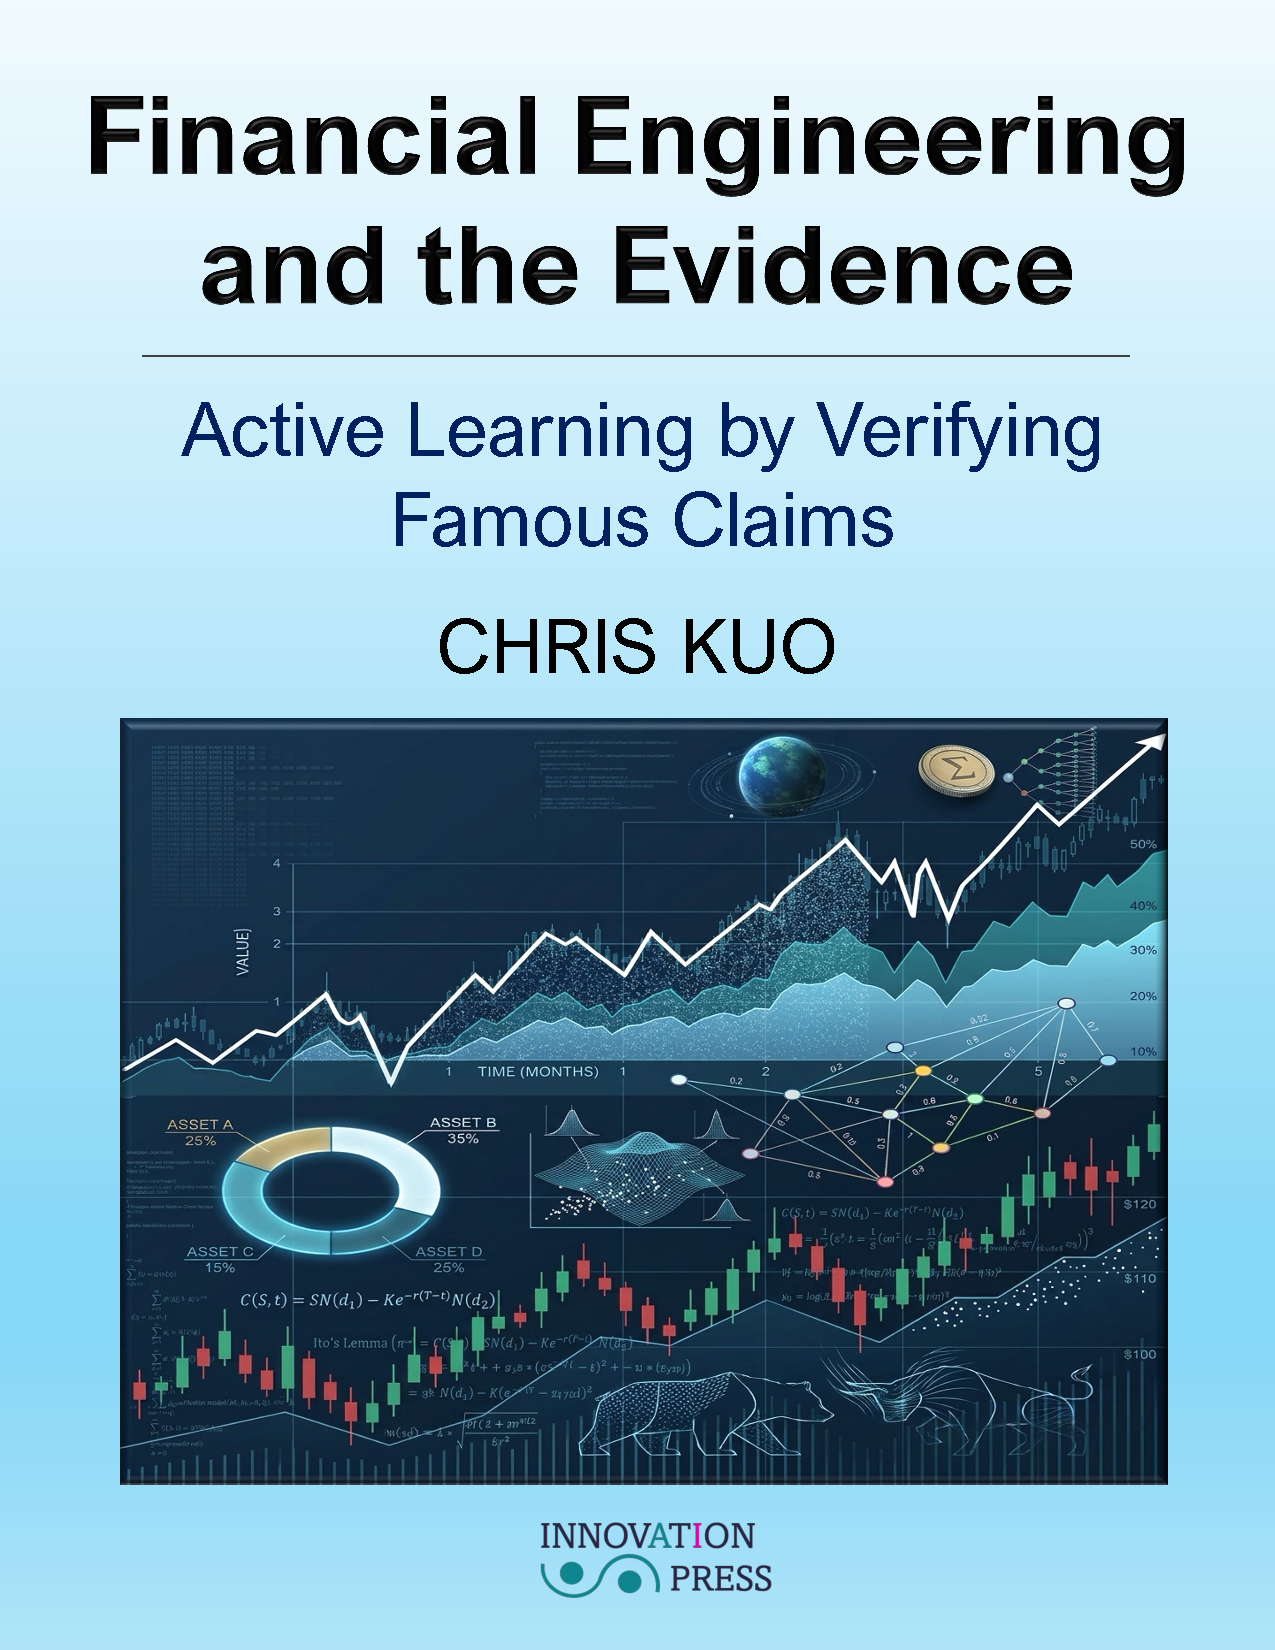
\includepdf{cover/The_frontcover_beautybook.pdf}


%------------------------ Publisher matter -------------------------%
\newpage
\vspace*{\fill}
\footnotesize
\noindent Copyright \textcopyright{} Chris Kuo, Ph.D. \\
\\
\noindent  All rights reserved. No part of this publication may be reproduced, stored in a retrieval system, or transmitted in any form or by any means, electronic, mechanical, photocopying, recording, scanning, or otherwise, except as permitted under Section 107 or 108 of the 1976 United States Copyright Act, without the prior written permission of the publisher, or in the case of brief quotations embodied in critical reviews and certain other noncommercial uses permitted by copyright law. 

\noindent  
While every effort has been made to ensure the reliability of the information presented in this publication, Innovation Press assumes no responsibility for errors or omissions. However, neither the author nor Innovation Press assumes any liability for damages resulting from the use of the information contained herein. \\
\\


 \noindent  ISBN 979-8-9825592-1-0
 \\
 \\
\noindent First edition:  January 2027 \\

\noindent This book was typeset using \LaTeX{} software. 
The  \TeX{}  template acknowledgement:  \\
 The \textit{Beautybook} \url{[https://ctan.org/pkg/beautybook?lang=en]} \\
Comprehensive TEX Archive Network (CTAN)\\
\\

 
\noindent The Innovation Press, \\
\noindent Ann Arbor, MI 
\begin{figure}[!htbp]
  
\includegraphics[width=0.12\textwidth]{innovation_press.png}% Replace example-image with the filename of your image
\end{figure}
 
\vspace*{\fill}
\normalsize
\pagenumbering{arabic}

% ---------------------------------------------------------------------------- %
%                           The Sidebar Theme Chosen                           %
% ---------------------------------------------------------------------------- %
\definecolor{bg}{HTML}{e0e0e0}
\definecolor{fg}{HTML}{2c4f54}
\colorlet{outermarginbgcolor}{bg}
\colorlet{outermarginfgcolor}{fg}
% set the contents of the outer margin on even and odd pages for scrheadings, plain and scth
\oddoutermargin{\sffamily \leftmark} % Odd
\evenoutermargin{\sffamily\@title} % Even

% ---------------------------------------------------------------------------- %
%                         The images used in the title                         %
% ---------------------------------------------------------------------------- %
\titleimage{
  chapteroddimage={odd1,odd2,odd3,odd4,odd5,odd6,odd7,odd8,odd9,odd10,odd11,odd12,odd13,odd14,odd15,mid1,mid2,mid3,mid4,mid5,mid6,mid7,mid8,mid9,mid10,mid11},
%
  partoddimage={odd1,odd2,odd3,odd4,odd5,odd6,odd7,odd8,odd9,odd10,odd11,odd12,odd13,odd14,odd15,mid1,mid2,mid3,mid4,mid5,mid6,mid7,mid8,mid9,mid10,mid11},
%
  chapterevenimage={songeven,even1,even2,even3,even4,mid1,mid2,mid3,mid4,mid5,mid6,mid7,mid8,mid9,mid10,mid11},
%
  partevenimage={songeven,even1,even2,even3,even4,mid1,mid2,mid3,mid4,mid5,mid6,mid7,mid8,mid9,mid10,mid11},
}
\chapimage{\Beautybook@chapterimagename}
\partimage{\Beautybook@partimagename}
\makeatother
\colorlet{framegolden}{fg} % The line color of the magic box
\colorlet{framegray}{bg!50} % The background color of the magic box
\frontmatter


% -------------------------About the author------------------------------%
{
\thispagestyle{empty}

\chapter*{About the Author}
\addcontentsline{toc}{chapter}{About the Author}

\textbf{Chris Kuo} is an economist, data scientist and educator with more than 25 years of experience in quantitative modeling and analytics. 
His work centers on applied artificial intelligence, machine learning and data-driven decision making. He has led data science initiatives in enterprise environments
and is the inventor of a U.S.\ patent for data-driven analytical solutions.

In addition to his industry work, Chris teaches at Columbia University and has previously taught at Boston University, the University of New Hampshire and Liberty University, in economics, management and machine learning. He believes that students learn a method best when they are asked to verify a statement with it, especially in the age of AI. That belief is the philosophy behind this book.
He has published research in economics and management journals and is the author of ten books on applied AI, machine learning and analytics.

He holds a Ph.D. in Economics from Stony Brook University and a B.S. in Nuclear Engineering from National Tsing Hua University in Taiwan. He lives in New York City with his wife.

\medskip
\noindent His published books include (by year):

\begin{enumerate}[label=\arabic*., leftmargin=*, itemsep=1pt, topsep=4pt]
  \item \textbf{2027}\quad\textit{Financial Engineering and the Evidence: Active Learning by Verifying Famous Claims}
  \item \textbf{2026}\quad\textit{Agentic AI for Anomaly Detection: Building Your Own Agentic AI Systems Step by Step}
  \item \textbf{2026}\quad\textit{Modern Causal Inference: Methods and Applications: An Essential Hands-on Guide with DoWhy, EconML, CausalML, Causal-learn in Python}
  \item \textbf{2025}\quad\textit{Introduction to Statistics with Python: The Essential Guide to Data Analysis}
  \item \textbf{2024}\quad\textit{The Handbook of Anomaly Detection (2nd Edition): Cutting-edge Methods and Hands-On Code Examples}
  \item \textbf{2024}\quad\textit{Modern Time Series Forecasting Techniques For Predictive Analytics and Anomaly Detection: From Classical Foundations to Cutting-Edge Applications}
  \item \textbf{2023}\quad\textit{The Handbook of NLP with Gensim: Leverage topic modeling to uncover hidden patterns, themes, and valuable insights within textual data}
  \item \textbf{2023}\quad\textit{The Handbook of Anomaly Detection (1st Edition): Build and modernize your anomaly detection models with examples}
  \item \textbf{2022}\quad\textit{Transfer Learning for Image Classification: With Python examples}
  \item \textbf{2022}\quad\textit{The eXplainable A.I.: With Python Examples}
  \item \textbf{2021}\quad\textit{Modern Time Series Anomaly Detection: With Python and R examples}
\end{enumerate}

% ---- Dedication -------------------------------------------------------
%\cleardoublepage
%\thispagestyle{empty}
%\vspace*{\fill}

%\begin{center}
%  \textit{This book is dedicated to Nathan and Eileen,}\\[4pt]
%  \textit{from Dad.}
%\end{center}

%\vspace{2cm}

%\noindent\rule{\textwidth}{0.8pt}
%\begin{center}
%  \begin{minipage}{0.85\textwidth}
%    \centering
%    ``Trust in the \textsc{Lord} with all your heart and lean not on your own
%    understanding; in all your ways submit to him, and he will make your
%    paths straight.''\\[6pt]
%    ---~Proverbs 3:5--6 (NIV)
%  \end{minipage}
%\end{center}
%\noindent\rule{\textwidth}{0.8pt}

%\vspace*{\fill}
}

%------------------------------TOC------------------------------------------%
\thispagestyle{empty}
\tableofcontents\let\cleardoublepage\clearpage

\mainmatter

% ----------------------------Preface and Introduction-----------------%

% Preface -- Financial Engineering and the Evidence
\chapter*{Preface}
\addcontentsline{toc}{chapter}{Preface}
\markboth{Preface}{Preface}

\emph{Financial Engineering and the Evidence: Active Learning by Verifying Famous Claims}

\section*{A natural way to learn}

For a long time I have been thinking about how people learn a technical subject, and how that learning could be more active and more inspiring.

Many textbooks follow a familiar pattern: a model is presented, its formulas are derived, a few examples are worked, and exercises follow at the end of the chapter. This is a time-tested way to pass on knowledge.

But it may not make a reader research-oriented, and it may not build the judgment a working quant needs most: knowing whether a result can be trusted. When I turn the question around and ask, ``Does this actually work? Let's find out,'' the classroom comes alive. Students make predictions, argue about what the data will show, run the numbers, and remember what they found, often because it was not what they expected.

I believe this is the natural way people learn, even in the age of AI. This book is built on that conviction. Its subtitle, \emph{Active Learning by Verifying Famous Claims}, describes the method. You will not be asked to accept the results of quantitative finance on authority. Instead, you will be invited to test those results for yourself while learning the techniques of financial engineering.

\section*{Why this approach, and why now}

Three developments make this the right moment for a book like this.

First, the evidence behind many famous claims is live and unresolved. For example, Hou, Xue and Zhang (2020) re-tested 452 published anomalies and found that about 65 percent fail a basic significance test once micro-caps are given little weight. Jensen, Kelly and Pedersen (2023), using a Bayesian method and data from 93 countries, concluded that most factors do replicate. Goyal, Welch and Zafirov (2024) found that many return predictors proposed since 2008 have lost their power. When leading researchers disagree, students need to be able to work through the disagreement themselves. This book is designed to bring students into such debates rather than only report their conclusions. In Chapter~\ref{ch:07}, for example, students replicate both sides of the anomaly debate and form their own view.

Second, the data to do so is now free. Kenneth French's data library, FRED, the Jensen--Kelly--Pedersen global factors and Chen and Zimmermann's Open Source Asset Pricing portfolios let any student rebuild published results without a paid database.

Third, new methods are entering finance faster than they are being tested. Machine learning and time series foundation models promise much, but the finance-specific evidence is mixed. Students need to learn where these tools help and where they do not, and the only way to know is to test them.

Courses that teach the replication debate usually do it through journal articles, while their textbooks present results rather than ask students to re-test them. This book is written to fill that gap.

\section*{Putting famous claims on trial}

Finance is full of famous claims. Past winners keep winning. The trend is your friend. Stock market returns are predictable. Optimized portfolios beat simple equal weighting. Machine learning predicts stock returns better than linear models.

Practitioners act on these claims, products are sold on them, and many are taught as if they were settled. They are also exactly the kind of question an active learner can answer with data.

In this book, every such claim is put on trial, and you are the one who tries it. Each claim chapter follows the same cycle:

\begin{enumerate}
  \item \textbf{Claim.} State what is asserted, in one testable sentence.
  \item \textbf{Understand.} Learn how the idea works and how the original evidence was produced.
  \item \textbf{Verify.} Rebuild the result in a Python lab on open data, then stress-test it out of sample, in other markets and after costs.
  \item \textbf{Judge.} Reach a dated verdict: survives, weakens, fails or provisional.
  \item \textbf{Apply.} Take away what investors and practitioners can use, and what remains open.
\end{enumerate}

This order is the heart of the active approach. Because the question comes first, every method is learned at the moment it is needed, to settle something you actually want to know. Newey--West errors, false-discovery rates and walk-forward evaluation stop being abstract tools and become the instruments that decide a case. Each lab also asks you to write down what you expect before you run a step. When the data disagree with your prediction, the surprise is visible, and it stays with you.

The verdicts are not foregone conclusions. Some claims largely survive, such as the predictability of volatility. Some survive only in weakened form, such as value and momentum. The goal is to follow the evidence wherever it leads, and on some questions, such as whether most published anomalies are false, serious researchers still disagree. There you will replicate both sides and write your own verdict.

Repeated across twenty-three claims, the cycle becomes a habit. That habit, more than any single verdict, is what I hope you take from this book: before believing a result, ask ``compared to what, out of sample, and after costs?''

\section*{How the book is organized}

The book has eight parts, twenty-three chapters and four appendices. Every chapter, from the first, puts a famous claim on trial, and the chapters are ordered so that each one introduces methods only a little harder than the ones before it. Read in order, the book is a single course that starts with averages and t-statistics and ends with machine learning and foundation models.

\begin{itemize}
  \item Part I tests claims about returns, luck and data, using means, Sharpe ratios, t-statistics and simulation.
  \item Part II tests claims about the cross-section of stock returns, using regression, factor models, portfolio sorts and trading costs.
  \item Part III tests claims about forecasting over time, in stocks, bonds and currencies, using out-of-sample evaluation.
  \item Part IV tests claims about portfolio construction and diversification.
  \item Part V tests claims about volatility and risk models.
  \item Part VI tests claims about options and credit.
  \item Part VII tests claims about machine learning, from tree ensembles to transformer-based asset-pricing models.
  \item Part VIII tests claims about time series foundation models and ends with a capstone in which you replicate a claim of your own choosing.
\end{itemize}

The parts are not marked by separate pages in the text. Table~\ref{tab:pref-parts} lists the chapters in each part.

\begin{table}[htbp]
\centering
\small
\caption{The eight parts of the book and their chapters.}
\label{tab:pref-parts}
\begin{tabularx}{0.95\linewidth}{@{}>{\raggedright\arraybackslash}p{0.07\linewidth}>{\raggedright\arraybackslash}p{0.28\linewidth}>{\raggedleft\arraybackslash}p{0.04\linewidth}>{\raggedright\arraybackslash}X@{}}
\toprule
Part & Theme & Ch. & Title \\
\midrule
I & Returns, luck and data & \ref{ch:01} & A Strong Track Record Proves Skill \\
 &  & \ref{ch:02} & Historical Data Show What a Strategy Would Have Earned \\
\addlinespace
II & Factor models and the cross-section & \ref{ch:03} & Size and Value Explain Returns That Beta Cannot \\
 &  & \ref{ch:04} & A Profitable Backtest Means a Profitable Strategy \\
 &  & \ref{ch:05} & Low-Risk Stocks Beat High-Risk Stocks \\
 &  & \ref{ch:06} & Past Winners Keep Winning \\
 &  & \ref{ch:07} & Most Published Anomalies Fail to Replicate \\
\addlinespace
III & Forecasting over time & \ref{ch:08} & Stock Market Returns Are Predictable \\
 &  & \ref{ch:09} & The Trend Is Your Friend \\
 &  & \ref{ch:10} & The Yield Curve Predicts Future Interest Rates \\
 &  & \ref{ch:11} & Currency Losses Cancel Out Higher Interest Rates \\
\addlinespace
IV & Portfolios and dependence & \ref{ch:12} & Optimized Portfolios Beat Simple Equal Weighting \\
 &  & \ref{ch:13} & Diversification Fails When You Need It Most \\
\addlinespace
V & Volatility and risk & \ref{ch:14} & Volatility Is Predictable \\
 &  & \ref{ch:15} & Value-at-Risk Models Measure Risk Reliably \\
\addlinespace
VI & Derivatives and credit & \ref{ch:16} & Selling Options Earns a Reliable Premium \\
 &  & \ref{ch:17} & Delta Hedging Removes Option Risk \\
 &  & \ref{ch:18} & Corporate Bond Spreads Mainly Reflect Expected Defaults \\
\addlinespace
VII & Machine learning & \ref{ch:19} & Machine Learning Predicts Stock Returns Better Than Linear Models \\
 &  & \ref{ch:20} & Artificial Intelligence Prices Stocks Better Than Factor Models \\
\addlinespace
VIII & Foundation models and the capstone & \ref{ch:21} & Foundation Models Forecast Better Than Classical Methods \\
 &  & \ref{ch:22} & Foundation Models Trained on Market Data Beat GARCH \\
 &  & \ref{ch:23} & Capstone: Replicating a Finance Claim \\
\bottomrule
\end{tabularx}
\end{table}


The claims were chosen so that testing them carries you through the standard curriculum of financial engineering. Each one rests on a core model: the CAPM, GARCH, Black--Scholes, the yield curve, the Merton model, mean--variance optimization. Every claim chapter opens with a self-contained Foundations section that teaches that model before the claim is tested. You meet the same material as in a conventional course, but you meet each model at the point where it makes a prediction the data can contradict.

This also means the book can stand on its own, or sit beside the classics. Hull, Cochrane, and Campbell, Lo and MacKinlay teach how the models are built. This book asks whether their predictions hold, and the table later in this preface shows, for each chapter, where those texts treat the topic in depth.

Every chapter has a Python lab. The book describes each lab by its question, data, setup and results, with tables and charts, so you can follow every argument without running any code. The code itself lives in a companion GitHub repository, where it can be kept working as data sources and libraries change. All labs run on free data, including the Kenneth French library, FRED and the open replication datasets now available, so no paid subscription is required.

\section*{Why these claims}

Each of the twenty-three claims, in Chapters~\ref{ch:01} to~\ref{ch:22}, was chosen to do two jobs at once: to settle a question that matters, and to teach a core model. The table shows how the claims map onto the standard curriculum. For each area of financial engineering, it lists the model or tool that the chapter's Foundations section teaches and the claim that puts it to work.

\begingroup
\small
\setlength{\LTpre}{6pt}\setlength{\LTpost}{6pt}
\begin{longtable}{@{}>{\raggedright\arraybackslash}p{0.198\linewidth}>{\raggedright\arraybackslash}p{0.288\linewidth}>{\raggedright\arraybackslash}p{0.297\linewidth}r@{}}
\toprule
Core area & Model or tool & Claim on trial & Ch. \\
\midrule
\endfirsthead
\toprule
Core area & Model or tool & Claim on trial & Ch. \\
\midrule
\endhead
\bottomrule
\endlastfoot
Statistics of returns & Returns, Sharpe ratio, t-statistics, luck by simulation & A strong track record proves skill & \ref{ch:01} \\
Financial data & Adjusted prices, survivorship, look-ahead and micro-cap biases & Historical data show what a strategy would have earned & \ref{ch:02} \\
Asset pricing and factors & OLS, the CAPM, factor models, robust standard errors & Size and value explain returns that beta cannot & \ref{ch:03} \\
Trading and implementation & Spreads, turnover, break-even costs, capacity & A profitable backtest means a profitable strategy & \ref{ch:04} \\
CAPM and leverage & Fama--MacBeth, GRS, beta estimation, leverage constraints & Low-risk stocks beat high-risk stocks & \ref{ch:05} \\
Market efficiency and behavior & Portfolio sorts, cross-sectional momentum, crash risk & Past winners keep winning & \ref{ch:06} \\
Econometrics of finance & False discovery rate, shrinkage, post-publication tests & Most published anomalies fail to replicate & \ref{ch:07} \\
Forecasting & Walk-forward evaluation, out-of-sample $R^2$, forecast comparison tests & Stock market returns are predictable & \ref{ch:08} \\
Technical analysis & Trading rules, time-series momentum, the Reality Check and SPA tests & The trend is your friend & \ref{ch:09} \\
Fixed income & Present value, yield curves, forward rates, duration, expectations hypothesis & The yield curve predicts future interest rates & \ref{ch:10} \\
International finance & Covered and uncovered interest parity, carry & Currency losses cancel out higher interest rates & \ref{ch:11} \\
Portfolio construction & Mean--variance, efficient frontier, covariance estimation & Optimized portfolios beat simple equal weighting & \ref{ch:12} \\
Diversification and dependence & Portfolio variance, correlation dynamics, tail dependence & Diversification fails when you need it most & \ref{ch:13} \\
Volatility modelling & ARCH/GARCH, realized and implied volatility & Volatility is predictable & \ref{ch:14} \\
Risk management & VaR, expected shortfall, backtesting, Basel & VaR models measure risk reliably & \ref{ch:15} \\
Options & Payoffs, put--call parity, implied volatility & Selling options earns a reliable premium & \ref{ch:16} \\
Derivative pricing and hedging & Black--Scholes, the Greeks, dynamic hedging & Delta hedging removes option risk & \ref{ch:17} \\
Credit & Default, recovery, spreads, the Merton model & Corporate bond spreads mainly reflect expected defaults & \ref{ch:18} \\
Machine learning & Regularization, trees, neural nets, cross-validation & Machine learning predicts stock returns better than linear models & \ref{ch:19} \\
Asset pricing with AI & Stochastic discount factor, IPCA, attention and transformers & Artificial intelligence prices stocks better than factor models & \ref{ch:20} \\
Forecasting with foundation models & ARIMA, exponential smoothing, zero-shot transformers & Foundation models forecast better than classical methods & \ref{ch:21} \\
Financial foundation models & Fine-tuning, range-based volatility, synthetic market data & Foundation models trained on market data beat GARCH & \ref{ch:22} \\
\end{longtable}
\endgroup

Each method is taught in the first chapter that needs it and is reused in the chapters that follow.

Every claim had to pass five tests before it earned a chapter.

\begin{enumerate}
  \item \textbf{Anchored in a core model.} Testing it requires you to learn a model that belongs in any financial engineering course.
  \item \textbf{Famous and consequential.} Practitioners act on it, products are sold on it, or it shaped the research literature.
  \item \textbf{Testable with free data.} Any student can run the lab with the French library, FRED, Shiller's data and similar public sources.
  \item \textbf{Still debated.} Recent papers disagree, so the verdict is not a foregone conclusion and your own test adds information.
  \item \textbf{A spread of verdicts.} Some claims largely survive (volatility is predictable), some survive only in weakened form (value, momentum, the option premium), and some largely fail (forward rates as forecasts, optimized portfolios beating an equal-weighted one). The method does not always say no.
\end{enumerate}

The claims do not cover everything. This is not a full treatment of stochastic calculus, exotic derivatives, term-structure models beyond the basics, corporate finance, or market microstructure at the level of the order book. 

\section*{Foundations sections by chapter}

Every chapter except the capstone opens its teaching with a Foundations section. It is not optional background: it sets out the concepts, formulas and terms that the rest of the chapter depends on, and it is part of what each chapter expects you to learn. Each Foundations section runs about two to three pages, with key terms in bold, the essential formulas and a worked example. The table below lists, for each chapter, the standard texts that treat its topic in depth. They are written so that a reader without a prior course in investments or financial engineering can follow every chapter, which lets the book stand on its own. You do not need the books in the Further reading column to follow this one. They are listed for readers who want a deeper treatment of a topic, now or later.

\begingroup
\small
\setlength{\LTpre}{6pt}\setlength{\LTpost}{6pt}
\begin{longtable}{@{}r>{\raggedright\arraybackslash}p{0.468\linewidth}>{\raggedright\arraybackslash}p{0.324\linewidth}@{}}
\toprule
Ch. & Foundations covers & Further reading \\
\midrule
\endfirsthead
\toprule
Ch. & Foundations covers & Further reading \\
\midrule
\endhead
\bottomrule
\endlastfoot
\ref{ch:01} & Simple, log and excess returns; the risk-free rate; expected return and volatility; the Sharpe ratio; standard errors and t-statistics & Bodie, Kane and Marcus (2024); Campbell, Lo and MacKinlay (1997) \\
\ref{ch:02} & Corporate actions and adjusted prices; index weighting; CRSP, Compustat, FRED and the French library; delisting; point-in-time data & Bodie, Kane and Marcus (2024); Bali, Engle and Murray (2016) \\
\ref{ch:03} & Moments of a distribution; OLS and its standard errors; the CAPM, beta and alpha; factor models & Wooldridge (2025); Bodie, Kane and Marcus (2024); Cochrane (2005) \\
\ref{ch:04} & Order books; bid--ask spreads; market and limit orders; short selling; long--short portfolios; turnover & Harris (2003); Bodie, Kane and Marcus (2024); Hull (2022) \\
\ref{ch:05} & The security market line; estimating beta; Fama--MacBeth and GRS tests; leverage constraints & Bodie, Kane and Marcus (2024); Ang (2014) \\
\ref{ch:06} & Measuring past returns; cross-sectional momentum; underreaction and overreaction & Bodie, Kane and Marcus (2024); Ilmanen (2011) \\
\ref{ch:07} & Market efficiency; what an anomaly is; replication and robustness; false discovery rates & Bodie, Kane and Marcus (2024); Bali, Engle and Murray (2016) \\
\ref{ch:08} & Loss functions; information sets; bias--variance; training, validation and test data; autoregressive models; walk-forward evaluation and leakage; out-of-sample $R^2$ and forecast comparison tests & Hyndman and Athanasopoulos (2021); L\'opez de Prado (2018) \\
\ref{ch:09} & Moving-average and breakout rules; time-series momentum; volatility targeting; the SPA test & Ilmanen (2011); Elliott and Timmermann (2016) \\
\ref{ch:10} & Present value; bond prices and yields; zero-coupon curves; forward rates; duration; the expectations hypothesis & Hull (2022); Tuckman and Serrat (2022) \\
\ref{ch:11} & Spot and forward exchange rates; covered and uncovered interest parity; carry & Hull (2022); Bodie, Kane and Marcus (2024) \\
\ref{ch:12} & Mean--variance optimization; the efficient frontier; estimating covariance matrices & Bodie, Kane and Marcus (2024); Luenberger (2014) \\
\ref{ch:13} & Portfolio variance and correlation; correlation over time; tail dependence & Bodie, Kane and Marcus (2024); Ang (2014) \\
\ref{ch:14} & Realized and implied volatility; ARCH and GARCH; the VIX & Hull (2022); Tsay (2010) \\
\ref{ch:15} & Value-at-risk and expected shortfall; historical, parametric and Monte Carlo methods; backtesting; Basel rules & Hull (2022, 2023) \\
\ref{ch:16} & Calls and puts; payoffs; put--call parity; implied volatility; the variance risk premium & Hull (2022) \\
\ref{ch:17} & The Black--Scholes model and its assumptions; delta, gamma and the Greeks; dynamic hedging & Hull (2022); Shreve (2004) \\
\ref{ch:18} & Default probability and recovery; credit spreads; ratings; the Merton model & Hull (2022) \\
\ref{ch:19} & Supervised learning; preparing inputs; penalized regression; trees, random forests and boosting; neural networks; tuning and interpreting models & James, Witten, Hastie and Tibshirani (2021); Hastie, Tibshirani and Friedman (2009); L\'opez de Prado (2018) \\
\ref{ch:20} & The stochastic discount factor; shrinkage and IPCA estimators; deep and adversarial SDFs; attention and transformers & Cochrane (2005); Kelly and Xiu (2023); Nagel (2021) \\
\ref{ch:21} & Classical forecasting models (ARIMA, exponential smoothing); transformers; zero-shot forecasting & Hyndman and Athanasopoulos (2021) \\
\ref{ch:22} & OHLCV data and range-based volatility; fine-tuning; synthetic market data; the Giacomini--White test & Hyndman and Athanasopoulos (2021); Goodfellow, Bengio and Courville (2016) \\
\end{longtable}
\endgroup

Chapter~\ref{ch:23}, the capstone, draws on all of these and has no Foundations section of its own. It also collects the research-design tools (hypotheses, power, pre-registration and robustness grids) that a replication needs.


Full references for these books are listed alphabetically by author under Further Reading at the end of the book (page~\pageref{furtherreading}).


\section*{Who this book is for}

This book is for anyone who builds, buys or studies quantitative strategies and needs to judge whether the evidence behind them holds up.

\begin{itemize}
  \item Students in financial engineering, quantitative finance and financial data science will use the whole book, labs included, as will quantitative analysts and researchers at asset managers, banks and fintech firms.
  \item PhD students can use it as a companion for the replication debate. Portfolio managers, allocators and serious individual investors can read the principles and verdicts and skim the labs.
\end{itemize}

You will need to possess basic Python, and to know introductory statistics, regression and the elements of investments. Everything else is taught along the way.

This is not a book of trading signals. If anything, its most consistent lesson is how rarely a promising backtest survives honest testing. What it offers instead is more durable: the ability to tell the difference.

\section*{An invitation}

Learning by verifying is slower at first than learning by reading. You will make predictions that turn out wrong, and you will spend time on results that do not hold. But you will understand each method because you needed it, and you will remember each verdict because you reached it yourself.

I wrote this book in the hope that it makes learning financial engineering more active and more enjoyable. Pick a claim, write down what you expect, and let the evidence decide.

\bigskip
\begin{flushright}
\emph{Chris Kuo}\\
\emph{January 2027}
\end{flushright}



% ---- Part I: Returns, luck and data
\part{Returns, Luck and Data}
% Chapter 1 -- Claim: A Strong Track Record Proves Skill (was Ch. 1)
% Requires: amsmath, booktabs, array, tabularx, graphicx, tcolorbox (breakable, skins), hyperref or url.
% Defines the callout box only if the preamble has not.
\providecolor{fenavy}{HTML}{1B2A6B}
\providecolor{feshade}{HTML}{F3F5FA}
\makeatletter
\@ifundefined{callout}{%
  \newtcolorbox{callout}{breakable, enhanced,
    colback=white, colframe=gray!70, boxrule=0.5pt, arc=1mm,
    borderline west={2.5pt}{0pt}{gray!70},
    left=8pt, right=8pt, top=4pt, bottom=4pt}%
}{}
\makeatother

\chapter{Claim: A Strong Track Record Proves Skill}
\label{ch:01}

Every year, a great many investment strategies are presented with impressive track records. Fund reports show steady equity curves, academic papers report significant t-statistics\index{t-statistic}, and online forums share backtests\index{backtest} that turned \$10,000 into a fortune. Some of these strategies are genuinely good. The challenge, for anyone who wants to build or choose one, is to recognize which.

That is harder than it looks, because financial data make it unusually easy to find patterns that are not there. Returns are noisy, the history is short, and everyone searches the same data. Under those conditions, a strategy with no skill at all can look brilliant for a while, and a genuinely good strategy can look ordinary for a decade. But real skill leaves evidence that luck cannot fake for long, and this chapter shows how to read it.

The claim on trial\index{claims-on-trial method} in this chapter is the one every strategy builder hopes is true: \textbf{a long enough track record can reveal real skill.} Testing it means learning how long ``long enough'' is, and what else a record must show. The chapter then introduces the method the rest of the book uses: state the claim, understand it, verify it, judge it, and apply what survives.

The chapter is built around two papers. Bailey, Borwein, L\'opez de Prado and Zhu (2014) show how easily a backtest can look brilliant when many strategies are tried and only the best one is reported. Harvey, Liu and Zhu (2016) ask how high the statistical bar must be once we account for all the strategies the profession has already tested. The lab in Section~\ref{sec:01-lab} replicates the logic of both papers in order to measure how good a track record luck alone can produce, and how much higher the bar must be before a record counts as evidence of skill.

By the end of the chapter you will be able to:

\begin{itemize}
  \item compute simple, log and excess returns\index{return!excess}, and convert monthly means and volatilities\index{volatility} to annual ones;
  \item calculate a Sharpe ratio\index{Sharpe ratio} and judge whether a mean return is statistically different from zero;
  \item distinguish profits that come from bearing risk, from luck and from skill, and measure skill as alpha\index{alpha};
  \item explain what market efficiency\index{efficient market hypothesis} implies for return predictability\index{return predictability}, and what it does not;
  \item calculate how many years of data are needed to tell a good strategy from luck;
  \item list the main ways a backtest can mislead;
  \item use the book's claims-on-trial method and verdict scale\index{verdict scale}.
\end{itemize}

In the lab you will generate 1,000 trading strategies that are random by construction, run them on nearly a century of real U.S. market data, and watch several of them look like the work of a genius. Because you know that every one of them is pure luck, you will see exactly what a real record must do to stand out from luck. That is the best preparation for judging and building the strategies you will meet in the rest of the book and in your career.

\section{Foundations: returns, risk and the Sharpe ratio}
\label{sec:01-foundations}

\subsection{Returns}

The \textbf{simple return}\index{return!simple|textbf} on an asset over a period is the gain in price plus any income, divided by the starting price:
\begin{equation}
  R_t = \frac{P_t + D_t - P_{t-1}}{P_{t-1}}
  \label{eq:01-return}
\end{equation}
where $P$ is the price and $D$ is any dividend or coupon paid during the period. A return that includes income is a \textbf{total return}\index{return!total|textbf}; one that does not is a price return. The \textbf{log return}\index{return!log|textbf}, $r = \ln(1 + R)$, is convenient because log returns add over time: the log return over a year is the sum of the twelve monthly log returns. Simple returns, by contrast, compound: \$1 grows to $(1 + R_1)(1 + R_2)\cdots(1 + R_n)$.

\subsection{The risk-free rate and excess returns}
\label{sec:01-rf}

The return on a short-term government bill, such as a one-month U.S. Treasury bill, is treated as the \textbf{risk-free rate}\index{risk-free rate|textbf}, $R_f$: it is known in advance and carries essentially no default risk. 
The \textbf{excess return}\index{return!excess|textbf} of an asset is its return minus the risk-free rate. If $R_{i,t}$ denotes the return on asset $i$ in period $t$ and $R_{f,t}$ denotes the risk-free rate for the same period, the excess return is
\begin{equation}
R^{e}_{i,t} = R_{i,t} - R_{f,t}.
\label{eq:excess-return}
\end{equation}
Excess returns measure what an investor earns for bearing risk, and most of finance is about them. Following Cochrane (2005), this book writes an excess return as $R^{e}$ and reserves a lowercase $r$ for log returns.

The average excess return of the stock market over bills is the \textbf{equity premium}\index{equity premium|textbf}. Writing $R_{m,t}$ for the return on the market portfolio, the equity premium is
\begin{equation}
E\left[R^{e}_{m,t}\right] = E\left[R_{m,t} - R_{f,t}\right],
\label{eq:equity-premium}
\end{equation}
and its sample estimate over $T$ periods is
\begin{equation}
\bar{R}^{e}_{m} = \frac{1}{T}\sum_{t=1}^{T} R^{e}_{m,t} = \frac{1}{T}\sum_{t=1}^{T}\left(R_{m,t} - R_{f,t}\right).
\label{eq:equity-premium-sample}
\end{equation}




\subsection{Expected return and volatility}
\label{sec:01-expret}

An asset's \textbf{expected return}\index{return!expected|textbf}, $E[R]$, is the average return an investor anticipates; it is never observed directly and must be estimated from history or from a model. Risk is usually measured by the \textbf{standard deviation}\index{standard deviation|textbf} of returns, called \textbf{volatility}\index{volatility|textbf}. Monthly figures are converted to annual ones by multiplying the mean by 12 and the standard deviation by $\sqrt{12}$, which assumes returns in different months are uncorrelated. For U.S. stocks over the last century, the annual equity premium has averaged roughly 6 to 8 percent with volatility near 20 percent, so a single year's return tells us very little about the expected return.

\subsection{Why one year tells us so little}

The problem is the size of the noise relative to the signal. Take an expected excess return of 7\%, the middle of that range, and a volatility of 20\%. The volatility is almost three times the expected return, so the randomness in any single year swamps the reward we are trying to measure. Figure~\ref{fig:01-oneyear} shows the range of outcomes this implies.

\begin{enumerate}
  \item \textbf{Ordinary years are far from the average.} About two years in three fall within one standard deviation of the expected return, between $7 - 20 = -13$\% and $7 + 20 = 27$\%. A gain of 27\% and a loss of 13\% are both ordinary years, even though the expected return is the same 7\% in each.
  \item \textbf{Large swings are normal.} About 95\% of years fall within two standard deviations, $7 \pm 1.96 \times 20$, or roughly $-32$\% to 46\%. A year like 2008, when U.S. stocks fell by more than a third, lies just beyond this range. Such a year is rare, but it is not out of character for a market this volatile.
  \item \textbf{Losing years are common.} Even though stocks are expected to beat bills by 7\% a year, 
  the excess return is negative in about 36\% of years, or roughly one year in three. A single bad year is therefore no evidence that the equity premium has disappeared, and a single good year is no evidence that it is large.
  \item \textbf{Averaging helps, but slowly.} Averaging over $T$ years shrinks the noise in the estimate to $20/\sqrt{T}$ percent. After 10 years the standard error is still about 6.3\%, so the average could plausibly lie anywhere from about $-5$\% to 19\%. Even after 100 years it is 2\%, giving a 95\% range of about 3\% to 11\%. This is why, after a century of data, researchers can say only that the equity premium is ``roughly 6 to 8 percent'' rather than give a precise number.
\end{enumerate}

The same arithmetic, applied to the Sharpe ratio rather than the average return, is what makes strategies so hard to evaluate in Section~\ref{sec:01-signal-noise}.

\providecolor{fenavy}{HTML}{1B2A6B}

\begin{figure}[!htbp]
  \centering
  \begin{tikzpicture}[
    % One-year excess return ~ Normal(mean 7%, s.d. 20%)
    declare function={
      mu = 7; sd = 20;
      pdf(\x) = exp(-0.5*((\x-mu)/sd)^2)/(sd*sqrt(2*pi));
    }]
  \begin{axis}[
    width=0.82\linewidth, height=0.42\linewidth,
    axis lines=left,
    axis line style={-stealth, thin},
    xmin=-63, xmax=77, ymin=0, ymax=0.023,
    xtick={-53,-33,-13,7,27,47,67},
    ytick=\empty,
    xlabel={One-year excess return (\%)},
    ylabel={Likelihood},
    samples=200, domain=-63:77,
    clip=false,
  ]
    \addplot[name path=dens, draw=none] {pdf(x)};
    \path[name path=base] (axis cs:-63,0) -- (axis cs:77,0);

    % Plus or minus one standard deviation: -13% to 27%
    \addplot[fill=fenavy!22, draw=none]
      fill between[of=dens and base, soft clip={domain=-13:27}];
    % Below zero
    \addplot[fill=gray!60, fill opacity=0.6, draw=none]
      fill between[of=dens and base, soft clip={domain=-63:0}];

    % Edges of the one-sigma band
    \draw[fenavy] (axis cs:-13,0) -- (axis cs:-13,{pdf(-13)});
    \draw[fenavy] (axis cs:27,0)  -- (axis cs:27,{pdf(27)});

    % Density curve on top
    \addplot[fenavy, thick] {pdf(x)};

    % Expected return
    \draw[thick, dashed] (axis cs:7,0) -- (axis cs:7,0.0215)
      node[above] {expected 7\%};

    % Labels
    \node[anchor=west] at (axis cs:-64,0.0122) {below zero: 36\%};
    \node[fenavy, anchor=west] at (axis cs:25,0.0165)
      {$\pm 1\sigma$: $-13\%$ to $27\%$};
  \end{axis}
  \end{tikzpicture}
  \caption{One year's excess return on the stock market, assuming an expected excess return of 7\% and volatility of 20\%. The blue band covers the middle two-thirds of years, from $-13$\% to 27\%; the gray area is the 36\% of years with a negative excess return.}
  \label{fig:01-oneyear}
\end{figure}


%\begin{figure}[htbp]
%\centering
%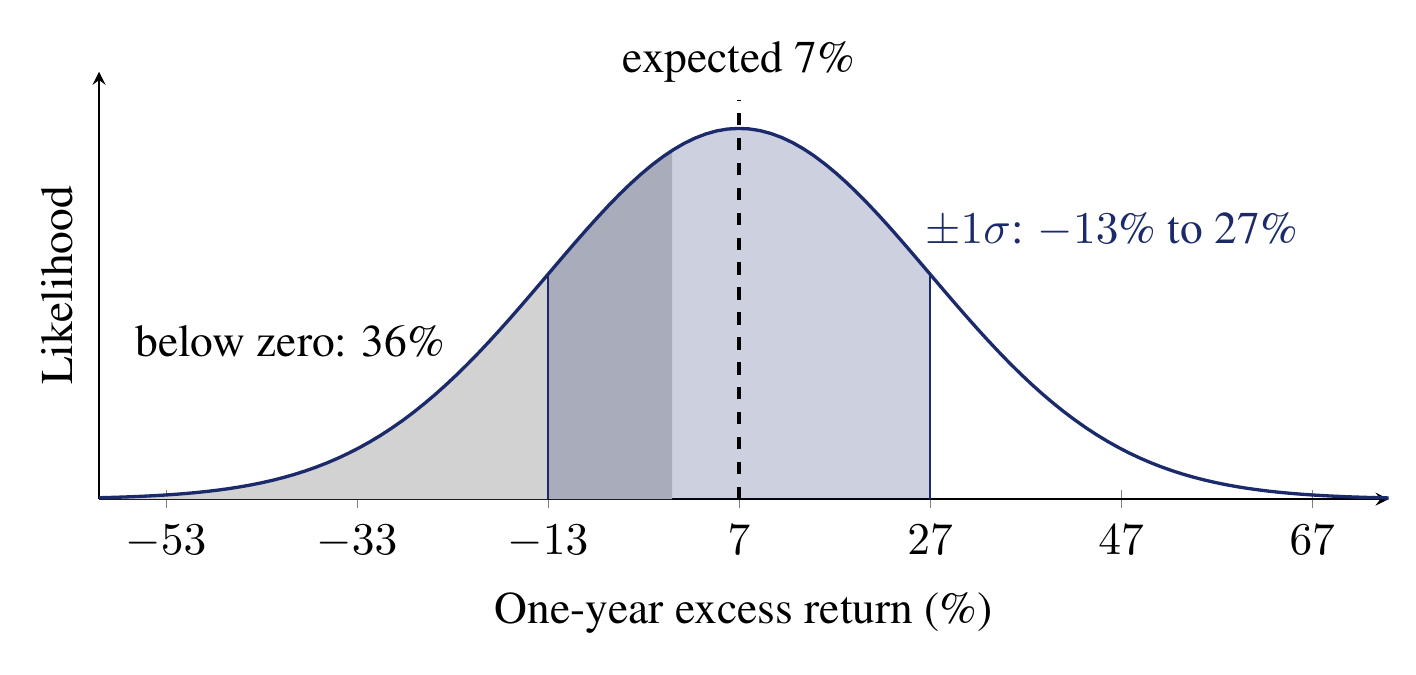
\includegraphics[width=0.85\linewidth]{images/fig01-1-one-year-return.png}
%\caption{One year's excess return on the stock market, assuming an expected excess return of 7\% and volatility of 20\%. The blue band covers the middle two-thirds of years, from $-13$\% to 27\%; the gray area is the 36\% of years with a negative excess return.}
%\label{fig:01-oneyear}
%\end{figure}


\subsection{The Sharpe ratio}
\label{sec:01-sharpe}

Sharpe (1966) proposed judging an investment by its excess return per unit of risk:
\begin{equation}
  \mathrm{SR} = \frac{E[R] - R_f}{\sigma} = \frac{E[R^{e}]}{\sigma}
  \label{eq:01-sr}
\end{equation}

The stock market's long-run Sharpe ratio is around 0.3 to 0.4 a year. Because leverage\index{leverage} scales excess return and volatility equally, the Sharpe ratio does not change when a portfolio is levered up or down, which makes it the natural measure for comparing strategies (Figure~\ref{fig:01-sharpe-slope}).

%\begin{figure}[htbp]
%\centering
%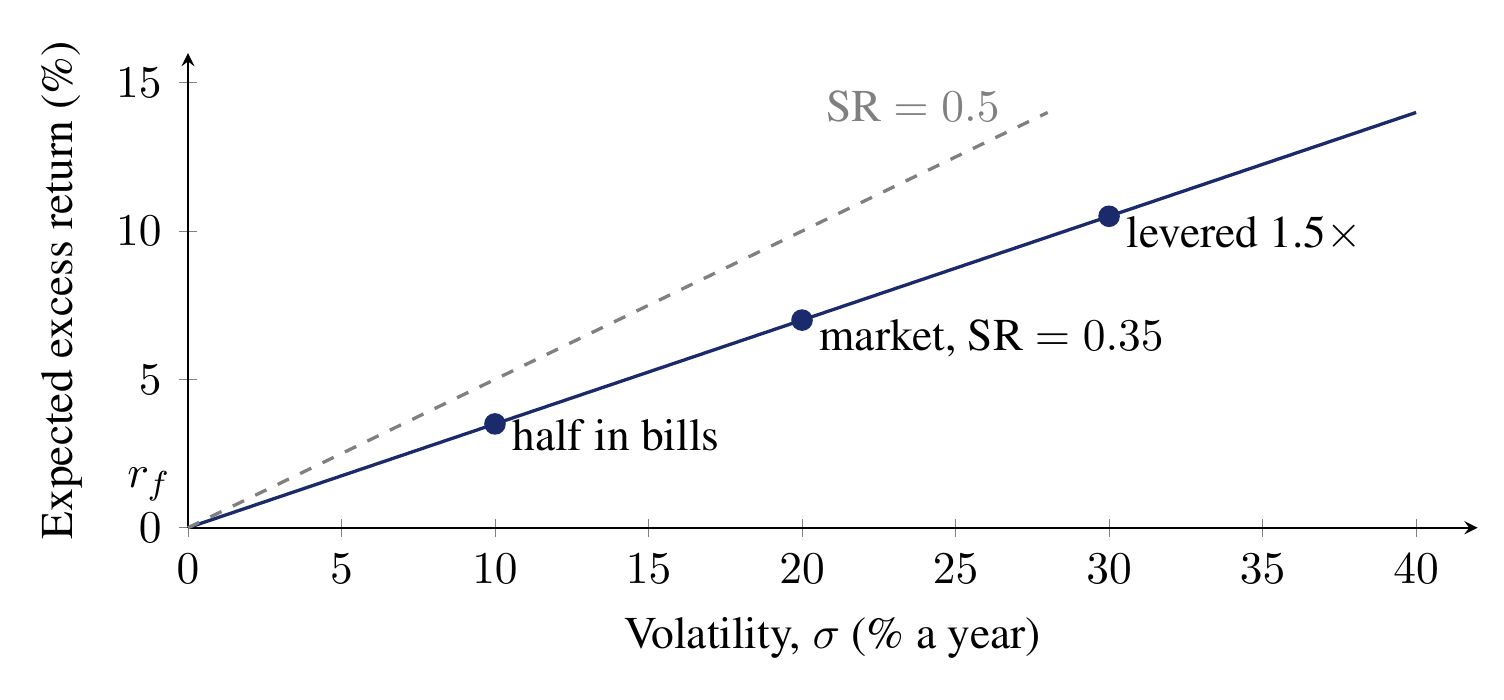
\includegraphics[width=0.85\linewidth]{images/fig01-2-sharpe-slope.png}
%\caption{The Sharpe ratio is the slope of a line from the risk-free rate. Leverage moves a portfolio along its line, raising or lowering both excess return and volatility, but does not change the slope. A better strategy lies on a steeper line.}
%\label{fig:01-sharpe-slope}
%\end{figure}

\providecolor{fenavy}{HTML}{1B2A6B}

\begin{figure}[!htbp]
  \centering
  \begin{tikzpicture}
  \begin{axis}[
    width=0.8\linewidth, height=0.42\linewidth,
    axis lines=left,
    axis line style={-stealth, thin},
    xmin=0, xmax=41, ymin=0, ymax=16,
    xtick={0,5,...,40},
    ytick={0,5,10,15},
    xlabel={Volatility, $\sigma$ (\% a year)},
    ylabel={Expected excess return (\%)},
    clip=false,
  ]
    % A higher Sharpe ratio, for comparison
    \addplot[gray, thick, dashed, domain=0:28, samples=2] {0.5*x};
    \node[gray, anchor=south] at (axis cs:23,14) {SR $= 0.5$};

    % Capital allocation line through the market (Sharpe ratio 0.35)
    \addplot[fenavy, thick, domain=0:40, samples=2] {0.35*x};

    % Portfolios on the line
    \fill[fenavy] (axis cs:10,3.5)  circle (2.6pt);
    \fill[fenavy] (axis cs:20,7)    circle (2.6pt);
    \fill[fenavy] (axis cs:30,10.5) circle (2.6pt);
    \node[anchor=north west, inner sep=2pt] at (axis cs:10.3,3.5) {half in bills};
    \node[anchor=north west, inner sep=2pt] at (axis cs:20.3,7)   {market, SR $= 0.35$};
    \node[anchor=north west, inner sep=2pt] at (axis cs:30.3,10.5) {levered $1.5\times$};

    % Risk-free asset at the origin
    \node[anchor=east] at (axis cs:-0.6,1.6) {$R_f$};
  \end{axis}
  \end{tikzpicture}
  \caption{The Sharpe ratio is the slope of a line from the risk-free rate. Leverage moves a portfolio along its line, raising or lowering both excess return and volatility, but does not change the slope. A better strategy lies on a steeper line.}
  \label{fig:01-sharpe-slope}
\end{figure}


\subsection{Risk, luck and skill}

Investors who make money in the stock market can do so for three different reasons. The distinction runs through the whole book.


\begin{itemize}
  \item \textbf{Bearing risk.} Stocks are riskier than Treasury bills, so over
  time they have paid more. This extra return is the equity premium defined
  above. An investor who simply buys and holds an index fund earns it without
  any special ability. Profit from bearing risk is a reward for risk, not
  evidence of skill.

  Here are three examples. (i) A retiree who has held an S\&P~500 index fund since
  1990 has earned far more than a savings account would have paid, without
  ever picking a stock. (ii) A manager who borrows to hold the index at
  1.5 times exposure beats the index in most years, but only because he
  carries 1.5 times its risk; in a crash he loses 1.5 times as much.
  (iii) A trader who sells out-of-the-money\index{option!moneyness} put options\index{option!put} collects a small,
  steady premium month after month and looks like a genius, until a market
  crash wipes out years of gains. In each case the extra return is payment
  for risk that anyone could have taken.

  \item \textbf{Luck.} Returns are noisy, so some investors do well by
  chance, sometimes for years at a time. We also hear more about the winners
  than the losers, which makes luck look more common than it is.

  Here are three examples. (i) Ten thousand people each flip a coin every year to
  decide whether to hold stocks or cash. After ten years, about ten of them
  will have called the market right every single year, and some will write
  books about their method. (ii) A newsletter sends 1{,}000 readers a
  ``buy'' call on a stock and another 1{,}000 a ``sell'' call. Whichever way
  the stock moves, half the readers now hold a correct prediction, and the
  trick can be repeated on that half. (iii) An investor puts her savings into
  one small biotech company just before it receives surprise drug approval.
  Her gain was real, but it rests on a single draw, so it says almost nothing
  about her ability.


  \item \textbf{Skill.} Skill is the ability to earn more than the risk taken
  explains. It produces a return that a simple, cheap alternative carrying the
  same risk would not have delivered. Skill usually comes from better
  information, better analysis or better execution.

  Here are three examples, one of each kind. 
  With \textbf{(i) better
  information}, an analyst counts cars in retailers' parking lots from
  satellite images and forecasts sales before the companies report them.
  With \textbf{(ii) better analysis}, a fund beats a portfolio with the same
  market, size and value exposures, after fees, over twenty years and across
  many independent bets. 
  With \textbf{(iii) better execution}, a trading firm
  buys and sells the same stocks as everyone else but pays less in trading
  costs\index{transaction costs} and price impact\index{market impact}. It keeps a few basis points\index{basis point} per trade that others
  give away.

  
  Researchers and practitioners have documented several cases that are widely
  regarded as genuine skill, and they fall into the same three groups.
  
  \begin{enumerate}
    \item \textbf{Better information.} The parking-lot example is not hypothetical.
  Katona, Painter, Patatoukas and Zeng (2025) found that investors who bought
  satellite data on retailers' parking lots were able to trade profitably
  ahead of earnings announcements, especially when the news was bad. Cohen,
  Frazzini and Malloy (2008) found that mutual fund managers earned higher
  returns on stocks of companies whose senior officers had attended the same
  university as the manager, which suggests that information can travel
  through personal networks. Cohen, Malloy and Pomorski (2012) separated
  corporate insiders who trade on a regular schedule from those who break
  their routine. The routine trades carried little information, while the
  unusual trades predicted future returns.

    \item \textbf{Better analysis.} Kosowski, Timmermann, Wermers and White (2006)
  used a bootstrap\index{bootstrap} to ask whether the best mutual fund records could be
  produced by luck alone. They concluded that a minority of managers appear
  to pick stocks well enough to cover their costs, and that their records are
  difficult to explain by chance. Berk and van Binsbergen (2015) measured
  skill as the dollars a fund adds rather than as a percentage return. By
  that measure, the typical manager adds value, and differences in skill
  persist for many years. Kacperczyk, Sialm and Zheng (2005) found that funds
  concentrating on a few industries tend to outperform after adjusting for
  risk, consistent with managers who specialize in areas they understand well.

    \item \textbf{Better execution.} Frazzini, Israel and Moskowitz (2018) studied the
  actual trades of a large asset manager and found that its trading costs
  were much lower than the estimates used in many academic studies. Careful
  execution can therefore turn a strategy that looks unprofitable on paper
  into one that works in practice. Baron, Brogaard, Hagstr\"om{}er and
  Kirilenko (2019) found large and persistent differences in performance
  among high-frequency trading firms, and much of the difference was
  explained by how fast each firm could trade.
  
  \end{enumerate}

  Within the industry, the most frequently cited example is the Medallion
  Fund of Renaissance Technologies, whose exceptionally strong record over
  several decades is difficult to attribute to luck or to ordinary risk
  (Zuckerman, 2019). It is worth keeping these examples in proportion,
  however. Fama and French (2010) found that, after fees, very few mutual
  funds show evidence of skill, even though some do before fees. Genuine
  skill appears to exist, but it seems to be rare, and much of its value is
  often captured by the managers rather than passed on to investors.
  
  
\end{itemize}

\noindent\textbf{Exercise: which one is it?} Suppose an investor
consistently chooses the right stock at the right time. Before calling this
skill, ask two questions. First, \emph{does the risk explain it?} If the
investor's picks are mostly high-risk stocks bought during a rising market,
a cheap fund holding equally risky stocks might have done just as well, and
the profit is a reward for risk. Second, \emph{does luck explain it?} If the
record is short, or the investor is one of many whose picks we never hear
about, a run of good calls is what chance alone would produce. Only when the
answer to both questions is no does skill become the likely explanation. The
rest of this section shows how finance measures it.

\textbf{Finance measures skill with alpha}. Regress a strategy's excess return on the market's excess return:
\begin{equation}
  R^{e}_{s} = \alpha + \beta\, R^{e}_{m} + \varepsilon \nonumber
\end{equation}
where $R^{e}_{s} = R_s - R_f$ is the strategy's excess return, $R^{e}_{m} = R_m - R_f$ is the market's excess return, as in Equation~\eqref{eq:excess-return}, and $\varepsilon$ is the part of the return the regression does not explain. The coefficient $\beta$ (\textbf{beta}\index{beta|textbf}) measures how much market risk the strategy carries, so $\beta\, R^{e}_{m}$ is the return that market exposure alone would have delivered. The intercept $\alpha$ is what is left over, that is, the average return beyond what the strategy's market risk explains. For example, suppose a strategy has a beta of 0.6 and earns an average excess return of 6\% a year while the market earns 8\%. Market risk explains $0.6 \times 8 = 4.8$\%, so the strategy's alpha is $6 - 4.8 = 1.2$\% a year. Chapter~\ref{ch:03} develops this regression and its extensions to other sources of risk.

A positive alpha is necessary for skill but not sufficient, because luck also produces positive alphas. Telling the two apart is the central problem of this chapter.

\subsection{Estimating a mean, and how uncertain the estimate is}
\label{sec:01-se}

Given $T$ independent observations of a return with standard deviation $\sigma$, the sample mean $\bar{R}$ has a \textbf{standard error}\index{standard error|textbf} of
\begin{equation}
  \mathrm{SE}(\bar{R}) = \frac{\sigma}{\sqrt{T}}.
  \label{eq:01-se}
\end{equation}
The standard error measures how far the sample mean is likely to fall from the true mean, and it shrinks only with the square root of the number of observations, so quadrupling the data merely halves it. The \textbf{t-statistic}\index{t-statistic|textbf} of a mean is the estimate divided by its standard error; under the hypothesis that the true mean is zero, it has approximately a standard normal distribution\index{distribution!normal}, so values beyond about $\pm 1.96$ occur by chance only 5\% of the time. Applied to the Sharpe ratio, the same arithmetic gives a useful rule: the t-statistic of a strategy's mean return is approximately its annual Sharpe ratio times the square root of the number of years. A Sharpe ratio of 0.5
needs about 15 years of data before the t-statistic of its mean return reaches 1.96 (Figure~\ref{fig:01-years}).

%\begin{figure}[htbp]
%\centering
%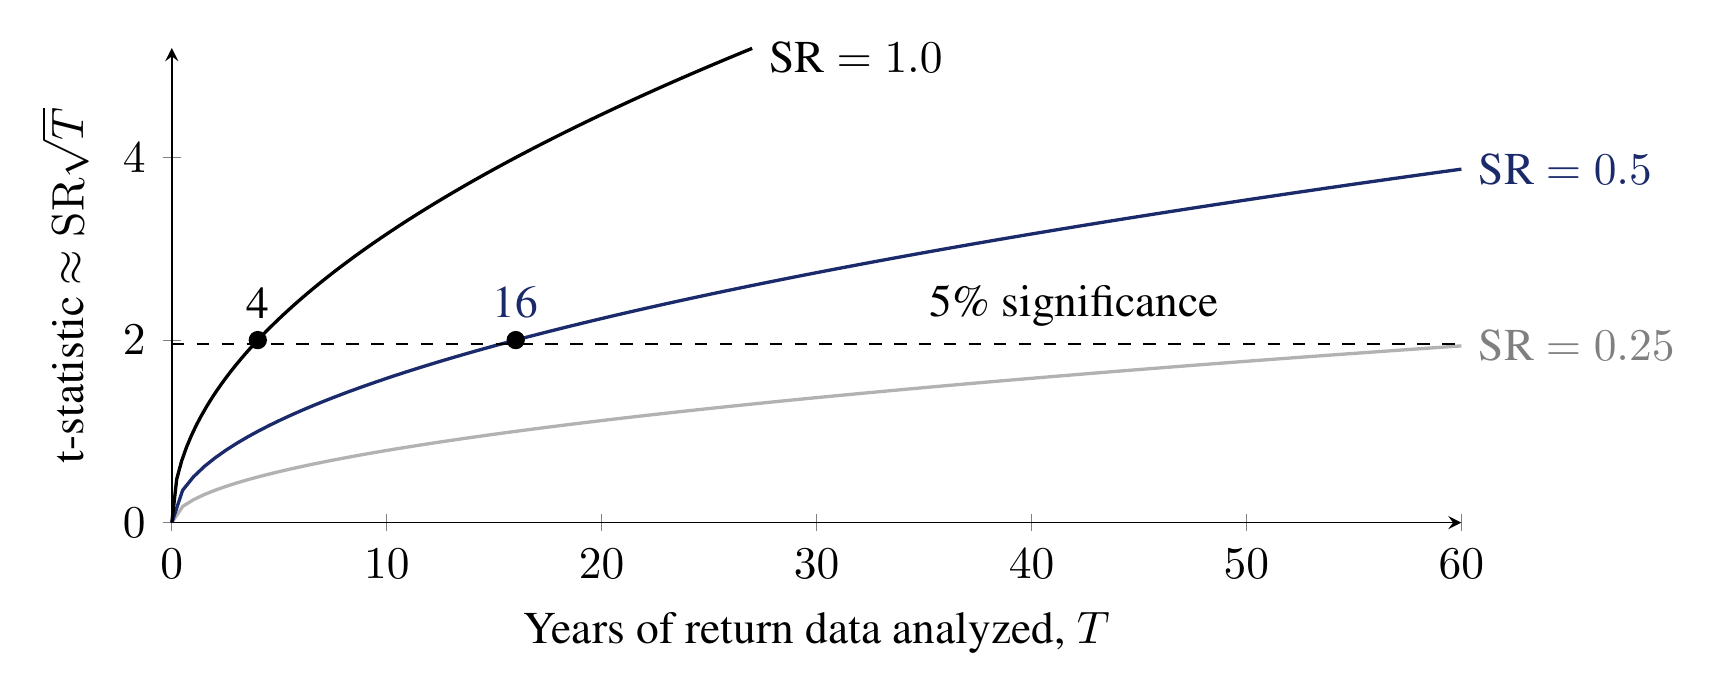
\includegraphics[width=0.85\linewidth]{images/fig01-3-years-needed.png}
%\caption{How many years of return data are needed before a strategy's track record becomes statistically significant. The years count the length of the history being analyzed, not how long the strategy must trade or hold its positions. With a true Sharpe ratio of 0.5, about 15 years of data are needed to reach $t = 1.96$; with 0.25, about 61.}
%\label{fig:01-years}
%\end{figure}


\providecolor{fenavy}{HTML}{1B2A6B}

\begin{figure}[!htbp]
  \centering
  \begin{tikzpicture}
  \begin{axis}[
    width=0.78\linewidth, height=0.4\linewidth,
    axis lines=left,
    axis line style={-stealth, thin},
    xmin=0, xmax=61, ymin=0, ymax=5.4,
    xtick={0,10,...,60},
    ytick={0,2,4},
    xlabel={Years of return data analyzed, $T$},
    ylabel={t-statistic $\approx \mathrm{SR}\sqrt{T}$},
    samples=200,
    clip=false,
  ]
    % 5% significance
    \addplot[thick, dashed, domain=0:60, samples=2] {2};
    \node[anchor=south] at (axis cs:40,2.05) {5\% significance};

    % t = SR * sqrt(T) for three Sharpe ratios
    \addplot[thick, black, domain=0:27] {1.0*sqrt(x)};
    \addplot[thick, fenavy, domain=0:60] {0.5*sqrt(x)};
    \addplot[thick, gray!55, domain=0:60] {0.25*sqrt(x)};

    \node[anchor=west] at (axis cs:28,{sqrt(27)}) {SR $= 1.0$};
    \node[fenavy, anchor=west] at (axis cs:60.5,{0.5*sqrt(60)}) {SR $= 0.5$};
    \node[gray, anchor=west] at (axis cs:60.5,{0.25*sqrt(60)}) {SR $= 0.25$};

    % Years needed to reach t = 2
    \fill (axis cs:4,2)  circle (2.4pt);
    \fill (axis cs:16,2) circle (2.4pt);
    \node[anchor=south] at (axis cs:4,2.08) {4};
    \node[fenavy, anchor=south] at (axis cs:16,2.08) {16};
  \end{axis}
  \end{tikzpicture}
  \caption{How many years of return data are needed before a strategy's track record becomes statistically significant. The years count the length of the history being analyzed, not how long the strategy must trade or hold its positions. With a true Sharpe ratio of 0.5, about 15 years of data are needed to reach $t = 1.96$. With a Sharpe ratio of 0.25, about 61 years are needed.}
  \label{fig:01-years}
\end{figure}



\textbf{Worked example.} A strategy earns an average excess return of 0.5\% a month with a monthly standard deviation of 4\% over 10 years. Its annual mean is 6\%, its annual volatility is 4\% $\times \sqrt{12} \approx 13.9$\%, and its Sharpe ratio is $6/13.9 \approx 0.43$. The t-statistic is $0.5 / (4/\sqrt{120}) \approx 1.37$. This is not significant at the 5\% level, even though the strategy may be genuinely good.

%\textbf{Further reading.} Bodie, Kane and Marcus, \emph{Investments}, chapters on risk, return and the historical record; Campbell, Lo and MacKinlay, \emph{The Econometrics of Financial Markets}, chapter 1 on returns; Cochrane, \emph{Asset Pricing}, for the theory of why expected returns differ.


\section{Efficient markets and the random walk}
\label{sec:01-efficient-markets}

The starting point for any claim about beating the market is the efficient market hypothesis. In Eugene Fama's (1970) formulation, a market is efficient if prices fully reflect available information. The intuition comes from competition. If a predictable profit existed, traders would act on it, and their trading would push prices until the profit disappeared.

Fama distinguished three versions by the information set\index{forecasting!information set}:

\begin{center}
\small
\begin{tabularx}{0.9\linewidth}{@{}>{\raggedright\arraybackslash}p{0.180\linewidth}>{\raggedright\arraybackslash}p{0.234\linewidth}>{\raggedright\arraybackslash}X@{}}
\toprule
Version & Prices reflect & Implication if true \\
\midrule
Weak form & Past prices and trading volume & Technical trading rules cannot earn abnormal returns \\
Semi-strong form & All public information & Analysis of public news and accounting data cannot earn abnormal returns \\
Strong form & All information, including private & Even insiders cannot earn abnormal returns \\
\bottomrule
\end{tabularx}
\end{center}

Few economists believe the strong form\index{efficient market hypothesis!strong form}, and insider-trading laws exist because it fails. The weak and semi-strong forms are where the empirical debate happens, and where most claims in this book live.

\textbf{What efficiency does not imply.} Efficiency is often misread, so three clarifications matter:

\begin{enumerate}
  \item \textbf{It does not mean returns are unpredictable in every sense.} Expected returns can vary over time or across stocks as compensation for risk. A predictable return that is fair payment for risk is consistent with efficiency, but a predictable return that is a free lunch is not. Separating the two is known as the joint-hypothesis problem\index{joint-hypothesis problem}, because every test of efficiency is also a test of a model of what returns \emph{should} be.
  \item \textbf{It does not mean prices are always right.} It means mispricings are hard to identify and profit from after costs. Grossman and Stiglitz (1980) showed that a perfectly efficient market is impossible, because if prices reflected everything, no one would pay to gather information. Markets must be inefficient enough to reward the people who make them efficient.
  \item \textbf{It does not mean volatility is unpredictable.} As Chapter~\ref{ch:14} shows, risk is far more predictable than return.
\end{enumerate}

\textbf{The random walk\index{random walk} as a benchmark.} If prices respond only to new, unpredictable information, price changes should look approximately like a random walk, in which tomorrow's change is unrelated to today's. Samuelson (1965) showed that properly anticipated prices fluctuate randomly. Lo and MacKinlay (1988) later rejected a strict random walk for weekly U.S. returns, so the model is not literally true. Even so, it remains the right benchmark, and any strategy must beat what a random walk, or a simple buy-and-hold position, would deliver.

For this book, the practical lesson is a prior belief that we bring to every claim. Before seeing any evidence, we should treat a claim that a simple rule beats the market as unlikely. Such a claim is not impossible, since the following chapters find some rules that survive, but it is unlikely enough to demand strong evidence.

\section{Signal and noise}
\label{sec:01-signal-noise}

The deeper reason claims are hard to verify is statistical. In finance, the signal is small and the noise is large. The differences between good and bad strategies are a few percent a year in expected return, while their returns move by fifteen or twenty percent a year at random.

\textbf{The Sharpe ratio, again.}\index{Sharpe ratio|textbf} The yardstick for a strategy is the Sharpe ratio of Equation~\eqref{eq:01-sr}. In this section we write $\mu = E[R^{e}]$ for the strategy's expected excess return, so that $\mathrm{SR} = \mu/\sigma$, with all quantities annualized. The rest of the book uses $\mu$ in the same way. Against the stock market's long-run Sharpe ratio of 0.3 to 0.4 (Section~\ref{sec:01-foundations}), a strategy with a true Sharpe ratio of 0.5 after costs would be a valuable discovery, and 1.0 would be exceptional.

\textbf{How precisely can we measure it?} With $T$ years of independent returns, the t-statistic for testing whether the true Sharpe ratio is zero is approximately
\begin{equation}
  t \approx \mathrm{SR}\,\sqrt{T}
  \label{eq:01-t}
\end{equation}
Equation~\eqref{eq:01-t} follows from the definition of the Sharpe ratio in Equation~\eqref{eq:01-sr} in four steps.

\begin{enumerate}
  \item \textbf{Estimate the mean.} Take $T$ years of annual excess returns. Their sample average, $\bar{R}^{e}$, is our estimate of the expected excess return $\mu$.
  \item \textbf{Find its standard error.} If the yearly returns are independent with volatility $\sigma$, the standard error of an average of $T$ of them is
  \begin{equation}
    \mathrm{SE}(\bar{R}^{e}) = \frac{\sigma}{\sqrt{T}} \nonumber
  \end{equation}
  \item \textbf{Form the t-statistic.} To test whether the true mean is zero, divide the estimate by its standard error:
  \begin{equation}
    t = \frac{\bar{R}^{e}}{\sigma/\sqrt{T}} = \frac{\bar{R}^{e}}{\sigma}\,\sqrt{T} \nonumber
  \end{equation}
  \item \textbf{Recognize the Sharpe ratio.} The ratio $\bar{R}^{e}/\sigma$ is the measured Sharpe ratio. Replacing $\bar{R}^{e}$ with the true mean $\mu$ gives the t-statistic we should expect on average:
  \begin{equation}
    t \approx \frac{\mu}{\sigma}\,\sqrt{T} = \mathrm{SR}\,\sqrt{T} \nonumber
  \end{equation}
  The result is approximate for two reasons: the measured mean differs from the true one, and in practice $\sigma$ must be estimated as well.
\end{enumerate}

The answer is the same with monthly or daily data. Sampling $k$ times a year gives $kT$ observations, each with mean $\mu/k$ and volatility $\sigma/\sqrt{k}$, so
\begin{equation}
  t = \frac{\mu/k}{(\sigma/\sqrt{k})/\sqrt{kT}} = \frac{\mu}{\sigma}\,\sqrt{T} \nonumber
\end{equation}
and the sampling frequency $k$ cancels.

By the same reasoning, the standard error of an estimated annual Sharpe ratio is roughly $1/\sqrt{T}$. Lo (2002) gives the refinements for non-normal and autocorrelated returns, but the rough version is enough to see the problem. Setting $t = 1.96$, the usual 5\% significance threshold, in Equation~\eqref{eq:01-t} and solving for $T$ gives the number of years needed before a strategy's record can be distinguished from luck. Dividing both sides by SR gives $\sqrt{T} \approx 1.96/\mathrm{SR}$, and squaring gives
\begin{equation}
  T \approx \left(\frac{1.96}{\mathrm{SR}}\right)^2
  \label{eq:01-T}
\end{equation}

\begin{center}
\small
\begin{tabular}{@{}ll@{}}
\toprule
True Sharpe ratio & Years of data needed for the mean return to reach $t = 1.96$ \\
\midrule
0.25 & 61 \\
0.50 & 15 \\
0.75 & 7 \\
1.00 & 4 \\
1.50 & 2 \\
\bottomrule
\end{tabular}
\end{center}

A strategy as good as the stock market itself needs more than two decades of data before its record is statistically convincing. Most fund track records, and most backtests shown to investors, are far shorter.

\textbf{Does the return frequency matter?} For the years-needed table above, it does not. Daily data give 252 observations a year instead of 12, but each daily return carries proportionally less information about the mean, so the years needed are the same. Table~\ref{tab:01-frequency} shows this for one strategy observed over the same 16 years at three frequencies. The strategy has an expected excess return of 10\% a year and a volatility of 20\%, so its Sharpe ratio is 0.5. The t-statistic is always the Sharpe ratio \emph{per period} times the square root of the \emph{number of periods}. Sampling more often multiplies the number of observations, but shrinks the Sharpe ratio of each one by the square root of that factor, and the two effects cancel.

\begin{table}[htbp]
\centering
\small
\caption{The same 16-year record measured annually, monthly and daily. The expected excess return is 10\% a year and the volatility is 20\% a year, so the annual Sharpe ratio is 0.5. The daily figures assume 252 trading days a year.}
\label{tab:01-frequency}
\begin{tabular}{@{}lrrrrrr@{}}
\toprule
Frequency & Observations & Mean per & Volatility per & Sharpe ratio & $\sqrt{N}$ & $t$ \\
 & $N$ & period (\%) & period (\%) & per period & & \\
\midrule
Annual  & 16    & 10.000 & 20.00 & 0.500  & 4.00  & 2.00 \\
Monthly & 192   & 0.833  & 5.77  & 0.144  & 13.86 & 2.00 \\
Daily   & 4{,}032 & 0.040 & 1.26  & 0.0315 & 63.50 & 2.00 \\
\bottomrule
\end{tabular}
\end{table}

Going from annual to monthly data gives 12 times as many observations, but each has a mean 12 times smaller and a volatility $\sqrt{12}$ times smaller, so its Sharpe ratio is $\sqrt{12}$ times smaller. Since $\sqrt{N}$ grows by exactly $\sqrt{12}$, the t-statistic does not change. The same happens with 252 in place of 12 for daily data. This is why Equation~\eqref{eq:01-t} can be stated in years. $T$ counts observations only when the Sharpe ratio is measured over the same period, and for an annual Sharpe ratio that period is a year. Merton (1980) made the general point that the precision of an estimated expected return depends on the length of the history, not on the sampling frequency. With log returns the reason is especially plain. The average annual log return over $T$ years depends only on the first and last prices,
\begin{equation}
  \bar{r} = \frac{\ln P_T - \ln P_0}{T}, \nonumber
\end{equation}
because every price in between is added once and subtracted once. Dividing a century into days rather than months adds no information about the mean, and its standard error stays at about $20/\sqrt{100} = 2$\%, as in Section~\ref{sec:01-foundations}. The same holds for every claim about \emph{average} returns, such as the equity premium, value, momentum\index{momentum} and published anomalies\index{anomaly}, which is why Chapters~\ref{ch:03} to~\ref{ch:07} can test them on monthly data without losing anything.

Claims about \emph{risk} are different. Each additional observation adds information about how much returns vary, so the precision of an estimated volatility grows with the number of returns $N$, not just the number of years:
\begin{equation}
  \mathrm{SE}(\hat{\sigma}) \approx \frac{\sigma}{\sqrt{2N}} \nonumber
\end{equation}
With 20\% volatility and a century of data, the standard error is about 0.41 percentage points with monthly returns ($N = 1{,}200$) and about 0.09 with daily returns ($N \approx 25{,}200$), more than four times smaller. This is why the chapters on volatility (Chapter~\ref{ch:14}), value at risk\index{Value at Risk (VaR)} (Chapter~\ref{ch:15}), delta hedging\index{delta hedging} (Chapter~\ref{ch:17}) and trading costs (Chapter~\ref{ch:04}) use daily or even intraday data.

The rule ``the mean needs a long history, risk needs frequent data'' is a good guide, but it has limits.
\begin{itemize}
  \item \textbf{Very high frequency adds noise.} At intraday frequencies, the bounce between bid and ask prices and stale quotes distort measured returns, so for volatility, more frequent data help only up to a point.
  \item \textbf{Daily betas can be biased.} Stocks that trade infrequently react to market news with a delay, which makes their daily betas too low. Monthly data, or a correction that adds lagged market returns to the regression (Dimson, 1979), reduces the bias. This matters for the low-risk anomaly\index{low-risk anomaly} in Chapter~\ref{ch:05}.
  \item \textbf{Annualizing is not automatic.} The rules in Section~\ref{sec:01-foundations} for converting monthly figures to annual ones assume that returns are uncorrelated over time. When they are autocorrelated, as for many hedge funds and illiquid assets, a monthly Sharpe ratio multiplied by $\sqrt{12}$ can be badly off (Lo, 2002).
  \item \textbf{The cancellation is exact only for log returns.} For simple returns, the precision of the mean still depends mainly on the length of the history, but only approximately.
\end{itemize}

The practical lesson is to match the data to the claim. To measure an expected return more precisely, you need a longer history, not more frequent data. To measure risk, more frequent data do help.

\textbf{What a ten-year record can tell you.} The ``10 years'' here is not how long the strategy holds its positions, since the strategy may trade daily or monthly. It is the length of the track record you look at when you judge the strategy. A thought experiment shows how noisy that judgment is.

\begin{enumerate}
  \item \textbf{The strategy is genuinely good.} Suppose its true Sharpe ratio is 0.5. Nobody can see this number directly. We see only the Sharpe ratio measured from its realized returns\index{return!realized}.
  \item \textbf{The measurement is noisy.} With a 10-year record, the standard error of the measured Sharpe ratio is about $1/\sqrt{10} \approx 0.32$.
  \item \textbf{The record could show almost anything.} A 95\% range for the measured Sharpe ratio is $0.5 \pm 1.96 \times 0.32$, or about $-0.1$ to 1.1. Imagine watching the same strategy over many different decades. In one decade it looks like a star, with a Sharpe ratio near 1.0. In another it looks like a failure, with a Sharpe ratio near zero. The strategy is the same, and only the decade differs.
  \item \textbf{Luck can look like skill.} A strategy with no skill has a true Sharpe ratio of zero, yet its measured Sharpe ratio exceeds 0.5 whenever the noise is more than $0.5/0.32 \approx 1.6$ standard errors. That happens in roughly 6\% of decades, by luck alone.
\end{enumerate}

Figure~\ref{fig:01-ten-year} draws the two cases side by side. The curves overlap heavily. A measured Sharpe ratio of 0.4, for example, is quite consistent with both a genuinely good strategy and a useless one. A ten-year record cannot reliably tell them apart.

\providecolor{fenavy}{HTML}{1B2A6B}
\providecolor{fegray}{HTML}{4D4D4D}

\begin{figure}[!htbp]
  \centering
  \begin{tikzpicture}[
    % Estimated Sharpe ratio from a 10-year record: s.e. = 1/sqrt(10)
    declare function={
      se = 1/sqrt(10);
      npdf(\x,\m) = exp(-0.5*((\x-\m)/se)^2)/(se*sqrt(2*pi));
    }]
  \begin{axis}[
    scale only axis, width=0.7\linewidth, height=0.3\linewidth,
    axis lines=left,
    axis line style={-stealth, thin},
    xmin=-1.25, xmax=1.8, ymin=0, ymax=1.6,
    xtick={-1,-0.5,0,0.5,1,1.5},
    xticklabel style={/pgf/number format/fixed},
    ytick=\empty,
    ylabel={Likelihood},
    xlabel={Sharpe ratio measured from a 10-year record},
    xlabel style={yshift=-28pt},
    samples=200,
    clip=false,
  ]
    % No skill: true SR = 0
    \addplot[name path=null, fegray, thick, domain=-1.25:1.6] {npdf(x,0)};
    \path[name path=base] (axis cs:-1.25,0) -- (axis cs:1.8,0);
    % No-skill records above 0.5
    \addplot[fill=gray!40, draw=none]
      fill between[of=null and base, soft clip={domain=0.5:1.6}];

    % Good strategy: true SR = 0.5
    \addplot[fenavy, thick, domain=-0.75:1.8] {npdf(x,0.5)};

    % Centers
    \draw[fegray, dashed] (axis cs:0,0) -- (axis cs:0,{npdf(0,0)});
    \draw[fenavy, dashed] (axis cs:0.5,0) -- (axis cs:0.5,{npdf(0.5,0.5)});
    \node[fegray, anchor=south east, align=center] at (axis cs:0.05,1.3)
      {no skill\\(true SR $= 0$)};
    \node[fenavy, anchor=south west, align=center] at (axis cs:0.45,1.3)
      {good strategy\\(true SR $= 0.5$)};

    % Share of no-skill records above 0.5
    \node[fegray, anchor=south west, align=left] at (axis cs:1.12,0.62)
      {no-skill records\\above 0.5: about 6\%};
    \draw[-stealth, gray] (axis cs:1.2,0.6) -- (axis cs:0.78,0.17);

    % 95% range of the good strategy's measured Sharpe ratio
    \draw[fenavy, thick, |<->|] (axis cs:-0.12,-0.33) -- (axis cs:1.12,-0.33);
    \node[fenavy, anchor=north] at (axis cs:0.5,-0.36)
      {95\% of decades: $-0.1$ to $1.1$};
  \end{axis}
  \end{tikzpicture}
  \caption{What a 10-year record can show. The gray curve is the range of Sharpe ratios a strategy with no skill produces over different decades, and the blue curve is the same for a strategy with a true Sharpe ratio of 0.5. The shaded tail is the 6\% of decades in which the useless strategy beats 0.5 by luck.}
  \label{fig:01-ten-year}
\end{figure}


%\begin{figure}[htbp]
%\centering
%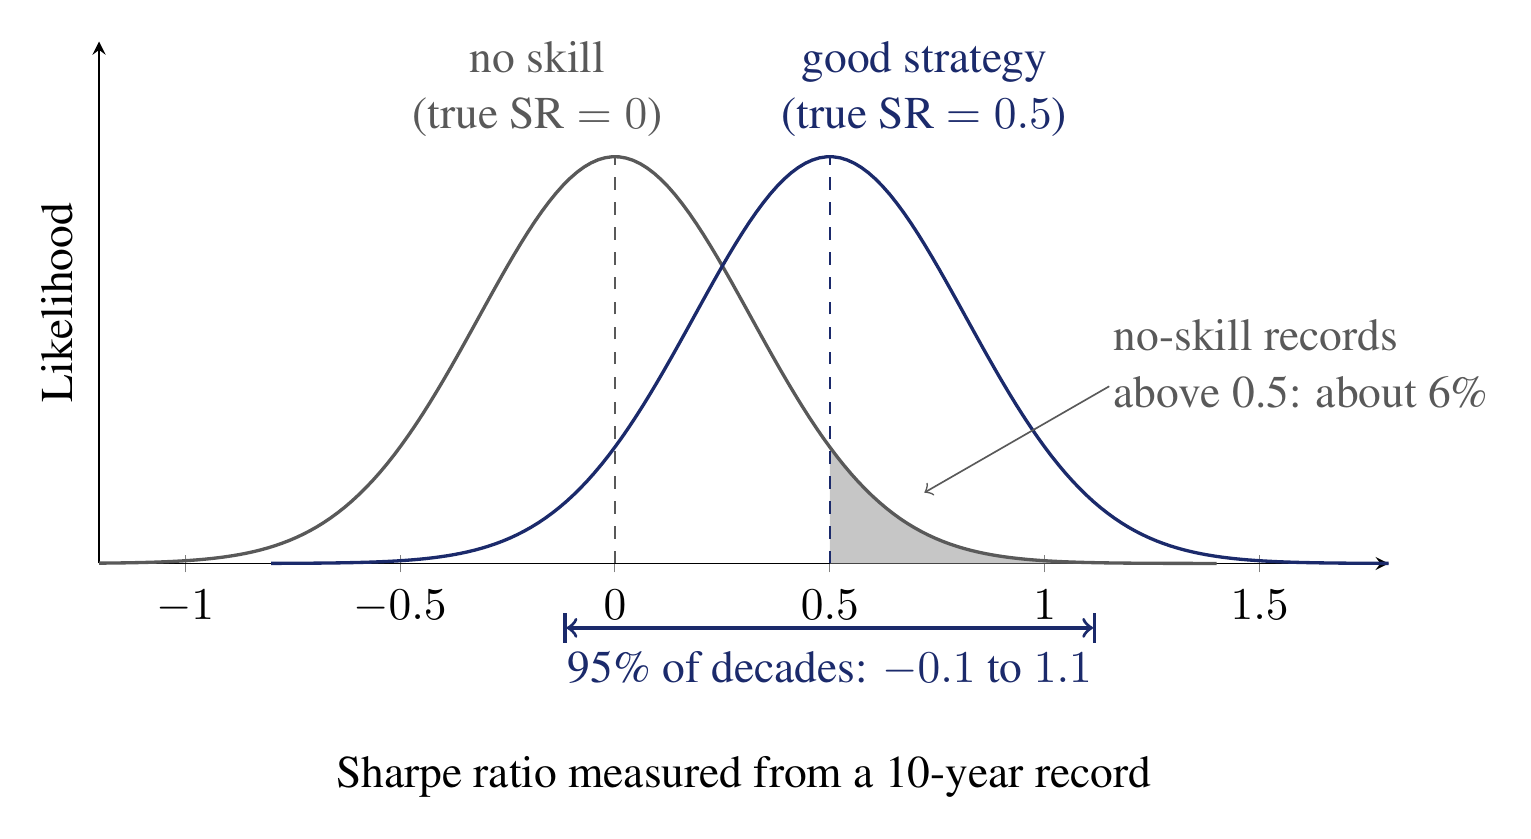
\includegraphics[width=0.85\linewidth]{images/fig01-4-ten-year-record.png}
%\caption{What a 10-year record can show. The gray curve is the range of Sharpe ratios a strategy with no skill produces over different decades; the blue curve is the same for a strategy with a true Sharpe ratio of 0.5. The shaded tail is the 6\% of decades in which the useless strategy beats 0.5 by luck.}
%\label{fig:01-ten-year}
%\end{figure}

\textbf{Why prediction is harder than it looks.} The same arithmetic applies to forecasting. A model that explains just 1\% of the variation in monthly returns would be worth a great deal to an investor (Campbell and Thompson 2008 make this point). But an $R^2$\index{regression!R-squared@$R^2$} of 1\% is almost impossible to distinguish from zero in a few decades of data, and almost trivially easy to produce by accident when many models are tried. Small true effects, large noise and short samples together make finance a field where false discoveries are easy and true ones are hard to confirm.

\section{Cautions: why backtests can mislead}
\label{sec:01-backtests}

A backtest applies a strategy's rules to historical data to show how it would have performed. It is the most common evidence offered for a strategy and the easiest to get wrong. Seven problems account for most misleading backtests; later chapters treat each in depth.

\begin{enumerate}
  \item \textbf{Selection across many trials.} If you test 100 rules and report the best, its record overstates what it will deliver. This is the subject of the lab, and Chapters~\ref{ch:07} and~\ref{ch:23} return to it.
  \item \textbf{Overfitting parameters.}\index{overfitting|textbf} Tuning a rule's settings, such as choosing a 47-day average instead of 50 or a threshold of 1.3 instead of 1.5, fits the noise in the sample. Each added parameter is another hidden trial.
  \item \textbf{Look-ahead bias.}\index{look-ahead bias|textbf} A backtest may use information that was not available at the time, such as revised economic data, or accounting figures before their release date (Chapter~\ref{ch:02}).
  \item \textbf{Survivorship bias.}\index{survivorship bias|textbf} A backtest may test only companies or funds that still exist, which leaves out the ones that failed (Chapter~\ref{ch:02}).
  \item \textbf{Ignoring costs.} Spreads, commissions, market impact, borrowing fees\index{borrowing fee} and taxes\index{taxes} can erase a paper profit, especially for high-turnover\index{turnover} strategies (Chapter~\ref{ch:04}).
  \item \textbf{Short or unrepresentative samples.} A decade of data may contain only one market regime. As Section~\ref{sec:01-signal-noise} showed, a short sample cannot separate skill from luck.
  \item \textbf{A story told after the fact.} Once a pattern is found, a plausible explanation is easy to write. The story makes the result feel robust, but it was written to fit the data, not tested against it.
\end{enumerate}

These problems compound. A backtest can be honest in every visible detail, using correct prices, real costs and no look-ahead, and still mislead because it is the best of many attempts that are never shown.

\begin{callout}
\textbf{What Failed: butter in Bangladesh.} To show how easy data mining\index{data mining} is, David Leinweber searched a United Nations database for series that tracked the S\&P 500. Butter production in Bangladesh fit well. Adding U.S. cheese production and the sheep population of Bangladesh and the United States raised the fit further, until the $R^2$ looked like a breakthrough. The relationship, of course, predicted nothing afterward. The example was a joke with a serious point: if you search enough series, you are guaranteed to find a near-perfect fit. Leinweber later wrote it up as ``Stupid Data Miner Tricks'' (2007).
\end{callout}

\section{The claims-on-trial method and the verdict scale}
\label{sec:01-method}

Every claim chapter and every lab opens with a line labelled \textbf{Claim on trial}\index{claims-on-trial method|textbf}. The label is a reminder of who does the work. You are not told whether the claim is true; you test it yourself. The book's subtitle, \emph{Active Learning by Verifying Famous Claims}, describes the bargain. Each trial needs a method (a regression, a backtest, a volatility model, a hedge), and you learn that method in order to reach a verdict, then use it again in later trials until it is second nature.

The rest of this book applies one method to every claim. It is simple enough to remember and strict enough to protect against the problems in Section~\ref{sec:01-backtests}.

\begin{enumerate}
  \item \textbf{Claim} --- State what is asserted in one testable sentence. ``Momentum works'' is vague; ``stocks with the highest 12-month returns, skipping the last month, outperform the lowest by a positive average return after costs'' can be tested.
  \item \textbf{Understand} --- Learn how the idea works and how the original evidence was produced, including the data, the sample period, the method and the number of alternatives the authors tried.
  \item \textbf{Verify} --- Rebuild the result yourself, then stress-test it out of sample\index{in-sample versus out-of-sample}, in other markets, after costs and after publication.
  \item \textbf{Judge} --- Reach a verdict on the scale below, and date it with the sample period you tested.
  \item \textbf{Apply} --- State what an investor or practitioner can actually use, and what remains open.
\end{enumerate}

\textbf{The verdict scale}\index{verdict scale|textbf}

\begin{center}
\small
\begin{tabularx}{0.9\linewidth}{@{}>{\raggedright\arraybackslash}p{0.162\linewidth}>{\raggedright\arraybackslash}X@{}}
\toprule
Verdict & Meaning \\
\midrule
Survives & The result replicates, holds out of sample and in other markets, and remains economically meaningful after costs. \\
Weakens & The result is real but smaller, less reliable, or narrower than claimed, for example only in small stocks or before publication. \\
Fails & The result does not replicate, or disappears out of sample or after costs. \\
Provisional & The evidence is too new or too mixed for a firm verdict. \\
\bottomrule
\end{tabularx}
\end{center}

Two habits make the method work. First, \textbf{decide the test before seeing the result}. Write down the claim, the data and the pass criteria in advance, so that the test cannot be bent to fit the outcome. Second, \textbf{always ask ``compared to what?''} Every claim is judged against a simple benchmark, such as the market, the historical average\index{historical-mean benchmark} or a naive rule, and never against zero.

This chapter's lab applies the method to a claim at the root of the whole field: whether a track record can reveal real skill.

\section{Lab~\thechapter: Brilliant by chance}
\label{sec:01-lab}

\begin{callout}
\textbf{Lab~\ref{ch:01} at a glance.} The claim on trial is that a long enough track record can reveal real skill. The lab uses monthly U.S. market excess returns and Treasury bill rates since 1926 from the Kenneth R. French Data Library\index{Kenneth French data library}, which the code downloads automatically. You will work in Python with pandas, NumPy and matplotlib, plus the book's fintest module. The lab takes about one hour, including the guided notebook, although the code itself runs in seconds. The code is in the repository folder \texttt{ch01-brilliant-by-chance/}.
\end{callout}

\subsection*{Design}

The design of this lab rests on two influential papers. Bailey, Borwein, L\'opez de Prado and Zhu (2014) show that the best of many backtests can look impressive by chance alone. Harvey, Liu and Zhu (2016) argue that the usual $t > 2$ hurdle is far too low when many strategies are tried. Following their logic, the lab answers the claim by first measuring what luck alone can do. It builds strategies that we know for certain have no skill at all. Whatever these strategies achieve sets the bar that a real strategy's record must clear. Every month, each of the 1,000 strategies is either invested in the stock market or holding Treasury bills. It switches between the two at random, with an average holding period between 3 and 24 months, so the strategies look like real market-timing rules. They use no information at all, and each month's position is fixed before that month's return is known.

The sample is split in two. The first half, roughly 1926 to 1975, plays the role of the \textbf{backtest}\index{backtest|textbf}. This is the period in which a researcher would test the strategies and choose the best. The second half, roughly 1976 to today, is the period \textbf{after selection}. It shows what an investor who adopted the chosen strategy would have experienced.

\textbf{Measuring skill.} A strategy that is in the market part of the time will earn part of the market's return with no skill at all. Skill is therefore measured as \textbf{alpha against buy-and-hold} (Section~\ref{sec:01-foundations}), which is the intercept in a regression of the strategy's excess return on the market's excess return. For every strategy in this lab, the true alpha is zero. The significance of each alpha is measured by its t-statistic, computed with Newey--West\index{standard error!Newey--West (HAC)} standard errors, which Chapter~\ref{ch:03} explains. We write this statistic as $t_\alpha$. Throughout the lab, every t-statistic is $t_\alpha$, and the tests are one-sided\index{hypothesis testing!one-sided and two-sided}, because only a positive alpha would suggest skill. A strategy with $t_\alpha > 1.96$ therefore has an alpha that is significantly positive at the usual threshold.

\subsection*{Three parts}

\begin{enumerate}
  \item \textbf{Signal and noise.}\index{signal and noise|textbf} Measure the market's Sharpe ratio over the full sample and over every 10-year window, and compute how many years are needed to detect a given Sharpe ratio (Lab Figure~\ref{ch:01}.1 and the table in Section~\ref{sec:01-signal-noise}).
  \item \textbf{Brilliant by chance.} Backtest the 1,000 random strategies, count how many have a significant alpha ($t_\alpha > 1.96$), pick the one with the highest $t_\alpha$, and follow all of them into the period after selection (Lab Figures~\ref{ch:01}.2 to~\ref{ch:01}.4).
  \item \textbf{The cost of searching.} Show how the best backtest $t_\alpha$ rises as more strategies are tried, from 1 to 1,000 (Lab Figure~\ref{ch:01}.5).
\end{enumerate}

\subsection*{What theory predicts}

Because every strategy has zero skill, statistics tells us in advance roughly what to expect, which makes the lab a test of your intuition:

\begin{center}
\small
\begin{tabularx}{0.9\linewidth}{@{}>{\raggedright\arraybackslash}p{0.450\linewidth}>{\raggedright\arraybackslash}X@{}}
\toprule
Measure & Expected for 1,000 zero-skill strategies \\
\midrule
Strategies with a significant alpha in the backtest ($t_\alpha > 1.96$) & About 25 (2.5\%), typically between about 15 and 50 \\
Highest backtest $t_\alpha$ & About 3.2 \\
Alpha threshold that controls false discoveries across all 1,000 (Bonferroni, 5\%) & $t_\alpha > 3.89$ \\
Correlation between backtest $t_\alpha$ and later $t_\alpha$ & About zero \\
Average later $t_\alpha$ of the backtest ``winners'' & About zero \\
\bottomrule
\end{tabularx}
\end{center}

The count of significant strategies varies more than a simple coin-flip model suggests. There are two reasons, and the lab asks readers to explain them. All 1,000 strategies share one market history, and heavy-tailed\index{fat tails} returns make the standard errors slightly too small.

\subsection*{What readers will see}

The chapter presents five exhibits. Lab Figure~\ref{ch:01}.1 tracks the market's 10-year Sharpe ratio. Lab Figure~\ref{ch:01}.2 shows the 1,000 backtest values of $t_\alpha$ against the bell curve that pure luck predicts. Lab Figure~\ref{ch:01}.3 plots the growth of \$1 in the best random strategy against the market, with the backtest and after-selection periods marked. Lab Figure~\ref{ch:01}.4 plots each strategy's backtest $t_\alpha$ against its later $t_\alpha$. Lab Figure~\ref{ch:01}.5 shows how the highest backtest $t_\alpha$ rises with the number of strategies tried.

\emph{[Draft note: the figures and numbers are generated by running the lab on the Kenneth French data at the time of publication. The book prints the real-data results; the text above does not anticipate them beyond what statistical theory predicts.]}

\section{Verdict}
\label{sec:01-verdict}

The lab ends by asking readers to write their own verdict on the claim in two or three sentences, using their numbers. The expected conclusion is \textbf{survives, with conditions}. A track record can reveal real skill, but only when three conditions hold:

\begin{enumerate}
  \item \textbf{It is long enough for its Sharpe ratio.} The record needs about $(1.96/\mathrm{SR})^2$ years, which is roughly 15 years for a Sharpe ratio of 0.5 and 4 years for a Sharpe ratio of 1.0 (Section~\ref{sec:01-signal-noise}).
  \item \textbf{It clears a bar that allows for how many strategies were tried.} After 1,000 tries, the alpha must reach $t_\alpha > 3.89$, not 1.96. The random strategies in Parts 2 and 3 show why.
  \item \textbf{It keeps working on data that played no part in choosing it}, such as the period after selection.
\end{enumerate}

A record that meets all three is real evidence of skill. A short record, or the best of many tries judged by the usual bar, is not.

\textbf{What the verdict means for you.} Profits can come from bearing risk, from luck or from skill (Section~\ref{sec:01-foundations}), and skill can be found. The conditions above are not obstacles. They are the specification that a credible strategy must meet. Lab extension~9 lets you plant a genuinely skilled strategy among the 1,000 and see what it takes for it to stand out. The rest of the book gives you the tools to meet each condition, and later chapters find strategies whose alpha survives testing.

\section{What investors can use}
\label{sec:01-investors}

The practical lesson of this chapter is to judge evidence by \textbf{how it was produced}, not by how good it looks. A spectacular track record and a modest one can carry the same information, or none, depending on the search behind them. The same lesson tells you what a convincing record looks like. It is long enough for its Sharpe ratio, it is honest about the number of tries, and it is confirmed on new data.

\textbf{Rules of thumb}

\begin{enumerate}
  \item \textbf{Keep in mind that a backtest may be the best of many tries.} When you see a backtest, it is worth remembering that the researcher may have tested many strategies before settling on this one. Unless you know otherwise, a strong result could simply be the luckiest of the group.
  \item \textbf{Be cautious with short records.} A few good years can happen by luck alone. With fewer than ten years of results, a record usually tells us only a little about whether the manager is truly skilled (Section~\ref{sec:01-signal-noise}).
  \item \textbf{Look at what happened after the strategy was chosen.} Results from the period used to build a strategy tend to look good, because the strategy was shaped to fit those years. A more informative test is what happened afterward, for example after the research paper was published, after the fund launched, or after the rules were fixed.
  \item \textbf{Compare the result with a simple alternative.} A return of 10\% a year sounds good, but on its own it says little. It helps to ask what a low-cost index fund earned over the same years. A strategy begins to show skill when it does better than that easy choice.
  \item \textbf{Have a sense of what a convincing record looks like.} A strategy with a Sharpe ratio of 0.5 typically needs about 15 years of results before luck can reasonably be ruled out. If the strategy was chosen from many tries, it is fair to expect it to clear a higher bar. It is also reassuring when the strategy keeps working after its rules were fixed.
\end{enumerate}

\textbf{Questions to ask a fund manager or strategy vendor}

\begin{itemize}
  \item How many strategies or parameter settings did you test before choosing this one?
  \item Which part of this record is a live track record, and which part is a backtest?
  \item When was the strategy's design fixed, and how has it performed since then?
  \item What is the benchmark, and what is the strategy's alpha against it, with its t-statistic?
  \item What happened to the other strategies or funds you launched at the same time?
  \item Are transaction costs, fees and taxes included?
\end{itemize}

\section{Looking ahead}
\label{sec:01-ahead}

This chapter showed that prices are hard to predict, that the noise in returns hides real effects and manufactures false ones, and that selection turns luck into impressive backtests. Every chapter that follows puts another claim on trial in the same way, and each one adds methods that are only a little harder than the ones before it.

\textbf{Part I continues} with Chapter~\ref{ch:02}, which looks at the data itself and shows how survivorship bias, look-ahead bias and micro-cap\index{micro-caps} stocks inflate results before any statistics are run.

\textbf{Part II} turns to regression and the cross-section of stock returns. It asks whether factor models explain what the CAPM cannot (Chapter~\ref{ch:03}), whether profitable backtests survive trading costs (Chapter~\ref{ch:04}), and whether low-risk stocks, momentum and the hundreds of other published anomalies hold up (Chapters~\ref{ch:05} to~\ref{ch:07}).

\textbf{Parts III to VI} move to forecasting over time, portfolio construction, volatility and risk, and derivatives and credit. \textbf{Parts VII and VIII} close with machine learning and foundation models, the newest methods in the field. Each chapter ends with a verdict, and some claims survive. That is the point of the method. Its aim is not to dismiss every finding, but to separate the findings that hold from the ones that only looked good.

\section*{Exercises}

\subsection*{Conceptual (all readers)}

\begin{enumerate}
  \item Explain in your own words why a market in which prices fully reflected all information could not exist (Grossman and Stiglitz). What does this imply for anyone claiming to beat the market?
  \item A fund has returned 4\% a year more than its benchmark for five years, with a tracking error (volatility of the excess return) of 8\%. Compute the t-statistic of its excess return. Is the record evidence of skill?
  \item Using the formula in Section~\ref{sec:01-signal-noise}, how many years of data would you need to detect a strategy with a true Sharpe ratio of 0.3? What does your answer imply for most fund track records?
  \item A newsletter reports that its ``crash indicator'' correctly called the last three bear markets. List three questions you would ask before believing it.
  \item Pick a recent strategy, fund or AI-based product advertised online. Using the problems listed in Section~\ref{sec:01-backtests}, identify which ones could inflate its record, and write the first question you would ask.
\end{enumerate}

\subsection*{Lab extensions (technical readers)}

\begin{enumerate}
  \setcounter{enumi}{5}
  \item Re-run Lab~\ref{ch:01} with five different seeds. Record the number of strategies with a significant alpha ($t_\alpha > 1.96$) and the highest $t_\alpha$ each time. How much do they vary, and why?
  \item Increase the number of strategies to 10,000. How large is the highest backtest $t_\alpha$? Compare it with Lab Figure~\ref{ch:01}.5 and with the approximation $\sqrt{2 \ln N}$.
  \item Move the split between backtest and after-selection periods to 1990. Do the conclusions change?
  \item Add one ``needle'' strategy with genuine skill: in the market with probability 0.55 in months the market rises and 0.45 in months it falls. Where does it rank among the 1,000 in the backtest? What does that tell you about finding real skill among many tries?
  \item Replace the random strategies with 200 moving-average timing rules (different window lengths). Unlike the random strategies, these might contain real information. How would you decide whether the best rule's backtest shows skill? Write down your test before running it.
\end{enumerate}
   % 1  Claim: A Strong Track Record Proves Skill
% Chapter 2 -- Claim: Historical Data Show What a Strategy Would Have Earned (was Ch. 2)
% Requires: amsmath, amssymb, booktabs, array, tabularx, longtable, graphicx, tcolorbox (breakable, skins), hyperref or url.
% Defines the callout box only if the preamble has not.
\providecolor{fenavy}{HTML}{1B2A6B}
\providecolor{feshade}{HTML}{F3F5FA}
\makeatletter
\@ifundefined{callout}{%
  \newtcolorbox{callout}{breakable, enhanced,
    colback=white, colframe=gray!70, boxrule=0.5pt, arc=1mm,
    borderline west={2.5pt}{0pt}{gray!70},
    left=8pt, right=8pt, top=4pt, bottom=4pt}%
}{}
\makeatother

\chapter{Claim: Historical Data Show What a Strategy Would Have Earned}
\label{ch:02}

Chapter~\ref{ch:01} showed what a track record must do to reveal real skill. This chapter turns to something that comes before any track record, namely the data on which it is built. A backtest\index{backtest} can test a single idea with honest statistics and still give the wrong answer because of the way its dataset was put together. Fortunately, each of these problems is well understood, and each one has a fix.

The problems are rarely dramatic. Each one looks like a small technical detail, yet each can add a percentage point or more a year to a strategy's measured return. The most common are the following:

\begin{itemize}
  \item a price series that is not adjusted for stock splits and dividends, so that ordinary corporate events look like gains or losses;
  \item a portfolio that gives a \$20 million company the same weight as a \$2 trillion one, so that the result is driven by stocks that almost no one can trade in size;
  \item a database that keeps only the companies that still exist, so that the failures, and the losses they caused, are missing;
  \item an accounting number that is used months before it was published, so that the strategy trades on information no investor had at the time;
  \item an average return that is quoted in a way that overstates what an investor actually earned.
\end{itemize}

The claim on trial\index{claims-on-trial method} in this chapter is one that every reader who works with free data needs to be true: \textbf{free, public data can support a reliable backtest.} Because every lab in this book relies on this claim, we test it first, and the answer comes with a checklist that shows you how to make it true in your own work.


The chapter draws on five papers about data that mislead. Brown, Goetzmann, Ibbotson and Ross (1992) show how survivorship bias inflates measured performance. Shumway (1997) shows how missing delisting returns do the same. Banz (1981), Horowitz, Loughran and Savin (2000) and Schwert (2003) trace how the small-firm effect looked strong when it was found and faded afterwards. The lab in Section~\ref{sec:02-lab} replicates the core findings of these papers in order to measure how much each data trap changes the return a strategy appears to have earned.

By the end of the chapter you will be able to:

\begin{itemize}
  \item explain how stock splits and dividends change quoted prices, and why research uses adjusted prices\index{data!adjusted prices};
  \item compute market capitalization\index{market capitalization} and distinguish value-weighted\index{index weighting!value-weighted}, equal-weighted\index{index weighting!equal-weighted} and price-weighted\index{index weighting!price-weighted} portfolios;
  \item describe the main research datasets and their free counterparts, and explain delisting returns\index{return!delisting} and point-in-time\index{data!point-in-time} data;
  \item choose the right return measure for each task (simple or log, price or total, raw or excess), and explain why arithmetic and geometric averages\index{geometric average} differ;
  \item recognize survivorship bias\index{survivorship bias}, look-ahead bias\index{look-ahead bias}, micro-cap\index{micro-caps} effects and data snooping\index{data snooping}, and estimate how much each can distort a result;
  \item apply a data checklist before trusting any backtest.
\end{itemize}

In the lab you will use nearly a century of real market data, together with one controlled simulation, to measure four of these problems. You will see how much each problem can inflate a strategy's apparent performance and how much of that inflation\index{inflation} each fix removes.

\section{Foundations: where financial data comes from}
\label{sec:02-foundations}

\subsection{Prices, corporate actions and adjusted prices}

A stock's quoted price can change for reasons that bring shareholders neither a gain nor a loss. The events that cause such changes are called \textbf{corporate actions}\index{corporate actions|textbf}, and two of them matter most.

\begin{itemize}
  \item \textbf{Stock split.} In a two-for-one split, each share becomes two shares and the price is cut in half. A shareholder who owned one share worth \$100 now owns two shares worth \$50 each, so the holding is still worth \$100. A chart of the raw price, however, would show a 50\% ``crash'' that never cost anyone a cent.
  \item \textbf{Dividend.} A dividend is a cash payment that a company makes to its shareholders. Only investors who own the stock before the \emph{ex-dividend date} receive the payment, and anyone who buys on or after that date does not. For this reason, the share price usually falls by about the amount of the dividend on the ex-dividend date. Suppose, for example, that a \$100 stock pays a \$2 dividend and opens at \$98 on the ex-dividend date. The price return is $-2$\%, but the shareholder has lost nothing, because they now hold \$98 in stock and \$2 in cash, so their total return\index{return!total} is zero.
\end{itemize}

Databases therefore publish \textbf{adjusted prices}\index{data!adjusted prices|textbf}, which rescale past prices so that the change in the adjusted price equals the return a shareholder actually earned. After the split above, for example, every earlier price is divided by two. Total-return series go one step further and also adjust for dividends. Data vendors do not all make these adjustments in the same way, which is one reason why two sources can disagree about the history of the same stock.

\subsection{Market capitalization and index weights}

A company's \textbf{market capitalization}\index{market capitalization|textbf}, or market value, is its share price multiplied by the number of shares outstanding, so a company with one billion shares priced at \$50 is worth \$50 billion. The way a portfolio uses this number determines which stocks drive its results, and there are three common approaches.

\begin{itemize}
  \item A \textbf{value-weighted}\index{index weighting!value-weighted|textbf} (or capitalization-weighted) portfolio holds each stock in proportion to its market capitalization. If company A is worth \$900 billion and company B is worth \$100 billion, the two are worth \$1 trillion together, so A receives 90\% of the money invested and B receives 10\%.
  \item An \textbf{equal-weighted}\index{index weighting!equal-weighted|textbf} portfolio puts the same amount of money into each stock, whatever its size, so A and B would each receive 50\%. Because company B makes up only 10\% of the market's value but receives half of the portfolio, equal weighting\index{equal weighting (1/N)} gives small companies far more influence than their size in the economy would justify.
  \item A \textbf{price-weighted}\index{index weighting!price-weighted|textbf} index, such as the Dow Jones Industrial Average, weights each stock by its share price alone. A \$500 stock therefore counts ten times as much as a \$50 stock, regardless of how large the two companies are. This method is a historical convention and has no economic justification.
\end{itemize}

A value-weighted portfolio needs little rebalancing\index{rebalancing}, because its weights move with prices automatically. It trades mainly when stocks enter or leave the portfolio, or when companies issue new shares or buy back existing ones. An equal-weighted portfolio, by contrast, must be rebalanced regularly as prices drift apart, which means selling part of the stocks that have risen and buying more of those that have fallen until the weights are equal again.


\subsection{The main research databases}

Most empirical research in finance rests on a small number of data sources, which are summarized in the table below.

\begingroup
\small
\setlength{\LTpre}{6pt}\setlength{\LTpost}{6pt}
\begin{longtable}{@{}>{\raggedright\arraybackslash}p{0.2\linewidth}>{\raggedright\arraybackslash}p{0.42\linewidth}>{\raggedright\arraybackslash}p{0.22\linewidth}@{}}
\toprule
Source & What it holds & Access \\
\midrule
\endfirsthead
\multicolumn{3}{@{}l}{\emph{(continued)}}\\
\toprule
Source & What it holds & Access \\
\midrule
\endhead
\midrule
\multicolumn{3}{r@{}}{\emph{continued on next page}}\\
\endfoot
\bottomrule
\endlastfoot
CRSP (Center for Research in Security Prices) & Daily and monthly returns, prices, shares and delisting information for U.S. stocks since 1926, including companies that no longer exist & Subscription, usually through WRDS \\
Compustat & Company accounting data: balance sheets, income statements, cash flows & Subscription \\
Kenneth R. French Data Library & Factor returns and sorted portfolio returns built from CRSP and Compustat & Free \\
FRED (Federal Reserve Bank of St.\ Louis) & Interest rates, inflation, macroeconomic series; ALFRED holds earlier vintages & Free \\
Exchange and vendor feeds (Yahoo Finance and others) & Recent prices and adjusted prices for currently listed securities & Free or commercial; coverage and adjustment methods vary \\
\end{longtable}
\endgroup

Most universities access CRSP\index{CRSP} and Compustat\index{Compustat} through WRDS (Wharton Research Data Services), a subscription platform.

Two terms in the table need explaining. A \textbf{factor} is the return on a portfolio that is designed to track one source of return. The size factor, for example, buys small companies and sells large ones, so its return measures how much small companies have beaten, or trailed, large ones. A \textbf{vintage}\index{data!vintages|textbf} is a dataset as it looked on a particular date, before any later corrections were made. All the labs in this book use free data, and when a test needs data that only paid databases provide, such as the returns of companies that stopped trading, the lab uses simulated data instead.

\subsection{Delisting}

A company is \textbf{delisted}\index{delisting|textbf} when its stock stops trading on an exchange, which can happen because the company is bought by another firm, goes private, moves to a different exchange or fails. The \textbf{delisting return}\index{return!delisting|textbf} measures the change from the stock's last trading price to the amount that shareholders finally receive. When a company fails, this return can be a large loss, since shareholders may receive only a few cents a share or nothing at all. A database that drops delisted companies, or that leaves out their final return, misses these losses and makes past returns look better than they really were.


\subsection{Dates and timing}

Companies report their accounting results for a \textbf{fiscal year}\index{fiscal year|textbf}, which is a twelve-month reporting period that does not always end in December. These results are published weeks or months after the year ends, so a company whose fiscal year ends on 31 December may not release its annual report until February or March. A study that treats the figures as known on the last day of the fiscal year, rather than on the day they were published, gives itself information that no investor actually had at the time. \textbf{Point-in-time}\index{data!point-in-time|textbf} data avoids this problem by recording what was known on each date, including the original values of any numbers that were later revised.

\section{Measuring returns: choosing the right measure}
\label{sec:02-returns}

Every claim in this book is ultimately a statement about returns, so the way a return is measured determines what the claim actually says. The same investment can produce quite different numbers depending on whether dividends are included, whether the risk-free rate\index{risk-free rate} is subtracted and how the returns are averaged. If you choose the wrong measure, a strategy can appear to beat the market by several percentage points a year without earning anything extra.

Section~\ref{sec:01-foundations} defined the simple return\index{return!simple} (Equation~\eqref{eq:01-return}), the log return\index{return!log}, total and price returns, and excess returns\index{return!excess}. This section explains which of these measures to use for each task, and four rules cover most cases.

\textbf{Use simple returns across assets and log returns across time.} Section~\ref{sec:01-foundations} showed that log returns add up over time, whereas simple returns compound. The two measures also differ in the direction in which they add up.

\begin{itemize}
  \item \textbf{Simple returns add across assets.} A portfolio's simple return is the weighted average of the simple returns of its holdings. If half the money earns 10\% and the other half earns 2\%, the portfolio earns 6\%.
  \item \textbf{Log returns add across time.} The log return over several periods is the sum of the log returns of the individual periods, so log returns of 5\% and 3\% add up to 8\% over the two periods.
\end{itemize}

You should therefore use simple returns when you build portfolios and log returns when you compound over time or use certain statistical models, and you should never mix the two in one calculation.

\textbf{Compare total return with total return.} A total return includes dividends, whereas a price return does not (Section~\ref{sec:01-foundations}). Over long periods the difference is large, because dividends have supplied a substantial share of U.S. stock market returns over the past century. Many free sources, including most stock charts, nevertheless show price indexes. If you compare a strategy's total return with an index's price return, the strategy will look better than it really is, because it will appear to beat the index by the \textbf{dividend yield}\index{valuation ratios!dividend yield|textbf}, which is the annual dividend divided by the price, even when it has no real advantage. Before comparing any two returns, you should therefore check that both include dividends.

\textbf{Judge a strategy by its excess return.} Performance should be measured as the return above the risk-free rate (Section~\ref{sec:01-foundations}) rather than as the raw return. A strategy that earned 5\% in a year when Treasury bills also paid 5\% added nothing in exchange for the risk it took. Because the Sharpe ratio\index{Sharpe ratio} and the regressions in later chapters all use excess returns, it is best to compute them from the start.

\textbf{Quote the geometric average when reporting what an investor earned.} There are two ways to average a series of returns, and they answer different questions.

\begin{itemize}
  \item The \textbf{arithmetic average}\index{arithmetic average|textbf}, $A$, is the simple mean of the period returns, and it estimates the expected return\index{return!expected} in any single period.
  \item The \textbf{geometric average}\index{geometric average|textbf}, $G$, is the constant rate of return that would have produced the same ending wealth, so it describes what a buy-and-hold investor actually earned:
  \begin{equation}
    G = \left(\prod_{t=1}^{T} (1 + R_t)\right)^{1/T} - 1
    \label{eq:02-geometric}
  \end{equation}
\end{itemize}

A simple example shows why the choice matters. Suppose an investment gains 50\% in one year and loses 50\% in the next. The arithmetic average is $(50 - 50)/2 = 0$\%, which sounds like breaking even. In fact, \$100 grows to \$150 in the first year and then falls to \$75 in the second, so the investor has lost a quarter of the money. The geometric average, $\sqrt{1.5 \times 0.5} - 1 \approx -13.4$\% a year, matches what actually happened.

Whenever returns vary, the geometric average is lower than the arithmetic average, and the gap between them grows with volatility\index{volatility}. This gap is often called \textbf{volatility drag}\index{volatility drag|textbf}, and it can be estimated with a useful approximation:
\begin{equation}
  G \approx A - \frac{\sigma^2}{2}
  \label{eq:02-drag}
\end{equation}
where $\sigma$ is the volatility. For a stock index with 20\% annual volatility, the gap is about $0.20^2/2 = 0.02$, or 2 percentage points a year, while for a portfolio of small, volatile stocks with 35\% volatility it is about 6 percentage points (Figure~\ref{fig:02-drag}).

%\begin{figure}[htbp]
%\centering
%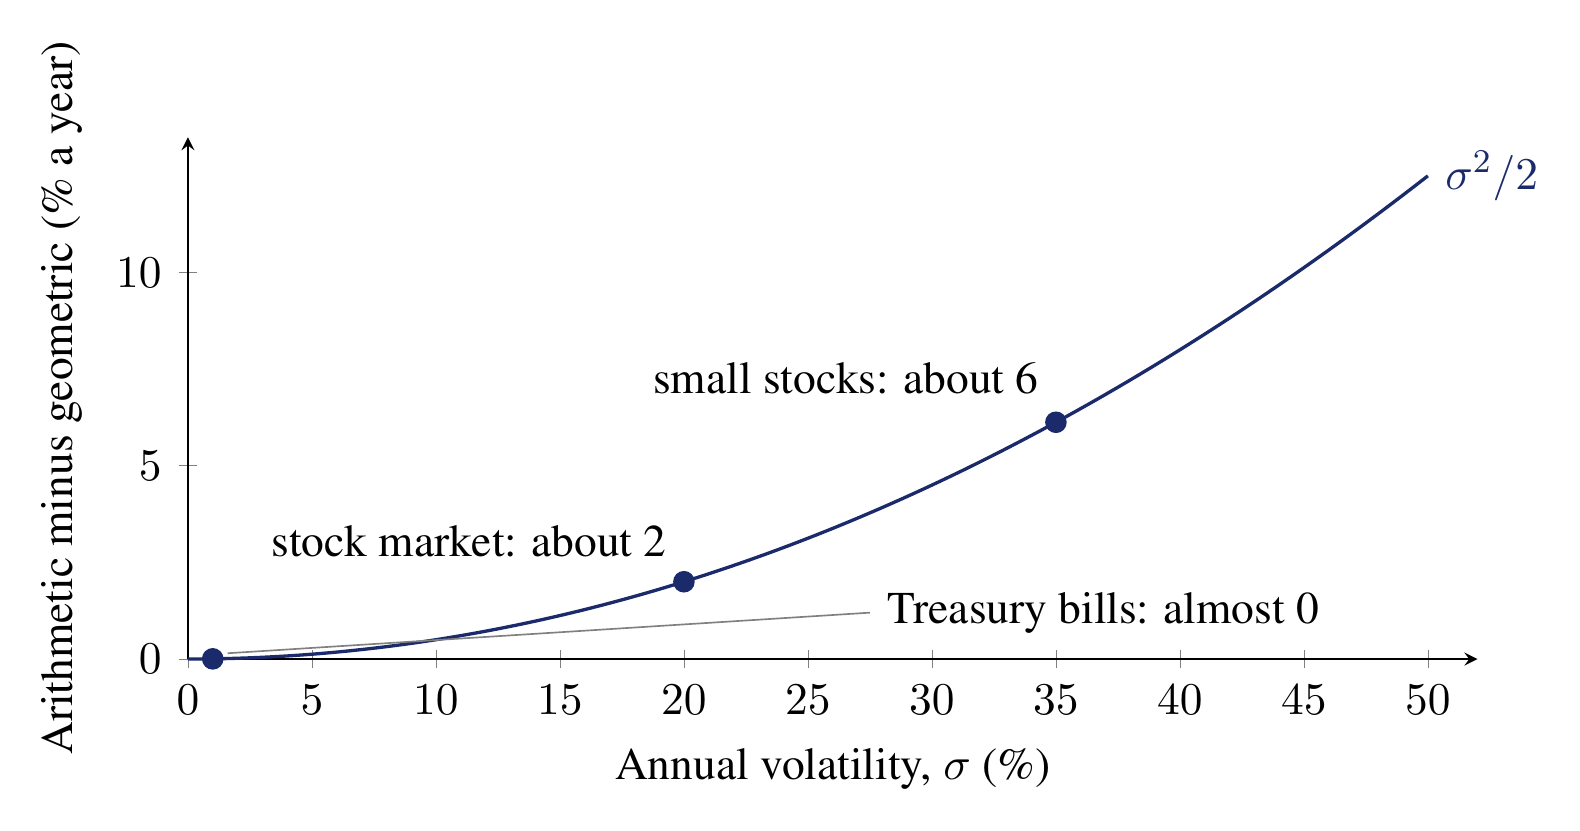
\includegraphics[width=0.85\linewidth]{images/fig02-1-volatility-drag.png}
%\caption{Volatility drag: the gap between the arithmetic and geometric average returns, from Equation~\eqref{eq:02-drag}. The gap is negligible for Treasury bills, about 2 percentage points a year for the stock market and about 6 for small stocks, and it rises with the square of volatility.}
%\label{fig:02-drag}
%\end{figure}


\providecolor{fenavy}{HTML}{1B2A6B}

\begin{figure}[!htbp]
  \centering
  \begin{tikzpicture}[
    % Arithmetic minus geometric mean = sigma^2 / 2.
    % With sigma in percent: (sigma/100)^2 / 2 * 100 = sigma^2 / 200 (% a year).
    declare function={gap(\s) = \s^2/200;}
  ]
  \begin{axis}[
    scale only axis, width=0.55\linewidth, height=0.28\linewidth,
    axis lines=left,
    axis line style={-stealth, thin},
    xmin=0, xmax=52, ymin=0, ymax=14,
    xtick={0,10,...,50},
    ytick={0,5,10},
    tick label style={font=\small},
    label style={font=\small},
    xlabel={Annual volatility, $\sigma$ (\%)},
    ylabel={Arith.\ minus geom.\ (\% a year)},
    samples=150, domain=0:50,
    clip=false,
  ]
    \addplot[fenavy, thick] {gap(x)};
    \node[fenavy, anchor=west, font=\small] at (axis cs:50.3,{gap(50)}) {$\sigma^2/2$};

    % Examples
    \fill[fenavy] (axis cs:1,{gap(1)})   circle (2pt);
    \fill[fenavy] (axis cs:20,{gap(20)}) circle (2pt);
    \fill[fenavy] (axis cs:35,{gap(35)}) circle (2pt);

    \node[anchor=south east, font=\footnotesize] at (axis cs:19.5,{gap(20)+0.2}) {stock market: about 2};
    \node[anchor=south east, font=\footnotesize] at (axis cs:34,{gap(35)+0.3}) {small stocks: about 6};
    \draw[gray!60] (axis cs:1.5,0.15) -- (axis cs:27,1.3);
    \node[anchor=west, font=\footnotesize] at (axis cs:27,1.4) {Treasury bills: almost 0};
  \end{axis}
  \end{tikzpicture}
  \caption{Volatility drag: the gap between the arithmetic and geometric average returns, from Equation~\eqref{eq:02-drag}. The gap is negligible for Treasury bills, about 2 percentage points a year for the stock market and about 6 for small stocks, and it rises with the square of volatility.}
  \label{fig:02-drag}
\end{figure}

\textbf{Implications:}
\begin{enumerate}
\item Use the arithmetic average when you need the expected return for a single period, as in the Sharpe ratio or a forecast, and use the geometric average when you report how much an investment grew. 
\item If you quote the arithmetic average as a growth rate, you will overstate what the investor experienced, and the overstatement is largest for the volatile strategies that tend to look most attractive. 
\item Whenever a source reports an average return, you should check which kind it is. Lab~\ref{ch:02} measures the gap on real portfolios.
\end{enumerate}

\section{Research datasets and their free alternatives}
\label{sec:02-datasets}

A result can be no more reliable than the data behind it. Each dataset covers different companies, periods and events, and each handles corrections, dividends and failed companies in its own way. 

Most published research on U.S. stocks rests on CRSP and Compustat, the two commercial databases introduced in Section~\ref{sec:02-foundations}. Two of their features\index{features and targets} matter most for this chapter, because free sources usually lack them.

\begin{itemize}
  \item \textbf{Delisting returns.}\index{return!delisting|textbf} CRSP includes companies that later disappeared, together with the return in the month in which each of them was delisted.
  \item \textbf{Point-in-time data.}\index{data!point-in-time|textbf} The point-in-time version of Compustat records what was known on each date, rather than the figures as they were later revised.
\end{itemize}

Many universities subscribe to these databases, but many readers will not have access to them. The labs in this book therefore use free sources that are either built from these databases or comparable to them:

\begin{center}
\small
\begin{tabularx}{0.9\linewidth}{@{}>{\raggedright\arraybackslash}p{0.22\linewidth}>{\raggedright\arraybackslash}X>{\raggedright\arraybackslash}p{0.26\linewidth}@{}}
\toprule
Free source & What it offers & Main limitation \\
\midrule
Kenneth R. French Data Library & Factor returns and portfolios sorted on size, value, momentum and more, built from CRSP and Compustat, since 1926 & Portfolio-level only; no individual stocks \\
FRED (Federal Reserve Bank of St.\ Louis) & Interest rates and economic series; its ALFRED archive keeps past vintages of revised data & Economic series, not stock-level data \\
Open Source Asset Pricing (Chen and Zimmermann) & Portfolio returns for over 200 published predictors & Full firm-level signals require WRDS \\
Jensen--Kelly--Pedersen global factors & 153 factors across 93 countries & Factor-level only \\
Yahoo Finance and similar & Daily prices for current stocks, ETFs and indexes & Mostly survivors only; adjustments not always documented; unofficial access methods can break \\
\bottomrule
\end{tabularx}
\end{center}

A \textbf{predictor}, also called a \textbf{signal}, is a variable that a study uses to forecast returns, such as a valuation ratio or a past return. The last row of the table deserves particular attention. Free stock-price sites are convenient, but they mostly cover companies that still exist today. A backtest that downloads today's stocks from such a site and runs them through the past therefore has survivorship bias built into it, which is the problem that Section~\ref{sec:02-survivorship} describes.

\section{Survivorship bias: the missing failures}
\label{sec:02-survivorship}

Companies that fail, merge or are delisted disappear from many datasets, and their final losses disappear with them. A backtest that is run only on companies that still exist never suffers those losses, so it overstates returns, often by several percentage points a year. This is one of the most common errors in practice, because most free price sources list only the stocks that trade today.

\subsection{Survivorship bias}

\textbf{Survivorship bias}\index{survivorship bias|textbf} arises when a sample includes only the companies, funds or strategies that are still around at the end of the period. Those that failed, were acquired or were shut down drop out of the data, and their losses drop out with them. It is like judging how safe a sport is by interviewing only the players who are still playing.

The bias works through three channels.

\begin{enumerate}
  \item \textbf{Survivors-only samples.} Testing a strategy on today's index members, or on the funds that exist today, removes every company or fund that failed along the way. The survivors are, by definition, the ones that did well enough to last.
  \item \textbf{Missing delisting returns.} When a stock leaves the exchange because the company is failing, its final return is often large and negative, and it is often missing from the database. Shumway (1997) showed that CRSP frequently lacked returns for delistings caused by poor performance, and he estimated that these missing returns averaged about $-30$\% for stocks on the NYSE and AMEX. Shumway and Warther (1999) found even larger losses for Nasdaq stocks. A backtest that silently drops these months overstates returns, and the error is largest for small and distressed stocks.
  \item \textbf{Backfill.}\index{backfill bias|textbf} Databases sometimes add a company or fund only after it has already succeeded, filling in its earlier history at the same time. This \textbf{backfill} brings in past returns only for those that did well. Kothari, Shanken and Sloan (1995) argued that this kind of selection in Compustat inflated the measured returns of high book-to-market\index{book-to-market ratio} stocks, which are companies whose accounting value is large relative to their market value.
\end{enumerate}

The bias is well documented for mutual funds. Elton, Gruber and Blake (1996) estimated that studying only the funds that survived overstated average performance by roughly 0.9 percentage points a year, which is large compared with the alphas\index{alpha} that researchers try to detect. Brown, Goetzmann, Ibbotson and Ross (1992) showed that survivorship can even make fund performance appear to persist from one period to the next when in fact it does not.

\subsection{The problem}

\textbf{Why survivorship can create a strategy out of nothing.} Survivorship bias does not simply shift all returns upward by the same amount. Its effect is strongest for the stocks that are most likely to fail, namely small, volatile and \textbf{distressed} companies that are at real risk of bankruptcy. Among such companies, the ones that survive are the ones whose prices happened to rise. As a result, a survivors-only backtest of a strategy that buys volatile or distressed stocks can show a large premium that is produced entirely by the way the sample was built. Lab~\ref{ch:02} demonstrates this with a simulation in which the true premium is known to be zero.

\subsection{The fix}

\textbf{The fix} is to use a dataset that includes failed companies and their delisting returns, such as CRSP, together with portfolio rules that use only the firms that were listed on each date. 
Most free sources in Section~\ref{sec:02-datasets} do not need this fix. The French library, Open Source Asset Pricing\index{Open Source Asset Pricing} and the Jensen--Kelly--Pedersen data are built from CRSP, so they include companies that later failed, and FRED\index{FRED} holds economic series rather than companies. The fix matters most for free stock-price sites such as Yahoo Finance, which list mainly today's survivors. Because those sites do not show which companies are missing, the Shumway correction cannot be applied, and the safer choice is to test the strategy on portfolio data that were built from a complete database.

When delisting returns are missing, researchers follow Shumway and substitute an estimate, such as $-30$\%.
Suppose a stock falls from \$10 to \$2 and is then delisted for poor performance, with no final return recorded.
If the final return is left blank, the backtest counts only the fall to \$2.
If the researcher follows Shumway, the backtest adds one more month with a $-30$\% return, as if the stock ended near \$1.40.
The estimate won’t be exact for any single company, but on average it is much closer to the truth than assuming a zero loss.
Do we need to do this fix? Probably not. Only researchers with stock-level data such as CRSP can apply it, because they can see which companies were delisted and which delisting returns are missing. Users of Yahoo Finance can’t, because the failed companies aren’t in the data at all.


\section{Look-ahead bias: using only what was known}
\label{sec:02-lookahead}

A backtest is honest only if every decision in it uses information that was available at the time. Accounting figures are published weeks or months after the period they describe, and economic data are often revised later. Using the final numbers as if they had been known in advance gives a strategy an advantage that no investor had, and the result can look excellent for no real reason.

\textbf{Look-ahead bias}\index{look-ahead bias|textbf} arises when a backtest uses information that was not yet available when the decision would have been made. It is easy to introduce and hard to notice, because the code runs without error and the results simply look better than they should. Figure~\ref{fig:02-timeline} shows the most common case, in which accounting data are used before they were published.

%\begin{figure}[htbp]
%\centering
%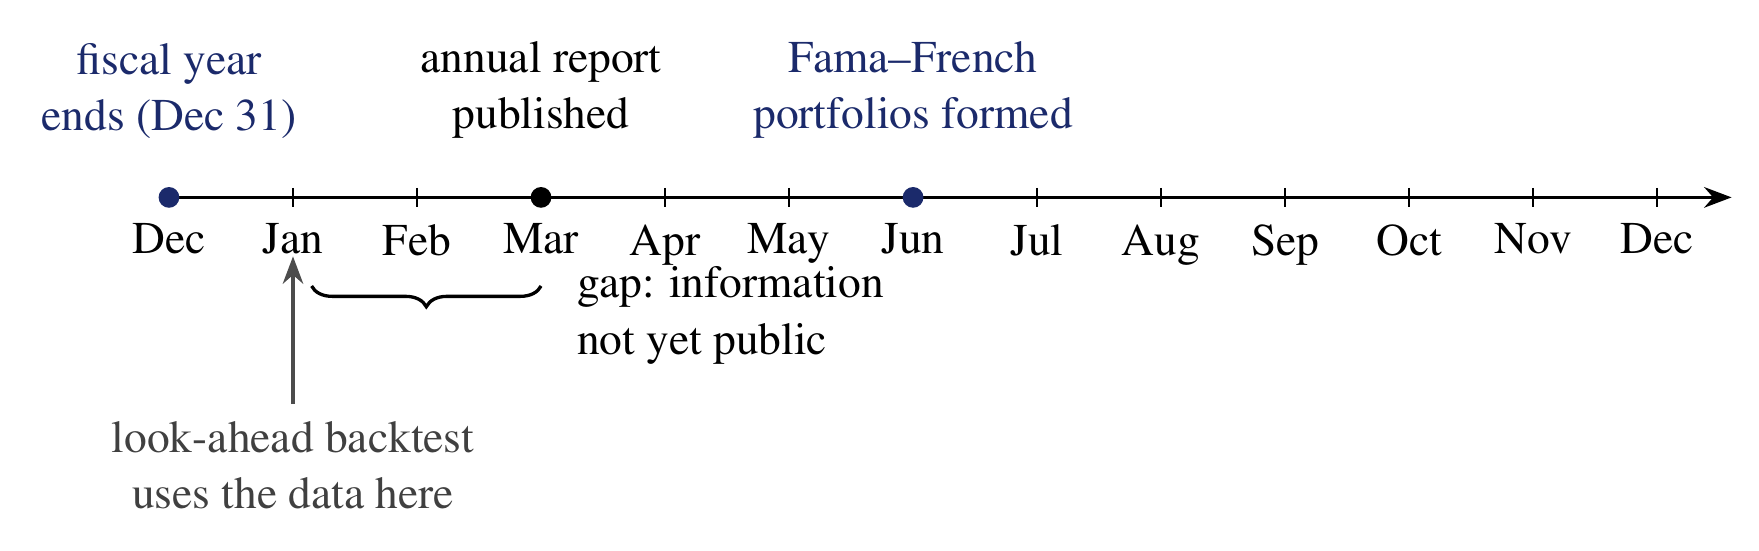
\includegraphics[width=0.9\linewidth]{images/fig02-2-accounting-timeline.png}
%\caption{When accounting data becomes usable. A company's fiscal year ends in December, but its annual report appears only months later. A backtest that trades on the figures in January uses information no investor had. Fama and French wait until the following June to be safe.}
%\label{fig:02-timeline}
%\end{figure}

\providecolor{fenavy}{HTML}{1B2A6B}
\providecolor{fegray}{HTML}{4D4D4D}

\begin{figure}[!htbp]
  \centering
  \begin{tikzpicture}[x=0.9cm, y=1cm, font=\small]
    % Timeline: Dec (0) to the following Dec (12)
    \draw[-stealth, thick] (0,0) -- (12.6,0);
    \foreach \wfI/\wfM in {0/Dec,1/Jan,2/Feb,3/Mar,4/Apr,5/May,6/Jun,
                           7/Jul,8/Aug,9/Sep,10/Oct,11/Nov,12/Dec} {
      \draw (\wfI,0.1) -- (\wfI,-0.1);
      \node[anchor=north] at (\wfI,-0.12) {\wfM};
    }

    % Key dates
    \fill[fenavy] (0,0) circle (2.6pt);
    \fill         (3,0) circle (2.6pt);
    \fill[fenavy] (6,0) circle (2.6pt);
    \node[fenavy, anchor=south, align=center] at (0,0.3)
      {fiscal year\\ends (Dec 31)};
    \node[anchor=south, align=center] at (3,0.3)
      {annual report\\published};
    \node[fenavy, anchor=south, align=center] at (6,0.3)
      {Fama--French\\portfolios formed};

    % Gap between fiscal year-end and publication
    \draw[decorate, decoration={brace, mirror, amplitude=5pt}]
      (1.1,-0.65) -- (2.9,-0.65);
    \node[anchor=north west, align=left] at (3.1,-0.5)
      {gap: information\\not yet public};

    % Look-ahead bias
    \draw[-stealth, fegray] (1,-1.9) -- (1,-0.6);
    \node[fegray, anchor=north, align=center] at (1,-2)
      {look-ahead backtest\\uses the data here};
  \end{tikzpicture}
\caption{When accounting data becomes usable. A company's fiscal year ends in December, but its annual report appears only months later. A backtest that trades on the figures in January uses information that no investor had, which is why Fama and French wait until the following June.}
\label{fig:02-timeline}
\end{figure}


The table below lists the common sources of look-ahead bias and the standard treatment against each.

\begin{center}
\small
\begin{tabularx}{0.9\linewidth}{@{}r>{\raggedright\arraybackslash}p{0.16\linewidth}>{\raggedright\arraybackslash}X>{\raggedright\arraybackslash}p{0.32\linewidth}@{}}
\toprule
 & Source & What goes wrong & Standard treatment \\
\midrule
1 & Same-period execution & A signal computed from today's closing price is used to trade at that same close & Trade on the next period's return: lag every signal by at least one period \\
2 & Accounting publication lags & Annual results for a December fiscal year are used in January, though they are published weeks or months later & Lag accounting data; Fama and French (1993) use fiscal-year data only from the following June \\
3 & Revised economic data & GDP or employment figures are used as revised years later, not as first reported & Use real-time vintages, such as FRED's ALFRED archive \\
4 & Index membership & Today's index members are used for the past & Use historical membership lists \\
5 & Full-sample choices & Parameters, thresholds or variable definitions are chosen using the whole sample, then ``tested'' on it & Choose using only data available at each date (walk-forward; Chapter~\ref{ch:08}) \\
6 & Full-sample scaling & Signals are standardized with means and volatilities computed over the whole sample & Use expanding or rolling estimates \\
\bottomrule
\end{tabularx}
\end{center}


Three terms in the table need explaining. To \textbf{lag} a signal is to use it only from a later period, so that it was already known before the trade. A \textbf{walk-forward}\index{walk-forward evaluation|textbf} test chooses its settings at each date using only the data available before that date, just as an investor in real time would have to. An \textbf{expanding} estimate uses all the data up to each date, whereas a \textbf{rolling} estimate uses a window of fixed length, such as the past five years.

The last two rows of the table describe the subtlest problems. In these cases no future price is used directly, yet the analyst's choices reflect knowledge of how the whole period turned out. For example, a trading rule whose window length was chosen because it worked best over 1926--2025 carries information from 2025 back into 1926.

\textbf{Point-in-time data}\index{data!point-in-time|textbf} is the general remedy, because it ensures that each date uses only the values that could have been known then. Lab~\ref{ch:02} measures two forms of look-ahead bias on real data, namely trading on the same day's closing price and choosing a rule's parameter with hindsight.

\section{Micro-caps: results no investor could capture}
\label{sec:02-microcaps}

The smallest companies are costly or impossible to trade in large amounts, yet in an equal-weighted portfolio they carry the same weight as the largest companies. A result can therefore be driven almost entirely by stocks that no investor could realistically buy. Checking how a portfolio is weighted, and whether its result survives without the smallest stocks, is one of the quickest ways to test whether a finding is usable.

The U.S. stock market is extremely unequal. A few hundred large companies account for most of its value, while thousands of tiny companies account for most of the names on the list. Fama and French (2008) classified stocks below the 20th percentile of NYSE market capitalization as \textbf{micro-caps}\index{micro-caps|textbf}, which means that each of them is smaller than four-fifths of the stocks listed on the New York Stock Exchange. They found that micro-caps made up about 60\% of all listed stocks but only about 3\% of total market value (Figure~\ref{fig:02-microcaps}).

%\begin{figure}[htbp]
%\centering
%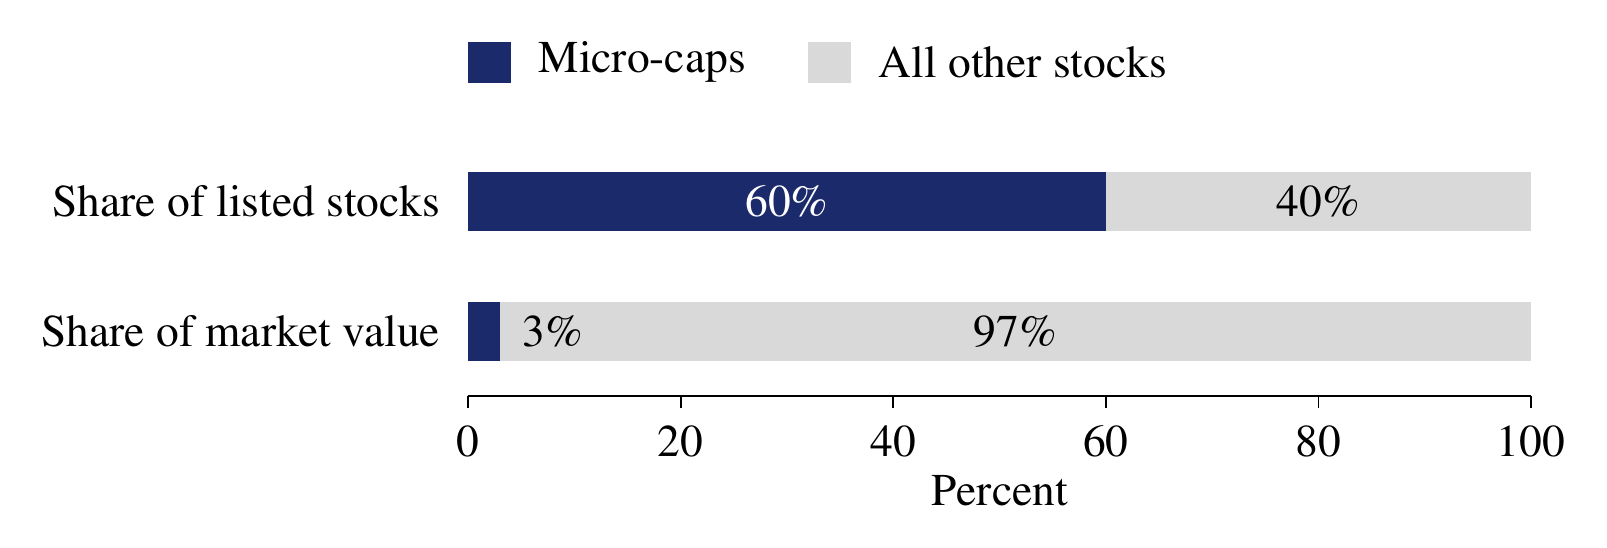
\includegraphics[width=0.8\linewidth]{images/fig02-3-microcaps.png}
%\caption{Micro-caps are most of the stocks but almost none of the money. Source: Fama and French (2008).}
%\label{fig:02-microcaps}
%\end{figure}


\providecolor{fenavy}{HTML}{1B2A6B}

\begin{figure}[!htbp]
  \centering
  \begin{tikzpicture}
  \begin{axis}[
    scale only axis, width=0.6\linewidth, height=2.4cm,
    xmin=0, xmax=100, ymin=0.4, ymax=2.6,
    axis x line*=bottom, axis y line=none,
    xtick={0,20,...,100},
    xlabel={Percent},
    xlabel style={yshift=4pt},
    clip=false,
  ]
    % Share of listed stocks: micro-caps 60%, others 40%
    \fill[fenavy]  (axis cs:0,1.7)  rectangle (axis cs:60,2.3);
    \fill[gray!25] (axis cs:60,1.7) rectangle (axis cs:100,2.3);
    \node[white] at (axis cs:30,2) {60\%};
    \node        at (axis cs:80,2) {40\%};

    % Share of market value: micro-caps 3%, others 97%
    \fill[fenavy]  (axis cs:0,0.7) rectangle (axis cs:3,1.3);
    \fill[gray!25] (axis cs:3,0.7) rectangle (axis cs:100,1.3);
    \node[anchor=west] at (axis cs:3.5,1) {3\%};
    \node              at (axis cs:51.5,1) {97\%};

    % Row labels
    \node[anchor=east] at (axis cs:-1,2) {Share of listed stocks};
    \node[anchor=east] at (axis cs:-1,1) {Share of market value};

    % Legend
    \fill[fenavy]  (axis cs:0,2.95)  rectangle (axis cs:4,3.25);
    \node[anchor=west] at (axis cs:5,3.1) {Micro-caps};
    \fill[gray!25] (axis cs:33,2.95) rectangle (axis cs:37,3.25);
    \node[anchor=west] at (axis cs:38,3.1) {All other stocks};
  \end{axis}
  \end{tikzpicture}
\caption{Micro-caps are most of the stocks but almost none of the money. Source: Fama and French (2008).}
\label{fig:02-microcaps}
\end{figure}


This matters because of the way portfolios are weighted (Section~\ref{sec:02-foundations}).

\begin{itemize}
  \item \textbf{Equal-weighted}\index{index weighting!equal-weighted|textbf} portfolios give every stock the same weight, so micro-caps dominate them simply because there are so many of them.
  \item \textbf{Value-weighted}\index{index weighting!value-weighted|textbf} portfolios weight stocks by market capitalization, so they reflect where investors' money actually is.
\end{itemize}

Micro-caps are also expensive and difficult to trade. Their \textbf{bid--ask spreads}\index{bid--ask spread|textbf}, the gap between the price at which you can buy and the price at which you can sell, are wide. They have little \textbf{liquidity}\index{liquidity|textbf}, which means that buying or selling even a modest amount moves the price. They are also costly to \textbf{sell short}\index{short selling|textbf}, that is, to borrow and sell in the hope of buying them back later at a lower price. In addition, micro-caps have the most extreme returns and the most data problems, including the missing delisting returns described in Section~\ref{sec:02-survivorship}. A pattern that appears in equal-weighted portfolios but not in value-weighted ones may therefore exist only where no large investor can exploit it.

The replication\index{replication} debate in Chapter~\ref{ch:07} turns partly on this point. An \textbf{anomaly}\index{anomaly|textbf} is a pattern in returns that standard risk models, such as the CAPM\index{capital asset pricing model (CAPM)}, cannot explain. Hou, Xue and Zhang\index{q-factor model} (2020) found that many anomalies disappear when micro-caps are given little weight, while their critics argue that this mainly shows that anomalies are concentrated among small stocks. Either way, the lesson for this chapter is simple: \textbf{always ask how a portfolio is weighted and whether the result survives without micro-caps.}

\begin{callout}
\textbf{What Failed: the size effect\index{size premium}.} Banz (1981) found that small companies had earned higher risk-adjusted returns than large ones, and ``small beats big'' became one of the best-known findings in finance. Later research, however, found that the effect became much weaker after it was published, that it was heavily concentrated among the very smallest stocks, and that in the early studies it was concentrated in January. Size remains a common factor in models of risk, but as a stand-alone source of extra return it has been far less reliable than its early evidence suggested. Lab~\ref{ch:02} tests how much of the size premium comes from micro-caps and how much comes from the years before 1981.
\end{callout}

\section{Data snooping: when a whole field searches one dataset}
\label{sec:02-snooping}

Chapter~\ref{ch:01} described the problem of selection within one researcher's search. There is a wider version of the same problem, in which an entire field searches the same data. Most research on U.S. stocks uses CRSP, and much of it uses the same period after 1963. Thousands of researchers have tested thousands of ideas on these data, and the ideas that ``worked'' were the ones that got published. Each paper may report a single, honest test, yet together the field has run an enormous number of trials on one history. A finding can therefore be a false discovery even when its author did nothing wrong, which is why a result must be confirmed on data that played no part in finding it.

Lo and MacKinlay (1990) called this \textbf{data-snooping bias}\index{data snooping|textbf}. When the choice of what to test is influenced by what earlier studies found in the same data, the usual significance levels\index{hypothesis testing!significance level} overstate the strength of the evidence. No single researcher can fix this bias, because no one knows how many ideas were tried and abandoned across the whole field.

Three defenses work, and later chapters use all of them.

\begin{enumerate}
  \item \textbf{New data.} Test the claim in periods or markets that played no part in its discovery, such as the years before the original sample, the years after publication, or other countries (Chapters~\ref{ch:06} and~\ref{ch:07}).
  \item \textbf{Higher hurdles.} Require stronger evidence for claims that are tested on heavily used data, such as a t-statistic\index{t-statistic} above 3 (Harvey, Liu and Zhu 2016; Chapter~\ref{ch:07}).
    \item \textbf{Economic reasoning stated in advance.} Before running a test, state why the pattern should exist. A story written after a pattern is found proves little, because a clever explanation can be invented for almost any result, including one produced by chance. A reason stated beforehand turns the test into a genuine check, because the data can prove it wrong. 
\end{enumerate}

\section{Lab~\thechapter: Four ways data can mislead}
\label{sec:02-lab}

\begin{callout}
\textbf{Lab~\ref{ch:02} at a glance.} \emph{Claim on trial:} free, public data can support a reliable backtest. \emph{Data:} monthly and daily U.S. market returns and size-sorted portfolios\index{portfolio sort} since 1926, from the Kenneth R. French Data Library\index{Kenneth French data library} (downloaded automatically), plus a simulated stock market. \emph{Tools:} Python with pandas, NumPy and matplotlib, plus the fintest module. \emph{Time:} about 90 minutes, including the guided notebook. \emph{Code:} repository folder \texttt{ch02-data-traps/}.
\end{callout}

The design of this lab draws on a line of well-known studies, each of which showed how one feature of the data can change a result. Brown, Goetzmann, Ibbotson and Ross (1992) used a simulation to show that dropping the funds that disappear can create patterns in performance that are not really there, and Shumway (1997) measured how large the missing delisting losses are. Brock, Lakonishok and LeBaron (1992) made moving-average trading rules famous, and Sullivan, Timmermann and White (1999) later showed how much of their apparent success came from searching across many rules. Banz (1981) discovered the size effect, and Horowitz, Loughran and Savin (2000) and Schwert (2003) found that it weakened after publication and depended heavily on the smallest stocks. Each part of the lab follows the logic of one of these studies, using free data, so that you can see the problem for yourself.

The lab measures each of the problems from Sections~\ref{sec:02-returns} to~\ref{sec:02-microcaps} in turn. Three of its parts use real data, while the part on survivorship uses a simulation. 
The reason for the simulation is itself part of the lesson. To measure survivorship bias, we need to compare a backtest on all companies, including the ones that failed, with the same backtest on the survivors alone. Free stock-price sites list mainly the companies that still exist, so the failures are missing. The French library does include failed companies, but only inside its portfolio returns, so we cannot take them out to see how much difference they make. A simulation solves this problem, because it gives us the full history of every company, including the ones that disappear.



\subsection*{Part A: Arithmetic versus geometric averages}

\textbf{Predict first.} Before running this part, write down which of the four portfolios you expect to show the largest gap between its arithmetic and geometric average returns, and roughly how large you expect that gap to be.

The lab computes both averages for Treasury bills, the stock market, and the largest and smallest 10\% of stocks, annualizing each in the same way so that the comparison is fair. It then compares each measured gap with the volatility-drag approximation from Section~\ref{sec:02-returns}, which says that the geometric average is roughly the arithmetic average minus half the variance\index{variance}, $G \approx A - \sigma^2/2$ (Lab Figure~\ref{ch:02}.1). You should expect almost no gap for Treasury bills, a gap of about 2 percentage points a year for the market, and the largest gap, several points a year, for the smallest stocks. If a measured gap differs from the approximation, ask why. The approximation assumes that returns are close to normally distributed, and the returns of small stocks are not.

\subsection*{Part B: Survivorship bias in a market where the truth is known}

\textbf{Predict first.} Before running this part, write down how much you expect survivorship bias to add to the market's average return each year.

With real data we never know the true answer, so the lab builds a market in which we do. This approach follows Brown, Goetzmann, Ibbotson and Ross (1992), who simulated funds with no skill and showed that keeping only the survivors made their performance appear to persist. The lab simulates about 2,000 listed companies over 30 years, and every company has the \textbf{same expected return}, so no stock or strategy has a real advantage. Following Shumway (1997), a company whose price falls below 20\% of its listing price is delisted with a final return of $-30$\%. Other companies are acquired at a premium, and every company that leaves is replaced by a new listing.

From this single simulated history, the lab builds three datasets:

\begin{center}
\small
\begin{tabularx}{0.9\linewidth}{@{}>{\raggedright\arraybackslash}p{0.26\linewidth}>{\raggedright\arraybackslash}X>{\raggedright\arraybackslash}p{0.28\linewidth}@{}}
\toprule
Dataset & What it contains & Real-world equivalent \\
\midrule
Full data & Every company, including its delisting return & CRSP, used correctly \\
Missing delisting returns & Every company, but without the final delisting month & A database with gaps in delisting returns \\
Survivors only & Only companies still listed at the end & Today's stocks downloaded from a free price site \\
\bottomrule
\end{tabularx}
\end{center}

On each dataset, the lab measures two things. The first is the equal-weighted market return. The second is the return of a strategy that each month buys the most volatile fifth of stocks and sells the least volatile fifth, where volatility is measured using past returns only (Lab Figure~\ref{ch:02}.2). The full data give the true answer, so any difference in the other two datasets comes entirely from the way they were built.

With the lab's default settings (2,000 listed companies, 30 years and seed 2026), 5,856 companies are listed over the period, 1,693 of them are delisted for poor performance, and 2,000 survive to the end. The results are as follows:

\begin{center}
\small
\begin{tabularx}{0.9\linewidth}{@{}>{\raggedright\arraybackslash}X>{\raggedright\arraybackslash}p{0.22\linewidth}>{\raggedright\arraybackslash}p{0.22\linewidth}r@{}}
\toprule
Dataset & Equal-weighted compound return & Volatile minus calm, per year & t-statistic \\
\midrule
Full data & 9.3\% & $-1.2$\% & $-2.2$ \\
Missing delisting returns & 10.7\% & $+2.0$\% & 3.5 \\
Survivors only & 14.0\% & $+12.0$\% & 14.7 \\
\bottomrule
\end{tabularx}
\end{center}

Read the table from top to bottom. In the full data, the volatile-minus-calm strategy loses about 1\% a year, because volatile companies are delisted more often. Leaving out only the delisting returns flips the sign, so that the strategy now appears to earn 2\% a year. Keeping only the survivors adds almost five percentage points a year to the market's return and creates a ``volatility premium'' of 12\% a year, with a t-statistic far beyond any hurdle in this book. None of this premium is real. Compare these numbers with your prediction.

\subsection*{Part C: Look-ahead bias}

\textbf{Predict first.} Before running this part, write down whether you expect a one-day timing error to change a strategy's Sharpe ratio a little or a lot.

\textbf{C1. Trading on the same day's close.} This part tests a classic timing rule, which holds stocks when the market closes above its 200-day \textbf{moving average}\index{moving average|textbf}, the average closing price over the past 200 trading days, and holds Treasury bills otherwise. Brock, Lakonishok and LeBaron (1992) studied rules of this kind on nearly a century of daily Dow Jones data and found that they appeared to predict returns. The lab runs the rule in two ways. The correct version makes its decision at yesterday's close and earns today's return, whereas the look-ahead version makes its decision at today's close but is still credited with today's return. The two versions differ by a single day, which is the kind of error that can hide in one misplaced line of code. Compare their returns and Sharpe ratios (Lab Figure~\ref{ch:02}.3).

\textbf{C2. Choosing the window with hindsight.} Next, the lab tests moving-average windows from 20 to 300 days and chooses one of them in two ways. The hindsight version picks the window with the best Sharpe ratio over the whole evaluation period. The walk-forward version picks, each January, the window that had worked best up to that point, using only past data (Lab Figure~\ref{ch:02}.4). The gap between the two versions measures how much a result is inflated by choosing a rule's settings after seeing the results. Sullivan, Timmermann and White (1999) made the same point on a much larger scale. They expanded the rules of Brock, Lakonishok and LeBaron to a universe of several thousand and adjusted for the search with a bootstrap\index{bootstrap}. The best rule still looked strong in the original sample, but it did not continue to outperform in the decade that followed.

\subsection*{Part D: Micro-caps, weighting and the size premium}

\textbf{Predict first.} Before running this part, write down whether you expect the size premium to be larger in value-weighted or in equal-weighted portfolios, and whether you expect it to survive after 1981.

Using size-sorted portfolios, the lab measures the \textbf{size premium}\index{size premium|textbf}, which is the return of the smallest tenth of stocks minus the return of the largest tenth. It does so in four ways, using value weights and equal weights, each with and without the smallest tenth of stocks. It then splits the sample into the years before and after Banz published his finding in 1981 (Lab Figure~\ref{ch:02}.5). Together, these steps test the What Failed box in Section~\ref{sec:02-microcaps} directly. They also repeat, with free data, two tests from the literature. Horowitz, Loughran and Savin (2000) found that removing the very smallest firms eliminated any statistically significant\index{statistical significance} size effect, and Schwert (2003) found that the size effect weakened after the papers that reported it were published. If the premium lives mainly in tiny, hard-to-trade stocks, or if it disappeared after it was published, the claim weakens.

\emph{[Draft note: figures and numbers for Parts A, C and D are generated from the Kenneth R. French data at the time of publication; the book prints those results. The Part B simulation is fixed by design and its results can be printed as they stand.]}

\section{Verdict}
\label{sec:02-verdict}

Readers write one sentence for each problem, saying how much it changed the result and in which direction, and then judge the claim. The expected verdict is \textbf{survives, with conditions}. Free data can support a reliable backtest when you do the following:

\begin{enumerate}
  \item use total returns, compare them with a total-return benchmark, and quote the geometric average when reporting growth (Part A);
  \item use data that include failed companies, such as the French library's portfolios, which are built from CRSP, rather than a list of today's stocks (Part B);
  \item lag every signal and every accounting figure, and choose a rule's settings with walk-forward tests (Part C);
  \item check that the result survives value weighting and the removal of micro-caps (Part D).
\end{enumerate}

A backtest that skips these steps can look excellent and still mean nothing, while one that follows them can be trusted as far as its statistics allow. The checklist in the next section turns these conditions into questions that you can ask of any backtest, including your own.

\section{What investors can use}
\label{sec:02-checklist}

Before you trust any backtest, whether it is your own or someone else's, work through the following questions. Each question corresponds to a section of this chapter, and most of them can be answered in a few minutes.

\begin{itemize}
  \item[$\square$] \textbf{Returns (Section~\ref{sec:02-returns}):} Are the returns total returns that include dividends? Are they compared with a total-return benchmark? Is the reported average arithmetic or geometric?
  \item[$\square$] \textbf{Excess returns (Section~\ref{sec:02-returns}):} Is performance measured above the risk-free rate?
  \item[$\square$] \textbf{Survivorship (Section~\ref{sec:02-survivorship}):} Does the dataset include companies or funds that no longer exist, and are their delisting returns included?
  \item[$\square$] \textbf{Look-ahead (Section~\ref{sec:02-lookahead}):} Is every signal lagged so that it uses only information available before the trade, and are accounting data lagged to their publication dates?
  \item[$\square$] \textbf{Hindsight choices (Section~\ref{sec:02-lookahead}):} Were any parameters, thresholds or universes chosen using the whole sample?
  \item[$\square$] \textbf{Weighting (Section~\ref{sec:02-microcaps}):} Is the portfolio value-weighted or equal-weighted, and does the result survive without micro-caps?
  \item[$\square$] \textbf{Shared data (Section~\ref{sec:02-snooping}):} Has the result been tested on data that played no part in its discovery, such as other periods, other markets or the years after publication?
\end{itemize}

\textbf{Questions to ask a fund manager or strategy vendor}

\begin{itemize}
  \item Which database was the backtest built on, and does it include delisted stocks and their delisting returns?
  \item How were the signals lagged, and when would each piece of data actually have been available?
  \item Is the strategy value-weighted or equal-weighted, and what share of its return comes from the smallest stocks?
  \item Is the reported return an arithmetic or a compound average, and is it measured before or after costs?
\end{itemize}

\section*{Exercises}

\subsection*{Conceptual (all readers)}

\begin{enumerate}
  \item A strategy reports an average annual return of 18\% with a volatility of 40\%. Estimate its geometric average. Which number should an investor care about, and why?
  \item Explain why a portfolio's simple return is a weighted average of the simple returns of its holdings, while a multi-period return is a sum of log returns.
  \item A researcher backtests a strategy from 2005 to today on the stocks that are in the S\&P 500 index today. Name two biases in this design and the direction of each.
  \item A study uses annual accounting data for fiscal years ending in December and forms portfolios in January of the next year. What is the problem, and how do Fama and French avoid it?
  \item Explain why survivorship bias can create a premium for volatile stocks, rather than simply raising all returns by the same amount.
  \item A paper reports a strong anomaly in equal-weighted portfolios that disappears in value-weighted ones. What does this suggest about who could profit from it?
\end{enumerate}

\subsection*{Lab extensions (technical readers)}

\begin{enumerate}
  \setcounter{enumi}{6}
  \item Re-run Part B with a delisting return of $-55$\%, which is closer to the estimates for Nasdaq stocks. How do the three datasets change?
  \item In Part C, try windows of 50 and 300 days. Is the look-ahead gain larger for fast rules or for slow ones? Explain why.
  \item In Part C, charge a trading cost of 0.1\% each time the rule switches. Does the correctly traded rule still beat buy-and-hold on a risk-adjusted basis?
  \item In Part D, move the publication split to 1990 and then to 2000. When does the size premium appear to fade?
  \item \textbf{Challenge:} Using a free price source, backtest an equal-weighted portfolio of today's S\&P 500 members over the past 20 years and compare it with the equal-weighted S\&P 500 index. Which problem from this chapter explains the difference?
\end{enumerate}
   % 2  Claim: Historical Data Show What a Strategy Would Have Earned

% ---- Part II: Regression, factor models and the cross-section
\part{Factor Models and the Cross-Section}
% Chapter 3 -- Claim: Size and Value Explain Returns That Beta Cannot (was Ch. 3)
% Figures need tikz and pgfplots (with the fillbetween library) in the preamble.
\providecolor{fenavy}{HTML}{1B2A6B}
\providecolor{fegray}{HTML}{4D4D4D}

\chapter{Claim: Size and Value Explain Returns That Beta Cannot}
\label{ch:03}

The Capital Asset Pricing Model (CAPM) provides a foundational answer to a central question in finance: why should assets with different risk characteristics earn different expected returns? In its standard form, the CAPM predicts that expected excess returns are proportional to market beta. Once beta is taken into account, firm characteristics such as size, valuation ratios, profitability, and investment should not provide additional information about expected returns. This implication makes the model empirically testable: if portfolios with different characteristics continue to earn different average returns after controlling for market exposure, the single-factor model is incomplete.

Early empirical studies found evidence of a positive relation between market beta and average returns, although the strength of that relation was not always consistent with the CAPM's predictions (Black, Jensen, and Scholes 1972; Fama and MacBeth 1973). Later studies documented return patterns associated with firm characteristics. Basu (1977) found that stocks with low price--earnings ratios earned higher returns than the CAPM would predict. Banz (1981) documented a size effect, while Rosenberg, Reid, and Lanstein (1985) reported higher returns for stocks with high book-to-market ratios. These findings raised a basic question: could market beta alone explain the cross-section of average stock returns?

Fama (1970) emphasized that tests of market efficiency are joint tests of market efficiency and the model used to measure expected returns. An apparent return anomaly may therefore indicate either market mispricing or an incomplete asset-pricing model. Fama and French (1992) showed that size and book-to-market equity helped explain differences in average returns that market beta did not adequately explain in their sample. They subsequently developed a three-factor model incorporating the market, size, and value factors (Fama and French 1993). Later work extended this framework by adding profitability and investment (Fama and French 2015). These models became influential tools for describing portfolio returns and evaluating investment performance.

The economic interpretation of these return patterns remains debated. A risk-based interpretation views size and value factors as proxies for common sources of risk for which investors require compensation. A behavioral interpretation argues that some premiums arise because investors extrapolate past growth, overreact to disappointing news, or misprice firms (Lakonishok, Shleifer, and Vishny 1994). The same empirical pattern can therefore be consistent with different explanations. A factor model can describe return differences without, by itself, establishing why those differences exist.

Multifactor models also have practical consequences. They affect how investors distinguish manager skill from exposure to systematic factors, how researchers evaluate fund performance, and how companies estimate the cost of equity (Graham and Harvey 2001). At the same time, the proliferation of proposed factors creates a statistical challenge. Harvey, Liu, and Zhu (2016) catalogued 316 factors across 313 published works and selected working papers, while noting that the number of factors actually tested was likely larger because unsuccessful experiments often remain unpublished. Their analysis argues that newly proposed factors should face a more demanding statistical hurdle than the conventional threshold of approximately 2.

The claim examined in this chapter is therefore: \textbf{size and value factors help explain differences in portfolio returns that the CAPM does not adequately explain, but the search for additional factors creates a multiple-testing problem that requires stronger statistical evidence.}

The chapter develops this argument in three stages. First, it reviews the statistical foundations needed to describe return distributions and interpret linear regressions. Second, it traces the development from the CAPM to the Fama--French three- and five-factor models, considers competing explanations for factor premiums, and examines the factor zoo and the multiple-testing problem. Third, the lab compares the CAPM and the Fama--French three-factor model using the 25 portfolios formed on size and book-to-market, then uses a controlled simulation to illustrate how testing many candidate factors can generate false discoveries.

By the end of the chapter you will be able to:
\begin{itemize}
  \item describe return distributions using the mean, variance, skewness, kurtosis, and autocorrelation, and interpret a basic linear regression;
  \item distinguish systematic risk from idiosyncratic risk and explain the role of beta in the CAPM;
  \item explain how the Fama--French three- and five-factor models extend the CAPM, and interpret alpha and factor loadings;
  \item describe the economic interpretations of size, value, profitability, and investment premiums, including the distinction between risk-based and behavioral explanations;
  \item explain why testing many candidate factors increases the probability of false discoveries;
  \item summarize the main findings of Harvey, Liu, and Zhu (2016), including their recommendation that newly discovered factors generally require a $t$-statistic greater than 3.0;
  \item distinguish statistical significance from economic significance and identify practical considerations that affect the implementation of factor strategies.
\end{itemize}

In the lab, you will estimate the CAPM and the Fama--French three-factor model for the 25 size-and-book-to-market portfolios, compare their explanatory performance, and conduct a simulation in which all candidate factors have known zero premiums.

\section{Foundations: distributions and regression}
\label{sec:03-foundations}

This section reviews two tools used throughout empirical asset pricing: summary statistics for return distributions and linear regression. Readers familiar with these methods may skim the section, but the notation and distinctions introduced here will be useful in the model comparisons that follow.

\subsection{Describing a distribution}
Four commonly used statistical moments summarize important features of a return distribution:
\begin{itemize}
  \item The \textbf{mean}\index{mean} is its center: the average return.
  \item The \textbf{variance}\index{variance|textbf}, or its square root, the standard deviation\index{standard deviation}, measures spread: how far returns typically fall from the mean.
  \item \textbf{Skewness}\index{skewness|textbf} measures asymmetry around the mean. Negative skewness indicates a longer or heavier left tail, so unusually large losses are more prominent than unusually large gains.
  \item \textbf{Kurtosis}\index{kurtosis|textbf} measures the weight of a distribution's tails relative to a normal distribution. A normal distribution has kurtosis 3; a value above 3 implies positive excess kurtosis and indicates greater weight in the tails.
\end{itemize}

Figure~\ref{fig:03-moments} illustrates how each moment changes the shape of a distribution. The mean and variance describe its center and spread, while skewness and kurtosis describe features that a mean--variance summary can miss. Two portfolios can have the same average return and standard deviation but very different probabilities of extreme losses.

\begin{figure}[htbp]
\centering
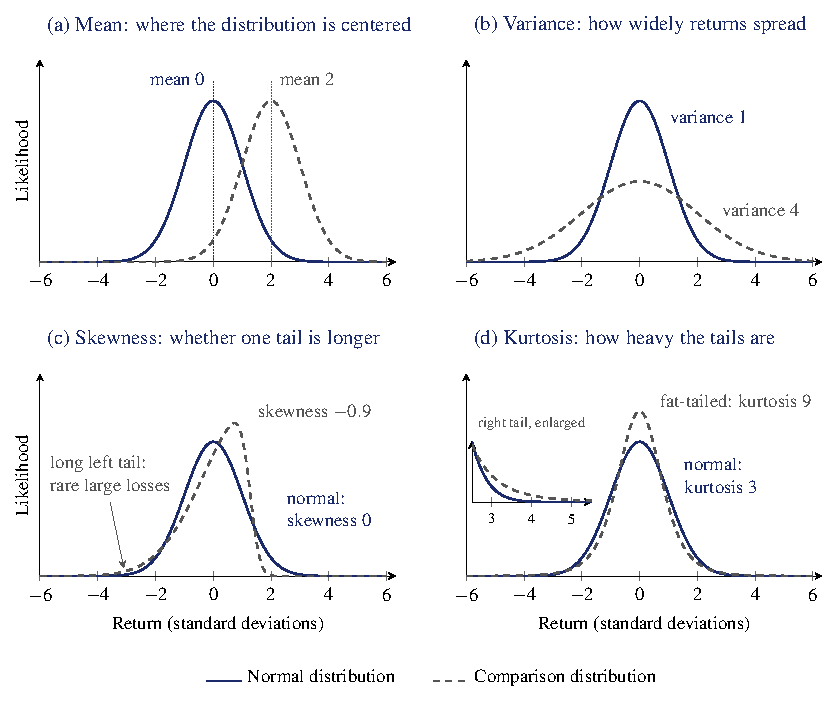
\includegraphics[width=0.7\linewidth]{images/fig03-0-moments.pdf}
\caption{The four moments of a distribution. Each panel compares the standard normal distribution (solid) with one that differs in a single respect. (a)~The mean sets the center. (b)~The variance sets the spread. (c)~Negative skewness lengthens the left tail, so large losses are more likely than large gains of the same size. (d)~Higher kurtosis puts more weight in the tails: the normal distribution has kurtosis 3, the fat-tailed one shown has kurtosis 9. Panels (c) and (d) keep the mean and variance of the normal distribution.}
\label{fig:03-moments}
\end{figure}

A fifth measure describes dependence over time. \textbf{Autocorrelation}\index{autocorrelation|textbf} is the correlation between a series and its own lagged values. The first-order autocorrelation ($\rho_1$) compares each month's return with the previous month's return. A value near $+1$ indicates strong positive linear dependence; a value near $-1$ indicates strong negative linear dependence; and a value near zero indicates little linear dependence at that lag. Zero autocorrelation does not rule out every form of predictability: nonlinear patterns or dependence at other lags may still be present.

\subsection{Linear regression and ordinary least squares}
\label{sec:03-regression}
A regression summarizes the linear relationship between a dependent variable, $y$, and an explanatory variable, $x$. Ordinary least squares\index{regression!ordinary least squares (OLS)} (OLS) estimates
\begin{equation}
  y_t = \alpha + \beta x_t + \varepsilon_t
  \label{eq:03-ols}
\end{equation}
by choosing the intercept $\alpha$ and slope $\beta$ to minimize the sum of squared residuals, $\sum_t \varepsilon_t^2$. The \textbf{residuals}\index{regression!residuals|textbf} are the differences between observed and fitted values. The slope measures the fitted change in $y$ associated with a one-unit change in $x$; the intercept is the fitted value of $y$ when $x=0$. For an in-sample regression with an intercept, the $R$-squared\index{regression!R-squared@$R^2$|textbf} ($R^2$) measures the fraction of the sample variation in $y$ accounted for by the fitted regression, ranging from 0 to 1. A high $R^2$ describes goodness of fit; it does not establish causation or prove that the model is economically correct.


% =====================================================================
% PART ONE OF THE CHAPTER: THE DEVELOPMENT OF RISK DECOMPOSITION
% =====================================================================
\section{Risk and expected return}
\label{sec:03-decomposition}


Asset-pricing models seek to explain differences in expected returns through investors' exposure to systematic risks. The CAPM begins with a single market factor, but empirical studies have identified return patterns associated with size, book-to-market equity, profitability, and investment. This section examines how multifactor models extend the CAPM and why the economic interpretation of their additional factors remains an important question.


\subsection{The CAPM: one source of priced risk}
\label{sec:03-capm}
The Capital Asset Pricing Model\index{capital asset pricing model (CAPM)} (Sharpe 1964; Lintner 1965; Mossin 1966) is a foundational equilibrium model of the relationship between risk and expected return. It distinguishes between two broad components of risk. \textbf{Systematic risk}\index{risk!systematic|textbf} reflects common movements in the market and cannot be eliminated through diversification. \textbf{Idiosyncratic risk}\index{risk!idiosyncratic|textbf} is specific to an individual asset or firm and can be reduced by holding a diversified portfolio. Under the CAPM's assumptions, investors are compensated for bearing systematic risk, not for bearing diversifiable, firm-specific risk.

In the CAPM equilibrium, investors combine the risk-free asset with the market portfolio. An asset's relevant risk is therefore measured by its contribution to the risk of that market portfolio. Beta summarizes this sensitivity: it measures how strongly the asset's return tends to move with the market, rather than measuring the asset's total volatility.


The CAPM has had a lasting influence on both research and practice. Companies use it to estimate the cost of equity and the discount rate\index{discount rate} for investment projects; a survey by Graham and Harvey (2001) found that the CAPM was widely used by chief financial officers. The model also provides a benchmark for performance evaluation: alpha is the part of a portfolio's return not explained by its exposure to the market factor. The CAPM's prediction that the market portfolio is the common risky portfolio also provides an important theoretical rationale for broad market-index investing.

Formally, the CAPM says that an asset's expected excess return\index{return!excess} is proportional to its \textbf{beta}\index{beta|textbf}, its sensitivity to the market:
\begin{equation}
  E[R^{e}_{i}] = \beta_i \, E[R^{e}_{m}], \qquad \beta_i = \frac{\operatorname{Cov}(R_i, R_m)}{\operatorname{Var}(R_m)}
  \label{eq:03-capm}
\end{equation}
Here $R_i$ is the asset's return, $R_m$ is the market return, and $R_f$ is the risk-free rate. Thus, $R^{e}_{i}=R_i-R_f$ and $R^{e}_{m}=R_m-R_f$ are the corresponding excess returns, as in Equation~\eqref{eq:excess-return}. Covariance measures how two returns move together, while variance measures the dispersion of one return series. A beta of 1.5 means that, on average in the estimated linear relationship, a 1\% change in the market's excess return is associated with a 1.5\% change in the asset's excess return. It does not mean that the asset will move by exactly 1.5\% in every period.

The regression model is estimated in time series:
\begin{equation}
  R^{e}_{i,t} = \alpha_i + \beta_i R^{e}_{m,t} + \varepsilon_{i,t}
  \label{eq:03-capm-ts}
\end{equation}
This is Equation~\eqref{eq:03-ols} with the asset's excess return as $y$ and the market's excess return as $x$. The slope $\beta_i$ measures the asset's market exposure. The intercept $\alpha_i$\index{alpha|textbf} (alpha) is the average return not explained by that exposure. The CAPM predicts that the population alpha is zero. An estimated positive alpha is not, by itself, proof of investment skill: it may reflect sampling uncertainty, omitted risk factors, model misspecification, or genuine abnormal performance. Figure~\ref{fig:03-alpha} illustrates the intercept and slope.

\begin{figure}[!htbp]
  \centering
  \begin{tikzpicture}[
    % Fitted regression: strategy = 1.16 + 1.15 * market
    declare function={fit(\x) = 1.16 + 1.15*\x;  zero(\x) = 1.15*\x;}
  ]
  \begin{axis}[
    scale only axis, width=0.41\linewidth, height=0.29\linewidth,
    axis lines=left,
    axis line style={-stealth, thin},
    xmin=-11, xmax=12.5, ymin=-12.5, ymax=16,
    xtick={-8,-4,0,4,8,12},
    ytick={-10,-5,0,5,10,15},
    tick label style={font=\footnotesize}, label style={font=\small},
    xlabel={Market excess return, $R^{e}_{m}$ (\% a month)},
    ylabel={Strategy excess return (\%)},
    clip=false,
  ]
    % Reference axes through zero
    \draw[gray!40] (axis cs:-11,0) -- (axis cs:12.5,0);
    \draw[gray!40] (axis cs:0,-12.5) -- (axis cs:0,16);

    % Monthly observations (illustrative)
    \addplot[only marks, mark=*, mark size=1.6pt, gray!60] coordinates {
      (0.51,2.80) (1.75,3.22) (-0.65,1.41) (-3.24,-0.57) (-1.41,-1.36)
      (-3.66,-2.80) (0.75,1.49) (6.13,8.66) (-1.57,-2.27) (-2.11,-2.05)
      (2.56,3.99) (2.00,4.86) (0.94,3.96) (-3.41,-4.63) (0.38,0.58)
      (3.42,6.19) (-5.15,-7.62) (-1.42,-1.08) (-7.49,-7.73) (-4.92,-2.80)
      (-7.24,-6.33) (-0.49,0.21) (-4.82,-4.97) (1.64,2.83) (1.16,4.75)
      (-0.29,0.31) (-10.07,-11.07) (-1.76,-0.34) (0.30,1.43) (0.98,2.12)
      (-5.93,-7.31) (-1.51,-0.55) (-3.61,-3.64) (-2.90,-0.54) (4.96,8.01)
      (-2.89,-2.20) (0.36,2.61) (4.21,5.75) (-1.95,0.41) (0.03,1.27)
      (0.96,3.20) (0.77,0.35) (-4.65,-3.75) (0.82,-0.15) (6.21,5.73)
      (-6.00,-6.26) (4.11,4.84) (1.00,2.66) (-2.19,1.80) (8.90,10.59)
      (3.70,4.74) (-4.54,-3.82) (0.81,2.90) (2.92,4.45) (-0.29,0.61)
    };

    % Zero-alpha line and fitted line
    \addplot[thick, dashed, fegray, domain=-11:12, samples=2] {zero(x)};
    \addplot[very thick, fenavy, domain=-11:12, samples=2] {fit(x)};
    \node[fenavy, anchor=west, font=\footnotesize] at (axis cs:12.3,{fit(12)+0.5}) {fitted line};
    \node[fegray, anchor=west, font=\footnotesize] at (axis cs:12.3,{fit(12)-3.5}) {zero-alpha line};

    % Slope triangle: run 3, rise 3 x beta
    \draw[fenavy] (axis cs:6,{fit(6)}) -- (axis cs:9,{fit(6)}) -- (axis cs:9,{fit(9)});
    \node[fenavy, anchor=north, font=\footnotesize] at (axis cs:7.5,{fit(6)-0.2}) {3};
    \node[fenavy, anchor=north west, font=\footnotesize, align=left] at (axis cs:9.3,{fit(6)-0.3})
      {rise $= 3\times$ beta\\beta $= 1.15$};

    % Alpha: the fitted line's value at a zero market return
    \fill[fenavy] (axis cs:0,1.16) circle (2.6pt);
    \draw[-stealth, fenavy] (axis cs:5.6,-3.4) -- (axis cs:0.4,0.9);
    \node[fenavy, anchor=north west, align=left, font=\footnotesize] at (axis cs:5.6,-2.6)
      {alpha $= 1.16$: the fitted line's\\value when the market return is 0};
  \end{axis}
  \end{tikzpicture}
\caption{Beta and alpha in a regression of a strategy's monthly excess returns on the market's. Beta is the slope of the fitted line; alpha is its height where the market's excess return is zero, the gap between the fitted line and a line with the same slope through the origin. Simulated data, with an alpha larger than any real strategy's so that it is visible.}
\label{fig:03-alpha}
\end{figure}

\textbf{The CAPM's variance decomposition.} The regression also provides a useful decomposition of return variance. In an OLS regression with an intercept, the fitted component is orthogonal to the residuals in the estimation sample. The sample variance can therefore be written as the sum of the variance explained by the market component and the residual variance:
\begin{equation}
  \operatorname{Var}(R^{e}_{i}) = \beta_i^2 \operatorname{Var}(R^{e}_{m}) + \operatorname{Var}(\varepsilon_i)
  \label{eq:03-vardec-capm}
\end{equation}

Let's understand the two terms:
\begin{enumerate}
\item The first term is the \textbf{systematic variance}\index{variance!systematic|textbf}, the part that comes from exposure to the market, and 
\item the second is the \textbf{idiosyncratic variance}\index{variance!idiosyncratic|textbf}, the part that belongs to the asset alone. 
\end{enumerate}
In this single-factor regression, the ratio of the fitted market component's variance to total return variance equals the in-sample $R^2$. Thus, an $R^2$ of 0.90 means that 90\% of the sample variance is associated with the fitted market component and 10\% remains in the residuals. This is a statement about variance in the sample, not a claim that the market causes 90\% of the asset's risk in every setting.

\begin{figure}[!htbp]
  \centering
  \begin{tikzpicture}[x=1cm, y=0.05cm]
    % Vertical axis: share of total variance, 0 to 100 percent
    \draw[-stealth, thin] (0,0) -- (0,108);
    \foreach \vdY in {0,50,100} {
      \draw (-0.08,\vdY) -- (0.08,\vdY);
      \node[anchor=east, font=\footnotesize] at (-0.1,\vdY) {\vdY};
    }
    \node[rotate=90, font=\small] at (-1.0,50) {Share of total variance (\%)};
    \draw[thin] (0,0) -- (6.6,0);

    % Bar 1: one stock, 31% systematic and 69% idiosyncratic
    \fill[fenavy!75] (0.8,0) rectangle (2.6,31);
    \fill[fenavy!15] (0.8,31) rectangle (2.6,100);
    \draw[fenavy] (0.8,0) rectangle (2.6,100);
    \node[white, font=\footnotesize, align=center] at (1.7,15.5) {systematic\\31\%};
    \node[fenavy, font=\footnotesize, align=center] at (1.7,65.5) {idiosyncratic\\69\%};
    \node[anchor=north, font=\small, align=center] at (1.7,-2) {One stock};

    % Bar 2: portfolio of 100 stocks, 98% systematic and 2% idiosyncratic
    \fill[fenavy!75] (3.8,0) rectangle (5.6,98);
    \fill[fenavy!15] (3.8,98) rectangle (5.6,100);
    \draw[fenavy] (3.8,0) rectangle (5.6,100);
    \node[white, font=\footnotesize, align=center] at (4.7,49) {systematic\\98\%};
    \draw[fenavy, thin] (5.6,99) -- (6.0,104);
    \node[fenavy, anchor=west, font=\footnotesize] at (6.0,104) {idiosyncratic 2\%};
    \node[anchor=north, font=\small, align=center] at (4.7,-2) {Portfolio of\\100 stocks};
  \end{tikzpicture}
  \caption{Splitting total variance into systematic and idiosyncratic parts with Equation~\eqref{eq:03-vardec-capm}. Each stock has a market beta of 1.2 and a residual standard deviation of 8\% a month, and the market's standard deviation is 4.5\% a month. Diversification leaves the systematic variance unchanged but divides the idiosyncratic variance by 100, so the systematic share, which equals the regression's $R^2$, rises from about 31\% to about 98\%. The numbers are illustrative.}
  \label{fig:03-vardec}
\end{figure}

The CAPM implies that a stock's expected return depends not on its total volatility, but on how sensitive it is to movements in the overall market. In practice, the CAPM provides a benchmark for determining the required return on investments, estimating the cost of equity capital for companies, evaluating portfolio performance, and making capital budgeting decisions. 

Empirical tests have found that the CAPM does not fully describe the cross-section of average returns. Under the model, average excess returns should lie on a straight line relating expected return to beta, known as the \textbf{security market line}\index{security market line|textbf}. Black, Jensen, and Scholes (1972) found a flatter relation than the CAPM predicts: low-beta portfolios earned more, and high-beta portfolios less, than their estimated betas implied (Figure~\ref{fig:03-sml}). This evidence challenges the view that market beta alone is sufficient to explain differences in average returns. 

Fama and French (1992) provided further evidence that firm size and the book-to-market ratio\index{book-to-market ratio} help explain the cross-section of average returns beyond market beta. The CAPM remains an important benchmark, but these findings motivated models that include additional factors. Importantly, a characteristic that helps explain average returns is not automatically a distinct source of systematic risk; that interpretation requires further economic argument and evidence.




\begin{figure}[!htbp]
  \centering
  \begin{tikzpicture}[
    % CAPM security market line: E[R^e] = 8 * beta (% a year)
    % Illustrative empirical line, flatter: 3 + 3.5 * beta
    declare function={sml(\b) = 8*\b; emp(\b) = 3 + 3.5*\b;}
  ]
  \begin{axis}[
    scale only axis, width=0.43\linewidth, height=0.28\linewidth,
    axis lines=left,
    axis line style={-stealth, thin},
    xmin=0, xmax=1.95, ymin=0, ymax=15.5,
    xtick={0,0.5,1,1.5},
    ytick={0,4,8,12},
    xticklabel style={/pgf/number format/fixed},
    tick label style={font=\small}, label style={font=\small},
    xlabel={Beta, $\beta$},
    ylabel={Average excess return (\% a year)},
    clip=false,
  ]
    % CAPM prediction
    \addplot[fenavy, very thick, domain=0:1.85, samples=2] {sml(x)};
    \node[fenavy, anchor=west, font=\footnotesize] at (axis cs:1.86,{sml(1.85)}) {CAPM prediction};

    % Flatter line found in the data (illustrative)
    \addplot[fegray, thick, dashed, domain=0:1.85, samples=2] {emp(x)};
    \node[fegray, anchor=north west, font=\footnotesize] at (axis cs:1.86,{emp(1.85)+0.3}) {found in the data};

    % Ten beta-sorted portfolios (illustrative)
    \addplot[only marks, mark=*, mark size=1.8pt, fegray] coordinates {
      (0.55,5.1) (0.66,5.0) (0.76,5.9) (0.86,6.2) (0.95,6.1)
      (1.04,6.9) (1.14,6.7) (1.25,7.6) (1.37,7.5) (1.52,8.4)
    };

    % The market portfolio
    \fill[fenavy] (axis cs:1,8) circle (2.8pt);
    \node[fenavy, anchor=south east, font=\footnotesize] at (axis cs:0.97,8.2) {market};

    % Gap for high-beta stocks
    \draw[stealth-stealth, gray!70] (axis cs:1.6,{emp(1.6)}) -- (axis cs:1.6,{sml(1.6)});
    \node[anchor=west, font=\footnotesize, align=left] at (axis cs:1.63,11.8)
      {high-beta stocks earn\\less than predicted};
  \end{axis}
  \end{tikzpicture}
  \caption{The security market line. The CAPM predicts that average excess returns rise in a straight line with beta, passing through zero at a beta of zero and through the market's excess return at a beta of one (solid line). Tests that sort stocks into portfolios by beta typically find a flatter line with a positive intercept (dashed line and dots), so low-beta stocks earn more than predicted and high-beta stocks earn less (Black, Jensen and Scholes 1972). The numbers are illustrative.}
  \label{fig:03-sml}
\end{figure}

\subsection{The three-factor model: decomposing what the market leaves behind}
\label{sec:03-factors}
To improve on the CAPM's description of portfolio returns, Fama and French (1993) introduced the three-factor model\index{Fama--French factors}. In addition to the market factor, the model includes two long--short factors:
\begin{itemize}
  \item $SMB$\index{factor!SMB (size)} (Small Minus Big) is the return of small stocks minus the return of large stocks;
  \item $HML$\index{factor!HML (value)} (High Minus Low) is the return of value stocks, which have high book-to-market ratios, minus the return of growth stocks, which have low ones.
\end{itemize}
The model is
\begin{equation}
  R^{e}_{i,t} = \alpha_i + b_i R^{e}_{m,t} + s_i \,\mathrm{SMB}_t + h_i \,\mathrm{HML}_t + \varepsilon_{i,t}
  \label{eq:03-ff3}
\end{equation}
where $b_i$, $s_i$, and $h_i$ are the asset's exposures to the market, size, and value factors. These coefficients are called \textbf{factor loadings}\index{factor!loadings|textbf}. A portfolio concentrated in small value stocks would generally have positive loadings on SMB and HML, while a portfolio concentrated in large growth stocks would generally have negative loadings on both.

Each factor is a \textbf{long--short} portfolio: it takes a long position in one group of stocks and a short position in another. A long position means buying and holding a security; a short position generally involves borrowing and selling a security, with the intention of buying it back later. SMB is constructed to capture the return difference between small and large stocks, while HML captures the difference between high and low book-to-market stocks. These spreads reduce the influence of broad market movements, but they do not necessarily eliminate market exposure or isolate a single economic cause.

\textbf{The economic interpretation.} Why might size and value be associated with higher average returns? Fama and French interpreted SMB and HML as proxies for common risk dimensions not fully captured by the market factor. In their account, small firms and firms with high book-to-market ratios may be more exposed to adverse economic conditions, including financial distress. Investors may require compensation for bearing these risks. This is a proposed interpretation of the factors, not a direct demonstration that size and book-to-market themselves are sources of risk. Other explanations, including mispricing and investor behavior, remain possible.

\textbf{Why alpha changes.} When SMB and HML are added to the regression, some return variation previously left in the CAPM residual is captured by the additional factors. In Fama and French's (1993) tests, the three-factor model substantially increased the time-series $R^2$ for the 25 size-and-book-to-market portfolios and reduced many of their estimated alphas. This change is sometimes called \textbf{alpha decay}\index{alpha!decay|textbf}. It illustrates why a manager's estimated alpha depends on the benchmark model: performance that appears unusual relative to the CAPM may reflect exposure to size and value factors.


\subsection{Beyond three factors: the Fama--French five-factor model}
\label{sec:03-multifactor}

The Fama--French three-factor model was later extended to include profitability and investment. These additions built on earlier evidence that firms' operating and investment characteristics are related to average stock returns. Titman, Wei, and Xie (2004) documented lower subsequent returns among firms that substantially increased capital investment. Xing (2008) showed that investment measures contain information related to the value effect. Fama and French (2006) and Novy-Marx (2013) found that more profitable firms tend to earn higher average returns. Fama and French (2015) brought profitability and investment into a five-factor model that extends their earlier framework.

The two new factors are \textbf{profitability} \index{factor!RMW (profitability)} ($RMW$, Robust Minus Weak) and
\textbf{investment}\index{factor!CMA (investment)} ($CMA$, Conservative Minus Aggressive). RMW measures the return difference between stocks of
highly profitable firms and those of less profitable firms. CMA measures the return difference between firms that invest conservatively
and those that invest aggressively. 

The five-factor model is:

\begin{equation}
  R^{e}_{i,t} = \alpha_i + b_i R^{e}_{m,t} + s_i \,\mathrm{SMB}_t + h_i \,\mathrm{HML}_t + r_i \,\mathrm{RMW}_t + c_i \,\mathrm{CMA}_t + \varepsilon_{i,t}
  \label{eq:03-ff5}
\end{equation}

\textbf{The economic rationale.} The five-factor model is motivated in part by valuation theory. The market value of a firm's equity reflects the present value of expected future cash flows to shareholders. In the framework developed by Fama and French (2015), expected profitability and investment help explain expected returns: holding other relevant quantities constant, higher expected profitability is associated with higher expected returns, while more aggressive investment is associated with lower expected returns.

Fama and French (2015) also found that HML added little explanatory power for average returns in their sample once profitability and investment were included. They described the value factor as redundant for their model's description of average returns. This is a sample- and model-dependent result, not proof that value is universally irrelevant or that profitability and investment fully explain every value premium. The authors also noted that the five-factor model did not fully capture the low average returns of small firms with low profitability and aggressive investment.

These extensions also change how we interpret alpha. Under the CAPM, alpha measures the return that cannot be explained by market risk.
Under the five-factor model, alpha measures the return that cannot be explained by market risk, size, value, profitability, and investment.
A different set of factors may produce a different alpha. Therefore, alpha is not simply a characteristic of an asset; it depends on the
asset pricing model used to evaluate it. Any discussion of alpha should make clear which model is being used.

\subsection{The factor zoo}
\label{sec:03-zoo}
The search for return patterns did not stop with the five-factor model. Cochrane (2011) described the proliferation of proposed factors as a ``zoo of factors''\index{factor zoo|textbf}. Harvey, Liu, and Zhu (2016) catalogued 316 factors across 313 published works and selected working papers. These factors include patterns associated with firm characteristics, trading behavior, liquidity, and other variables. They are not necessarily independent sources of risk, and not every proposed factor has the same theoretical or empirical foundation.

The factor zoo raises two related questions. Economically, which variables capture distinct sources of risk or robust mispricing, and which are alternative measures of the same underlying return pattern? Statistically, how much confidence should we place in a factor discovered after researchers have tested many candidates? A factor should not be added to a model merely because it improves an in-sample regression. It should have a clear economic interpretation, provide information not already captured by existing factors, and demonstrate robustness beyond the sample in which it was discovered.

A factor identified through extensive data mining should also face a higher statistical hurdle than a hypothesis specified before examining the data. Many proposed factors are evaluated using overlapping samples and related research designs, so their test statistics are not necessarily independent. Section~\ref{sec:03-multiple-testing} explains why the search process matters and why conventional single-test significance thresholds can overstate the strength of evidence.

Many of the proposed factors are closely related or are alternative ways of measuring similar firm characteristics and return patterns. For example, several capture different aspects of value, profitability, investment, or momentum; others use different accounting measures, portfolio-construction methods, or sample periods. Table~\ref{tab:03-factor-zoo} presents selected examples and summarizes the economic ideas behind them.

\begin{table}[htbp]
\centering
\caption{Selected Factors in Empirical Asset Pricing}
\label{tab:03-factor-zoo}
\small
\begin{tabularx}{\textwidth}{l l X l}
\hline
\textbf{Factor} & \textbf{Name} & \textbf{Economic meaning} & \textbf{Key study} \\
\hline
MKT & Market
& Excess return of the overall stock market over the risk-free rate.
& Sharpe (1964) \\

SMB & Size
& Small firms tend to earn higher average returns than large firms.
& Fama and French (1993) \\

HML & Value
& High book-to-market firms tend to earn higher average returns than low book-to-market firms.
& Fama and French (1993) \\

MOM & Momentum
& Stocks that performed well recently tend to continue outperforming recent losers.
& Jegadeesh and Titman (1993) \\

RMW & Profitability
& Firms with strong profitability tend to earn higher average returns than firms with weak profitability.
& Fama and French (2015) \\

CMA & Investment
& Firms that invest conservatively tend to earn higher average returns than firms that invest aggressively.
& Fama and French (2015) \\

LIQ & Liquidity
& Stocks with greater exposure to liquidity risk may earn higher returns.
& Pástor and Stambaugh (2003) \\

ACC & Accruals
& Firms with high accruals tend to earn lower subsequent returns than firms with low accruals.
& Sloan (1996) \\

IVOL & Idiosyncratic volatility
& Stocks with high idiosyncratic volatility tend to earn lower subsequent returns than stocks with low volatility.
& Ang et al. (2006) \\

BAB & Betting Against Beta
& Low-beta stocks tend to outperform high-beta stocks on a risk-adjusted basis.
& Frazzini and Pedersen (2014) \\
\hline
\end{tabularx}
\end{table}


\subsection{Statistical significance versus economic significance}
\label{subsec:03-statistical-economic-significance}

When researchers identify a factor with a positive average return, an important question is whether the estimated premium is statistically significant. Statistical significance helps determine whether the observed premium is likely to reflect more than sampling variation. However, it does not tell us whether the premium is large enough to matter economically.

Consider a factor with an estimated average monthly return of 0.20\%. If its standard error is sufficiently small, the estimated premium may be statistically significant. Yet an annualized premium of approximately 2.4\% may or may not be attractive, depending on the risk involved and the costs of implementing the strategy. By contrast, a factor with a larger estimated premium may have substantial uncertainty and fail to meet conventional significance thresholds.

A common way to summarize a factor's historical performance is to calculate its annualized average return and Sharpe ratio. If $\bar{f}$ denotes the average monthly factor return and $s_f$ its monthly standard deviation, the annualized quantities are
\begin{equation}
  \text{Annualized premium}=12\bar{f},
  \qquad
  \text{Annualized Sharpe ratio}
  =\sqrt{12}\frac{\bar{f}}{s_f}.
  \label{eq:03-factor-sharpe}
\end{equation}
These calculations provide a convenient summary of historical performance. The annualized mean follows the usual monthly-to-annual conversion. The Sharpe-ratio formula assumes that monthly returns are not serially correlated; when serial correlation is present, the simple square-root-of-12 adjustment may overstate or understate the annualized Sharpe ratio.

Economic significance requires a broader assessment than the size of an estimated premium or its $t$-statistic. A strategy may generate a statistically significant return before costs but become unattractive after accounting for transaction costs, portfolio turnover, liquidity constraints and the practical difficulty of implementing the strategy. The results may also depend on the sample period, portfolio construction method and assumptions about trading.

There is another important distinction. A factor's historical premium does not, by itself, establish why the premium exists. Under a risk-based interpretation, investors earn compensation for bearing systematic risks. Under other interpretations, the premium may reflect mispricing, investor behavior or limitations in the empirical model. Establishing a reliable economic explanation requires more than observing a positive average return.

For these reasons, evaluating a factor requires several complementary questions:

\begin{itemize}
  \item \textbf{Statistical significance:} Is the estimated premium sufficiently precise to distinguish it from zero?
  \item \textbf{Economic significance:} Is the premium large enough to matter relative to the risk taken?
  \item \textbf{Implementability:} Does the premium remain attractive after transaction costs, turnover and liquidity constraints?
  \item \textbf{Economic interpretation:} Is there a convincing explanation for why the factor should earn a premium?
\end{itemize}

These questions are especially important in empirical asset pricing, where researchers may examine hundreds of candidate factors. A statistically significant result can arise by chance, particularly when many hypotheses are tested. Even a factor that survives statistical scrutiny must still demonstrate economic relevance and practical value. A credible factor discovery should therefore combine statistical evidence, economic reasoning and realistic investment considerations.



\subsection{Practical and institutional implications}
\label{sec:03-implications}

Multifactor models are used in several areas of investment and corporate finance. Three applications illustrate their practical importance.

\textbf{Asset management and identifying manager skill.}
A fund's return can be decomposed into the portion associated with exposure to common factors and the portion left unexplained by those factors, measured by alpha. Investors can obtain exposure to many established factors through index funds and factor-based funds. When evaluating an active manager, they therefore need to distinguish security-selection skill from returns associated with systematic investment styles. Carhart (1997) showed that momentum exposure and fund expenses help explain the persistence of mutual-fund performance. Fama and French (2010) found little evidence that the typical active fund manager generates benchmark-adjusted performance sufficient to cover costs consistently.

\textbf{Performance evaluation and investment style.}
Return-based style analysis compares a fund's returns with those of passive asset-class or style benchmarks. The estimated exposures provide an indirect description of the fund's investment style, even when its individual holdings are not examined (Sharpe 1992). Institutional investors may also monitor factor exposures over time to detect changes in strategy, known as \textbf{style drift}\index{style drift|textbf}. For example, if a fund described as a value fund gradually loses its exposure to HML, its realized return pattern may no longer match its stated investment style.

\textbf{Corporate finance and the cost of capital.}
Companies use asset-pricing models to estimate the cost of equity, an important input in evaluating investment projects. Multifactor models allow analysts to consider return patterns beyond market exposure, but adding factors does not automatically produce more reliable estimates. Graham and Harvey (2001) found that the CAPM remained widely used in corporate practice. Fama and French (1997) also documented substantial uncertainty in estimates of industry costs of equity under both the CAPM and their three-factor model. Multifactor models can provide additional information, but they do not eliminate the difficulty of estimating the cost of capital.


\subsection{The factor zoo and the multiple-testing problem}
\label{sec:03-multiple-testing}

The growing number of proposed factors raises a statistical question: how much evidence is needed before a new factor should be regarded as a reliable discovery? A $t$-statistic of approximately 2.0 is often treated as significant at the 5\% level in a conventional two-sided test of a single hypothesis. That benchmark does not account for the broader search process in which researchers test many related hypotheses, often using overlapping samples and similar measures of firm characteristics. As the number of tests grows, the probability of finding apparently significant results by chance also increases.

Harvey, Liu, and Zhu (2016) address this problem by developing a framework for evaluating factor discoveries in the context of multiple testing. Their central argument is that statistical significance should be assessed in light of the research search process, not solely by examining the final $t$-statistic reported in an individual study. Their framework also allows for dependence among test statistics and for factors that were tried but not observed in the published record.

\textbf{Why testing many factors creates a problem.}
To understand their argument, consider a simple example. Suppose
a researcher tests 100 factors, none of which has a genuine
relationship with expected returns. 

If each factor is tested individually at the 5\% significance level and the tests are independent, the probability of obtaining at least one false positive is
\begin{equation}
  1-(1-0.05)^{100} \approx 99.4\%. \nonumber
\end{equation}

For one test, the probability of avoiding a false positive is $1-0.05=0.95$. Under independence, the probability that all 100 tests avoid false positives is $0.95^{100}$. Subtracting this quantity from 1 gives the probability of at least one false positive, approximately 99.4\%.

This example assumes that all 100 factors have true premiums of zero and that the tests are independent. In actual asset-pricing research, candidate factors are often correlated, so the exact probability will differ. The example nevertheless illustrates why the number of hypotheses tested matters.

This issue is known as the \textbf{multiple-testing problem}.
\index{multiple-testing problem|textbf} A conventional $t$-test
evaluates one hypothesis at a time. It does not account for the
number of other hypotheses that researchers have examined.
Consequently, a factor with a $t$-statistic of 2.1 may appear
significant when considered in isolation, even though the result
is much less convincing after accounting for the many other
factors that researchers have tried.

A related problem is \textbf{publication bias}\index{publication bias|textbf}. Statistically significant findings are more likely to be written up and published than unsuccessful tests. A factor with a $t$-statistic of 2.5 may appear in a journal, while a factor with a $t$-statistic of 0.8 may never be reported. The published literature is therefore a selected sample of the research that was actually conducted.

Harvey, Liu, and Zhu emphasize that the number of published factors is not the same as the total number of factors researchers have tested. Unsuccessful experiments that never become publicly available are part of the search process, even though they cannot be counted directly. Their framework therefore models the possibility of unobserved tests rather than treating the published literature as a complete record.

\textbf{How many factors have researchers actually tested?}
To assess the scale of the search, Harvey, Liu, and Zhu (2016) reviewed 313 published works and selected working papers and catalogued 316 factors proposed to explain the cross-section of expected stock returns. These 316 factors do not represent 316 independent sources of risk; many are related or use alternative measures of similar characteristics. The authors also noted that their catalogue likely understates the number of factors researchers had actually tested, because unsuccessful experiments are less likely to be published or circulated. Their framework attempts to account for this unobserved part of the search process.

The authors compare several multiple-testing procedures and show that the required threshold depends on the method and its assumptions. Under some family-wise error-rate procedures, their benchmark calculations produce critical $t$-statistics close to 4.0. Their widely cited general recommendation, however, is that a newly discovered factor should usually have a $t$-statistic greater than 3.0. This is a guideline rather than a universal cutoff: the appropriate threshold depends on the number of tests, dependence among test statistics, the extent of unobserved research, and the error-control procedure. They also note that a factor derived from a well-developed theory may warrant a different threshold from one discovered through purely empirical searching.

\subsection{Economic magnitude}
A statistically significant result is also not the same
as an economically important result. A factor may have a
high $t$-statistic but a very small average return, making
its practical investment value limited. Conversely, a
factor with an economically meaningful estimated premium
may not be statistically precise. Statistical significance,
economic magnitude, and a sound economic explanation
should therefore be considered together.

Multiple-testing adjustments do not replace careful empirical design. They do not correct for inappropriate standard errors, measurement errors, data errors, or weak research design within an individual study. A factor's statistical evidence is credible only when the underlying return and standard-error estimates are themselves reliable. 

\section{Lab~\thechapter: Replicating multifactor models and investigating the factor zoo}
\label{sec:03-lab}

\begin{callout}
\textbf{Lab~\ref{ch:03} at a glance.} \emph{Claim on trial:} additional factors improve our ability to explain differences in portfolio returns, but testing many candidate factors can produce false discoveries. \emph{Data:} monthly returns on the 25 Fama--French portfolios formed on size and book-to-market, together with the market, size and value factors, from the Kenneth R. French Data Library\index{Kenneth French data library}. \emph{Tools:} Python with pandas, NumPy, SciPy and matplotlib, plus the fintest module. \emph{Time:} about two hours, including the guided notebook. \emph{Code:} repository folder \texttt{ch03-multifactor-models/}.
\end{callout}

This lab examines two questions in empirical asset pricing. First, how does the Fama--French three-factor model compare with the CAPM when explaining the returns of portfolios sorted by size and book-to-market equity? Second, how often can apparently significant factors arise when researchers test many variables whose true premiums are zero?

Part~A follows the empirical design of Fama and French (1993). It estimates the CAPM and the Fama--French three-factor model for the 25 portfolios formed on size and book-to-market equity, then compares their $R^2$ values, factor loadings, and estimated alphas. Part~B presents a controlled multiple-testing experiment motivated by Harvey, Liu, and Zhu (2016). Part~C considers the magnitude of factor premiums and explains why statistical significance alone does not establish investment value.

\subsection*{Part A: Replicating the Fama--French three-factor model}

The 25 portfolios formed on size and book-to-market are the classic \textbf{test assets}\index{factor!test assets|textbf} used by Fama and French (1993). Test assets are the portfolios whose returns an asset-pricing model is intended to explain. The lab uses monthly data beginning in July 1963 and estimates two models for each portfolio.

The first is the CAPM:
\begin{equation}
  R^{e}_{i,t}
  = \alpha_i+\beta_{i,M}R^{e}_{m,t}+\varepsilon_{i,t}.
  \label{eq:03-lab-capm}
\end{equation}

The second is the Fama--French three-factor model:
\begin{equation}
  R^{e}_{i,t}
  = \alpha_i+\beta_{i,M}R^{e}_{m,t}
  +\beta_{i,S}SMB_t
  +\beta_{i,H}HML_t+\varepsilon_{i,t},
  \label{eq:03-lab-ff3}
\end{equation}
where $R^{e}_{m,t}$ is the market excess return, which the French library labels Mkt-RF, $SMB$ is the return on small stocks minus large stocks, and $HML$ is the return on high book-to-market stocks minus low book-to-market stocks.

For each portfolio, the lab reports the estimated alpha, factor loadings, and $R^2$. Because the three-factor model includes the market factor plus two additional regressors, its in-sample $R^2$ cannot be lower than that of the CAPM estimated on the same observations. The substantive questions are whether the increase is meaningful, whether the estimated alphas become smaller, and whether the factor loadings follow the patterns suggested by the portfolios' size and book-to-market characteristics.

A higher $R^2$ means that the model accounts for a larger share of the time-series variation in portfolio returns. It does not, by itself, show that the model correctly prices the portfolios, explains all differences in average returns, or produces zero alphas. The estimated alphas provide a separate measure of the average returns left unexplained by the included factors.

\subsection*{Part B: A multiple-testing experiment}

The factor zoo creates a different statistical problem. If researchers test enough candidate factors, some will appear significant simply by chance, even when none has a genuine return premium.

To see why, consider 1,000 candidate factors, each of which has a true expected premium of zero. The lab simulates monthly returns for these factors and tests whether the average premium of each factor differs from zero. Because the true premium is known to be zero, every rejection is a false discovery.

The experiment applies two significance thresholds:
\begin{itemize}
  \item The conventional threshold, $|t|>1.96$, which approximately corresponds to a two-sided 5\% test.
  \item A more demanding threshold, $|t|>3.0$, motivated by the recommendation of Harvey, Liu, and Zhu (2016) for newly discovered factors.
\end{itemize}

The lab repeats the experiment and records the number of false discoveries under each threshold. With 1,000 independent tests and a conventional 5\% significance level, we would expect approximately 50 false positives on average, even though none of the factors has a genuine premium. A higher threshold substantially reduces this number.

This experiment illustrates the basic logic behind the multiple-testing problem. The more candidate factors researchers examine, the greater the chance that some will appear significant by coincidence. Harvey, Liu and Zhu (2016) argue that the conventional $t$-statistic threshold of approximately 2 is too weak for many new factor discoveries and that a higher hurdle is needed.

The simulation is deliberately simplified: it treats the candidate factors as independent and assumes that their true premiums are zero. In actual asset-pricing research, candidate factors may be correlated, and some may have genuine economic foundations. The experiment is therefore not a replication of Harvey, Liu and Zhu (2016), but a demonstration of the statistical problem that motivates their analysis.

\subsection*{Part C: Statistical and economic significance}

A factor can have a statistically significant premium without offering an attractive investment opportunity. The final part of the lab examines the size of the estimated factor premiums and their potential economic value.

For each factor, the lab calculates its average monthly return, annualized premium and annualized Sharpe ratio. For a factor with monthly mean return $\bar{f}$ and standard deviation $s_f$, the annualized quantities are
\begin{equation}
  \text{Annualized premium}=12\bar{f},
  \qquad
  \text{Annualized Sharpe ratio}
  =\sqrt{12}\frac{\bar{f}}{s_f}.
  \label{eq:03-lab-sharpe}
\end{equation}

Readers then consider whether the estimated premiums are large enough to matter in practice. A strategy may have a statistically significant premium but require frequent trading, substantial turnover, or investment in illiquid stocks. Transaction costs and implementation constraints can reduce or eliminate its apparent advantage.

The purpose is not to decide whether every factor is investable. It is to recognize that statistical evidence is only one part of evaluating an investment strategy. A credible finding should also have an economically meaningful magnitude and remain attractive after realistic implementation costs are considered. The accompanying notebook allows readers to reproduce the estimates using the data available from the Kenneth R. French Data Library when the analysis is run.

\section{Verdict}
\label{sec:03-verdict}

Readers judge the claim by considering the evidence from all three parts. The expected verdict is \textbf{survives, with conditions}. The three-factor model should provide a better in-sample description of the 25 size-and-book-to-market portfolios than the CAPM, because SMB and HML capture return variation not included in the market-only regression. The important evidence is not the mechanical increase in $R^2$ alone, but also the changes in estimated alphas and the pattern of factor loadings. Even then, a better fit does not prove that the factors represent distinct sources of priced risk or that the model explains all differences in expected returns.

The multiple-testing experiment illustrates a separate limitation. When researchers examine many candidate factors, conventional single-test significance thresholds can produce false discoveries. A more demanding statistical hurdle helps address this problem, but it does not replace economic reasoning, theoretical motivation, replication, or out-of-sample validation.

Finally, statistical significance does not guarantee economic value. Factor premiums must be large enough to matter after accounting for risk, transaction costs, liquidity, and implementation constraints. A convincing factor discovery therefore requires more than a significant $t$-statistic: it should be statistically credible, economically interpretable, and practically relevant.

\section{What investors can use}
\label{sec:03-investors}

Most investors will never estimate a factor model themselves, but the ideas in this chapter translate into practical questions about investment claims and reported performance.

\textbf{Rules of Thumb:}
\begin{enumerate}
  \item \textbf{Separate alpha from factor exposure.} Ask whether a fund's return reflects security-selection skill or exposure to established factors such as size, value, and momentum. Factor exposure is not automatically evidence of manager skill.
  \item \textbf{Ask how many tests were tried.} A reported $t$-statistic should be interpreted in light of how many strategies, signals, samples, and model specifications were examined.
  \item \textbf{Treat newly mined factors skeptically.} Harvey, Liu, and Zhu (2016) recommend a $t$-statistic above 3.0 as a general hurdle for new factor discoveries. This is a useful benchmark, not a universal rule for every hypothesis or research design.
  \item \textbf{Evaluate net, implementable returns.} Consider transaction costs, short-selling fees, turnover, liquidity, and fund expenses before treating a historical premium as an investable opportunity.
\end{enumerate}

\textbf{Questions to Ask Fund Managers:}
\begin{itemize}
  \item Which factors explain the fund's historical returns, and how much performance remains as alpha after those exposures are considered?
  \item How many candidate strategies and model specifications were tested before this strategy was selected?
  \item Has the factor been replicated in a different sample or market, and does it have a plausible economic explanation?
  \item How large is the estimated premium after fees, transaction costs, short-selling costs, and liquidity constraints?
\end{itemize}

\section*{Exercises}

\subsection*{Conceptual (all readers)}
\begin{enumerate}
  \item An active equity manager reports a CAPM alpha of 3.2\% per year ($t = 2.5$). Under a Fama--French three-factor model, the alpha drops to 0.1\% ($t = 0.2$), with an $SMB$ loading of 0.70 and an $HML$ loading of 0.50. Explain the source of the manager's excess return, and what it implies for the fee the manager should charge.
  \item A stock has a market beta of 0.8, a residual standard deviation of 6\% a month, and the market's standard deviation is 4.5\% a month. Use Equation~\eqref{eq:03-vardec-capm} to compute the share of its variance associated with the market component. What would the share be for an equally weighted portfolio of 50 such stocks with independent residuals?
  \item Fama and French (2015) found that HML added little explanatory power for average returns in their sample once profitability and investment factors were included. Explain why this result does not establish that value is irrelevant in every sample or model.
  \item Explain why adding factors to a regression can reduce estimated alpha. What additional evidence would you require before concluding that the added factors represent economically meaningful sources of priced risk?
  \item Why does zero first-order autocorrelation not prove that returns are entirely unpredictable? Give an example of a form of dependence that this statistic would not detect.
  \item A researcher tests 100 independent factors, each with a true premium of zero, at the 5\% significance level. Use the formula in this chapter to calculate the probability of at least one false positive and explain why the result matters.
  \item Explain how publication bias can make the published factor literature look more convincing than the full set of research experiments.
  \item A factor has an estimated annual premium of 0.5\% and a $t$-statistic of 3.2. Explain why statistical significance does not establish economic significance or practical investability.
\end{enumerate}

\subsection*{Lab extensions (technical readers)}
\begin{enumerate}
  \setcounter{enumi}{8}
  \item Re-estimate the CAPM and Fama--French three-factor model in two sub-samples, 1963--1992 and 1993--present. Compare the changes in $R^2$, factor loadings, and estimated alphas. Explain why a change in results across periods may matter for interpreting the model.
  \item Repeat Part~B of Lab~\ref{ch:03} with 100, 500, and 1,000 candidate factors. For each number of tests, compare the average number of false discoveries under the $|t|>1.96$ and $|t|>3.0$ thresholds.
  \item Modify the simulation so that candidate factor returns are correlated rather than independent. Compare the results with the baseline experiment and explain why the independence assumption affects the probability of at least one false positive.
\end{enumerate}

  
% Chapter 3 -- Claim: Size and Value Explain Returns That Beta Cannot (was Ch. 3)
% Figures need tikz and pgfplots (with the fillbetween library) in the preamble.
\providecolor{fenavy}{HTML}{1B2A6B}
\providecolor{fegray}{HTML}{4D4D4D}

\chapter{Claim: Size and Value Explain Returns That Beta Cannot}
\label{ch:03}

In the 1960s, finance seemed to have a complete answer to one of its oldest questions: why do some stocks earn more than others on average? The Capital Asset Pricing Model said that a stock's expected return depends on a single number, its beta with the market. The answer was elegant, and it was also bold, because it said exactly what should \emph{not} matter. A company's size, its price relative to its earnings or book value, and its own volatility should tell an investor nothing about its future return once beta is known. Researchers set out to test that prediction, and the early tests of Black, Jensen and Scholes (1972) and Fama and MacBeth (1973) found that returns did rise with beta, though less steeply than the theory said. Over the next decade, however, a series of patterns appeared that the model said should not exist. Basu (1977) found that stocks with low price--earnings ratios earned more than their betas predicted. Banz (1981) found the same for small companies, and Rosenberg, Reid and Lanstein (1985) found it for stocks with high book-to-market ratios.

These findings mattered because of what they might mean. Fama (1970) had pointed out that market efficiency can only be tested together with a model of expected returns, so an anomaly always has two explanations: either the market misprices stocks, or the model of risk is wrong. The question came to a head when Fama and French (1992) showed that, once size and book-to-market were taken into account, beta had almost no power to explain average returns. The financial press reported the result as the death of beta. Fama and French (1993) then proposed that size and value capture risks the market factor misses, and built the three-factor model on that idea. Lakonishok, Shleifer and Vishny (1994) offered the opposite reading: value stocks earn more because investors overreact to bad news and extrapolate past growth too far. The same numbers supported a story about risk and a story about mistakes.

The answer has large practical consequences. It decides what counts as skill when a fund manager beats the market, since a manager who simply holds small value stocks may earn a high CAPM alpha and no alpha at all against three factors. It affects the discount rate companies use for new projects (Graham and Harvey 2001), and it underpins the factor and smart-beta funds that now manage large sums for ordinary investors. If the premiums are payment for risk, they should persist, and investors who earn them are bearing real risk. If they are mispricing, they may shrink as more money chases them. As researchers have since proposed several hundred factors, the question has also become a statistical one: how many of these factors are real, and how many are the product of searching through the same data? The claim on trial\index{claims-on-trial method} in this chapter is therefore: \textbf{additional factors such as size and value explain differences in portfolio returns that beta cannot, but testing many candidate factors produces false discoveries, so a new factor must clear a higher bar.}

The chapter is built around Fama and French (1993), who showed that size and value factors explain differences in returns that beta alone cannot. It also draws on Harvey, Liu and Zhu (2016), who warn that testing hundreds of candidate factors produces false discoveries. The lab in Section~\ref{sec:03-lab} replicates the Fama--French tests on their 25 size and value portfolios in order to check whether the added factors really explain returns better than the CAPM, and then runs a factor-zoo experiment in order to see how many factors chance alone would appear to discover.

By the end of the chapter you will be able to:
\begin{itemize}
  \item summarize a return distribution by its mean, variance, skewness, kurtosis, and autocorrelation, and run and interpret a linear regression;
  \item explain why only systematic risk should earn a premium, and how a factor model turns that idea into a risk decomposition;
  \item trace the development of factor models from the CAPM, to the Fama--French three-factor model, to five- and six-factor models, and to the factor zoo, and interpret beta, alpha, and factor loadings at each step;
  \item execute a contemporaneous linear risk decomposition, partitioning total variance into systematic factor variance and idiosyncratic residual variance;
  \item test whether factors are priced with the GRS test and the Fama--MacBeth procedure;
  \item evaluate the practical and institutional implications of multi-factor architectures for asset management, style attribution, and corporate finance;
  \item explain what heteroskedasticity and serial correlation do to standard errors, and describe the stylized facts of financial returns: fat tails, volatility clustering, weak return autocorrelation, and asymmetry;
  \item choose standard errors that remain valid under these features: White, Newey--West (HAC), clustered, and Hodrick standard errors;
  \item use non-parametric block bootstrapping and Markov chain Monte Carlo (MCMC) simulations to measure uncertainty without relying on Gaussian assumptions;
  \item apply multiple-testing hurdles ($t > 3.0$) to prevent false discoveries in the factor zoo;
  \item separate statistical significance from economic significance.
\end{itemize}

In the lab you will replicate the main regressions of Fama and French (1993), decompose the risk of their 25 classic portfolios, measure the stylized facts of returns on real data, compute the portfolios' alphas under four standard error methods, and run a controlled experiment showing how overlapping long-horizon regressions find predictability that is not there.

\section{Foundations: distributions and regression}
\label{sec:03-foundations}

This section collects the two tools that the rest of the chapter builds on: the numbers that describe a single return series and the regression that links two series. Readers who know this material can skim it, but the notation introduced here is used throughout the book.

\subsection{Describing a distribution}
Four numbers, called \textbf{moments}, summarize a return distribution:
\begin{itemize}
  \item The \textbf{mean}\index{mean} is its center: the average return.
  \item The \textbf{variance}\index{variance|textbf}, or its square root the standard deviation\index{standard deviation}, measures spread: how far returns typically fall from the mean.
  \item \textbf{Skewness}\index{skewness|textbf} measures asymmetry. It is negative when large losses are more likely than large gains of the same size, as for most stock indexes.
  \item \textbf{Kurtosis}\index{kurtosis|textbf} measures tail heaviness. A normal distribution has kurtosis 3; values above 3 indicate \textbf{fat tails}\index{fat tails|textbf}, meaning extreme returns occur far more often than a normal distribution predicts.
\end{itemize}

Figure~\ref{fig:03-moments} shows what each moment changes, by comparing the normal distribution with one that differs in that moment alone. The first two moments are the ones most investors already use: an average return and a volatility. The last two are the ones most often ignored, and they are the ones that matter most when markets turn violent. Two portfolios can have the same mean and the same standard deviation, yet one can lose 20\% in a day far more often than the other.

\begin{figure}[htbp]
\centering
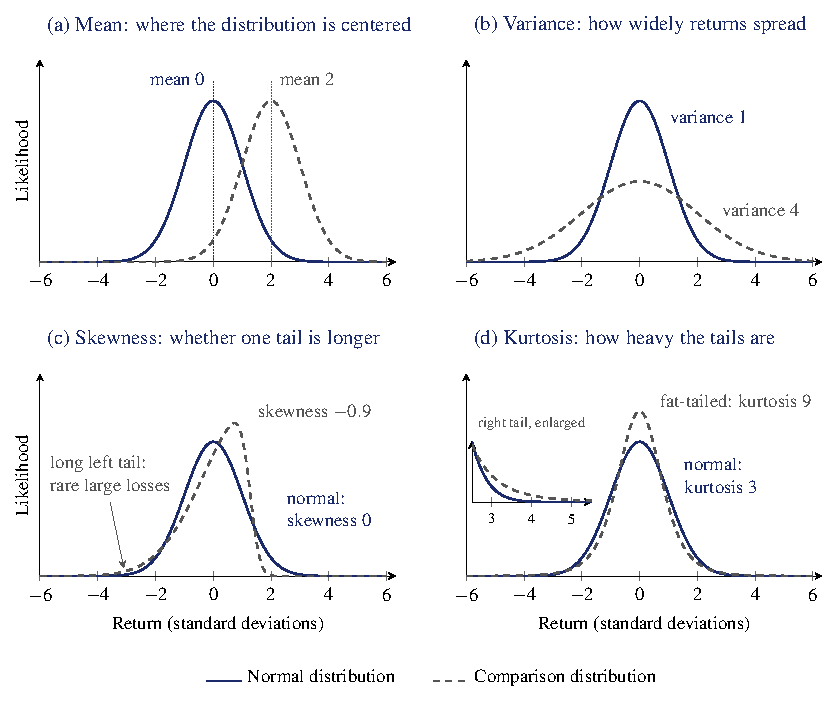
\includegraphics[width=0.7\linewidth]{images/fig03-0-moments.pdf}
\caption{The four moments of a distribution. Each panel compares the standard normal distribution (solid) with one that differs in a single respect. (a)~The mean sets the center. (b)~The variance sets the spread. (c)~Negative skewness lengthens the left tail, so large losses are more likely than large gains of the same size. (d)~Higher kurtosis puts more weight in the tails: the normal distribution has kurtosis 3, the fat-tailed one shown has kurtosis 9. Panels (c) and (d) keep the mean and variance of the normal distribution.}
\label{fig:03-moments}
\end{figure}

A fifth measure describes behavior over time. \textbf{Autocorrelation}\index{autocorrelation|textbf} is the correlation of a series with its own past values. The first-order autocorrelation ($\rho_1$) compares each month with the month before. A value near $+1$ means that a high month tends to be followed by another high month, a value near $-1$ means that it tends to be followed by a low month, and a value near zero means that the past says nothing about the next month. A return series with zero autocorrelation cannot be predicted from its own history.

\subsection{Linear regression and OLS assumptions}
\label{sec:03-regression}
A regression describes how a dependent variable, $y$, moves with an independent variable, $x$. Ordinary least squares\index{regression!ordinary least squares (OLS)} (OLS) fits
\begin{equation}
  y_t = \alpha + \beta x_t + \varepsilon_t
  \label{eq:03-ols}
\end{equation}
by choosing the intercept $\alpha$ and slope $\beta$ that minimize the sum of squared residuals $\sum \varepsilon_t^2$. The \textbf{residuals}\index{regression!residuals|textbf} $\varepsilon_t$ are the gaps between the actual values and the fitted line. The slope $\beta$ measures how much $y$ moves when $x$ moves by one unit, and the intercept $\alpha$ is the value of $y$ that the line predicts when $x$ is zero. The $R$-squared\index{regression!R-squared@$R^2$|textbf} ($R^2$) measures the share of the variance of $y$ explained by the regression, from 0 (none) to 1 (all).

A regression estimate also comes with a standard error, which measures how much the estimate would change if we drew a new sample. Section~\ref{sec:03-facts} examines when that standard error can be trusted. Until then, the chapter focuses on what the estimates themselves mean.

% =====================================================================
% PART ONE OF THE CHAPTER: THE DEVELOPMENT OF RISK DECOMPOSITION
% =====================================================================
\section{Risk and expected return}
\label{sec:03-decomposition}


The Capital Asset Pricing Model (CAPM) provides a fundamental framework for understanding the relationship between risk and expected return. According to the CAPM, investors are compensated for bearing systematic market risk, which cannot be eliminated through diversification. 

However, empirical evidence suggests that market risk alone cannot fully explain the differences in average returns across stocks. In particular, researchers have documented persistent return patterns associated with firm size, book-to-market equity, profitability, and investment behavior.

To address these empirical patterns, researchers developed a series of multifactor asset pricing models that extend the traditional CAPM. The central economic idea is that \textbf{firms differ in their exposure to various sources of systematic risk and in their economic characteristics.} These differences may help explain why some groups of stocks earn higher average returns than others.


\subsection{The CAPM: one source of priced risk}
\label{sec:03-capm}
The Capital Asset Pricing Model\index{capital asset pricing model (CAPM)} (Sharpe 1964, Lintner 1965, Mossin 1966) was the first formal risk decomposition, and it uses a single factor. It splits risk into two components. \textbf{Systematic risk}\index{risk!systematic|textbf} moves with the aggregate market and cannot be diversified away. \textbf{Idiosyncratic risk}\index{risk!idiosyncratic|textbf} is unique to individual assets and can be eliminated by holding a broad portfolio, a practice called \textbf{diversification}\index{diversification|textbf}. Because investors can remove idiosyncratic risk at almost no cost, the model says that they should not expect to be paid for bearing it. Only systematic risk earns a reward.

The CAPM says if every investor holds the market portfolio, then bad times are simply times when the market falls, and an asset's risk is measured by how much it falls along with the market. One number, the asset's sensitivity to the market, is then enough to set its expected return.


This one idea still underlies almost all of asset pricing, and its reach into practice is wide. Companies use the CAPM to set the discount rate\index{discount rate} for investment projects, and surveys find that most finance officers rely on it to estimate their cost of capital (Graham and Harvey 2001). The idea of alpha, the return beyond what market exposure explains, comes directly from the model, and its conclusion that the market portfolio is the best risky portfolio for every investor gave index funds their theoretical foundation.

Formally, the CAPM says that an asset's expected excess return\index{return!excess} is proportional to its \textbf{beta}\index{beta|textbf}, its sensitivity to the market:
\begin{equation}
  E[R^{e}_{i}] = \beta_i \, E[R^{e}_{m}], \qquad \beta_i = \frac{\operatorname{Cov}(R_i, R_m)}{\operatorname{Var}(R_m)}
  \label{eq:03-capm}
\end{equation}
Here $R_i$ is the asset's return, $R_m$ is the market's return and $R_f$ is the risk-free rate, so that $R^{e}_{i} = R_i - R_f$ and $R^{e}_{m} = R_m - R_f$ are their excess returns, as in Equation~\eqref{eq:excess-return}. The covariance $\operatorname{Cov}$ measures how two returns move together, and the variance $\operatorname{Var}$ measures how much one return moves on its own. A stock with a beta of 1.5 tends to rise 1.5\% when the market rises 1\%, so it carries one and a half times the market's systematic risk and should earn one and a half times the market's excess return.

The regression model is estimated in time series:
\begin{equation}
  R^{e}_{i,t} = \alpha_i + \beta_i R^{e}_{m,t} + \varepsilon_{i,t}
  \label{eq:03-capm-ts}
\end{equation}
This is Equation~\eqref{eq:03-ols} with the asset's excess return as $y$ and the market's excess return as $x$. The slope $\beta_i$ measures systematic market sensitivity. The intercept $\alpha_i$\index{alpha|textbf} (alpha) represents the average excess return that market exposure does not explain. The model predicts that $\alpha_i = 0$ for all assets, so a positive alpha is either evidence against the model or evidence of skill. Figure~\ref{fig:03-alpha} shows the two numbers on a scatter plot.

\begin{figure}[!htbp]
  \centering
  \begin{tikzpicture}[
    % Fitted regression: strategy = 1.16 + 1.15 * market
    declare function={fit(\x) = 1.16 + 1.15*\x;  zero(\x) = 1.15*\x;}
  ]
  \begin{axis}[
    scale only axis, width=0.41\linewidth, height=0.29\linewidth,
    axis lines=left,
    axis line style={-stealth, thin},
    xmin=-11, xmax=12.5, ymin=-12.5, ymax=16,
    xtick={-8,-4,0,4,8,12},
    ytick={-10,-5,0,5,10,15},
    tick label style={font=\footnotesize}, label style={font=\small},
    xlabel={Market excess return, $R^{e}_{m}$ (\% a month)},
    ylabel={Strategy excess return (\%)},
    clip=false,
  ]
    % Reference axes through zero
    \draw[gray!40] (axis cs:-11,0) -- (axis cs:12.5,0);
    \draw[gray!40] (axis cs:0,-12.5) -- (axis cs:0,16);

    % Monthly observations (illustrative)
    \addplot[only marks, mark=*, mark size=1.6pt, gray!60] coordinates {
      (0.51,2.80) (1.75,3.22) (-0.65,1.41) (-3.24,-0.57) (-1.41,-1.36)
      (-3.66,-2.80) (0.75,1.49) (6.13,8.66) (-1.57,-2.27) (-2.11,-2.05)
      (2.56,3.99) (2.00,4.86) (0.94,3.96) (-3.41,-4.63) (0.38,0.58)
      (3.42,6.19) (-5.15,-7.62) (-1.42,-1.08) (-7.49,-7.73) (-4.92,-2.80)
      (-7.24,-6.33) (-0.49,0.21) (-4.82,-4.97) (1.64,2.83) (1.16,4.75)
      (-0.29,0.31) (-10.07,-11.07) (-1.76,-0.34) (0.30,1.43) (0.98,2.12)
      (-5.93,-7.31) (-1.51,-0.55) (-3.61,-3.64) (-2.90,-0.54) (4.96,8.01)
      (-2.89,-2.20) (0.36,2.61) (4.21,5.75) (-1.95,0.41) (0.03,1.27)
      (0.96,3.20) (0.77,0.35) (-4.65,-3.75) (0.82,-0.15) (6.21,5.73)
      (-6.00,-6.26) (4.11,4.84) (1.00,2.66) (-2.19,1.80) (8.90,10.59)
      (3.70,4.74) (-4.54,-3.82) (0.81,2.90) (2.92,4.45) (-0.29,0.61)
    };

    % Zero-alpha line and fitted line
    \addplot[thick, dashed, fegray, domain=-11:12, samples=2] {zero(x)};
    \addplot[very thick, fenavy, domain=-11:12, samples=2] {fit(x)};
    \node[fenavy, anchor=west, font=\footnotesize] at (axis cs:12.3,{fit(12)+0.5}) {fitted line};
    \node[fegray, anchor=west, font=\footnotesize] at (axis cs:12.3,{fit(12)-3.5}) {zero-alpha line};

    % Slope triangle: run 3, rise 3 x beta
    \draw[fenavy] (axis cs:6,{fit(6)}) -- (axis cs:9,{fit(6)}) -- (axis cs:9,{fit(9)});
    \node[fenavy, anchor=north, font=\footnotesize] at (axis cs:7.5,{fit(6)-0.2}) {3};
    \node[fenavy, anchor=north west, font=\footnotesize, align=left] at (axis cs:9.3,{fit(6)-0.3})
      {rise $= 3\times$ beta\\beta $= 1.15$};

    % Alpha: the fitted line's value at a zero market return
    \fill[fenavy] (axis cs:0,1.16) circle (2.6pt);
    \draw[-stealth, fenavy] (axis cs:5.6,-3.4) -- (axis cs:0.4,0.9);
    \node[fenavy, anchor=north west, align=left, font=\footnotesize] at (axis cs:5.6,-2.6)
      {alpha $= 1.16$: the fitted line's\\value when the market return is 0};
  \end{axis}
  \end{tikzpicture}
\caption{Beta and alpha in a regression of a strategy's monthly excess returns on the market's. Beta is the slope of the fitted line; alpha is its height where the market's excess return is zero, the gap between the fitted line and a line with the same slope through the origin. Simulated data, with an alpha larger than any real strategy's so that it is visible.}
\label{fig:03-alpha}
\end{figure}

\textbf{The CAPM's variance decomposition.} Taking the variance of both sides of Equation~\eqref{eq:03-capm-ts} splits the asset's total risk into two parts. OLS makes the residuals uncorrelated with the market in the sample, so there is no cross term between them:
\begin{equation}
  \operatorname{Var}(R^{e}_{i}) = \beta_i^2 \operatorname{Var}(R^{e}_{m}) + \operatorname{Var}(\varepsilon_i)
  \label{eq:03-vardec-capm}
\end{equation}

Let's understand the two terms:
\begin{enumerate}
\item The first term is the \textbf{systematic variance}\index{variance!systematic|textbf}, the part that comes from exposure to the market, and 
\item the second is the \textbf{idiosyncratic variance}\index{variance!idiosyncratic|textbf}, the part that belongs to the asset alone. 
\end{enumerate}
The decomposition gives the regression's $R^2$ a direct economic meaning. The share of systematic variance in the total is exactly the $R^2$, so an $R^2$ of 0.9 says that 90\% of the asset's risk comes from the market and only 10\% is its own.

\begin{figure}[!htbp]
  \centering
  \begin{tikzpicture}[x=1cm, y=0.05cm]
    % Vertical axis: share of total variance, 0 to 100 percent
    \draw[-stealth, thin] (0,0) -- (0,108);
    \foreach \vdY in {0,50,100} {
      \draw (-0.08,\vdY) -- (0.08,\vdY);
      \node[anchor=east, font=\footnotesize] at (-0.1,\vdY) {\vdY};
    }
    \node[rotate=90, font=\small] at (-1.0,50) {Share of total variance (\%)};
    \draw[thin] (0,0) -- (6.6,0);

    % Bar 1: one stock, 31% systematic and 69% idiosyncratic
    \fill[fenavy!75] (0.8,0) rectangle (2.6,31);
    \fill[fenavy!15] (0.8,31) rectangle (2.6,100);
    \draw[fenavy] (0.8,0) rectangle (2.6,100);
    \node[white, font=\footnotesize, align=center] at (1.7,15.5) {systematic\\31\%};
    \node[fenavy, font=\footnotesize, align=center] at (1.7,65.5) {idiosyncratic\\69\%};
    \node[anchor=north, font=\small, align=center] at (1.7,-2) {One stock};

    % Bar 2: portfolio of 100 stocks, 98% systematic and 2% idiosyncratic
    \fill[fenavy!75] (3.8,0) rectangle (5.6,98);
    \fill[fenavy!15] (3.8,98) rectangle (5.6,100);
    \draw[fenavy] (3.8,0) rectangle (5.6,100);
    \node[white, font=\footnotesize, align=center] at (4.7,49) {systematic\\98\%};
    \draw[fenavy, thin] (5.6,99) -- (6.0,104);
    \node[fenavy, anchor=west, font=\footnotesize] at (6.0,104) {idiosyncratic 2\%};
    \node[anchor=north, font=\small, align=center] at (4.7,-2) {Portfolio of\\100 stocks};
  \end{tikzpicture}
  \caption{Splitting total variance into systematic and idiosyncratic parts with Equation~\eqref{eq:03-vardec-capm}. Each stock has a market beta of 1.2 and a residual standard deviation of 8\% a month, and the market's standard deviation is 4.5\% a month. Diversification leaves the systematic variance unchanged but divides the idiosyncratic variance by 100, so the systematic share, which equals the regression's $R^2$, rises from about 31\% to about 98\%. The numbers are illustrative.}
  \label{fig:03-vardec}
\end{figure}

The CAPM implies that a stock's expected return depends not on its total volatility, but on how sensitive it is to movements in the overall market. In practice, the CAPM provides a benchmark for determining the required return on investments, estimating the cost of equity capital for companies, evaluating portfolio performance, and making capital budgeting decisions. 

Empirical tests, however, show that the model fits the data less well than its influence suggests. If the CAPM were right, average returns would rise with beta along a straight line through the market portfolio, called the \textbf{security market line}\index{security market line|textbf}. Black, Jensen, and Scholes (1972) found that the security market line is flatter than predicted: low-beta stocks earn higher returns than the CAPM implies, while high-beta stocks earn lower returns (Figure~\ref{fig:03-sml}). 
The flatter security market line is important because it shows that the relationship between market risk and expected return is weaker than the CAPM predicts. In other words, low-beta stocks earn higher returns than the CAPM suggests, while high-beta stocks earn lower returns than expected. This means that taking on more market risk does not necessarily lead to proportionally higher returns. The finding challenges the CAPM's assumption that beta alone explains differences in expected returns and suggests that other factors may also influence stock performance. 

Later, Fama and French (1993) found that size and the book-to-market ratio\index{book-to-market ratio} explain differences in average returns that beta cannot. As a literal description of expected returns, the CAPM is therefore largely rejected, but it remains the benchmark against which every later model is built and tested. 
Interestingly, more research found that the stocks that the CAPM could not explain were not random. Their returns were related to certain company characteristics, such as size and book-to-market value. This suggested that factors beyond overall market risk also help explain why some stocks earn higher returns than others.




\begin{figure}[!htbp]
  \centering
  \begin{tikzpicture}[
    % CAPM security market line: E[R^e] = 8 * beta (% a year)
    % Illustrative empirical line, flatter: 3 + 3.5 * beta
    declare function={sml(\b) = 8*\b; emp(\b) = 3 + 3.5*\b;}
  ]
  \begin{axis}[
    scale only axis, width=0.43\linewidth, height=0.28\linewidth,
    axis lines=left,
    axis line style={-stealth, thin},
    xmin=0, xmax=1.95, ymin=0, ymax=15.5,
    xtick={0,0.5,1,1.5},
    ytick={0,4,8,12},
    xticklabel style={/pgf/number format/fixed},
    tick label style={font=\small}, label style={font=\small},
    xlabel={Beta, $\beta$},
    ylabel={Average excess return (\% a year)},
    clip=false,
  ]
    % CAPM prediction
    \addplot[fenavy, very thick, domain=0:1.85, samples=2] {sml(x)};
    \node[fenavy, anchor=west, font=\footnotesize] at (axis cs:1.86,{sml(1.85)}) {CAPM prediction};

    % Flatter line found in the data (illustrative)
    \addplot[fegray, thick, dashed, domain=0:1.85, samples=2] {emp(x)};
    \node[fegray, anchor=north west, font=\footnotesize] at (axis cs:1.86,{emp(1.85)+0.3}) {found in the data};

    % Ten beta-sorted portfolios (illustrative)
    \addplot[only marks, mark=*, mark size=1.8pt, fegray] coordinates {
      (0.55,5.1) (0.66,5.0) (0.76,5.9) (0.86,6.2) (0.95,6.1)
      (1.04,6.9) (1.14,6.7) (1.25,7.6) (1.37,7.5) (1.52,8.4)
    };

    % The market portfolio
    \fill[fenavy] (axis cs:1,8) circle (2.8pt);
    \node[fenavy, anchor=south east, font=\footnotesize] at (axis cs:0.97,8.2) {market};

    % Gap for high-beta stocks
    \draw[stealth-stealth, gray!70] (axis cs:1.6,{emp(1.6)}) -- (axis cs:1.6,{sml(1.6)});
    \node[anchor=west, font=\footnotesize, align=left] at (axis cs:1.63,11.8)
      {high-beta stocks earn\\less than predicted};
  \end{axis}
  \end{tikzpicture}
  \caption{The security market line. The CAPM predicts that average excess returns rise in a straight line with beta, passing through zero at a beta of zero and through the market's excess return at a beta of one (solid line). Tests that sort stocks into portfolios by beta typically find a flatter line with a positive intercept (dashed line and dots), so low-beta stocks earn more than predicted and high-beta stocks earn less (Black, Jensen and Scholes 1972). The numbers are illustrative.}
  \label{fig:03-sml}
\end{figure}

\subsection{The three-factor model: decomposing what the market leaves behind}
\label{sec:03-factors}
To capture the return variation that market beta misses, Fama and French (1993) introduced the three-factor model\index{Fama--French factors}. It adds two long--short portfolios to the market:
\begin{itemize}
  \item $SMB$\index{factor!SMB (size)} (Small Minus Big) is the return of small stocks minus the return of large stocks;
  \item $HML$\index{factor!HML (value)} (High Minus Low) is the return of value stocks, which have high book-to-market ratios, minus the return of growth stocks, which have low ones.
\end{itemize}
The model is
\begin{equation}
  R^{e}_{i,t} = \alpha_i + b_i R^{e}_{m,t} + s_i \,\mathrm{SMB}_t + h_i \,\mathrm{HML}_t + \varepsilon_{i,t}
  \label{eq:03-ff3}
\end{equation}
where $b_i$, $s_i$, and $h_i$ represent the asset's systematic exposures to the three factors, called its \textbf{factor loadings}\index{factor!loadings|textbf}. A portfolio of small value stocks, for example, would have a positive $s_i$ and a positive $h_i$, while a portfolio of large growth stocks would have negative values for both.

Each factor is a \textbf{long--short} portfolio. 
A long--short portfolio involves buying stocks in one group and short-selling stocks in another. Buying stocks means the investor owns them and hopes their prices will rise. Short-selling means borrowing stocks and selling them, hoping to buy them back later at a lower price. For example, the SMB factor buys stocks of small companies and short-sells stocks of large companies. The goal is to profit when small-company stocks perform better than large-company stocks.

The beauty of the Fama--French SMB factor is that it captures the difference in returns between small and large companies through a simple long--short strategy. By buying small-company stocks and short-selling large-company stocks, it isolates the performance of smaller firms relative to larger ones. This approach allows investors to measure the size effect directly, without relying on the overall direction of the stock market.

\textbf{The economic argument.} Why should size and value earn premia? 
Fama and French offered a risk-based explanation. They argued that small companies and financially distressed companies face risks that are not fully captured by the overall market factor. Small companies tend to share common return movements that differ from those of large companies. Similarly, value companies, which often have persistently weak earnings, tend to be more financially distressed than growth companies. Their stock returns reflect this additional source of risk. Investors may therefore require higher expected returns to hold these stocks. In this interpretation, SMB and HML capture risks beyond the overall market risk.

\textbf{Alpha decay.} Moving from the CAPM to three factors does not remove any return; it relabels it. Returns that the CAPM counted as alpha are reassigned to exposures to $SMB$ and $HML$. For the 25 portfolios sorted on size and book-to-market, the $R^2$ rises substantially, above 90\% for most portfolios, and the alphas shrink toward zero (Fama and French 1993). This \textbf{alpha decay}\index{alpha!decay|textbf} is the main practical consequence of the new decomposition: a manager who looked skilled under the CAPM may simply have held small value stocks.


\subsection{Beyond three factors: the Fama--French five-factor model}
\label{sec:03-multifactor}

The Fama--French three-factor model was later extended to include profitability and investment. These two additions were not entirely new
discoveries. They were motivated by earlier empirical studies showing that firms' profitability and investment decisions are related to
average stock returns. For example, Titman, Wei, and Xie (2004) found that firms with higher investment tend to earn lower subsequent
returns. Xing (2008) reported similar evidence. On the profitability side, Fama and French (2006) and Novy-Marx (2013) found that more
profitable firms tend to earn higher average returns. Building on this earlier research, Fama and French (2015) incorporated profitability
and investment into their existing three-factor model, creating the five-factor model.

The two new factors are \textbf{profitability} \index{factor!RMW (profitability)} ($RMW$, Robust Minus Weak) and
\textbf{investment}\index{factor!CMA (investment)} ($CMA$, Conservative Minus Aggressive). RMW measures the return difference between stocks of
highly profitable firms and those of less profitable firms. CMA measures the return difference between firms that invest conservatively
and those that invest aggressively. 

The five-factor model is:

\begin{equation}
  R^{e}_{i,t} = \alpha_i + b_i R^{e}_{m,t} + s_i \,\mathrm{SMB}_t + h_i \,\mathrm{HML}_t + r_i \,\mathrm{RMW}_t + c_i \,\mathrm{CMA}_t + \varepsilon_{i,t}
  \label{eq:03-ff5}
\end{equation}

Why should profitability and investment help explain stock returns? Fama and French (2015) state that a firm's value depends on its expected future cash flows and the return investors require.
Holding other things constant, firms with higher expected profitability should have higher expected returns. In contrast, firms that invest
more aggressively should have lower expected returns. 
Fama and French also found that, in their sample, the
HML factor added little explanatory power for average returns once profitability and investment were included. In other words, the
higher average returns of value stocks could largely be explained by their exposures to profitability and investment. This finding suggests
that the information captured by HML overlaps with that captured by RMW and CMA.

These extensions also change how we interpret alpha. Under the CAPM, alpha measures the return that cannot be explained by market risk.
Under the five-factor model, alpha measures the return that cannot be explained by market risk, size, value, profitability, and investment.
A different set of factors may produce a different alpha. Therefore, alpha is not simply a characteristic of an asset; it depends on the
asset pricing model used to evaluate it. Any discussion of alpha should make clear which model is being used.

\subsection{The factor zoo}
\label{sec:03-zoo}
The search did not stop at five or six factors. As Cochrane (2011) and Harvey, Liu, and Zhu (2016) document, intense backtesting has led to a ``zoo of factors''\index{factor zoo|textbf} comprising hundreds of published anomalies; Harvey, Liu, and Zhu counted more than 300. Each began life the same way as momentum and profitability did, as a pattern in average returns that the existing model could not explain.

Cochrane (2011) posed the question that the zoo raises: which characteristics really provide independent information about average returns, and which are the same few effects measured in different ways? The logic of risk decomposition offers one answer, and statistics offers another. The economic answer is that a factor deserves a place in the model only if there is a reason to expect its returns to track bad times, or a reason to expect a mispricing that arbitrage cannot remove. Without such a reason, adding factors becomes a mechanical exercise. Every new factor turns some alpha into beta, and with enough factors almost any alpha can be made to disappear, so the decomposition loses its power to tell skill from exposure.

The statistical answer is that a factor found by searching through hundreds of candidates must clear a higher bar than one proposed in advance. Most factors in the zoo were found by testing many candidate signals on the same few decades of U.S. data, which is exactly the kind of search that Chapter~\ref{ch:01} warned about. Section~\ref{sec:03-multiple} explains why such a search demands strict multiple-testing corrections. The zoo is where the two halves of this chapter meet: the risk decomposition supplies the candidate factors, and the $t$-statistic decides which of them survive.

Although researchers have proposed more than 300 factors, these
factors do not represent 300 completely different sources of risk.
Many are closely related to one another or are alternative ways of
measuring similar firm characteristics and return patterns. For
example, several factors capture different aspects of value,
profitability, investment, or momentum. Others are variations of
existing factors that use different accounting measures, portfolio
construction methods, or sample periods. The factors listed in
Table~\ref{tab:03-factor-zoo} represent some of the major ideas
behind this large body of research. Understanding these broad
categories makes the factor zoo easier to navigate.

\begin{table}[htbp]
\centering
\caption{Selected Factors in Empirical Asset Pricing}
\label{tab:03-factor-zoo}
\small
\begin{tabularx}{\textwidth}{l l X l}
\hline
\textbf{Factor} & \textbf{Name} & \textbf{Economic meaning} & \textbf{Key study} \\
\hline
MKT & Market
& Excess return of the overall stock market over the risk-free rate.
& Sharpe (1964) \\

SMB & Size
& Small firms tend to earn higher average returns than large firms.
& Fama and French (1993) \\

HML & Value
& High book-to-market firms tend to earn higher average returns than low book-to-market firms.
& Fama and French (1993) \\

MOM & Momentum
& Stocks that performed well recently tend to continue outperforming recent losers.
& Jegadeesh and Titman (1993) \\

RMW & Profitability
& Firms with strong profitability tend to earn higher average returns than firms with weak profitability.
& Fama and French (2015) \\

CMA & Investment
& Firms that invest conservatively tend to earn higher average returns than firms that invest aggressively.
& Fama and French (2015) \\

LIQ & Liquidity
& Stocks with greater exposure to liquidity risk may earn higher returns.
& Pástor and Stambaugh (2003) \\

ACC & Accruals
& Firms with high accruals tend to earn lower subsequent returns than firms with low accruals.
& Sloan (1996) \\

IVOL & Idiosyncratic volatility
& Stocks with high idiosyncratic volatility tend to earn lower subsequent returns than stocks with low volatility.
& Ang et al. (2006) \\

BAB & Betting Against Beta
& Low-beta stocks tend to outperform high-beta stocks on a risk-adjusted basis.
& Frazzini and Pedersen (2014) \\
\hline
\end{tabularx}
\end{table}


\subsection{Statistical significance versus economic significance}
\label{subsec:03-statistical-economic-significance}

When researchers identify a factor with a positive average return, an important question is whether the estimated premium is statistically significant. Statistical significance helps determine whether the observed premium is likely to reflect more than sampling variation. However, it does not tell us whether the premium is large enough to matter economically.

Consider a factor with an estimated average monthly return of 0.20\%. If its standard error is sufficiently small, the estimated premium may be statistically significant. Yet an annualized premium of approximately 2.4\% may or may not be attractive, depending on the risk involved and the costs of implementing the strategy. By contrast, a factor with a larger estimated premium may have substantial uncertainty and fail to meet conventional significance thresholds.

A common way to summarize a factor's historical performance is to calculate its annualized average return and Sharpe ratio. If $\bar{f}$ denotes the average monthly factor return and $s_f$ its monthly standard deviation, the annualized quantities are
\begin{equation}
  \text{Annualized premium}=12\bar{f},
  \qquad
  \text{Annualized Sharpe ratio}
  =\sqrt{12}\frac{\bar{f}}{s_f}.
  \label{eq:03-factor-sharpe}
\end{equation}
These calculations provide a convenient summary of the factor's historical return and risk. They rely on standard annualization conventions and should be interpreted with care, particularly when returns exhibit serial correlation.

Economic significance requires a broader assessment than the size of an estimated premium or its $t$-statistic. A strategy may generate a statistically significant return before costs but become unattractive after accounting for transaction costs, portfolio turnover, liquidity constraints and the practical difficulty of implementing the strategy. The results may also depend on the sample period, portfolio construction method and assumptions about trading.

There is another important distinction. A factor's historical premium does not, by itself, establish why the premium exists. Under a risk-based interpretation, investors earn compensation for bearing systematic risks. Under other interpretations, the premium may reflect mispricing, investor behavior or limitations in the empirical model. Establishing a reliable economic explanation requires more than observing a positive average return.

For these reasons, evaluating a factor requires several complementary questions:

\begin{itemize}
  \item \textbf{Statistical significance:} Is the estimated premium sufficiently precise to distinguish it from zero?
  \item \textbf{Economic significance:} Is the premium large enough to matter relative to the risk taken?
  \item \textbf{Implementability:} Does the premium remain attractive after transaction costs, turnover and liquidity constraints?
  \item \textbf{Economic interpretation:} Is there a convincing explanation for why the factor should earn a premium?
\end{itemize}

These questions are especially important in empirical asset pricing, where researchers may examine hundreds of candidate factors. A statistically significant result can arise by chance, particularly when many hypotheses are tested. Even a factor that survives statistical scrutiny must still demonstrate economic relevance and practical value. A credible factor discovery should therefore combine statistical evidence, economic reasoning and realistic investment considerations.



\subsection{Practical and institutional implications}
\label{sec:03-implications}

Multi-factor models have changed how investors evaluate fund
performance, manage portfolios, and make corporate investment
decisions. Three applications illustrate their importance.

\textbf{Asset management and identifying manager skill.}
A fund's excess return can be divided into two parts: returns
explained by exposure to common risk factors and the additional
return, called alpha, that the factors cannot explain. Investors
can now obtain exposure to many of these factors at relatively
low cost through index funds and factor-based funds. Therefore,
when evaluating an active fund manager, investors want to know
whether the manager's performance comes from genuine investment
skill or simply from holding stocks with certain factor
characteristics. Carhart (1997) found that momentum exposure and
fund expenses explain much of the apparent persistence in mutual
fund performance. Fama and French (2010) also found that very few
fund managers consistently generate returns that are high enough
to cover their costs.

\textbf{Performance evaluation and investment style.}
Multifactor models also help investors understand how a fund
generates its returns. By comparing a fund's returns with those
of different investment style indexes, researchers can identify
whether the fund follows a growth, value, or other investment
strategy, even without examining its individual holdings.
Sharpe (1992) demonstrated this approach using style analysis.
Institutional investors also monitor a manager's factor exposures
over time to detect changes in investment strategy, known as
\textbf{style drift}\index{style drift|textbf}. For example, if a
fund described as a value fund gradually loses its exposure to
the HML factor, its actual investment style may no longer match
its stated strategy.

\textbf{Corporate finance and the cost of capital.}
Companies also use asset pricing models to estimate the cost of
equity, which helps them decide whether a proposed project offers
a sufficient expected return. While the CAPM uses only market
risk, multifactor models allow companies to consider additional
sources of risk, such as firm size and other characteristics.
However, the CAPM remains the most widely used approach in
corporate practice (Graham and Harvey 2001). More factors do not
necessarily produce more accurate estimates. Fama and French
(1997) found that estimates of industry costs of equity were
highly uncertain under both the CAPM and the three-factor model,
with standard errors exceeding 3\% per year. Thus, multifactor
models may provide additional information for investment
decisions, but they do not eliminate the difficulty of estimating
the cost of capital accurately.


\subsection{The factor zoo and the multiple-testing problem}
\label{sec:03-multiple-testing}

The growing number of proposed risk factors raises an important
statistical question: how should we judge whether a newly discovered
factor is genuinely related to expected stock returns? Traditionally,
researchers often regard a $t$-statistic greater than approximately
2.0 as evidence of statistical significance at the 5\% level. This
convention is appropriate when testing a single hypothesis under the
usual statistical assumptions. However, asset pricing research
presents a different situation. Researchers have tested hundreds
of possible factors, often using overlapping data, similar
methodologies, and related measures of firm characteristics. When
so many hypotheses are tested, some will appear statistically
significant simply by chance.

Harvey, Liu, and Zhu (2016)
address this problem. They argue that the traditional significance
threshold is too low for a field in which researchers have tested
so many potential explanations for the cross-section of stock
returns. Their central message is that statistical significance
must be evaluated in light of the entire search process, not just
the final result reported in an individual paper.

\textbf{Why testing many factors creates a problem.}
To understand their argument, consider a simple example. Suppose
a researcher tests 100 factors, none of which has a genuine
relationship with expected returns. 

If each factor is tested
individually at the 5\% significance level, Assuming
the tests are independent, the probability of obtaining at least
one false positive is
\begin{equation}
  1-(1-0.05)^{100} \approx 99.4\%. \nonumber
\end{equation}

The probability of avoiding a false positive is 1-0.05 = 0.95. 
$0.95^{100}$ represents the probability that all 100 tests avoid false positives. 
Subtracting this probability from 1 gives \textbf{the probability of at least one false positive}, which is approximately 99.4\%.

In other words, when 100 independent factors, each with a true premium of zero, are tested at the 5\% significance level, 
there is approximately a 99.4\% 
chance that at least one will incorrectly appear to have a significant premium.

This issue is known as the \textbf{multiple-testing problem}.
\index{multiple-testing problem|textbf} A conventional $t$-test
evaluates one hypothesis at a time. It does not account for the
number of other hypotheses that researchers have examined.
Consequently, a factor with a $t$-statistic of 2.1 may appear
significant when considered in isolation, even though the result
is much less convincing after accounting for the many other
factors that researchers have tried.

There is another difficulty: researchers and academic journals
are more likely to report statistically significant findings than
unsuccessful experiments. A factor that produces a $t$-statistic
of 2.5 may be published, while another factor that produces a
$t$-statistic of 0.8 may never appear in a journal article. The
published literature therefore contains a disproportionate
number of successful results. This phenomenon is known as
\textbf{publication bias}\index{publication bias|textbf}. It
creates a form of selection bias: the factors we observe are
already those that have passed an initial significance threshold.

Harvey, Liu, and Zhu emphasize that the number of published
factors is not the same as the total number of factors researchers
have tested. The unsuccessful experiments that never become
publicly available are also part of the research process and
should be considered when evaluating the reliability of reported
discoveries.

\textbf{How many factors have researchers actually tested?}
To investigate the scale of the problem, Harvey, Liu, and Zhu
(2016) assembled a database of 313 research papers that proposed
and tested 316 factors related to the cross-section of expected
stock returns. 

The list of 316 factors illustrates the extensive search for
variables that can explain differences in average stock returns.
The 316 factors do
not necessarily represent 316 independent sources of risk.
But more importantly, the authors recognized that factors that failed to
produce significant results were unlikely to be published.
Their statistical framework therefore attempts to account for
these unobserved tests rather than treating the published
literature as the complete record of research activity.

The authors then evaluate how demanding the statistical
significance threshold should be when researchers test many
potential factors. They consider several approaches that
differ in how strictly they control the possibility of false
discoveries. 


After accounting for multiple testing, unpublished
experiments and correlations among factors, they find
that the required $t$-statistic varies with the statistical
method and assumptions. Some stricter approaches require
a value more than 3.92. Their widely cited recommendation,
however, is that a newly discovered factor should generally
have a $t$-statistic greater than 3.0.
The precise threshold is not a universal constant. It depends
on the number of tests, the dependence among test statistics,
the assumed number of unreported experiments, and the chosen
error-control procedure. 

\subsection{Economic magnitude}
A statistically significant result is also not the same
as an economically important result. A factor may have a
high $t$-statistic but a very small average return, making
its practical investment value limited. Conversely, a
factor with an economically meaningful estimated premium
may not be statistically precise. Statistical significance,
economic magnitude, and a sound economic explanation
should therefore be considered together.

Finally, multiple-testing adjustments do not replace
careful empirical methods. Harvey, Liu, and Zhu take the
reported $t$-statistics as given and assume that the
underlying studies have appropriately addressed issues
such as heteroskedasticity, autocorrelation, and data
errors. 

\section{Lab~\thechapter: Replicating multifactor models and investigating the factor zoo}
\label{sec:03-lab}

\begin{callout}
\textbf{Lab~\ref{ch:03} at a glance.} \emph{Claim on trial:} additional factors improve our ability to explain differences in portfolio returns, but testing many candidate factors can produce false discoveries. \emph{Data:} monthly returns on the 25 Fama--French portfolios formed on size and book-to-market, together with the market, size and value factors, from the Kenneth R. French Data Library\index{Kenneth French data library}. \emph{Tools:} Python with pandas, NumPy, SciPy and matplotlib, plus the fintest module. \emph{Time:} about two hours, including the guided notebook. \emph{Code:} repository folder \texttt{ch03-multifactor-models/}.
\end{callout}

This lab examines two important questions in empirical asset pricing. First, do additional risk factors improve our ability to explain stock returns? Second, when researchers test hundreds of potential factors, how can we distinguish genuine discoveries from results that arise by chance?

Part~A replicates the central empirical analysis of Fama and French (1993), using the 25 portfolios formed on size and book-to-market to estimate the CAPM and the Fama--French three-factor model. Readers compare the explanatory power and estimated factor exposures of the two models. Part~B conducts a controlled multiple-testing experiment inspired by Harvey, Liu and Zhu (2016), demonstrating why conventional significance thresholds can produce many false discoveries when researchers examine a large number of candidate factors. Part~C examines the economic significance of factor premiums and considers whether statistically significant results translate into attractive investment opportunities.

\subsection*{Part A: Replicating the Fama--French three-factor model}

The 25 portfolios formed on size and book-to-market are the classic \textbf{test assets}\index{factor!test assets|textbf} of Fama and French (1993): the portfolios whose returns an asset-pricing model is designed to explain. The lab uses monthly data beginning in July 1963 and estimates two models for each portfolio.

The first is the CAPM:
\begin{equation}
  R^{e}_{i,t}
  = \alpha_i+\beta_{i,M}R^{e}_{m,t}+\varepsilon_{i,t}.
  \label{eq:03-lab-capm}
\end{equation}

The second is the Fama--French three-factor model:
\begin{equation}
  R^{e}_{i,t}
  = \alpha_i+\beta_{i,M}R^{e}_{m,t}
  +\beta_{i,S}SMB_t
  +\beta_{i,H}HML_t+\varepsilon_{i,t},
  \label{eq:03-lab-ff3}
\end{equation}
where $R^{e}_{m,t}$ is the market excess return, which the French library labels Mkt-RF, $SMB$ is the return on small stocks minus large stocks, and $HML$ is the return on high book-to-market stocks minus low book-to-market stocks.

For each portfolio, the lab reports the estimated alpha, factor loadings and $R^2$. Readers then compare the results from the two models. Adding $SMB$ and $HML$ should improve the model's ability to explain the returns of portfolios formed on size and book-to-market. The estimated factor loadings also reveal how different portfolios are exposed to market, size and value risks.

The results illustrate an important distinction. A higher $R^2$ means that the model explains more of the variation in portfolio returns. It does not necessarily mean that the model fully explains differences in average returns or that every estimated alpha is zero. The estimated alphas provide an additional way to examine the returns that remain unexplained by the included factors.

\subsection*{Part B: A multiple-testing experiment}

The factor zoo creates a different statistical problem. If researchers test enough candidate factors, some will appear significant simply by chance, even when none has a genuine return premium.

To see why, consider 1,000 candidate factors, each of which has a true expected premium of zero. The lab simulates monthly returns for these factors and tests whether the average premium of each factor differs from zero. Because the true premium is known to be zero, every rejection is a false discovery.

The experiment applies two significance thresholds:
\begin{itemize}
  \item The conventional threshold, $|t|>1.96$, corresponding approximately to a two-sided 5\% test.
  \item A more demanding threshold, $|t|>3.0$, inspired by the recommendations of Harvey, Liu and Zhu (2016).
\end{itemize}

The lab repeats the experiment and records the number of false discoveries under each threshold. With 1,000 independent tests and a conventional 5\% significance level, we would expect approximately 50 false positives on average, even though none of the factors has a genuine premium. A higher threshold substantially reduces this number.

This experiment illustrates the basic logic behind the multiple-testing problem. The more candidate factors researchers examine, the greater the chance that some will appear significant by coincidence. Harvey, Liu and Zhu (2016) argue that the conventional $t$-statistic threshold of approximately 2 is too weak for many new factor discoveries and that a higher hurdle is needed.

The simulation is deliberately simplified: it treats the candidate factors as independent and assumes that their true premiums are zero. In actual asset-pricing research, candidate factors may be correlated, and some may have genuine economic foundations. The experiment is therefore not a replication of Harvey, Liu and Zhu (2016), but a demonstration of the statistical problem that motivates their analysis.

\subsection*{Part C: Statistical and economic significance}

A factor can have a statistically significant premium without offering an attractive investment opportunity. The final part of the lab examines the size of the estimated factor premiums and their potential economic value.

For each factor, the lab calculates its average monthly return, annualized premium and annualized Sharpe ratio. For a factor with monthly mean return $\bar{f}$ and standard deviation $s_f$, the annualized quantities are
\begin{equation}
  \text{Annualized premium}=12\bar{f},
  \qquad
  \text{Annualized Sharpe ratio}
  =\sqrt{12}\frac{\bar{f}}{s_f}.
  \label{eq:03-lab-sharpe}
\end{equation}

Readers then consider whether the estimated premiums are large enough to matter in practice. A strategy may have a statistically significant premium but require frequent trading, substantial turnover or investment in illiquid stocks. Transaction costs and implementation constraints can reduce or eliminate its apparent advantage.

The purpose is not to decide whether every factor is investable. Rather, it is to recognize that statistical evidence is only one part of evaluating an investment strategy. A credible finding should also have an economically meaningful magnitude and remain attractive after realistic implementation costs are considered.

\emph{[Draft note: the regression results and factor-premium estimates are generated from the Kenneth R. French Data Library at the time of publication. The multiple-testing experiment uses simulated data with known zero premiums. The book prints the numerical results; the accompanying notebook allows readers to reproduce the analysis.]}

\section{Verdict}
\label{sec:03-verdict}

Readers judge the claim by comparing the results from all three parts. The expected verdict is \textbf{survives, with conditions}. The Fama--French three-factor model should explain more of the variation in the 25 size-and-book-to-market portfolios than the CAPM. Its additional factors capture systematic differences in portfolio returns that the market factor alone does not explain. However, a higher $R^2$ does not guarantee that all pricing errors disappear or that the model fully explains differences in expected returns.

The multiple-testing experiment reveals a separate limitation. When researchers examine hundreds of candidate factors, conventional significance thresholds can produce many false discoveries. A more demanding statistical hurdle helps, but it does not replace economic reasoning, theoretical motivation or out-of-sample validation.

Finally, statistical significance does not guarantee economic value. Factor premiums must be large enough to matter after considering risk, transaction costs and implementation constraints. The broader lesson is that a convincing factor discovery requires more than a significant $t$-statistic: it should help explain return differences, withstand appropriate statistical scrutiny and make economic sense.

\section{What investors can use}
\label{sec:03-investors}

Most investors will never compute a Newey--West standard error or a GRS statistic, but the ideas in this chapter translate directly into questions about any statistical claim.

\textbf{Rules of Thumb:}
\begin{enumerate}
  \item \textbf{Unbundle alpha from factor beta.} Do not pay active fees for static loadings on known factors ($SMB$, $HML$, $UMD$), because those exposures can be bought cheaply through index and factor funds.
  \item \textbf{Count independent observations.} $T$ monthly observations with a $k$-month horizon provide only about $T/k$ independent periods. Fifty years of five-year returns is ten independent observations, not six hundred.
  \item \textbf{Demand higher cutoffs.} Require $t > 3.0$ for proposed factor anomalies to adjust for search bias, and remember that across 25 portfolios one or two will look significant by chance.
  \item \textbf{Convert $t$-statistics to net returns.} Evaluate alpha after transaction costs, short-selling fees, and turnover. A significant alpha smaller than the fund's fee is worth nothing to the investor.
\end{enumerate}

\textbf{Questions to Ask Fund Managers:}
\begin{itemize}
  \item What standard errors were used, and do your results hold under Newey--West HAC and block bootstrap methods?
  \item What fraction of net performance comes from true alpha versus systematic factor exposures?
  \item How many candidate models or variations were backtested before selecting this strategy?
  \item If you forecast over long horizons, how many non-overlapping periods does your sample contain?
  \item What is the confidence interval for your alpha, and how large is it after fees and trading costs?
\end{itemize}

\section*{Exercises}

\subsection*{Conceptual (all readers)}
\begin{enumerate}
  \item An active equity manager reports a CAPM alpha of 3.2\% per year ($t = 2.5$). Under a Fama--French three-factor model, the alpha drops to 0.1\% ($t = 0.2$), with an $SMB$ loading of 0.70 and an $HML$ loading of 0.50. Explain the source of the manager's excess return, and what it implies for the fee the manager should charge.
  \item A stock has a market beta of 0.8, a residual standard deviation of 6\% a month, and the market's standard deviation is 4.5\% a month. Use Equation~\eqref{eq:03-vardec-capm} to compute the share of its variance that is systematic. What would the share be for an equally weighted portfolio of 50 such stocks with independent residuals?
  \item Fama and French (2015) found that the value factor becomes redundant once profitability and investment factors are added. Using the dividend discount model argument of Section~\ref{sec:03-multifactor}, explain why value stocks might load on these two factors, and discuss what the finding implies for reading $HML$ as a distress factor.
  \item Explain why adding factors to a model can always make an alpha smaller, and state what economic and statistical evidence you would require before accepting a newly proposed factor.
  \item Daily returns show minimal autocorrelation, yet absolute daily returns show strong autocorrelation. Explain how both statements can be true, and why this matters for standard errors.
  \item A long-horizon regression of 5-year returns on dividend yields uses 50 years of monthly data ($T=600$, $k=60$). How many independent observations does it contain, and why are classical $t$-statistics misleading?
  \item Why must a time-series bootstrap resample blocks of observations rather than individual months?
  \item Explain why a factor alpha with $t = 3.2$ might lack economic significance, and list what you would need to know before investing in it.
\end{enumerate}

\subsection*{Lab extensions (technical readers)}
\begin{enumerate}
  \setcounter{enumi}{8}
  \item Replicate Part B of Lab~\ref{ch:03} across two sub-samples: 1963--1992 and 1993--present. Compare changes in factor risk premia and GRS test rejections.
  \item Compute $t$-statistics for 25 portfolio alphas using four methods: Classical OLS, White, Newey--West, and Stationary Block Bootstrap. Identify portfolios with the largest SE discrepancies, and explain what features of their returns might cause them.
  \item Pair monthly returns with 1,000 simulated non-predictive predictors ($\rho = 0.98$). Run long-horizon regressions ($k=1$ to $60$) and plot false-positive rates for OLS, Newey--West, and Hodrick standard errors. Then set the correlation between predictor shocks and return shocks to $-0.9$ and describe how the Stambaugh bias changes the results.
\end{enumerate}

  
% Chapter 4 -- Claim: A Profitable Backtest Means a Profitable Strategy
% Requires: amsmath, amssymb, booktabs, array, tabularx, graphicx, tcolorbox (breakable, skins), hyperref or url.
% Defines the callout box only if the preamble has not.
\providecolor{fenavy}{HTML}{1B2A6B}
\providecolor{feshade}{HTML}{F3F5FA}
\providecolor{feorange}{HTML}{B8481C}
\makeatletter
\@ifundefined{callout}{%
  \newtcolorbox{callout}{breakable, enhanced,
    colback=white, colframe=gray!70, boxrule=0.5pt, arc=1mm,
    borderline west={2.5pt}{0pt}{gray!70},
    left=8pt, right=8pt, top=4pt, bottom=4pt}%
}{}
\makeatother

\chapter{Claim: A Profitable Backtest Means a Profitable Strategy}
\label{ch:04}

Chapter~\ref{ch:03} described the factor zoo: hundreds of published patterns in average returns that the CAPM cannot explain. Almost all of them were documented with \textbf{paper returns}\index{return!paper versus implementable}, the returns of portfolios that are rebuilt every month at recorded closing prices, in any size, at no cost. Researchers have long known that this is a simplification, and the reason it matters goes back to the definition of an efficient market. Jensen (1978) argued that a market is efficient with respect to some information if no one can earn \emph{economic} profits by trading on it, which means profits after all the costs of trading. Grossman and Stiglitz (1980) went further. They showed that prices cannot reflect all information perfectly, because then no one would be paid for the cost of gathering it. On this view, some return patterns should survive on paper but not after costs, since costs are exactly what keeps them from being traded away.

The question became pressing in the early 2000s, when researchers began to price the trades behind the best-known anomalies\index{anomaly}. Lesmond, Schill and Zhou (2004) found that momentum\index{momentum} trades concentrate in stocks that are expensive to trade, and concluded that its profits largely disappear after costs. Korajczyk and Sadka (2004) measured how prices move when large orders are executed. They found that momentum profits shrink as the size of the portfolio grows, and that even versions designed to trade cheaply could absorb only about \$5 billion, at December 1999 market values, before the profits vanished. Novy-Marx and Velikov (2016) then estimated trading costs for 23 well-known anomalies and found that most strategies that trade more than half of their portfolio each month lose their significance after costs. Frazzini, Israel and Moskowitz (2018) challenged the size of these estimates. Using a large manager's own trading records, they found costs far below what the academic estimates assumed. The same patterns therefore look profitable or unprofitable depending on whose costs are used.

The answer matters for both research and practice. For research, it decides whether an anomaly is evidence against market efficiency or only a pattern that no investor could exploit. For practice, it decides which published strategies are worth running, how much money each can manage, and whether a fund that offers them can deliver its backtest. The claim on trial\index{claims-on-trial method} is the assumption behind most published backtests\index{backtest}: \textbf{a strategy that is profitable in a backtest is profitable to trade.}

The chapter draws on two papers about the cost of trading. Novy-Marx and Velikov (2016) estimate how much of each published anomaly survives trading costs. Frazzini, Israel and Moskowitz (2018) use real institutional trades to show that costs can be lower than academic estimates, but that they grow with the size of the fund. The lab in Section~\ref{sec:04-lab} replicates the main calculations of both papers in order to find out which strategies stay profitable after costs, what cost level would wipe out each one, and how much money each can manage.

By the end of the chapter you will be able to:

\begin{itemize}
  \item read a limit order book\index{order book}, and explain bid--ask spreads\index{bid--ask spread}, market orders\index{market order} and limit orders\index{limit order};
  \item explain how long and short positions work, what short selling\index{short selling} costs, and what a zero-investment portfolio\index{long--short portfolio} is;
  \item break trading costs into commissions, bid--ask spreads, market impact\index{market impact} and the costs of short selling, and estimate the main ones from public data;
  \item compute a strategy's turnover\index{turnover} and explain what drives it;
  \item convert gross returns into net returns, and compute the break-even cost\index{transaction costs!break-even} a strategy can bear;
  \item estimate how market impact limits the money a strategy can manage;
  \item design strategies that trade less without giving up much of their signal.
\end{itemize}

In the lab you will take three of the best-known long--short strategies, value, momentum and short-term reversal\index{short-term reversal}, measure how much each trades, charge each for trading, and see how their ranking changes. A simulated market with known expected returns\index{return!expected} then shows how much a cost-aware design can recover.

\section{Foundations: how stocks are traded and sold short}
\label{sec:04-foundations}

\subsection{The order book}

Most stocks trade on electronic exchanges. Each exchange keeps a \textbf{limit order book}\index{order book|textbf}, which is a list of standing offers to buy and to sell. The offers to buy are called \textbf{bids}, and the offers to sell are called \textbf{asks}. Each offer states a price and a number of shares (Figure~\ref{fig:04-book}).

The highest bid and the lowest ask are the \textbf{best quotes}. The gap between them is the \textbf{bid--ask spread}\index{bid--ask spread|textbf}, and the price halfway between them is the \textbf{midpoint}\index{midpoint|textbf}. Spreads are usually quoted in \textbf{basis points}\index{basis point|textbf} of the midpoint. A basis point is a hundredth of a percent, so 100 basis points make 1\%.

\begin{figure}[htbp]
  \centering
  \scalebox{0.8}{%
\begin{tikzpicture}[
    x=0.014cm, y=0.5cm,     % x: shares; y: price levels
    ask/.style={fill=feorange!35},
    bid/.style={fill=fenavy!75},
    price/.style={anchor=east, font=\small},
  ]
    % Asks (sellers) above the midpoint: level / price / shares
    \foreach \wfL/\wfP/\wfQ in {1/50.02/200, 2/50.03/350, 3/50.04/300,
                                4/50.05/450, 5/50.06/500} {
      \fill[ask] (0,\wfL+0.5-0.38) rectangle (\wfQ,\wfL+0.5+0.38);
      \node[price] at (-10,\wfL+0.5) {\$\wfP};
    }
    % Bids (buyers) below the midpoint
    \foreach \wfL/\wfP/\wfQ in {1/49.98/250, 2/49.97/300, 3/49.96/400,
                                4/49.95/350, 5/49.94/550} {
      \fill[bid] (0,-\wfL-0.5-0.38) rectangle (\wfQ,-\wfL-0.5+0.38);
      \node[price] at (-10,-\wfL-0.5) {\$\wfP};
    }

    % Best ask and best bid
    \draw[feorange, thick] (0,1.12) rectangle (200,1.88);
    \draw[fenavy, thick]   (0,-1.88) rectangle (250,-1.12);
    \node[feorange, anchor=west, font=\small] at (215,1.5)
      {best ask: buyers pay \$50.02};
    \node[fenavy, anchor=west, font=\small] at (265,-1.5)
      {best bid: sellers get \$49.98};

    % Midpoint
    \draw[densely dashed] (-10,0) -- (560,0);
    \node[anchor=south east, font=\small, inner sep=2pt] at (560,0) {midpoint \$50.00};

    % Spread bracket
    \draw[decorate, decoration={brace, amplitude=4pt}]
      (-150,-1.5) -- (-150,1.5)
      node[midway, anchor=east, xshift=-5pt, align=right, font=\small]
      {spread\\\$0.04\\(8 bp)};

    % Headings and size axis
    \draw[thin] (0,-6.1) -- (0,6.1);
    \node[feorange, font=\small\bfseries, anchor=south west] at (0,6.1)
      {Asks: sellers' limit orders};
    \draw[-stealth, thin] (0,-6.1) -- (580,-6.1)
      node[anchor=west, font=\small] {shares};
    \node[fenavy, font=\small\bfseries, anchor=north west] at (0,-6.3)
      {Bids: buyers' limit orders};
  \end{tikzpicture}%
}
  \caption{A limit order book. Sellers' asks sit above the midpoint and buyers'
    bids below it. A buyer who wants to trade at once pays the best ask,
    \$50.02; a seller receives the best bid, \$49.98. The gap of \$0.04,
    8 basis points of the \$50.00 midpoint, is the bid--ask spread.}
  \label{fig:04-book}
\end{figure}

\textbf{Worked example.} In Figure~\ref{fig:04-book}, the best bid is \$49.98 and the best ask is \$50.02. The midpoint is \$50.00 and the spread is \$0.04, which is $0.04/50 = 0.0008$, or 8 basis points. An investor who buys at the ask and sells again at once at the bid loses those 8 basis points. The cost of one side of the trade, called the \textbf{one-way cost}\index{transaction costs!one-way and round-trip}, is half the spread: 4 basis points.

\subsection{Market and limit orders}

There are two basic ways to trade.

\begin{itemize}
  \item A \textbf{market order}\index{market order|textbf} trades at once against the best available quote. A buyer pays the ask and a seller receives the bid. A market order \emph{takes} liquidity\index{liquidity}, and it pays the spread for doing so.
  \item A \textbf{limit order}\index{limit order|textbf} names a price and waits in the book until someone trades against it. A limit order \emph{supplies} liquidity and may earn the spread. Its risk is that it may never be filled, or that it is filled just before the price moves against it.
\end{itemize}

Large orders are usually split into many small ones and executed over hours or days, so that each piece moves the price less.

\subsection{Who provides liquidity}

\textbf{Market makers}\index{market maker|textbf} and high-frequency traders post bids and asks all day and earn the spread. In return they bear two risks. The first is \textbf{inventory risk}: prices may move while they hold shares they have bought but not yet sold. The second is the risk of trading with investors who know more than they do. Both risks are larger for small, volatile and thinly traded stocks, which is why spreads are wider for those stocks.

\subsection{Long and short positions}

A \textbf{long} position owns a security and gains when its price rises. A \textbf{short} position borrows shares, sells them, and later buys them back to return them. It gains when the price falls.

Short selling has costs that a long position does not. The short seller must pay any dividends to the lender. The short seller must also post \textbf{collateral}\index{collateral|textbf}, cash or securities held as security for the loan, and pay a \textbf{borrowing fee}\index{borrowing fee|textbf} set in the securities-lending market. Most large stocks are cheap to borrow. A minority are hard to borrow and expensive, and the lender can \textbf{recall} the loan at any time, which forces the short seller to buy the shares back.

\subsection{Long--short portfolios}

Academic factors such as HML\index{factor!HML (value)}, introduced in Section~\ref{sec:03-factors}, are \textbf{zero-investment} portfolios. They hold one dollar long and one dollar short, so the money raised by the short sale pays for the long side. A factor's ``return'' is therefore the difference between the returns of the two sides. It is a spread, not a return on money invested. A real long--short fund must hold capital against both sides, and it quotes its returns relative to that capital.

\section{Paper returns versus implementable returns}
\label{sec:04-paper}

The factor returns in the Kenneth French Data Library\index{Kenneth French data library}, like most portfolio returns in academic research, are \textbf{paper returns}\index{return!paper versus implementable|textbf}. Each month the portfolio is rebuilt from the latest sorts, at closing prices, with no charge for trading. This construction is simple and transparent, which is why the data are so useful. But it answers the question ``what pattern exists in returns?'' It does not answer the question ``what could an investor have earned?''

An \textbf{implementable return} is one that an investor could actually have earned. It differs from a paper return in four ways.

\begin{enumerate}
  \item \textbf{Trading costs.}\index{transaction costs|textbf} Every purchase pays more than the midpoint, and every sale receives less. Large orders also move the price.
  \item \textbf{Short-selling costs and limits.} Selling short requires borrowing shares. Borrowing costs a fee, may be impossible for some stocks, and can be recalled.
  \item \textbf{Timing and execution.} A signal computed from closing prices cannot be traded at those same prices. Orders take time to fill, and fast-moving signals lose value while they wait.
  \item \textbf{Scale.} A strategy that works with \$10 million may not work with \$10 billion, because the trades themselves change prices.
\end{enumerate}

None of these makes a paper return wrong. A pattern that cannot be traded profitably may still tell us something about risk or about how prices are formed. But a claim about profits needs an implementable return, and the two can differ by more than the whole premium.

The gap is largest for strategies that trade often, that hold small or illiquid stocks, or that rely on the short side. It is smallest for slow strategies in large stocks. This is one reason the market portfolio is so hard to beat after costs: it hardly trades at all.

\section{The anatomy of trading costs}
\label{sec:04-anatomy}

The cost of a trade has several parts, and each behaves differently.

\begin{center}
\small
\begin{tabularx}{0.9\linewidth}{@{}>{\raggedright\arraybackslash}p{0.19\linewidth}>{\raggedright\arraybackslash}X>{\raggedright\arraybackslash}p{0.32\linewidth}@{}}
\toprule
Component & What it is & How it scales \\
\midrule
Commissions and fees & Payments to brokers and exchanges & Small for institutions today; roughly proportional to the amount traded \\
Bid--ask spread & Buying at the ask and selling at the bid, above and below the midpoint & Proportional to the amount traded; wider for small, volatile and illiquid stocks \\
Market impact & The price moving against an order while it is executed, because the order carries information or demands liquidity & Grows faster than the trade, roughly with the square root of the order's size relative to volume \\
Delay and opportunity cost & Prices moving before the order is filled, or trades not made at all & Largest for fast signals \\
Short-selling costs & Fees to borrow shares, the risk of recall, and rules that restrict shorting & Small for most stocks, very large for a few \\
\bottomrule
\end{tabularx}
\end{center}

The unit used throughout this chapter is the \textbf{one-way cost}\index{transaction costs!one-way and round-trip|textbf}: the cost of buying, or of selling, one dollar of stock, as a fraction of that dollar. For a small trade it is roughly half the bid--ask spread plus commissions. A \textbf{round trip}, buying and later selling, costs twice the one-way cost.

\textbf{Costs have fallen, but unevenly.} In 2001 U.S. stock prices moved from fractions of a dollar to decimals, a change called \textbf{decimalization}\index{decimalization|textbf}. Spreads narrowed sharply after it, and narrowed further as electronic trading spread. Large stocks now trade at spreads of a few basis points, while small, illiquid stocks still cost far more. This matters when we read long histories. A strategy tested from 1963 faced costs in its early decades that were several times today's. Applying today's costs to the whole history flatters the past, and applying the past's costs to today understates what is possible now.

\textbf{Short selling.}\index{short selling|textbf} D'Avolio (2002) studied the market for borrowing stock. He found that the large majority of U.S. stocks were cheap to borrow, but that a small set of ``special'' stocks carried high fees, and that these were often the stocks that short sellers most wanted to sell. Loans can also be recalled at inconvenient times, and regulators can ban short selling outright, as the U.S. Securities and Exchange Commission did for financial stocks in September 2008.

These limits matter for prices as well as for costs. Miller (1977) argued that when pessimists cannot sell short, prices reflect only the views of optimists, so overpricing can last. Stambaugh, Yu and Yuan (2012) found that anomaly returns come more from the short side than from the long side, especially after periods of high investor sentiment, which is where short-sale limits matter most. A long--short paper portfolio that ignores these frictions can overstate what is achievable by much of its premium.

The lab uses a single one-way cost and a single borrowing fee, so that the calculations are easy to follow. Real costs vary across stocks and over time, and Section~\ref{sec:04-measuring} shows how they can be estimated.

\section{Measuring costs from public data}
\label{sec:04-measuring}

The best measure of trading costs is a trader's own record. Perold (1988) proposed the \textbf{implementation shortfall}\index{implementation shortfall|textbf}, which compares the value of a paper portfolio, priced when the decision was made, with the value of the portfolio actually achieved. It captures spreads, impact, delay and trades that were never completed. Most researchers do not have such records, so the field relies on estimates.

\textbf{From quotes and trades.} With intraday data, such as the TAQ (Trade and Quote) database of every U.S. trade and quote, two spreads can be measured.

\begin{itemize}
  \item The \textbf{quoted spread}\index{bid--ask spread!quoted|textbf} is the gap between the best bid and the best ask.
  \item The \textbf{effective spread}\index{bid--ask spread!effective|textbf} is twice the difference between the trade price and the midpoint at the time of the trade.
\end{itemize}

Effective spreads are usually smaller than quoted spreads, because many trades execute between the quotes.

\textbf{From daily data.} Several estimators infer the spread from daily prices alone, which makes them available back to the 1920s.

\begin{itemize}
  \item \textbf{Roll (1984)}\index{bid--ask spread!estimators|textbf} uses \textbf{bid--ask bounce}\index{bid--ask bounce|textbf}. Trades alternate at random between the bid and the ask, so successive price changes are negatively correlated, and the size of that correlation\index{correlation} reveals the spread.
  \item \textbf{Hasbrouck (2009)} estimates a similar model with a Gibbs sampler, a Bayesian simulation method. It works in cases where the Roll estimator fails.
  \item \textbf{Corwin and Schultz (2012)} use daily high and low prices. The high is usually a trade at the ask and the low a trade at the bid. By comparing one-day and two-day ranges, they separate the part of the range that comes from the spread from the part that comes from volatility\index{volatility}.
  \item \textbf{Abdi and Ranaldo (2017)} combine closing, high and low prices to obtain a more precise estimator.
  \item \textbf{Amihud (2002)}\index{illiquidity|textbf} measures \textbf{illiquidity} as the average absolute return per dollar of trading volume. It is a measure of price impact rather than of the spread.
\end{itemize}

These estimators are noisy for any single stock in any single month. Averaged across a portfolio they are useful, and this is how Novy-Marx and Velikov (2016) used them to estimate the costs of their 23 anomalies.

\textbf{Estimates from practice.} Frazzini, Israel and Moskowitz (2018) studied \$1.7 trillion of trades executed by one large institutional manager in 21 developed markets from 1998 to 2016. They found trading costs about an order of magnitude smaller than earlier academic studies suggested, with price impact as the largest component. Their result shows that costs depend on who is trading and how. A patient institution that often supplies liquidity pays far less than the generic investor assumed by spread estimators. The result also comes from one manager's experience, under that manager's own trading methods, so it may not apply to other investors.

A cost assumption is therefore a judgment, not a fact. A careful study reports results across a range of costs. The lab does so, from zero to 100 basis points one way.

\section{Turnover, net returns and break-even costs}
\label{sec:04-turnover}

\textbf{Turnover}\index{turnover|textbf} measures how much of a portfolio is traded in a period. One-sided monthly turnover is the share of the portfolio that is sold, and replaced, each month. It equals half the sum of the absolute changes in portfolio weights, measured against the weights the portfolio would have drifted to without trading. A turnover of 10\% means that a tenth of the portfolio is replaced each month. A value-weighted\index{index weighting!value-weighted} portfolio whose membership never changes has zero turnover, however much its prices move.

Turnover multiplies every per-trade cost, so it is the first number to ask about any strategy. What drives it is how fast the signal changes compared with how often the portfolio is rebuilt.

\begin{itemize}
  \item \textbf{Value} sorts stocks on book-to-market\index{book-to-market ratio} once a year. Book-to-market ratios change slowly, so most stocks stay on the same side from one year to the next.
  \item \textbf{Momentum}\index{momentum|textbf} sorts stocks each month on their return from 12 months to 2 months ago. Each month's window shares ten of its eleven months with the previous one. Even so, enough stocks cross the \textbf{breakpoints}, the cut-offs between groups, to replace about a third of the portfolio each month.
  \item \textbf{Short-term reversal}\index{short-term reversal|textbf} sorts stocks each month on the previous month's return. Last month's return has almost no persistence\index{persistence}, so nearly the whole portfolio is replaced every month.
\end{itemize}

\textbf{From gross to net.} A \textbf{gross} return is the return before costs, and a \textbf{net} return is the return after them. Consider a long--short portfolio with one dollar on each side and one-sided turnover $T$. Each month it sells $T$ and buys $T$ on each side, so it trades $4T$ dollars in total. At a one-way cost $c$, its monthly cost and net return are
\begin{equation}
  \text{cost} = 4\,T\,c, \qquad R^{\text{net}}_t = R^{\text{gross}}_t - 4\,T\,c - \frac{\text{borrow fee}}{12}
  \label{eq:04-net}
\end{equation}
where the borrowing fee is quoted per year.

The \textbf{break-even cost}\index{transaction costs!break-even|textbf} is the one-way cost at which the average net return falls to zero:
\begin{equation}
  c^* = \frac{\text{average gross return} - \text{other costs}}{4T}
  \label{eq:04-breakeven}
\end{equation}
It answers the most useful question about a strategy's costs: how cheaply must it trade to be worth trading? For example, a strategy with a turnover of 10\% a month that earns 0.4\% a month gross can pay up to $0.4/(4 \times 0.10) = 1\%$ per trade before its profit is gone.

Novy-Marx and Velikov (2016) estimated turnover and costs for value-weighted versions of 23 anomalies. The table below reports their full-sample figures for the three strategies in this chapter, from Table 3 of the working-paper version. The break-even costs are computed from their gross returns with Equation~\eqref{eq:04-breakeven}.

\begin{center}
\small
\begin{tabularx}{0.9\linewidth}{@{}>{\raggedright\arraybackslash}X>{\raggedright\arraybackslash}p{0.13\linewidth}>{\raggedright\arraybackslash}p{0.13\linewidth}>{\raggedright\arraybackslash}p{0.13\linewidth}>{\raggedright\arraybackslash}p{0.13\linewidth}>{\raggedright\arraybackslash}p{0.12\linewidth}@{}}
\toprule
Strategy & One-sided monthly turnover & Gross return (\% per month) & Estimated cost (\% per month) & Net return (\% per month) & Break-even one-way cost \\
\midrule
Value (book-to-market) & 2.9\% & 0.47 & 0.05 & 0.42 & about 4\% \\
Momentum & 34.5\% & 1.33 & 0.65 & 0.68 & about 1\% \\
Short-term reversal & 90.9\% & 0.37 & 1.65 & $-1.28$ & about 0.1\% \\
\bottomrule
\end{tabularx}
\end{center}

The three strategies sit on very different sides of realistic costs (Figure~\ref{fig:04-breakeven}). Value could pay several percent per trade and still make a profit. Momentum survives costs of up to about one percent per trade, which a careful institution can achieve but a careless one may not. Short-term reversal is profitable on paper, but it would need to trade at about ten basis points per trade. That is below what most investors pay for the small, recently volatile stocks it buys and sells. Its paper profit is real, but it is tiny compared with the trading it requires.

\begin{figure}[htbp]
  \centering
  \begin{tikzpicture}[
    % Gross return (% a month) and one-sided monthly turnover, from the table.
    % Net return = gross - 4 * turnover * cost; break-even = gross / (4 * turnover).
    declare function={
      valG = 0.47;  valT = 0.029;
      momG = 1.33;  momT = 0.345;
      revG = 0.37;  revT = 0.909;
    }]
  \begin{axis}[
    width=0.61\linewidth, height=0.38\linewidth,
    axis lines=left,
    axis line style={-stealth, thin},
    xmin=0, xmax=1.3, ymin=-1.6, ymax=1.45,
    xtick={0,0.2,0.4,0.6,0.8,1,1.2},
    ytick={-1,0,1},
    xticklabel style={/pgf/number format/fixed},
    xlabel={One-way trading cost (\%)},
    ylabel={Net return (\% a month)},
    clip=false,
  ]
    \addplot[gray!60, thin, domain=0:1.3, samples=2] {0};

    % Value
    \addplot[fenavy, very thick, domain=0:1.3, samples=2] {valG - 4*valT*x};
    % Momentum
    \addplot[thick, dashed, domain=0:1.3, samples=2] {momG - 4*momT*x};
    % Short-term reversal (stops at the bottom of the chart)
    \addplot[very thick, densely dotted, domain=0:0.54, samples=2] {revG - 4*revT*x};

    % Break-even points
    \fill (axis cs:{momG/(4*momT)},0) circle (2.2pt);
    \fill (axis cs:{revG/(4*revT)},0) circle (2.2pt);
    \node[anchor=north east, font=\small] at (axis cs:{momG/(4*momT)-0.02},-0.03)
      {break-even $\approx 1\%$};
    \node[anchor=south west, font=\small] at (axis cs:{revG/(4*revT)+0.03},0.03)
      {$\approx 0.1\%$};

    % Line labels
    \node[fenavy, anchor=west, font=\small] at (axis cs:1.31,{valG-4*valT*1.3+0.05}) {value};
    \node[anchor=west, font=\small] at (axis cs:1.31,{momG-4*momT*1.3}) {momentum};
    \node[anchor=west, font=\small] at (axis cs:0.48,-1.05) {short-term reversal};
  \end{axis}
  \end{tikzpicture}
  \caption{Net return against one-way trading cost, from the turnover and gross
    returns in the table. Each line falls at a rate of four times the strategy's
    turnover and crosses zero at the break-even cost. Value's line is nearly
    flat and crosses zero off the chart, at about 4\%.}
  \label{fig:04-breakeven}
\end{figure}

A ranking of strategies by their gross Sharpe ratio\index{Sharpe ratio} or $t$-statistic\index{t-statistic} therefore says little about which one an investor should prefer. The net ranking depends on turnover as much as on the gross premium.

\section{Market impact and capacity}
\label{sec:04-capacity}

A spread costs roughly the same amount for every dollar traded. Market impact does not. The more a strategy trades relative to the market's volume, the more each dollar costs. This is what gives every strategy a \textbf{capacity}\index{capacity|textbf}: a size beyond which its net return shrinks toward zero.

\textbf{Why prices move.} Kyle (1985) modeled market makers who cannot tell informed orders from uninformed ones. To protect themselves, they move the price in the direction of every order. Large orders are more likely to be informed and harder to absorb, so they move the price more. Studies of large institutional orders find that impact grows less than in proportion to the order's size. Almgren, Thum, Hauptmann and Li (2005) estimated that it grows with the order's size raised to a power of about 3/5, and T\'oth et al.\ (2011) found a power close to 1/2 across many markets. The second result, the \textbf{square-root law}, is the common working model:
\begin{equation}
  \text{impact per dollar} \approx Y\,\sigma_{daily}\,\sqrt{\frac{Q}{V}}
  \label{eq:04-impact}
\end{equation}
Here $Q$ is the order size, $V$ is the day's trading volume, $\sigma_{daily}$ is the stock's daily volatility and $Y$ is a constant close to one. The ratio $Q/V$ is the \textbf{participation rate}\index{participation rate|textbf}, the order's share of the day's trading. Trading 1\% of a day's volume in a stock with 2\% daily volatility costs about $2\% \times \sqrt{0.01} = 0.2\%$ in impact. Trading 10\% costs about $2\% \times \sqrt{0.10} \approx 0.6\%$ (Figure~\ref{fig:04-impact}).

\begin{figure}[htbp]
  \centering
  \begin{tikzpicture}[
    % Impact (%) = Y * sigma * sqrt(Q/V), with Y = 1 and sigma = 2%.
    % x is Q/V in percent, so impact = 2 * sqrt(x/100) = 0.2 * sqrt(x).
    declare function={impact(\x) = 0.2*sqrt(\x);}
  ]
  \begin{axis}[
    width=0.55\linewidth, height=0.35\linewidth,
    axis lines=left,
    axis line style={-stealth, thin},
    xmin=0, xmax=20.5, ymin=0, ymax=1,
    xtick={0,2,...,20},
    ytick={0,0.2,0.4,0.6,0.8,1},
    yticklabel style={/pgf/number format/fixed},
    tick label style={font=\small},
    xlabel={Order size as a share of daily volume, $Q/V$ (\%)},
    ylabel={Impact per dollar traded (\%)},
    samples=200, domain=0:20,
    clip=false,
  ]
    % If impact were linear (for comparison)
    \addplot[gray!70, densely dashed, thin, samples=2] {0.0215*x};
    \node[gray!40!black, font=\small, anchor=west] at (axis cs:20.2,0.43)
      {if impact were linear};

    % Square-root impact
    \addplot[fenavy, very thick] {impact(x)};
    \node[fenavy, font=\small, anchor=west] at (axis cs:20.2,{impact(20)})
      {square root};

    % Marked points
    \fill[fenavy] (axis cs:1,0.2) circle (2.2pt);
    \draw[gray!50] (axis cs:1.2,0.21) -- (axis cs:4.6,0.34);
    \node[font=\small, anchor=west] at (axis cs:4.6,0.34) {1\% of volume: 0.2\%};

    \fill[fenavy] (axis cs:10,0.632) circle (2.2pt);
    \node[font=\small, anchor=north west] at (axis cs:10.3,0.6)
      {10\% of volume: 0.6\%};
  \end{axis}
  \end{tikzpicture}
  \caption{Square-root market impact for a stock with 2\% daily volatility,
    from Equation~\eqref{eq:04-impact} with $Y = 1$. Ten times the order size
    costs about three times as much per dollar, not ten times. Total
    impact cost, per dollar times dollars, still rises faster than the order.}
  \label{fig:04-impact}
\end{figure}

\textbf{From impact to capacity.} A strategy that manages assets $A$ with turnover $T$ trades about $2TA$ on each side every month, spread across its holdings. As $A$ grows, the participation rate $Q/V$ rises, impact per dollar rises with its square root, and total impact cost rises faster than the assets. Net return therefore falls as the fund grows, slowly at first and then quickly. Capacity can be defined as the size at which the net return is halved, or the size at which it reaches zero. An investor would want to stop well before either.

Three features of a strategy set its capacity.

\begin{enumerate}
  \item \textbf{Turnover.}\index{turnover} Every dollar that is not traded is a dollar that does not move prices.
  \item \textbf{The liquidity of its holdings.} Strategies that concentrate in small stocks reach their limits first.
  \item \textbf{The gross premium.} A larger premium can absorb more cost before it is gone.
\end{enumerate}

Capacity also has an industry-wide side. If many managers follow similar signals, their combined trades determine the impact, and the strategy's capacity is shared among everyone who trades it. Berk and Green (2004) argued that in a competitive market, money flows into skilled managers until their returns after costs are no better than those of the alternatives. Rising costs at larger sizes are one of the forces that bring this about.

The capacity estimates in this chapter's lab rest on stated assumptions about volume, spreads and the impact constant. They show how capacity arises and what it depends on. They are not a forecast for any real fund.

\section{Designing for costs}
\label{sec:04-design}

A paper portfolio is built as if trading were free, so it trades whenever the signal moves, however slightly. A portfolio designed for costs trades only when the expected gain is larger than the cost. A few simple rules capture most of the benefit.

\begin{itemize}
  \item \textbf{Buy/hold spreads, or banding.} Buy a stock only when it enters the top 30\% on the signal, but keep holding it until it falls out of, say, the top 50\%. Stocks that wobble around the breakpoint then no longer generate trades. Novy-Marx and Velikov (2016) found this to be the single most effective simple way to reduce costs.
  \item \textbf{Slower rebalancing\index{rebalancing}.} Rebuilding the portfolio once a quarter rather than once a month cuts turnover for slow signals at little loss of signal. For fast signals it gives up most of the premium.
  \item \textbf{Partial trading.} G\^arleanu and Pedersen (2013) studied an investor whose returns are partly predictable\index{return predictability} and whose trading costs rise with the square of the amount traded, called \textbf{quadratic trading costs}\index{transaction costs!quadratic|textbf}. They showed that the best policy trades only part of the way toward the target each period, and aims at a target that anticipates where the signal is heading.
  \item \textbf{Netting and combining signals.} A portfolio that uses several signals can cross trades internally. A stock that momentum wants to sell and value wants to buy need not be traded at all.
  \item \textbf{Liquidity screens.}\index{liquidity|textbf} Restricting the portfolio to larger, more liquid stocks raises capacity and lowers costs. It usually gives up some of the gross premium, because many anomalies are strongest in small stocks.
\end{itemize}

Each rule gives up a little signal in exchange for much less trading. Whether the exchange pays depends on how fast the signal decays. Banding costs little for momentum, whose ranks change gradually. It cannot rescue short-term reversal, whose signal is gone within a month.

\textbf{Cost mitigation is also a search.} Every design choice, such as a band width, a rebalancing frequency or a liquidity screen, can be tuned to make a backtest look better. The warnings about selection and overfitting\index{overfitting} in Section~\ref{sec:01-backtests} therefore apply in full. Chen and Velikov (2023) examined 204 anomalies and accounted for effective spreads, for the decline in returns after publication\index{anomaly!post-publication decay}, and for the modern era of electronic trading. They found that the average anomaly's expected return, net of these effects, was only about 4 basis points a month, and this was before counting price impact. Strategies that showed impressive net returns in sample after cost mitigation did not escape that conclusion. A cost-aware design should be fixed in advance and judged out of sample, like every other part of a strategy.

\begin{callout}
\textbf{What Failed: buying last month's losers.} Jegadeesh (1990) and Lehmann (1990) found that stocks with low returns over the past week or month tended to rebound, and that stocks with high returns tended to fall back. The pattern is strong and statistically robust on paper, and the Fama--French\index{Fama--French factors} short-term reversal factor still has a positive average return. But the strategy replaces almost its whole portfolio every month. It also concentrates in stocks that have just moved sharply, which are often small and illiquid, exactly where spreads are widest. Novy-Marx and Velikov (2016) estimated that its costs exceeded its gross return by more than a percentage point a month. Nagel (2012) showed that much of the reversal return can be understood as payment for supplying liquidity to impatient traders. That payment goes to market makers who trade at low cost, not to investors who must pay the spread. As a strategy for an ordinary investor, the claim that buying recent losers is profitable \textbf{fails} once costs are counted.
\end{callout}

\section{Lab~\thechapter: What survives the trip from paper to portfolio?}
\label{sec:04-lab}

\begin{callout}
\textbf{Lab~\ref{ch:04} at a glance.} \emph{Claim on trial:} a strategy that is profitable in a backtest is profitable to trade. \emph{Data:} three long--short factors from the Kenneth R. French Data Library, value (HML), momentum (Mom) and short-term reversal (ST Rev), from July 1963, plus a simulated stock universe. \emph{Run time:} a few seconds. \emph{Code:} repository folder \texttt{ch05-costs/}, with a guided notebook.
\end{callout}

The lab takes the three factors and asks what each would have earned after costs.

\textbf{Part A: gross performance.} The lab reports average returns, $t$-statistics and Sharpe ratios before costs, as the factors are published. On paper, all three look like discoveries.

\textbf{Part B: turnover.} The French library does not publish holdings, so turnover comes from two sources. The first is Novy-Marx and Velikov's estimates for value-weighted versions of the same strategies. The second is a simulated universe of 1,000 stocks over 40 years. Its returns have fat tails\index{fat tails}, its companies have a realistic spread of sizes, and its portfolios are built exactly as the Fama--French factors are: value-weighted 30/70 sorts, with value updated each June and momentum and reversal each month. Because the simulated universe has no delistings\index{delisting} or new listings, its turnover is a lower bound. In the version shipped with the lab, it gives about 2\% a month for value, 25\% for momentum and 76\% for reversal. These are in the same order and of similar size as the published estimates, which shows that turnover follows mechanically from how each signal is built.

\textbf{Part C: costs.} The lab computes net returns at one-way costs from 0 to 100 basis points, with a borrowing fee of 0.25\% a year. It reports each strategy's break-even cost, and it ranks the three strategies by Sharpe ratio before and after costs at a headline cost of 20 basis points. Lab Figure~\ref{ch:04}.1 plots each strategy's net return against cost, with its break-even point marked. Lab Figure~\ref{ch:04}.2 shows the growth of a dollar on paper and after costs.

\textbf{Part D: capacity.} The simulated universe is scaled to a \$50 trillion market. Each company's daily volume is 0.4\% of its market value, half-spreads run from 2 basis points for the largest stocks to 50 for the smallest, and impact follows the square-root law. The lab traces each strategy's net return as its assets grow from \$10 million to \$1 trillion. The assumptions are stated and can be changed, and the exercises ask which of them matters most.

\textbf{Part E: cost mitigation, with known truth.} In the simulated universe the expected returns are known, so cost-mitigation rules can be compared without sampling noise. The lab compares the standard sort with buy/hold spreads of increasing width. For momentum at a one-way cost of 50 basis points, holding stocks until they leave the top 50\% cuts turnover roughly in half, from about 25\% to 12\% a month. It gives up about a fifth of the expected gross return, and it raises the expected net return from about 0.30\% to 0.41\% a month. For reversal, no band width rescues the strategy at that cost, because the signal decays too fast for patience to pay.

The lab, its tests and a guided notebook are in \texttt{ch05-costs} in the book's repository. The README records what has been tested and how. It notes that the parsers for the momentum and reversal files have been tested on the library's layout but not yet on the live files.

\section{Verdict}
\label{sec:04-verdict}

The verdict on the claim is that it \textbf{fails} as a general rule. Whether a profitable backtest is profitable to trade depends on how much the strategy trades, what it trades, and how much money is behind it. Slow strategies in liquid stocks survive realistic costs comfortably. Fast strategies in small stocks often do not survive them at all. The claim holds only for strategies whose break-even costs sit well above what their investors actually pay, at the size they intend to run.

\section{What investors can use}
\label{sec:04-investors}

Five questions turn the chapter into a checklist for any strategy an investor is shown.

\begin{enumerate}
  \item \textbf{What is the turnover?} Ask for one-sided monthly turnover on both sides. If the answer is not known, the strategy has not been evaluated as an investment.
  \item \textbf{What is the break-even cost, and what will you pay?} Compare the break-even one-way cost with realistic costs for the stocks the strategy holds, in the period it will be traded. A strategy that needs costs below ten basis points is a bet on execution, not on the signal.
  \item \textbf{What does the short side cost?} Ask how much of the return comes from the short side, what borrowing fees were assumed, and how the strategy would behave if hard-to-borrow stocks could not be shorted.
  \item \textbf{At what size?} Ask for net returns at the assets the manager plans to run, and how market impact was estimated. Capacity claims without stated assumptions are marketing.
  \item \textbf{Were cost-saving rules chosen in advance?} Bands, rebalancing schedules and liquidity screens are sensible, but each is a parameter. Ask whether they were fixed before the backtest, and how the strategy performed after they were fixed.
\end{enumerate}

The broader lesson is that costs change the ranking of strategies, not just their level. A modest, slow premium that can be harvested cheaply may be worth more than a spectacular, fast one that cannot. Chapters~\ref{ch:05} to~\ref{ch:07} test the best-known anomalies, and every verdict there is reported after costs as well as before.

\section*{Exercises}

\subsection*{Conceptual (all readers)}

\begin{enumerate}
  \item A long--short strategy has one-sided monthly turnover of 20\% and earns 0.6\% a month gross. What is its break-even one-way cost? What is its net return at a one-way cost of 30 basis points?
  \item Explain why a value-weighted portfolio whose membership never changes has zero turnover, while an equal-weighted one with the same membership does not.
  \item Why does market impact give a strategy a capacity, while a fixed spread does not?
  \item A strategy earns most of its paper return on the short side. List three reasons its implementable return could be much lower than its paper return.
\end{enumerate}

\subsection*{Lab extensions (technical readers)}

\begin{enumerate}
  \setcounter{enumi}{4}
  \item Re-run the lab from May 2001, after the move to decimal prices, with a one-way cost of 10 basis points. Does short-term reversal survive in the low-cost era?
  \item Re-run Part C with a borrowing fee of 2\% a year. Which strategy is most exposed to shorting costs, and why?
  \item In Part D, halve and double the impact constant and the number of days over which trades are spread. Which assumption moves capacity most? What evidence would you want before trusting it?
  \item In Part E, add a rule that rebalances momentum only once a quarter. Compare its turnover and expected net return with banding.
  \item Implement the Corwin--Schultz high--low spread estimator and apply it to daily data for a few stocks you can download. How does it compare with their quoted spreads?
  \item Choose an anomaly from Chapter~\ref{ch:07}'s list. Estimate its turnover from its construction, compute its break-even cost, and judge whether it is likely to survive costs.
\end{enumerate}
   % 4  Claim: A Profitable Backtest Means a Profitable Strategy
% Chapter 5 -- Claim: Low-Risk Stocks Beat High-Risk Stocks
% Requires: amsmath, amssymb, booktabs, array, tabularx, graphicx, tcolorbox (breakable, skins), hyperref or url.
% Defines the callout box only if the preamble has not.
\providecolor{fenavy}{HTML}{1B2A6B}
\providecolor{feshade}{HTML}{F3F5FA}
\makeatletter
\@ifundefined{callout}{%
  \newtcolorbox{callout}{breakable, enhanced,
    colback=white, colframe=gray!70, boxrule=0.5pt, arc=1mm,
    borderline west={2.5pt}{0pt}{gray!70},
    left=8pt, right=8pt, top=4pt, bottom=4pt}%
}{}
\makeatother

\chapter{Claim: Low-Risk Stocks Beat High-Risk Stocks}
\label{ch:05}

The capital asset pricing model\index{capital asset pricing model (CAPM)} makes one central prediction: assets that move more with the market should earn more. Double the beta\index{beta}, double the expected excess return\index{return!excess}. It is the first model most finance students learn and the one most practitioners still use to set hurdle rates.

The prediction was also among the first to be tested, and it failed early. In the 1970s Black, Jensen and Scholes found that the relation between beta and average return was positive but far flatter than the CAPM implied. Since then the finding has been extended in two directions. Stocks with low \emph{volatility\index{volatility}}, not just low beta, have earned more than their risk suggests. And the pattern appears in other countries and asset classes. It is now usually called the \textbf{low-risk anomaly}\index{low-risk anomaly|textbf}.

This chapter asks whether the low-risk anomaly is a real and usable premium or something weaker: a tilt toward small or profitable firms, a disguised bet on interest rates, or a pattern that faded once low-volatility funds became popular after 2010.

The chapter is built around three papers. Black, Jensen and Scholes (1972) and Fama and MacBeth (1973) were the first careful tests of the CAPM, and both found that the security market line is flatter than the theory predicts. Frazzini and Pedersen (2014) turned that finding into the betting-against-beta strategy. The lab in Section~\ref{sec:05-lab} replicates these tests on data since 1963 in order to check whether low-beta stocks still earn more than the CAPM says they should, and whether the strategy survives realistic stress tests.

By the end of the chapter you will be able to:

\begin{itemize}
  \item estimate a beta, split total risk\index{risk!total} into systematic and idiosyncratic parts, and compute a CAPM alpha\index{alpha};
  \item draw the security market line\index{security market line} and explain how leverage\index{leverage} constraints flatten it;
  \item build a beta-neutral\index{market-neutral} betting-against-beta portfolio and explain why a naive low-minus-high portfolio can lose money despite a positive alpha;
  \item state the weak and strong forms of the low-risk claim and summarize the evidence for each;
  \item compare the explanations: leverage constraints, lottery preferences\index{lottery preference}, benchmarking, and missing risk factors;
  \item judge whether a minimum-volatility or BAB\index{betting against beta (BAB)} fund delivers what its backtest\index{backtest} promises.
\end{itemize}

\section{Foundations: beta, the CAPM and the security market line}
\label{sec:05-foundations}

\subsection{Beta, the CAPM and the security market line}

Chapter~\ref{ch:03} introduced beta, the CAPM and the security market line (Section~\ref{sec:03-capm}). Beta is the slope of a regression of an asset's excess return on the market's excess return (Equation~\eqref{eq:03-capm}), the market itself has a beta of 1, and the CAPM says that expected excess returns rise in a straight line with beta. Two consequences of the model matter for this chapter. First, the security market line passes through the risk-free rate\index{risk-free rate} at $\beta = 0$ and through the market at $\beta = 1$, so its slope equals the market premium. Second, an asset's \textbf{total risk}\index{risk!total|textbf}, the variance\index{variance} of its return, splits into a systematic part, $\beta_i^2\,\mathrm{Var}(R_m)$, and an idiosyncratic part, the variance of the regression residual\index{regression!residuals}. Only the systematic part is priced, because investors can diversify\index{diversification} the idiosyncratic part away for free. Two stocks with the same volatility can therefore have very different betas, and the CAPM says they should have very different expected returns\index{return!expected}.

\subsection{Alpha}

An asset's alpha, often called Jensen's alpha, is the intercept of the same regression: the average return beyond what beta explains (Section~\ref{sec:03-capm}). Under the CAPM every alpha is zero. A multifactor alpha adds other factors to the regression, such as size, value and momentum\index{momentum} (Chapter~\ref{ch:03}). The low-risk anomaly is a claim about how alpha varies with beta: low-beta stocks have had positive alphas and high-beta stocks negative ones.

The CAPM assumes that investors can borrow and lend freely at the risk-free rate. An investor who wants more risk than the market then borrows and buys the market, or any efficient portfolio. Many investors cannot do this. Mutual funds and pension plans face limits on \textbf{leverage}\index{leverage|textbf}, borrowing to hold more than their capital. Individuals face \textbf{margin} requirements and pay more than the risk-free rate to borrow. Black (1972) showed that without riskless borrowing the SML is still straight but flatter: it starts at the return on a \textbf{zero-beta portfolio}\index{zero-beta portfolio|textbf}, a portfolio uncorrelated with the market, which lies above the risk-free rate.

\textbf{Worked example.} The risk-free rate is 3\% and the market premium is 6\% (Figure~\ref{fig:05-sml}).

\begin{itemize}
  \item Stock A has a beta of 0.6 and has averaged 9\%. The CAPM predicts $3\% + 0.6 \times 6\% = 6.6\%$, so A's alpha is $+2.4\%$.
  \item Stock B has a beta of 1.5 and has averaged 10\%. The CAPM predicts $3\% + 1.5 \times 6\% = 12\%$, so B's alpha is $-2\%$.
  \item An investor who can borrow at 3\% can lever A to a beta of 1. She holds $1/0.6 = 1.67$ dollars of A for each dollar of capital and borrows the remaining 0.67 dollars. Her expected return is $3\% + 1.67 \times (9\% - 3\%) = 13\%$, compared with 9\% for the market at the same beta. Even at a borrowing rate of 5\%, she earns $1.67 \times 9\% - 0.67 \times 5\% \approx 11.7\%$.
  \item An investor who cannot borrow and wants a beta above 1 must buy B instead. If many investors are in that position, they bid up high-beta stocks such as B and push down their future returns. That is the core of the leverage-constraint explanation in Section~\ref{sec:05-explanations}.
\end{itemize}

\begin{figure}[htbp]
\centering
\begin{tikzpicture}[
  % CAPM: r = 3 + 6 * beta. A = (0.6, 9), B = (1.5, 10); the line through A and B
  declare function={capm(\b) = 3 + 6*\b;  flat(\b) = 9 + (\b - 0.6)/0.9;}
]
\begin{axis}[
  width=0.6\linewidth, height=0.34\linewidth,
  axis lines=left, axis line style={-stealth},
  xmin=0, xmax=2, ymin=0, ymax=15.5,
  xtick={0,0.2,...,2}, ytick={0,5,10,15},
  xticklabel style={/pgf/number format/fixed},
  xlabel={Beta}, ylabel={Average return (\%)},
  clip=false,
]
  \addplot[fegray, thick, dashed, domain=0:2, samples=2] {flat(x)};
  \addplot[fenavy, very thick, domain=0:2, samples=2] {capm(x)};
  \fill (axis cs:0.6,9)  circle (2.6pt);
  \fill (axis cs:1,9)    circle (2.6pt);
  \fill (axis cs:1.5,10) circle (2.6pt);
  \node[anchor=south] at (axis cs:0.6,9.5) {A: $\alpha = +2.4\%$};
  \node[anchor=north west] at (axis cs:1.02,8.8) {market};
  \node[anchor=north west] at (axis cs:1.52,9.8) {B: $\alpha = -2\%$};
  \node[anchor=north west] at (axis cs:0.02,2.7) {$r_f = 3\%$};
  \node[fenavy, anchor=west] at (axis cs:2.02,15) {CAPM line};
  \node[fegray, anchor=west, align=left] at (axis cs:2.02,{flat(2)})
    {line through\\A and B};
\end{axis}
\end{tikzpicture}
\caption{The security market line in the worked example. The CAPM line runs from the risk-free rate of 3\% through the market at a beta of 1. Stock A lies above it (positive alpha) and stock B below it (negative alpha), so the line through A and B is flatter than the CAPM predicts.}
\label{fig:05-sml}
\end{figure}

\section{How it works}
\label{sec:05-how}

There are three ways to sort stocks on risk, and the literature uses all three.

\begin{itemize}
  \item \textbf{Beta.}\index{beta|textbf} Estimate each stock's beta from past returns, typically 36 to 60 months of monthly data or a year of daily data. Sort into portfolios. This tests the CAPM directly.
  \item \textbf{Total volatility.} Sort on the standard deviation\index{standard deviation} of past daily returns, often over one to three months. This needs no market model, and it is how most low-volatility funds work.
  \item \textbf{Idiosyncratic volatility.}\index{idiosyncratic volatility|textbf} Sort on the volatility of residuals from a factor model\index{factor model}, usually the Fama--French\index{Fama--French factors} three-factor model. Under the CAPM this risk should not be priced at all, so a negative relation is especially puzzling.
\end{itemize}

The three measures are strongly correlated. High-beta stocks tend to be volatile, and volatile stocks tend to have high idiosyncratic risk\index{risk!idiosyncratic}. Separating them is one of the open problems in this chapter.

A flat SML shows up in two ways. The first is \emph{alphas}: low-risk portfolios have positive CAPM alphas and high-risk portfolios negative ones. The second is a \emph{long-short portfolio\index{long--short portfolio}}. The naive version, long low-risk stocks and short high-risk stocks, has a strongly negative beta. It loses money in rising markets even if the SML is flat, and its average return can be negative while its alpha is positive. \textbf{Betting against beta (BAB)}\index{betting against beta (BAB)|textbf} fixes this. It levers the low-beta leg up to a beta of 1 and scales the high-beta leg down to a beta of 1, so the portfolio is \textbf{beta-neutral}\index{market-neutral|textbf}, with no net exposure to the market (Figure~\ref{fig:05-bab}):
\begin{equation}
  r_{\mathrm{BAB}} = \frac{r_L - r_f}{\beta_L} - \frac{r_H - r_f}{\beta_H}
  \label{eq:05-bab}
\end{equation}
If the SML is flat, this portfolio earns a positive return with no market exposure. The betas must be \textbf{ex ante}, estimated from data available when the portfolio is formed. Otherwise the construction looks ahead (Section~\ref{sec:02-lookahead}).

\begin{figure}[htbp]
\centering
\begin{tikzpicture}
\begin{axis}[
  width=0.6\linewidth, height=0.34\linewidth,
  ybar, bar width=0.6cm,
  axis lines=left, axis line style={-stealth},
  ymin=-2, ymax=2.2, ytick={-2,-1,0,1,2},
  ylabel={Dollars per \$1 of capital},
  symbolic x coords={L,H}, xtick=data,
  xticklabels={Low-beta leg ($\beta_L = 0.6$), High-beta leg ($\beta_H = 1.5$)},
  enlarge x limits=0.45,
  nodes near coords,
  nodes near coords style={font=\small},
  extra y ticks={0}, extra y tick labels={},
  extra y tick style={grid=major, major grid style={gray, thin}},
  legend style={draw=none, at={(0.5,1.03)}, anchor=south, legend columns=2,
                /tikz/every even column/.append style={column sep=1em}},
]
  \addplot[fill=fenavy, draw=none] coordinates {(L,1.67) (H,-0.67)};
  \addplot[fill=gray!40, draw=none] coordinates {(L,1) (H,-1)};
  \legend{position size, resulting beta exposure}
\end{axis}
\end{tikzpicture}
\caption{Building a BAB portfolio from the worked example. Per dollar of capital, it holds \$1.67 of the low-beta stock ($\beta_L = 0.6$) and shorts \$0.67 of the high-beta stock ($\beta_H = 1.5$). Each leg then carries a beta exposure of 1, in opposite directions, so the portfolio's beta is zero.}
\label{fig:05-bab}
\end{figure}

The explanations divide into those that treat the anomaly\index{anomaly} as \textbf{mispricing}\index{mispricing|textbf} and those that treat it as \textbf{compensation for a risk the CAPM misses}. Section~\ref{sec:05-explanations} sets them out. They matter because they predict different things about when the anomaly should be strongest, and about whether it should survive its own popularity.

\section{The claim}
\label{sec:05-claim}

\begin{callout}
\textbf{Claim.} Low-beta and low-volatility stocks earn higher risk-adjusted returns than the CAPM predicts. The security market line is flatter than the market premium, and a beta-neutral portfolio that is long low-risk stocks and short high-risk stocks earns a positive alpha.
\end{callout}

To test it we need to specify four things.

\begin{itemize}
  \item \textbf{The strong form.}\index{efficient market hypothesis!strong form|textbf} The SML is not just flat but \emph{inverted\index{yield curve!inverted}}: low-risk stocks earn higher raw returns, not just higher risk-adjusted returns. Some studies of volatility sorts find this. Most studies of beta sorts find a flat or weakly positive relation instead.
  \item \textbf{The weak form.}\index{efficient market hypothesis!weak form|textbf} The SML is positive but flatter than the CAPM predicts, so low-beta stocks have positive alphas. This is what Black, Jensen and Scholes found, and it is the claim tested here.
  \item \textbf{Risk adjustment.} A CAPM alpha is the natural first test. The claim is more interesting if the alpha survives the size, value and momentum factors, and more interesting still if it survives profitability and interest-rate exposure.
  \item \textbf{What would count against it.} The claim weakens if the alpha is concentrated in micro-caps\index{micro-caps}, if it disappears after controlling for other known factors, or if it has faded since the strategy became popular. It fails if a beta-neutral, tradable version earns nothing after costs.
\end{itemize}

\section{The original evidence}
\label{sec:05-evidence}

\textbf{A flat line from the start.} Black, Jensen and Scholes (1972) sorted NYSE stocks from 1931 to 1965 into ten portfolios by past beta, so that estimation error\index{estimation error} in individual betas would average out. Average returns rose with beta, but much less than the CAPM predicted. Low-beta portfolios had positive alphas and high-beta portfolios negative ones. Fama and MacBeth (1973) confirmed a positive but modest slope. Haugen and Heins (1975) reported that low-volatility portfolios had matched or beaten high-volatility ones, and Fama and French (1992) found almost no relation between beta and average return from 1963 to 1990 once size was controlled for.

\textbf{Idiosyncratic volatility.}\index{idiosyncratic volatility|textbf} Ang, Hodrick, Xing and Zhang (2006) sorted U.S. stocks on idiosyncratic volatility measured over the previous month. The highest-volatility quintile earned 1.06\% a month less than the lowest, and its Fama--French alpha was 1.31\% a month lower. The result was a strong form of the anomaly: an inverted relation between this risk and raw returns. Their 2009 paper found the same pattern in 23 developed markets.

\textbf{From anomaly to strategy.} Baker, Bradley and Wurgler (2011) documented the low-risk anomaly for investors and argued that benchmarking prevents institutions from exploiting it. Frazzini and Pedersen (2014) built the BAB factor described in Section~\ref{sec:05-how} from individual stocks, using rank weights and shrunk betas. In U.S. stocks from 1926 to 2012 it had a Sharpe ratio\index{Sharpe ratio} of 0.78. It earned significant alphas after size, value, momentum and liquidity\index{liquidity} controls, in 19 international equity markets, and in Treasury bonds, corporate bonds and futures. They also found that BAB returns were lower when funding constraints were tight, which their leverage-constraint theory predicts.

By 2014 the low-risk anomaly looked like one of the best-documented patterns in finance. Low-volatility index funds launched in the United States around 2011 and grew quickly.

\section{Explanations}
\label{sec:05-explanations}

\textbf{Leverage constraints.}\index{leverage|textbf} Black (1972) and Frazzini and Pedersen (2014) argue that investors who want high expected returns but cannot borrow overweight high-beta stocks instead of levering the market. That bids up high-beta stocks and flattens the SML. The theory predicts that constrained investors, such as mutual funds and individuals, hold high-beta portfolios, and that BAB does worse when funding tightens. Both predictions have empirical support.

\textbf{Lottery preferences.}\index{lottery preference|textbf} Some investors like stocks with a small chance of a very large gain, as with a lottery ticket, and overpay for them. Barberis and Huang (2008) derive this from probability weighting in prospect theory\index{prospect theory}. Bali, Cakici and Whitelaw (2011) found that stocks with the largest daily returns over the past month subsequently underperform, and that this absorbs much of the idiosyncratic volatility effect. Lottery demand explains volatility sorts more naturally than beta sorts.

\textbf{Benchmarking.} Most institutional managers are judged against a capitalization-weighted index. For them, a low-beta stock with positive alpha is not attractive: it adds \textbf{tracking error}\index{tracking error|textbf}, the volatility of the return difference from the benchmark, and lags in rising markets. Baker, Bradley and Wurgler (2011) argue that this keeps institutions from correcting the mispricing. Part D of the lab measures how large that tracking error is.

\textbf{Overpricing that is hard to short.} Liu, Stambaugh\index{Stambaugh bias} and Yuan (2018) found that the beta anomaly comes from beta's correlation\index{correlation} with idiosyncratic volatility, and that it is concentrated among overpriced stocks, where short-selling\index{short selling} is costly.

\textbf{Missing risk factors.} Other explanations treat the alpha as compensation for risks the CAPM omits.

\begin{itemize}
  \item \emph{Profitability and investment.} Low-risk stocks tend to be large, profitable and conservative in investment. Fama and French (2016) found that their five-factor model, which adds profitability and investment factors, explains much of the low-beta and low-volatility alphas.
  \item \emph{Interest rates.} Low-volatility stocks, such as utilities and consumer staples, behave partly like bonds. Driessen, Kuiper, Nazliben and Beilo (2019) found that low-volatility portfolios lose value when rates rise and that an interest-rate premium explains part, but not all, of the anomaly. Over 1981--2020 bond yields fell almost continuously, which would have flattered any bond-like equity strategy.
  \item \emph{Conditional betas.} Cederburg and O'Doherty (2016) found that betas vary over time in ways that bias unconditional alphas, and that modelling time-varying betas\index{beta!time-varying} largely eliminates the alpha gap between low- and high-beta stocks.
\end{itemize}

The explanations are not mutually exclusive. Asness, Frazzini, Gormsen and Pedersen (2020) split BAB into a bet against correlation, which they link to leverage constraints, and a bet against volatility, which they link to lottery demand, and report that both earn returns.

\section{Lab~\thechapter: The security market line since 1963}
\label{sec:05-lab}

\begin{callout}
\textbf{Lab~\ref{ch:05} at a glance.} \emph{Claim on trial\index{claims-on-trial method}:} low-risk stocks earn more than the CAPM predicts. \emph{Data:} ten portfolios formed on market beta, on total variance and on residual variance, each value- and equal-weighted\index{index weighting!equal-weighted}, from July 1963, from the Kenneth French\index{Kenneth French data library} library; the Fama--French and momentum factors; the 10-year Treasury yield from FRED\index{FRED}; optionally, AQR's published BAB factor for comparison. All are free. \emph{Code:} runs as a script (\texttt{python lab12.py}) or as a notebook with a prediction prompt before each step.
\end{callout}

\textbf{Part A, the SML.} For each set of decile portfolios, the lab estimates average excess return, realized beta, CAPM alpha and four-factor alpha, and the slope of average return on beta across the deciles. Lab Figure~\ref{ch:05}.1 plots the deciles against the CAPM line, which runs from the origin through the market.

\textbf{Part B, long-short portfolios.} Two constructions for each sort:

\begin{center}
\small
\begin{tabularx}{0.9\linewidth}{@{}>{\raggedright\arraybackslash}p{0.19\linewidth}>{\raggedright\arraybackslash}X>{\raggedright\arraybackslash}X>{\raggedright\arraybackslash}p{0.17\linewidth}@{}}
\toprule
Construction & Long & Short & Beta \\
\midrule
Low minus high & Three lowest-risk deciles & Three highest-risk deciles & Strongly negative \\
BAB-style & Low leg $\times\, 1/\beta_L$ & High leg $\times\, 1/\beta_H$ & About zero \\
\bottomrule
\end{tabularx}
\end{center}

The betas are estimated from the previous 60 months of each leg's returns, so the portfolio uses only information available at the time. Lab Figure~\ref{ch:05}.2 plots cumulative returns.

This is a simpler construction than Frazzini and Pedersen's. They use individual stocks with rank weights. The lab uses published portfolios, which anyone can reproduce in minutes. Expect it to show the same pattern with smaller numbers, partly because it does not tilt toward small stocks. Comparing it with AQR's factor (optional) shows how much the construction matters.

\textbf{Part C, stress tests.} Equal versus value weights, three subperiods (1963--1990, 1991--2009, 2010 onward), interest-rate exposure, calendar-year returns in 2008, 2020 and 2022, and rolling ten-year alphas (Lab Figures~\ref{ch:05}.3 and~\ref{ch:05}.4).

\textbf{Part D, the investor's view.} The lowest-volatility and lowest-beta quintiles against the market: Sharpe ratio, alpha, drawdown\index{drawdown}, tracking error and the share of years in which they trailed the market (Lab Figure~\ref{ch:05}.5).

\textbf{What the simulated run shows.} On simulated data built with a flat SML, the lab recovers what it should. The slope across beta deciles is far below the market premium. The BAB-style portfolios have betas near zero and positive alphas. The low-minus-high portfolio sorted on beta loses money on average despite its positive alpha, which illustrates why the construction matters. These results confirm that the code works. They say nothing about real markets. Run the lab on the real data to reach your own verdict.

\section{Stress tests}
\label{sec:05-stress}

\textbf{Micro-caps and weighting.}\index{micro-caps|textbf} Novy-Marx and Velikov (2022) found that AQR's BAB factor, through its rank weighting and leverage, commits on average about \$1.05 of each dollar to the smallest 1\% of stocks by market capitalization\index{market capitalization}. Those stocks are expensive to trade (Chapter~\ref{ch:04}). After costs BAB still earned positive returns, but they attribute part of them to exposure to profitability and investment. The lab's equal- versus value-weighted\index{index weighting!value-weighted} comparison is a coarse version of this test. If the effect is much stronger in equal-weighted portfolios, small stocks are doing much of the work (Section~\ref{sec:02-microcaps}).

\textbf{Other factors.} Fama and French (2016) found that profitability and investment factors absorb much of the low-risk alphas. The lab uses four factors, so its alphas probably overstate what remains. Exercise 6 adds the five-factor model.

\textbf{Interest rates.} If low-risk stocks are partly bonds, their alpha includes a bond premium earned during four decades of falling yields. The lab regresses the long-short returns and the low-risk leg on the market and on monthly changes in the 10-year yield. A negative coefficient means the strategy loses when yields rise. 2022 is the natural out-of-sample\index{in-sample versus out-of-sample} test: yields rose sharply, and stocks and bonds fell together.

\textbf{Crowding.}\index{crowding|textbf} Low-volatility funds grew rapidly after 2011. If the anomaly reflected mispricing, the inflows should have raised the prices of low-risk stocks, boosting returns at first and lowering them afterward. The lab's 2010-onward subperiod and the rolling alphas in Lab Figure~\ref{ch:05}.3 show whether the premium has shrunk.

\textbf{Drawdowns.}\index{drawdown|textbf} Low-risk portfolios are meant to protect in crashes. Check 2008 and March 2020. A beta-neutral BAB portfolio is a different matter. It is long levered low-beta stocks and short high-beta stocks, and it can lose heavily when high-beta stocks rebound sharply, as in 2009 and in the 2020 recovery.

\textbf{Estimation error in beta.}\index{estimation error|textbf} Sorting on noisy past betas means the low-beta portfolio contains stocks whose true betas are higher than estimated, and the reverse. This biases the SML toward flatness even if the CAPM holds. Black, Jensen and Scholes used portfolios to reduce the problem, and the French portfolios do the same. Novy-Marx and Velikov (2022) also showed that Frazzini and Pedersen's beta estimator, which combines correlations and volatilities measured over different windows, introduces its own biases.

\section{Verdict}
\label{sec:05-verdict}

\begin{callout}
\textbf{Verdict: weakens} (as of October 2026). The weak form of the claim, that the security market line is flatter than the CAPM predicts, is one of the most robust findings in empirical finance. The strong form, that low-risk stocks earn a distinct premium that a beta-neutral portfolio can harvest, is weaker. Its size depends heavily on construction and on micro-caps, much of it overlaps with profitability, investment and interest-rate exposure, and the evidence that it is a separate premium is weaker than it looked in 2014.
\end{callout}

What survives:

\begin{itemize}
  \item \textbf{The flat SML.} Since Black, Jensen and Scholes, beta sorts have shown a relation between beta and average return that is much flatter than the market premium, in the United States and abroad. A CAPM hurdle rate overstates the expected return of high-beta assets relative to low-beta ones.
  \item \textbf{Low risk without lower returns.} Low-volatility portfolios have delivered returns close to the market's with substantially less volatility, so their Sharpe ratios have been higher. For an unconstrained investor that is useful.
\end{itemize}

What weakens it:

\begin{itemize}
  \item \textbf{Construction.} Rank-weighted, stock-level BAB factors put much of their capital in the smallest stocks (Novy-Marx and Velikov 2022). Portfolio-based versions, like the lab's, earn less.
  \item \textbf{Overlap with other factors.} Profitability and investment factors explain much of the alpha (Fama and French 2016). Time-varying betas explain much of the rest (Cederburg and O'Doherty 2016).
  \item \textbf{Interest rates.} Low-risk stocks behave partly like bonds, and the sample is dominated by four decades of falling yields.
  \item \textbf{Crowding.}\index{crowding|textbf} Inflows into low-volatility funds after 2011 are likely to have raised the prices of low-risk stocks, which would make past returns a poor guide to future ones.
\end{itemize}

The verdict would move to \emph{survives} if a beta-neutral, value-weighted version continued to earn a significant alpha against the five-factor model and interest-rate exposure out of sample. It would move to \emph{fails} if the post-2010 alphas proved to be inflow effects that reversed.

\section{What investors can use}
\label{sec:05-investors}

\textbf{Minimum-volatility funds}\index{minimum-volatility funds|textbf} are the most common way investors access the low-risk anomaly. They hold a portfolio of stocks chosen or optimized for low volatility, usually long-only and without leverage. Three things are worth knowing before buying one.

\begin{itemize}
  \item \textbf{They are low-beta, not market-neutral.} With a beta around 0.7 to 0.8, a minimum-volatility fund will usually trail the market in strong bull markets and beat it in crashes. The case for holding one rests on a better ratio of return to risk, not higher returns.
  \item \textbf{Tracking error is large.}\index{tracking error|textbf} For an investor measured against the market, the fund can lag for years at a time. Part D of the lab shows how often. Investors who cannot tolerate that, including most institutions, are the reason Baker, Bradley and Wurgler think the anomaly persists. Investors who abandon the strategy after a few bad years lose most of its benefit.
  \item \textbf{Hidden exposures.} These funds tend to overweight utilities, consumer staples and real estate, which are sensitive to interest rates. Their valuations can rise with the strategy's popularity. An investor should check the sector weights, the valuation relative to the market, and how the fund behaved when yields rose.
\end{itemize}

\textbf{BAB-style funds}\index{betting against beta (BAB)|textbf}, long levered low-beta stocks and short high-beta stocks, are a different product. They are market-neutral, carry the micro-cap and leverage issues discussed above, and can suffer sharp losses when high-beta stocks rebound.

\textbf{Questions to ask a manager offering a low-volatility or defensive equity strategy:}

\begin{itemize}
  \item Is the portfolio sorted on beta, on volatility or on an optimizer's estimate of risk? How much tracking error should I expect against the market?
  \item What are the strategy's sector weights and interest-rate sensitivity? How did it perform in 2022?
  \item Does the backtest include micro-caps? What is its alpha against the five-factor model?
  \item How have valuations of low-volatility stocks changed since the strategy became popular?
\end{itemize}

\begin{callout}
\textbf{What Failed: the CAPM as a hurdle rate.} The CAPM's empirical problems have been known since the early 1970s, yet it remains the standard way to set the cost of equity. In a survey of 392 U.S. CFOs, Graham and Harvey (2001) found that 73.5\% of respondents always or almost always used it. A flat SML means that the CAPM overstates the cost of capital for high-beta projects and understates it for low-beta ones. Firms that rely on it may reject good low-beta projects and accept poor high-beta ones.

The lesson is not that the CAPM is useless. Beta is a good measure of exposure to the market, and that is what risk management needs. The failure is treating a model of \emph{risk} as a reliable model of \emph{expected return} when the evidence has long said otherwise.
\end{callout}

\section{Open questions}
\label{sec:05-open}

\begin{itemize}
  \item \textbf{How much is interest-rate exposure?} Low-risk stocks lose when yields rise. Is the remaining alpha, after controlling for rates, large enough to matter, and how did the strategy hold up in the rising-rate environment after 2021?
  \item \textbf{Which risk measure is priced?} Beta, total volatility and idiosyncratic volatility are highly correlated. Leverage-constraint theories favor beta; lottery theories favor volatility. Which survives when the others are controlled for?
  \item \textbf{Has crowding ended the premium?} Inflows into low-volatility funds should have produced a temporary windfall followed by lower returns. Is the post-2010 evidence consistent with that?
  \item \textbf{Does it hold for large stocks after costs?} A value-weighted, beta-neutral portfolio of liquid stocks is the version that matters for most investors. How large is its alpha against the five-factor model?
\end{itemize}

\section*{Exercises}

\subsection*{Conceptual (all readers)}

\begin{enumerate}
  \item The risk-free rate is 4\% and the market premium 5\%. Stock X has a beta of 0.7 and an expected return of 9\%; stock Y has a beta of 1.4 and an expected return of 10\%. (a) Compute each alpha. (b) Build a beta-neutral BAB portfolio from X and Y. What is its expected return? (c) How does your answer change if borrowing costs 6\%?
  \item Explain why estimation error in individual betas flattens the estimated SML, and why sorting into portfolios helps.
\end{enumerate}

\subsection*{Lab extensions (technical readers)}

\begin{enumerate}
  \setcounter{enumi}{2}
  \item Part A: compare the SML slope for beta-sorted and volatility-sorted deciles, value- and equal-weighted. Which shows the flattest relation?
  \item Part B: explain why the low-minus-high portfolio sorted on beta can have a negative average return and a positive alpha at the same time.
  \item Part B: download AQR's BAB factor and compare it with the lab's BAB-style portfolio. What is their correlation? Which has the higher alpha, and why might that be?
  \item Part C: add the five-factor model (download the Fama--French 5-factor file). How much of each low-risk alpha remains?
  \item Part C: using the interest-rate regression, estimate the ``duration'' of the low-volatility leg. How much of its 2022 return does the rise in yields explain?
  \item Part D: find the longest period in which the lowest-volatility quintile trailed the market. Would you have kept a manager through it?
  \item A pension fund asks whether to move 20\% of its equities into a minimum-volatility fund. Write a one-page memo that uses the evidence in this chapter, including the case against.
\end{enumerate}
   % 5  Claim: Low-Risk Stocks Beat High-Risk Stocks
% Chapter 6 -- Claim: Past Winners Keep Winning
% Requires: amsmath, amssymb, booktabs, array, tabularx, graphicx, tcolorbox (breakable, skins), hyperref or url.
% Defines the callout box only if the preamble has not.
\providecolor{fenavy}{HTML}{1B2A6B}
\providecolor{feshade}{HTML}{F3F5FA}
\makeatletter
\@ifundefined{callout}{%
  \newtcolorbox{callout}{breakable, enhanced,
    colback=white, colframe=gray!70, boxrule=0.5pt, arc=1mm,
    borderline west={2.5pt}{0pt}{gray!70},
    left=8pt, right=8pt, top=4pt, bottom=4pt}%
}{}
\makeatother

\chapter{Claim: Past Winners Keep Winning}
\label{ch:06}

If value says buy what is cheap, momentum\index{momentum} says buy what has been going up. Stocks that have outperformed over the past year tend to keep outperforming for months afterward, and stocks that have lagged tend to keep lagging. Stated so plainly, the idea sounds like a chart-reader's superstition, and for decades efficient-markets economists treated it as one. Yet momentum has become one of the most thoroughly documented patterns in finance, found in a century of U.S. data, in dozens of countries and in asset classes from bonds to commodities.

Momentum also has a dark side that the average return conceals. Every so often it loses, in a few months, much of what it gained over years. Those crashes are not random: they cluster at moments that can be described in advance, when a falling market suddenly turns.

This chapter puts the claim on trial\index{claims-on-trial method} and asks two questions an investor needs answered: does the premium survive scrutiny, and can its crashes be managed well enough for anyone to hold it?

The chapter is built around Jegadeesh and Titman (1993), who showed that stocks with high returns over the past year keep outperforming for several months. It also draws on Daniel and Moskowitz (2016), who studied momentum's sudden crashes, and on Barroso and Santa-Clara (2015), who showed that scaling the strategy by its own volatility tames those crashes. The lab in Section~\ref{sec:06-lab} replicates these papers on nearly a century of data in order to check whether momentum still pays, when it crashes, and whether volatility scaling really helps.

By the end of the chapter you will be able to:

\begin{itemize}
  \item compute the standard 12--1 momentum signal and explain why it skips the most recent month\index{momentum!skipping the most recent month};
  \item distinguish cross-sectional from time-series momentum\index{momentum!time-series};
  \item scale a position to a volatility\index{volatility} target using only past data;
  \item explain underreaction\index{underreaction} and overreaction\index{overreaction}, and how a long--short portfolio\index{long--short portfolio}'s beta\index{beta} changes over time;
  \item state the claim that momentum works in a form that can fail, and test it over time, across markets, after costs and through its crashes;
  \item explain why momentum crashes\index{momentum!crashes} after market rebounds, and how volatility scaling\index{momentum!volatility-managed} manages that risk.
\end{itemize}

\section{Foundations: past returns, two kinds of momentum, and investor behavior}
\label{sec:06-foundations}

\subsection{Measuring past performance}

A stock's past return over a window is its cumulative return over those months: $(1 + R_1)(1 + R_2)\cdots(1 + R_k) - 1$. The standard momentum signal uses the return from twelve months ago to two months ago, written ``12--1'' or ``12--2'': it covers eleven months and \textbf{skips the most recent month}\index{momentum!skipping the most recent month|textbf} (Figure~\ref{fig:06-signal}). The skip exists because returns over a single month tend to reverse (Chapter~\ref{ch:04}'s short-term reversal\index{short-term reversal}); including that month would mix two opposite effects.

\begin{figure}[htbp]
\centering
\scalebox{0.8}{%
\begin{tikzpicture}[x=0.82cm, y=1cm]
  % Ranking period t-12 to t-1, skipped month t-1 to t, holding month t to t+1
  \fill[fenavy]   (0,0.25) rectangle (11,0.95);
  \fill[gray!35]  (11,0.25) rectangle (12,0.95);
  \fill[gray!70]  (12,0.25) rectangle (13,0.95);
  \node[white] at (5.5,0.6) {ranking period: 11 months};

  % Time axis
  \draw[-stealth, thick] (0,0) -- (14.2,0) node[anchor=west] {months};
  \foreach \wfI in {0,...,13} { \draw (\wfI,0.08) -- (\wfI,-0.08); }
  \node[anchor=north] at (0,-0.15)  {$t-12$};
  \node[anchor=north] at (11,-0.15) {$t-1$};
  \node[anchor=north] at (12,-0.15) {$t$};
  \node[anchor=north] at (13,-0.15) {$t+1$};

  % Labels
  \node[anchor=south, align=center] (skip) at (11.5,1.25) {skipped\\month};
  \draw[-stealth] (11.5,1.25) -- (11.5,0.98);
  \node[anchor=north, align=center] at (12.6,-0.75) {holding\\month};
\end{tikzpicture}%
}
\caption{The 12--1 momentum signal. Stocks are ranked on their return over the eleven months from $t-12$ to $t-1$; the most recent month is skipped; the portfolio is held for the month that follows.}
\label{fig:06-signal}
\end{figure}

\subsection{Cross-sectional momentum}

\textbf{Cross-sectional} or \textbf{relative} momentum ranks stocks against each other: buy the stocks with the highest past returns (\textbf{winners}) and sell those with the lowest (\textbf{losers}), regardless of whether the market as a whole rose or fell. Its long--short portfolio is \textbf{market-neutral}\index{market-neutral|textbf} on average: over time its beta to the market is close to zero. The Fama--French\index{Fama--French factors} momentum factor, often called \textbf{UMD}\index{factor!UMD (momentum)|textbf} (up minus down) or Mom, is built this way, from six portfolios sorted on size and past return, in the same style as HML\index{factor!HML (value)} (Section~\ref{sec:03-factors}).

\subsection{Time-series momentum}

\textbf{Time-series} or \textbf{absolute} momentum looks at each asset on its own: hold it long if its own past return is positive, short if negative. It is also called \textbf{trend following}\index{trend following|textbf}, and it is what most \textbf{managed-futures funds}\index{managed futures|textbf}, funds that trade futures contracts across many markets, do. Unlike cross-sectional momentum\index{momentum!cross-sectional} it can be \textbf{net long} or \textbf{net short} the market, holding more long than short positions or the reverse, and it is usually applied across asset classes: stock indices, government bonds, currencies and commodities.

\subsection{Volatility scaling}

Many strategies size positions inversely to recent volatility, holding more when markets are calm and less when they are turbulent. If a position is scaled to
\begin{equation}
  w = \frac{\sigma^*}{\hat\sigma}
  \label{eq:06-volscale}
\end{equation}
where $\sigma^*$ is a target volatility and $\hat\sigma$ a forecast of the asset's volatility, its risk stays roughly constant over time. With a 12\% target and a forecast of 24\%, the position is halved; with a forecast of 8\%, it is one and a half times the base size. The forecast must use only data available before the position is set.

\subsection{Underreaction and overreaction}
\label{sec:06-behavior}

\textbf{Behavioral finance}\index{behavioral finance|textbf} studies how investors' systematic errors affect prices. Two errors matter here.

\begin{itemize}
  \item \textbf{Underreaction}\index{underreaction|textbf}: investors adjust too slowly to news, because of conservatism or limited attention, so prices drift in the direction of the news for months.
  \item \textbf{Overreaction}\index{overreaction|textbf}: investors extrapolate a run of good or bad news too far, pushing prices past their fair value, which later reverses.
\end{itemize}

Momentum at horizons of a few months to a year fits underreaction or delayed overreaction; the long-run reversals documented by De Bondt and Thaler (1985) fit overreaction followed by correction.

\subsection{Beta that changes over time}

A long--short portfolio's market beta is the beta of its long side minus the beta of its short side. When the composition of the portfolio changes, so does its beta. After a market crash, the stocks that fell most, the losers, are typically high-beta stocks, so a momentum portfolio that is short them has a large negative beta. If the market then rebounds sharply, the portfolio loses heavily. This simple mechanism, explained in Section~\ref{sec:06-how}, accounts for momentum's worst months.

\textbf{Worked example.} A stock returned +40\% from twelve months ago to two months ago and $-5$\% last month. Its 12--1 momentum signal is +40\%, ignoring last month. If it ranks in the top 30\% of stocks on that signal, the momentum factor holds it in the winner portfolio for the coming month.

\section{How it works}
\label{sec:06-how}

\textbf{The strategy.} At the end of each month, rank stocks on their 12--1 past return. Buy the top group, sell the bottom group, hold for a month, and repeat. Because the ranking window shifts by one month at a time, ten of its eleven months carry over, and about a third of each side of the portfolio is replaced each month (Chapter~\ref{ch:04}). Jegadeesh and Titman\index{Jegadeesh and Titman} (1993) studied many combinations of ranking and holding periods from three to twelve months; the 12--1 ranking with a one-month hold has become the standard.

\textbf{Why momentum might exist.} Three families of explanation compete.

\begin{itemize}
  \item \textbf{Underreaction.}\index{underreaction|textbf} Investors update slowly. Good news about a firm is only partly reflected in its price at first, and the rest arrives over the following months. Hong and Stein (1999) model news diffusing gradually through the investor population; Barberis, Shleifer and Vishny (1998) model investors who are too conservative in updating their beliefs.
  \item \textbf{Delayed overreaction.} Daniel, Hirshleifer and Subrahmanyam (1998) argue that overconfident\index{overconfidence} investors, seeing their views confirmed by early price moves, push prices further than fundamentals justify, producing momentum in the medium term and reversal later.
  \item \textbf{Risk.} Momentum's crashes are themselves a candidate explanation: a strategy that loses heavily in rare, sharp market rebounds may earn a premium for bearing that risk. Rational models in which expected returns\index{return!expected} vary with firms' growth options have also been proposed, though none has become standard.
\end{itemize}

\textbf{Crashes and changing beta.} Momentum's market beta is not constant (Figure~\ref{fig:06-beta}). In a rising market, past winners\index{winners and losers} are high-beta stocks and momentum has positive beta. After a market decline, past losers are the high-beta stocks and momentum is short them, giving it a strongly negative beta. Grundy and Martin (2001) noted this time variation; Daniel and Moskowitz (2016) showed that it explains momentum's crashes, which occur when markets rebound after a decline, and that their timing is partly predictable from the past market return and recent volatility.

\begin{figure}[htbp]
\centering
\begin{tikzpicture}
\begin{axis}[
  width=0.64\linewidth, height=0.34\linewidth,
  ybar, bar width=0.41cm,
  axis lines=left, axis line style={-stealth},
  ymin=-1.35, ymax=1.8,
  ytick={-1,0,1},
  ylabel={Market beta},
  symbolic x coords={Winners (long side),Losers (short side),Momentum (net)},
  xtick=data, enlarge x limits=0.22,
  xticklabel style={align=center, text width=2.2cm, font=\small},
  nodes near coords, every node near coord/.append style={font=\small},
  legend style={draw=none, font=\small, at={(0.5,1.10)}, anchor=south, legend columns=2,
                /tikz/every even column/.append style={column sep=1em}},
  extra y ticks={0}, extra y tick labels={},
  extra y tick style={grid=major, major grid style={gray, thin}},
  clip=false,
]
  \addplot[fill=gray!40, draw=none] coordinates
    {(Winners (long side),1.2) (Losers (short side),0.9) (Momentum (net),0.3)};
  \addplot[fill=fenavy, draw=none] coordinates
    {(Winners (long side),0.7) (Losers (short side),1.6) (Momentum (net),-0.9)};
  \legend{after a rising market, after a falling market}
\end{axis}
\end{tikzpicture}
\caption{Why momentum's beta flips (illustrative values). After a rising market the winners it holds are the high-beta stocks, so its net beta is positive. After a falling market the losers it sells short are the high-beta stocks, so its net beta turns strongly negative, and a sharp market rebound produces a large loss.}
\label{fig:06-beta}
\end{figure}

\textbf{Managing the crashes.} Because momentum's volatility rises sharply before and during crashes, scaling the position by forecast volatility, as in Equation~\eqref{eq:06-volscale}, cuts exposure when crashes are most likely. Barroso and Santa-Clara (2015) found that this nearly doubled momentum's Sharpe ratio\index{Sharpe ratio} and largely eliminated its crashes in U.S. data. Daniel and Moskowitz (2016) proposed a dynamic version that also uses a forecast of momentum's mean return.

\section{The claim}
\label{sec:06-claim}

Stated so that it can fail:

\begin{callout}
\textbf{Stocks with high returns over the past year continue to outperform stocks with low past returns over the following months, by enough to survive costs, in data beyond the samples that established the result, and with risks an investor can manage.}
\end{callout}

The final clause is what distinguishes this chapter's claim from a simple statement about average returns. A premium that is real on average but delivers losses of 50\% or more in a few months may be a premium few investors can collect. The tests follow:

\begin{itemize}
  \item \textbf{Time.} Is the premium present after Jegadeesh and Titman's 1965--1989 sample, and in every era?
  \item \textbf{Breadth.} Is it found in other countries and asset classes?
  \item \textbf{Costs.} Momentum trades far more than value. Does its premium exceed its costs?
  \item \textbf{Crashes.} How large are the crashes, can they be anticipated, and does managing them change the verdict?
\end{itemize}

\section{The original evidence}
\label{sec:06-evidence}

\textbf{Jegadeesh and Titman (1993)}\index{Jegadeesh and Titman|textbf} sorted U.S. stocks from 1965 to 1989 on their past three- to twelve-month returns and found that buying winners and selling losers earned about 1\% a month, a result that could not be explained by market risk. They also found that part of the profit reversed after a year or more. \textbf{Jegadeesh and Titman (2001)} returned to the question with the years after their first paper and found that momentum continued to earn a similar premium out of sample\index{in-sample versus out-of-sample}, one of the earliest successful post-publication\index{anomaly!post-publication decay} tests of an anomaly\index{anomaly}.

\textbf{Carhart (1997)}\index{Carhart four-factor model|textbf} added a momentum factor to the Fama--French three-factor model to study mutual fund performance. The four-factor model\index{factor model} became a standard benchmark, and Carhart's finding that much of the apparent persistence\index{persistence} in fund returns was momentum exposure rather than skill was influential in its own right. Fama and French themselves did not include momentum in their models, while noting that their three factors could not explain it.

\textbf{Breadth.} Rouwenhorst (1998) found momentum in twelve European markets. Asness, Moskowitz and Pedersen (2013) found it in stocks across countries and in government bonds, currencies and commodity futures. Moskowitz, Ooi and Pedersen (2012) documented \textbf{time-series momentum}\index{momentum!time-series|textbf} in 58 futures and forward contracts across four asset classes: an asset's own past twelve-month return predicted its return over the next month in almost every market studied. The notable exception is Japan, where Chui, Titman and Wei (2010) and others found cross-sectional momentum weak or absent.

\textbf{Crashes.} Daniel and Moskowitz (2016) documented that momentum's worst losses come in clusters after market declines, when the market rebounds. In the spring of 2009, as the market recovered from the financial crisis, past losers, many of them battered financial and cyclical stocks, rose far more than past winners. A similar episode occurred in 1932. The crashes were large enough that momentum's long-run return, though positive, came with negative skewness\index{skewness} and extreme drawdowns\index{drawdown}. Barroso and Santa-Clara (2015) showed that scaling by forecast volatility removed much of this risk in U.S. data.

\section{Lab~\thechapter: Momentum and its crashes over a century}
\label{sec:06-lab}

\begin{callout}
\textbf{Lab~\ref{ch:06} at a glance.} \emph{The question:} has momentum earned a premium throughout the century of U.S. data, when do its crashes occur, and can volatility scaling make it a strategy an investor could hold? \emph{Data:} Kenneth French\index{Kenneth French data library}'s library: the monthly and daily momentum factor from the 1920s, the market factor and risk-free rate\index{risk-free rate}, ten portfolios sorted on 12--2 past returns, and ten industry portfolios. Optionally, the Jensen--Kelly--Pedersen data for momentum in many countries. \emph{Code:} repository folder \texttt{ch09-momentum/}, with a guided notebook.
\end{callout}

\textbf{The setup.}

\begin{itemize}
  \item \textbf{Part A, replication\index{replication}.} Momentum's average return, t-statistic\index{t-statistic}, Sharpe ratio, skewness, worst month and \textbf{maximum drawdown}\index{maximum drawdown|textbf}, the largest fall from a previous peak, over the full sample, by decade, before and during the Jegadeesh--Titman sample, and after publication. The average returns of the ten momentum deciles show whether returns rise steadily from losers to winners.
  \item \textbf{Part B, crashes.} The ten worst months, with the market's return that month and over the previous two years. A regression of momentum on the market, with extra terms for \textbf{bear markets} (here, periods when the market's past 24-month return is negative) and for bear-market months in which the market rises, measures how momentum's beta changes.
  \item \textbf{Part C, volatility scaling.} Each month, momentum is scaled to a 12\% annual volatility target using the volatility of its daily returns over the previous six months. Its results are compared with raw momentum levered to the same average volatility, so the comparison is about timing, not leverage\index{leverage}.
  \item \textbf{Part D, time-series momentum.} Each of ten industry portfolios and the market is held long or short according to the sign of its past twelve-month excess return\index{return!excess}, scaled to equal volatility. This is a narrow, equity-only version of Moskowitz, Ooi and Pedersen's test, and the lab says so.
  \item \textbf{Part E, costs.} Net returns at one-way costs\index{transaction costs!one-way and round-trip} of 20 and 50 basis points\index{basis point}, using momentum's turnover\index{turnover} of about 35\% a month.
\end{itemize}

\textbf{What readers will find.} Lab Figure~\ref{ch:06}.1 marks the five worst months on a century-long chart of momentum's growth; Lab Figure~\ref{ch:06}.3 shows that they cluster in the upper right of a scatter of momentum against the market during bear markets: when beaten-down markets rebound. Lab Figure~\ref{ch:06}.4 compares raw and volatility-scaled momentum, with their drawdowns. The test of the claim is whether the premium is present in most decades and after publication, survives costs, and whether its crashes are manageable without hindsight.

\section{Stress tests}
\label{sec:06-stress}

\textbf{1. After publication.} Jegadeesh and Titman's paper appeared in 1993. Momentum's post-publication record is one of the longest out-of-sample tests of any anomaly, and Jegadeesh and Titman (2001) found it continued to work through the 1990s. The lab extends the test to the present, through the 2009 crash and the 2010s.

\textbf{2. Other countries and asset classes.} The international evidence is broad but not universal: momentum is strong in Europe and weak in Japan. The JKP data allow a country-by-country count, with the caution of Section~\ref{sec:01-backtests} about how many significant results to expect by chance.

\textbf{3. Costs.} With turnover of about 35\% a month on each side, momentum pays four times that fraction of the one-way cost each month (Equation~\eqref{eq:04-net}). At 20 basis points, costs absorb roughly $4 \times 0.35 \times 0.20 \times 12 \approx 3$ percentage points of the annual premium; at 50 basis points, about 8. Novy-Marx and Velikov (2016) estimated momentum's costs at about 0.65\% a month and found it still earned a significant net premium, unlike higher-turnover strategies (Chapter~\ref{ch:04}). Volatility scaling adds trading when the weight changes; the lab charges for that too.

\textbf{4. Crashes and their predictability.} A crash that could be predicted only with hindsight is no help to an investor. The lab uses only information available at the start of each month: the past 24-month market return for the bear-market indicator, and past daily volatility for scaling. The test is whether those signals, set in advance, reduce the crashes.

\textbf{5. The volatility-scaling result itself.} A result that improves on a famous anomaly by adjusting it is itself a claim that can be overfit\index{overfitting}. Barroso and Santa-Clara chose a six-month window and a 12\% target; the lab lets readers change both, and an exercise asks how sensitive the improvement is. Chapter~\ref{ch:14} returns to whether volatility timing\index{volatility targeting} works in general.

\section{Verdict}
\label{sec:06-verdict}

Based on the published evidence, to be confirmed by readers' runs of Lab~\ref{ch:06} on data through 2025: \textbf{survives, with severe crash risk\index{crash risk}.}

\begin{center}
\small
\begin{tabularx}{0.9\linewidth}{@{}>{\raggedright\arraybackslash}p{0.22\linewidth}>{\raggedright\arraybackslash}X>{\raggedright\arraybackslash}p{0.25\linewidth}@{}}
\toprule
Test & Finding & Effect on the claim \\
\midrule
A century of U.S. data & A large average premium with a high t-statistic & Supports \\
After publication & Continued to earn a premium through the 1990s; weaker and more volatile since 2000, with the 2009 crash & Supports, weakened \\
Other countries and assets & Broad, with Japan the notable exception & Supports \\
Costs & Large, but smaller than the gross premium at institutional costs & Supports, with a smaller net premium \\
Crashes & Rare, severe and concentrated in market rebounds after declines & A serious qualification \\
Volatility scaling & Reduces crashes and raises the Sharpe ratio in the literature, using only past data & Supports manageability, but is itself a claim to test \\
\bottomrule
\end{tabularx}
\end{center}

Momentum is among the most robust anomalies in finance: it has survived publication, appears in most markets and asset classes, and covers its costs at institutional trading costs\index{transaction costs}. Its crashes are the reason the verdict is not an unqualified survives: an investor holding raw momentum must be prepared to lose a large fraction of the strategy's value in a few months, at moments when the rest of the portfolio is recovering. The verdict is dated by the sample tested.

\section{What investors can use}
\label{sec:06-investors}

\textbf{Trend rules for asset allocation.} Time-series momentum applied across asset classes, the core of managed-futures funds, has historically tended to do well in prolonged market declines, when it turns short. That makes it a candidate \textbf{diversifier}, an addition that tends to do well when the rest of the portfolio does badly, for a stock-heavy portfolio. Its returns have been uneven, with long flat periods, and its fees are often high.

\textbf{Stock-picking momentum.} Cross-sectional momentum is best held as one component of a multi-factor portfolio. It is negatively correlated with value, so combining the two smooths returns (Asness, Moskowitz and Pedersen 2013). On its own, its crashes make it hard to hold.

\textbf{Manage the risk, not just the return.} Volatility scaling, or at least sizing a momentum allocation so that a 50\% loss in a few months would be survivable, is more important than any refinement of the signal.

\textbf{Questions to ask a momentum or trend-following manager:}

\begin{enumerate}
  \item How did the strategy perform from March to May 2009, and what would it do in a similar rebound?
  \item Is the position sized by volatility, and was that rule fixed before the backtest\index{backtest}?
  \item What is the strategy's turnover, and what costs were assumed? How do they compare with your live trading costs?
  \item How much of the return comes from small, illiquid stocks?
  \item Over which periods has the strategy failed to make money, and for how long?
\end{enumerate}

\begin{callout}
\textbf{What Failed: holding raw momentum through the 2009 rebound.} By early 2009 momentum had performed well through the financial crisis: it was long defensive winners and short the collapsing financial and cyclical stocks. When the market turned in March 2009, the most beaten-down stocks rebounded hardest. Over the following months, momentum's loser portfolio rose far more than its winner portfolio, and the strategy lost much of a decade's gains in a few months (Daniel and Moskowitz 2016). Nothing about the crash was a mystery afterward: the strategy was short a portfolio of very high-beta stocks at the bottom of a bear market. The failure was in treating momentum's average return as the whole story, and in sizing positions as if the risk were constant. The claim that momentum's historical return could be harvested without managing its crash risk \textbf{fails}.
\end{callout}

\section{Open questions}
\label{sec:06-open}

\begin{itemize}
  \item \textbf{Can momentum crashes be forecast in real time?} The bear-market and volatility signals help in sample. How well do they work for an investor who adopts them today, and do they survive the multiple-testing\index{multiple testing} corrections of Chapter~\ref{ch:07}?
  \item \textbf{Why not Japan?} Cultural explanations, differences in investor behavior and differences in market structure have all been proposed for momentum's weakness in Japan; none is settled.
  \item \textbf{Risk or behavior?} If crashes are the risk that momentum's premium compensates, managing the crashes should reduce the premium. Does it?
  \item \textbf{Momentum in factors.}\index{momentum|textbf} Ehsani and Linnainmaa (2022) argue that factor returns themselves have momentum. How does that relate to momentum in individual stocks?
\end{itemize}

\section*{Exercises}

\subsection*{Conceptual (all readers)}

\begin{enumerate}
  \item Why does the standard momentum signal skip the most recent month? What would happen to the strategy's returns if it did not?
  \item Explain the difference between cross-sectional and time-series momentum. In a year when every stock rises, what does each strategy do?
  \item Explain, using betas, why momentum loses when a falling market rebounds sharply.
  \item Volatility scaling raised momentum's Sharpe ratio in the original study. List two reasons the improvement might be smaller for an investor who adopts it now.
\end{enumerate}

\subsection*{Lab extensions (technical readers)}

\begin{enumerate}
  \setcounter{enumi}{4}
  \item Re-run Part C with a weight cap of 1.5 and with targets of 8\% and 16\%. How sensitive is the improvement?
  \item Replace the 24-month bear-market indicator with a 12-month one. Does the crash regression change?
  \item Compute momentum's net Sharpe ratio after 2001 with a one-way cost of 10 basis points. Is momentum more implementable today?
  \item In Part D, change the look-back from 12 months to 3 and to 24. How does time-series momentum change?
  \item Using the JKP data, count the countries in which momentum has a t-statistic above 2. How many would you expect by chance?
  \item Combine momentum and value (the HML factor of Chapter~\ref{ch:03}) in a 50/50 portfolio. Compare its Sharpe ratio, skewness and worst drawdown with each strategy alone.
\end{enumerate}
   % 6  Claim: Past Winners Keep Winning
% Chapter 7 -- Claim: Most Published Anomalies Fail to Replicate
% Requires: amsmath, amssymb, booktabs, array, tabularx, graphicx, tcolorbox (breakable, skins), hyperref or url.
% Defines the callout box only if the preamble has not.
\providecolor{fenavy}{HTML}{1B2A6B}
\providecolor{feshade}{HTML}{F3F5FA}
\makeatletter
\@ifundefined{callout}{%
  \newtcolorbox{callout}{breakable, enhanced,
    colback=white, colframe=gray!70, boxrule=0.5pt, arc=1mm,
    borderline west={2.5pt}{0pt}{gray!70},
    left=8pt, right=8pt, top=4pt, bottom=4pt}%
}{}
\makeatother

\chapter{Claim: Most Published Anomalies Fail to Replicate}
\label{ch:07}

Chapters~\ref{ch:05} and~\ref{ch:06} examined two famous anomalies\index{anomaly}, low risk and momentum, in depth. This chapter steps back to the whole population. Academic finance has published hundreds of variables said to predict the cross-section of stock returns. If the arithmetic of multiple testing\index{multiple testing} applies (Section~\ref{sec:01-backtests}), many of them should be false discoveries. In 2020 a widely cited study reported that most of them fail to replicate; in 2023 an equally careful study concluded that most of them do replicate.

Both studies were done by respected researchers using largely the same data. They reached opposite conclusions because they asked slightly different questions and applied different standards. That makes this chapter's claim unusual: the verdict depends less on the data than on the rules of evidence, and the reader is asked to choose those rules and defend them.

The chapter presents the case for the prosecution and the case for the defense, measures what happens to published predictors after their samples end and after they are published, and gives readers a lab in which they can apply each side's standards to the same data.

The chapter sets two large replication studies against each other. Hou, Xue and Zhang (2020) report that most published anomalies fail to replicate. Jensen, Kelly and Pedersen (2023) report that most of them do. McLean and Pontiff (2016) add evidence on how returns shrink after publication. The lab in Section~\ref{sec:07-lab} replicates both sides of the debate with the open-source anomaly data of Chen and Zimmermann, in order to find out why careful researchers reached opposite conclusions and which choices drive the difference.

By the end of the chapter you will be able to:

\begin{itemize}
  \item explain the three forms of market efficiency\index{efficient market hypothesis} and the joint-hypothesis problem\index{joint-hypothesis problem};
  \item define an anomaly, and distinguish reproduction\index{reproduction}, pure replication\index{replication!pure, scientific and out-of-sample}, scientific replication and out-of-sample replication;
  \item explain how publication bias\index{publication bias} inflates published results, and how empirical Bayes\index{empirical Bayes} shrinkage\index{shrinkage} corrects noisy estimates;
  \item list the design choices that can change whether an anomaly replicates;
  \item set out the prosecution's and the defense's cases, and explain why they reach opposite verdicts from similar data;
  \item separate post-publication\index{anomaly!post-publication decay} decay due to selection from decay due to investors' learning;
  \item write and defend your own verdict, stating the standard of evidence you apply.
\end{itemize}

\section{Foundations: market efficiency, anomalies and replication}
\label{sec:07-foundations}

\subsection{The efficient market hypothesis}

Section~\ref{sec:01-efficient-markets} introduced the efficient market hypothesis and Fama's (1970) three forms, weak, semi-strong and strong. The debate in this chapter concerns the semi-strong form\index{efficient market hypothesis!semi-strong form}: whether publicly available characteristics of firms, such as their valuation ratios or past returns, predict returns beyond what risk justifies.

\subsection{The joint-hypothesis problem}

Section~\ref{sec:01-efficient-markets} also introduced the joint-hypothesis problem: a strategy that beats a model such as the CAPM\index{capital asset pricing model (CAPM)} shows either that the market is inefficient or that the model is wrong, and the two cannot be separated (Fama 1970). For anomalies the consequence is direct, because the same evidence can be read as mispricing\index{mispricing} by one researcher and as compensation for an unmodeled risk by another.

\subsection{Anomalies}

An \textbf{anomaly}\index{anomaly|textbf} is a pattern in returns that a benchmark asset pricing model cannot explain: a characteristic, such as a valuation ratio or past return, that predicts future returns after adjusting for the model's risk factors. Anomalies are usually documented with portfolio sorts\index{portfolio sort} and long--short returns (Section~\ref{sec:03-factors}) and judged by the t-statistic\index{t-statistic} of the average return or alpha\index{alpha}.

\subsection{Replication, reproduction and robustness}

Terms are used loosely, but a useful distinction is:

\begin{itemize}
  \item \textbf{Reproduction}\index{reproduction|textbf}: the same data and code give the same numbers. It checks for errors.
  \item \textbf{Pure replication}\index{replication!pure, scientific and out-of-sample|textbf}: the same method on the same kind of data, perhaps rebuilt independently, gives the same result. It checks that the finding is not an artifact of one implementation.
  \item \textbf{Scientific replication} or \textbf{robustness}\index{robustness|textbf}: different but reasonable choices of method, sample or market give a similar result. It checks that the finding is about the world, not about the choices.
  \item \textbf{Out-of-sample replication}: the result holds in data not used to find it, such as later years or other countries.
\end{itemize}

The two sides of this chapter's debate differ largely in which of these they demand.

\subsection{Publication bias}

Journals are more likely to publish significant results. If only strong in-sample\index{in-sample versus out-of-sample} results are published, the published estimates are biased upward even if every individual study was done honestly: the published set is selected for luck as well as truth. Part E of this chapter's lab measures how large this effect can be.

\subsection{Shrinkage}

When many noisy estimates are made at once, a better estimate of each true value pulls it toward the average of all of them, more for noisier estimates and less for precise ones. A very high estimate is more likely to be partly luck than a moderate one, so pulling it back improves it on average. This idea, from \textbf{empirical Bayes}\index{empirical Bayes|textbf} statistics (Efron and Morris 1975), in which the data themselves supply the average toward which estimates are pulled, is the basis of the defense's methodology.

\textbf{Worked example.} One hundred honest researchers each test a different trading signal with no true predictive power. By chance, about five will find t-statistics beyond $\pm 1.96$, and those five publish (Figure~\ref{fig:07-pubbias}). Every published paper reports a significant result; none is real. A reader who saw only the journals would find a literature with a 100\% success rate.

\begin{figure}[htbp]
\centering
\begin{tikzpicture}[declare function={npdf(\x) = exp(-\x*\x/2)/sqrt(2*pi);}]
\begin{axis}[
  width=0.68\linewidth, height=0.34\linewidth,
  axis lines=left, axis line style={-stealth},
  xmin=-4, xmax=4.1, ymin=0, ymax=0.62,
  xtick={-1.96,0,1.96}, xticklabels={$-1.96$,$0$,$1.96$},
  ytick=\empty,
  xlabel={t-statistic of a signal with no true power},
  ylabel={Share of signals},
  samples=200, domain=-4:4, clip=false,
]
  \addplot[name path=curve, draw=none] {npdf(x)};
  \path[name path=base] (axis cs:-4,0) -- (axis cs:4,0);
  \addplot[fenavy] fill between[of=curve and base, soft clip={domain=-4:-1.96}];
  \addplot[fenavy] fill between[of=curve and base, soft clip={domain=1.96:4}];
  \addplot[fegray, thick] {npdf(x)};

  \node[align=center] at (axis cs:0,0.52) {about 95 signals: not significant,\\never published};
  \node[fenavy, align=center, font=\small] (L) at (axis cs:-2.4,0.36) {about 2.5 signals:\\``significant,'' published};
  \node[fenavy, align=center, font=\small] (R) at (axis cs:2.9,0.36) {about 2.5 signals:\\``significant,'' published};
  \draw[-stealth, fenavy] (axis cs:-2.5,0.30) -- (axis cs:-2.3,0.03);
  \draw[-stealth, fenavy] (axis cs:2.85,0.30) -- (axis cs:2.3,0.03);
\end{axis}
\end{tikzpicture}
\caption{Publication bias. One hundred signals with no true power produce t-statistics spread around zero. Only the few in the shaded tails, about 2.5 on each side, look significant and get published. The published record shows only the tails.}
\label{fig:07-pubbias}
\end{figure}

\section{How it works: the factor zoo and how replications are designed}
\label{sec:07-how}

\textbf{The zoo.} For decades, finance explained why some stocks earn more than others with a single factor, the market, as in the CAPM, and later with a handful, such as size, value and momentum\index{momentum}. By the time John Cochrane gave his presidential address to the American Finance Association in 2011, the literature had produced so many candidate predictors that he called it a ``zoo of new factors'' (Cochrane 2011). He argued that the field needed to work out which of them were truly independent, which were redundant, and which were simply noise. Harvey, Liu and Zhu (2016) counted 316 factors published in leading journals, and the count has kept growing since.

The problem is statistical as much as economic. When thousands of researchers test thousands of variables on the same U.S. stock data, some will look significant by luck alone: at the conventional cutoff of a t-statistic near 2, roughly one useless variable in twenty passes, and journals mostly publish the ones that pass (Section~\ref{sec:07-foundations}). The published zoo is therefore a mixture of real effects and false discoveries. Many of its members are also the same idea measured in slightly different ways, such as several versions of the finding that cheap stocks beat expensive ones. Since Harvey, Liu and Zhu's count, two open data projects have made it possible to rebuild most of the zoo:

\begin{itemize}
  \item Chen and Zimmermann's \textbf{Open Source Asset Pricing}\index{Open Source Asset Pricing|textbf} (2022) replicates more than 200 cross-sectional predictors from the original papers' descriptions and publishes their portfolio returns and code.
  \item Jensen, Kelly and Pedersen (2023) built a \textbf{global factor database} of 153 factors across 93 countries, with harmonized definitions, meaning each factor is built the same way in every country.
\end{itemize}

No table can list hundreds of predictors, but it does not need to, because most of them are variations on a few ideas. Hou, Xue and Zhang\index{q-factor model} (2020) sort their 452 anomalies into six categories, and Table~\ref{tab:07-zoo} shows two or three well-known predictors from each. The sign shows whether stocks with a high value of the predictor earned higher (+) or lower ($-$) average returns in the original study. The full lists, with definitions and code for every predictor, are in the Open Source Asset Pricing and JKP documentation, and Jensen, Kelly and Pedersen (2023) group their 153 factors into 13 themes along similar lines.

\begin{table}[htbp]
\centering
\small
\caption{A map of the factor zoo: representative predictors in the six categories of Hou, Xue and Zhang (2020).}
\label{tab:07-zoo}
\renewcommand{\arraystretch}{1.15}
\begin{tabularx}{\linewidth}{@{}>{\raggedright\arraybackslash}p{0.13\linewidth}>{\raggedright\arraybackslash}p{0.17\linewidth}>{\raggedright\arraybackslash}X>{\raggedright\arraybackslash}p{0.21\linewidth}c@{}}
\toprule
Category & Predictor & What it measures & Original study & Sign \\
\midrule
Momentum & Price momentum & Return over the past 12 months, skipping the most recent month & Jegadeesh and Titman (1993) & $+$ \\
 & Earnings surprise & Change in quarterly earnings from a year earlier, scaled by its volatility & Bernard and Thomas (1989) & $+$ \\
 & Short-term reversal & Return over the past month & Jegadeesh (1990) & $-$ \\
\addlinespace
Value versus growth & Book-to-market & Book value of equity divided by market value & Rosenberg, Reid and Lanstein (1985); Fama and French (1992) & $+$ \\
 & Earnings-to-price & Earnings divided by market value & Basu (1977) & $+$ \\
\addlinespace
Investment & Asset growth & Annual percentage growth in total assets & Cooper, Gulen and Schill (2008) & $-$ \\
 & Net share issuance & Annual change in shares outstanding & Pontiff and Woodgate (2008) & $-$ \\
 & Accruals & Earnings minus operating cash flow, scaled by assets & Sloan (1996) & $-$ \\
\addlinespace
Profitability & Gross profitability & Revenue minus cost of goods sold, divided by assets & Novy-Marx (2013) & $+$ \\
 & F-score & Sum of nine accounting signals of financial strength & Piotroski (2000) & $+$ \\
\addlinespace
Intangibles & R\&D intensity & Research and development spending divided by market value & Chan, Lakonishok and Sougiannis (2001) & $+$ \\
\addlinespace
Trading frictions & Size & Market value of equity & Banz (1981) & $-$ \\
 & Idiosyncratic volatility & Volatility of returns not explained by the Fama--French factors & Ang, Hodrick, Xing and Zhang (2006) & $-$ \\
 & Illiquidity & Average absolute daily return per dollar of trading volume & Amihud (2002) & $+$ \\
 & Maximum daily return & Largest daily return in the past month & Bali, Cakici and Whitelaw (2011) & $-$ \\
\bottomrule
\end{tabularx}
\end{table}

\textbf{Design choices in a replication\index{replication}.} A replication of an anomaly must make many choices, each defensible, that can change the result:

\begin{center}
\small
\begin{tabularx}{0.9\linewidth}{@{}>{\raggedright\arraybackslash}p{0.17\linewidth}>{\raggedright\arraybackslash}X>{\raggedright\arraybackslash}p{0.34\linewidth}@{}}
\toprule
Choice & Options & Why it matters \\
\midrule
Universe & All stocks, or excluding micro-caps (for example below the NYSE 20th size percentile) & Many anomalies are concentrated in tiny stocks that are costly to trade and hold little value \\
Weighting & Equal-weighted or value-weighted portfolios & Equal weighting gives micro-caps large influence \\
Breakpoints & Deciles, quintiles or terciles; NYSE or all-stock breakpoints & Extreme portfolios magnify signals and noise \\
Sample & The original paper's sample, or the longest available & Later years are out of sample \\
Significance hurdle & $t > 1.96$, $t > 3$, a false-discovery-rate rule, or a Bayesian posterior & Determines what counts as a success \\
Benchmark & Raw returns, CAPM alpha, or alpha against a multifactor model & A factor explained by others may be real but redundant \\
\bottomrule
\end{tabularx}
\end{center}

\textbf{NYSE breakpoints}\index{NYSE breakpoints|textbf} set the cut-offs between groups using only stocks listed on the New York Stock Exchange, which are larger on average, so the many tiny Nasdaq stocks do not crowd the extreme portfolios. A \textbf{Bayesian posterior}\index{Bayesian posterior|textbf} is the probability of a hypothesis after combining a prior belief with the data.

\textbf{Pure and scientific replication again.} A replication that copies the original method tests whether the paper's numbers can be reproduced. One that changes the universe, weighting or hurdle tests whether the finding is robust. Both are valuable, but they answer different questions, and the debate in this chapter turns partly on that difference.

\section{The claim}
\label{sec:07-claim}

Stated so that it can fail:

\begin{callout}
\textbf{Most published cross-sectional return predictors do not reflect a real, persistent relationship: they fail to replicate under reasonable standards, or their returns disappear outside the sample in which they were found.}
\end{callout}

``Reasonable standards'' is where the debate lies. The claim can be tested in three ways:

\begin{itemize}
  \item \textbf{Replication within the original sample.} Do the predictors' long--short returns clear a significance hurdle when rebuilt independently? Which hurdle, and with which portfolio construction?
  \item \textbf{Out of sample.}\index{in-sample versus out-of-sample|textbf} Do returns persist after the original sample ends and after publication?
  \item \textbf{Statistically corrected.} After accounting for the number of predictors tested and for publication bias, what share have a high probability of a positive true return?
\end{itemize}

\section{The prosecution}
\label{sec:07-prosecution}

\textbf{Harvey, Liu and Zhu (2016)} argued from statistics: with hundreds of factors tested, and many more tested but never published, the conventional $t > 2$ hurdle lets through too many false discoveries. Adjusting for the number of tests, they proposed that a new factor should clear a t-statistic of about 3, and concluded that many published factors were likely false.

\textbf{Hou, Xue and Zhang (2020)}\index{q-factor model|textbf} argued from replication. They rebuilt 452 anomalies with a common method designed to limit the influence of micro-caps\index{micro-caps}: NYSE breakpoints and value-weighted\index{index weighting!value-weighted} returns. Under that method, 65\% of the anomalies could not clear the single-test hurdle of an absolute t-statistic of 1.96, and raising the hurdle to 2.78 to allow for multiple testing raised the failure rate to 82\%. Anomalies based on \textbf{trading frictions}\index{trading frictions|textbf}, the costs and obstacles of trading, such as illiquidity\index{illiquidity} and idiosyncratic risk measures, failed most often, 96\% of them. \textbf{Idiosyncratic risk}\index{risk!idiosyncratic|textbf} is the part of a stock's volatility\index{volatility} not explained by the market or other factors. Their conclusion: most anomalies are either false or confined to micro-caps that are too small and costly to matter.

The prosecution's case rests on two premises: that the right hurdle is high because many tests have been run, and that the right portfolio construction gives little weight to the smallest stocks.

\section{The defense}
\label{sec:07-defense}

\textbf{Jensen, Kelly and Pedersen (2023)} argued that the replication crisis was overstated. Using a Bayesian model of factor replication, they found that:

\begin{itemize}
  \item most factors can be replicated;
  \item they cluster into 13 themes, most of which are significant parts of the optimal portfolio;
  \item they work out of sample in a large new data set covering 93 countries;
  \item the evidence is strengthened rather than weakened by the large number of factors, because related factors corroborate one another.
\end{itemize}

Their approach treats each factor's alpha as a draw from a common distribution and shrinks noisy estimates toward the average of related factors, rather than judging each one in isolation against a fixed hurdle.

\textbf{Chen and Zimmermann (2022)} found that the predictors whose original papers reported clear statistical evidence almost all reproduce with the original methods. \textbf{Chen and Zimmermann (2020)} estimated publication bias directly across 156 published predictors and concluded that bias-adjusted returns are only about 12\% smaller than in-sample returns, and that for predictors that survive journal review, a t-statistic hurdle of about 1.8 is enough to control for multiple testing. \textbf{Chen (2021)} argued that the sheer size of published t-statistics is hard to explain by \textbf{p-hacking}\index{p-hacking|textbf}, trying analyses until one crosses the significance line, alone.

The defense's case rests on different premises: that the question is whether the original findings are real, not whether they survive a construction that de-emphasizes small stocks, and that evidence should be pooled across related factors rather than judged one test at a time.

\section{Post-publication decay}
\label{sec:07-decay}

Whatever the replication standard, out-of-sample performance is a separate question. \textbf{McLean and Pontiff (2016)}\index{anomaly!post-publication decay|textbf} followed 97 predictors after their original samples ended and after publication. Portfolio returns were 26\% lower out of sample and 58\% lower after publication (Figure~\ref{fig:07-decay}). They interpreted the first figure as an upper bound on the effect of data mining\index{data mining}, since nothing changed in the world when a sample ended except that researchers stopped looking, and attributed the further decline after publication to investors trading on the published results.

\begin{figure}[htbp]
\centering
\begin{tikzpicture}
\begin{axis}[
  width=0.56\linewidth, height=0.34\linewidth,
  ybar, bar width=0.68cm,
  axis lines=left, axis line style={-stealth},
  ymin=0, ymax=118, ytick={0,50,100},
  ylabel={Average return (in-sample $= 100$)},
  symbolic x coords={A,B,C},
  xtick=data,
  xticklabels={In sample, {After sample\\before publication}, {After\\publication}},
  xticklabel style={align=center, text width=2.4cm, font=\small},
  enlarge x limits=0.25,
  nodes near coords,
]
  \addplot[fill=fenavy, draw=none] coordinates {(A,100) (B,74) (C,42)};
\end{axis}
\end{tikzpicture}
\caption{Post-publication decay in McLean and Pontiff (2016). With in-sample returns set to 100, the average predictor earned 74 between the end of its original sample and publication, and 42 after publication.}
\label{fig:07-decay}
\end{figure}

The two readings matter for the claim. If most of the decline happens when the sample ends, the original results were inflated by selection: a sign of data mining. If most happens after publication, the results were real but have been arbitraged away by investors: a sign of learning, which is consistent with the original finding having been true. McLean and Pontiff's numbers suggest both forces matter, with the publication effect the larger.

This chapter's lab adds a check the original study could not make: a simulated literature in which the truth is known. If only significant results are published, returns appear to fall after the sample ends even when nothing changes. The size of that purely statistical decline is a benchmark for how much of the observed decay is selection.

\section{Lab~\thechapter: Replicating both sides of the anomaly debate}
\label{sec:07-lab}

\begin{callout}
\textbf{Lab~\ref{ch:07} at a glance.} \emph{The question:} applying each side's standards to the same data, what share of published predictors survive, and how much of their return remains after their samples end and after publication? \emph{Data:} Open Source Asset Pricing: monthly long--short returns for more than 200 predictors as constructed in the original papers, and the signal documentation giving each paper's sample period and publication year. Optionally, a second construction of the same signals, value-weighted or excluding micro-caps, for the methodology comparison. \emph{Code:} repository folder \texttt{ch10-anomalies/}, with a guided notebook.
\end{callout}

\textbf{The setup.}

\begin{itemize}
  \item \textbf{Part A, replication.} Each predictor's t-statistic over its own original sample. The share clearing $t > 1.96$, $t > 3$\index{t-statistic!$t>3$ hurdle}, and a Benjamini--Hochberg test, which limits the expected share of false discoveries among the predictors it declares significant.
  \item \textbf{Part B, decay.} Average returns in-sample, after the sample ended but before publication, and after publication. A \textbf{pooled regression}\index{regression!pooled|textbf}, which combines all predictors into one regression in the style of McLean and Pontiff, measures the proportional decline in each period with errors clustered by\index{standard error!clustered} month (Section~\ref{sec:03-se}).
  \item \textbf{Part C, methodology.} The same statistics for an alternative construction, if supplied. This is the core of the disagreement between Hou, Xue and Zhang and the defense.
  \item \textbf{Part D, shrinkage.} An empirical Bayes estimate of each predictor's true mean, pulled toward the average in proportion to its noise; the share with more than 95\% probability of a positive true mean; and whether shrunk estimates predict post-publication returns better than raw ones.
  \item \textbf{Part E, known truth.} A simulated literature in which only signals with in-sample $t > 2$ are published, run with no true decay and with a 30\% decay after publication.
\end{itemize}

\textbf{What readers will find.} The simulation alone delivers one of the chapter's central lessons. When the lab's simulated literature was run with \textbf{no} true change after publication, the pooled regression still measured returns about 45\% lower after the samples ended and about 54\% lower after publication, purely because publication selected lucky in-sample results. With a true 30\% post-publication decay added, the measured post-publication decline rose to about 68\%. Readers who run the lab on the real data can compare McLean and Pontiff's figures, and their own, with this benchmark.

\section{Why the two sides disagree}
\label{sec:07-why}

The prosecution and the defense agree on most facts. They disagree on four choices.

\begin{center}
\small
\begin{tabularx}{0.9\linewidth}{@{}>{\raggedright\arraybackslash}p{0.17\linewidth}>{\raggedright\arraybackslash}X>{\raggedright\arraybackslash}X@{}}
\toprule
Choice & Prosecution (Hou, Xue and Zhang; Harvey, Liu and Zhu) & Defense (Jensen, Kelly and Pedersen; Chen and Zimmermann) \\
\midrule
Which stocks count & De-emphasize micro-caps: NYSE breakpoints, value weights & Replicate the original construction; micro-caps are part of the market \\
Hurdle & High: $t$ of about 3 or 2.78, for multiple testing & Lower, or a Bayesian posterior; multiple-testing corrections for published factors need not be severe \\
Unit of evidence & Each factor judged on its own & Related factors pooled; corroboration strengthens the evidence \\
Kind of replication & Scientific: does it survive reasonable alternative choices? & Pure: are the original findings reproducible and real? \\
\bottomrule
\end{tabularx}
\end{center}

Neither side is wrong on its own terms. A factor that appears only among micro-caps may be real and still irrelevant to an investor who cannot trade micro-caps. A factor that fails a $t > 3$ hurdle may be real and simply estimated with noise. A Bayesian estimate that pools related factors is more efficient if the pooling assumptions are right and misleading if a whole theme was mined together.

The practical lesson is that ``does this anomaly replicate?'' is not a well-posed question until the purpose is stated. For understanding how markets price risk, pure replication and pooled evidence are appropriate. For deciding what to invest in, value-weighted, liquid-universe, out-of-sample, after-cost evidence is what matters.

\section{Verdict}
\label{sec:07-verdict}

This chapter's verdict is deliberately left to the reader, with the evidence summarized:

\begin{center}
\small
\begin{tabularx}{0.9\linewidth}{@{}>{\raggedright\arraybackslash}p{0.25\linewidth}>{\raggedright\arraybackslash}X>{\raggedright\arraybackslash}p{0.22\linewidth}@{}}
\toprule
Standard & What the evidence suggests & Verdict on ``most published anomalies fail to replicate'' \\
\midrule
Original construction, conventional hurdle & Most published predictors reproduce & Fails \\
Micro-caps de-emphasized, value-weighted & Most fail to clear $t = 1.96$ (Hou, Xue and Zhang) & Survives \\
Bayesian pooling across related factors and countries & Most replicate and work out of sample (Jensen, Kelly and Pedersen) & Fails \\
Out of sample, after publication & Returns about half their in-sample level, part of it selection (McLean and Pontiff; Part E) & Weakens the anomalies, without making most false \\
After costs, for an investor & Little expected return remains for the average anomaly (Chen and Velikov 2023; Chapter~\ref{ch:04}) & Survives, in practice \\
\bottomrule
\end{tabularx}
\end{center}

A defensible summary: \textbf{most published anomalies are not pure statistical flukes, but most are smaller than reported, concentrated in small stocks, partly arbitraged away, and not profitable to trade after costs.} Whether that makes them ``false'' depends on whether the question is scientific or practical. Readers should write their own verdict, stating the standard they apply and why, and date it with the sample they tested.

\section{What investors can use}
\label{sec:07-investors}

\textbf{A checklist for judging any new factor fund or signal:}

\begin{enumerate}
  \item \textbf{Is the original evidence strong?} Ask for the t-statistic in the original study and whether it clears about 3.
  \item \textbf{Does it hold among large, liquid stocks, value-weighted?} If the effect lives in micro-caps, it is unlikely to be investable at scale.
  \item \textbf{What happened after publication?} Ask for returns from the paper's publication date forward. Expect roughly half the backtest\index{backtest} at best.
  \item \textbf{Does it belong to a theme that works?} A signal related to established themes such as value, momentum, profitability or low risk has corroborating evidence; an isolated signal has none.
  \item \textbf{What survives costs?} Ask for turnover\index{turnover} and net returns at realistic costs (Chapter~\ref{ch:04}).
  \item \textbf{How many signals did the provider test before choosing this one?} Apply this chapter's multiple-testing corrections to the answer.
\end{enumerate}

\begin{callout}
\textbf{What Failed: the trading-frictions anomalies.} A family of anomalies based on liquidity\index{liquidity}, idiosyncratic volatility\index{idiosyncratic volatility} and other trading frictions looked strong in the papers that introduced them. In Hou, Xue and Zhang's replication, 96\% of the anomalies in this category failed to clear a t-statistic of 1.96 once micro-caps were de-emphasized with NYSE breakpoints and value weights. Their returns had come mostly from the smallest, least liquid stocks, exactly where costs and frictions are largest. The claim that frictions-based anomalies offer returns an investor can capture \textbf{fails}; whether they reveal something real about how illiquid stocks are priced is a separate and open question.
\end{callout}

\section{Open questions}
\label{sec:07-open}

\begin{itemize}
  \item \textbf{What replication standard should the field adopt?} Should journals require value-weighted, micro-cap-robust results, pre-registered\index{pre-registration} hurdles, or Bayesian posteriors?
  \item \textbf{How many signals were tested but never published?} The unknown size of this \textbf{file drawer}\index{publication bias|textbf}, the studies left unpublished, limits every correction for multiple testing.
  \item \textbf{Is post-publication decay learning or selection?} Part E's benchmark separates the two in simulation; doing so convincingly in real data remains open.
  \item \textbf{Do anomalies reflect risk or mispricing?} Their decay after publication favors mispricing for many; their persistence\index{persistence} across countries favors something more durable for a few themes.
\end{itemize}

\section*{Exercises}

\subsection*{Conceptual (all readers)}

\begin{enumerate}
  \item Explain the joint-hypothesis problem. Why can an anomaly never by itself prove that markets are inefficient?
  \item Distinguish pure replication from scientific replication. Which does Hou, Xue and Zhang's study perform, and which does Chen and Zimmermann's?
  \item Explain why a literature that publishes only significant results will show declining returns out of sample even if every published effect were partly real.
  \item Why might pooling related factors strengthen the evidence for each? When could pooling mislead?
\end{enumerate}

\subsection*{Lab extensions (technical readers)}

\begin{enumerate}
  \setcounter{enumi}{4}
  \item Run Part C with the micro-caps-excluded construction. How many signals drop below $t = 1.96$?
  \item Restrict the sample to signals published after 2000. Is post-publication decay larger or smaller than for older signals?
  \item In Part E, raise the publication threshold from $t > 2$ to $t > 3$. How does the apparent decay from selection change?
  \item In Part D, compare the shrunk estimates with post-publication returns for the 20 signals with the highest in-sample t-statistics. Which estimate predicts better?
  \item Estimate a \textbf{mixture prior} in which a share of signals have exactly zero true mean and the rest are normal. What share of zeros do the data imply?
  \item Write a two-page verdict on the chapter's claim, stating your standard of evidence and defending it against the other side.
\end{enumerate}
   % 7  Claim: Most Published Anomalies Fail to Replicate

% ---- Part III: Forecasting over time
%\part{Forecasting over Time}
%\chapter{Claim: Stock Market Returns Are Predictable}
\label{ch:08}

Every claim about forecasting, however simple or sophisticated the model behind it, has to pass the out-of-time test. This chapter builds the tools for it: loss functions and benchmarks, walk-forward designs that use only past information, the forms of leakage that let the future slip into a backtest, the statistics that decide whether one forecast beats another, and multiple-testing corrections for predictive model search. It then uses those tools on one of the most influential studies in empirical finance.

By the early 2000s, dozens of published papers had found variables that predicted the stock market's excess return: the dividend--price ratio, interest rates, yield spreads, inflation, corporate issuance, and more. Each had been significant in a regression on historical data, and predictability of the equity premium was widely taught as a fact. Would an investor who had used these variables in real time, knowing only what was known at each date, have forecast better than someone who simply assumed the average past return? (Amit Goyal and Ivo Welch, 2008)

The claim on trial is: \textbf{a predictor or model that is statistically significant in-sample will forecast the equity premium better than the historical mean out of sample, and well enough to be worth using.}

The chapter is built around Goyal and Welch (2008), who showed that popular predictors of the stock market forecast well in sample but poorly out of sample. It also draws on White's (2000) Reality Check for data snooping and on Campbell and Thompson (2008), who argued that small, sensible restrictions rescue some predictability. The lab in Section~\ref{sec:08-lab} replicates the Goyal--Welch horse race and White's test in order to check whether any predictor beats the historical average once we test it the way an investor would have used it.

By the end of the chapter you will be able to:
\begin{itemize}
  \item explain why in-sample $R^2$ flatters complex models, and why in-sample significance is a poor guide to out-of-sample performance;
  \item design a walk-forward evaluation using expanding or rolling windows with strict point-in-time information sets;
  \item recognize and prevent data leakage, applying purging and embargoing for overlapping targets and cross-validation;
  \item select natural hard-to-beat benchmarks and evaluate out-of-sample explanatory power ($R^2_{\text{OS}}$);
  \item execute hypothesis tests for forecast accuracy using Diebold--Mariano (for non-nested models) and Clark--West (for nested models);
  \item evaluate economic significance through certainty-equivalent return (CER) gains;
  \item apply White's (2000) Reality Check and Hansen's (2005) SPA test to evaluate data mining across multiple candidate forecasting models;
  \item analyze post-publication decay (McLean and Pontiff 2016) as a natural experiment;
  \item summarize the Goyal--Welch critique and evaluate the effectiveness of restricted and combined forecasts.
\end{itemize}

In the lab you will replicate Goyal and Welch's study with updated data, evaluating 14 classic predictors walk-forward from 1965 to the present, and apply White's Reality Check to a universe of predictive rules.

\section{Foundations: the basics of forecasting}
\label{sec:08-foundations}

\subsection{Information sets}
A forecast made at time $t$ for target $t+1$ must rely exclusively on the information set $\mathcal{F}_t$ available at date $t$: past prices, published macroeconomic releases, and models estimated on past data.

\subsection{Data splits: training, validation and test}
Forecasters divide data into three distinct chronological partitions:
\begin{itemize}
  \item \textbf{Training set}: used to estimate model parameters;
  \item \textbf{Validation set}: used to tune hyperparameters or select models;
  \item \textbf{Test set}: held out until final evaluation to measure performance out of sample.
\end{itemize}

\subsection{In-sample $R^2$ and its flattery}
For a model fitted to $T$ observations, the in-sample $R^2$ is:
\begin{equation}
  R^2 = 1 - \frac{\sum_{t=1}^T (y_t - \hat{y}_t)^2}{\sum_{t=1}^T (y_t - \bar{y})^2}
  \label{eq:08-r2}
\end{equation}
Because OLS explicitly minimizes the sum of squared residuals, in-sample $R^2$ can never decrease when candidate regressors are added. Consequently, in-sample $R^2$ flatters overfitted models, necessitating out-of-sample evaluation.

\section{In-sample fit versus out-of-sample performance}
\label{sec:08-insample}

The standard time-series predictive regression evaluates next-period excess return:
\begin{equation}
  r_{t+1} = \alpha + \beta x_t + \varepsilon_{t+1}
  \label{eq:08-pred}
\end{equation}
Goyal and Welch (2008) tested whether real-time recursive forecasts from Equation~\eqref{eq:08-pred} beat the simple historical mean $\bar{r}_t$. Most failed. Three primary forces open the gap between fit and forecast:
\begin{enumerate}
  \item \textbf{Estimation Error:} In finite samples with low signal-to-noise ratios, sampling noise in $\hat{\alpha}$ and $\hat{\beta}$ dominates the forecast.
  \item \textbf{Structural Instability:} Economic relationships evolve over time due to structural shifts, learning, and institutional changes.
  \item \textbf{Selection Bias:} Published predictors were selected because they fit historical data in-sample.
\end{enumerate}
In addition, Stambaugh (1999) bias inflates in-sample $t$-statistics when predictors $x_t$ are highly persistent ($\rho \approx 1$) and predictor shocks correlate with return shocks.

\section{Walk-forward evaluation: expanding and rolling windows}
\label{sec:08-walkforward}

A walk-forward evaluation replays history recursively:
\begin{enumerate}
  \item Select an initial forecast date $t_0$, establishing an initial estimation window.
  \item Estimate parameters using data available up to $t$.
  \item Forecast target $\hat{r}_{t+1}$ and record the benchmark forecast $\bar{r}_t$.
  \item Advance to $t+1$, update the training window, and repeat until the sample end.
\end{enumerate}

\begin{table}[htbp]
\centering
\small
\caption{Expanding vs. Rolling Window Architectures}
\label{tab:08-windows}
\begin{tabularx}{0.95\linewidth}{@{}>{\raggedright\arraybackslash}p{0.18\linewidth}>{\raggedright\arraybackslash}X>{\raggedright\arraybackslash}p{0.24\linewidth}>{\raggedright\arraybackslash}p{0.24\linewidth}@{}}
\toprule
Window Type & Training Data Used at Date $t$ & Key Advantage & Primary Limitation \\
\midrule
\textbf{Expanding} & All observations from start to $t$ & Uses maximum data; minimizes parameter estimation noise. & Adapts slowly if underlying data-generating process changes. \\
\textbf{Rolling} & Fixed window of most recent $w$ observations & Adapts quickly to structural shifts. & Subject to higher parameter estimation error; sensitive to choice of $w$. \\
\bottomrule
\end{tabularx}
\end{table}

Out-of-sample forecast accuracy is evaluated using the Campbell and Thompson (2008) out-of-sample $R^2$:
\begin{equation}
  R^2_{\text{OS}} = 1 - \frac{\sum_{t} \left( r_{t+1} - \hat{r}_{t+1} \right)^2}{\sum_{t} \left( r_{t+1} - \bar{r}_t \right)^2}
  \label{eq:08-r2os}
\end{equation}
$R^2_{\text{OS}} > 0$ indicates that model forecasts achieve lower mean squared error than the historical mean.

\subsection{Theoretical restrictions}
Campbell and Thompson (2008) showed that imposing economic restrictions improves out-of-sample performance:
\begin{itemize}
  \item Set $\hat{\beta} = 0$ if the estimated slope sign contradicts economic theory.
  \item Truncate negative equity premium forecasts at zero ($\hat{r}_{t+1} = \max(0, \hat{r}_{t+1})$).
\end{itemize}

\section{Data leakage: look-ahead, publication lags, purging and embargoing}
\label{sec:08-leakage}

Data leakage occurs whenever future information enters model training or specification:
\begin{itemize}
  \item \textbf{Full-Sample Estimation \& Preprocessing:} Estimating coefficients, standardizing features, or setting winsorizing cutoffs using full-sample statistics.
  \item \textbf{Hindsight Model Selection:} Choosing variables or hyperparameters based on full-sample metrics.
  \item \textbf{Publication Lags \& Revisions:} Ignoring release delays (e.g., CPI releases arrive weeks after month-end; macroeconomic data undergo revisions). Point-in-time archives (such as ALFRED) must be used.
  \item \textbf{Overlapping Targets \& Purging:} When predicting multi-period targets ($k$-period returns), training observations whose target windows overlap the forecast date contain future information. López de Prado (2018) defines \textbf{purging} as dropping these overlapping observations from the training set.
  \item \textbf{Cross-Validation \& Embargoing:} In $k$-fold cross-validation, training data follow test folds. \textbf{Embargoing} drops a block of training data immediately after the test fold to eliminate serial correlation leakage.
\end{itemize}

\section{Benchmarks that are hard to beat}
\label{sec:08-benchmarks}

\begin{table}[htbp]
\centering
\small
\caption{Natural Hard-to-Beat Forecasting Benchmarks}
\label{tab:08-benchmarks}
\begin{tabularx}{0.95\linewidth}{@{}>{\raggedright\arraybackslash}p{0.22\linewidth}>{\raggedright\arraybackslash}p{0.30\linewidth}>{\raggedright\arraybackslash}X@{}}
\toprule
Target Quantity & Natural Benchmark & Rationale \\
\midrule
Equity Premium & Historical mean return ($\bar{r}_t$) & Minimal estimation noise; avoids unstable parameter fits. \\
Exchange Rates / Prices & Random Walk ($y_{t+1} = y_t$) & Meese and Rogoff (1983) empirical result. \\
Interest Rates / Yields & Random Walk or Forward Rate & Yields are highly persistent. \\
Volatility & Realized Volatility / EWMA & Volatility exhibits strong clustering. \\
Macroeconomic Variables & Survey Consensus / Last Value & Professional surveys aggregate public information efficiently. \\
\bottomrule
\end{tabularx}
\end{table}

\section{Measuring forecast accuracy: Diebold--Mariano and Clark--West}
\label{sec:08-accuracy}

\subsection{Non-nested model comparison: the Diebold--Mariano test}
Diebold and Mariano (1995) test equal predictive accuracy between two non-nested forecasts based on loss differentials $d_t = e^2_{\text{bench},t} - e^2_{\text{model},t}$. The test statistic is a $t$-test on $\bar{d}$ using Newey--West HAC standard errors, with Harvey, Leybourne, and Newbold (1997) small-sample corrections.

\subsection{Nested model comparison: the Clark--West test}
When a predictive regression is compared against the historical mean, the models are nested. Under the null hypothesis ($\beta=0$), estimating $\beta$ introduces parameter estimation noise that elevates the model's mean squared error above the benchmark. The uncorrected Diebold--Mariano test is therefore undersized and biased against discovering true predictability.

Clark and West (2007) adjust for estimation noise by defining the adjusted loss differential:
\begin{equation}
  f_t = (r_{t+1} - \bar r_t)^2 - \left[(r_{t+1} - \hat r_{t+1})^2 - (\bar r_t - \hat r_{t+1})^2\right]
  \label{eq:08-cw}
\end{equation}
A one-sided $t$-test on the mean of $f_t$ tests whether the predictor carries significant predictive information.

\subsection{Economic value: the certainty-equivalent return (CER)}
For a mean-variance investor with risk aversion $\gamma$, portfolio weight in equities is $w_t = \frac{\hat{r}_{t+1}}{\gamma \hat{\sigma}^2_{t+1}}$. The gain in Certainty-Equivalent Return ($\Delta \text{CER}$) measures the risk-free return premium the investor would accept to replace benchmark-based allocation with model-based forecasts. Campbell and Thompson (2008) provide the approximation $\Delta E[R] \approx R^2_{\text{OS}} / S^2$, where $S$ is the benchmark Sharpe ratio.

\section{Multiple testing in forecasting: White's Reality Check}
\label{sec:08-reality}

When a researcher tests $N$ candidate forecasting rules or models, selecting the top performer induces data-mining bias. White (2000) introduced the \textbf{Reality Check for Data Mining} to test the null hypothesis that the best model among $N$ candidates does not outperform the benchmark:
\begin{equation}
  H_0: \max_{k=1, \dots, N} E[d_k] \le 0
  \label{eq:08-white-null}
\end{equation}
where $d_{k,t} = e^2_{\text{bench},t} - e^2_{k,t}$ represents the performance differential of model $k$ relative to the benchmark.

\subsection{The Reality Check protocol}
\begin{enumerate}
  \item Compute observed mean performance differentials $\bar{d}_k = \frac{1}{T} \sum_{t=1}^T d_{k,t}$ for all $k = 1, \dots, N$, and record $V^{\text{obs}} = \max_k \bar{d}_k$.
  \item Resample performance series jointly using the stationary block bootstrap (Politis and Romano 1994) across $B$ bootstrap iterations.
  \item Construct the null distribution by centering bootstrapped statistics:
  \begin{equation}
    V^{*,b} = \max_{k=1, \dots, N} \left( \bar{d}_{k}^{*,b} - \bar{d}_k \right)
  \end{equation}
  \item Calculate the $p$-value as the proportion of bootstrap iterations where $V^{*,b} \ge V^{\text{obs}}$.
\end{enumerate}
Hansen (2005) refined this test into the Superior Predictive Ability (SPA) test, which reduces sensitivity to poor candidate models.

\begin{callout}
\noindent \textbf{What Failed: A Century of Technical Trading Rules}

Brock, Lakonishok, and LeBaron (1992) documented significant profits from moving-average and trading-range rules applied to the Dow Jones Index from 1897 to 1986. Sullivan, Timmermann, and White (1999) re-evaluated these results across a universe of thousands of technical rules using White's Reality Check. In the original 1897--1986 sample the best rule still beat the benchmark after the correction for search. In the ten years that followed, 1987--1996, the best rule was no longer significant, and on S\&P 500 futures no rule beat the benchmark. The rules had worked in the sample where they were found but not after it, which is the pattern Chapter~\ref{ch:09} examines in detail.
\end{callout}

\section{Post-publication samples as natural experiments}
\label{sec:08-postpub}

McLean and Pontiff (2016) evaluated 97 published anomalies across three distinct periods:
\begin{enumerate}
  \item \textbf{In-Sample Period}: original discovery sample;
  \item \textbf{Post-Sample / Pre-Publication Period}: returns dropped by 26\%, reflecting data-mining bias;
  \item \textbf{Post-Publication Period}: returns dropped by an additional 32\% (58\% total decline), reflecting arbitrage activities by market participants.
\end{enumerate}

\begin{callout}
\noindent \textbf{What Failed: The Dividend Yield Out of Sample}

The dividend-price ratio exhibited strong in-sample predictive performance through the 1980s. During the 1990s bull market, however, dividend yields dropped to historical lows, generating persistent negative return forecasts while equity markets surged. Real-time forecasters relying on dividend yields would have remained underweight equities throughout one of the largest bull markets in history. Structural shifts in mean dividend payouts explain much of this out-of-sample breakdown (Lettau and Van Nieuwerburgh 2008; Goyal and Welch 2008).
\end{callout}

\section{Lab~\thechapter: Replicating Goyal and Welch (2008) and White's Reality Check}
\label{sec:08-lab}

\begin{callout}
\noindent \textbf{Lab~\thechapter{} at a glance.} \emph{Claim on trial:} In-sample significant predictors beat the historical mean out of sample. \emph{Data:} Goyal and Welch updated dataset (\texttt{PredictorData.xlsx}) containing 14 macro predictors (valuation ratios, interest rates, credit spreads, stock variance, net equity expansion, inflation). \emph{Code:} \texttt{ch05-out-of-sample/}.
\end{callout}

\subsection*{Lab setup and structure}
\begin{table}[htbp]
\centering
\small
\caption{The 14 Macroeconomic Predictors of Goyal and Welch}
\label{tab:08-goyal-predictors}
\begin{tabularx}{0.95\linewidth}{@{}>{\raggedright\arraybackslash}p{0.28\linewidth}>{\raggedright\arraybackslash}X@{}}
\toprule
Category & Predictors \\
\midrule
Valuation Ratios & Dividend--price ratio, dividend yield, earnings--price ratio, dividend payout ratio, book-to-market ratio. \\
Interest Rates & Treasury-bill rate, long-term government yield, long-term bond return, term spread. \\
Credit & Default yield spread (Baa minus Aaa), default return spread. \\
Other & Stock variance, net equity expansion, inflation (lagged 2 months). \\
\bottomrule
\end{tabularx}
\end{table}

\begin{itemize}
  \item \textbf{Part A: In-Sample Regressions.} Run univariate regressions for all 14 predictors; record slope, White $t$-statistic, and $R^2$.
  \item \textbf{Part B: Out-of-Sample Walk-Forward.} Generate recursive forecasts starting in 1965. Compute $R^2_{\text{OS}}$, Clark--West, and Diebold--Mariano statistics. Plot cumulative squared error differences.
  \item \textbf{Part C: Remedies.} Evaluate Campbell--Thompson sign restrictions, forecast combinations, and certainty-equivalent return gains ($\Delta \text{CER}$).
  \item \textbf{Part D: Post-Publication Natural Experiment.} Evaluate predictive performance in the post-2005 sample.
  \item \textbf{Part E: White's Reality Check.} Apply White's Reality Check to a simulated technical trading universe to measure search bias.
\end{itemize}

\section{Verdict}
\label{sec:08-verdict}

\begin{callout}
\noindent \textbf{Verdict: Fails}

For most single macroeconomic predictors, in-sample statistical significance fails to translate into out-of-sample forecast superiority over the historical mean benchmark (Goyal and Welch 2008; Goyal, Welch, and Zafirov 2024). Out-of-sample $R^2_{\text{OS}}$ metrics are predominantly negative, and success is concentrated in isolated historical shocks. Economic value survives weakly only when imposing sign restrictions and equal-weighted forecast combinations.
\end{callout}

\section{What investors can use}
\label{sec:08-investors}

\textbf{Rules of Thumb:}
\begin{itemize}
  \item Start from the historical mean: Use the historical mean return as the primary benchmark for asset returns.
  \item Prefer model combinations: Equal-weighted forecast combinations consistently beat individual predictive models by shrinking variance.
  \item Inspect cumulative error plots: Plot cumulative squared error differences to verify whether forecast gains are steady or concentrated in single shock events.
\end{itemize}

\textbf{6-Question Investor Audit Checklist:}
\begin{enumerate}
  \item Were forecasts generated strictly walk-forward without look-ahead bias?
  \item Were point-in-time publication delays and data revisions accounted for?
  \item Is the benchmark model appropriate and hard to beat?
  \item Was nested model comparison evaluated using the Clark--West test?
  \item Does performance survive multiple-testing corrections (White's Reality Check / SPA)?
  \item Does predictive efficacy persist in post-publication samples?
\end{enumerate}

\section*{Exercises}

\subsection*{Conceptual (all readers)}
\begin{enumerate}
  \item Explain why in-sample $R^2$ cannot decrease when adding variables, whereas out-of-sample $R^2_{\text{OS}}$ can be negative.
  \item A forecaster predicts 12-month returns monthly using past data. Explain which training observations must be purged to prevent leakage.
  \item Why is the uncorrected Diebold--Mariano test biased when comparing nested predictive models? What adjustment does Clark--West provide?
  \item Describe how White's Reality Check constructs a null distribution for the maximum performance statistic across $N$ models.
  \item Explain why an equal-weighted combination of 14 weak forecasts often beats every individual forecast out of sample.
\end{enumerate}

\subsection*{Lab extensions (technical readers)}
\begin{enumerate}
  \setcounter{enumi}{5}
  \item Replicate Part B of Lab~\thechapter{} across 14 macro predictors. Compute $R^2_{\text{OS}}$ and Clark--West $p$-values for 1965--2005 vs. post-2005 samples.
  \item Evaluate sensitivity to window choice by rerunning walk-forward forecasts using a 20-year rolling window versus an expanding window.
  \item Apply White's Reality Check to a universe of 500 technical trading rules applied to daily market index returns. Determine whether the top rule survives multiple-testing penalties.
\end{enumerate}

   % 8  Claim: Stock Market Returns Are Predictable
%% Chapter 9 -- Claim: The Trend Is Your Friend
% Requires: amsmath, amssymb, booktabs, array, tabularx, tcolorbox (breakable, skins), hyperref or url.
% Defines the callout box only if the preamble has not.
\providecolor{fenavy}{HTML}{1B2A6B}
\makeatletter
\@ifundefined{callout}{%
  \newtcolorbox{callout}{breakable, enhanced,
    colback=white, colframe=gray!70, boxrule=0.5pt, arc=1mm,
    borderline west={2.5pt}{0pt}{gray!70},
    left=8pt, right=8pt, top=4pt, bottom=4pt}%
}{}
\makeatother

\chapter{Claim: The Trend Is Your Friend}
\label{ch:09}

``The trend is your friend'' is one of the oldest sayings on Wall Street. It tells a trader to buy what has been rising and sell what has been falling, and to stay with the move until it ends. The idea is older than modern finance: the economist David Ricardo is said to have advised ``cut short your losses, and let your profits run on'' two centuries ago. Today the same idea runs a large industry. Managed-futures funds, often called commodity trading advisors, invest hundreds of billions of dollars in rules that follow price trends in stocks, bonds, currencies and commodities.

To an efficient-markets economist the saying sounds like superstition. If past prices could predict future prices, traders would use them until the prediction disappeared (Section~\ref{sec:01-efficient-markets}). Yet two famous studies, twenty years apart, found that simple trend rules worked. Brock, Lakonishok and LeBaron (1992) tested moving-average and breakout rules on a century of the Dow Jones Industrial Average. Moskowitz, Ooi and Pedersen (2012) tested a simple rule, ``own what went up over the past year and short what went down,'' on 58 futures markets and found that it made money in every one of them.

Both studies face the same objection. Trend rules come in thousands of variants, and any of them can be tuned on the past. Chapter~\ref{ch:02} showed how a field can find patterns that are not there, and Chapter~\ref{ch:08} introduced White's Reality Check, which corrects for the search. This chapter applies that correction to the real rules, follows them after they were published, and asks whether the trend is still your friend.

The chapter draws on four papers about trend following. Brock, Lakonishok and LeBaron (1992) found that simple moving-average and breakout rules predicted the Dow. Sullivan, Timmermann and White (1999) showed how much of that success came from searching through many rules. Moskowitz, Ooi and Pedersen (2012) documented time-series momentum across futures markets, and Huang, Li, Wang and Zhou (2020) questioned how strong that evidence is. The lab in Section~\ref{sec:09-lab} replicates the Brock--Lakonishok--LeBaron and Moskowitz--Ooi--Pedersen tests in order to check whether trend signals still predict returns after data snooping, costs and more recent data are taken into account.

By the end of the chapter you will be able to:

\begin{itemize}
  \item define moving-average, fixed-length and trading-range breakout rules, and compute their signals by hand;
  \item explain the difference between time-series momentum\index{momentum!time-series} and the cross-sectional momentum of Chapter~\ref{ch:06};
  \item size positions to a volatility target\index{volatility targeting} using only past data;
  \item test the best of many rules with White's Reality Check\index{Reality Check} and Hansen's SPA test\index{SPA test};
  \item explain why trend following tends to profit in long bear markets, and why that pattern looks like owning an option straddle\index{straddle};
  \item state the claim in a form that can fail, and test it after publication, after costs and asset by asset.
\end{itemize}

\section{Foundations: technical rules and time-series momentum}
\label{sec:09-foundations}

\subsection{Moving-average and trading-range breakout rules}

A \textbf{moving average}\index{moving average|textbf} is the average of the most recent prices. Write $P_t$ for the price (or index level) on day $t$. The $n$-day moving average is
\begin{equation}
  MA_t(n) = \frac{1}{n} \sum_{i=0}^{n-1} P_{t-i}.
  \label{eq:09-ma}
\end{equation}
A one-day moving average is just today's price. A long moving average, such as 200 days, moves slowly and shows the general direction of the market. A short one, such as 1 or 5 days, follows the price closely.

A \textbf{moving-average rule}\index{technical trading rule!moving average|textbf} compares a short average with a long one. It gives a buy signal when the short average is above the long one by more than a band $b$, and a sell signal when it is below by more than the band:
\begin{equation}
  \text{buy if } MA_t(s) > (1+b)\,MA_t(l), \qquad \text{sell if } MA_t(s) < (1-b)\,MA_t(l),
  \label{eq:09-marule}
\end{equation}
where $s$ is the short window and $l$ the long one. Inside the band no new signal is given. The band filters out ``whipsaws,'' the many small crossings that happen when the two averages are close. A rule is described by its two windows and its band, so ``1--200, 1\%'' means today's price against the 200-day average with a 1\% band.

Brock, Lakonishok and LeBaron used the rule in two ways. In the \textbf{variable-length moving average} (VMA) version, the investor holds the position for as long as the signal lasts. In the \textbf{fixed-length moving average} (FMA) version, the investor acts only when the short average crosses the long one and then holds for a fixed ten days, which lets the researcher measure what happens after a crossing.

A \textbf{trading-range breakout rule}\index{technical trading rule!trading-range breakout|textbf} uses recent highs and lows instead of averages. Traders call the recent high a \textbf{resistance level} and the recent low a \textbf{support level}. The rule buys when the price rises above the maximum of the past $n$ days and sells when it falls below the minimum:
\begin{equation}
  \text{buy if } P_t > (1+b)\max_{1\le i\le n} P_{t-i}, \qquad \text{sell if } P_t < (1-b)\min_{1\le i\le n} P_{t-i}.
  \label{eq:09-trb}
\end{equation}

\textbf{Worked example.} Suppose an index closes at 104 today. Its 200-day average is 100 and its 50-day high is 103. The 1--200 rule with a 1\% band compares 104 with $1.01 \times 100 = 101$ and signals a buy. The 50-day breakout rule with a 1\% band compares 104 with $1.01 \times 103 = 104.03$ and gives no signal, because the price has not cleared the band.

\subsection{Time-series versus cross-sectional momentum}

Chapter~\ref{ch:06} studied \textbf{cross-sectional momentum}: it ranks stocks against each other and buys the relative winners. \textbf{Time-series momentum}\index{momentum!time-series|textbf} looks at each asset on its own. It asks only whether the asset's own excess return over the look-back period was positive or negative, and holds it long or short accordingly. In a year when every market rises, cross-sectional momentum is still long half the assets and short the other half, while time-series momentum is long all of them.

Moskowitz, Ooi and Pedersen define the strategy for asset $s$ as follows. At the end of month $t$, look at the asset's excess return over the past twelve months, $r^s_{t-12,t}$. If it is positive, go long for one month; if it is negative, go short. The position is scaled by the asset's volatility, as described in the next subsection. The monthly return is
\begin{equation}
  r^{\text{TSMOM},s}_{t,t+1} = \operatorname{sign}\left(r^s_{t-12,t}\right) \frac{40\%}{\sigma^s_t}\, r^s_{t,t+1},
  \label{eq:09-tsmom}
\end{equation}
where $\sigma^s_t$ is the asset's annualized volatility estimated with data up to month $t$. A twelve-month time-series momentum signal is a close cousin of a moving-average rule: an asset whose price is above its level of a year ago is usually also above its long moving average. Both rules ask the same question, ``has the price been going up?'', in slightly different ways.

\subsection{Volatility targeting across assets}

A trend-following portfolio may hold a Treasury bond, whose volatility is about 5\% a year, next to crude oil, whose volatility can exceed 40\%. If both received the same dollar amount, oil would dominate the portfolio's risk. \textbf{Volatility targeting}\index{volatility targeting|textbf} sizes each position so that each contributes about the same risk. Moskowitz, Ooi and Pedersen estimate each asset's variance with an exponentially weighted average of past squared daily returns,
\begin{equation}
  \left(\sigma^s_t\right)^2 = 261 \sum_{i=0}^{\infty} (1-\delta)\,\delta^i \left(r^s_{t-1-i} - \bar r^s_t\right)^2,
  \label{eq:09-ewma}
\end{equation}
where 261 annualizes a daily variance and $\delta$ is chosen so that the average age of the data, $\delta/(1-\delta)$, is 60 days. This is the EWMA estimator that Chapter~\ref{ch:14} develops further. The position in Equation~\eqref{eq:09-tsmom} is then $40\%/\sigma^s_t$, which targets an annual volatility of 40\% for each asset. With dozens of assets that do not move together, the diversified portfolio's volatility is far lower, about 12\% a year in their sample.

Two rules keep the test honest. The volatility estimate must use only data available before the position is taken, and the target must be fixed in advance, not chosen after seeing which value worked best.

\subsection{Rule universes and the SPA test}

A single rule tested once is one hypothesis. Technical analysis offers thousands: every pair of window lengths, every band, every holding period and every family of rules. Sullivan, Timmermann and White (1999) built a universe of 7,846 rules from five families: filter rules, moving averages, support and resistance, channel breakouts and on-balance volume. The best rule in such a universe will look good by chance alone, exactly as the best of 1,000 random strategies did in Lab~\ref{ch:01}.

White's Reality Check (Section~\ref{sec:08-reality}) answers the right question: could the best rule have done this well if no rule had any real ability? It compares the best rule's performance with the distribution of the \emph{best} performance across all rules in bootstrap samples where the true performance of every rule is set to zero. The bootstrap must keep the dependence in daily returns, so it resamples blocks of days; Sullivan, Timmermann and White used the stationary bootstrap of Politis and Romano (1994), with blocks of random length averaging ten days.

The Reality Check has one weakness. Adding many hopeless rules to the universe makes it harder to declare the best rule significant, even though the hopeless rules are irrelevant. Hansen's (2005) \textbf{Superior Predictive Ability} (SPA) test\index{SPA test|textbf} fixes this. It divides each rule's average performance by its own standard error, and it largely ignores rules that clearly do worse than the benchmark when it builds the null distribution. The SPA test therefore has more power when a universe contains many poor rules, which is the usual case.

\section{How it works}
\label{sec:09-how}

\textbf{Why trends might exist.} Several explanations have been proposed, and they are not mutually exclusive.

\begin{itemize}
  \item \textbf{Slow reaction to news.} Investors anchor on old prices and update their views gradually, so prices react to news too little at first and keep moving as the news sinks in. This is the underreaction\index{underreaction} story of Chapter~\ref{ch:06}.
  \item \textbf{Herding and feedback.} Once a move is under way, other investors chase it, and the move overshoots. This explains why trends eventually partly reverse, as Moskowitz, Ooi and Pedersen found after about a year.
  \item \textbf{Investors who do not trade for profit.} Central banks smooth exchange rates and interest rates, and hedgers such as airlines and farmers trade to reduce risk rather than to earn a return. Their trades can slow the adjustment of prices. Moskowitz, Ooi and Pedersen found that speculators in futures markets tend to follow trends, and that they profit at the expense of hedgers.
\end{itemize}

\textbf{Why trend following likes extreme markets.} A trend rule is long after prices have risen and short after they have fallen. In a long, steady decline, such as 2008 or the bear markets of the 1970s, it turns short early and profits as the decline continues. In a long, steady rise it is long. It loses in markets that move back and forth, when every signal arrives just before the price turns. The payoff therefore looks like that of an option \textbf{straddle}\index{straddle|textbf}, a combination of a call and a put that profits from a large move in either direction. Fung and Hsieh (2001) first described trend followers' returns in these terms. Moskowitz, Ooi and Pedersen confirmed the pattern: regressing the strategy's quarterly return on the market's return and its square gave an insignificant linear term and a significant positive square term, a ``smile.''

The straddle pattern explains the appeal of trend following as a \textbf{diversifier}\index{diversification}. It tends to do well when a stock portfolio does badly over several months. The pattern has a limit: a straddle profits from large moves that last long enough for the rule to react. A sudden one-day crash, such as October 1987, or a sharp turn, such as March 2009, can hurt a trend follower who was positioned the other way.

\section{The claim}
\label{sec:09-claim}

Stated so that it can fail:

\begin{callout}
\textbf{Simple trend rules, which buy assets whose prices have been rising and sell assets whose prices have been falling, earn returns above a buy-and-hold benchmark, and the best of them remain significant after accounting for the number of rules tried, after publication, and after trading costs.}
\end{callout}

The claim has two forms. The \textbf{strong form} is that classic technical rules on a single stock index, such as the Dow, beat buy-and-hold. The \textbf{weak form} is that a diversified time-series momentum portfolio across many asset classes earns a positive risk-adjusted return. The tests follow:

\begin{itemize}
  \item \textbf{Search.} Is the best rule still significant after the Reality Check and the SPA test?
  \item \textbf{Time.} Did the rules keep working after the samples that established them, and after they were published?
  \item \textbf{Breadth.} Is the evidence strong asset by asset, or only in a pooled test?
  \item \textbf{Costs.} Trend rules trade often. Does the profit survive realistic costs?
\end{itemize}

\section{The original evidence}
\label{sec:09-evidence}

\subsection{Brock, Lakonishok and LeBaron (1992)}

Brock, Lakonishok and LeBaron\index{Brock, Lakonishok and LeBaron|textbf} tested 26 rules on the daily Dow Jones Industrial Average from 1897 to 1986. Ten were variable-length moving-average rules (the window pairs 1--50, 1--150, 5--150, 1--200 and 2--200, each with no band and with a 1\% band), ten were the same rules in fixed-length form with a ten-day holding period, and six were trading-range breakout rules with windows of 50, 150 and 200 days, with and without a 1\% band.

The results were striking for their time. Returns after buy signals were consistently higher than returns after sell signals. For the fixed-length rules, the average ten-day return after a buy signal was about 0.53\%, the average after a sell signal was about $-0.40\%$, and the average ten-day return over the whole sample was 0.17\%. Returns after sell signals were also more volatile. A negative expected return after sell signals is hard to explain with any model in which investors are paid for risk.

The authors used a bootstrap to check the results. They fitted four standard models of returns to the data, a random walk, an AR(1), a GARCH-in-mean and an exponential GARCH, simulated many artificial Dow histories from each, and applied the rules to the simulated data. None of the four models produced the buy--sell differences seen in the real data.

\subsection{Sullivan, Timmermann and White (1999)}

Sullivan, Timmermann and White asked the question that Brock, Lakonishok and LeBaron could not: how many rules had the profession tried before settling on these 26? They extended the Dow data to 1996, built the universe of 7,846 rules described in Section~\ref{sec:09-foundations}, and applied White's Reality Check.

In the original 1897--1986 sample the answer favored technical analysis. The best of Brock, Lakonishok and LeBaron's own rules, a 50-day variable moving average with a 1\% band, earned about 10\% a year, and the best rule in the full universe, a 5-day moving average, earned about 19\% a year. Both had Reality Check $p$-values close to zero.

The ten years after the original sample told a different story. From 1987 to 1996 the best rule in the full universe had a $p$-value of 0.34, and the best of the original 26 had a $p$-value of 0.15. On S\&P 500 futures from 1984 to 1996, no rule beat the benchmark. The rules had worked in the sample in which they were discovered and not in the decade that followed.

\subsection{Moskowitz, Ooi and Pedersen (2012) and Hurst, Ooi and Pedersen (2017)}

Moskowitz, Ooi and Pedersen\index{Moskowitz, Ooi and Pedersen|textbf} moved the question from one stock index to many markets. They studied 58 liquid futures and forward contracts: 24 commodities, 12 currency pairs, 9 equity indices and 13 government bond futures. Their price data begin in 1965, and they evaluated the strategy from 1985 to 2009, when many more markets were available.

Three findings stand out. First, in a pooled regression of each asset's volatility-scaled monthly return on its own past returns, the coefficients were positive for the first twelve months of past returns and mostly negative beyond, so trends persisted for about a year and then partly reversed. Second, the twelve-month strategy of Equation~\eqref{eq:09-tsmom} had a positive average return in every one of the 58 contracts, and 52 were significant at the 5\% level. Third, the diversified portfolio had a Sharpe ratio above one and an alpha of about 1.6\% a month against a global stock index and the size, value and momentum factors. It performed best in extreme market quarters, up or down.

Hurst, Ooi and Pedersen (2017) pushed the test back in time. They combined one-, three- and twelve-month signals in 67 markets, including commodities, equity indices, bond markets and currency pairs, and simulated the strategy from 1880 to 2016, with higher assumed trading costs in the early decades and after a 2\% management fee and a 20\% performance fee. The strategy earned positive returns in every decade, had low correlations with stocks and bonds, and made money in most of the ten largest drawdowns of a 60/40 stock--bond portfolio.

\subsection{Huang, Li, Wang and Zhou (2020)}

Huang, Li, Wang and Zhou\index{time-series momentum!critique} challenged the statistical evidence. Their argument has three parts.

\begin{itemize}
  \item \textbf{The pooled regression overstates the evidence.} A regression that stacks all assets together can find a significant slope even when no single asset is predictable, for example when assets with higher average returns also tend to have positive past returns. When Huang and coauthors bootstrapped the pooled $t$-statistic, it was no longer significant.
  \item \textbf{Asset by asset, the evidence is weak.} Running the predictive regression separately for each of their 55 assets, most slopes were insignificant, and only a few assets showed significant out-of-sample predictability.
  \item \textbf{A simpler strategy does as well.} A ``time-series history'' strategy, which goes long an asset whose average return over its whole past is positive and short otherwise, earned about the same as time-series momentum. That strategy needs no predictability at all. It profits from the fact that assets with positive average returns in the past, such as stock indices and bonds, kept earning positive average returns.
\end{itemize}

Their conclusion was that the strategy is profitable but that the profit need not come from trends. Defenders of trend following reply that the strategy's value lies in its behavior in crises, not only in its average return, and that a diversified portfolio of weak signals can be valuable even when each signal is hard to detect on its own (Section~\ref{sec:09-stress}).

\section{Lab~\thechapter: Replicating Brock--Lakonishok--LeBaron and Moskowitz--Ooi--Pedersen}
\label{sec:09-lab}

\begin{callout}
\textbf{Lab~\ref{ch:09} at a glance.} \emph{Claim on trial\index{claims-on-trial method}:} simple trend rules beat buy-and-hold after correcting for the number of rules tried. \emph{Data:} the daily U.S. market index built from the Kenneth R. French Data Library\index{Kenneth French data library}, from July 1926, and optionally the daily Dow Jones Industrial Average from a free source such as Stooq; AQR's free \emph{Time Series Momentum: Factors, Monthly} data set; and, for a small multi-asset test, the 10-year Treasury yield (GS10), the H.10 exchange rates, three-month interbank rates and the WTI oil price from FRED\index{FRED}, which earlier labs already use. \emph{Code:} runs as a script or as a notebook, with a prediction prompt before each step.
\end{callout}

The lab has five parts. Each signal uses only prices up to the day, or month, before the position is taken.

\begin{itemize}
  \item \textbf{Part A, the 26 rules.} The lab applies Brock, Lakonishok and LeBaron's ten variable-length, ten fixed-length and six breakout rules to the daily U.S. market. For each rule it reports the number of buy and sell days, the mean daily return after buy and after sell signals, and the buy--sell difference with its $t$-statistic. It does this separately for 1926--1986, the overlap with the original sample, and for 1987 to the present, the period after publication.
  \item \textbf{Part B, the search correction.} The lab builds a universe of a few thousand moving-average and breakout rules by varying the windows, bands and holding periods. It computes each rule's excess return over buy-and-hold and applies White's Reality Check and Hansen's SPA test, using the stationary bootstrap with an average block length of ten days and 1,000 bootstrap samples. Again the two periods are reported separately.
  \item \textbf{Part C, time-series momentum across asset classes.} The lab reads AQR's monthly time-series momentum factors for equity indices, bonds, currencies and commodities, and for the diversified portfolio. It reports the average return, Sharpe ratio and alpha against the market, before and after the original sample ended in 2009.
  \item \textbf{Part D, the smile.} Using the AQR diversified factor and the U.S. market return, the lab regresses quarterly trend returns on the market's return and its square, as in Moskowitz, Ooi and Pedersen, and lists the strategy's return in the ten worst quarters for U.S. stocks.
  \item \textbf{Part E, asset by asset.} With free data the lab builds a small universe of about a dozen assets: U.S. stocks, a 10-year Treasury bond built from yields as in Lab~\ref{ch:13}, nine currencies against the dollar with their interest differentials as in Lab~\ref{ch:11}, and spot crude oil. It runs Huang and coauthors' tests on this universe: separate predictive regressions for each asset, the pooled regression with a bootstrap $p$-value, and a comparison of time-series momentum with the time-series history strategy.
\end{itemize}

\textbf{What readers will find.} Lab Figure~\ref{ch:09}.1 compares the buy--sell differences of the 26 rules before and after 1987. Lab Figure~\ref{ch:09}.2 shows the Reality Check and SPA $p$-values for the best rule in a rolling ten-year window. Lab Figure~\ref{ch:09}.3 plots quarterly trend returns against market returns, with the fitted smile. The test of the claim is whether the best rule survives the search correction after 1986, and whether the diversified strategy's return holds up after 2009 and asset by asset.

\emph{[Draft note: the figures and numbers are generated by running the lab on data at the time of publication. The book prints the results; the text above does not anticipate them.]}

\section{Stress tests}
\label{sec:09-stress}

\textbf{1. After publication.} The cleanest test of a trading rule is the period after the paper that made it famous. For the stock-index rules that period begins in 1992, or in 1987 if one counts from the end of the sample. For time-series momentum it begins in 2010. Industry reports and the AQR data show that diversified trend strategies had a weak decade after 2009, with long flat periods, before a strong year in 2022 when inflation surged and bonds and stocks fell together. A strategy that works in one regime and stalls in another is not disproved by a flat decade, but the post-publication record is the evidence an investor should weigh most.

\textbf{2. Costs and a one-day lag.} The stock-index rules switch between long and short many times a year, and most of their profit comes from short holding periods. Bajgrowicz and Scaillet (2012) found that even low transaction costs offset the in-sample performance of the best rules on the Dow, and the lab measures how much a cost of 0.1\% per switch, or trading at the next day's close instead of today's, takes away. Time-series momentum with a twelve-month signal changes position far less often than daily rules, and it trades liquid futures, so its costs are much lower. Hurst, Ooi and Pedersen assumed costs six times higher before 1993 to reflect older markets and still found positive net returns.

\textbf{3. Asset by asset or pooled.} A pooled test can find a significant result when no single asset is significant, and Huang and coauthors argue that this is what happened. The answer depends on what the investor holds. An investor who trades a single market needs that market to be predictable. An investor who holds a diversified portfolio of fifty markets benefits from many weak signals combined, in the same way that Chapter~\ref{ch:01} showed a higher Sharpe ratio requires fewer years to detect. The lab reports both views.

\textbf{4. Is it trend or carry?} The time-series history strategy of Huang and coauthors earns its return by holding assets that have had positive average returns, mainly stocks and bonds. If trend following's return over a long sample is mostly that, then its value lies elsewhere: in its tendency to turn short during long declines. Part D tests that tendency directly.

\textbf{5. Data snooping in the defense.} The one-, three- and twelve-month windows, the 40\% target and the 60-day volatility estimate are themselves choices. They were made by researchers who knew the history. The lab lets readers vary each choice and reports how sensitive the results are, in the spirit of the robustness grids in Chapter~\ref{ch:23}.

\section{Verdict}
\label{sec:09-verdict}

Based on the published evidence, to be confirmed by readers' runs of Lab~\ref{ch:09} on data through 2025: \textbf{fails for classic rules on a single stock index; survives, weakened, for diversified time-series momentum.}

\begin{center}
\small
\begin{tabularx}{0.9\linewidth}{@{}>{\raggedright\arraybackslash}p{0.24\linewidth}>{\raggedright\arraybackslash}X>{\raggedright\arraybackslash}p{0.24\linewidth}@{}}
\toprule
Test & Finding & Effect on the claim \\
\midrule
Stock-index rules, original sample & Large buy--sell differences, significant even after the Reality Check & Supports \\
Stock-index rules, after 1986 & Best rule no longer significant; costs and a one-day lag remove much of the profit & Strong form fails \\
Many markets, original sample & Positive in all 58 contracts; Sharpe ratio above one & Supports weak form \\
A century of data & Positive in every decade since 1880, after fees & Supports weak form \\
Asset by asset & Most single-asset slopes insignificant; pooled test overstated & Weakens \\
After 2009 & A long weak period, then strong gains in 2022 & Weakens, not decisive \\
Crisis behavior & Profits in most long equity drawdowns & Supports its use as a diversifier \\
\bottomrule
\end{tabularx}
\end{center}

The trend is not a reliable friend for someone who trades a single stock index with a classic moving-average rule. Those rules worked in the century in which they were found, and not after. Diversified trend following across many asset classes has a much stronger record, including more than a century of simulated history and a decade of live trading after publication. Its average return, however, is smaller and less certain than the original studies suggested, and part of it may come from holding assets that simply rose over time. Its most dependable feature is its tendency to make money during long market declines. The verdict is dated by the sample tested.

\section{What investors can use}
\label{sec:09-investors}

\textbf{Use trend as a diversifier, not as a stand-alone bet.} A modest allocation to a diversified trend strategy has historically reduced the drawdowns of a stock--bond portfolio. It is not a strategy that wins every year, and it can go through years of flat or negative returns.

\textbf{Prefer breadth and patience.} A trend strategy that holds many markets in several asset classes and uses slow signals is more robust than one that trades a single market with fast signals. Fast rules generate more trades, higher costs and more room for overfitting.

\textbf{Check fees carefully.} Trend-following funds have often charged high fees. Simple rules on liquid futures are cheap to run, so the fee should be judged against what a transparent rule would deliver.

\textbf{Questions to ask a trend-following manager:}

\begin{enumerate}
  \item How many signal variants did you test before choosing the ones you use, and were the choices fixed before the backtest\index{backtest}?
  \item How did the strategy perform after 2009, and in 2022?
  \item What would the strategy have done in a one-day crash such as October 1987, and in a sharp rebound such as March 2009?
  \item How much of the long-run return comes from being long stocks and bonds on average?
  \item What are the turnover, trading costs and fees, and what is the return after all three?
\end{enumerate}

\begin{callout}
\textbf{What Failed: fast trend rules on a single stock index.} For decades, newsletters and trading systems sold moving-average rules for timing the stock market, often with backtests on the Dow going back to the early twentieth century. The rules that looked best were short-window rules that traded many times a year. Sullivan, Timmermann and White's test showed what happened next: from 1987 to 1996 the best rules were no longer significant, and on S\&P 500 futures, the market where the rules could actually be traded cheaply, no rule beat the benchmark. The failure was in treating the best rule in a long backtest as a rule with real predictive power. The claim that a fast moving-average rule on a single index beats buy-and-hold \textbf{fails}.
\end{callout}

\section{Open questions}
\label{sec:09-open}

\begin{itemize}
  \item \textbf{Has trend following become crowded?} Assets in managed-futures funds grew sharply after 2008. Did the extra money weaken trends, and is that why returns were lower after 2009?
  \item \textbf{Trend or carry?} How much of trend following's long-run return is predictability, and how much is the average return of the assets it tends to hold?
  \item \textbf{Which window?} Short windows react faster to turning points but trade more. Is there a principled way to choose, or to combine, look-back periods without overfitting?
  \item \textbf{Will the crisis behavior continue?} Trend following profited in long declines such as 2008 and 2022. Will it do so in the next crisis, which may be faster or shaped differently?
\end{itemize}

\section*{Exercises}

\subsection*{Conceptual (all readers)}

\begin{enumerate}
  \item An index is at 1,050. Its 200-day moving average is 1,030 and its 50-day high is 1,060. What signals do the 1--200 rule with a 1\% band and the 50-day breakout rule with a 1\% band give?
  \item In a year when every asset class rises, what does a time-series momentum strategy hold? What does the cross-sectional momentum strategy of Chapter~\ref{ch:06} hold?
  \item Explain why the payoff of a trend-following strategy resembles an option straddle. When does the analogy break down?
  \item Why does adding many poor rules to a universe make White's Reality Check less powerful, and how does Hansen's SPA test address the problem?
  \item Huang and coauthors' time-series history strategy needs no predictability. Explain how it can still earn a positive return.
\end{enumerate}

\subsection*{Lab extensions (technical readers)}

\begin{enumerate}
  \setcounter{enumi}{5}
  \item In Part A, charge 0.1\% for every switch between long and short and trade at the next day's close. How many of the 26 rules still beat buy-and-hold after 1986?
  \item In Part B, double the size of the rule universe by adding filter rules. How do the Reality Check and SPA $p$-values of the best rule change?
  \item In Part C, split the post-2009 period into 2010--2021 and 2022 to the present. How much of the post-publication return comes from 2022?
  \item In Part E, change the look-back from 12 months to 3 and to 24 months. Does any single asset become significant?
  \item Combine the AQR diversified trend factor with the U.S. market in an 80/20 portfolio. Compare its Sharpe ratio and maximum drawdown with the market alone, before and after 2009.
\end{enumerate}
   % 9  Claim: The Trend Is Your Friend
%% Chapter 10 -- Claim: The Yield Curve Predicts Future Interest Rates
% Requires: amsmath, amssymb, booktabs, array, tabularx, graphicx, tcolorbox (breakable, skins), hyperref or url.
% Defines the callout box only if the preamble has not.
\providecolor{fenavy}{HTML}{1B2A6B}
\providecolor{feshade}{HTML}{F3F5FA}
\makeatletter
\@ifundefined{callout}{%
  \newtcolorbox{callout}{breakable, enhanced,
    colback=white, colframe=gray!70, boxrule=0.5pt, arc=1mm,
    borderline west={2.5pt}{0pt}{gray!70},
    left=8pt, right=8pt, top=4pt, bottom=4pt}%
}{}
\makeatother

\chapter{Claim: The Yield Curve Predicts Future Interest Rates}
\label{ch:10}

When the yield curve\index{yield curve} slopes steeply upward, commentators read it as a forecast: markets expect interest rates to rise. When it inverts, they read it as a forecast of cuts and recession. Central banks extract ``market-implied'' policy paths from forward rates\index{forward rate}, and traders quote them as the market's view.

That reading rests on the oldest theory of the term structure, the \textbf{expectations hypothesis}\index{expectations hypothesis|textbf}: long rates are averages of expected future short rates, so forward rates are unbiased forecasts of where short rates are going. If it holds, a long bond and a sequence of short bonds earn the same expected return\index{return!expected}, and there is nothing to gain from choosing maturities.

The hypothesis is also one of the most thoroughly tested claims in finance. This chapter brings the forecasting tools of Part III to the bond market with that test. The answer matters for anyone who reads the yield curve, manages a bond portfolio or prices an interest-rate derivative.

The chapter is built around three papers on the yield curve. Fama and Bliss (1987) and Campbell and Shiller (1991) tested whether long rates are good forecasts of future short rates, as the expectations hypothesis says. Cochrane and Piazzesi (2005) showed that a single combination of forward rates predicts bond excess returns. The lab in Section~\ref{sec:10-lab} replicates these regressions on the Treasury curve since 1961 in order to check whether the curve forecasts future rates, or instead forecasts the extra return that long bonds pay.

By the end of the chapter you will be able to:

\begin{itemize}
  \item compute zero-coupon\index{yield curve!zero-coupon} yields, forward rates, holding-period returns\index{return!holding-period} and excess returns\index{return!excess} from bond prices;
  \item use duration\index{duration} to estimate a bond's price sensitivity to its yield;
  \item state the expectations hypothesis and define the term premium\index{term premium};
  \item explain the Fama--Bliss\index{Fama--Bliss regression}, Campbell--Shiller\index{Campbell--Shiller decomposition} and Cochrane--Piazzesi\index{Cochrane--Piazzesi factor} tests and why they ask the same question;
  \item summarize the evidence, including the small-sample and out-of-sample\index{in-sample versus out-of-sample} critiques;
  \item read a market-implied rate path as a forecast plus a premium, and judge a bond strategy built on carry and roll-down\index{roll-down}.
\end{itemize}

\section{Foundations: yields, forward rates and the term premium}
\label{sec:10-foundations}

\subsection{Zero-coupon yields}

Bond yields, the yield curve and the term spread\index{term spread} appear throughout finance. This chapter needs a precise version of them built from zero-coupon bonds. A zero-coupon bond pays \$1 at maturity $n$ and nothing before. Its price $P(n)$ defines its yield $y(n)$. With continuous compounding\index{compounding}, $P(n) = e^{-n\,y(n)}$, so the log price is
\begin{equation}
  p(n) = -n\,y(n)
  \label{eq:10-logprice}
\end{equation}
Coupon bonds are portfolios of zeros, so the \textbf{zero-coupon yield curve}\index{yield curve!zero-coupon|textbf} (yield against maturity) summarizes all Treasury prices. The Federal Reserve publishes a fitted curve back to 1961 (G\"urkaynak, Sack and Wright 2007).

\subsection{Forward rates}

Buying an $n$-year zero and selling an $(n-1)$-year zero locks in today a rate of return for the year from $n-1$ to $n$. That rate is the \textbf{forward rate}\index{forward rate|textbf} (Figure~\ref{fig:10-forward}):
\begin{equation}
  f(n) = p(n-1) - p(n) = n\,y(n) - (n-1)\,y(n-1)
  \label{eq:10-forward}
\end{equation}
A rising yield curve means forward rates above current yields.

\begin{figure}[htbp]
\centering
\scalebox{0.8}{%
\begin{tikzpicture}[x=3.2cm, y=1cm]
  % Bars: 1-year zero (0-1), 2-year zero (0-2), forward (1-2)
  \fill[gray!45] (0,0.6) rectangle (1,1.15);
  \node at (0.5,0.875) {1-year zero: 4\%};
  \fill[gray!22] (0,1.55) rectangle (2,2.1);
  \node at (1,1.825) {2-year zero: 5\% a year};
  \fill[fenavy] (1,2.5) rectangle (2,3.05);
  \node[white] at (1.5,2.775) {forward: 6\%};

  \node[anchor=north west, align=left] at (2.12,3.2)
    {$f(2) = 2 \times 5\% - 1 \times 4\% = 6\%$:\\the rate locked in today\\for the second year};

  % Time axis
  \draw[-stealth] (0,0) -- (2.35,0) node[anchor=west] {years};
  \foreach \wfT in {0,1,2} {
    \draw (\wfT,0.08) -- (\wfT,-0.08);
    \node[anchor=north] at (\wfT,-0.1) {\wfT};
  }
\end{tikzpicture}%
}
\caption{A forward rate from the worked example. A two-year yield of 5\% is equivalent to earning the one-year yield of 4\% in the first year and a rate locked in today, the forward rate of 6\%, in the second.}
\label{fig:10-forward}
\end{figure}

\subsection{Holding-period returns}

Buying an $n$-year bond and selling it a year later, when it is an $(n-1)$-year bond, earns the log return\index{return!log}
\begin{equation}
  r_{t+1}(n) = p_{t+1}(n-1) - p_t(n)
  \label{eq:10-hpr}
\end{equation}
As for stocks (Section~\ref{sec:01-rf}), the excess return $rx_{t+1}(n)$ subtracts the return on the safe alternative, here the one-year yield $y_t(1)$, which is the return on a one-year bond held to maturity.

\subsection{Duration}

The percentage price change of a bond for a small change in its yield is approximately $-D \times \Delta y$, where $D$ is the \textbf{duration}\index{duration|textbf}. For a zero, $D$ equals its maturity. Long bonds are more sensitive to rates, which is why their returns are more volatile.

\subsection{The expectations hypothesis (EH)}

\textbf{The expectations hypothesis (EH)}\index{expectations hypothesis|textbf} states that the forward rate equals the expected future one-year rate, up to a constant:
\begin{equation}
  f_t(n) = E_t\!\left[y_{t+n-1}(1)\right] + \text{constant}
  \label{eq:10-eh}
\end{equation}
Equivalently, expected excess returns on bonds of all maturities are constant over time. The \textbf{term premium}\index{term premium|textbf} is the gap between the forward rate and the expected future short rate, or between a long yield and the average expected short rate over its life. The EH says the term premium does not vary.

\textbf{Worked example.} The one-year zero yields 4\% and the two-year zero 5\% (continuously compounded).

\begin{itemize}
  \item Log prices: $p(1) = -0.04$, $p(2) = -0.10$. The one-year forward rate one year ahead is $f(2) = -0.04 + 0.10 = 6\%$.
  \item Under the EH, the market expects the one-year rate to be 6\% next year. If it is, the two-year bond, sold next year as a one-year bond, returns $-0.06 + 0.10 = 4\%$, the same as the one-year bond: excess return zero.
  \item If instead the one-year rate stays at 4\%, the two-year bond returns $-0.04 + 0.10 = 6\%$, an excess return of 2\%.
  \item A steep curve therefore forecasts either rising short rates (the EH) or high excess returns on long bonds (a term premium), or some mix (Figure~\ref{fig:10-readings}). The regressions in this chapter measure the mix.
\end{itemize}

\begin{figure}[htbp]
\centering
\scalebox{0.8}{%
\begin{tikzpicture}[
  trbox/.style={draw=fenavy, thick, rounded corners=2pt, align=center,
                minimum width=4.2cm, minimum height=1.15cm, inner sep=4pt},
  trarr/.style={-stealth, thick},
]
  \node[trbox, fill=fenavy!12] (top) at (0,0)
    {Steep yield curve:\\forward rates above short rates};
  \node[trbox] (eh) at (-3.4,-2.4)
    {short rates will rise\\(expectations hypothesis)};
  \node[trbox] (tp) at (3.4,-2.4)
    {long bonds will earn\\more (term premium)};
  \draw[trarr] (top.south) ++(-0.8,0) -- (eh.north);
  \draw[trarr] (top.south) ++(0.8,0) -- (tp.north);
  \node at (0,-3.7) {the regressions in this chapter measure the mix};
\end{tikzpicture}%
}
\caption{Two readings of a steep yield curve. Forward rates above short rates can mean that short rates will rise, as the expectations hypothesis says, or that long bonds will earn more than short ones, a term premium. The tests in this chapter measure how much of each.}
\label{fig:10-readings}
\end{figure}

\section{How it works}
\label{sec:10-how}

The expectations hypothesis can be tested in three ways that look different but ask the same question.

\begin{center}
\small
\begin{tabularx}{0.9\linewidth}{@{}>{\raggedright\arraybackslash}p{0.17\linewidth}>{\raggedright\arraybackslash}X>{\raggedright\arraybackslash}p{0.15\linewidth}>{\raggedright\arraybackslash}X@{}}
\toprule
Test & Regression & Expectations hypothesis & Alternative: time-varying term premium \\
\midrule
Fama--Bliss, excess returns & $rx(n)$ on $f(n) - y(1)$ & Slope 0 & Slope positive (1 if forward spreads are all premium) \\
Fama--Bliss, short rates & $y(1)$ in $n-1$ years minus $y(1)$ today, on $f(n) - y(1)$ & Slope 1 & Slope below 1 \\
Campbell--Shiller & Change in the long yield over a year, on the scaled yield spread & Slope 1 & Slope below 1, even negative \\
\bottomrule
\end{tabularx}
\end{center}

The first two are mirror images. The forward spread equals the expected change in short rates plus the expected excess return, so a spread that does not forecast rising rates must forecast excess returns. The Campbell--Shiller test asks the question through long yields: if the curve is steep because short rates are expected to rise, long yields should rise too, as the bond approaches the higher short rates. If they fall instead, the steepness was a premium.

\textbf{Why the premium might vary.} Bonds lose value when inflation\index{inflation} or rates rise unexpectedly. Investors demand compensation for that risk, and the compensation can change: higher in recessions, when investors are more risk-averse\index{risk aversion}, and when inflation is uncertain. Supply and demand matter too. When pension funds and central banks buy long bonds, they push the term premium down. Any of these makes the EH fail.

\textbf{Why the tests are hard.} Interest rates are highly persistent, and annual returns sampled monthly overlap by eleven months. Both inflate $t$-statistics\index{t-statistic} if handled carelessly (Chapter~\ref{ch:03}). The lab uses Newey--West\index{standard error!Newey--West (HAC)} errors with 18 lags and adds out-of-sample tests (Chapter~\ref{ch:08}).

\section{The claim}
\label{sec:10-claim}

\begin{callout}
\textbf{Claim (the expectations hypothesis).} Forward rates are unbiased forecasts of future short-term interest rates, up to a constant. A steep yield curve predicts rising short rates, not higher returns on long bonds.
\end{callout}

To test it we need to be precise on three points.

\begin{itemize}
  \item \textbf{Up to a constant.} The pure EH says forward rates equal expected short rates. Almost no one believes that, because long bonds have earned more than short ones on average. The testable version allows a constant term premium and denies only that it \emph{varies}.
  \item \textbf{Which horizon.} The tests use one-year holding periods, the standard in the literature. Fama and Bliss also examine longer horizons.
  \item \textbf{What would count against it.} The EH fails if forward spreads forecast excess bond returns (Fama--Bliss slope significantly above 0), if they forecast changes in short rates less than one for one, or if long yields fail to rise when the curve is steep (Campbell--Shiller slope significantly below 1). It fails convincingly if these patterns hold out of sample.
\end{itemize}

\section{The original evidence}
\label{sec:10-evidence}

\textbf{Fama and Bliss (1987).} Using discount bond prices constructed from CRSP\index{CRSP} Treasury data, Fama and Bliss found that the spread between the $n$-year forward rate and the one-year rate forecast one-year excess returns on $n$-year bonds, contradicting the EH. The same spread had little power to forecast changes in the one-year rate over the next year, but its power rose with the horizon: forward rates did contain information about short rates several years ahead, as interest rates mean-revert.

\textbf{Campbell and Shiller (1991).} Across maturities from a few months to ten years, the yield spread forecast long yields to move in the \emph{wrong} direction. When the curve was steep, long yields tended to fall over the following period, the opposite of what the EH requires, and the slope coefficients became more negative as maturity increased. A steep curve forecast high returns on long bonds, through rising prices.

\textbf{Cochrane and Piazzesi (2005).} Instead of one forward spread at a time, they regressed excess returns on all forward rates at once. A single factor, a tent-shaped combination of forward rates, forecast one-year excess returns on bonds of all maturities, with $R^2$\index{regression!R-squared@$R^2$} values up to 43\% in their sample. The factor was largely unrelated to the level, slope and curvature of the yield curve and rose in bad times, consistent with a risk premium\index{risk premium} that is high in recessions.

\textbf{The skeptics.} The evidence for the EH's failure is now widely accepted. The strength of the more ambitious claims is not. Bauer and Hamilton (2018) showed that standard tests suffer serious small-sample distortions with persistent predictors and overlapping returns\index{overlapping observations}. With more robust tests, the evidence that variables beyond level, slope and curvature forecast bond returns, including the Cochrane--Piazzesi factor, became much weaker. Thornton and Valente (2012) found that forecasts from forward rates gave little economic value out of sample to an investor choosing between bonds.

\section{Lab~\thechapter: The Treasury curve since 1961}
\label{sec:10-lab}

\begin{callout}
\textbf{Lab~\ref{ch:10} at a glance.} \emph{Claim on trial\index{claims-on-trial method}:} forward rates are unbiased forecasts of future short rates. \emph{Data:} the Federal Reserve's zero-coupon Treasury yield curve (G\"urkaynak, Sack and Wright 2007), month-end yields for maturities of one to ten years; free and updated regularly. \emph{Code:} runs as a script (\texttt{python lab16.py}) or as a notebook with a prediction prompt before each step.
\end{callout}

\textbf{Part A, the classic tests.} Fama--Bliss regressions of one-year excess returns on forward spreads for maturities of 2 to 10 years, the companion regression of future short-rate changes on forward spreads, and Campbell--Shiller regressions for maturities of 2 to 10 years (Lab Figures~\ref{ch:10}.2 and~\ref{ch:10}.3). Standard errors\index{standard error} are Newey--West with 18 lags to account for the overlapping monthly observations.

\textbf{Part B, Cochrane--Piazzesi.} The average excess return on 2- to 5-year bonds regressed on the one-year yield and four forward rates; the loading of each maturity on the resulting factor; and out-of-sample forecasts from 1985 with an expanding window\index{walk-forward evaluation!expanding window} and an 11-month gap so that no training target overlaps the forecast date. Three predictor sets are compared with the historical mean\index{historical-mean benchmark}: the full forward curve, a single forward spread and the level of rates alone (Lab Figure~\ref{ch:10}.4).

\textbf{Part C, subperiods.} The Fama--Bliss slope for 5-year bonds, the Campbell--Shiller slope at the longest maturity and the Cochrane--Piazzesi $R^2$ in four periods: the start to 1984, 1985--2007, 2008--2015 (the zero lower bound) and 2016 onward.

\textbf{Part D, the investor's view.} Average excess returns by maturity, and returns after steep versus flat curves, with ``steep'' defined using only past information (Lab Figure~\ref{ch:10}.5).

Two caveats apply. The Fed's curve is a fitted curve, not a set of traded bonds, and the classic studies used discount bonds constructed from CRSP data, which are not free. Results will be similar in spirit but not identical. Ten-year yields begin in 1971, so the longest maturities use a shorter sample.

\textbf{What the simulated run shows.} The simulation adds a time-varying term premium to the expected path of short rates, so the EH is false by construction. The lab finds what it should: Fama--Bliss slopes of about 0.6 to 0.7, significantly above zero; Campbell--Shiller slopes negative and well below 1; higher excess returns after steep curves. The tests on data where the EH holds exactly recover slopes of 0 and 1. These results confirm that the code works. They say nothing about real markets. Run the lab on the real data to reach your own verdict.

\section{Stress tests}
\label{sec:10-stress}

\textbf{Subperiods.} The postwar sample contains very different monetary regimes: the inflation of the 1970s, the Volcker disinflation, the long decline in rates from the 1980s, the zero lower bound after 2008 and the rapid tightening of 2022--23. A term premium that varies with inflation uncertainty would be most visible in the first half. Part C shows whether the rejection of the EH is a product of one era.

\textbf{The zero lower bound.} From 2008 to 2015 the short rate was pinned near zero. Forward rates still moved, driven by expectations of when the Fed would lift rates and by the term premium, but realized short rates did not. Regressions over this period behave differently, and the long-standing evidence may not carry over to it.

\textbf{Maturities.} The EH is a statement about all maturities. If it fails at two years but nearly holds at ten, or the reverse, that is informative about where the term premium lives.

\textbf{Out of sample.}\index{in-sample versus out-of-sample|textbf} In-sample $R^2$ values for bond return forecasts are inflated by persistent predictors and overlapping returns. The lab's out-of-sample test, which uses only data available at each date and leaves an 11-month gap, is the honest test. A negative out-of-sample $R^2$\index{out-of-sample $R^2$} would mean that an investor would have done better using the historical mean.

\textbf{Small samples.} Bauer and Hamilton (2018) showed that standard errors can understate uncertainty badly in these regressions. Their bootstrap\index{bootstrap} tests are beyond this lab, but Exercise 4 asks how far the lab's $t$-statistics can be trusted. Treat $t$-statistics near 2 with suspicion.

\section{Verdict}
\label{sec:10-verdict}

\begin{callout}
\textbf{Verdict: fails} (as of October 2026). Forward rates are not unbiased forecasts of future short rates. Bond risk premia vary over time, and the slope of the yield curve forecasts excess returns on long bonds, not just changes in short rates. The more ambitious claim, that a richer function of the forward curve forecasts bond returns with high $R^2$, is weaker than it once appeared, but that does not rescue the expectations hypothesis.
\end{callout}

What fails:

\begin{itemize}
  \item \textbf{Forward spreads forecast excess returns.} In the classic studies and their updates, Fama--Bliss slopes are positive and significant. The forward spread is partly a forecast of rates and partly a premium for holding long bonds.
  \item \textbf{Long yields move the wrong way.} Campbell--Shiller slopes are below 1, and often negative, across maturities. On average, a steep curve has been followed by falling, not rising, long yields.
  \item \textbf{The premium is counter-cyclical.} Expected bond excess returns are higher in bad times, which the EH rules out.
\end{itemize}

What survives:

\begin{itemize}
  \item \textbf{Forward rates contain information about future short rates}, especially at horizons of several years, because rates mean-revert. They are biased forecasts, not useless ones.
  \item \textbf{The term premium is hard to forecast precisely.} Small-sample corrections and out-of-sample tests weaken the case for large, exploitable predictability (Bauer and Hamilton 2018; Thornton and Valente 2012). The evidence is strong that the premium varies, and weaker on how well anyone can track it in real time.
\end{itemize}

The verdict would move to \emph{weakens} if the rejection of the EH were confined to one monetary regime and disappeared in the others.

\section{What investors can use}
\label{sec:10-investors}

\textbf{Read forward rates as forecasts plus a premium.} A market-implied path for policy rates, extracted from forwards or futures, includes a term premium. It overstates expected rate rises when the premium is positive and understates them when the premium is negative. Estimated term premiums, such as those published by the Federal Reserve Bank of New York from the Adrian, Crump and Moench (2013) model, are one way to separate the two, though they are model estimates with wide uncertainty.

\textbf{Carry and roll-down.} A bond investor in a steep curve earns two things if rates do not change: the extra yield of the longer bond (\textbf{carry}) and the price gain as the bond rolls down to lower yields at shorter maturities (\textbf{roll-down}\index{roll-down|textbf}). The EH says these are expected to be offset by rising rates. The evidence says they are not fully offset on average. Carry and roll-down are thus a reasonable guide to expected excess returns, not a guaranteed one.

\textbf{Duration is a bet.}\index{duration|textbf} Extending maturity when the curve is steep has been rewarded on average, but with the volatility\index{volatility} of long bonds. In 2022, when rates rose sharply, long Treasuries suffered some of their worst losses on record.

\textbf{Questions to ask a bond manager:}

\begin{itemize}
  \item How much of the portfolio's expected return comes from carry and roll-down, and what happens if rates rise by the forward rates?
  \item Does the strategy assume forward rates are forecasts of future rates, or does it allow for a term premium?
  \item How did the strategy perform when the curve was inverted\index{yield curve!inverted}, and in 2022?
\end{itemize}

\begin{callout}
\textbf{What Failed: reading the yield curve as a pure forecast of policy.} Between June 2004 and June 2006 the Federal Reserve raised its policy rate from 1\% to 5.25\%. Under the expectations hypothesis, long-term yields should have risen as the path of short rates moved up. Instead, long yields fell during the first year of the tightening and ended the period little higher than where they began. In February 2005, Chairman Alan Greenspan called the behaviour of long rates a ``conundrum'' (Greenspan 2005).

The conundrum was a puzzle only if long yields were pure forecasts of short rates. Term-premium models attributed much of the decline to a falling term premium, which various explanations linked to lower inflation uncertainty, foreign official purchases of Treasuries and demand from pension funds. Investors and policymakers who read the long end of the curve as the market's forecast of policy rates misread both the market and its signal. The same error recurs whenever a change in the term premium is taken for a change in expected policy.
\end{callout}

\section{Open questions}
\label{sec:10-open}

\begin{itemize}
  \item \textbf{Has central-bank bond buying changed the term premium?} Large-scale asset purchases after 2008 and in 2020 were designed to lower long yields by reducing the term premium. Did they change its behaviour or its predictability?
  \item \textbf{Is the Cochrane--Piazzesi factor real?} Robust small-sample tests weaken it. Does it survive in other countries and in data after 2003?
  \item \textbf{What drives the term premium?} Inflation uncertainty, risk aversion, supply and demand all play a part. Which dominates now?
  \item \textbf{Do macroeconomic variables add to the yield curve?} Several studies find that measures of real activity forecast bond returns beyond yields. Does that evidence survive the same robust tests?
\end{itemize}

\section*{Exercises}

\subsection*{Conceptual (all readers)}

\begin{enumerate}
  \item The 1-, 2- and 3-year zero yields are 3\%, 3.5\% and 4\% (continuously compounded). Compute the forward rates $f(2)$ and $f(3)$. Under the expectations hypothesis, what one-year rates are expected one and two years from now?
  \item Using the yields in Exercise 1, compute the one-year excess return on the 3-year bond if the yield curve is unchanged a year from now. What would the excess return be if the expectations hypothesis held?
  \item Show that the Fama--Bliss slopes for excess returns and for short-rate changes add up to 1 when the horizon is one year ($n = 2$).
\end{enumerate}

\subsection*{Lab extensions (technical readers)}

\begin{enumerate}
  \setcounter{enumi}{3}
  \item Part A: at which maturities is the Fama--Bliss slope significantly above 0? Is any significantly different from 1? Given Bauer and Hamilton's (2018) warning about small-sample distortions, which of these conclusions would you still trust, and why?
  \item Part A: how does the Campbell--Shiller slope change with maturity? Explain in words what a negative slope means for a bond investor.
  \item Part B: compare the in-sample and out-of-sample $R^2$ of the Cochrane--Piazzesi regression. Which of the three predictor sets does best out of sample?
  \item Part C: in which subperiod is the evidence against the hypothesis strongest? What happened in 2008--2015?
  \item Part D: build a strategy that holds the 5-year bond after a steep curve and the 1-year bond otherwise. Compare its average excess return and Sharpe ratio with always holding the 5-year bond.
  \item A newspaper reports that ``markets expect three rate cuts next year,'' based on futures prices. Using this chapter's evidence, explain what the futures prices actually tell us.
\end{enumerate}
   % 10 Claim: The Yield Curve Predicts Future Interest Rates
%% Chapter 11 -- Claim: Currency Losses Cancel Out Higher Interest Rates
% Requires: amsmath, amssymb, booktabs, array, tabularx, graphicx, tcolorbox (breakable, skins), hyperref or url.
% Defines the callout box only if the preamble has not.
\providecolor{fenavy}{HTML}{1B2A6B}
\providecolor{feshade}{HTML}{F3F5FA}
\makeatletter
\@ifundefined{callout}{%
  \newtcolorbox{callout}{breakable, enhanced,
    colback=white, colframe=gray!70, boxrule=0.5pt, arc=1mm,
    borderline west={2.5pt}{0pt}{gray!70},
    left=8pt, right=8pt, top=4pt, bottom=4pt}%
}{}
\makeatother

\chapter{Claim: Currency Losses Cancel Out Higher Interest Rates}
\label{ch:11}

In 2007 a Japanese household could borrow yen at less than 1\% and deposit Australian dollars at more than 6\%. Japanese retail investors, nicknamed ``Mrs.\ Watanabe,'' and hedge funds did this on a large scale. If exchange rates\index{exchange rate} had stayed put, the trade would have earned the difference, year after year.

Textbook theory says it should not work. If investors are risk-neutral\index{risk-neutral pricing} and rational, a currency that pays a higher interest rate must be expected to fall by just enough to offset its yield advantage. Otherwise everyone would borrow in yen and lend in Australian dollars until the opportunity disappeared. This is \textbf{uncovered interest parity}\index{uncovered interest parity (UIP)|textbf}, and it underpins much of international macroeconomics.

This chapter tests it, and it turns out to be one of the most persistent puzzles in finance. The test also shows what the carry trade\index{carry trade}'s returns look like and how they end.

The chapter is built around Fama (1984), who found that high-interest currencies tend to rise rather than fall, the opposite of what uncovered interest parity predicts. It also draws on Lustig, Roussanov and Verdelhan (2011), who sorted currencies into carry portfolios and studied the risk behind their returns. The lab in Section~\ref{sec:11-lab} replicates the Fama regression and the carry portfolios on G10 currencies in order to check whether currency losses really cancel out higher interest rates, and how the carry trade behaves in crises.

By the end of the chapter you will be able to:

\begin{itemize}
  \item quote exchange rates and measure currency returns in logs;
  \item compute a forward exchange rate from covered interest parity\index{covered interest parity (CIP)}, and explain why arbitrage\index{arbitrage} enforces it;
  \item state uncovered interest parity and compute the profit or loss on a carry trade;
  \item run and interpret the Fama regression, and explain the forward premium puzzle\index{forward premium puzzle};
  \item compare the risk-premium, crash-risk and slow-adjustment explanations, and the evidence for each;
  \item judge what a currency carry fund is paid for and how it loses money.
\end{itemize}

\section{Foundations: exchange rates, forwards and interest parity}
\label{sec:11-foundations}

\subsection{Exchange rates}

The \textbf{spot rate}\index{spot rate|textbf} $S$ is the price of one currency in terms of another. In this chapter $S$ is the number of U.S. dollars per unit of foreign currency, so a rise in $S$ means the foreign currency has \textbf{appreciated}. Changes are measured in logs: $\Delta s_{t+1} = \ln(S_{t+1}/S_t)$.

\subsection{Forward rates and covered interest parity (CIP)}

A forward contract fixes today the exchange rate $F$ for a trade at a future date. An investor can earn the dollar interest rate $i$ either directly, or by converting dollars to foreign currency, earning the foreign rate $i^*$, and converting back at the forward rate\index{forward rate}. Arbitrage makes the two equal:
\begin{equation}
  \frac{F}{S} = \frac{1 + i}{1 + i^*}, \qquad \text{or in logs,} \qquad f - s \approx i - i^*
  \label{eq:11-cip}
\end{equation}
The forward rate is below the spot rate for a high-interest currency: the \textbf{forward discount}\index{forward discount|textbf} equals the interest differential. CIP held closely until 2008 and has shown small but persistent deviations since (Du, Tepper and Verdelhan 2018).

\subsection{Uncovered interest parity (UIP)}

\textbf{Uncovered interest parity (UIP)}\index{uncovered interest parity (UIP)|textbf} goes further. It says the \emph{expected} future spot rate equals the forward rate, so the high-interest currency is expected to depreciate by the interest differential:
\begin{equation}
  E_t[\Delta s_{t+1}] = i_t - i^*_t
  \label{eq:11-uip}
\end{equation}
UIP has no arbitrage behind it. Holding a foreign currency unhedged is risky, so UIP holds only if investors require no premium for that risk.

\subsection{The carry trade}

Borrow in a low-interest currency, convert and invest in a high-interest currency, and convert back later without hedging. Its excess return\index{return!excess} is the interest differential plus the change in the exchange rate:
\begin{equation}
  rx_{t+1} = (i^*_t - i_t) + \Delta s_{t+1}
  \label{eq:11-carry}
\end{equation}
Under UIP its expected value is zero. Equivalently, the carry trade is buying high-interest currencies forward at a discount and hoping they do not fall by as much as the discount.

\textbf{Worked example.} The U.S. one-year rate is 1\%, the Australian rate 5\%, and the spot rate is \$0.70 per Australian dollar (Figure~\ref{fig:11-carry}).

\begin{itemize}
  \item CIP: the one-year forward rate is $0.70 \times 1.01/1.05 \approx \$0.673$.
  \item UIP: the expected spot rate in a year is also \$0.673, a 3.8\% depreciation.
  \item Carry trade: borrow \$1 million at 1\%, buy A\$1.429 million, invest at 5\% to get A\$1.5 million.
  \begin{itemize}
    \item Spot unchanged at \$0.70: proceeds \$1.05 million, repay \$1.01 million, profit \$40,000.
    \item Spot falls to \$0.673, as UIP predicts: proceeds \$1.01 million, profit zero.
    \item Spot falls 10\% to \$0.63: proceeds \$945,000, loss \$65,000.
  \end{itemize}
\end{itemize}

\begin{figure}[htbp]
\centering
\begin{tikzpicture}[
  % Profit ($ thousands) = 1500 x (spot - 0.6733): +40k if unchanged at 0.70,
  % zero at the UIP forecast 0.673, -65k after a 10% fall to 0.63
  declare function={carry(\s) = 1500*(\s - 0.67333);}
]
\begin{axis}[
  width=0.61\linewidth, height=0.34\linewidth,
  axis lines=left, axis line style={-stealth},
  xmin=0.6, xmax=0.75, ymin=-110, ymax=120,
  xtick={0.6,0.62,...,0.74}, ytick={-100,0,100},
  xticklabel style={/pgf/number format/fixed, /pgf/number format/precision=2},
  xlabel={Spot rate in one year (\$ per Australian dollar)},
  ylabel={Carry profit (\$ thousands)},
  clip=false,
]
  \addplot[gray, thin, domain=0.6:0.75, samples=2] {0};
  \addplot[fenavy, very thick, domain=0.6:0.75, samples=2] {carry(x)};
  \fill[fenavy] (axis cs:0.70,40)  circle (2.6pt);
  \fill[fenavy] (axis cs:0.67333,0) circle (2.6pt);
  \fill[fenavy] (axis cs:0.63,-65) circle (2.6pt);
  \node[anchor=south east] at (axis cs:0.697,42) {unchanged: $+\$40$k};
  \node[anchor=north west] at (axis cs:0.676,-3) {UIP forecast 0.673: zero};
  \node[anchor=west] at (axis cs:0.633,-70) {$-10\%$: $-\$65$k};
\end{axis}
\end{tikzpicture}
\caption{Profit on the worked example's carry trade against the spot rate a year later. The trade earns \$40,000 if the Australian dollar is unchanged, breaks even at the UIP forecast of \$0.673, and loses \$65,000 if the currency falls 10\%.}
\label{fig:11-carry}
\end{figure}

\section{How it works}
\label{sec:11-how}

UIP can be tested in two ways, one for each currency and one across currencies.

\textbf{The Fama regression.} Regress the change in the exchange rate on the lagged interest differential:
\begin{equation}
  \Delta s_{t+1} = a + b\,(i_t - i^*_t) + e_{t+1}
  \label{eq:11-fama}
\end{equation}
UIP implies $b = 1$: a one-point interest advantage for the foreign currency predicts a one-point depreciation. If $b = 0$, exchange rates are a random walk and the carry trade earns the whole differential. If $b < 0$, high-interest currencies tend to \emph{appreciate}, and the carry trade earns more than the differential (Figure~\ref{fig:11-fama}). This is the \textbf{forward premium puzzle}.

\begin{figure}[htbp]
\centering
\begin{tikzpicture}
\begin{axis}[
  width=0.46\linewidth, height=0.34\linewidth,
  axis lines=left, axis line style={-stealth},
  xmin=-0.5, xmax=4.5, ymin=-4.5, ymax=4.5,
  xtick={0,1,...,4}, ytick={-4,-2,0,2,4},
  xlabel={Foreign interest advantage, $i^* - i$ (\%)},
  ylabel={Expected change in foreign currency (\%)},
  clip=false,
]
  \addplot[gray, thin, domain=-0.5:4.5, samples=2] {0};
  % Typical estimate b = -0.9: the currency rises by 0.9 x its advantage
  \addplot[thick, densely dotted, domain=0:4.3, samples=2] {0.9*x};
  % Random walk b = 0
  \addplot[fegray, thick, dashed, domain=0:4.3, samples=2] {0};
  % UIP b = 1: falls by its interest advantage
  \addplot[fenavy, very thick, domain=0:4.3, samples=2] {-x};
  \node[anchor=west, align=left] at (axis cs:4.6,3.87)
    {typical estimate\\($b \approx -0.9$):\\rises instead};
  \node[fegray, anchor=west, align=left] at (axis cs:4.6,0)
    {random walk\\($b = 0$)};
  \node[fenavy, anchor=west, align=left] at (axis cs:4.6,-4.3)
    {UIP ($b = 1$):\\falls by its\\interest advantage};
\end{axis}
\end{tikzpicture}
\caption{Three readings of the Fama regression. Under UIP ($b = 1$), a currency with a higher interest rate falls by its interest advantage. Under a random walk ($b = 0$), it is expected not to move. The typical estimate ($b \approx -0.9$, Froot and Thaler 1990) implies that it rises instead.}
\label{fig:11-fama}
\end{figure}

\textbf{Carry portfolios.} Each month, sort currencies by their interest rate, buy the highest-yielding ones and sell the lowest. If UIP holds, the portfolio earns nothing on average. Portfolios diversify away currency-specific noise and are what investors actually trade.

\textbf{Why UIP might fail.} There are three broad explanations.

\begin{itemize}
  \item \textbf{A risk premium.} High-interest currencies tend to fall in global downturns, when investors flee to the dollar, yen and Swiss franc. Investors demand a premium for holding them. Lustig, Roussanov and Verdelhan (2011) argue that carry returns compensate for exposure to a global risk factor.
  \item \textbf{Crash risk.} Carry returns may be steady most of the time and then collapse when carry traders all unwind at once, as funding dries up. The premium pays for those crashes (Brunnermeier, Nagel and Pedersen 2008).
  \item \textbf{Slow adjustment.} Investors may underreact to interest-rate changes, so currencies move toward UIP only gradually. That would be a mispricing rather than a risk premium, and should shrink as more capital pursues it.
\end{itemize}

These explanations make different predictions. A risk premium should show up as losses in bad times for the world economy. Crash risk should show up as negative skewness and losses concentrated in a few episodes. Slow adjustment should show up as a premium that declines over time and does not depend on market conditions.

\section{The claim}
\label{sec:11-claim}

\begin{callout}
\textbf{Claim (uncovered interest parity).} The currency of a high-interest country is expected to depreciate by its interest advantage, so borrowing in low-interest currencies and lending in high-interest ones earns nothing on average.
\end{callout}

To test it we need to be precise on three points.

\begin{itemize}
  \item \textbf{On average, over what period.} UIP is a statement about expectations. Over a few months, exchange-rate noise dominates. The test needs decades of data and many currencies.
  \item \textbf{Which currencies.} The lab uses nine developed-market currencies against the dollar. Emerging-market currencies have higher carry but also capital controls, default risk and much higher trading costs.
  \item \textbf{What would count against it.} UIP fails if Fama slopes are significantly below 1 and if a carry portfolio earns a significant average return. It fails in a deeper sense if the return survives trading costs and the slopes are below zero, not merely below one.
\end{itemize}

\section{The original evidence}
\label{sec:11-evidence}

\textbf{Fama (1984).} Using monthly data for nine currencies against the dollar after the end of fixed exchange rates in 1973, Fama found that the slopes were not just below 1 but generally negative. High-interest currencies tended to appreciate. He showed that this implies a risk premium in forward rates that varies over time and is more volatile than expected exchange-rate changes. Froot and Thaler (1990) summarized the literature: across 75 published estimates, the average slope was about $-0.88$.

\textbf{Carry as a risk factor.} Lustig, Roussanov and Verdelhan (2011) sorted currencies into portfolios by interest rate. The high-minus-low\index{factor!HML (value)} portfolio earned substantial average returns. They showed that a single carry factor, together with a dollar factor, explained much of the cross-section of currency returns, and that high-interest currencies loaded more heavily on it. Menkhoff, Sarno, Schmeling and Schrimpf (2012) found that carry losses coincided with increases in global currency volatility\index{volatility}.

\textbf{Crashes.} Brunnermeier, Nagel and Pedersen (2008) showed that carry returns are negatively skewed\index{skewness}: large losses are more likely than large gains. Losses coincided with falling risk appetite and funding liquidity\index{liquidity}, measured among other things by rises in the VIX\index{VIX}, as carry traders were forced to unwind together.

\textbf{Peso problems.}\index{peso problem|textbf} One possible explanation is that the high returns compensate for rare disasters not yet seen in the sample, a \textbf{peso problem}. Burnside, Eichenbaum, Kleshchelski and Rebelo (2011) tested this by hedging carry positions with currency options. The hedged trade still earned a substantial return. They concluded that rare disasters could explain the premium only if the market prices them at much more than their likely cost.

\section{Lab~\thechapter: G10 currencies against the dollar}
\label{sec:11-lab}

\begin{callout}
\textbf{Lab~\ref{ch:11} at a glance.} \emph{Claim on trial\index{claims-on-trial method}:} high-interest currencies depreciate enough to offset their yield. \emph{Data:} free monthly data from FRED\index{FRED}: the Federal Reserve's exchange rates for nine currencies (yen, pound, Swiss franc, Canadian, Australian and New Zealand dollars, Swedish krona and Norwegian krone, and the euro from 1999) and OECD three-month interbank rates for each country and the United States. The VIX and the Fama--French\index{Fama--French factors} market factor are optional. \emph{Code:} runs as a script (\texttt{python lab18.py}) or as a notebook with a prediction prompt before each step.
\end{callout}

\textbf{Part A, Fama regressions.} For each currency, the monthly change in the log exchange rate (dollars per foreign unit) on last month's U.S.-minus-foreign interest differential, with Newey--West\index{standard error!Newey--West (HAC)} errors, plus a pooled slope (Lab Figure~\ref{ch:11}.1).

\textbf{Part B, the carry portfolio.} Each month, long the three highest-rate currencies and short the three lowest, equally weighted, using rates known at the end of the previous month. The return is split into the interest earned and the exchange-rate change (Lab Figure~\ref{ch:11}.2). Its distribution is compared with a normal distribution\index{distribution!normal} (Lab Figure~\ref{ch:11}.3).

\textbf{Part C, stress tests.} Three subperiods (to 1998, 1999--2007, 2008 onward), transaction costs\index{transaction costs} of 0 to 20 basis points\index{basis point} per unit of weight traded, exposure to stock-market returns and to changes in the VIX, and the ten worst months.

\textbf{Part D, the investor's view.} Drawdowns\index{drawdown}, recovery times, the share of losses from the worst months, and carry returns plotted against VIX changes (Lab Figures~\ref{ch:11}.4 and~\ref{ch:11}.5).

Three data choices matter.

\begin{itemize}
  \item The interest differential stands in for the forward discount, which covered interest parity makes nearly equal; forward rates are not freely available.
  \item FRED's exchange rates are monthly averages of daily rates, which smooths returns and makes crashes look milder than they were.
  \item The sample is limited to developed currencies, where carry is smaller but trading costs and capital controls are minor.
\end{itemize}

\textbf{What the simulated run shows.} The simulation lets high-rate currencies depreciate by only 30\% of their interest advantage and adds rare risk-off months in which they fall sharply. The lab recovers this: a pooled Fama slope well below 1, a carry portfolio with a positive average return and negative skewness, interest income partly offset by exchange-rate losses, and losses when the VIX jumps. Individual currency slopes are very imprecise, as they are in real data. These results confirm that the code works. They say nothing about real markets. Run the lab on the real data to reach your own verdict.

\section{Stress tests}
\label{sec:11-stress}

\textbf{Subperiods.} Carry returns have varied a lot over time. A strategy that earns most of its return in a few long calm stretches and gives back much of it in a few months can look very different depending on where the sample starts and ends. The period since 2008 matters most: interest-rate differentials among developed countries collapsed toward zero for years, and with them the carry available.

\textbf{Transaction costs.}\index{transaction costs|textbf} G10 currencies are the most liquid assets in the world, with bid--ask spreads\index{bid--ask spread} of a few basis points. Carry portfolios rebalance\index{rebalancing} only when interest rankings change, so turnover\index{turnover} is modest. Costs reduce but rarely eliminate the developed-market carry premium. For emerging-market currencies they matter much more.

\textbf{Skewness and crashes.}\index{skewness|textbf} The carry trade is often described as ``going up the stairs and down the elevator.'' Its returns should show negative skewness, and its worst months should cluster in episodes of global stress: 1992 (the European exchange-rate crisis), 1998 (the Russian default and LTCM), 2008, and the yen rally of August 2024. The lab lists the worst months and their share of total losses.

\textbf{Exposure to stocks and fear.} If carry is a risk premium\index{risk premium}, its returns should be positively correlated with stock returns, especially in bad months, and negatively correlated with changes in the VIX. A strategy whose beta\index{beta} to stocks rises in down markets offers less diversification\index{diversification} than its average correlation\index{correlation} suggests.

\textbf{Monthly averages.} Because the exchange rates are monthly averages of daily data, the lab's worst months will understate the speed of the real crashes. In October 2008 several carry currencies fell by double digits against the yen within days.

\section{Verdict}
\label{sec:11-verdict}

\begin{callout}
\textbf{Verdict: fails} (as of October 2026) over most samples. High-interest currencies have not depreciated by their interest advantage on average; Fama slopes are well below 1 and often negative, and carry portfolios have earned a premium. That premium is paid for with sudden crashes that arrive in global downturns.
\end{callout}

What fails:

\begin{itemize}
  \item \textbf{The slope.} Across decades of studies, slopes in the Fama regression have been below 1 and usually below zero. A high interest rate has predicted, if anything, a stronger currency in the short run.
  \item \textbf{The zero-return prediction.} Carry portfolios have earned positive average returns after realistic costs for developed-market currencies.
\end{itemize}

What survives:

\begin{itemize}
  \item \textbf{The spirit of UIP over long horizons and in extremes.} Some studies find slopes closer to 1 at horizons of several years, and in countries with very high inflation\index{inflation}, where large interest differentials are matched by large depreciations.
  \item \textbf{No free lunch.} The premium comes with negative skewness, losses concentrated in global crises and positive correlation with stocks in bad months. That is what a risk premium looks like, not an arbitrage. An investor who earns carry is paid for providing liquidity and insurance to the rest of the world when it is scarce.
\end{itemize}

The verdict would move to \emph{weakens} if carry returns since 2008 were consistently near zero, as narrow interest differentials and crowding\index{crowding} might imply.

\section{What investors can use}
\label{sec:11-investors}

\textbf{What a currency carry fund earns.} A carry strategy collects interest-rate differentials between currencies and keeps them as long as exchange rates do not move against it. In calm years it delivers modest, steady gains. Its risk is not spread evenly over time: most of its losses come in a few months of global stress, when high-yielding currencies fall together and funding currencies, the yen and Swiss franc above all, rise.

\textbf{How it loses money.} Carry crashes are fast. They begin when something forces leveraged carry traders to cut positions: a rise in volatility, a margin call\index{margin}, a surprise from the central bank of a funding currency. Selling pushes high-yield\index{credit rating} currencies down further, which forces more selling. Diversifying across many currency pairs helps little, because the losses are driven by a common factor.

\textbf{Carry in a portfolio.} Because carry tends to lose when stocks fall, it adds less diversification to an equity portfolio than its average correlation suggests. Investors should measure its correlation with stocks in bad months, not over the whole sample.

\textbf{Questions to ask a manager running currency carry:}

\begin{itemize}
  \item What are the funding currencies, and how concentrated is the portfolio in one or two pairs?
  \item How much leverage\index{leverage} is used, and what happens to margin in a volatility spike?
  \item How did the strategy perform in late 2008 and in August 2024?
  \item Is there a crash filter, such as cutting exposure when volatility rises, and how did it perform out of sample\index{in-sample versus out-of-sample}?
\end{itemize}

\begin{callout}
\textbf{What Failed: the yen carry trade, 2008.} In the years before 2008, borrowing in yen at rates near zero and investing in Australian dollars, New Zealand dollars and other high-yielding currencies was one of the most popular trades in the world, among Japanese retail investors and hedge funds alike. When the financial crisis intensified in the autumn of 2008, carry traders rushed to repay yen loans at the same time. Between July and late October 2008 the Australian and New Zealand dollars lost more than a third of their value against the yen, wiping out years of interest income in a few weeks.

The episode matched the risk-premium explanation exactly. The trade paid steadily in good times and lost heavily in the worst global downturn in decades, when investors could least afford it. It recurred on a smaller scale in August 2024: after the Bank of Japan raised its policy rate to 0.25\% at the end of July, the yen rose sharply, carry positions were cut, and on August 5 the Nikkei 225 fell 12.4\%.
\end{callout}

\section{Open questions}
\label{sec:11-open}

\begin{itemize}
  \item \textbf{Is carry a risk premium or a slowly corrected mispricing\index{mispricing}?} If it were mispricing, it should shrink as more capital pursues it. Has it?
  \item \textbf{What happened to carry after 2008?} Near-zero rates in many developed countries removed most interest differentials. Did the premium per unit of differential change, or only the opportunity?
  \item \textbf{Do covered-interest-parity deviations matter?} Since 2008, CIP has not held exactly, reflecting the cost of banks' balance sheets. How does this affect measured carry returns?
  \item \textbf{Can crashes be avoided?} Momentum\index{momentum} and volatility filters claim to sidestep the worst months. Do they work out of sample, or do they simply give up the premium?
\end{itemize}

\section*{Exercises}

\subsection*{Conceptual (all readers)}

\begin{enumerate}
  \item The U.S. one-year rate is 4\% and the Japanese rate 0.5\%. The spot rate is 150 yen per dollar. Compute the one-year forward rate. Under UIP, what spot rate is expected in a year?
  \item Using the numbers in Exercise 1, compute the return to a dollar-based investor who borrows yen, converts to dollars and invests at 4\%, if the spot rate stays at 150, moves to the UIP forecast, or falls to 135.
  \item Explain why covered interest parity is enforced by arbitrage but uncovered interest parity is not.
\end{enumerate}

\subsection*{Lab extensions (technical readers)}

\begin{enumerate}
  \setcounter{enumi}{3}
  \item Part A: how many currencies have Fama slopes significantly below 1? Below 0? What is the pooled slope?
  \item Part B: what share of the carry portfolio's interest income was offset by exchange-rate changes? Compare with what UIP predicts.
  \item Part C: compare carry returns before and after 2008. What happened to the interest differentials?
  \item Part C: estimate the carry portfolio's beta to stocks in all months and in months when stocks fell. What does the difference mean for an investor?
  \item Add a filter that holds the carry portfolio only when the VIX is below its 12-month median. Compare the Sharpe ratio and the worst month with the unfiltered strategy.
  \item A financial adviser recommends a fund that earns ``the interest-rate differential between currencies.'' Using this chapter's evidence, explain what the fund is really paid for and when it is likely to lose money.
\end{enumerate}
   % 11 Claim: Currency Losses Cancel Out Higher Interest Rates

% ---- Part IV: Portfolios and dependence
%\part{Portfolios and Dependence}
%\chapter{Claim: Optimized Portfolios Beat Simple Equal Weighting}
\label{ch:12}

In 1952 Harry Markowitz\index{mean--variance optimization} showed how to choose a portfolio by trading expected return\index{return!expected} against variance\index{variance}. Given each asset's expected return and the covariances between assets, mean--variance optimization finds the mix with the highest expected return for each level of risk, and the set of these portfolios forms the efficient frontier. The idea earned Markowitz a share of the 1990 Nobel Prize in economics and founded modern portfolio theory.

The catch is that nobody knows the expected returns or the covariances. They have to be estimated from history, and the optimizer treats those estimates as exact. It puts the most money into the assets that look best on paper, and those assets often look good only because their past returns were luckily high or their past risks were luckily low. Fed raw historical estimates, the optimizer produces portfolios that are extreme, unstable and hard to trust.

The investment industry still uses optimization widely, from pension funds to robo-advisers, but rarely in its raw form. Practitioners add safeguards that protect the optimizer from bad inputs, and Section~\ref{sec:12-practice} describes them.

But do these safeguards actually work? In 2009 Victor DeMiguel, Lorenzo Garlappi and Raman Uppal put this to the test. They compared fourteen optimized strategies, several of them with safeguards built in, against the simplest rule there is: put an equal amount of money in every asset.
None of the fourteen beat it consistently.

This chapter asks whether the repairs proposed over the past four decades, from constraints and shrinkage\index{shrinkage} to risk parity\index{risk parity} and hierarchical clustering, have changed that answer.




The chapter is built around DeMiguel, Garlappi and Uppal (2009), who compared fourteen optimized portfolio rules with a simple equal-weighted portfolio and found that none beat it reliably out of sample. The lab in Section~\ref{sec:12-lab} replicates their study on the same kinds of portfolio data in order to check whether optimization still loses to equal weighting, how long an estimation window it would need to win, and which fixes narrow the gap.

By the end of the chapter you will be able to:

\begin{itemize}
  \item compute a portfolio's expected return and variance, and the tangency and global minimum-variance portfolios\index{global minimum-variance portfolio};
  \item explain why estimation error\index{estimation error} in expected returns dominates, and show how the optimizer magnifies it when assets are similar;
  \item describe the repairs: constraints, shrinkage, minimum variance and risk budgeting, including risk contributions\index{risk parity!risk contribution} and equal risk contribution;
  \item judge allocation rules out of sample\index{in-sample versus out-of-sample} with the Sharpe ratio\index{Sharpe ratio}, the certainty equivalent and the Jobson--Korkie\index{Jobson--Korkie test}--Memmel test;
  \item state the strong and weak forms of the claim that optimized portfolios beat 1/N\index{equal weighting (1/N)}, and summarize the evidence for each;
  \item judge an optimized allocation by comparing it with equal weighting, out of sample and after costs.
\end{itemize}

\section{Foundations: mean-variance optimization}
\label{sec:12-foundations}

A portfolio holds weights $\mathbf{w}$ in $N$ assets. Their excess returns\index{return!excess} $\mathbf{R}^{e}$ have expected values $\boldsymbol{\mu} = E[\mathbf{R}^{e}]$ and covariance matrix $\boldsymbol{\Sigma}$, where each element of $\mathbf{R}^{e}$ is defined as in Equation~\eqref{eq:excess-return}. The portfolio's expected excess return is $\mu_p = \mathbf{w}'\boldsymbol{\mu}$ and its variance is $\sigma_p^2 = \mathbf{w}'\boldsymbol{\Sigma}\mathbf{w}$. Throughout this chapter, $\boldsymbol{\mu}$ denotes expected returns in excess of the Treasury bill rate, as $\mu$ does in Chapter~\ref{ch:01}.

\subsection{The investor's problem}
\label{sec:12-problem}

An investor who cares about both reward and risk must trade one against the other. Mean--variance analysis captures this trade-off with a simple score. For a portfolio with weights $\mathbf{w}$, the investor maximizes
\begin{equation}
  \underbrace{\mathbf{w}'\boldsymbol{\mu}}_{\text{expected excess return}} \; - \; \frac{\gamma}{2}\,\underbrace{\mathbf{w}'\boldsymbol{\Sigma}\mathbf{w}}_{\text{variance}}
  \label{eq:12-mv-objective}
\end{equation}
The first term rewards the portfolio for its expected excess return, and the second term charges it for its risk. The number $\gamma$ measures the investor's \textbf{risk aversion}\index{risk aversion|textbf}, that is, how heavily the investor penalizes risk. An investor with a large $\gamma$ accepts only a little risk for a given reward, while an investor with a small $\gamma$ accepts much more. The factor $\tfrac{1}{2}$ is a convention that simplifies the answer.

The answer is easiest to see with a single risky asset that has expected excess return $\mu$ and variance $\sigma^2$. If the investor puts a fraction $w$ of wealth in the asset and the rest in Treasury bills, the score is $w\mu - \tfrac{\gamma}{2} w^2 \sigma^2$. Setting its derivative to zero gives
\begin{equation}
  w^* = \frac{\mu}{\gamma\,\sigma^2}
  \label{eq:12-mv-one}
\end{equation}
Each part of this formula has a plain meaning. The investor holds more of an asset when its expected excess return is higher, less when its variance is higher, and less when the investor is more risk averse. For example, an asset with an expected excess return of 6\% and volatility of 20\% has a variance of 0.04. An investor with $\gamma = 3$ holds $0.06/(3 \times 0.04) = 0.5$, half of wealth, in the asset and the other half in bills. An investor twice as risk averse, with $\gamma = 6$, holds only a quarter.

With many assets, the same reasoning gives
\begin{equation}
  \mathbf{w}^* = \frac{1}{\gamma}\,\boldsymbol{\Sigma}^{-1}\boldsymbol{\mu}
  \label{eq:12-mv}
\end{equation}
The inverse covariance matrix $\boldsymbol{\Sigma}^{-1}$ plays the role of dividing by the variance in Equation~\eqref{eq:12-mv-one}, but it also accounts for how the assets move together. An asset that moves closely with others adds little diversification, so it receives less weight than its own return and risk alone would suggest. Two assets that move almost in lockstep are treated as near substitutes, and the optimizer then bets heavily on whichever looks slightly better, which is the source of the extreme weights in the worked example of Section~\ref{sec:12-estimation}. The weights in Equation~\eqref{eq:12-mv} need not sum to one, and whatever is left over is held in Treasury bills.

\subsection{The efficient frontier}
\label{sec:12-frontier}

Investors with different risk aversion choose different portfolios, but none of them would choose a portfolio that another portfolio beats on both counts, with a higher expected return and a lower variance. The portfolios that cannot be beaten in this way are those with the lowest variance for each target return, and together they form the \textbf{efficient frontier}\index{efficient frontier|textbf}. Every sensible investor would choose a portfolio on the frontier. When Treasury bills are also available, the best choices lie on the straight line through the tangency portfolio (Figure~\ref{fig:12-frontier}), and risk aversion decides only where on that line the investor sits.

\providecolor{fenavy}{HTML}{1B2A6B}
\providecolor{fegray}{HTML}{4D4D4D}

\begin{figure}[htbp]
\centering
\scalebox{0.78}{%
\begin{tikzpicture}[
  % Frontier of risky assets: sigma(mu) = sqrt(144 + 9 (mu - 4)^2), in % a year.
  % Minimum variance at mu = 4, sigma = 12; tangency at mu = 8, sigma = 16.97, SR = 0.471.
  declare function={sig(\m) = sqrt(144 + 9*(\m - 4)^2);}
]
\begin{axis}[
  width=0.8\linewidth, height=0.56\linewidth,
  axis lines=left, axis line style={-stealth},
  xmin=0, xmax=33, ymin=0, ymax=15.5,
  xtick={0,5,...,30}, ytick={0,4,8,12},
  xlabel={Volatility, $\sigma_p$ (\% a year)},
  ylabel={Expected excess return, $\mu_p$ (\% a year)},
  clip=false,
]
  % Inefficient lower half of the frontier
  \addplot[fegray, thick, dashed, domain=0.2:4, samples=60] ({sig(x)}, {x});
  % Efficient frontier
  \addplot[fenavy, very thick, domain=4:11.6, samples=120] ({sig(x)}, {x});
  \node[fenavy, anchor=west] at (axis cs:{sig(11.6)+0.4},11.6) {efficient frontier};

  % Capital allocation line through the tangency portfolio
  \addplot[fegray, thick, domain=0:30, samples=2] {0.4714*x};
  \node[fegray, anchor=west] at (axis cs:30.3,14.1) {best mixes with bills};

  % Individual assets
  \addplot[only marks, mark=*, mark size=1.8pt, gray!70] coordinates {
    (20,5) (25,6) (18,3.5) (26,8.5) (22,9) (28,10.5)
  };
  \node[gray!40!black, anchor=north, font=\small] at (axis cs:25,4.6) {individual assets};

  % Global minimum-variance portfolio
  \fill[fenavy] (axis cs:12,4) circle (2.6pt);
  \draw[fenavy, thin] (axis cs:10.9,5.75) -- (axis cs:11.8,4.2);
  \node[fenavy, anchor=south west, align=left, font=\small] at (axis cs:1.2,5.75)
    {minimum-variance\\portfolio, $\mathbf{w}_{MV}$};

  % Tangency portfolio
  \fill[fenavy] (axis cs:16.97,8) circle (2.6pt);
  \node[fenavy, anchor=south east, font=\small] at (axis cs:16.6,8.3) {tangency portfolio, $\mathbf{w}_T$};

  % Two investors on the line
  \fill (axis cs:6,2.83) circle (2.2pt);
  \node[anchor=north west, font=\footnotesize] at (axis cs:6.3,2.6) {high $\gamma$};
  \fill (axis cs:26,12.26) circle (2.2pt);
  \node[anchor=south east, font=\footnotesize] at (axis cs:25.6,12.5) {low $\gamma$};

  % A dominated portfolio
  \draw[gray!70, thick] (axis cs:22,5.3) circle (2.2pt);
  \draw[-stealth, fenavy!70, thick] (axis cs:22,5.7) -- (axis cs:22,9.8);
  \node[anchor=west, font=\footnotesize, align=left] at (axis cs:22.4,7.4)
    {same risk,\\higher return};
\end{axis}
\end{tikzpicture}%
}
\caption{The efficient frontier. Each gray dot is a single asset, and the curve shows the lowest volatility that any mix of the risky assets can achieve for each expected return. Only the upper half of the curve (solid) is efficient, because each portfolio on the lower half (dashed) is beaten by one directly above it with the same risk and a higher return. The open circle shows the same problem for a portfolio inside the curve: the arrow points to a frontier portfolio with the same volatility and a higher expected return. The two navy dots mark the global minimum-variance portfolio $\mathbf{w}_{MV}$ of Equation~\eqref{eq:12-minvar}, at the tip of the curve, and the tangency portfolio $\mathbf{w}_T$ of Equation~\eqref{eq:12-tangency}. When investors can also hold Treasury bills, the best combinations lie on the straight line from the origin through the tangency portfolio, whose slope is the highest attainable Sharpe ratio. A more risk-averse investor (high $\gamma$) holds part of wealth in bills, while a less risk-averse investor (low $\gamma$) borrows to hold more of the tangency portfolio. The numbers are illustrative.}
\label{fig:12-frontier}
\end{figure}

\textbf{Why the frontier curves: two assets.}\label{sec:12-frontier-derivation} The shape of the frontier is easiest to see with two assets. Take asset A, with an expected excess return of 8\%, and asset B, with 6\%. Both have a volatility of 20\%, and their correlation is 0.5. A portfolio that puts a fraction $w$ in A and $1 - w$ in B has an expected excess return that is a straight line in $w$,
\begin{equation}
  \mu_p = 0.06 + 0.02\,w,
  \label{eq:12-two-mean}
\end{equation}
but a variance that is a parabola in $w$:
\begin{equation}
  \sigma_p^2 = w^2\sigma_A^2 + (1-w)^2\sigma_B^2 + 2w(1-w)\rho\,\sigma_A\sigma_B = 0.04\,(1 - w + w^2).
  \label{eq:12-two-var}
\end{equation}
As $w$ runs from 0 to 1, the portfolio moves from B to A. Its expected return rises steadily, but its risk first falls and then rises again. At $w = 0.5$ the volatility is $\sqrt{0.04 \times 0.75} \approx 17.3\%$, lower than that of either asset. This dip is diversification\index{diversification}, and it is what bends the curve to the left. If the two assets were perfectly correlated, the portfolios would lie on a straight line between A and B, and the lower the correlation, the more the curve bends. With only two assets there is just one way to reach each expected return, so the curve is simply the path that these mixes trace out.

Two portfolios on the frontier matter most, and both are marked in Figure~\ref{fig:12-frontier}:

\begin{itemize}
  \item The \textbf{tangency portfolio}\index{tangency portfolio|textbf} has the highest Sharpe ratio, equal to $\sqrt{\boldsymbol{\mu}'\boldsymbol{\Sigma}^{-1}\boldsymbol{\mu}}$. Every mean-variance investor holds it, levered up or down with cash:
  \begin{equation}
    \mathbf{w}_T = \frac{\boldsymbol{\Sigma}^{-1}\boldsymbol{\mu}}{\mathbf{1}'\boldsymbol{\Sigma}^{-1}\boldsymbol{\mu}}
    \label{eq:12-tangency}
  \end{equation}
  \item The \textbf{global minimum-variance portfolio} has the lowest variance of any fully invested portfolio. It needs no expected returns at all:
  \begin{equation}
    \mathbf{w}_{MV} = \frac{\boldsymbol{\Sigma}^{-1}\mathbf{1}}{\mathbf{1}'\boldsymbol{\Sigma}^{-1}\mathbf{1}}
    \label{eq:12-minvar}
  \end{equation}
\end{itemize}

The curve itself can be derived for any number of assets. The derivation is not needed for the rest of the chapter, but it explains where the curve, the minimum-variance portfolio and the tangency portfolio come from.

\begin{callout}
\textbf{Technical note: deriving the frontier with many assets.} With many assets, many different mixes reach the same expected return, and the investor wants the least risky one. For every target return $m$, the frontier therefore solves
\begin{equation}
  \min_{\mathbf{w}} \; \mathbf{w}'\boldsymbol{\Sigma}\mathbf{w}
  \qquad \text{subject to} \qquad \mathbf{w}'\boldsymbol{\mu} = m, \quad \mathbf{w}'\mathbf{1} = 1.
  \label{eq:12-frontier-problem}
\end{equation}
Solving this problem with Lagrange multipliers shows that every solution has the form $\mathbf{w} = \lambda_1 \boldsymbol{\Sigma}^{-1}\boldsymbol{\mu} + \lambda_2 \boldsymbol{\Sigma}^{-1}\mathbf{1}$, where $\lambda_1$ and $\lambda_2$ are chosen to satisfy the two constraints. Substituting the solution back gives the smallest variance attainable for each target return. The answer depends on three numbers that summarize the assets, $A = \mathbf{1}'\boldsymbol{\Sigma}^{-1}\mathbf{1}$, $B = \mathbf{1}'\boldsymbol{\Sigma}^{-1}\boldsymbol{\mu}$ and $C = \boldsymbol{\mu}'\boldsymbol{\Sigma}^{-1}\boldsymbol{\mu}$, together with $D = AC - B^2$:
\begin{equation}
  \sigma^2(m) = \frac{1}{A} + \frac{A}{D}\left(m - \frac{B}{A}\right)^2.
  \label{eq:12-frontier}
\end{equation}

\textbf{How to read the result.}
\begin{itemize}
  \item \textbf{Variance is a parabola in the target return.} When it is plotted against volatility rather than variance, it becomes the bullet-shaped curve in Figure~\ref{fig:12-frontier}. The curve in that figure was drawn from Equation~\eqref{eq:12-frontier} with $1/A = 144$, $B/A = 4$ and $A/D = 9$, in percentage units.
  \item \textbf{The tip of the curve is the global minimum-variance portfolio.} It has expected return $B/A$ and variance $1/A$, and its weights are given by Equation~\eqref{eq:12-minvar}. The upper branch that rises from it is efficient. The lower branch is not, because each portfolio on it is beaten by one with the same risk and a higher expected return.
  \item \textbf{Every frontier portfolio is a mix of two portfolios.} The solution combines $\boldsymbol{\Sigma}^{-1}\boldsymbol{\mu}$ and $\boldsymbol{\Sigma}^{-1}\mathbf{1}$, which, rescaled to sum to one, are the tangency and global minimum-variance portfolios. The whole curve can therefore be traced by mixing just these two.
  \item \textbf{The tangency portfolio is where a line from the origin just touches the curve.} That line has the steepest slope of any line that reaches the frontier, so the tangency portfolio has the highest Sharpe ratio\index{Sharpe ratio}, equal to $\sqrt{C}$.
\end{itemize}
\end{callout}

\subsection{Equal weighting (1/N)}
\label{sec:12-equal}

\textbf{Equal weighting (1/N)}\index{equal weighting (1/N)|textbf} puts $1/N$ in each asset. It uses no estimates, so it has no estimation error. It is optimal only if all assets have the same expected return, the same variance and the same pairwise correlations, but it never makes a large mistake.

\subsection{Why the test must be out of sample}
\label{sec:12-oos}

\textbf{Using the theory is already an out-of-sample act.} Every formula in this section treats the expected returns $\boldsymbol{\mu}$ and the covariance matrix $\boldsymbol{\Sigma}$ as known. No investor knows them, so anyone who applies the theory must replace them with estimates from past returns, such as historical means, variances and correlations. The portfolio is then built from those past estimates and held over the months that follow, when returns will be different. In practice, therefore, mean-variance optimization always uses the past to choose a portfolio for the future. Any honest test of the theory must reproduce that situation, and this is what an out-of-sample test does.

\textbf{The implications can only be checked out of sample.} The theory makes clear promises. The tangency portfolio has the highest Sharpe ratio of any mix of the assets, and the global minimum-variance portfolio has the lowest variance. On the data used to estimate them, both promises always hold, because the optimizer chose the weights to make them hold on exactly those data. An in-sample comparison therefore cannot fail and proves nothing. The same is true of the minimum-variance portfolio, even though it ignores expected returns: it still relies on an estimated covariance matrix, and its estimated variance is the smallest possible only by construction. The optimizer leans toward the assets whose risks and correlations happened to look most favorable in the estimation window, so the frontier it reports is too optimistic. Kan and Smith (2008) showed that the efficient frontier estimated from sample data systematically overstates what investors can achieve, and that the problem grows with the number of assets. The promises of the theory are statements about the future, and only returns that played no part in the estimation can confirm them.

\textbf{How an out-of-sample test works.} The standard design, used by DeMiguel, Garlappi and Uppal (2009) and by the lab of this chapter, is a rolling walk-forward\index{walk-forward evaluation} evaluation (Section~\ref{sec:08-walkforward}).
\begin{enumerate}
  \item \textbf{Estimate.} At the end of month $t$, estimate the inputs $\hat{\boldsymbol{\mu}}_t$ and $\hat{\boldsymbol{\Sigma}}_t$ from the previous 120 months of excess returns only.
  \item \textbf{Form the portfolio.} Compute each rule's weights from those estimates. For the minimum-variance portfolio, Equation~\eqref{eq:12-minvar} becomes
  \begin{equation}
    \hat{\mathbf{w}}_t = \frac{\hat{\boldsymbol{\Sigma}}_t^{-1}\mathbf{1}}{\mathbf{1}'\hat{\boldsymbol{\Sigma}}_t^{-1}\mathbf{1}},
    \label{eq:12-minvar-hat}
  \end{equation}
  where the hats mark estimated quantities rather than true ones.
  \item \textbf{Hold and record.} Hold these weights through month $t+1$, which played no part in the estimates, and record the portfolio's excess return,
  \begin{equation}
    R^{e}_{p,t+1} = \hat{\mathbf{w}}_t'\,\mathbf{R}^{e}_{t+1}.
    \label{eq:12-oos-return}
  \end{equation}
  \item \textbf{Roll forward.} Move the window ahead one month and repeat until the data run out.
\end{enumerate}
The result is a series of out-of-sample returns for each rule, exactly as an investor following the rule in real time would have earned them. Each rule is then judged on that series. The minimum-variance portfolio is judged first on whether its realized volatility is actually lower than that of 1/N, which is its own goal, and then on whether its Sharpe ratio is higher, which is the claim of this chapter. A portfolio can pass the first test and fail the second if its return falls by more than its risk. Section~\ref{sec:12-how} explains why optimized portfolios often disappoint in such tests, and what can be done about it.

\section{How it works: why optimization fails and how it is repaired}
\label{sec:12-how}

In theory the mean-variance portfolio is the best one can do: no other mix of the same assets has a higher expected Sharpe ratio. In practice the optimizer is fed estimates, and it cannot tell signal from noise. Richard Michaud (1989) put the problem bluntly. Mean-variance optimization tends to maximize the effects of errors in its inputs, so that unconstrained optimized portfolios can do worse than equal weighting. Fischer Black and Robert Litterman (1992), writing from Goldman Sachs, described quantitative allocation models as difficult to use and prone to producing ``badly behaved'' portfolios.

\subsection{Noisy inputs, unstable weights}
\label{sec:12-estimation}

Two problems combine to make optimized portfolios fragile. The first is that the inputs, and expected returns above all, are estimated with large errors. The second is that the optimizer magnifies those errors instead of averaging them away. This subsection takes them in turn.

\textbf{Expected returns are estimated poorly.} The sample mean of a return with volatility\index{volatility} $\sigma$, estimated over $T$ years, has a standard error\index{standard error} of $\sigma/\sqrt{T}$ (Equation~\eqref{eq:01-se} in Section~\ref{sec:01-se}). For an industry portfolio with a volatility of 20\% and ten years of data, the standard error is 6.3\% a year. That is about as large as the equity premium\index{equity premium} itself, so ten years of data cannot even tell us reliably whether the portfolio beats Treasury bills. More data helps only slowly, because the standard error shrinks with the square root of the sample length. Even 90 years of data leave it at 2.1\% a year (Figure~\ref{fig:12-se}), which is still larger than the typical difference in expected return between two similar industries.

\begin{figure}[htbp]
\centering
\begin{tikzpicture}[declare function={se(\t) = 20/sqrt(\t);}]
\begin{axis}[
  width=0.64\linewidth, height=0.34\linewidth,
  axis lines=left, axis line style={-stealth},
  xmin=0, xmax=100, ymin=0, ymax=21,
  xtick={0,10,...,100}, ytick={0,5,...,20},
  xlabel={Years of data, $T$},
  ylabel={Standard error of the mean (\% a year)},
  samples=200, domain=1:100, clip=false,
]
  \addplot[fenavy, very thick] {se(x)};
  \fill[fenavy] (axis cs:10,{se(10)}) circle (2.6pt);
  \fill[fenavy] (axis cs:40,{se(40)}) circle (2.6pt);
  \fill[fenavy] (axis cs:90,{se(90)}) circle (2.6pt);
  \node[anchor=south west] at (axis cs:11.5,{se(10)+0.3}) {10 years: 6.3\%};
  \node[anchor=south] at (axis cs:40,{se(40)+0.8}) {40 years: 3.2\%};
  \node[anchor=south] at (axis cs:88,{se(90)+0.8}) {90 years: 2.1\%};
\end{axis}
\end{tikzpicture}
\caption{The standard error of an average return with 20\% volatility. With ten years of data it is 6.3\% a year; even 90 years leave it at 2.1\%. Differences in expected return between similar assets are far smaller than this, so the optimizer's most important input is mostly noise.}
\label{fig:12-se}
\end{figure}

\textbf{Risks are estimated much better.} Variances and covariances are a different matter. Their precision improves with more frequent data, such as daily or weekly returns, whereas the precision of a mean depends only on the length of the history (Section~\ref{sec:01-signal-noise}). Chopra and Ziemba (1993) showed why this difference matters for an optimizer. Errors in expected returns do the most damage by far, errors in variances do less, and errors in covariances do the least. The optimizer's most important input is therefore also its least reliable one.

\textbf{The optimizer magnifies small errors.} A worked example shows how. Return to the two assets of Section~\ref{sec:12-frontier-derivation}, each with 20\% volatility and a correlation\index{correlation} of 0.5, and with expected excess returns of 8\% for A and 6\% for B. Because the two volatilities are equal, the tangency weights $\boldsymbol{\Sigma}^{-1}\boldsymbol{\mu}$ are proportional to each asset's expected return minus the correlation times the other asset's expected return:
\begin{equation}
  \mathbf{w}_T \propto (\mu_A - \rho\,\mu_B,\; \mu_B - \rho\,\mu_A).
  \label{eq:12-two-weights}
\end{equation}
With the numbers above, this is $(0.08 - 0.5 \times 0.06,\; 0.06 - 0.5 \times 0.08) = (0.05,\; 0.02)$. Scaled to sum to one, the tangency portfolio holds 71\% in A and 29\% in B. The subtraction is the key. The optimizer credits each asset only with the part of its return that the other asset does not already provide, so what matters is the \emph{difference} between the two expected returns, the quantity that is hardest to estimate.

Two small changes to the inputs show how fragile these weights are.
\begin{itemize}
  \item \textbf{A small error in the means flips the portfolio.} Suppose the true expected returns are the other way round, 6\% for A and 8\% for B. With ten years of data, an error of 2 percentage points is only a third of one standard error, so it could easily go unnoticed. Yet the weights flip from 71\% in A and 29\% in B to 29\% in A and 71\% in B.
  \item \textbf{Similar assets make the bets extreme.} Keep the original expected returns but raise the correlation to 0.9. Equation~\eqref{eq:12-two-weights} becomes $(0.08 - 0.054,\; 0.06 - 0.072) = (0.026,\; -0.012)$, and the tangency portfolio now holds \textbf{186\% in A and $-86\%$ in B}. The optimizer borrows heavily against B to buy A, although the two assets differ by only 2 percentage points in expected return.
\end{itemize}

Figure~\ref{fig:12-weights} traces the second effect across all correlations. The more alike two assets are, the more the optimizer bets on the small, noisy difference between their estimated returns. B's weight falls to zero at a correlation of 0.75 and turns sharply negative beyond it.

\begin{figure}[htbp]
\centering
\begin{tikzpicture}[
  % Tangency weights with expected returns 8% (A) and 6% (B) and equal volatilities:
  % w_A = (8 - 6 rho) / (14 - 14 rho),  w_B = (6 - 8 rho) / (14 - 14 rho)
  declare function={wA(\r) = 100*(8 - 6*\r)/(14 - 14*\r);
                    wB(\r) = 100*(6 - 8*\r)/(14 - 14*\r);}
]
\begin{axis}[
  width=0.6\linewidth, height=0.34\linewidth,
  axis lines=left, axis line style={-stealth},
  xmin=0, xmax=0.95, ymin=-120, ymax=230,
  xtick={0,0.1,...,0.9}, ytick={-100,0,100,200},
  xticklabel style={/pgf/number format/fixed},
  xlabel={Correlation between A and B, $\rho$},
  ylabel={Tangency weight (\%)},
  samples=200, domain=0:0.92, clip=false,
]
  \addplot[gray, thin, domain=0:0.95, samples=2] {0};
  \addplot[fenavy, very thick] {wA(x)};
  \addplot[fegray, very thick, dashed] {wB(x)};
  \fill (axis cs:0.5,{wA(0.5)}) circle (2.4pt);
  \fill (axis cs:0.5,{wB(0.5)}) circle (2.4pt);
  \fill (axis cs:0.75,0) circle (2.4pt);
  \node[anchor=south east] at (axis cs:0.49,{wA(0.5)+6}) {$\rho = 0.5$: 71\% / 29\%};
  \node[anchor=north east] at (axis cs:0.74,-6) {B reaches zero at $\rho = 0.75$};
  \node[fenavy, anchor=west] at (axis cs:0.935,186) {A: 186\%};
  \node[fegray, anchor=west] at (axis cs:0.935,-86) {B: $-86\%$};
\end{axis}
\end{tikzpicture}
\caption{Tangency weights in the worked example as the correlation between the two assets rises, with expected returns fixed at 8\% and 6\%. At a correlation of 0.5 the split is 71/29; B's weight reaches zero at 0.75; at 0.9 the optimizer holds 186\% in A and shorts 86\% of B.}
\label{fig:12-weights}
\end{figure}

The mechanism is in the inverse covariance matrix. $\boldsymbol{\Sigma}^{-1}$ magnifies differences between similar assets, as the worked example showed. Ten industry portfolios are all highly correlated with the market, so $\boldsymbol{\Sigma}^{-1}\boldsymbol{\mu}$ is dominated by small, noisy differences in their estimated means. The result is large long and short positions that change sharply from one month to the next. Each change costs money to trade.

\textbf{The lesson.} Mean-variance optimization combines its least reliable input, expected returns, with its most sensitive operation, inverting a covariance matrix of similar assets. The result is a portfolio that responds strongly to noise. This is why the repairs in Section~\ref{sec:12-repairs} either constrain the weights, shrink the estimates, or drop expected returns altogether, and why the simplest rule of all, equal weighting, is a serious competitor.

\subsection{Repairs}
\label{sec:12-repairs}

Five families of methods try to keep what optimization gets right while limiting estimation error. Each attacks a different part of the problem.

\begin{itemize}
  \item \textbf{Constrain the weights.} Ruling out short sales\index{short selling} ($\mathbf{w} \geq 0$) caps the damage a bad estimate can do. Jagannathan and Ma (2003) showed that a no-short-sale constraint\index{portfolio constraints} is equivalent to shrinking the largest elements of the sample covariance matrix, so it helps even when the true optimal portfolio would hold short positions.
  \item \textbf{Shrink the estimates.}\index{shrinkage|textbf} This is the idea of the penalized regressions\index{regularization} in Section~\ref{sec:19-shrinkage}, applied to portfolio inputs. The Ledoit--Wolf\index{covariance shrinkage} estimator pulls the sample covariance $\mathbf{S}$ toward a simple target $\mathbf{F}$, such as a scaled identity matrix, with the intensity $\delta$ chosen from the data (Ledoit and Wolf 2004):
  \begin{equation}
    \hat{\boldsymbol{\Sigma}} = \delta\mathbf{F} + (1 - \delta)\mathbf{S}
    \label{eq:12-shrink}
  \end{equation}
  Black and Litterman (1992) apply the same idea to expected returns, shrinking them toward the returns implied by market equilibrium.
  \item \textbf{Drop the means.} Minimum-variance portfolios use only $\boldsymbol{\Sigma}$ and ignore $\boldsymbol{\mu}$, the noisiest input. They usually lower volatility, but they still invert a noisy matrix and can hold large short positions.
  \item \textbf{Budget risk instead of return.} Each asset's \textbf{risk contribution}\index{risk parity!risk contribution|textbf} is
  \begin{equation}
    RC_i = \frac{w_i\,(\boldsymbol{\Sigma}\mathbf{w})_i}{\sigma_p}
    \label{eq:12-rc}
  \end{equation}
  and the contributions sum to the portfolio volatility $\sigma_p$. \textbf{Equal risk contribution}\index{risk parity|textbf} sets them equal (Maillard, Roncalli and Teiletche 2010), and \textbf{inverse-volatility weighting}\index{inverse-volatility weighting|textbf} does so exactly when all correlations are equal. \textbf{Hierarchical risk parity}\index{hierarchical risk parity|textbf} (L\'opez de Prado 2016) clusters assets by correlation and splits capital down the resulting tree. None of these rules needs expected returns or the inverse of $\boldsymbol{\Sigma}$.
  \item \textbf{Trade less.} Rebalancing\index{rebalancing} less often, or penalizing turnover\index{turnover}, cuts costs at the price of holding stale weights.
\end{itemize}

Each repair moves the portfolio closer to 1/N. That is the central tension of this chapter: the more an optimizer is protected from estimation error, the more it resembles the rule it was meant to beat.

\subsection{When optimized portfolios help and when they hurt}
\label{sec:12-regimes}

An optimized portfolio is not simply a better or worse version of the market. Each rule tilts the portfolio in a particular direction, and that tilt determines how the portfolio behaves when the market is strong, when it is weak, and when it changes direction.

\textbf{Mean-variance portfolios built from historical returns.} Because the optimizer favors the assets with the highest estimated returns, and recent winners have the highest historical averages, a mean-variance portfolio estimated from past data tends to chase whatever has done well. When a trend continues, as in a long bull market led by the same industries, the portfolio can look excellent. When leadership changes, the portfolio is concentrated in yesterday's winners and suffers the reversal in full. Its weights also swing sharply from one estimation window to the next, so it trades heavily and pays the costs described in Chapter~\ref{ch:04}.

\textbf{Minimum-variance portfolios.} A minimum-variance portfolio ignores expected returns and uses only the covariances, so it is far less exposed to errors in the means. It ends up holding low-volatility, low-beta\index{beta} assets. In a weak market this is an advantage, because low-beta assets usually fall less than the market. In a strong market it is a handicap, because a portfolio with a beta below one usually trails a rising market. Clarke, de Silva and Thorley (2006) found that U.S. minimum-variance portfolios delivered returns comparable to the market with substantially lower volatility, but the gain came mostly from losing less in bad times rather than from earning more in good times.

\textbf{Risk parity.} A risk-parity portfolio gives each asset class an equal share of the portfolio's risk. Because bonds are much less volatile than stocks, it holds far more bonds than a conventional portfolio and usually uses leverage\index{leverage} to reach a useful level of return. It works best when stocks and bonds move in opposite directions, as they did in most stock-market declines from 2000 to 2020, because falling stocks were then cushioned by rising bonds. It works worst when both fall together. In 2022, when rising inflation and interest rates drove down stock and bond prices at the same time, leveraged risk-parity portfolios suffered large losses.

\textbf{Equal weighting.} The 1/N rule gives small assets the same weight as large ones and must be rebalanced regularly, which means selling recent winners and buying recent losers. It therefore tends to do well in recoveries and in markets where gains are broadly shared, and it tends to lag when a few very large companies drive most of the market's return.

\textbf{The common weakness: correlations change in a crisis.} Every optimized portfolio depends on a covariance matrix estimated from the past, and that matrix is least reliable when it matters most. Longin and Solnik (2001) found that correlations between equity markets rise in bear markets, so the diversification\index{diversification} an optimizer counted on tends to shrink just as prices fall. A covariance matrix estimated in a calm period will understate the risk of the next crisis, and a portfolio built from it will carry more risk than its optimizer reports. 

\begin{table}[htbp]
\centering
\small
\caption{How common allocation rules tend to behave in different markets.}
\label{tab:12-regimes}
\begin{tabularx}{0.95\linewidth}{@{}>{\raggedright\arraybackslash}p{0.2\linewidth}>{\raggedright\arraybackslash}X>{\raggedright\arraybackslash}X>{\raggedright\arraybackslash}X@{}}
\toprule
Rule & Strong market & Weak market & Turning point \\
\midrule
Mean-variance (historical inputs) & Can do well if the same assets keep leading & Concentrated, often in the assets that fall most & Usually poor, because it holds yesterday's winners \\
Minimum variance & Usually trails the market & Usually falls less than the market & Depends on whether low-risk assets lead \\
Risk parity & Moderate, limited by its large bond holdings & Good when bonds rise as stocks fall; poor when both fall & Sensitive to changes in the stock--bond correlation \\
Equal weight (1/N) & Lags when a few large firms lead & Similar to the market & Often good in broad recoveries \\
\bottomrule
\end{tabularx}
\end{table}

\subsection{How practitioners use optimization}
\label{sec:12-practice}

Despite these weaknesses, optimization is widely used. Practitioners protect it from bad inputs in three main ways.

\begin{enumerate}
  \item \textbf{Keep the problem small.} Pension funds, endowments and insurance companies optimize over only a handful of asset classes, such as stocks, bonds and real estate. They also discipline the inputs with economic judgment rather than relying on historical averages alone.
  \item \textbf{Constrain the answer.} Fund managers cap the weight of each position and sector. Robo-advisers, online services that invest clients' money automatically, choose only among a small menu of index funds.
  \item \textbf{Drop the least reliable input.} Expected returns are much harder to estimate than risks. Minimum-volatility funds therefore use only the covariances, and risk-parity funds use only the volatilities and correlations.
\end{enumerate}

Each of these approaches accepts that the inputs are uncertain and builds a portfolio that can survive that uncertainty. The practical lesson is the same in every case. Optimization is most useful when the number of assets is small, the inputs are constrained or shrunk, and the user understands which market conditions the portfolio is built to handle.


\section{The claim}
\label{sec:12-claim}

\begin{callout}
\textbf{Claim.} Optimized portfolio strategies achieve higher out-of-sample risk-adjusted returns than naive equal weighting ($1/N$).
\end{callout}

The claim comes in two strengths:

\begin{itemize}
  \item \textbf{The strong form}\index{efficient market hypothesis!strong form|textbf} is that classic mean-variance optimization, fed with sample estimates, beats 1/N out of sample.
  \item \textbf{The weak form}\index{efficient market hypothesis!weak form|textbf} is that some disciplined form of optimization beats 1/N reliably, after trading costs\index{transaction costs}. That form might be constrained, shrunk, risk-based or clustered.
\end{itemize}

To count as evidence, a result must:

\begin{itemize}
  \item use only data available at each rebalancing date;
  \item report the Sharpe ratio or certainty equivalent net of realistic costs;
  \item show that the gap over 1/N is larger than chance would produce;
  \item hold across more than one set of assets.
\end{itemize}

\section{The original evidence}
\label{sec:12-evidence}

\textbf{The theory (Markowitz 1952).} Markowitz's paper proves that the mean-variance portfolio is optimal when means and covariances are known. It contains no test, because there is nothing to test in sample. The optimized portfolio always wins on the data used to build it.

\textbf{The warnings (Michaud 1989; Black and Litterman 1992; Chopra and Ziemba 1993).} Practitioners reported early that optimized portfolios were concentrated, unstable and hard to justify to clients. Chopra and Ziemba ranked the damage done by errors in each input and found errors in means to be the most harmful by far. That finding is the reason minimum-variance and risk-based rules exist.

\textbf{The repairs work in their own tests.}

\begin{itemize}
  \item Jagannathan and Ma (2003) found that long-only minimum-variance portfolios built from monthly sample covariances performed about as well as those built from factor models\index{factor model}, shrinkage estimators or daily data.
  \item Ledoit and Wolf (2004) derived the optimal shrinkage intensity and showed that the shrunk matrix is well conditioned even when assets outnumber observations.
  \item L\'opez de Prado (2016) reported that hierarchical risk parity delivered lower out-of-sample variance than Markowitz's critical-line algorithm, even though minimum variance is that algorithm's own objective. The evidence in the paper's abstract comes from Monte Carlo\index{Monte Carlo simulation} experiments, not from market data.
\end{itemize}

\textbf{The challenge (DeMiguel, Garlappi and Uppal 2009).} DeMiguel, Garlappi and Uppal (DGU) evaluated fourteen models across seven empirical datasets, on Sharpe ratio, certainty equivalent and turnover. None was consistently better than 1/N. Their models included:

\begin{itemize}
  \item sample mean-variance;
  \item Bayesian and Bayes--Stein estimators;
  \item minimum variance;
  \item constrained versions of each;
  \item mixtures of several rules.
\end{itemize}

They then asked how long an estimation window would be needed for sample mean-variance to beat 1/N. Their answer was around 3,000 months for 25 assets and about 6,000 months for 50, compared with roughly 1,100 months of U.S. stock data available today.

\textbf{The response (Kirby and Ostdiek 2012).} Kirby and Ostdiek argued that DGU's design favoured 1/N by focusing on portfolios with high estimation risk and extreme turnover. In their tests, standard mean-variance often beat 1/N before costs, but high turnover eroded the advantage. Two simple strategies, \textbf{volatility timing}\index{volatility targeting|textbf} and \textbf{reward-to-risk timing}, beat 1/N even with high transaction costs. Volatility timing weights assets by inverse variance; reward-to-risk timing weights by the ratio of mean to variance. Both ignore correlations and trade little.

The literature therefore agrees on the strong form: sample mean-variance loses to 1/N. It disagrees on the weak form, and the disagreement turns on costs, turnover and which assets are used.

\section{Lab~\thechapter: Replicating DeMiguel, Garlappi and Uppal}
\label{sec:12-lab}

\begin{callout}
\textbf{Lab~\ref{ch:12} at a glance.} \emph{Claim on trial\index{claims-on-trial method}:} optimized portfolio strategies beat naive equal weighting ($1/N$) out of sample. \emph{Data:} 10 and 30 industry portfolios and 25 size/book-to-market\index{book-to-market ratio} portfolios from the Kenneth R. French Data Library\index{Kenneth French data library}, with the risk-free rate\index{risk-free rate}; free. \emph{Code:} runs as a script (\texttt{python lab06.py}) or as a notebook (\texttt{lab06\_walkthrough.ipynb}) with a prediction prompt before each step.
\end{callout}

Lab~\ref{ch:12} replicates the evaluation benchmark of DeMiguel, Garlappi and Uppal (2009) by running nine allocation rules walk-forward (Chapter~\ref{ch:08}). Each month, every rule is estimated on the previous 120 months of value-weighted\index{index weighting!value-weighted} excess returns and held for one month. Turnover is measured against the weights after they have drifted with that month's returns.

\begin{center}
\small
\begin{tabularx}{0.9\linewidth}{@{}>{\raggedright\arraybackslash}p{0.38\linewidth}>{\raggedright\arraybackslash}X@{}}
\toprule
Rule & What it estimates \\
\midrule
1/N & Nothing \\
Mean-variance (sample) & Means and covariance; scaled to sum to 1, gross exposure capped at 5 \\
Mean-variance, long-only & Means and covariance; risk aversion 5, weights 0 to 1 \\
Minimum variance (sample) & Covariance \\
Minimum variance, long-only & Covariance \\
Minimum variance, Ledoit--Wolf & Shrunk covariance \\
Risk parity (inverse volatility) & Volatilities \\
Equal risk contribution & Covariance \\
Hierarchical risk parity & Correlation clusters and variances \\
\bottomrule
\end{tabularx}
\end{center}

\textbf{How the rules are judged.} Every rule is evaluated with the rolling out-of-sample procedure of Section~\ref{sec:12-oos}, and its out-of-sample returns are summarized by two measures:
\begin{itemize}
  \item the Sharpe ratio of Equation~\eqref{eq:01-sr};
  \item the certainty equivalent of Section~\ref{sec:08-accuracy}, the risk-free return the investor would accept instead, which for a mean--variance investor is
  \begin{equation}
    CE = \mu_p - \frac{\gamma}{2}\,\sigma_p^2
    \label{eq:12-ce}
  \end{equation}
\end{itemize}

The \textbf{Jobson--Korkie test}\index{Jobson--Korkie test|textbf} (Jobson and Korkie 1981), with Memmel's (2003) correction, checks whether two Sharpe ratios differ by more than chance.

The lab has four parts:

\begin{itemize}
  \item \textbf{Part A} runs all nine rules on the 10 industry portfolios. It reports the Sharpe ratio, the certainty equivalent with $\gamma = 1$, turnover, extreme weights and maximum drawdown\index{maximum drawdown}. Each rule is tested against 1/N with the Jobson--Korkie--Memmel test (Lab Figures~\ref{ch:12}.1 and~\ref{ch:12}.2).
  \item \textbf{Part B} repeats the comparison on 30 industries and on 25 size/book-to-market portfolios, net of 25 basis points\index{basis point} per unit of turnover (Lab Figure~\ref{ch:12}.3).
  \item \textbf{Part C} varies the estimation window (60, 120, 240 months), costs (0, 25, 50 bp) and rebalancing frequency (1, 3, 12 months), and reports returns in three crises (Lab Figure~\ref{ch:12}.4).
  \item \textbf{Part D} measures how unstable each rule's weights are: gross exposure, the largest weight, the share of short positions and month-to-month weight changes (Lab Figure~\ref{ch:12}.5).
\end{itemize}

{\sloppy The option \texttt{-{}-fast} drops the three slower constrained rules, and \texttt{python lab06.py -{}-source sim} tests the code on simulated data.\par}

\textbf{What the simulated run shows.} The lab was run end to end only on simulated data. In the simulation every asset has a similar true Sharpe ratio, so 1/N is close to optimal by construction. The results show that the code behaves as theory predicts, not what real markets do.

\begin{itemize}
  \item On ten simulated assets, 1/N earned a Sharpe ratio of 0.44. Sample mean-variance earned 0.30, with average gross exposure of 4.1 and turnover of 74\% a month.
  \item Inverse volatility, equal risk contribution and hierarchical risk parity all landed between 0.44 and 0.45. None differed from 1/N significantly.
  \item Sample minimum variance cut volatility from 16\% to 12\% but earned a lower Sharpe ratio (0.40). Ledoit--Wolf shrinkage recovered most of the gap (0.43).
  \item With 30 or 25 assets, estimation error grew. After costs, sample mean-variance fell to Sharpe ratios of 0.15 and 0.25, and sample minimum variance fell to 0.07 and 0.10. Both were significantly worse than 1/N.
  \item A 240-month window lifted sample mean-variance to 0.44, close to 1/N, and cut its turnover by a third.
\end{itemize}

Run on real data, the lab will answer the question the simulation cannot: whether real assets differ enough in expected return and risk for optimization to earn back its estimation error.

\section{Stress tests}
\label{sec:12-stress}

\textbf{Estimation window.} DGU's critical window for 25 assets, about 3,000 months, is far longer than any real sample. Longer windows reduce estimation noise but use older data, which may no longer describe today's markets. Part C shows how the ranking changes as the window grows from five to twenty years.

\textbf{Trading costs.}\index{transaction costs|textbf} Optimized rules trade far more than 1/N. In the simulated run, sample mean-variance turned over 74\% of the portfolio each month, against 3\% for 1/N. At 25 bp per unit of turnover, that difference alone costs about 2\% a year. Any claimed gain from optimization should be judged net of costs at the scale the investor actually trades (Chapter~\ref{ch:04}).

\textbf{Rebalancing frequency.}\index{rebalancing|textbf} Rebalancing quarterly or annually cuts turnover. The weights are then estimated on older data, so the reduction is not free. Part C reports whether the trade-off helps the optimized rules more than 1/N.

\textbf{Asset set.} Optimization should do best when assets differ most. Industry and size/book-to-market portfolios are already diversified\index{diversification} and highly correlated with the market, which makes $\boldsymbol{\Sigma}$ nearly singular. Asset classes with genuinely different risks, such as stocks, bonds and commodities, give optimization more to work with. Individual stocks give it less, because the number of parameters grows with the square of the number of assets.

\textbf{Crises.} Section~\ref{sec:12-regimes} explains why minimum-variance portfolios tend to lose less in sell-offs and why risk parity suffered in 2022. Part C tests these predictions by reporting each rule's returns in the 2008 crisis, the 2020 crash and 2022, so Table~\ref{tab:12-regimes} can be checked against real data. A smaller loss in a crisis is a real benefit to some investors even if the Sharpe ratio over the whole sample is no higher.

\textbf{Statistical power.}\index{statistical power|textbf} Sharpe ratios estimated over 90 years still have standard errors of roughly 0.1. A rule would need a large edge over 1/N for the difference to be detectable. Failing to reject equality is not proof that two rules are equally good.

\section{Verdict}
\label{sec:12-verdict}

\begin{callout}
\textbf{Verdict: fails} (as of October 2026). In its plain form the claim fails. Sample mean-variance optimization, the method the claim is built on, does not beat equal weighting out of sample in the published evidence. DGU's estimate of the data needed for it to win, about 3,000 months for 25 assets, exceeds any real sample by a wide margin.
\end{callout}

The repaired versions do better but do not rescue the claim:

\begin{itemize}
  \item Constrained and shrunk minimum-variance portfolios reliably lower volatility. They do not reliably raise the Sharpe ratio above 1/N.
  \item Risk-based rules (inverse volatility, equal risk contribution, hierarchical risk parity) tend to tie with 1/N, which they closely resemble when assets have similar risks.
  \item Kirby and Ostdiek's timing rules are the strongest case for the weak form. They succeed by ignoring correlations and trading little, which is to say by giving up most of what makes optimization optimization.
\end{itemize}

The verdict would change if the lab, run on real data, showed a disciplined optimizer beating 1/N significantly, net of costs, across all three asset sets.

\section{What investors can use}
\label{sec:12-investors}

\begin{itemize}
  \item \textbf{Treat 1/N as the benchmark.} Any optimized allocation should be compared with equal weighting of the same assets, out of sample and net of costs. A strategy that cannot beat it is adding complexity, not value.
  \item \textbf{Distrust the expected-return inputs most.} If an optimizer's output changes sharply when an expected return moves by a percentage point, the output reflects the input, not the market.
  \item \textbf{Use optimization for risk, not return.} Minimum-variance and risk-budgeting tools do what they promise, lowering volatility or balancing risk, without relying on forecasts of returns.
  \item \textbf{Count the turnover.} A gain of a few tenths of a percent a year disappears quickly at 70\% monthly turnover.
  \item \textbf{Prefer constraints you can explain.} Position limits and no-short rules work partly because they are crude.
\end{itemize}

\textbf{Questions to ask a manager who sells optimized portfolios:}

\begin{itemize}
  \item How does the strategy compare with 1/N on the same assets, out of sample and after costs?
  \item Where do the expected returns come from, and how sensitive are the weights to them?
  \item How many parameters are estimated, and from how many observations?
  \item What is the average monthly turnover, and what cost per trade is assumed?
  \item Which constraints are imposed, and how much of the performance comes from them rather than from the optimizer?
\end{itemize}

\begin{callout}
\textbf{What Failed: the optimizer nobody would use.} In the early 1990s Fischer Black and Robert Litterman, working in Goldman Sachs's fixed-income division, reported that quantitative asset-allocation models had not played the important role in global portfolio management that their logic deserved. Investment professionals found the models difficult to use, and the portfolios they produced were ``badly behaved'': concentrated, extreme and sensitive to small changes in inputs. Black and Litterman's fix was to stop trusting historical means. They started from the expected returns implied by market equilibrium and let managers tilt away only where they had confident views. Michaud reached the same diagnosis from the other side: unconstrained optimization maximizes the effects of errors in its inputs. The lesson has outlived both papers. The optimizer works exactly as designed; the problem is what it is fed.
\end{callout}

\section{Open questions}
\label{sec:12-open}

\begin{itemize}
  \item \textbf{Many assets.} With hundreds of stocks, sample covariance matrices become singular. Do newer nonlinear shrinkage and factor-based estimators make large-scale optimization competitive with 1/N?
  \item \textbf{Machine-learning allocations.} Do methods that learn weights directly from data avoid estimation error, or simply hide it in more parameters? Chapter~\ref{ch:19} took up the general question.
  \item \textbf{Cost-aware optimization.} Optimizing net of trading costs, with turnover penalties, changes both the weights and the comparison. How much of DGU's result survives?
  \item \textbf{Diversification in stress.}\index{diversification|textbf} Risk-based portfolios depend on correlations staying stable. Chapter~\ref{ch:13} asks what happens when they do not.
\end{itemize}

\section*{Exercises}

\subsection*{Conceptual (all readers)}

\begin{enumerate}
  \item Two assets have volatilities of 15\% and 25\% and correlation 0.3. Compute the global minimum-variance weights. Then compute the inverse-volatility weights. Which portfolio has lower variance, and by how much?
  \item Using the worked example in Section~\ref{sec:12-estimation}, find the correlation at which the tangency portfolio first takes a short position in asset B, with expected returns of 8\% and 6\%.
  \item An asset has 18\% volatility. How many years of data are needed for the standard error of its mean return to fall below 1\% a year? What does this imply for estimating the difference in mean returns between two industries?
\end{enumerate}

\subsection*{Lab extensions (technical readers)}

\begin{enumerate}
  \setcounter{enumi}{3}
  \item Part A: run on real data. Which rules beat 1/N on Sharpe ratio, and are any differences significant at the 5\% level?
  \item Re-run with \texttt{-{}-window 240} and \texttt{-{}-window 360}. How quickly does sample mean-variance approach 1/N?
  \item Part B: compare the gap between sample minimum variance and its Ledoit--Wolf version on 10, 30 and 25 assets. Why does shrinkage matter more with more assets?
  \item Add a rule that holds half 1/N and half minimum variance, Ledoit--Wolf. Does the mixture beat both parts?
  \item Kirby and Ostdiek argue that DGU's design favoured 1/N. DGU might reply that real investors face exactly that estimation risk. Who has the better of the argument, and what evidence would settle it?
  \item A pension fund holds stocks, bonds, real estate and commodities. Would you expect optimization to do better relative to 1/N for this fund than for a portfolio of ten U.S. industries? Explain.
\end{enumerate}   % 12 Claim: Optimized Portfolios Beat Simple Equal Weighting
%% Chapter 13 -- Claim: Diversification Fails When You Need It Most
% Requires: amsmath, amssymb, booktabs, array, tabularx, graphicx, tcolorbox (breakable, skins), hyperref or url.
% Defines the callout box only if the preamble has not.
\providecolor{fenavy}{HTML}{1B2A6B}
\providecolor{feshade}{HTML}{F3F5FA}
\makeatletter
\@ifundefined{callout}{%
  \newtcolorbox{callout}{breakable, enhanced,
    colback=white, colframe=gray!70, boxrule=0.5pt, arc=1mm,
    borderline west={2.5pt}{0pt}{gray!70},
    left=8pt, right=8pt, top=4pt, bottom=4pt}%
}{}
\makeatother

\chapter{Claim: Diversification Fails When You Need It Most}
\label{ch:13}

Diversification\index{diversification} is often called the only free lunch in finance. Combine assets that do not move in lockstep, and the portfolio's risk falls below the average risk of its parts at no cost in expected return\index{return!expected}. Every balanced fund, target-date fund and pension portfolio rests on that arithmetic.

A common complaint is that the free lunch is withdrawn just when it is needed. In 1987, 2008 and March 2020, almost everything risky fell at once. Correlations\index{correlation} measured in calm years seemed to jump toward one, and investors who thought they were diversified found that they were not. In 2022, even Treasury bonds, the traditional shelter, fell alongside stocks.

This chapter tests whether that complaint is a fact about markets or partly an artefact of how correlations are measured in turbulent times.

The chapter draws on four papers about correlations in bad times. Longin and Solnik (2001) and Ang and Chen (2002) found that stock correlations rise in falling markets. Forbes and Rigobon (2002) showed that part of that rise is a statistical artifact of higher volatility. Campbell, Sunderam and Viceira (2017) traced how the stock--bond correlation changes with inflation. The lab in Section~\ref{sec:13-lab} replicates these measurements in order to check whether diversification really fails in crises, and which assets still protected investors when it mattered.

By the end of the chapter you will be able to:

\begin{itemize}
  \item compute portfolio volatility\index{volatility} from correlations, and explain why average correlation sets a floor on diversification;
  \item measure the diversification ratio\index{diversification!ratio};
  \item explain why measured correlation rises with volatility, and apply the Forbes--Rigobon\index{correlation!Forbes--Rigobon correction} correction;
  \item interpret exceedance correlations\index{correlation!exceedance} and tail dependence\index{tail dependence} against a normal benchmark;
  \item explain why the stock--bond correlation\index{correlation!stock--bond} changes sign with the inflation\index{inflation} regime;
  \item separate the statistical claim (correlations rise in crises) from the economic one (diversified portfolios fail), and judge a portfolio by its losses in bad months.
\end{itemize}

\section{Foundations: correlation, diversification and how crisis correlations are measured}
\label{sec:13-foundations}

\subsection{Correlation and diversification}

For two assets with weights $w_1$ and $w_2$, volatilities $\sigma_1$ and $\sigma_2$ and correlation $\rho$, portfolio variance\index{variance} is
\begin{equation}
  \sigma_p^2 = w_1^2\sigma_1^2 + w_2^2\sigma_2^2 + 2w_1w_2\rho\,\sigma_1\sigma_2
  \label{eq:13-var2}
\end{equation}
The lower the correlation, the lower the portfolio's risk. With $N$ assets of equal volatility $\sigma$ and equal pairwise correlation $\rho$, an equally weighted portfolio has variance
\begin{equation}
  \sigma_p^2 = \sigma^2\left[\rho + \frac{1 - \rho}{N}\right]
  \label{eq:13-varN}
\end{equation}
As $N$ grows, the variance falls toward $\rho\sigma^2$. The average correlation therefore sets a floor on how much risk diversification can remove (Figure~\ref{fig:13-floor}). The \textbf{diversification ratio}\index{diversification!ratio|textbf}, the weighted average of the assets' volatilities divided by the portfolio's volatility, measures the benefit. A ratio of 1 means none.

\textbf{Worked example.} Ten industries each have 20\% volatility. At an average correlation of 0.6, an equally weighted portfolio has volatility $20\% \times \sqrt{0.6 + 0.4/10} = 16.0\%$. If the correlation rises to 0.8, the volatility rises to $20\% \times \sqrt{0.8 + 0.2/10} = 18.1\%$. A rise in correlation of that size wipes out half of the diversification benefit, from 4 points of volatility to under 2.

\begin{figure}[htbp]
\centering
\begin{tikzpicture}[
  % Equally weighted portfolio of N assets, each with 20% volatility
  declare function={pvol(\n,\r) = 20*sqrt(1/\n + (1 - 1/\n)*\r);}
]
\begin{axis}[
  width=0.54\linewidth, height=0.34\linewidth,
  axis lines=left, axis line style={-stealth},
  xmin=1, xmax=50, ymin=14, ymax=20.5,
  xtick={5,10,...,50}, ytick={14,16,18,20},
  xlabel={Number of assets, $N$},
  ylabel={Portfolio volatility (\%)},
  samples at={1,...,50}, clip=false,
]
  % Floors set by the average correlation
  \addplot[densely dotted, domain=1:50, samples=2] {20*sqrt(0.8)};
  \addplot[densely dotted, domain=1:50, samples=2] {20*sqrt(0.6)};
  \addplot[fegray, very thick, dashed] {pvol(x,0.8)};
  \addplot[fenavy, very thick] {pvol(x,0.6)};
  \fill[fegray] (axis cs:10,{pvol(10,0.8)}) circle (2.4pt);
  \fill[fenavy] (axis cs:10,{pvol(10,0.6)}) circle (2.4pt);
  \node[anchor=south west] at (axis cs:10.3,{pvol(10,0.8)+0.05}) {18.1\%};
  \node[anchor=south west] at (axis cs:10.3,{pvol(10,0.6)+0.05}) {16.0\%};
  \node[fegray, anchor=west, align=left] at (axis cs:51,17.9) {$\rho = 0.8$:\\floor 17.9\%};
  \node[fenavy, anchor=west, align=left] at (axis cs:51,15.5) {$\rho = 0.6$:\\floor 15.5\%};
\end{axis}
\end{tikzpicture}
\caption{Volatility of an equally weighted portfolio of assets with 20\% volatility each. Adding assets helps only down to a floor set by the average correlation: 15.5\% at a correlation of 0.6 and 17.9\% at 0.8. With ten assets, as in the worked example, a rise from 0.6 to 0.8 lifts volatility from 16.0\% to 18.1\%.}
\label{fig:13-floor}
\end{figure}

\subsection{Why measured correlation rises when volatility rises}

Suppose $y = \beta x + e$, with the noise $e$ unchanged when $x$ becomes more volatile. The correlation of $x$ and $y$ is
\begin{equation}
  \rho = \frac{\beta\sigma_x}{\sqrt{\beta^2\sigma_x^2 + \sigma_e^2}}
  \label{eq:13-bias}
\end{equation}
which rises with $\sigma_x$ even though the link between the two markets, $\beta$, has not changed (Figure~\ref{fig:13-bias}). Correlations measured in turbulent periods are therefore \textbf{biased upward} (Boyer, Gibson and Loretan 1999).

\begin{figure}[htbp]
\centering
\begin{tikzpicture}[
  % y = x + e with sigma_e = 20%: measured correlation = sigma_x / sqrt(sigma_x^2 + 20^2)
  declare function={rho(\s) = \s/sqrt(\s*\s + 400);}
]
\begin{axis}[
  width=0.58\linewidth, height=0.34\linewidth,
  axis lines=left, axis line style={-stealth},
  xmin=0, xmax=42, ymin=0, ymax=1,
  xtick={0,5,...,40}, ytick={0,0.2,...,1},
  yticklabel style={/pgf/number format/fixed},
  xlabel={Volatility of market $x$, $\sigma_x$ (\%)},
  ylabel={Measured correlation of $x$ and $y$},
  samples=150, domain=2:42, clip=false,
]
  \addplot[fenavy, very thick] {rho(x)};
  \fill (axis cs:15,0.6) circle (2.4pt);
  \fill (axis cs:30,{rho(30)}) circle (2.4pt);
  \node[anchor=north west] at (axis cs:15.5,0.58) {calm, $\sigma_x = 15\%$: 0.60};
  \node[anchor=north west] at (axis cs:30.5,{rho(30)-0.02}) {turbulent, $\sigma_x = 30\%$: 0.83};
  \node[anchor=west] at (axis cs:2,0.93) {same link throughout: $y = x + e$, $\sigma_e = 20\%$};
\end{axis}
\end{tikzpicture}
\caption{The volatility bias in measured correlation. The link between the two markets never changes ($y = x + e$, with noise of 20\%), yet the measured correlation rises from 0.60 when $x$ has 15\% volatility to 0.83 when it has 30\%.}
\label{fig:13-bias}
\end{figure}

\subsection{The Forbes--Rigobon correction}

Forbes and Rigobon (2002) proposed a correction. If $\rho_c$ is the correlation measured in a period when the variance of $x$ is higher by a factor $1 + \delta$, the correlation that would hold at normal variance is
\begin{equation}
  \rho^* = \frac{\rho_c}{\sqrt{1 + \delta\,(1 - \rho_c^2)}}
  \label{eq:13-fr}
\end{equation}
For example, a crisis correlation of 0.8, measured when variance is four times its normal level ($\delta = 3$), corresponds to $0.8/\sqrt{1 + 3 \times 0.36} = 0.55$ in normal times. The correction assumes the extra volatility starts in $x$. If the link itself strengthens in crises, the correction removes part of a real change.

\subsection{Conditioning on the tails}

Truncating a sample also changes its correlation. For a bivariate normal distribution\index{distribution!normal}, the correlation among observations where both variables are below some threshold is lower than the full-sample correlation, and falls further as the threshold moves into the tail. \textbf{Exceedance correlations}\index{correlation!exceedance|textbf} (Longin and Solnik 2001; Ang and Chen 2002) are measured over observations where both returns are beyond a quantile\index{quantile}, and are compared with what a normal distribution with the same overall correlation would produce. The gap between the two, not the raw level, is the evidence of asymmetry.

\subsection{Tail dependence}

\textbf{Tail dependence}\index{tail dependence|textbf} asks how likely one asset is to have an extreme loss when another does: $P(Y \text{ in its worst } p\text{-tail} \mid X \text{ in its worst } p\text{-tail})$. For independent assets the answer is $p$. For a normal distribution it falls toward $p$ as $p$ shrinks. Fat-tailed\index{fat tails} joint distributions, modelled with \textbf{copulas}\index{copula|textbf} (functions that join marginal distributions into a joint one) such as the Student $t$ or Clayton, keep it higher.

\subsection{The stock--bond correlation}

Government bonds hedge stocks when bad economic news lowers both expected profits and interest rates. They fail as hedges when inflation news dominates, because rising inflation hurts both bond prices and, through higher discount rates\index{discount rate}, stock prices. The sign of the stock--bond correlation has changed over the decades.

\section{How it works}
\label{sec:13-how}

Three different things can make diversification look weaker in a crisis, and they have different implications for investors.

\begin{itemize}
  \item \textbf{A measurement effect.} When volatility rises, measured correlation rises even if the underlying relationship is unchanged. This part is an artefact, and correcting for it shrinks the apparent increase.
  \item \textbf{A common shock.} In a crisis, one factor, such as a global panic, a funding squeeze or a recession scare, comes to dominate returns. Assets that usually move on separate news now move on the same news. This is a real change, and it is the one that hurts investors.
  \item \textbf{A change of regime.} Some relationships flip sign with the economic environment. The stock--bond correlation is the main example: negative when growth shocks dominate, positive when inflation shocks dominate.
\end{itemize}

What matters to an investor is not the correlation itself but the return of the portfolio in bad times. A portfolio can lose less than stocks in a crash even if correlations rise, provided some assets fall less than others. Diversification fails in the investor's sense only when every holding falls about as much as the riskiest one.

The mechanisms also differ by asset. International stocks share the global equity factor, so their correlation with U.S. stocks is high to begin with and may rise further in sell-offs. Industries within one market are even more closely linked. Treasury bonds and commodities respond to different forces, and their link to stocks can change sign.

\section{The claim}
\label{sec:13-claim}

\begin{callout}
\textbf{Claim.} Correlations rise in crises, so diversification fails exactly when investors need it most.
\end{callout}

The claim has two parts, and each can be tested separately:

\begin{itemize}
  \item \textbf{The statistical part:} correlations between risky assets are higher in down markets and turbulent periods than in calm ones, by more than the volatility bias and the normal distribution would imply.
  \item \textbf{The economic part:} as a result, diversified portfolios offer little protection in the worst months.
\end{itemize}

The first part can be true while the second is false. That happens if diversifiers such as Treasury bonds keep their low or negative correlation with stocks while equity correlations rise.

\section{The original evidence}
\label{sec:13-evidence}

\textbf{International equity markets (Longin and Solnik 2001).} Using monthly returns for the U.S., the U.K., France, Germany and Japan from 1959 to 1996, Longin and Solnik applied extreme value theory to the tails of the joint distribution. They found that the correlation of large negative returns rises in bear markets but not in bull markets. Multivariate normality was rejected for the negative tail but not for the positive one. They concluded that the market's direction, not volatility alone, drives the increase. They also warned that simply conditioning on large absolute returns can create a spurious rise in correlation.

\textbf{U.S. stocks (Ang and Chen 2002).} Ang and Chen found that correlations between U.S. stock portfolios and the market are much greater for downside moves than for upside moves, especially extreme ones. Conditional on the downside, correlations in the data differed from those implied by a normal distribution by 11.6\%. Small stocks, value stocks\index{value versus growth} and past losers\index{winners and losers} showed the most asymmetry. Among the models they tried, regime-switching models captured the asymmetry best; GARCH\index{GARCH} models did poorly.

\textbf{Contagion or interdependence (Forbes and Rigobon 2002).} Forbes and Rigobon studied three crises: the 1987 U.S. crash, the 1994 Mexican peso collapse and the 1997 East Asian crisis. With unadjusted correlations, several countries showed evidence of \textbf{contagion}\index{contagion|textbf}, meaning correlations that rose in the crisis. After correcting for the higher volatility, there was virtually none. They concluded that the high co-movement reflected strong linkages that existed all along, which they called \textbf{interdependence}\index{interdependence|textbf}.

\textbf{Investor-focused evidence (Page and Panariello 2018).} Using monthly data from 1970 to mid-2017, Page and Panariello reported that the correlation between U.S. and non-U.S. developed stocks was $-17\%$ during the strongest U.S. rallies and $+87\%$ during the worst 1\% of U.S. sell-offs. They found a similar pattern for real estate, corporate and high-yield\index{credit rating} bonds, emerging markets and hedge funds. Treasury bonds usually decoupled from stocks in sell-offs, but the authors noted that the stock--bond correlation can turn positive when inflation or interest rates drive markets. Their correlations are conditioned on U.S. returns alone, so part of the asymmetry may reflect the truncation effect described in Section~\ref{sec:13-foundations}.

\textbf{The stock--bond correlation (Campbell, Sunderam and Viceira 2017).} Campbell, Sunderam and Viceira found that the covariance between Treasury bond and stock returns was slightly positive on average over 1953 to 2009 but varied a great deal. It was unusually high in the early 1980s and negative in the 2000s, especially in the 2000--02 and 2007--09 downturns. They linked the change to how inflation and real rates co-move with the real economy.

The evidence supports the statistical part of the claim for equities, with caveats about measurement. It contradicts any simple version for bonds, whose hedging value depends on the inflation regime.

\section{Lab~\thechapter: Correlations in calm and crisis}
\label{sec:13-lab}

\begin{callout}
\textbf{Lab~\ref{ch:13} at a glance.} \emph{Claim on trial\index{claims-on-trial method}:} diversification fails when it is needed most. \emph{Data:} U.S. market excess returns\index{return!excess} from 1926, international developed-market returns from 1990 and 10 industry portfolios, all from the Kenneth R. French Data Library\index{Kenneth French data library}; the 10-year Treasury yield (GS10, from 1953), consumer prices (CPIAUCSL) and the spot oil price (WTISPLC) from FRED\index{FRED}. All are free. \emph{Code:} runs as a script (\texttt{python lab19.py}) or as a notebook (\texttt{lab19\_walkthrough.ipynb}) with a prediction prompt before each step.
\end{callout}

Bond returns are built from yields by buying a 10-year par bond each month and selling it a month later at the new yield.

The lab has four parts:

\begin{itemize}
  \item \textbf{Part A} measures the correlation of U.S. stocks with international stocks, bonds and oil, and the average pairwise correlation of the ten industries. It reports each in calm months, in high-volatility months (the top fifth by trailing 12-month U.S. volatility), after the Forbes--Rigobon correction and in the worst 10\% of U.S. months. It also plots exceedance correlations against a normal benchmark (Lab Figures~\ref{ch:13}.1 and~\ref{ch:13}.2).
  \item \textbf{Part B} measures tail dependence at the 5\%, 10\% and 20\% levels, against a normal distribution with the same correlation.
  \item \textbf{Part C} tracks the rolling 36-month stock--bond correlation and relates it to inflation. It reports results by decade and by inflation regime, and for 2022 (Lab Figure~\ref{ch:13}.3).
  \item \textbf{Part D} compares 100\% stocks, a 60/40 stock--bond portfolio and an equal-weight mix of U.S. stocks, international stocks, bonds and oil. It reports average returns in the worst and best 5\% of stock months, drawdowns\index{drawdown}, five crisis periods and the diversification ratio (Lab Figures~\ref{ch:13}.4 and~\ref{ch:13}.5).
\end{itemize}

The command \texttt{python lab19.py -{}-source sim} tests the code on simulated data.

\textbf{What the simulated run shows.} The lab was run end to end only on simulated data. The simulation was built so that the true correlation between U.S. and international stocks rises from 0.60 in calm regimes to 0.75 in stress, and so that the stock--bond correlation rises with inflation. The results test the code and illustrate the measurement problems; they say nothing about real markets.

\begin{itemize}
  \item The raw correlation between U.S. and international stocks rose from 0.61 in calm months to 0.70 in high-volatility months. The Forbes--Rigobon correction brought it down to 0.47, below the calm level, even though the simulation contained a true increase. The correction overshoots when the link itself strengthens in a crisis.
  \item In the worst 10\% of U.S. months, the same correlation was 0.45, lower than in calm months, because conditioning on one tail truncates the data.
  \item The average industry correlation rose from 0.68 to 0.80 in high-volatility months, and fell to 0.61 after correction.
  \item The stock--bond correlation was $-0.17$ when prior inflation was below 3\% and $+0.17$ when it was 3\% or more.
  \item In the worst 5\% of stock months, when stocks lost 8.5\% on average, the 60/40 portfolio lost 5.0\% and the equal-weight mix 4.7\%. The 60/40 diversification ratio fell from 1.26 in calm months to 1.16 in high-volatility months: smaller, but not zero.
\end{itemize}

On real data the lab answers the question the simulation cannot: whether the rise in correlations survives the correction, and whether diversified portfolios still cushioned the worst months.

\section{Stress tests}
\label{sec:13-stress}

\textbf{The definition of a crisis.} Results depend on how bad times are defined: high volatility, falling markets, recessions or a list of named crises. Correlations conditioned on direction (Longin and Solnik's bear markets) and on volatility (Forbes and Rigobon's turmoil) answer different questions. The lab offers both, and Exercise 4 adds recessions.

\textbf{The correction's assumption.} The Forbes--Rigobon adjustment assumes the extra volatility comes from the conditioning market and that the link between markets is fixed. If a crisis strengthens the link, the correction removes part of a real change, as the simulated run showed. The raw and corrected numbers are best read as upper and lower bounds.

\textbf{Frequency.} Monthly data smooth over the days when correlations spike. Daily correlations in October 1987 or March 2020 were higher than monthly ones. For a long-horizon investor, though, monthly or quarterly co-movement matters more than daily.

\textbf{Sample period.} International data begin in 1990, after the long era of capital controls ended. The stock--bond correlation depends heavily on whether the sample includes the high-inflation 1970s and early 1980s. A sample running from 2000 to 2021 shows bonds as a strong hedge; one including 1965--1985 or 2022 does not.

\textbf{Bond construction.} Returns built from constant-maturity yields approximate a bond index. They miss the coupon effects and roll of actual bonds but capture the duration\index{duration} risk that dominated 2022.

\textbf{Statistical power.}\index{statistical power|textbf} High-volatility months are a fifth of the sample, and extreme tails much less. With about 70 high-volatility months for international stocks, a correlation of 0.7 has a standard error\index{standard error} near 0.06, so differences of a few hundredths are noise.

\section{Verdict}
\label{sec:13-verdict}

\begin{callout}
\textbf{Verdict: weakens} (as of October 2026). The statistical part of the claim holds for equities. Correlations among stock markets, and among industries within one market, are higher in falling markets than a normal distribution implies, and the asymmetry survives methods designed to avoid the volatility bias (Longin and Solnik 2001; Ang and Chen 2002). Part of the increase that investors notice in crises is a measurement effect, as Forbes and Rigobon showed, but not all of it. The economic part is overstated.
\end{callout}

\begin{itemize}
  \item \textbf{Diversifying across equities alone does fail in crises.} Adding international stocks or more industries buys little protection when it is most wanted.
  \item \textbf{Diversifying across asset classes has usually worked.} Treasury bonds rose in most stock-market crashes of the last forty years, and a 60/40 portfolio typically lost a fraction of what stocks lost in the worst months.
  \item \textbf{That protection is not a law.} It depends on the inflation regime. When inflation is high or rising, as in the 1970s and in 2022, stocks and bonds can fall together.
\end{itemize}

The claim is therefore true for the diversification most investors rely on least (within equities), and conditional for the diversification they rely on most (stocks and bonds). The verdict would move to \emph{survives} if real-data results showed stock--bond protection failing in growth-driven crises as well, and to \emph{fails} if equity correlations showed no asymmetry after correction.

\section{What investors can use}
\label{sec:13-investors}

\begin{itemize}
  \item \textbf{Use stress correlations, not average ones.} Plan with the correlations seen in the worst months, not the full-sample figure. For equities, assume they move closer together in a sell-off.
  \item \textbf{Diversify across risks, not labels.} Ten equity funds in different regions or styles are mostly one bet on the global equity factor. Real diversification needs assets driven by different forces, such as interest rates or inflation.
  \item \textbf{Know what your hedge hedges.} Long-term Treasury bonds hedge recessions and deflationary panics. They do not hedge inflation shocks. Cash, short-term bonds, inflation-linked bonds and some commodities behave differently.
  \item \textbf{Judge by portfolio losses.} Ask what the whole portfolio lost in past crises, not whether correlations rose.
  \item \textbf{Rebalance.}\index{rebalancing|textbf} Diversified portfolios that rebalance sell what held up and buy what fell, which helps recoveries even when diversification disappointed in the fall.
\end{itemize}

\textbf{Questions to ask a manager or adviser:}

\begin{itemize}
  \item What did this portfolio lose in 2008, in March 2020 and in 2022?
  \item Which correlations do you use to estimate risk, and from which periods?
  \item Which of the holdings would be expected to rise if stocks fell 30\% because of a recession? And if they fell because of an inflation shock?
  \item How much of the portfolio's risk comes from the equity factor?
  \item Are any reported correlations based on smoothed or appraisal-based prices?
\end{itemize}

\begin{callout}
\textbf{What Failed: bonds as the hedge in 2022.} For most of the two decades before 2022, Treasury bonds rose when stocks fell, and the 60/40 portfolio became the default allocation. Then inflation reached its highest levels in forty years and the Federal Reserve raised rates rapidly. In 2022 the S\&P 500 fell 18.1\% and the U.S. dollar bond market about 13\%. According to Dimensional (Dimensional Fund Advisors 2023), a 60/40 portfolio lost 11\% over the year, with a drawdown of 19\% at its low point, and many bond indices had their worst year on record. Nothing in the correlation had been wrong; it had been estimated in a period dominated by growth shocks and low, stable inflation. When the dominant shock changed, so did the sign. Investors who treated a negative stock--bond correlation as a constant learned that it was a feature\index{features and targets} of a regime.
\end{callout}

\section{Open questions}
\label{sec:13-open}

\begin{itemize}
  \item \textbf{Which regime are we in?} Can the stock--bond correlation be forecast from inflation, inflation uncertainty or central-bank credibility well enough to adjust allocations in time?
  \item \textbf{Better crisis correlations.} Do regime-switching, copula or dynamic conditional correlation models forecast crisis co-movement out of sample\index{in-sample versus out-of-sample}, or only describe it after the fact?
  \item \textbf{Private assets.} Smoothed valuations make private equity and real estate look like diversifiers. How large is their true crisis correlation with public stocks?
  \item \textbf{New hedges.} Have trend-following\index{trend following}, long-volatility or tail-hedging strategies delivered crisis protection at an acceptable cost? Chapter~\ref{ch:16}'s evidence on option selling is the mirror image of this question.
\end{itemize}

\section*{Exercises}

\subsection*{Conceptual (all readers)}

\begin{enumerate}
  \item Twenty assets each have 25\% volatility. Compute the volatility of an equally weighted portfolio when the average correlation is 0.3 and when it is 0.7. What share of the diversification benefit is lost?
  \item A correlation of 0.75 is measured in a crisis when the variance of the conditioning market is three times its normal level. Apply the Forbes--Rigobon correction. What correlation in normal times does it imply?
  \item Using $y = \beta x + e$ with $\beta = 0.6$, $\sigma_e = 15\%$ and $\sigma_x = 15\%$, compute the correlation of $x$ and $y$. Recompute with $\sigma_x = 30\%$. Explain why the correlation changed even though $\beta$ did not.
\end{enumerate}

\subsection*{Lab extensions (technical readers)}

\begin{enumerate}
  \setcounter{enumi}{3}
  \item Part A: run on real data. For which pairs does the high-volatility correlation exceed the calm one after the Forbes--Rigobon correction? Then define bad times as NBER recession months (FRED series USREC) instead of high-volatility months. Do the conclusions change?
  \item Compare the exceedance correlations of U.S. and international stocks with the normal benchmark (Lab Figure~\ref{ch:13}.1). Is the gap larger in the lower tail than the upper tail?
  \item Part C: compute the stock--bond correlation for 1965--1985 and for 2000--2021. Relate the difference to average inflation in each period.
  \item Part D: list the five worst months for U.S. stocks since 1953. What did bonds do in each?
  \item Forbes and Rigobon say ``no contagion, only interdependence''. Why might an investor care little about the distinction?
  \item A client says, ``Bonds failed in 2022, so they are useless as a hedge.'' Using the chapter's evidence, write a short reply.
\end{enumerate}
   % 13 Claim: Diversification Fails When You Need It Most

% ---- Part V: Volatility and risk
%\part{Volatility and Risk}
%% Chapter 14 -- Claim: Volatility Is Predictable
% Requires: amsmath, amssymb, booktabs, array, tabularx, graphicx, tcolorbox (breakable, skins), hyperref or url.
% Defines the callout box only if the preamble has not.
\providecolor{fenavy}{HTML}{1B2A6B}
\providecolor{feshade}{HTML}{F3F5FA}
\makeatletter
\@ifundefined{callout}{%
  \newtcolorbox{callout}{breakable, enhanced,
    colback=white, colframe=gray!70, boxrule=0.5pt, arc=1mm,
    borderline west={2.5pt}{0pt}{gray!70},
    left=8pt, right=8pt, top=4pt, bottom=4pt}%
}{}
\makeatother

\chapter{Claim: Volatility Is Predictable}
\label{ch:14}

Chapters~\ref{ch:08} to~\ref{ch:11} asked whether anything forecasts the \emph{level} of returns, and the answers were mostly modest. This chapter asks about their \emph{size}. On that question the evidence is strong. A quiet day in the market tends to follow another quiet day, and a violent day tends to follow another violent one. The 1987 crash, the autumn of 2008 and March 2020 each arrived as a run of violent days, not a single one.

This is the most robust claim in the book, and it carries a lot of weight. Option prices, risk limits, Value at Risk\index{Value at Risk (VaR)} (Chapter~\ref{ch:15}), margin requirements\index{margin} and the volatility-targeting\index{volatility targeting} funds that now manage hundreds of billions of dollars all assume that volatility\index{volatility} can be forecast. So the questions here are less \emph{whether} than \emph{how well}, \emph{at what horizon}, and \emph{by which model}. A further question is whether an investor can turn the forecasts into better returns, and the evidence on that is much weaker.

The chapter draws on four papers about forecasting volatility. Andersen and Bollerslev (1998) showed that GARCH forecasts look poor only because daily squared returns are a noisy measure of volatility. Hansen and Lunde (2005) found that a simple GARCH(1,1) is hard to beat. Corsi (2009) introduced the HAR model built on realized volatility, and Moreira and Muir (2017) showed that investors can profit by scaling exposure to forecast volatility. The lab in Section~\ref{sec:14-lab} replicates these comparisons on U.S. market data in order to check how predictable volatility is, which model forecasts it best, and whether the forecasts are useful to an investor.

By the end of the chapter you will be able to:

\begin{itemize}
  \item annualize a daily volatility and explain why models work in variance\index{variance};
  \item compute historical, EWMA\index{EWMA} and GARCH\index{GARCH} volatility forecasts\index{volatility!forecasting}, the long-run variance\index{GARCH!unconditional variance} and the half-life\index{half-life} of a shock;
  \item explain realized variance\index{volatility!realized}, the HAR\index{HAR model} model, implied volatility\index{volatility!implied}, the VIX\index{VIX} and the variance risk premium\index{risk premium};
  \item state the claim that volatility is predictable in a form that can fail, and summarize the evidence for it;
  \item evaluate volatility forecasts with robust loss functions\index{loss function} such as QLIKE\index{loss function!QLIKE}, and with Mincer--Zarnowitz and Diebold--Mariano\index{Diebold--Mariano test} tests;
  \item judge whether volatility timing improves an investor's returns once forecasts are made in real time and costs and leverage\index{leverage} limits apply.
\end{itemize}

\section{Foundations: measuring and modelling volatility}
\label{sec:14-foundations}

\subsection{Volatility and variance}

Volatility, the standard deviation\index{standard deviation} of returns, and its annualization were introduced in Section~\ref{sec:01-expret}. This chapter works mostly with daily data, so a daily standard deviation $\sigma_d$ is annualized as $\sigma_d\sqrt{252}$, since there are about 252 trading days in a year; a 1\% daily volatility is therefore about 16\% a year. The square root assumes returns are uncorrelated from day to day, which Chapter~\ref{ch:03} showed is close to true (Section~\ref{sec:03-facts}). Variance is volatility squared. Most models work in variance, because variances of uncorrelated returns add: the variance over the next $h$ days is the sum of the daily variances.

\subsection{Historical volatility}

\textbf{Historical volatility}\index{volatility!historical|textbf} is the sample standard deviation over a past window, such as the last 22 trading days (about one month). It weights every day in the window equally and drops days abruptly when they leave it. Because daily mean returns are tiny compared with daily volatility, practitioners usually set the mean to zero and estimate variance as the average squared return.

\subsection{EWMA}

\textbf{EWMA}\index{EWMA|textbf} (exponentially weighted moving average), popularized by J.P. Morgan's RiskMetrics\index{RiskMetrics} in 1994, weights recent days more heavily:
\begin{equation}
  \sigma^2_t = \lambda\,\sigma^2_{t-1} + (1 - \lambda)\,r^2_{t-1}
  \label{eq:14-ewma}
\end{equation}
RiskMetrics set $\lambda = 0.94$ for daily data. Yesterday's squared return gets weight 6\%, the day before $0.94 \times 6\% \approx 5.6\%$, and so on (Figure~\ref{fig:14-ewma}).

\begin{figure}[htbp]
\centering
\begin{tikzpicture}
\begin{axis}[
  width=0.64\linewidth, height=0.36\linewidth,
  axis lines=left, axis line style={-stealth},
  xmin=0, xmax=41, ymin=0, ymax=7.3,
  xtick={0,5,...,40}, ytick={0,2,4,6},
  xlabel={Days ago},
  ylabel={Weight on that day's squared return (\%)},
  legend style={draw=none, fill=none, at={(0.98,0.98)}, anchor=north east,
                cells={anchor=west}, font=\small},
  legend cell align=left,
]
  % EWMA weights: (1 - lambda) * lambda^(k-1), lambda = 0.94
  \addplot[ybar, area legend, bar width=0.5, fill=fenavy, draw=none,
           domain=1:40, samples=40] {100*0.06*0.94^(x-1)};
  \addlegendentry{EWMA, $\lambda = 0.94$}
  % Historical window: 1/22 on each of the last 22 days
  \addplot[fegray, very thick, const plot] coordinates
    {(0.5,4.545) (22.5,4.545) (22.5,0)};
  \addlegendentry{22-day window, equal weights}
\end{axis}
\end{tikzpicture}
\caption{Weights on past squared returns. A 22-day historical window gives each day the same weight and then drops it abruptly. EWMA gives the most weight to yesterday and fades older days gradually, so it reacts faster to news and never drops a day all at once.}
\label{fig:14-ewma}
\end{figure}

\subsection{GARCH(1,1)}
\label{sec:14-garch}

\textbf{GARCH(1,1)}\index{GARCH|textbf} (generalized autoregressive conditional heteroskedasticity\index{heteroskedasticity}) adds a pull toward a long-run level:
\begin{equation}
  \sigma^2_t = \omega + \alpha\,r^2_{t-1} + \beta\,\sigma^2_{t-1}
  \label{eq:14-garch}
\end{equation}
Here $\alpha$ measures how strongly a new shock moves the forecast, and $\beta$ measures how long the effect lasts. Four quantities follow from the parameters:

\begin{itemize}
  \item \textbf{Persistence}\index{persistence|textbf} is $\alpha + \beta$, which must be below 1.
  \item The \textbf{long-run variance}\index{GARCH!unconditional variance|textbf} is $V = \omega / (1 - \alpha - \beta)$.
  \item Forecasts revert to $V$ geometrically: the expected variance $k$ days ahead is
  \begin{equation}
    E_t[\sigma^2_{t+k}] = V + (\alpha + \beta)^{k-1}\left(\sigma^2_{t+1} - V\right)
    \label{eq:14-forecast}
  \end{equation}
  \item The \textbf{half-life}\index{half-life|textbf} of a volatility shock, the time for half of it to fade, is $\ln 0.5 / \ln(\alpha + \beta)$.
\end{itemize}

EWMA is the special case $\omega = 0$, $\alpha = 1 - \lambda$, $\beta = \lambda$, with persistence exactly 1, so EWMA forecasts never revert. \textbf{GJR-GARCH}\index{GARCH!GJR|textbf} adds a term $\gamma\,r^2_{t-1}\,\mathbf{1}[r_{t-1} < 0]$, where the indicator $\mathbf{1}[\cdot]$ is 1 when its condition holds and 0 otherwise, so falls raise volatility more than rises. This asymmetry is the \textbf{leverage effect}\index{leverage effect|textbf}. The parameters are estimated by \textbf{maximum likelihood}\index{maximum likelihood|textbf}: choosing the values that make the observed returns most probable under the model.

\subsection{Realized variance}
\label{sec:14-rv}

\textbf{Realized variance}\index{volatility!realized|textbf} sums squared returns within a period, such as squared five-minute returns within a day. With enough intraday data it measures that day's variance almost exactly. The \textbf{HAR model}\index{HAR model|textbf} (heterogeneous autoregressive) forecasts tomorrow's realized variance by regressing it on the averages of the last day, week and month.

\subsection{Implied volatility}
\label{sec:14-iv}

\textbf{Implied volatility}\index{volatility!implied|textbf} is the volatility that makes an option's market price equal its model price (Chapter~\ref{ch:16}). The \textbf{VIX}\index{VIX|textbf} is the market's 30-day implied volatility for the S\&P 500, computed from a strip of index options. It is a forecast under the \emph{risk-neutral\index{risk-neutral pricing}} measure, the probabilities that price assets as if investors did not care about risk, not the real-world probabilities. Investors pay a premium to insure against volatility, so the VIX usually exceeds the volatility that follows. The gap is the \textbf{variance risk premium}\index{variance|textbf}.

\textbf{Worked example.} Yesterday's daily volatility estimate was 1.6\% (variance 0.000256), and the market then fell 3\% ($r^2 = 0.0009$).

\begin{itemize}
  \item EWMA with $\lambda = 0.94$: $\sigma^2 = 0.94 \times 0.000256 + 0.06 \times 0.0009 = 0.000295$. Volatility rises to 1.72\% a day, or 27\% annualized.
  \item GARCH with $\omega = 0.000002$, $\alpha = 0.08$ and $\beta = 0.90$:
  \begin{itemize}
    \item $\sigma^2 = 0.000002 + 0.08 \times 0.0009 + 0.90 \times 0.000256 = 0.000304$, or 1.74\% a day.
    \item Persistence is 0.98, so the long-run variance is $0.000002 / 0.02 = 0.0001$: 1\% a day, or 15.9\% a year. The half-life is $\ln 0.5 / \ln 0.98 \approx 34$ trading days (Figure~\ref{fig:14-garch}).
    \item The variance over the next ten days is $10 \times 0.0001 + (0.000304 - 0.0001) \times (1 - 0.98^{10})/(1 - 0.98) = 0.00287$. Ten-day volatility is 5.4\%, or 26.9\% annualized. That is below the 27.7\% you would get by assuming today's 1.74\% persists, because the forecast is already reverting.
  \end{itemize}
\end{itemize}

\begin{figure}[htbp]
\centering
\begin{tikzpicture}[
  % Variance gap to the long-run level halves every 34 trading days
  declare function={vol(\k) = sqrt(15.9^2 + (27.7^2 - 15.9^2)*0.5^((\k-1)/34));}
]
\begin{axis}[
  width=0.64\linewidth, height=0.34\linewidth,
  axis lines=left, axis line style={-stealth},
  xmin=0, xmax=150, ymin=12, ymax=30,
  xtick={0,20,...,140}, ytick={15,20,25,30},
  xlabel={Trading days ahead},
  ylabel={Forecast volatility (\% a year)},
  clip=false,
]
  \addplot[fegray, dashed, domain=0:150, samples=2] {15.9};
  \addplot[fenavy, very thick, domain=1:150, samples=150] {vol(x)};
  \draw[fenavy, dashed] (axis cs:35,12) -- (axis cs:35,{vol(35)});
  \node[fenavy, anchor=west] at (axis cs:4,27.4) {tomorrow: 27.7\%};
  \node[fenavy, anchor=south west] at (axis cs:37,16.3) {half-life: 34 days};
  \node[fegray, anchor=north east] at (axis cs:148,15.6) {long-run level, 15.9\%};
\end{axis}
\end{tikzpicture}
\caption{A GARCH forecast reverting to its long-run level, from the worked example. After a 3\% fall the forecast for tomorrow is 27.7\% a year; it then decays toward 15.9\%, losing half of the gap every 34 trading days.}
\label{fig:14-garch}
\end{figure}

\section{How it works}
\label{sec:14-how}

Three regularities in daily stock returns, all documented in Chapter~\ref{ch:03} (Section~\ref{sec:03-facts}), motivate every model in this chapter.

\begin{itemize}
  \item \textbf{Volatility clustering.}\index{volatility clustering|textbf} Mandelbrot (1963) observed that large changes tend to be followed by large changes, of either sign, and small changes by small changes. Returns themselves have almost no autocorrelation\index{autocorrelation}, but absolute and squared returns are positively autocorrelated, and the autocorrelation decays slowly over weeks and months. A forecastable size combined with an unforecastable sign is exactly what an efficient market\index{efficient market hypothesis} with changing risk would produce.
  \item \textbf{Fat tails.}\index{fat tails|textbf} Daily returns have far more extreme days than a normal distribution\index{distribution!normal} allows. Part of this is clustering itself: a mixture of calm and turbulent periods, each roughly normal, has fat tails overall. Even after allowing for clustering, the standardized returns $r_t / \sigma_t$ remain somewhat fat-tailed, which is why many applications use Student-$t$ shocks.
  \item \textbf{The leverage effect.}\index{leverage effect|textbf} Volatility rises more after falls than after rises of the same size. Black (1976) attributed this to leverage, since a falling share price raises a firm's debt-to-equity ratio and so the riskiness of its equity. The effect is too large to be explained by leverage alone, and it is strongest for the index. Risk premiums and \textbf{volatility feedback}\index{volatility feedback|textbf}, in which higher expected volatility lowers prices, both contribute.
\end{itemize}

The models differ in how they turn past returns into a forecast.

\begin{itemize}
  \item \textbf{Historical and EWMA} forecasts are smoothing rules with one choice: the window length or $\lambda$.
  \item \textbf{GARCH}\index{GARCH|textbf} models are estimated, have a long-run level and revert toward it. At long horizons their forecasts converge to the \textbf{unconditional variance}\index{GARCH!unconditional variance|textbf}, the long-run average, which is right if volatility truly mean-reverts and costly if the long-run level itself shifts.
  \item \textbf{HAR}\index{HAR model|textbf} captures the slow decay of volatility's memory with three regressors, one per horizon. It is linear and estimated by ordinary least squares\index{regression!ordinary least squares (OLS)}, which makes it easy to extend.
  \item \textbf{The VIX}\index{VIX|textbf} is not a model of past returns. It is a market price that can embed information about scheduled events, such as elections and central bank meetings, that no time-series model sees. It also embeds the variance risk premium, so it is biased upward as a forecast.
\end{itemize}

Lab Figure~\ref{ch:14}.1, from the lab, shows the pattern the models exploit. On U.S. data the bars for returns hover near zero at every lag. The bars for absolute returns are positive at lag 1 and still clearly positive after 50 trading days.

\section{The claim}
\label{sec:14-claim}

\begin{callout}
\textbf{Claim.} Today's volatility forecasts tomorrow's. Forecasts built from past returns, or from option prices, beat a constant forecast by a wide margin, out of sample\index{in-sample versus out-of-sample}, at horizons from one day to one month.
\end{callout}

To test the claim we need to be precise on four points.

\begin{itemize}
  \item \textbf{What is forecast.} The target is the variance of the market's return over the next $h$ days, for $h = 1$, 5 and 22. True variance is never observed, so we use a \textbf{proxy}, an observable stand-in: the sum of squared daily returns over those days.
  \item \textbf{Against what.} The weakest benchmark is the \textbf{long-run average}, a constant. Beating it shows that volatility is forecastable at all. The stronger benchmark is a \textbf{random walk}\index{random walk|textbf} in volatility: last month's variance continues. Beating that shows that a model adds something beyond the obvious.
  \item \textbf{How it is scored.} We use two loss functions, MSE\index{loss function!squared-error (MSE)} and QLIKE, explained in Section~\ref{sec:14-eval}. The choice matters more than it does for return forecasts.
  \item \textbf{What would count against it.} The claim fails if forecasts beat the long-run average only in sample, or only in calm periods. It weakens if the gain disappears at horizons beyond a few days, or if no model beats the random walk.
\end{itemize}

A second, separate claim concerns use: that an investor who holds less of the market when forecast volatility is high earns a higher Sharpe ratio\index{Sharpe ratio}. Forecastable volatility is necessary for that claim but not sufficient. Expected returns\index{return!expected} may rise with volatility, and trading has costs.

\section{The original evidence}
\label{sec:14-evidence}

\textbf{ARCH and GARCH.} Engle (1982) introduced the ARCH model, in which today's variance depends on past squared shocks. His first application was to U.K. inflation\index{inflation}, not stock returns. Bollerslev (1986) added lagged variance, producing GARCH(1,1), which captures long memory with three parameters. Within a decade GARCH-type models had been fitted to almost every financial series, with the same finding each time: persistence close to 1, so volatility shocks die out over weeks to months. Glosten, Jagannathan and Runkle (1993) added the asymmetric term that bears their initials and found strong leverage effects in U.S. stock returns. Engle shared the 2003 Nobel prize for this work.

\textbf{The low-$R^2$\index{regression!R-squared@$R^2$} puzzle and its resolution.} Early out-of-sample tests seemed discouraging. Regressions of daily squared returns on GARCH forecasts gave $R^2$ of only a few percent, and some authors concluded that GARCH forecasts were poor. Andersen and Bollerslev (1998) showed that the problem was the target, not the forecast. A single squared return is an extremely noisy measure of that day's variance, so even a perfect forecast must have a low $R^2$ against it. Measured against realized variance from intraday returns, the same GARCH forecasts explained around half of the variation.

\textbf{Realized volatility and HAR.}\index{volatility!realized|textbf} Andersen, Bollerslev, Diebold and Labys (2003) treated realized variance as an observable series and modelled it directly. Simple time-series models of realized variance outperformed GARCH models estimated on daily returns. Corsi (2009) proposed the HAR model, motivated by traders who operate at daily, weekly and monthly horizons. It reproduces volatility's long memory with three regressors and has become the standard benchmark for realized-variance forecasts.

\textbf{Horse races.} Hansen and Lunde (2005) compared 330 models on a Deutsche mark--dollar exchange rate\index{exchange rate} and IBM stock returns. For the exchange rate, nothing significantly beat GARCH(1,1). For IBM, GARCH(1,1) was clearly inferior to models with a leverage effect. Poon and Granger (2003) reviewed 93 studies. Implied volatility generally forecast best, followed by historical volatility and GARCH roughly together, and all methods did better than a constant.

\section{Evaluating volatility forecasts}
\label{sec:14-eval}

Scoring a volatility forecast is harder than scoring a return forecast, because the thing being forecast is never observed. Every comparison uses a proxy, such as the sum of squared daily returns. The proxy is unbiased but noisy. The question is whether the noise can change which model wins.

Patton (2011) answered it. With a noisy proxy, only some loss functions are \textbf{robust}: they rank forecasts in the same order as they would against the true variance. Two common ones are robust (Figure~\ref{fig:14-qlike}).

\begin{itemize}
  \item \textbf{MSE}\index{loss function!squared-error (MSE)|textbf}, $(RV - F)^2$, where $RV$ is the proxy and $F$ the forecast. It is robust but dominated by the largest days. A few crisis days can decide the whole comparison.
  \item \textbf{QLIKE}\index{loss function!QLIKE|textbf}, $\log F + RV/F$, the loss implied by the normal likelihood. It is robust and penalizes forecasts that are too \emph{low} much more than forecasts that are too high, which suits risk management. Because it depends on the ratio $RV/F$, it is not dominated by the level of volatility in crises.
\end{itemize}

\begin{figure}[htbp]
\centering
\begin{tikzpicture}[
  % x = forecast / realized variance; both losses measured from their minimum at x = 1
  declare function={qlike(\x) = 1/\x + ln(\x) - 1;  mse(\x) = (\x - 1)^2;}
]
\begin{axis}[
  width=0.61\linewidth, height=0.34\linewidth,
  axis lines=left, axis line style={-stealth},
  xmin=0.2, xmax=3.2, ymin=0, ymax=2.2,
  xtick={0.5,1,...,3}, ytick={0,0.5,1,1.5,2},
  xticklabel style={/pgf/number format/fixed},
  yticklabel style={/pgf/number format/fixed},
  xlabel={Forecast as a multiple of realized variance, $F/RV$},
  ylabel={Loss above its minimum},
  samples=200, clip=false,
]
  \addplot[fegray, thick, dashed, domain=0.2:2.48] {mse(x)};
  \addplot[fenavy, very thick, domain=0.225:3.2] {qlike(x)};
  \node[fegray, anchor=west] at (axis cs:2.5,2.15) {MSE};
  \node[fenavy, anchor=west] at (axis cs:3.22,{qlike(3.2)}) {QLIKE};
  \node[align=center] at (axis cs:0.85,1.4) {too low:\\heavily penalized};
  \node[align=center] at (axis cs:2.65,0.9) {too high:\\mildly penalized};
\end{axis}
\end{tikzpicture}
\caption{Two robust loss functions, measured from their minimum. MSE treats a forecast that is too high and one that is too low symmetrically. QLIKE punishes a forecast that is too low far more than one that is too high: underestimating risk is the costlier mistake.}
\label{fig:14-qlike}
\end{figure}

Others are not robust. Mean absolute error and MSE on volatility rather than variance, both common in early studies, can rank a biased forecast above the true variance when the proxy is noisy. They should be avoided.

Two diagnostics complement the loss comparison.

\begin{itemize}
  \item \textbf{Mincer--Zarnowitz regression.} Regress realized on forecast variance. An unbiased forecast has intercept 0 and slope 1. A slope below 1 means the forecast overreacts\index{overreaction}, which is typical of the VIX because of the variance risk premium. The $R^2$ measures informativeness but is capped by the noise in the proxy, as Andersen and Bollerslev showed.
  \item \textbf{Diebold--Mariano test}\index{Diebold--Mariano test|textbf} (Chapter~\ref{ch:08}). Test whether the average loss difference between two models is zero, using Newey--West\index{standard error!Newey--West (HAC)} errors with $h - 1$ lags, since multi-day targets overlap.
\end{itemize}

A fair comparison also requires real-time forecasts. Every parameter must be estimated only on data available at the forecast date, as in the walk-forward\index{walk-forward evaluation} design of Chapter~\ref{ch:08}.

\section{Lab~\thechapter: Forecasting market volatility}
\label{sec:14-lab}

\begin{callout}
\textbf{Lab~\ref{ch:14} at a glance.} \emph{Claim on trial\index{claims-on-trial method}:} volatility is predictable. \emph{Data:} U.S. market returns since 1926, from the daily factors in the Kenneth French\index{Kenneth French data library} library, and, from 1990, the VIX from FRED\index{FRED}; both are free. \emph{Code:} runs as a script (\texttt{python lab11.py}) or as a notebook with a prediction prompt before each step.
\end{callout}

\textbf{Part A, stylized facts\index{stylized facts of returns}.} It computes autocorrelations of daily returns and absolute returns at lags 1 to 50, and the correlation\index{correlation} between today's return and tomorrow's absolute return (Lab Figure~\ref{ch:14}.1). Expect the first to hover near zero, the second to stay positive for months, and the third to be negative: the leverage effect.

\textbf{Part B, forecast comparison.} Each trading day from 1990, the lab forecasts the market's variance over the next 1, 5 and 22 days with seven methods:

\begin{center}
\small
\begin{tabularx}{0.9\linewidth}{@{}>{\raggedright\arraybackslash}p{0.20\linewidth}>{\raggedright\arraybackslash}X>{\raggedright\arraybackslash}p{0.33\linewidth}@{}}
\toprule
Method & Forecast & Parameters \\
\midrule
Long-run average & Mean squared return to date & None \\
Random walk & Last 22 days' variance continues & None \\
EWMA & RiskMetrics, $\lambda = 0.94$ & Fixed \\
GARCH(1,1) & Mean-reverting, normal likelihood & Re-estimated yearly on the past 20 years \\
GJR-GARCH & GARCH with the leverage term & Re-estimated yearly \\
HAR & Regression on 1-, 5- and 22-day averages & Re-estimated yearly by OLS \\
VIX & $(\mathrm{VIX}/100)^2 \times h/252$ & None \\
\bottomrule
\end{tabularx}
\end{center}

Each method is scored against the random walk with QLIKE and MSE, with Diebold--Mariano tests and Mincer--Zarnowitz regressions. Lab Figure~\ref{ch:14}.2 plots one-month forecasts through 2007--2010 against the volatility that followed. Lab Figure~\ref{ch:14}.3 ranks the methods at each horizon.

\textbf{Part C, crises.} The same losses are computed within 2008--09, 2020 and 2022 (Lab Figure~\ref{ch:14}.4).

\textbf{Part D, use.} A \textbf{volatility-managed portfolio}\index{volatility targeting|textbf} holds the market with weight proportional to 1 / last month's realized variance, scaled so its volatility matches the market's, as in Moreira and Muir (2017). The lab reports Sharpe ratio, drawdown\index{drawdown} and alpha\index{alpha} against the market, net of a cost per unit of weight change, with an optional leverage cap (Lab Figure~\ref{ch:14}.5).

Three design choices affect the results. First, the proxy is built from daily returns, because intraday data are not freely available back to 1926. That makes every model look worse than in studies using five-minute data, but it does not bias the ranking under QLIKE. Second, the HAR model here uses squared daily returns, a much noisier input than the realized variance Corsi used, so expect it to do less well than in the literature. Third, the VIX was redefined in 2003; FRED's VIXCLS uses the current method throughout.

\textbf{What the simulated run shows.} On simulated GJR-GARCH data, the lab recovers what it should. Every dynamic model beats the long-run average by a wide margin. GJR, the true model, ranks first under QLIKE at all three horizons. The simulated VIX shows the upward bias built into it. These results confirm that the code works. They say nothing about real markets. Run the lab on the real data to reach your own verdict.

\section{Stress tests}
\label{sec:14-stress}

\textbf{Horizon.} Forecastability is a short-horizon phenomenon. Because GARCH persistence is below 1, every GARCH forecast converges to the long-run level. Beyond a few months, a constant forecast is hard to beat, and over years, estimates of the long-run level itself drift. At one day to one month, the horizons in the lab, the evidence for forecastability is strong in the literature. The lab lets you measure how fast the advantage over the long-run average shrinks.

\textbf{Crises.} Volatility jumps faster than any model built on past returns can follow. In the first days of October 2008 and of March 2020, every time-series forecast was far too low. QLIKE punishes exactly that error. The models catch up within days, and because they then revert too slowly, they overpredict as the crisis fades. The VIX, as a market price, can react within the day to news and is the obvious candidate to do better at the onset. Lab Figure~\ref{ch:14}.4 tests whether it did.

\textbf{The 2022 rate shock.} In 2022 stocks fell by about a fifth, but realized volatility stayed moderate, without a single spike. This is a useful contrast with 2008 and 2020. A model that forecasts volatility well can still miss a large, slow decline, because volatility and losses are different things.

\textbf{Estimation window.} GARCH parameters estimated on 20 years that include 2008 differ from those estimated on calmer windows. Persistence near 1 means that small changes in $\alpha + \beta$ produce large changes in long-horizon forecasts. Rerun Part B with \texttt{-{}-window-years 10} and compare.

\textbf{Proxy.} A sum of squared daily returns is noisy, especially at the 1-day horizon, where it is a single squared return. Andersen and Bollerslev (1998) showed that this lowers every model's $R^2$ but, with a robust loss, does not change the ranking. Liu, Patton and Sheppard (2015) compared nearly 400 realized-variance estimators and found that five-minute realized variance is hard to beat. Students with intraday data can replace the proxy and check.

\section{Verdict}
\label{sec:14-verdict}

\begin{callout}
\textbf{Verdict: survives, strongly, at horizons from one day to one month} (as of October 2026). The claim about \emph{using} volatility forecasts to improve a market investor's Sharpe ratio is a separate one, and it \textbf{weakens} once forecasts are made in real time and costs and leverage limits are applied.
\end{callout}

The case for the forecasting claim rests on four findings.

\begin{itemize}
  \item \textbf{It replicates across markets, assets and decades.} Volatility clustering appears in every liquid market studied, back to the nineteenth century. GARCH-type models fitted to them give persistence close to 1.
  \item \textbf{It holds out of sample.} In real-time forecasts, dynamic models beat the long-run average by a wide margin. That is the result Lab~\ref{ch:14} is built to check on U.S. data since 1990.
  \item \textbf{It survives the right loss functions.} Early doubts came from evaluating against a noisy proxy with an unsuitable loss. Andersen and Bollerslev (1998) and Patton (2011) removed both problems.
  \item \textbf{It has a plausible mechanism.} News arrives in clusters, and uncertainty is persistent. Nothing about forecastable volatility contradicts market efficiency, since it predicts risk, not returns.
\end{itemize}

The qualifications are about \emph{how much}, not \emph{whether}.

\begin{itemize}
  \item \textbf{Complex models add little over simple ones.} EWMA and GARCH(1,1) are hard to beat for many series. A leverage term helps for equity indices. HAR helps most when realized variance from intraday data is available.
  \item \textbf{The advantage fades with horizon.} Beyond a few months, forecasts converge to a long-run level that is itself uncertain.
  \item \textbf{Every model is late at the onset of a crisis.} Forecasts built from past returns cannot anticipate the first violent day. They are most useful after it.
  \item \textbf{The VIX is informative but biased.} It contains the variance risk premium, so it overstates future volatility on average. It must be adjusted before it is used as a forecast.
\end{itemize}

\section{What investors can use}
\label{sec:14-investors}

\textbf{Risk forecasts, yes.} Any investor sizing positions, setting stop-losses or computing margin should use a volatility forecast that reacts to recent data, such as EWMA or GARCH, rather than a long-run average. This is uncontroversial and is the basis of Value at Risk (Chapter~\ref{ch:15}).

\textbf{Volatility timing for returns: be skeptical.} Moreira and Muir (2017) found that scaling exposure to the market inversely to last month's variance produced an alpha of about 4.9\% a year over 1926--2015, with similar results for several factors. \textbf{Volatility-targeting}\index{volatility targeting|textbf} funds and \textbf{risk-parity}\index{risk parity|textbf} strategies, which allocate so that each asset contributes equal risk, apply versions of the idea. Three later findings temper it.

\begin{itemize}
  \item \textbf{Real-time feasibility.} Cederburg, O'Doherty, Wang and Yan (2020) tested 103 equity strategies. The alphas in \textbf{spanning regressions}\index{regression!spanning|textbf}, regressions of the managed portfolio on the original, were real, but exploiting them required combining the managed and unmanaged portfolios with weights estimated in sample. Implemented out of sample, the managed versions generally did no better than the originals, because the spanning regressions were unstable.
  \item \textbf{Leverage.}\index{leverage|textbf} The managed portfolio's weight on the market often exceeds 1 in calm periods. In the lab's simulated run it averaged 1.4 and peaked near 10. Capping leverage at a realistic level reduces the gains.
  \item \textbf{Costs and crowding\index{crowding}.} Turnover\index{turnover} is high when volatility changes quickly, and volatility-targeting funds all sell at the same time, which can deepen the declines they are trying to avoid.
\end{itemize}

The benefit is clearer for momentum\index{momentum}, where crashes follow high volatility (Barroso and Santa-Clara 2015; Chapter~\ref{ch:06}), than for the market.

\textbf{Questions to ask a manager who uses volatility targeting:}

\begin{itemize}
  \item What volatility forecast do you use, and how quickly does it react?
  \item What is the maximum leverage, and what happens to turnover in a volatility spike?
  \item Is the backtest\index{backtest} scaled using information available at the time, or using full-sample volatility?
  \item How did the strategy perform in February 2018 and March 2020, when volatility jumped within days?
\end{itemize}

\begin{callout}
\textbf{What Failed: selling volatility before February 5, 2018.} For years before 2018, products that bet against volatility were among the best performers in the market. The VelocityShares Daily Inverse VIX Short-Term ETN (XIV) earned the variance risk premium by shorting VIX futures, and it held \$1.9 billion in assets. On February 5, 2018, the VIX rose 115.6\%, its largest one-day increase ever. XIV lost 96.3\% of its value that day, and Credit Suisse, its issuer, closed it within weeks.

The episode does not contradict this chapter. Volatility forecasts are informative on average. But a forecast that volatility will stay low is weakest exactly when it matters most: at the onset of a spike. A strategy that earns a small premium most days and loses almost everything on one day can look excellent in any backtest that misses that day. Chapter~\ref{ch:15} returns to this problem.
\end{callout}

\section{Open questions}
\label{sec:14-open}

\begin{itemize}
  \item \textbf{Does volatility timing pay after costs?} The evidence for the market is mixed. Does it hold for factors such as momentum, and in other countries?
  \item \textbf{What is the right long-run level?} GARCH forecasts revert to a constant, but the evidence suggests slow-moving changes in average volatility, linked to the business cycle\index{business cycle} and macroeconomic uncertainty. Component GARCH and GARCH-MIDAS models try to capture this. Do they forecast better at long horizons?
  \item \textbf{Can machine learning\index{machine learning} beat HAR?} Recent studies add many predictors, such as news, macroeconomic data and other assets' volatilities. Do the gains survive the out-of-sample discipline of Chapter~\ref{ch:08}?
  \item \textbf{What does the VIX know?} Implied volatility combines a forecast with a risk premium. Can the two be separated well enough to improve the forecast?
\end{itemize}

\section*{Exercises}

\subsection*{Conceptual (all readers)}

\begin{enumerate}
  \item A GARCH(1,1) model has $\omega = 0.000003$, $\alpha = 0.10$ and $\beta = 0.88$. (a) What are the long-run daily and annualized volatilities? (b) What is the half-life of a shock? (c) If tomorrow's variance forecast is 0.0004, what is the forecast volatility over the next 22 days, annualized?
  \item Show that EWMA is GARCH(1,1) with $\omega = 0$. What does this imply for EWMA forecasts at long horizons?
  \item A colleague argues that because volatility is forecastable, markets cannot be efficient. Explain why forecastable volatility is consistent with efficiency, and what evidence would change your answer.
\end{enumerate}

\subsection*{Lab extensions (technical readers)}

\begin{enumerate}
  \setcounter{enumi}{3}
  \item Part A: compute the autocorrelations of squared returns as well as absolute returns. Which decays faster, and why might extreme days explain the difference?
  \item Part B: rank the models by MSE instead of QLIKE. Does the ranking change? Which days drive the MSE comparison?
  \item Part B: estimate GARCH with Student-$t$ shocks, using the option \texttt{dist="t"} of \texttt{fit\_garch}. Does it forecast better than the normal version?
  \item Part B: regress realized variance on both the GJR forecast and the VIX. Does each add information? Compare the VIX's Mincer--Zarnowitz slope with 1 and explain.
  \item Part C: for the first ten trading days of October 2008 and of March 2020, plot each forecast against realized variance. How many days did each model take to catch up?
  \item Part D: rescale the managed portfolio using only past data and cap the weight at 1.5. How much of the alpha survives? Compare with Cederburg et al.\ (2020).
\end{enumerate}
   % 14 Claim: Volatility Is Predictable
%% Chapter 15 -- Claim: Value-at-Risk Models Measure Risk Reliably
% Requires: amsmath, amssymb, booktabs, array, tabularx, graphicx, tcolorbox (breakable, skins), hyperref or url.
% Defines the callout box only if the preamble has not.
\providecolor{fenavy}{HTML}{1B2A6B}
\providecolor{feshade}{HTML}{F3F5FA}
\makeatletter
\@ifundefined{callout}{%
  \newtcolorbox{callout}{breakable, enhanced,
    colback=white, colframe=gray!70, boxrule=0.5pt, arc=1mm,
    borderline west={2.5pt}{0pt}{gray!70},
    left=8pt, right=8pt, top=4pt, bottom=4pt}%
}{}
\makeatother

\chapter{Claim: Value-at-Risk Models Measure Risk Reliably}
\label{ch:15}

Value at Risk\index{Value at Risk (VaR)} compresses the risk of a portfolio into one number: the loss that should be exceeded only on a stated fraction of days. A bank that reports a one-day 99\% VaR of \$50 million is claiming that it will lose more than \$50 million on about one trading day in a hundred. From the mid-1990s that number set banks' capital requirements for market risk, and it still appears in every large bank's annual report.

VaR is unusual among the claims in this book because it is a \emph{forecast that checks itself}. Every day produces a test: either the loss exceeded the VaR or it did not. Over a few years the breaches\index{VaR exceedance} accumulate into a record that anyone can test. The regulators built exactly such a test into the rules.

The record is mixed. Chapter~\ref{ch:14} showed that volatility\index{volatility} can be forecast. This chapter asks whether those forecasts, turned into VaR, deliver what they promise: the right number of breaches, at the right times, in crises as well as in calm markets.

The chapter is built around two papers that set the standard for testing risk models. Kupiec (1995) tests whether a VaR model is breached as often as it promises. Christoffersen (1998) adds a test of whether the breaches arrive independently or in clusters. The lab in Section~\ref{sec:15-lab} applies both tests to common VaR models over ninety-five years of data, in order to check whether any of them measures risk reliably and how they fail in crises.

By the end of the chapter you will be able to:

\begin{itemize}
  \item compute a parametric VaR and expected shortfall\index{expected shortfall (ES)}, and scale them across horizons with the square-root-of-time\index{Value at Risk (VaR)!square-root-of-time rule} rule, knowing when it fails;
  \item explain coherence\index{coherent risk measure} and show with an example how VaR can fail subadditivity\index{subadditivity};
  \item compare parametric, historical simulation\index{Value at Risk (VaR)!historical simulation}, GARCH\index{GARCH} and filtered historical simulation\index{Value at Risk (VaR)!filtered historical simulation} VaR models;
  \item state the claim of conditional coverage\index{coverage test!conditional} and summarize the evidence from banks and from model comparisons;
  \item backtest\index{backtest} a VaR model with the Kupiec\index{Kupiec test} and Christoffersen\index{Christoffersen test} tests and the Basel\index{Basel framework} traffic light\index{Basel traffic light}, and backtest expected shortfall;
  \item judge a bank's or fund's risk disclosures and know what VaR cannot tell you.
\end{itemize}

\section{Foundations: VaR, expected shortfall and their properties}
\label{sec:15-foundations}

\subsection{Value at Risk}

For a confidence level $1 - \alpha$ and a horizon (one day, ten days), VaR is the loss that is exceeded with probability $\alpha$:
\begin{equation}
  P(\text{Loss} > \mathrm{VaR}) = \alpha
  \label{eq:15-var}
\end{equation}
It is a \textbf{quantile}\index{quantile|textbf} of the loss distribution. A 99\% one-day VaR is the 1st percentile of tomorrow's return, with the sign flipped. If daily returns are normal with mean zero and standard deviation\index{standard deviation} $\sigma$, then $\mathrm{VaR} = z\sigma$, where $z = 1.645$ at 95\%, 2.326 at 99\% and 3.090 at 99.9\%.

\subsection{Expected shortfall (ES)}

\textbf{Expected shortfall (ES)}\index{expected shortfall (ES)|textbf}, also called conditional VaR, is the average loss on the days when the VaR is exceeded:
\begin{equation}
  \mathrm{ES} = E[\text{Loss} \mid \text{Loss} > \mathrm{VaR}]
  \label{eq:15-es}
\end{equation}
For a normal distribution\index{distribution!normal}, $\mathrm{ES} = \sigma\,\phi(z)/\alpha$, where $\phi$ is the normal density. ES always exceeds VaR at the same confidence level. VaR says where the tail starts. ES says how bad the tail is (Figure~\ref{fig:15-var-es}).

\begin{figure}[htbp]
\centering
\begin{tikzpicture}[declare function={npdf(\x) = exp(-\x*\x/2)/sqrt(2*pi);}]
\begin{axis}[
  width=0.61\linewidth, height=0.34\linewidth,
  axis lines=left, axis line style={-stealth},
  xmin=-4.8, xmax=4, ymin=0, ymax=0.45,
  xtick={-2.33,0,2}, xticklabels={$-2.33$,$0$,$2$},
  ytick=\empty,
  xlabel={Tomorrow's return, in daily standard deviations},
  ylabel={Likelihood},
  samples=200, clip=false,
]
  \addplot[name path=curve, draw=none, domain=-4:4] {npdf(x)};
  \path[name path=base] (axis cs:-4,0) -- (axis cs:4,0);
  \addplot[fenavy] fill between[of=curve and base, soft clip={domain=-4:-2.33}];
  \addplot[fegray, thick, domain=-4:4] {npdf(x)};

  % 99% VaR
  \draw[fenavy, very thick] (axis cs:-2.33,0) -- (axis cs:-2.33,0.30);
  \node[fenavy, anchor=south, align=center] at (axis cs:-2.33,0.30)
    {99\% VaR:\\loss of 2.33 s.d.};
  % 99% ES
  \draw[thick, dashed] (axis cs:-2.67,0) -- (axis cs:-2.67,0.13);
  \draw (axis cs:-3.6,0.13) -- (axis cs:-2.67,0.13);
  \node[anchor=south, align=center] at (axis cs:-3.3,0.13)
    {99\% ES:\\average tail\\loss, 2.67 s.d.};
  % Tail label
  \draw[fenavy] (axis cs:-2.3,0.017) -- (axis cs:-0.6,0.06);
  \node[fenavy, anchor=west] at (axis cs:-0.6,0.065) {worst 1\% of days};
\end{axis}
\end{tikzpicture}
\caption{VaR and expected shortfall for normal returns. The 99\% VaR marks where the worst 1\% of days begins, 2.33 standard deviations below zero. The 99\% ES is the average loss within that tail, 2.67 standard deviations.}
\label{fig:15-var-es}
\end{figure}

\subsection{Coherence}

Artzner, Delbaen, Eber and Heath (1999) listed four properties a sensible risk measure should have. The one VaR can violate is \textbf{subadditivity}\index{subadditivity|textbf}: the risk of a combined portfolio should not exceed the sum of the risks of its parts, since diversification\index{diversification} should not add risk. ES is subadditive; VaR is not in general. VaR is subadditive for normal returns, so the failure shows up in portfolios with very skewed payoffs, such as credit and options.

\subsection{Square-root-of-time}

The square-root rule used to annualize volatility (Section~\ref{sec:14-foundations}) also scales VaR across horizons. If daily returns are independent with the same variance\index{variance}, the $h$-day standard deviation is $\sqrt{h}$ times the daily one, so a 10-day VaR is about $\sqrt{10} \approx 3.16$ times the one-day VaR. Volatility clustering\index{volatility clustering} (Chapter~\ref{ch:14}) breaks the assumption: after a calm period the rule overstates risk, and after a shock it understates it.

\subsection{Methods}

The three main families of VaR models are set out in Section~\ref{sec:15-how}:

\begin{itemize}
  \item \emph{parametric}, which assumes a distribution and estimates $\sigma$;
  \item \emph{historical simulation}, which uses the empirical quantile of past returns;
  \item \emph{Monte Carlo\index{Monte Carlo simulation}}, which simulates from a model of the risk factors.
\end{itemize}

\textbf{Worked example.} A \$10 million position in a stock index has a daily volatility of 1.2\%.

\begin{itemize}
  \item Normal 99\% one-day VaR $= 2.326 \times 1.2\% \times \$10\text{m} \approx \$279{,}000$.
  \item Normal 99\% ES $= 1.2\% \times \phi(2.326)/0.01 \times \$10\text{m} = 2.665 \times 1.2\% \times \$10\text{m} \approx \$320{,}000$.
  \item Normal 97.5\% ES $= 2.338 \times 1.2\% \times \$10\text{m} \approx \$281{,}000$, almost the same as the 99\% VaR. This is why regulators chose 97.5\% when they moved from VaR to ES.
  \item 10-day VaR by the square-root rule: $\sqrt{10} \times \$279{,}000 \approx \$883{,}000$.
  \item With 500 days of history, the 99\% historical-simulation VaR is the loss between the 5th and 6th worst days.
\end{itemize}

\textbf{Subadditivity failure.} Two bonds each default with probability 4\%, losing 100 if they do and nothing otherwise. Each bond's 95\% VaR is 0, since default is less likely than 5\%. For a portfolio of both, with independent defaults, the probability of at least one default is $1 - 0.96^2 = 7.84\%$, so the portfolio's 95\% VaR is 100. Diversifying has \emph{increased} the measured risk.

\section{How it works}
\label{sec:15-how}

Every VaR model answers two questions: how volatile will tomorrow be, and what shape does the tail have? The models in this chapter combine different answers.

\begin{center}
\small
\begin{tabularx}{0.9\linewidth}{@{}>{\raggedright\arraybackslash}p{0.28\linewidth}>{\raggedright\arraybackslash}X>{\raggedright\arraybackslash}X@{}}
\toprule
Model & Volatility & Tail shape \\
\midrule
Normal, rolling window & Equal-weighted past window (here 250 days) & Normal \\
Historical simulation (HS) & Implicit in the window & Empirical quantile of past returns \\
EWMA (RiskMetrics) & Exponentially weighted, $\lambda = 0.94$ & Normal \\
GARCH & Estimated, mean-reverting & Normal \\
GJR-GARCH with Student-$t$ shocks & Estimated, with leverage effect & Student-$t$, estimated \\
Filtered historical simulation (FHS) & GJR-GARCH & Empirical quantile of past \emph{standardized} returns \\
\bottomrule
\end{tabularx}
\end{center}

\textbf{Historical simulation}\index{Value at Risk (VaR)!historical simulation|textbf} is the most popular method at banks (P\'erignon and Smith 2010) because it needs no distributional assumption and handles nonlinear positions, such as options, by revaluing the portfolio under each past day's market moves. Its weakness is slowness. A 250-day window gives the same weight to a crash eleven months ago as to yesterday's, and none at all to one twelve months and a day ago. When volatility jumps, HS VaR responds only as the new large losses enter the window. When they leave, it drops abruptly.

\textbf{EWMA and GARCH}\index{EWMA|textbf} respond to volatility within days, which is Chapter~\ref{ch:14}'s central finding. But with normal shocks they understate the tail. Even after volatility clustering is removed, standardized daily returns have fatter tails than the normal distribution, so a normal 99\% VaR built on a good volatility forecast\index{volatility!forecasting} is still breached too often.

\textbf{Filtered historical simulation}\index{Value at Risk (VaR)!filtered historical simulation|textbf} (Barone-Adesi, Giannopoulos and Vosper 1999; Hull and White 1998) combines the two strengths. It divides each past return by the volatility forecast for that day, giving standardized returns that are roughly independent and identically distributed. It takes their empirical quantile, which captures the fat tails\index{fat tails} without assuming a distribution, and multiplies by today's volatility forecast. The GJR\index{GARCH!GJR}-$t$ model does the same with a parametric tail.

A VaR model can fail in two distinct ways. It can be \textbf{wrong on average}, breached on 2\% of days instead of 1\%. Or it can be \textbf{right on average but wrong at the wrong times}, with breaches bunched in a few turbulent weeks. The second failure is the more dangerous, because the bunched breaches arrive exactly when capital is scarce. The backtests in Section~\ref{sec:15-backtest} test for both.

\section{The claim}
\label{sec:15-claim}

\begin{callout}
\textbf{Claim.} A well-built 99\% one-day VaR model is breached on about 1\% of trading days, and its breaches are independent over time. Breaches neither cluster in turbulent periods nor become more likely after a breach.
\end{callout}

This is the claim implicit in every VaR number a bank reports and in the Basel rules that used VaR to set capital. Christoffersen (1998) called the two parts \textbf{unconditional coverage}\index{coverage test!unconditional|textbf} and \textbf{independence}. Together they form \textbf{conditional coverage}\index{coverage test!conditional|textbf}: on each day, given everything known the day before, the probability of a breach is exactly 1\%.

To test it we need to be precise on four points.

\begin{itemize}
  \item \textbf{Which models.} The claim is not that any VaR model works. It is that some models, built on the evidence of Chapter~\ref{ch:14}, can achieve conditional coverage. We test six, from the simplest to filtered historical simulation.
  \item \textbf{Which portfolio.} The lab uses the U.S. stock market, a single liquid position with daily data back to 1926. Bank portfolios are more complex, and their own backtests (Section~\ref{sec:15-evidence}) are the stronger test of practice.
  \item \textbf{Which confidence level.} The claim is stated at 99\%, the Basel level, but a model that is right at 99\% and badly wrong at 99.9\% is of limited use for the tail events that matter.
  \item \textbf{What would count against it.} The claim fails for a model if its breach rate differs significantly from 1\%, or if breaches are significantly clustered. It weakens if every model fails in crises, even those that pass over the full sample.
\end{itemize}

\section{The original evidence}
\label{sec:15-evidence}

\textbf{RiskMetrics\index{RiskMetrics} and the Basel rules.} In 1994 J.P. Morgan published its RiskMetrics methodology and data free of charge. Its daily volatilities used the EWMA rule with $\lambda = 0.94$, and its VaR assumed normal returns. The fourth edition of the \emph{Technical Document} (1996) became the reference for the industry. In 1996 the Basel Committee allowed banks to use their own VaR models to set capital for market risk: a 99\% ten-day VaR, multiplied by at least 3. The multiplier rises with the number of breaches in a 250-day backtest, the \textbf{traffic light}\index{Basel traffic light|textbf} described in Section~\ref{sec:15-backtest}. VaR thus became both a management tool and a regulatory one, and the backtest became a test with consequences.

\textbf{The statistics of backtesting.} Kupiec (1995) proposed testing whether the breach rate equals the stated probability, and showed how little power the test has over a single year: at 99\% only 2.5 breaches are expected in 250 days, so even a badly wrong model is hard to reject. Christoffersen (1998) added the test of independence and combined the two into the conditional-coverage test.

\textbf{Banks' own VaR.} Berkowitz and O'Brien (2002) obtained daily VaR forecasts and trading results for six large U.S. banks. The banks' 99\% VaRs were generally \emph{conservative}, breached less than 1\% of the time. But the breaches that did occur clustered, most of them in the turmoil of August to October 1998. A simple GARCH model of each bank's total trading P\&L performed about as well as the banks' detailed models and responded faster to changes in volatility. P\'erignon and Smith (2010) found that historical simulation was by far the most popular method among banks, and that historical-simulation VaR contained very little information about future volatility.

\textbf{Model comparisons.} Studies that backtest many models on index returns reach a consistent conclusion. Methods that combine a GARCH-type volatility forecast with a fat-tailed or empirical distribution of standardized returns perform best. Plain historical simulation and normal models with slow-moving volatility perform worst (Kuester, Mittnik and Paolella 2006). McNeil and Frey (2000) proposed the conditional extreme-value approach and the exceedance-residual\index{regression!residuals} test of expected shortfall used in this chapter's lab.

\section{Backtesting VaR and expected shortfall}
\label{sec:15-backtest}

A backtest compares each day's VaR forecast, made the day before, with that day's actual loss. A \textbf{breach}\index{VaR exceedance|textbf} (or exception) is a day on which the loss exceeded the VaR. The breach sequence, a string of 0s and 1s, is the raw material for every test.

\textbf{Unconditional coverage (Kupiec 1995).}\index{coverage test!unconditional|textbf} With $n$ days and $x$ breaches, the likelihood-ratio statistic compares the observed rate $x/n$ with the stated probability $\alpha$:
\begin{equation}
  LR_{uc} = -2\ln\!\left[(1 - \alpha)^{n-x}\,\alpha^{x}\right] + 2\ln\!\left[\left(1 - \tfrac{x}{n}\right)^{n-x}\left(\tfrac{x}{n}\right)^{x}\right]
  \label{eq:15-kupiec}
\end{equation}
Under the null hypothesis\index{hypothesis testing!null hypothesis} it has a $\chi^2$ distribution with one degree of freedom. It rejects both too many breaches (risk understated) and too few (capital wasted).

\textbf{Independence (Christoffersen 1998).} Estimate two probabilities: of a breach after a day without one ($\pi_{01}$), and of a breach after a breach ($\pi_{11}$). If breaches are independent, they are equal. The likelihood-ratio test of $\pi_{01} = \pi_{11}$ is $\chi^2(1)$. Adding $LR_{uc}$ gives the conditional-coverage test, $\chi^2(2)$. For a correct 99\% model, $\pi_{11}$ should be about 1\%. Values of 5\% to 10\% mean the model reacts too slowly to turbulence.

\textbf{The Basel traffic light.}\index{Basel framework|textbf} Regulators count breaches of the 99\% one-day VaR over the most recent 250 trading days (Figure~\ref{fig:15-traffic}):

\begin{center}
\small
\begin{tabularx}{0.9\linewidth}{@{}>{\raggedright\arraybackslash}p{0.12\linewidth}>{\raggedright\arraybackslash}p{0.16\linewidth}>{\raggedright\arraybackslash}p{0.22\linewidth}>{\raggedright\arraybackslash}X@{}}
\toprule
Zone & Breaches & Capital multiplier & Probability of this many or fewer for a correct model \\
\midrule
Green & 0--4 & 3.0 & 89.2\% \\
Yellow & 5--9 & 3.40 to 3.85 & 99.99\% at 9 \\
Red & 10 or more & 4.0 & n/a \\
\bottomrule
\end{tabularx}
\end{center}

\begin{figure}[htbp]
\centering
\begin{tikzpicture}
\begin{axis}[
  width=0.64\linewidth, height=0.34\linewidth,
  axis lines=left, axis line style={-stealth},
  xmin=-0.7, xmax=12.7, ymin=0, ymax=33,
  xtick={0,...,12}, ytick={0,10,20,30},
  xlabel={Breaches of a correct 99\% VaR in 250 days},
  ylabel={Probability (\%)},
  ybar, bar width=0.55,
  clip=false,
]
  % Basel zones: green 0-4, yellow 5-9, red 10 or more
  \fill[green!50!black!8]  (axis cs:-0.5,0) rectangle (axis cs:4.5,33);
  \fill[yellow!50!orange!10] (axis cs:4.5,0) rectangle (axis cs:9.5,33);
  \fill[red!8]             (axis cs:9.5,0) rectangle (axis cs:12.7,33);
  \node at (axis cs:2,30)   {green: 89.2\%};
  \node at (axis cs:7,30)   {yellow: 10.8\%};
  \node at (axis cs:11.1,30) {red: $\approx 0$};

  % Binomial(250, 0.01) probabilities
  \addplot[fill=fenavy!70, draw=none, bar shift=0pt] coordinates
    {(0,8.11) (1,20.47) (2,25.74) (3,21.49) (4,13.41)};
  \addplot[fill=fenavy!40!gray, draw=none, bar shift=0pt] coordinates
    {(5,6.66) (6,2.75) (7,0.97) (8,0.30) (9,0.08)};
  \addplot[fill=red!60!black, draw=none, bar shift=0pt] coordinates
    {(10,0.02) (11,0.00) (12,0.00)};
\end{axis}
\end{tikzpicture}
\caption{The Basel traffic light. The bars give the probability that a correct 99\% VaR model is breached a given number of times in 250 days. It lands in the green zone 89.2\% of the time and in the yellow zone 10.8\% of the time, and almost never in the red.}
\label{fig:15-traffic}
\end{figure}

A correct model lands in the yellow zone about one year in nine and almost never in the red. The zones were designed to balance two errors: penalizing banks with good models and letting banks with bad models through.

\textbf{Expected shortfall.}\index{expected shortfall (ES)|textbf} In 2016 the Basel Committee's Fundamental Review of the Trading Book replaced 99\% VaR with 97.5\% ES for setting market-risk capital, because ES captures the size of tail losses and is subadditive. ES is harder to backtest. Gneiting (2011) showed that ES, unlike VaR, is not \textbf{elicitable}\index{elicitability|textbf}: no scoring function is minimized by the true ES, so forecasts cannot be ranked by average loss as VaR forecasts can. Backtests exist nonetheless. The \textbf{exceedance-residual test} of McNeil and Frey (2000) checks whether, on breach days, the loss beyond the ES averages zero. Acerbi and Sz\'ekely (2014) proposed further tests. The Basel framework still backtests VaR at 97.5\% and 99\% alongside the ES used for capital.

\section{Lab~\thechapter: Ninety-five years of VaR backtests}
\label{sec:15-lab}

\begin{callout}
\textbf{Lab~\ref{ch:15} at a glance.} \emph{Claim on trial\index{claims-on-trial method}:} a well-built 99\% VaR model achieves conditional coverage. \emph{Data:} daily U.S. market returns (Mkt-RF + RF from the Kenneth French\index{Kenneth French data library} library) from 1930 to the present, about 24,000 trading days; free. \emph{Code:} runs as a script (\texttt{python lab13.py}) or as a notebook with a prediction prompt before each step.
\end{callout}

Lab~\ref{ch:15} backtests the six models of Section~\ref{sec:15-how}. Every forecast uses only data up to the day before. The GARCH models are re-estimated once a year on the previous ten years.

\textbf{Part A, coverage.} For each model at 99\%: breaches against the roughly 240 expected, Kupiec and Christoffersen tests, average VaR, the worst loss as a multiple of the VaR, and the share of calendar years that would have fallen in the Basel yellow and red zones. Lab Figure~\ref{ch:15}.1 shows two models through 2007--2010, and Lab Figure~\ref{ch:15}.2 compares breach rates.

\textbf{Part B, clustering.} The probability of a breach after a breach, and breaches per year against the Basel zones (Lab Figure~\ref{ch:15}.3).

\textbf{Part C, stress tests.} Breaches in four crises; the ratio of actual to expected breaches at confidence levels from 95\% to 99.9\% (Lab Figure~\ref{ch:15}.4); and historical simulation with one, two and four years of data.

\textbf{Part D, expected shortfall.} At 97.5\%, the ratio of the average loss on breach days to the average ES forecast, and a test of whether exceedance residuals, scaled by volatility, average zero (Lab Figure~\ref{ch:15}.5).

The lab tests the claim in its simplest setting: a single linear position in a liquid market with a long history. A bank's trading book adds options, credit and illiquid positions, and those make every model harder to build. If the models struggle here, they will not do better there.

\textbf{What the simulated run shows.} The simulation draws returns from a GJR-GARCH model with Student-$t$ shocks, so the GJR-$t$ model is the true model. It passes every test: 1.01\% breaches at 99\%, a breach probability after a breach of 0.8\%, and an ES ratio of 1.00. Filtered historical simulation is nearly as good. The normal and historical-simulation models are breached about twice as often as they should be, with strong clustering, and they understate ES. These results confirm that the code and the tests work. They say nothing about real markets. Run the lab on the real data to reach your own verdict.

\section{Stress tests}
\label{sec:15-stress}

\textbf{Crises.} The full-sample breach rate can hide disastrous weeks. On October 19, 1987, the Dow Jones Industrial Average fell 22.6\%, its largest one-day percentage loss. No model calibrated on the calm months before could have put that inside a 99\% VaR. Part C counts breaches in 1930--32, October 1987, the autumn of 2008 and the spring of 2020. A correct 99\% model should average about 0.2 breaches in a 22-day month. Expect every model to exceed that in these windows. The question is how many breaches each produces and how quickly it adapts.

\textbf{Confidence level.} Fat tails punish models more the further into the tail they go. Under the normal distribution a 99.9\% loss is only 1.33 times a 99\% loss ($3.09/2.33$). In equity returns the ratio is larger. Normal-based models that are slightly off at 95\% can be several times off at 99.9\% (Lab Figure~\ref{ch:15}.4). The test also has very little power at 99.9\%: about 24 breaches are expected in 95 years, so a single bad week moves the ratio noticeably.

\textbf{Window length.} A short historical-simulation window adapts faster but estimates the 1\% quantile from very few observations: with 250 days, only two or three. A long window is more stable but slower to react after a calm period. Part C compares 250, 500 and 1,000 days. The choice moves the breach rate but does not fix clustering, since no equal-weighted\index{index weighting!equal-weighted} window responds to volatility the way GARCH does.

\textbf{Procyclicality.} A VaR that responds quickly to volatility, as GARCH and EWMA do, raises capital requirements and forces deleveraging in exactly the weeks when markets are falling. That is good risk measurement but can amplify a crisis if every bank does it at once. A slow VaR, such as long-window historical simulation, is less procyclical but is breached in clusters. Basel 2.5 (2009) added a \textbf{stressed VaR}\index{Value at Risk (VaR)!stressed|textbf}, calibrated to a year of significant stress, partly to make capital less dependent on recent calm.

\section{Verdict}
\label{sec:15-verdict}

\begin{callout}
\textbf{Verdict: weakens} (as of October 2026). The claim holds for the right models in normal times: VaR models that combine a responsive volatility forecast with a fat-tailed distribution come close to 1\% breaches at 99\% with little clustering over long samples. It fails for the models most widely used in practice, normal and plain historical simulation, which are breached in clusters. It fails for every model in the first days of a crisis and deep in the tail.
\end{callout}

What survives:

\begin{itemize}
  \item \textbf{Coverage is achievable.} Filtered historical simulation and GARCH models with fat-tailed shocks deliver close to the stated breach rate over long samples, in the literature and in tests like the lab's. The tools of Chapter~\ref{ch:14} work.
  \item \textbf{Backtesting works as designed.} The Kupiec and Christoffersen tests, and the Basel traffic light, separate good models from bad ones over long samples. A model that clusters its breaches is caught.
\end{itemize}

What weakens it:

\begin{itemize}
  \item \textbf{Practice lags the evidence.} Historical simulation, the most popular method at banks, reacts slowly and contains little information about future volatility (P\'erignon and Smith 2010). Its breaches cluster in exactly the periods when losses matter.
  \item \textbf{Crises break every model.} No model built on past data anticipates the first day of a crash. In October 1987, in 2008 and in March 2020 breaches came in bunches.
  \item \textbf{The tail beyond 99\% is poorly measured.} Breach rates at 99.9\% are worse for most models, and the tests have little power to tell.
  \item \textbf{VaR says nothing about the size of the loss beyond it.} A model can pass every VaR backtest\index{Value at Risk (VaR)!backtesting} while understating how bad the bad days are. Expected shortfall addresses this, but it inherits the same volatility forecasts and is harder to backtest.
\end{itemize}

The verdict would move to \emph{survives} if the models used in practice achieved conditional coverage through crises, which would require volatility forecasts faster than any yet built from daily data. It would move to \emph{fails} if even the best models failed coverage tests over long samples, which the evidence so far does not show.

\section{What investors can use}
\label{sec:15-investors}

\textbf{For anyone measuring risk:}

\begin{itemize}
  \item \textbf{Use a responsive volatility forecast.} EWMA at the least, GARCH-type models for better results. A one-year equal-weighted window is too slow.
  \item \textbf{Use fat tails.} Scale standardized returns by an empirical or Student-$t$ distribution rather than the normal. Filtered historical simulation does both and is easy to implement.
  \item \textbf{Report ES alongside VaR,} and look at the largest losses directly, not only at percentiles.
  \item \textbf{Backtest continuously.}\index{backtest|textbf} Count breaches, and also check whether they cluster. A model with the right number of breaches all in one month is not a good model.
  \item \textbf{Stress test separately.} VaR describes ordinary bad days. Scenarios such as a repeat of October 1987, 2008 or 2022 describe the days that threaten survival, and no backtest on recent data covers them.
\end{itemize}

\textbf{For investors reading a bank's or fund's risk disclosures:}

\begin{itemize}
  \item What method produces the VaR, and over what window? A historical simulation with a one-year window will look reassuring after a calm year.
  \item How many backtesting exceptions were there last year, and when did they occur?
  \item What is the stressed VaR or the worst scenario loss, relative to the reported VaR?
  \item What positions are hard to value daily? Their risk may not appear in the VaR at all.
\end{itemize}

\begin{callout}
\textbf{What Failed: bank VaR in 2007--08.} By 2007 large banks' trading risk was measured mainly by VaR and stress tests, and their market-risk capital was based on VaR. The Swiss Federal Banking Commission's investigation of UBS, the bank with the largest subprime losses in Europe, found that its super-senior CDO tranches\index{tranches} had been judged ``VaR neutral,'' so they ``were not reflected in key internal risk reports.'' The AAA ratings fed straight into the risk metrics. Risk models, including VaR, ``operated on the basis of overoptimistic assumptions,'' and stress scenarios were ``too optimistic'': ``The real shocks proved to be far greater than any shocks anticipated.'' UBS's own report to shareholders recorded that the super-senior positions, which the desk had treated as fully hedged with protection on only a small part of their value, accounted for about half of the bank's losses by the end of 2007.

The failure was not that VaR was computed wrongly. It was that VaR measured the risk of positions that looked safe in recent data and could not see the risk of a market that had never been stressed. The regulatory response was the stressed VaR of Basel 2.5 and, later, the move to expected shortfall. In March 2020, regulators faced the opposite problem: banks' backtesting exceptions jumped with market volatility, and the Federal Reserve and other U.S. agencies excluded exceptions from March 6 to March 27, 2020, from the count, judging that they reflected ``widespread and unusual volatility'' (Board of Governors of the Federal Reserve System 2021).
\end{callout}

\section{Open questions}
\label{sec:15-open}

\begin{itemize}
  \item \textbf{Can intraday data fix the first day of a crisis?} Realized volatility\index{volatility!realized} from intraday returns (Chapter~\ref{ch:14}) responds faster than daily GARCH. Does it reduce breach clustering at the onset of crises?
  \item \textbf{How should ES be backtested and compared?} ES is not elicitable on its own, but it is jointly elicitable with VaR. Which tests have power at the sample sizes banks actually have?
  \item \textbf{Is risk measurement procyclical by design?} A VaR that responds quickly forces deleveraging in falling markets. How should risk measures balance accuracy against stability?
  \item \textbf{What about portfolios VaR handles badly?} Options, credit and illiquid assets have nonlinear or stale prices. How much worse are VaR backtests for them, and what replaces VaR there?
\end{itemize}

\section*{Exercises}

\subsection*{Conceptual (all readers)}

\begin{enumerate}
  \item A \$5 million position has a daily volatility of 1.5\%. Compute the normal 95\% and 99\% one-day VaR, the 99\% ES and the 10-day 99\% VaR by the square-root rule.
  \item Using the two-bond example in Section~\ref{sec:15-foundations}, compute the portfolio's 95\% ES and show that ES is subadditive in this case.
  \item A bank reports 7 breaches of its 99\% VaR in 250 days. Compute the Kupiec statistic and p-value. Which Basel zone is it in, and what is the capital multiplier?
\end{enumerate}

\subsection*{Lab extensions (technical readers)}

\begin{enumerate}
  \setcounter{enumi}{3}
  \item Part A: which models pass the Kupiec test at 99\%? Which pass the Christoffersen independence test? Is there a model that passes one but not the other?
  \item Part B: for historical simulation, compute the average number of days between breaches and compare it with the 100 days expected. What does the distribution of durations tell you?
  \item Part C: count each model's breaches in October 1987. How many days did each model take before its VaR exceeded the losses of the following days?
  \item Part C: rerun the backtest at 99.9\%. Which models are within a factor of two of the expected breach rate? How confident can you be, given the number of breaches expected?
  \item Part D: do the models that pass the VaR backtest also pass the ES backtest? Is there a model that passes VaR but fails ES?
  \item A regulator proposes requiring all banks to use filtered historical simulation. Using the evidence in this chapter, write the case for and against, including the effect on procyclicality.
\end{enumerate}
   % 15 Claim: Value-at-Risk Models Measure Risk Reliably

% ---- Part VI: Derivatives and credit
%\part{Derivatives and Credit}
%% Chapter 16 -- Claim: Selling Options Earns a Reliable Premium
% Requires: amsmath, amssymb, booktabs, array, tabularx, graphicx, tcolorbox (breakable, skins), hyperref or url.
% Defines the callout box only if the preamble has not.
\providecolor{fenavy}{HTML}{1B2A6B}
\providecolor{feshade}{HTML}{F3F5FA}
\makeatletter
\@ifundefined{callout}{%
  \newtcolorbox{callout}{breakable, enhanced,
    colback=white, colframe=gray!70, boxrule=0.5pt, arc=1mm,
    borderline west={2.5pt}{0pt}{gray!70},
    left=8pt, right=8pt, top=4pt, bottom=4pt}%
}{}
\makeatother

\chapter{Claim: Selling Options Earns a Reliable Premium}
\label{ch:16}

An insurance company collects premiums every month and pays out claims now and then. If it prices its policies a little above expected claims, it earns a steady profit, with the occasional very bad year when a hurricane hits. An investor who sells stock-index options is in the same business. A put option\index{option!put} is insurance against a market fall. Its seller collects a premium up front and pays out when the market drops.

The claim in this chapter is that this insurance is systematically overpriced: option prices imply more volatility\index{volatility} than the market goes on to deliver, so sellers earn a premium. It is one of the best-documented facts in derivatives markets, and it underpins a large industry of option-income funds, covered-call\index{option selling!covered call} ETFs and volatility-selling strategies.

The question is what kind of premium it is. A reliable premium for bearing a risk that others want to shed is one thing. A strategy that wins small most months and loses large in a few, while carrying most of the stock market's risk, is another. The two can look alike in a backtest\index{backtest}, and the evidence has to separate them.

The chapter draws on four papers about selling options. Carr and Wu (2009) measured the variance risk premium, the gap between implied and realized volatility. Whaley (2002) studied the covered-call strategy, and Coval and Shumway (2001) measured the returns on options themselves. Israelov and Nielsen (2015) split the returns of option-selling strategies into equity exposure and a true volatility premium. The lab in Section~\ref{sec:16-lab} replicates their main measurements with the VIX and index data since 1990, in order to check whether selling options earns a reliable premium and how much of it is simply stock-market risk.

By the end of the chapter you will be able to:

\begin{itemize}
  \item describe call and put payoffs and use put--call parity\index{put--call parity} to show that a covered call and a cash-secured put\index{option selling!cash-secured put} are the same position;
  \item price an option by Black--Scholes\index{Black--Scholes--Merton model}, compute its Greeks\index{Greeks}, and back out implied volatility\index{volatility!implied};
  \item define the VIX\index{VIX} and the variance\index{variance} risk premium\index{risk premium}, and estimate a seller's expected gain from the gap between implied and realized volatility\index{volatility!realized};
  \item state the claim that selling options earns a reliable premium, and separate the variance risk premium from the returns of option-income strategies;
  \item measure option-strategy performance with beta\index{beta}-matched benchmarks, up and down betas\index{beta!up and down} and the manipulation-proof performance measure\index{manipulation-proof performance measure (MPPM)};
  \item judge what an option-income fund is likely to deliver, and what can go wrong.
\end{itemize}

\section{Foundations: options, Black--Scholes and implied volatility}
\label{sec:16-foundations}

\subsection{Payoffs}

A \textbf{call} gives the right to buy an asset at the \textbf{strike price}\index{option!strike price|textbf} $K$ on the expiry date $T$; at expiry it pays $\max(S_T - K, 0)$, where $S_T$ is the asset's price then. A \textbf{put} gives the right to sell; it pays $\max(K - S_T, 0)$. An option is \textbf{at the money}\index{option!moneyness|textbf} when $K$ equals the current price, \textbf{out of the money} when exercising now would pay nothing (a put with $K$ below $S$), and \textbf{in the money} otherwise. The buyer pays a \textbf{premium}; the seller (or \textbf{writer}) receives it and takes on the obligation.

\subsection{Put--call parity}

For European options, which can be exercised only at expiry, on a non-dividend-paying asset with the same strike and expiry:
\begin{equation}
  C - P = S - K e^{-rT}
  \label{eq:16-parity}
\end{equation}
Rearranged, \emph{stock plus a short call} equals \emph{cash of $Ke^{-rT}$ plus a short put}. A \textbf{covered call}\index{option selling!covered call|textbf} (own the stock, sell a call) and a \textbf{cash-secured put}\index{option selling!cash-secured put|textbf} (hold the strike in bills, sell a put) with the same strike are the same position.

\subsection{Black--Scholes--Merton}
\label{sec:16-bsm}

If the stock follows a geometric Brownian motion with constant volatility $\sigma$, an option can be replicated by trading the stock and a bond, so its price does not depend on investors' risk preferences (Black and Scholes 1973; Merton 1973):
\begin{equation}
  C = S\,N(d_1) - K e^{-rT} N(d_2), \qquad P = K e^{-rT} N(-d_2) - S\,N(-d_1)
  \label{eq:16-bs}
\end{equation}
\begin{equation}
  d_1 = \frac{\ln(S/K) + (r + \sigma^2/2)\,T}{\sigma\sqrt{T}}, \qquad d_2 = d_1 - \sigma\sqrt{T}
  \label{eq:16-d}
\end{equation}
where $N$ is the standard normal distribution\index{distribution!normal} function. Chapter~\ref{ch:17} tests the replication\index{replication} argument itself.

\subsection{The Greeks}
\label{sec:16-greeks}

\textbf{The Greeks}\index{Greeks|textbf} measure sensitivities.

\begin{itemize}
  \item \textbf{Delta}\index{Greeks!delta|textbf} ($\partial V/\partial S$) is the number of shares that hedge the option: $N(d_1)$ for a call, $N(d_1) - 1$ for a put.
  \item \textbf{Gamma}\index{Greeks!gamma|textbf} is the change in delta as $S$ moves.
  \item \textbf{Vega}\index{Greeks!vega|textbf} is the change in price per unit change in $\sigma$.
  \item \textbf{Theta}\index{Greeks!theta|textbf} is the change in price as time passes.
\end{itemize}

An option seller\index{option!writer} is short gamma and short vega, and collects theta: time decay works in the seller's favour, large moves against.

\subsection{Implied volatility}
\label{sec:16-iv}

Section~\ref{sec:14-iv} introduced implied volatility as the volatility that makes an option's market price equal its model price. With Equation~\eqref{eq:16-bs} in hand, the definition becomes precise: implied volatility is the $\sigma$ that makes the Black--Scholes price equal the market price. It is the market's price of volatility, not a forecast in the statistical sense. \textbf{Realized volatility}\index{volatility!realized|textbf} is the standard deviation\index{standard deviation} of returns that actually occurs over the option's life. Implied volatility differs across strikes: for stock indexes, out-of-the-money puts trade at higher implied volatilities than at-the-money options, a pattern called the \textbf{skew}\index{volatility smile|textbf} (Chapter~\ref{ch:17}).

\subsection{The VIX}

The VIX, introduced in Section~\ref{sec:14-iv}, is computed from a strip of out-of-the-money calls and puts on the S\&P 500. Its square approximates the fair strike of a 30-day \textbf{variance swap}\index{variance swap|textbf}, a contract that pays the difference between realized variance and a fixed strike. The variance risk premium of Section~\ref{sec:14-iv} is therefore the expected payoff to the seller of such a swap: the expected gap between implied (risk-neutral\index{risk-neutral pricing}) variance and the realized variance that follows.

\textbf{Worked example.} The index is at 100, the risk-free rate\index{risk-free rate} is 4\%, and a one-month at-the-money put trades at an implied volatility of 20\%.

\begin{itemize}
  \item Black--Scholes price: $P = \$2.14$ per \$100 of index. The call is worth \$2.47; the difference, \$0.33, equals $100 - 100\,e^{-0.04/12}$, as parity requires.
  \item Suppose volatility over the month turns out to be 16\%. At 16\%, the put would have been worth \$1.68. The seller's expected gain is roughly $\$2.14 - \$1.68 = \$0.46$, or vega (\$0.115 per vol point) times the 4-point gap.
  \item That is an \emph{expected} gain. If the index falls 10\% during the month, the put pays \$10 and the seller loses $\$10 - \$2.14 = \$7.86$, about seventeen months of expected gains at \$0.46 a month (Figure~\ref{fig:16-put}).
\end{itemize}

\begin{figure}[htbp]
\centering
\begin{tikzpicture}[declare function={profit(\s) = 2.14 - max(100 - \s, 0);}]
\begin{axis}[
  width=0.64\linewidth, height=0.34\linewidth,
  axis lines=left, axis line style={-stealth},
  xmin=85, xmax=110, ymin=-13, ymax=5,
  xtick={86,88,...,110}, ytick={-10,-5,0,5},
  tick label style={font=\small},
  xlabel={Index at expiry}, ylabel={Put seller's profit (\$)},
  clip=false,
]
  \addplot[gray, thin, domain=85:110, samples=2] {0};
  \addplot[fenavy, very thick] coordinates {(85,-12.86) (100,2.14) (110,2.14)};
  \fill[fenavy] (axis cs:97.86,0)  circle (2.6pt);
  \fill[fenavy] (axis cs:90,-7.86) circle (2.6pt);
  \node[anchor=south east] at (axis cs:97.4,0.4) {break-even 97.86};
  \node[anchor=south east] at (axis cs:110,2.4) {keep the \$2.14 premium};
  \node[anchor=north west, align=left] at (axis cs:90.6,-7.3)
    {index $-10\%$: lose \$7.86,\\about 17 months of expected gains};
\end{axis}
\end{tikzpicture}
\caption{The put seller's profit at expiry in the worked example. Above the strike of 100 the seller keeps the \$2.14 premium; below the break-even of 97.86 the loss grows one for one with the fall. A 10\% fall costs \$7.86, about seventeen months of expected gains.}
\label{fig:16-put}
\end{figure}

\section{How it works}
\label{sec:16-how}

\textbf{Why insurance might be overpriced.} Many investors hold stock portfolios they cannot easily sell and want protection against crashes. Pension funds, insurers and structured-product issuers buy index puts; market makers\index{market maker} who sell them must hold capital against the risk and cannot fully hedge it. Bollen and Whaley (2004) and G\^arleanu, Pedersen and Poteshman (2009) showed that this net buying pressure raises option prices, especially for out-of-the-money puts. In equilibrium, sellers are paid for bearing a risk that bites in the worst states of the world, when investors' wealth is low and losses hurt most. A premium for that risk is not a free lunch. It is compensation, and it should be large precisely because the losses come at bad times.

\textbf{Ways to sell volatility.} The strategies differ in how much equity risk they carry alongside the volatility exposure.

\begin{center}
\small
\begin{tabularx}{0.9\linewidth}{@{}>{\raggedright\arraybackslash}p{0.19\linewidth}>{\raggedright\arraybackslash}X>{\raggedright\arraybackslash}X>{\raggedright\arraybackslash}X@{}}
\toprule
Strategy & Position & Equity exposure & Main risk \\
\midrule
Covered call (buy-write) & Own the index, sell a call & High (beta about 0.5--0.8) & Market falls; gains capped in rallies \\
Cash-secured put (put-write) & Hold bills, sell a put & High (same as covered call at the same strike) & Market falls \\
Short straddle & Sell a call and a put & Low on average, changes with the market & Large moves either way \\
Delta-hedged option & Sell an option, hedge its delta daily & Near zero & Realized volatility above implied \\
Short variance swap & Receive fixed variance, pay realized & Near zero, but crashes raise realized variance & Volatility spikes \\
\bottomrule
\end{tabularx}
\end{center}

The first two are what most retail and institutional ``option income'' products do. The last two isolate the variance risk premium itself. Comparing them is the heart of this chapter: if the covered call's return is mostly the equity premium\index{equity premium} earned with a beta of 0.6, it is not evidence that selling options pays.

\textbf{The payoff shape.} A covered call keeps the downside of the stock market but caps the upside at the strike plus the premium (Figure~\ref{fig:16-cc}). In calm or gently rising months it beats the market; in strong rallies it lags; in crashes it loses almost as much as the market, cushioned only by the premium. The return distribution is therefore \textbf{negatively skewed}\index{skewness|textbf}. Most months bring small gains, and a few bring large losses.

\begin{figure}[htbp]
\centering
\begin{tikzpicture}
\begin{axis}[
  width=0.61\linewidth, height=0.38\linewidth,
  axis lines=left, axis line style={-stealth},
  xmin=80, xmax=120, ymin=-20, ymax=21,
  xtick={80,85,...,120}, ytick={-20,-10,0,10,20},
  xlabel={Index at expiry}, ylabel={Profit per \$100 of index (\$)},
  clip=false,
]
  \addplot[gray, thin, domain=80:120, samples=2] {0};
  % Index alone
  \addplot[fegray, thick, dashed, domain=80:120, samples=2] {x - 100};
  % Covered call: index plus the $2.47 premium, capped at the strike
  \addplot[fenavy, very thick] coordinates {(80,-17.53) (100,2.47) (120,2.47)};
  \node[fegray, anchor=east] at (axis cs:113,16.5) {index alone};
  \node[fenavy, anchor=south east, align=right] at (axis cs:120,3.0)
    {covered call:\\gain capped at \$2.47};
  \node[fenavy, anchor=west, align=left] at (axis cs:90,-15)
    {losses nearly as large\\as the index's};
\end{axis}
\end{tikzpicture}
\caption{A one-month at-the-money covered call against the index alone, using the worked example's prices. The call premium of \$2.47 caps the gain and cushions the loss by the same amount, so the covered call keeps almost all of the index's downside.}
\label{fig:16-cc}
\end{figure}

That shape creates a measurement problem. The Sharpe ratio uses only the mean and standard deviation, so it cannot see skewness. Selling out-of-the-money options can raise a portfolio's Sharpe ratio while making its tail much worse. Section~\ref{sec:16-measure} sets out measures that are harder to game.

\section{The claim}
\label{sec:16-claim}

\begin{callout}
\textbf{Claim.} Implied volatility exceeds the volatility that follows, on average, so option sellers earn a reliable premium. Strategies that sell index options, such as covered calls and put-writing, deliver better risk-adjusted returns than holding the index.
\end{callout}

The claim has two parts that can succeed or fail separately.

\begin{itemize}
  \item \textbf{The variance risk premium.} Implied variance is, on average, above the realized variance that follows. This is a statement about prices and can be tested directly by comparing the VIX with subsequent realized volatility.
  \item \textbf{The strategy premium.} Covered-call and put-writing strategies earn more than their risk justifies. This requires the variance premium to survive trading costs, early exercise and roll timing, and it requires an honest risk adjustment.
\end{itemize}

To test it we need to be precise on three points.

\begin{itemize}
  \item \textbf{What counts as risk.} A strategy with a beta of 0.5 should be compared with half the market plus half in bills, not with the whole market. Its negative skewness should be priced, not ignored.
  \item \textbf{What counts as reliable.} A premium that is positive in most months but wiped out in a few is reliable in one sense and not in another. We report both the share of months positive and the size of the worst losses.
  \item \textbf{What would count against it.} The variance risk premium fails if implied volatility is not significantly above realized volatility on average. The strategy claim fails if covered calls and put-writing earn no alpha after adjusting for beta, or if their advantage disappears once skewness is priced.
\end{itemize}

\section{The original evidence}
\label{sec:16-evidence}

\textbf{Option returns.} Coval and Shumway (2001) studied S\&P 500 index options and found that buying zero-beta, at-the-money \textbf{straddles} (a call and a put at the same strike) lost about 3\% a week on average. A straddle has little exposure to the direction of the market, so its losses point to a price for volatility itself. Bakshi and Kapadia (2003) found that delta-hedged option positions lost money on average, and attributed the losses to a negative market volatility risk premium: investors pay to be long volatility because volatility rises when markets fall.

\textbf{The variance risk premium.} Carr and Wu (2009) showed how to compute the variance swap rate from a portfolio of options, the method behind today's VIX, and used it to measure the premium directly for five stock indexes and 35 individual stocks. For the S\&P 500, implied variance was well above realized variance on average. Bollerslev, Tauchen and Zhou (2009) found that the size of the premium also predicts stock-market returns at a quarterly horizon, better than the price--earnings ratio or the default spread, consistent with its being a price of economic uncertainty.

\textbf{Covered calls and put-writing.} Cboe commissioned Robert Whaley to design the BuyWrite Index (BXM), which tracks an S\&P 500 portfolio that sells a one-month, near-the-money call each month. Whaley (2002) found that it had earned returns close to the S\&P 500's with substantially lower volatility. A later study for Cboe (Callan Associates 2006) reported that from June 1988 to August 2006 the BXM returned 11.77\% a year against 11.67\% for the S\&P 500, with a standard deviation of 9.29\% against 13.89\%. Cboe later added a PutWrite Index (PUT), which sells one-month at-the-money puts against Treasury-bill collateral. These results drew large inflows into option-income products.

\textbf{The skeptics.} Broadie, Chernov and Johannes (2009) argued that large average losses on index puts are not by themselves evidence of mispricing. Under standard models with jumps and reasonable risk premiums, put returns are expected to be very negative and very noisy, so short samples say little. Israelov and Nielsen (2015) decomposed covered-call returns into three exposures: the equity market, short volatility and an unintended equity reversal bet. Equity exposure drove most of the risk and return. The short-volatility component had a Sharpe ratio near 1.0 but contributed less than 10\% of the risk, and the reversal component added about a quarter of the risk with little return. A covered call, in other words, is mostly a stock-market position.

\section{Measuring option-strategy returns}
\label{sec:16-measure}

Option-selling strategies are the textbook case where the usual performance measures mislead. Four corrections matter.

\textbf{Adjust for beta.} A covered call with a beta of 0.6 should earn about 60\% of the equity premium without any volatility premium at all. The relevant comparison is a \textbf{beta-matched} portfolio, 60\% in the market and 40\% in bills, or equivalently the CAPM alpha (Chapter~\ref{ch:05}). A covered call that matches the market's return with two-thirds of its volatility may have earned no alpha.

\textbf{Look at both betas.} Selling options makes exposure asymmetric. The \textbf{down beta}, estimated in months when the market falls, is close to 1: the strategy takes most of the loss. The \textbf{up beta}, estimated in rising months, is much lower, because the call caps the gains. An investor who cares about losses more than gains should weigh the down beta.

\textbf{Price the skewness.} The Sharpe ratio ignores skewness, so a strategy can raise it by selling crash insurance. Goetzmann, Ingersoll, Spiegel and Welch (2007) showed that a manager can raise a portfolio's Sharpe ratio by selling out-of-the-money options, without any skill. They proposed a \textbf{manipulation-proof performance measure (MPPM)}:
\begin{equation}
  \Theta = \frac{1}{(1 - \rho)\,\Delta t}\,\ln\!\left\{\frac{1}{T}\sum_{t=1}^{T}\left[\frac{1 + r_t}{1 + r_{f,t}}\right]^{1-\rho}\right\}
  \label{eq:16-mppm}
\end{equation}
Here $T$ is the number of periods, $\Delta t$ the length of each period in years, and $r_t$ and $r_{f,t}$ the strategy's and the risk-free return. $\Theta$ is the certainty-equivalent excess return of an investor with constant relative risk aversion $\rho$. With $\rho = 3$, a typical value, a large negative month costs far more than a large positive month gains, so selling crash insurance cannot improve the score unless it really adds value.

\textbf{Respect the sample.} A strategy that loses heavily once a decade needs several decades of data to estimate its mean (Section~\ref{sec:03-se}). Broadie, Chernov and Johannes (2009) showed how noisy put returns are even over twenty years. A backtest that starts after 2009 and ends before 2020, for example, would miss both of the big losses of the period since 1990.

\section{Lab~\thechapter: The VIX, put-writing and covered calls since 1990}
\label{sec:16-lab}

\begin{callout}
\textbf{Lab~\ref{ch:16} at a glance.} \emph{Claim on trial:} selling index options earns a reliable premium. \emph{Data:} daily market returns from the Kenneth French library and the VIX from FRED, which starts in 1990; both are free. Cboe's PUT and BXM index histories can be added for comparison. \emph{Code:} runs as a script (\texttt{python lab14.py}) or as a notebook with a prediction prompt before each step.
\end{callout}

\textbf{Part A, the variance risk premium.} At each month end, the VIX is compared with the market's realized volatility over the next 21 trading days. The lab reports the average gap in volatility points with a Newey--West $t$-statistic, the share of months in which implied exceeded realized, the median gap and the worst months (Lab Figures~\ref{ch:16}.1 and~\ref{ch:16}.2).

\textbf{Part B, strategies.} The lab rebuilds two strategies from the data. Each month it sells a one-month option priced by Black--Scholes at the VIX and holds it to the next month end:

\begin{itemize}
  \item an \textbf{at-the-money put-write}, collateralized by bills like Cboe's PUT. By put--call parity this is also an at-the-money covered call, and the lab checks that the two returns are identical;
  \item a \textbf{covered call 2\% out of the money}, which keeps more of the market's upside.
\end{itemize}

Each is compared with the market on excess return, volatility, Sharpe ratio, skewness, worst month, drawdown, beta and CAPM alpha, over its own history and over a common period (Lab Figure~\ref{ch:16}.3).

\textbf{Part C, stress tests.} Returns in crisis periods, the five worst market months, up and down betas, and the MPPM (Lab Figure~\ref{ch:16}.4).

\textbf{Part D, equity versus volatility.} Each strategy's excess return is split into the part explained by beta and the alpha that remains. The lab compares it with the market scaled to the same beta, and with a pure short variance swap struck at VIX$^2$, sized to 10\% annual volatility (Lab Figure~\ref{ch:16}.5).

The rebuilt strategies are deliberately simple, and that matters for interpretation. They price options at the VIX, which includes the premium on out-of-the-money puts and so usually exceeds at-the-money implied volatility. That overstates the premium a seller actually collects. They also ignore bid--ask spreads\index{bid--ask spread} and roll at month ends rather than on Cboe's third-Friday schedule. The \texttt{-{}-iv-shift} option prices the options a few points below the VIX. Comparing the rebuilt series with Cboe's indices, which use traded prices, shows how much these simplifications matter.

\textbf{What the simulated run shows.} The simulation builds in a VIX 12\% above expected volatility. The lab finds the premium (implied above realized in 83\% of months), a put-write with a beta of about 0.5, strongly negative skewness and a down beta near 0.9 against an up beta near 0.15. The rebuilt put-write and covered call show positive alphas\index{alpha} when options are priced at the inflated VIX. The Cboe-like series, priced 2 points lower, show none. These results confirm that the code works. They say nothing about real markets. Run the lab on the real data to reach your own verdict.

\section{Stress tests}
\label{sec:16-stress}

\textbf{Crashes.} The months that decide the verdict are few: October 1987, August 1998, September 2008 to February 2009, February and March 2020. In each, the market fell sharply, realized volatility jumped far above the implied volatility priced a month earlier, and option sellers lost most of what the market lost. A put-write cushions a crash only by one month's premium, typically 1--3\% of the strike. Lab Figure~\ref{ch:16}.2 shows the pattern for the variance premium: many small positive months and a few large negative ones.

\textbf{Skewness.}\index{skewness|textbf} On the Sharpe ratio\index{Sharpe ratio}, put-writing and covered calls often look better than the market, because they cut volatility more than they cut returns. On the MPPM with risk aversion\index{risk aversion} 3, expect the advantage to shrink, because the measure prices the crash months. A strategy whose apparent edge vanishes once skewness is priced is being paid for crash risk\index{crash risk}, not earning alpha.

\textbf{Equity exposure.} Covered calls and put-writes have betas of roughly 0.5 to 0.7. Over a period when the equity premium was large, a beta of 0.6 alone earns most of their return. The lab's decomposition separates the two: if the alpha is small relative to the beta component, the strategy is mainly a stock investment with a different payoff shape.

\textbf{Timing of the sample.} After a crisis, implied volatility can stay high while realized volatility subsides, which makes the premium look rich; before a crisis, it can look rich until the crash arrives. A backtest that starts just after a crisis, or ends just before one, will flatter the strategy. Exercise 4 splits the sample at 2008.

\textbf{Implementation.} Real options have bid--ask spreads, and covered-call funds pay management fees. Israelov and Nielsen (2015) found that the strategy's equity-reversal exposure, created by mechanically resetting the strike each month, adds risk without return. These frictions are small per trade but large relative to a premium of a few percent a year.

\section{Verdict}
\label{sec:16-verdict}

\begin{callout}
\textbf{Verdict: survives for the variance risk premium; weakens for option-income strategies} (as of October 2026). Implied volatility has exceeded subsequent realized volatility on average, in most months, across decades and markets. That premium is real and is compensation for crash risk. But covered-call and put-writing strategies earn most of their return from equity exposure, carry negative skewness and lose most of what the market loses in crashes. Measured against a beta-matched portfolio and with skewness priced, their advantage is small.
\end{callout}

What survives:

\begin{itemize}
  \item \textbf{The variance risk premium.}\index{variance|textbf} Studies using the VIX, synthetic variance swaps and option returns agree that index option buyers pay more than realized volatility justifies on average (Coval and Shumway 2001; Bakshi and Kapadia 2003; Carr and Wu 2009). The premium has an economic explanation, demand for crash insurance, and predicts market returns (Bollerslev, Tauchen and Zhou 2009).
  \item \textbf{Lower volatility for covered calls.} Covered calls and put-writes have delivered market-like returns with lower volatility over long periods. For an investor who has to hold equities, that is a real benefit.
\end{itemize}

What weakens it:

\begin{itemize}
  \item \textbf{Most of the return is equity.} With betas of 0.5 to 0.7, the strategies earn most of the equity premium through their stock exposure. The short-volatility component is a small share of their risk (Israelov and Nielsen 2015).
  \item \textbf{The Sharpe ratio flatters them.}\index{Sharpe ratio|textbf} Negative skewness and down betas near 1 mean that measures accounting for the tail, such as the MPPM, show a smaller advantage than the Sharpe ratio does.
  \item \textbf{The premium is paid for crash risk.} A pure short-volatility position earns a high Sharpe ratio most of the time and suffers severe losses in volatility spikes. Whether that is attractive depends on whether the investor can survive the spikes.
\end{itemize}

The verdict on option-income strategies would move to \emph{survives} if their alpha against a beta-matched benchmark remained significant after skewness and costs over a full cycle of crises. It would move to \emph{fails} if, after accounting for beta, the premium were consistently eaten by costs and fees.

\section{What investors can use}
\label{sec:16-investors}

\textbf{What an option-income fund actually delivers.} Covered-call and put-writing funds advertise high distributions. Three facts help interpret them; Israelov and Nielsen (2014) discuss these and other common misconceptions about covered calls.

\begin{itemize}
  \item \textbf{Distributions are not yield.} The premium a fund collects and pays out comes with a cap on the fund's gains. In a strong market, the investor gives up upside in exchange for the income. The premium is not a dividend on top of the market return; part of it is the market return, converted into a different shape.
  \item \textbf{The fund is mostly an equity fund.} With a beta of around 0.5 to 0.7 and a down beta near 1, it will fall nearly as much as the market in a crash and rise much less in a rally. Compare it with a mix of an index fund and bills at the same beta, not with the index.
  \item \textbf{Look at the worst months, not the Sharpe ratio.} A smooth return history can hide a tail. Ask how the fund did in 2008 and in March 2020.
\end{itemize}

\textbf{Questions to ask a manager selling volatility:}

\begin{itemize}
  \item What is the strategy's beta, and its down beta? What would a beta-matched index position have returned?
  \item How far out of the money, and how short-dated, are the options sold? How is the strike reset?
  \item What is the largest loss the strategy could suffer in one day, and how was that figure derived?
  \item Is there leverage\index{leverage}, or margin that could be called in a spike?
\end{itemize}

\begin{callout}
\textbf{What Failed: selling volatility on margin, February 2018.} LJM Partners ran funds that used margin to sell out-of-the-money puts and calls on S\&P 500 futures. For years the strategy produced steady returns. In February 2018, when volatility spiked, the LJM-managed funds lost more than 80\%, over \$1 billion, in two trading days. The same week, the VelocityShares inverse VIX note described in Chapter~\ref{ch:14} lost 96\% in a day.

In 2021 the SEC charged LJM and two portfolio managers with misleading investors about the funds' risk management. According to the SEC, the firm had told investors it stress-tested for a worst-case daily loss of 20\% in its mutual fund, but that figure had been derived from a historical single-day loss of about 9\%, doubled and rounded up.

The episode illustrates this chapter's verdict in its sharpest form. The variance risk premium is real, and selling volatility earned it for years. But the premium is payment for exactly the kind of day that ended LJM. Leverage turned a strategy that should lose heavily in a spike into one that could not survive it.
\end{callout}

\section{Open questions}
\label{sec:16-open}

\begin{itemize}
  \item \textbf{Has the boom in short-dated options changed the premium?} Options expiring the same day (zero days to expiry, or 0DTE) made up over 61\% of S\&P 500 index option volume in May 2025, according to Cboe (Cboe Global Markets 2025). Do they change the price of one-month volatility, or the size of the variance premium?
  \item \textbf{How large is the premium net of costs for retail investors?} Covered-call ETFs on single stocks and indexes have grown rapidly. What do they deliver after fees, spreads and taxes\index{taxes}, compared with a beta-matched index position?
  \item \textbf{Is the premium compensation or mispricing\index{mispricing}?} Rational models with crash risk explain much of it (Broadie, Chernov and Johannes 2009). Does demand pressure from hedgers add a mispricing on top?
  \item \textbf{Can the premium be harvested with less crash risk?} Delta-hedged\index{delta hedging} positions, variance swaps with caps, or strategies that cut exposure when volatility rises all aim to keep the premium and avoid the tail. Do they survive out of sample\index{in-sample versus out-of-sample}?
\end{itemize}

\section*{Exercises}

\subsection*{Conceptual (all readers)}

\begin{enumerate}
  \item The index is at 4,000, the risk-free rate is 5\%, and one-month implied volatility is 18\%. Price a one-month at-the-money call and put by Black--Scholes and check put--call parity.
  \item Use put--call parity to show that a covered call and a cash-secured put with the same strike and expiry have the same payoff. Why do Cboe's BXM and PUT indices nonetheless have different returns?
  \item A covered call has a beta of 0.6 and has returned 7\% a year when the market returned 9\% and bills 2\%. What is its CAPM alpha? What return would a beta-matched portfolio of the index and bills have earned?
\end{enumerate}

\subsection*{Lab extensions (technical readers)}

\begin{enumerate}
  \setcounter{enumi}{3}
  \item Part A: in what share of months did the VIX exceed realized volatility? Compute the average gap separately for months with VIX above and below 25. Where is the premium larger? Then split the sample at 2008: how different is the premium before and after?
  \item Part B: rerun with \texttt{-{}-iv-shift -2} and \texttt{-4}. How much of the rebuilt put-write's alpha survives? Compare with Cboe's PUT if you downloaded it.
  \item Part C: compute the MPPM with risk aversion 1, 3 and 6. At what risk aversion does put-writing stop beating the market?
  \item Part D: what share of each strategy's excess return comes from beta? Compare the skewness of the put-write with that of the beta-matched market.
  \item Part D: the pure short variance swap has a high Sharpe ratio. Find its worst month. How much leverage could an investor have used before that month would have wiped out the account?
  \item A retiree is offered an option-income fund paying an 8\% distribution. Using this chapter's evidence, write a one-page explanation of what the fund is likely to deliver and what could go wrong.
\end{enumerate}
   % 16 Claim: Selling Options Earns a Reliable Premium
%% Chapter 17 -- Claim: Delta Hedging Removes Option Risk
% Requires: amsmath, amssymb, booktabs, array, tabularx, graphicx, tcolorbox (breakable, skins), hyperref or url.
% Defines the callout box only if the preamble has not.
\providecolor{fenavy}{HTML}{1B2A6B}
\providecolor{feshade}{HTML}{F3F5FA}
\makeatletter
\@ifundefined{callout}{%
  \newtcolorbox{callout}{breakable, enhanced,
    colback=white, colframe=gray!70, boxrule=0.5pt, arc=1mm,
    borderline west={2.5pt}{0pt}{gray!70},
    left=8pt, right=8pt, top=4pt, bottom=4pt}%
}{}
\makeatother

\chapter{Claim: Delta Hedging Removes Option Risk}
\label{ch:17}

The Black--Scholes--Merton\index{Black--Scholes--Merton model} model rests on a striking claim: an option can be manufactured. By holding the right number of shares and adjusting that number continuously, a trader can reproduce the option's payoff exactly, whatever the market does. If that is true, the option's price is not a matter of opinion about where the market is going. It is the cost of the recipe. A dealer who sells an option at that price and follows the recipe is left with no risk.

The argument transformed finance. It created the options industry, it underpins the pricing of almost every derivative, and it is why banks can sell structured products and hedge them rather than bet on them. Chapter~\ref{ch:16} asked whether option sellers\index{option!writer} earn a premium. This chapter asks something more basic: does the recipe work? When a seller hedges as the model prescribes, on real market paths, how much risk is actually left?

The chapter is built on Black and Scholes (1973), whose pricing formula assumes that continuous delta hedging removes all option risk. It also draws on Leland (1985), who showed how trading costs change the picture once hedging is discrete. The lab in Section~\ref{sec:17-lab} replicates the Black--Scholes hedge along real market paths in order to measure how much risk remains when we hedge daily or weekly, where that risk comes from, and how large the losses are in the worst months.

By the end of the chapter you will be able to:

\begin{itemize}
  \item explain the replication\index{replication} argument behind Black--Scholes and the assumptions it needs;
  \item decompose a delta-hedged\index{delta hedging} option's daily P\&L into gamma\index{Greeks!gamma} and theta\index{Greeks!theta}, and compute the break-even daily move;
  \item estimate the error from hedging at discrete intervals, and explain why it shrinks with the square root of the hedging frequency;
  \item explain the volatility smile\index{volatility smile} and why it is evidence against the model's assumptions;
  \item state the claim that delta hedging removes option risk, and test it by hedging along real and simulated market paths;
  \item judge what risks a ``fully hedged'' option seller or structured-product issuer still carries.
\end{itemize}

\section{Foundations: replication and the Greeks}
\label{sec:17-foundations}

\subsection{Replication}

Chapter~\ref{ch:16} stated the Black--Scholes--Merton model and its assumptions (Section~\ref{sec:16-bsm}): a geometric Brownian motion with constant volatility\index{volatility} $\sigma$, continuous and costless trading, and a constant risk-free rate\index{risk-free rate}. This chapter tests the argument behind the model. Under those assumptions, a portfolio of $\Delta = \partial V/\partial S$ shares and a bond, rebalanced\index{rebalancing} continuously, has exactly the same value as the option at every moment. Because the option can be replicated, its price must equal the cost of the replicating portfolio. Otherwise there would be an \textbf{arbitrage}\index{arbitrage|textbf}, a riskless profit. The resulting price depends on $\sigma$ but not on the stock's expected return\index{return!expected}.

\subsection{Delta hedging}

\textbf{Delta hedging}\index{delta hedging|textbf} is the same recipe run in reverse. A dealer who sells an option holds $\Delta$ shares to offset it. Over a short interval, the option's value changes by roughly
\begin{equation}
  dV \approx \Delta\,dS + \tfrac{1}{2}\Gamma\,dS^2 + \Theta\,dt
  \label{eq:17-taylor}
\end{equation}
where $\Delta$, $\Gamma$ and $\Theta$ are the delta\index{Greeks!delta}, gamma and theta of Section~\ref{sec:16-greeks}. The shares offset the first term, delta. They cannot offset the second, gamma, which is the curvature $\partial^2 V/\partial S^2$. The third, theta, is the time decay that the option seller earns.

\subsection{The hedging P\&L}

For a seller who hedges at the implied volatility\index{volatility!implied} $\sigma$, the profit over one day is approximately
\begin{equation}
  \text{P\&L} \approx \tfrac{1}{2}\,\Gamma S^2 \left(\sigma^2 \Delta t - r^2\right)
  \label{eq:17-pnl}
\end{equation}
where $r$ is that day's return and $\Delta t$ is one day as a fraction of a year. The seller earns theta on quiet days and loses on days when the stock moves more than the implied volatility predicts. Summed over the option's life, the hedged P\&L is a gamma-weighted bet that realized variance\index{volatility!realized} will be below implied variance\index{variance}. In the Black--Scholes world, realized variance equals $\sigma^2$ on average, so the bet is fair and, with continuous hedging, riskless.

\subsection{Discrete hedging}

Real hedgers rebalance at intervals. Even in the Black--Scholes world this leaves an error whose standard deviation\index{standard deviation} falls with the square root of the number of rebalances. Kamal and Derman (1999) showed that for an at-the-money\index{option!moneyness} option hedged $N$ times it is about
\begin{equation}
  \mathrm{sd}(\text{hedging error}) \approx \sqrt{\frac{\pi}{4}}\;\frac{\sigma \times \text{vega}}{\sqrt{N}}
  \label{eq:17-kd}
\end{equation}
where vega\index{Greeks!vega} is measured per unit of $\sigma$. That is about a fifth of the premium for a one-month option hedged daily. Quadrupling the hedging frequency halves the error (Figure~\ref{fig:17-freq}).

\begin{figure}[htbp]
\centering
\begin{tikzpicture}[
  % Kamal--Derman: hedging error ~ 0.82 / sqrt(N) of the premium
  declare function={err(\n) = 82/sqrt(\n);}
]
\begin{axis}[
  width=0.64\linewidth, height=0.34\linewidth,
  xmode=log,
  axis lines=left, axis line style={-stealth},
  xmin=1, xmax=200, ymin=0, ymax=95,
  xtick={1,4,21,84},
  xticklabels={1, 4 (weekly), 21 (daily), 84 (4 a day)},
  ytick={0,20,...,80},
  xlabel={Rebalances over a one-month option's life, $N$},
  ylabel={Hedging error (\% of premium)},
  samples=100, domain=1:200, clip=false,
]
  \addplot[fenavy, very thick] {err(x)};
  \fill[fenavy] (axis cs:4,41)  circle (2.6pt);
  \fill[fenavy] (axis cs:21,{err(21)}) circle (2.6pt);
  \fill[fenavy] (axis cs:84,{err(84)}) circle (2.6pt);
  \node[anchor=south west] at (axis cs:4.4,41)  {41\%};
  \node[anchor=south west] at (axis cs:23,{err(21)}) {18\%};
  \node[anchor=south west] at (axis cs:92,{err(84)}) {9\%};
\end{axis}
\end{tikzpicture}
\caption{Hedging error in the Black--Scholes world, by the Kamal--Derman approximation, for a one-month at-the-money option at 20\% volatility. Hedging weekly leaves an error of about 41\% of the premium, daily about 18\%, and four times a day about 9\%. Each quadrupling of the frequency halves the error.}
\label{fig:17-freq}
\end{figure}

\subsection{The volatility smile}

If Black--Scholes were right, every option on the same asset would have the same implied volatility. Section~\ref{sec:16-iv} described the skew, the higher implied volatilities of low-strike index puts, which is also called the \textbf{smile}\index{volatility smile|textbf} when both wings are raised. For this chapter, the skew matters as the market's admission that returns are not lognormal with constant volatility, which is the assumption that delta hedging relies on.

\textbf{Worked example.} The index is at 100, the risk-free rate is 4\%, and a one-month at-the-money call is sold at 20\% implied volatility (Figure~\ref{fig:17-pnl}).

\begin{itemize}
  \item Price \$2.47, delta 0.53, gamma 0.069, theta $-\$0.063$ a day. The dealer sells the call and buys 0.53 units of the index.
  \item If the index is unchanged the next day, the dealer earns the theta: about \$0.063.
  \item If the index moves 3 points either way, the gamma loss is $\tfrac{1}{2} \times 0.069 \times 3^2 = \$0.31$, and the dealer loses about $\$0.31 - \$0.063 = \$0.25$ before rebalancing.
  \item The break-even daily move is $\sqrt{2 \times 0.063/0.069} \approx 1.35$ points, close to the 1.26-point daily standard deviation that 20\% annual volatility implies. Hedging is a wager that daily moves will average less than that.
\end{itemize}

\begin{figure}[htbp]
\centering
\begin{tikzpicture}[
  % One-day P&L of a delta-hedged short call: theta - (1/2) gamma dS^2,
  % with theta = 0.063 and break-even at a move of 1.35 points
  declare function={pnl(\d) = 0.063 - 0.063*(\d/1.35)^2;}
]
\begin{axis}[
  width=0.61\linewidth, height=0.34\linewidth,
  axis lines=left, axis line style={-stealth},
  xmin=-4, xmax=4, ymin=-0.55, ymax=0.15,
  xtick={-4,...,4}, ytick={-0.4,-0.2,0},
  yticklabel style={/pgf/number format/fixed},
  xlabel={Index move over one day (points)},
  ylabel={Hedged seller's P\&L (\$)},
  samples=150, domain=-4:4, clip=false,
]
  \addplot[gray, thin, samples=2] {0};
  \addplot[fenavy, very thick] {pnl(x)};
  \foreach \wfX in {-1.35,0,1.35,3} {
    \edef\wfTmp{\noexpand\fill[fenavy] (axis cs:\wfX,{pnl(\wfX)}) circle (2.6pt);}
    \wfTmp
  }
  \node[anchor=south] at (axis cs:0,0.085) {theta: $+\$0.063$};
  \node[anchor=south west] at (axis cs:1.5,0.02) {break-even $\pm 1.35$};
  \node[anchor=west] at (axis cs:3.12,{pnl(3)}) {3-point move: $-\$0.25$};
\end{axis}
\end{tikzpicture}
\caption{The delta-hedged call seller's P\&L over one day in the worked example. The seller earns \$0.063 of theta if the index is unchanged, breaks even on a move of about 1.35 points either way, and loses \$0.25 on a 3-point move. The loss grows with the square of the move.}
\label{fig:17-pnl}
\end{figure}

\section{How it works}
\label{sec:17-how}

The replication argument can fail in four ways, and each leaves a different fingerprint on the hedging P\&L\index{hedging P\&L}.

\begin{center}
\small
\begin{tabularx}{0.9\linewidth}{@{}>{\raggedright\arraybackslash}p{0.2\linewidth}>{\raggedright\arraybackslash}X>{\raggedright\arraybackslash}X@{}}
\toprule
Assumption & What happens in practice & Effect on a hedged option seller \\
\midrule
Continuous trading & Hedgers rebalance daily or less often & Random errors that shrink with hedging frequency; present even when the model is right \\
Constant, known volatility & Volatility changes and clusters (Chapter~\ref{ch:14}) & P\&L tracks realized minus implied variance; losses when volatility rises \\
Continuous price paths & Prices jump, as in October 1987 or March 2020 & Large losses on jump days that no rebalancing frequency can prevent \\
No trading costs & Every rebalance pays a spread & A steady drag that grows with hedging frequency \\
\bottomrule
\end{tabularx}
\end{center}

The first is a property of the model itself: it would occur even if Black--Scholes were exactly right. The others are failures of its assumptions. A test of the claim must separate them, and the cleanest way is to run the same hedging strategy twice, once on real market paths and once on simulated paths that obey the model exactly. The difference between the two is the cost of the model's being wrong.

\textbf{Jumps are the hardest problem.} Over a day in which the market falls 20\%, the change in the option's value is far from the delta-hedge's change. The gamma term $\tfrac{1}{2}\Gamma\,dS^2$ is enormous, and rebalancing more often does not help, because the jump happens between rebalances. A seller of options is short gamma, so a jump in either direction is a loss.

\textbf{Volatility changes}\index{volatility|textbf} are a second-order version of the same problem. If realized volatility over the month is twice the implied volatility used to price and hedge the option, the seller loses roughly vega times the gap, regardless of how often the hedge is adjusted.

\textbf{The smile is the market's response.} After October 1987, dealers began to charge more for the risks that delta hedging cannot remove: crashes and volatility spikes. They did so by raising the implied volatility of out-of-the-money puts, the options that pay off in crashes. The smile is thus both evidence against the Black--Scholes assumptions and the price of the residual\index{regression!residuals} risk that delta hedging leaves.

\section{The claim}
\label{sec:17-claim}

\begin{callout}
\textbf{Claim.} An option seller who delta-hedges as Black--Scholes prescribes is left with little risk. Hedging removes most of the variance of the unhedged position, and what remains is small, symmetric and shrinks as hedging becomes more frequent.
\end{callout}

This is the claim that justifies treating an option's Black--Scholes price as its cost of production. To test it we need to be precise on four points.

\begin{itemize}
  \item \textbf{Little risk relative to what.} The benchmark is the unhedged short option. A hedge that removes 90\% of its variance and leaves errors of a fifth of the premium, as in the Black--Scholes world with daily hedging, meets the claim. A hedge that leaves occasional losses of several times the premium does not.
  \item \textbf{Which volatility.} The seller must price and hedge at some volatility. We use the VIX\index{VIX}, the market's implied volatility, so the test is whether hedging at the market's price leaves little risk.
  \item \textbf{Which statistic.} The standard deviation of the hedging error captures day-to-day risk. The 1\% quantile\index{quantile} and the worst month capture tail risk. The claim requires both to be small.
  \item \textbf{What would count against it.} The claim fails if hedging on real paths leaves much more risk than on Black--Scholes paths, if the remaining errors are fat-tailed\index{fat tails}, or if more frequent hedging fails to reduce them.
\end{itemize}

\section{The original evidence}
\label{sec:17-evidence}

\textbf{The model.} Black and Scholes (1973) derived the option price from a hedging argument, and Merton (1973) generalized it and set out the conditions under which it holds. Early empirical tests, including their own (Black and Scholes 1972), found the model a useful approximation with systematic deviations from market prices. Within a few years Black--Scholes prices and deltas were standard on trading floors.

\textbf{Transaction costs.}\index{transaction costs|textbf} Leland (1985) showed that with proportional trading costs, perfect replication is impossible: hedging continuously would cost an infinite amount. He proposed hedging at discrete intervals with an adjusted volatility, raised for an option seller to cover the expected costs, and showed that the adjustment grows as the hedging interval shrinks. Even in principle, the seller faces a trade-off between hedging error and trading costs.

\textbf{The smile after 1987.}\index{volatility smile|textbf} Rubinstein (1994) documented that before October 1987, implied volatilities of S\&P 500 index options were roughly the same across strikes, as Black--Scholes requires. After the crash, a pronounced skew appeared, with low-strike puts priced at much higher implied volatilities, and it has persisted ever since. He developed implied binomial trees to fit it. The smile is direct evidence that the market does not price options as if Black--Scholes held.

\textbf{Better models.} Bakshi, Cao and Chen (1997) tested models with stochastic volatility, jumps and stochastic interest rates on S\&P 500 options. Adding stochastic volatility and jumps improved pricing. For hedging, modelling stochastic volatility alone gave the best performance; jumps helped pricing but not hedging, because a jump cannot be hedged with the underlying asset at all.

\textbf{Portfolio insurance.} The most consequential test of dynamic replication was not an academic study. In the 1980s, portfolio insurance programmes used dynamic trading in index futures to replicate a protective put on large equity portfolios. The Brady Commission (Presidential Task Force on Market Mechanisms 1988) estimated that \$60 to \$90 billion of equity assets were under portfolio insurance when the market crashed in October 1987. The What Failed box in Section~\ref{sec:17-investors} tells what happened.

\section{Lab~\thechapter: Hedging options along real paths}
\label{sec:17-lab}

\begin{callout}
\textbf{Lab~\ref{ch:17} at a glance.} \emph{Claim on trial\index{claims-on-trial method}:} delta hedging removes option risk. \emph{Data:} daily market returns from the Kenneth French\index{Kenneth French data library} library and the VIX from FRED\index{FRED}, from 1990; both are free. \emph{Code:} runs as a script (\texttt{python lab15.py}) or as a notebook with a prediction prompt before each step.
\end{callout}

At each month end the lab sells a one-month at-the-money call on the market at its Black--Scholes price, using the VIX as the implied volatility. It buys $\Delta$ units of the index, finances them at the risk-free rate, rebalances on a schedule, and pays the option's payoff at expiry. The final value is the \textbf{hedging P\&L}\index{hedging P\&L|textbf}, expressed as a share of the premium. The same strategy is then run on 20 simulated geometric Brownian motion paths per month, using that month's implied volatility, where the Black--Scholes assumptions hold exactly.

\textbf{Part A, residual risk.} Mean, standard deviation, skewness\index{skewness}, 1\% quantile and worst month of the hedged P\&L for daily, two-day, weekly, two-weekly and no hedging, on real and simulated paths, and the share of the unhedged risk removed (Lab Figure~\ref{ch:17}.1).

\textbf{Part B, source.} A regression of the actual P\&L on the gamma--theta approximation of Equation~\eqref{eq:17-pnl} summed over the month (Lab Figure~\ref{ch:17}.3), and on the gap between implied and realized variance.

\textbf{Part C, frictions.} Hedging frequency (Lab Figure~\ref{ch:17}.4) and transaction costs of 0 to 10 basis points\index{basis point} per unit of index traded (Lab Figure~\ref{ch:17}.5).

\textbf{Part D, tail.} The worst months, with the market move, implied and realized volatility and the largest daily move, and the share of all losses that came from the worst 5\% of months (Lab Figure~\ref{ch:17}.2).

Two design choices matter for interpretation. First, pricing at the VIX overstates at-the-money implied volatility, as Chapter~\ref{ch:16} explained, so the \emph{mean} hedged P\&L includes the variance risk premium\index{risk premium} plus some overstatement. The \emph{spread} of the P\&L, which is what the claim is about, is little affected. Second, a delta-hedged call and a delta-hedged put with the same strike are the same position, so the lab uses calls only.

\textbf{What the simulated run shows.} On the simulated Black--Scholes paths, daily hedging leaves a mean P\&L near zero and a standard deviation of about 17\% of the premium, in line with the Kamal--Derman formula, and the error falls steadily as hedging becomes more frequent. On the simulated GARCH\index{GARCH} paths with fat tails, which play the role of real paths in the test run, daily hedging still removes most of the unhedged risk. But the residual is larger, negatively skewed and concentrated: the worst 5\% of months produced most of the losses. The gamma--theta approximation explains most of the P\&L, and the largest deviations from it come in months with big daily moves. These results confirm that the code works. They say nothing about real markets. Run the lab on the real data to reach your own verdict.

\section{Stress tests}
\label{sec:17-stress}

\textbf{Hedging frequency.} In the Black--Scholes world, hedging four times as often halves the error (Figure~\ref{fig:17-freq}). On real paths, the part of the error that comes from discrete rebalancing\index{delta hedging!discrete rebalancing} falls in the same way, but the parts that come from jumps and volatility changes do not. If the lab finds that moving from weekly to daily hedging reduces risk much less on real paths than on simulated ones, the residual is dominated by risks that rebalancing cannot remove.

\textbf{Transaction costs.}\index{transaction costs|textbf} Every rebalance pays a spread. With costs of a few basis points per unit of index traded, daily hedging can consume a large share of the seller's margin, which is why dealers hedge less often than the model prescribes and why Leland's adjusted volatility exists. The lab's cost experiment shows how quickly the trade-off bites.

\textbf{Crash months.} The months that matter are those with jumps: October 1987 (before the lab's sample), August 1998, October 2008, August 2011, August 2015, February 2018 and March 2020. In each, a one-month option sold at the start of the month at the prevailing implied volatility faced daily moves far larger than that volatility implied. Expect the hedged seller's worst months to be these, with losses of a multiple of the premium even with daily hedging.

\textbf{Realized versus implied volatility.} The gamma--theta approximation says the hedged P\&L is a bet that realized variance will be below implied. When implied volatility is above realized, as it is in most months (Chapter~\ref{ch:16}), the hedged seller earns a profit. That profit is not evidence that hedging removed risk. It is the variance risk premium, earned by bearing the risk that remains. A hedge that leaves a positive mean and a fat left tail has turned an option position into a short-volatility position, not into a riskless one.

\textbf{Model risk in the hedge ratio.} Black--Scholes deltas assume volatility does not change when the price moves. For stock indexes, volatility tends to rise when prices fall (Chapter~\ref{ch:14}). Hull and White (2017) showed that adjusting the delta for this relation, a \textbf{minimum-variance delta}\index{delta hedging!minimum-variance delta|textbf}, reduces hedging errors for index options. The size of the improvement is itself a measure of how wrong the Black--Scholes hedge ratio is.

\section{Verdict}
\label{sec:17-verdict}

\begin{callout}
\textbf{Verdict: fails as a description of practice} (as of October 2026). Black--Scholes delta hedging removes most of the day-to-day risk of an option position, but what it leaves is not little and not symmetric. The residual is a bet on realized versus implied volatility, with fat-tailed losses in months with jumps and volatility spikes, and those losses cannot be eliminated by hedging more often.
\end{callout}

What survives:

\begin{itemize}
  \item \textbf{Delta hedging works as a first approximation.} It removes most of the variance of an unhedged option position. It is the reason dealers can sell options without betting on market direction, and the reason Black--Scholes remains the industry's common language, even as a quoting convention.
  \item \textbf{The hedging P\&L is understood.}\index{hedging P\&L|textbf} The gamma--theta approximation explains most of it. A trader knows what bet the hedged book contains: short realized volatility, long implied.
\end{itemize}

What fails:

\begin{itemize}
  \item \textbf{The residual is large and fat-tailed.} On real paths, hedging leaves more risk than on Black--Scholes paths, and the worst months bring losses of a multiple of the premium.
  \item \textbf{More frequent hedging cannot fix it.} Jumps happen between rebalances. Volatility changes are not hedged by the underlying at all. Hedging more often raises costs without removing these risks.
  \item \textbf{The market knows.} The volatility smile that has existed since 1987 is the market's price for the risks delta hedging leaves. If the claim were true, the smile would not exist.
\end{itemize}

The verdict would move to \emph{weakens} if a simple extension, such as hedging with a minimum-variance delta or adding a small position in other options to hedge vega and gamma, removed most of the tail. That is how dealers actually hedge, and it is why they never rely on delta alone.

\section{What investors can use}
\label{sec:17-investors}

\textbf{The residual risks inside structured products.} A bank that sells a structured note with a capped equity return or a principal guarantee is short options, and it hedges them dynamically. The hedge removes most of the market risk, but the bank keeps the risks this chapter identifies: jumps, volatility changes and the cost of rebalancing. It charges for them, which is part of why such products are expensive. When an investor buys one, the fee includes the price of risks the bank cannot hedge away.

\textbf{Option-based funds.} A fund that sells options and delta-hedges them is not market-neutral\index{market-neutral} in the sense that matters. It is short volatility: it earns steady returns in calm markets and loses heavily in jumps. Its track record will look smooth until a crash.

\textbf{Why the smile exists.} The higher implied volatility of out-of-the-money index puts is not a quirk. It is the price of crash risk\index{crash risk}, which delta hedging cannot remove. An investor buying downside protection pays it; an investor selling protection is paid it for bearing the jumps.

\textbf{Questions to ask a manager or a structured-product issuer:}

\begin{itemize}
  \item How are the option positions hedged: delta only, or also vega and gamma with other options?
  \item What happens to the hedge in a one-day move of 10\% or 20\%?
  \item How often is the hedge rebalanced, and what does rebalancing cost?
  \item What was the strategy's worst month, and was it in a crash?
\end{itemize}

\begin{callout}
\textbf{What Failed: portfolio insurance, October 1987.} Portfolio insurance, developed by Hayne Leland and Mark Rubinstein, replicated a protective put on an equity portfolio by dynamic trading: selling stock-index futures as the market fell and buying them back as it rose, exactly as delta hedging prescribes. By October 1987, according to the Brady Commission, \$60 to \$90 billion of equity assets were under portfolio insurance.

On October 19, 1987, the market fell more than 20\% in a day. The strategy required insurers to sell at every step down. According to the Brady Commission, portfolio insurers sold the equivalent of about \$4 billion of stock in index futures, more than 40\% of futures volume excluding locals' trades, and just under \$2 billion of stock directly on the New York Stock Exchange. Prices moved faster than the trades could be executed, so the hedge was always behind. Insurers could not trade at the prices their models assumed, so the protection they delivered fell short of the puts they were replicating, and the Brady Commission concluded that their mechanical selling added to the pressure on prices.

The failure was the replication assumption itself: continuous trading at continuous prices. A real put would have paid off regardless of how the market got there. A replicated put depended on trading through the fall, and the market did not allow it. The volatility skew that appeared after the crash has been the market's price for that lesson ever since.
\end{callout}

\section{Open questions}
\label{sec:17-open}

\begin{itemize}
  \item \textbf{How much of the hedging error is compensation for bearing jump risk?} If the mean hedged P\&L of option sellers is positive, is it just enough to pay for the jumps, or more?
  \item \textbf{How much better do practical hedges do?} Minimum-variance deltas, vega hedges with other options and stochastic-volatility models all reduce hedging error. How much of the tail do they remove on real paths?
  \item \textbf{Do short-dated options change the picture?} Options expiring within a day have enormous gamma near expiry. Does dealers' hedging of them amplify intraday moves?
  \item \textbf{Can machine-learning hedges beat Black--Scholes?} ``Deep hedging'' learns hedging rules directly from data with costs and constraints. Do its gains survive out of sample\index{in-sample versus out-of-sample} and in crashes?
\end{itemize}

\section*{Exercises}

\subsection*{Conceptual (all readers)}

\begin{enumerate}
  \item For the worked example in Section~\ref{sec:17-foundations}, compute the hedged seller's P\&L over one day if the index moves 1, 2 and 4 points. At what daily move does the seller break even?
  \item Using the Kamal--Derman approximation, Equation~\eqref{eq:17-kd}, compute the standard deviation of the hedging error, as a share of the premium, for a one-month at-the-money option hedged daily, weekly and four times a day.
  \item Show that a delta-hedged call and a delta-hedged put with the same strike and expiry have the same hedged P\&L.
\end{enumerate}

\subsection*{Lab extensions (technical readers)}

\begin{enumerate}
  \setcounter{enumi}{3}
  \item Part A: compare the share of unhedged risk removed by daily hedging on real and Black--Scholes paths. Compare the 1\% quantiles. Which comparison is more informative about the claim?
  \item Part B: what share of the variance of the hedged P\&L does the gamma--theta approximation explain? Find the months with the largest residuals. What happened in them?
  \item Part C: at what transaction cost does weekly hedging give a higher mean P\&L than daily hedging? What is the effect on the 1\% quantile?
  \item Part D: compute the share of all hedging losses that came from the worst 5\% of months. Compare it with the Black--Scholes paths.
  \item Price the option at the VIX but hedge using trailing 21-day realized volatility. How does the P\&L distribution change?
  \item A structured-product salesperson says the bank's position is ``fully hedged.'' Using this chapter's evidence, explain what risks the bank still carries and how it charges for them.
\end{enumerate}
   % 17 Claim: Delta Hedging Removes Option Risk
%% Chapter 18 -- Claim: Corporate Bond Spreads Mainly Reflect Expected Defaults
% Requires: amsmath, amssymb, booktabs, array, tabularx, graphicx, tcolorbox (breakable, skins), hyperref or url.
% Defines the callout box only if the preamble has not.
\providecolor{fenavy}{HTML}{1B2A6B}
\providecolor{feshade}{HTML}{F3F5FA}
\makeatletter
\@ifundefined{callout}{%
  \newtcolorbox{callout}{breakable, enhanced,
    colback=white, colframe=gray!70, boxrule=0.5pt, arc=1mm,
    borderline west={2.5pt}{0pt}{gray!70},
    left=8pt, right=8pt, top=4pt, bottom=4pt}%
}{}
\makeatother

\chapter{Claim: Corporate Bond Spreads Mainly Reflect Expected Defaults}
\label{ch:18}

A corporate bond pays more than a Treasury bond of similar maturity. The obvious explanation is that companies can default and the U.S. government, for practical purposes, does not. Investors demand a higher yield to cover the losses they expect when some borrowers fail to pay. On this view, the credit spread\index{credit spread} is an actuarial charge: default probability times loss given default\index{loss given default}.

The view is intuitive, it is how many investors think about credit, and it is how credit ratings\index{credit rating} are designed, since ratings rank bonds by their expected default losses\index{credit spread!expected-loss component}. It is also testable, because a century of default data tells us how often bonds of each rating have defaulted and how much investors recovered.

This chapter tests it. The answer bears on what credit investors are paid for, why spreads rise in recessions, and why highly rated structured securities proved so dangerous in 2007--08.

The chapter draws on three papers about corporate bond spreads. Elton, Gruber, Agrawal and Mann (2001) found that expected default losses explain only a small part of the spread. Huang and Huang (2012) reached the same conclusion with structural credit models. Gilchrist and Zakraj\v{s}ek (2012) separated the spread into a default part and an excess bond premium that predicts the economy. The lab in Section~\ref{sec:18-lab} replicates the main decompositions with a century of public data, in order to check how much of the spread really reflects expected defaults and what the rest is paying for.

By the end of the chapter you will be able to:

\begin{itemize}
  \item define credit spreads, default probabilities, recovery rates\index{recovery rate} and loss given default;
  \item compute the expected-loss spread and the default rate that would justify an observed spread;
  \item explain the Merton model\index{Merton model}, in which equity is a call option\index{option!call} on the firm's assets;
  \item distinguish real-world from risk-neutral\index{risk-neutral pricing} default probabilities, and explain why the timing of defaults matters for the spread;
  \item state the claim that spreads mainly reflect expected losses, and summarize the evidence on the credit spread puzzle\index{credit spread puzzle} and the excess bond premium\index{excess bond premium};
  \item judge what a credit investor is paid for, and when reaching for yield is likely to disappoint.
\end{itemize}

\section{Foundations: spreads, default and recovery}
\label{sec:18-foundations}

\subsection{Credit spread}

The yield on a corporate bond minus the yield on a Treasury of similar maturity. Moody's publishes long-run yield series for seasoned \textbf{Aaa} and \textbf{Baa} bonds, the highest and lowest investment-grade ratings, back to 1919. The \textbf{Baa--Aaa spread}\index{credit spread!default spread (Baa--Aaa)|textbf} compares two corporate yields and avoids some of the differences between corporate and Treasury bonds.

\subsection{Default probability (PD)}

\textbf{Default probability (PD)} is the chance that the issuer fails to pay in a given year. Rating agencies publish historical default rates by rating. Moody's reported average annual default rates of 0.27\% for Baa issuers and essentially zero for Aaa over 1920--2006, and about 1\% for Ba, the highest speculative grade (Moody's Investors Service 2007).

\subsection{Recovery rate}

\textbf{Recovery rate ($R$)}\index{recovery rate|textbf} is the fraction of face value investors recover after default, measured by the bond's price shortly after default. Moody's reported an average of 38\% for senior unsecured bonds over 1982--2006. \textbf{Loss given default}\index{loss given default|textbf} is $1 - R$.

\subsection{Expected-loss spread}

A risk-neutral investor, one who cares only about expected payoffs, demands just enough extra yield to cover expected losses. For a one-year horizon with continuous compounding\index{compounding}:
\begin{equation}
  \text{spread} = -\ln\!\left[1 - \mathrm{PD}\,(1 - R)\right] \approx \mathrm{PD}\,(1 - R)
  \label{eq:18-el}
\end{equation}
Any spread above this is compensation for something else: risk, illiquidity\index{illiquidity} or taxes.

\subsection{Why spreads can exceed expected losses}

\begin{itemize}
  \item \textbf{Risk premium.}\index{risk premium|textbf} Defaults cluster in recessions, when investors' other wealth is also falling. Risk-averse\index{risk aversion} investors demand compensation for losses that arrive at bad times.
  \item \textbf{Liquidity.}\index{liquidity|textbf} Corporate bonds trade less often and at wider bid--ask spreads\index{bid--ask spread} than Treasuries.
  \item \textbf{Taxes.}\index{taxes|textbf} In the United States, interest on corporate bonds is subject to state income tax; interest on Treasuries is not.
\end{itemize}

\subsection{The Merton model}

Merton (1974) treated a firm's equity as a call option on its assets, with the face value of debt as the strike (Figure~\ref{fig:18-merton}). Default occurs if asset value falls below the debt at maturity. The model links credit spreads to leverage\index{leverage} and asset volatility\index{volatility}, and its descendants, \textbf{structural models}\index{Merton model|textbf}, are the standard tool for asking whether spreads are consistent with default risk.

\begin{figure}[htbp]
\centering
\begin{tikzpicture}
\begin{axis}[
  width=0.6\linewidth, height=0.34\linewidth,
  axis lines=left, axis line style={-stealth},
  xmin=0, xmax=2, ymin=0, ymax=1.1,
  xtick={0,1}, xticklabels={$0$, face value of debt $F$},
  ytick={0,1}, yticklabels={$0$,$F$},
  xlabel={Firm's asset value at maturity, $V$},
  ylabel={Payoff},
  clip=false,
]
  % Debt: min(V, F)
  \addplot[fenavy, very thick] coordinates {(0,0) (1,1) (2,1)};
  % Equity: max(V - F, 0)
  \addplot[fegray, very thick, dashed] coordinates {(0,0) (1,0) (2,1)};
  \node[align=center] at (axis cs:0.48,0.84) {default:\\$V < F$};
  \node[fenavy] at (axis cs:1.5,0.9) {debt: $\min(V, F)$};
  \node[fegray, anchor=west, align=left] at (axis cs:1.6,0.36)
    {equity: $\max(V - F, 0)$,\\a call on the assets};
\end{axis}
\end{tikzpicture}
\caption{The Merton model. At maturity, debtholders receive the firm's asset value $V$ up to the face value of debt $F$, so debt pays $\min(V, F)$. Shareholders receive what is left, $\max(V - F, 0)$, the payoff of a call option on the firm's assets. If $V < F$, the firm defaults.}
\label{fig:18-merton}
\end{figure}

\textbf{Worked example.} A 10-year Baa bond yields 6\% and a 10-year Treasury 4\%, a spread of 2\% (Figure~\ref{fig:18-decomp}).

\begin{itemize}
  \item With $\mathrm{PD} = 0.27\%$ and $R = 38\%$, the expected-loss spread is $-\ln(1 - 0.0027 \times 0.62) \approx 0.17\%$. Expected losses explain about 8\% of the spread.
  \item For expected losses to explain the whole 2\%, the annual default rate would have to be about $(1 - e^{-0.02})/0.62 \approx 3.2\%$, roughly twelve times the historical Baa average and well above the long-run average for Ba bonds.
  \item Even a pessimistic assumption, $\mathrm{PD} = 1\%$ and $R = 20\%$, explains only 0.8\% of the 2\% spread.
\end{itemize}

\begin{figure}[htbp]
\centering
\begin{tikzpicture}
\begin{axis}[
  width=0.61\linewidth, height=2.4cm,
  axis x line*=bottom, axis y line=none,
  xmin=0, xmax=2.2, ymin=0, ymax=1,
  xtick={0,0.2,...,2.2},
  xticklabel style={/pgf/number format/fixed},
  xlabel={Spread over Treasuries (percentage points)},
  clip=false,
]
  \fill[fenavy]  (axis cs:0,0.35)    rectangle (axis cs:0.17,0.75);
  \fill[gray!35] (axis cs:0.17,0.35) rectangle (axis cs:2,0.75);
  % Legend
  \fill[fenavy]  (axis cs:0.02,1.55) rectangle (axis cs:0.1,1.75);
  \node[anchor=west] at (axis cs:0.11,1.65) {expected default loss (0.17)};
  \fill[gray!35] (axis cs:0.02,1.10) rectangle (axis cs:0.1,1.30);
  \node[anchor=west] at (axis cs:0.11,1.20) {everything else (1.83)};
\end{axis}
\end{tikzpicture}
\caption{Decomposing the worked example's 2\% Baa spread. At Moody's long-run default and recovery rates, expected default losses account for 0.17 percentage points. The remaining 1.83 points pay for something else: risk, illiquidity or taxes.}
\label{fig:18-decomp}
\end{figure}

\section{How it works}
\label{sec:18-how}

A corporate bond's spread over a Treasury can be split into four pieces:

\begin{center}
\small
\begin{tabularx}{0.9\linewidth}{@{}>{\raggedright\arraybackslash}p{0.2\linewidth}>{\raggedright\arraybackslash}X>{\raggedright\arraybackslash}X@{}}
\toprule
Component & What it pays for & How to measure it \\
\midrule
Expected default loss & The average loss from defaults & Historical default rates $\times$ loss given default \\
Default risk premium & Bearing default losses that cluster in bad times & Residual after expected loss; structural models \\
Liquidity premium & Costs and delays of trading corporate bonds & Bid--ask spreads, trading volume, bond-specific measures \\
Tax premium & State taxes on corporate interest & Tax rates applied to the yield \\
\bottomrule
\end{tabularx}
\end{center}

The claim is that the first component dominates. The test has two steps. First, estimate expected losses from historical default and recovery data and compare them with observed spreads. If they explain most of the spread, the claim survives. Second, examine the residual\index{regression!residuals}. If it is small and stable, it might be liquidity or measurement error. If it is large, rises in recessions and forecasts economic activity, it behaves like a risk premium.

\textbf{Real-world and risk-neutral probabilities.} Bond prices imply a \textbf{risk-neutral}\index{risk-neutral pricing|textbf} default probability: the default rate that would justify the spread for an investor who does not care about risk. Historical data give \textbf{real-world} default probabilities. The gap between the two measures how much investors charge for bearing default risk. Hull's textbooks show this gap is large for investment-grade bonds and smaller, relative to the spread, for junk bonds.

\textbf{Why the timing of defaults matters.} Two bonds with the same expected loss can deserve very different spreads. A bond whose defaults occur randomly over the cycle adds little risk to a diversified\index{diversification} portfolio. A bond whose defaults all arrive in recessions, when stocks are falling and jobs are at risk, is much less attractive and should pay more. Investment-grade defaults are rare in normal times and concentrated in severe downturns, which is exactly the pattern that should command a large premium.

\section{The claim}
\label{sec:18-claim}

\begin{callout}
\textbf{Claim.} The yield spread of corporate bonds over Treasuries mostly reflects the losses investors expect from default. Under reasonable assumptions for default rates and recoveries, expected losses account for most of the average spread.
\end{callout}

To test it we need to be precise on three points.

\begin{itemize}
  \item \textbf{Mostly.} We take ``mostly'' to mean more than half of the average spread for investment-grade bonds. The claim could hold for junk bonds and fail for investment grade, or the reverse.
  \item \textbf{Reasonable assumptions.} Default and recovery rates vary over time and by measurement. The test uses long-run averages from rating agencies and checks how far they would have to be stretched to rescue the claim.
  \item \textbf{What would count against it.} The claim fails if expected losses explain less than half of investment-grade spreads under any plausible assumptions, and if the remainder behaves like compensation for risk: rising in recessions and forecasting weaker economic activity.
\end{itemize}

\section{The original evidence}
\label{sec:18-evidence}

\textbf{Elton, Gruber, Agrawal and Mann (2001).} Using corporate bond prices and historical default and recovery rates, they found that expected default losses accounted for only a small part of the spread between corporate and Treasury yields. State taxes, which apply to corporate interest but not to Treasury interest, explained a large part. The rest moved with the risk factors that explain stock returns, evidence of a risk premium.

\textbf{Collin-Dufresne, Goldstein and Martin (2001).} If spreads reflect default risk, changes in spreads should be explained by changes in the variables that drive default in structural models: leverage, asset volatility, interest rates. These explained only about a quarter of the variation in spread changes. Most of the rest was driven by a single common factor across bonds, unrelated to firm-specific default risk.

\textbf{Huang and Huang (2012).} They calibrated a wide range of structural models to historical default losses and equity risk premia and asked how much of observed spreads the models could explain. For investment-grade bonds, credit risk accounted for only a small share of spreads, and an even smaller share at short maturities. For high-yield bonds, it accounted for much more. This gap became known as the \textbf{credit spread puzzle}\index{credit spread puzzle|textbf}.

\textbf{Gilchrist and Zakraj\v{s}ek (2012).} They split corporate spreads into a component explained by expected default, estimated firm by firm, and a residual they called the \textbf{excess bond premium}\index{excess bond premium|textbf}. The excess bond premium, not the default component, carried most of the information about future economic activity. A rise in it predicted lower output and employment, consistent with a measure of investors' risk appetite and of the health of financial intermediaries.

Some later work narrows the puzzle by modelling default risk that varies with the business cycle\index{business cycle}. None restores expected losses as the main component of investment-grade spreads.

\section{Lab~\thechapter: A century of corporate spreads}
\label{sec:18-lab}

\begin{callout}
\textbf{Lab~\ref{ch:18} at a glance.} \emph{Claim on trial\index{claims-on-trial method}:} credit spreads mainly reflect expected default losses. \emph{Data:} free monthly data from FRED\index{FRED}: Moody's seasoned Aaa and Baa yields from 1919, the 10-year Treasury yield from 1953, the NBER recession indicator and industrial production. The Gilchrist--Zakraj\v{s}ek excess bond premium, published by the Federal Reserve, can be added. \emph{Code:} runs as a script (\texttt{python lab17.py}) or as a notebook with a prediction prompt before each step.
\end{callout}

\textbf{Part A, spreads.} The Baa--Aaa spread since 1919 and the Baa--Treasury and Aaa--Treasury spreads since 1953: averages, decade averages, and averages in recessions and expansions (Lab Figure~\ref{ch:18}.1).

\textbf{Part B, decomposition.} The expected-loss spread from adjustable assumptions, by default 0.27\% a year for Baa and zero for Aaa with 38\% recovery, Moody's long-run averages. The lab reports the share of each average spread that expected loss explains, and the default rate that would be needed for expected loss to explain the whole spread at each date (Lab Figures~\ref{ch:18}.2 and~\ref{ch:18}.3).

\textbf{Part C, the residual as a risk premium.} Regressions of industrial production growth over the next 12 months on each spread, and on the excess bond premium if supplied; growth by spread quintile; and the average path of the Baa--Aaa spread around the start of recessions (Lab Figure~\ref{ch:18}.4).

\textbf{Part D, stress tests.} The share of the Baa--Treasury spread explained over a grid of default rates from 0.1\% to 2\% and recoveries from 20\% to 60\% (Lab Figure~\ref{ch:18}.5), spread peaks in six crises, and subperiod averages.

Three measurement issues affect the decomposition, and they work in different directions.

\begin{itemize}
  \item \textbf{Maturity.} Moody's yields are on long bonds, typically 20 years or more, while the Treasury benchmark is 10 years. When the Treasury curve slopes up, this widens the Baa--Treasury spread for reasons unrelated to credit. The Baa--Aaa spread avoids the problem.
  \item \textbf{Taxes.}\index{taxes|textbf} State taxes on corporate interest widen corporate--Treasury spreads, but not the Baa--Aaa spread.
  \item \textbf{Default timing.} Annual average default rates understate losses in the worst decades, such as the 1930s. Part D's grid includes default rates several times the average.
\end{itemize}

\textbf{What the simulated run shows.} The simulation builds the Baa--Aaa spread from a fixed expected loss of 0.15\% plus a premium that jumps in recessions. The lab recovers it: expected loss explains about a quarter of the Baa--Aaa spread, the spread is higher in recessions, and a high spread forecasts weaker output growth. These results confirm that the code works. They say nothing about real markets. Run the lab on the real data to reach your own verdict.

\section{Stress tests}
\label{sec:18-stress}

\textbf{Default assumptions.} The obvious defence of the claim is that historical averages understate future defaults. Part D's grid shows how far the assumptions must be stretched. With the 1920--2006 Baa average of 0.27\%, expected loss is a small fraction of a spread of one to two percentage points. To explain most of it, Baa bonds would need to default at well over 1\% a year with low recoveries, every year, which is the long-run experience of speculative-grade Ba bonds, not investment-grade Baa.

\textbf{The Great Depression.} The 1930s are the worst case for investment-grade defaults in the Moody's data. A default rate several times the long-run Baa average in those years would raise the expected-loss share sharply for that decade. Even then, the claim must explain the spread in the many decades with almost no Baa defaults.

\textbf{Crises.} Spreads peak in crises: the early 1930s, 1974--75, 1980--82, 2008--09 and March 2020. If spreads were expected losses, the peaks would forecast correspondingly large defaults. In 2008--09 and 2020, investment-grade defaults rose but remained far below what the peak spreads would have required. Spreads widened mainly because investors demanded more to hold risk and because dealers and funds withdrew from the market.

\textbf{Rating categories.} For high-yield bonds, expected losses are a much larger share of the spread (Huang and Huang 2012). The claim may work for junk bonds and fail for investment grade. Moody's yield series cover only Aaa and Baa, so this lab cannot test it directly; Exercise 1 extends the decomposition using published default rates for lower ratings.

\textbf{Liquidity.}\index{liquidity|textbf} Part of the residual is compensation for illiquidity, and it rises in crises when trading dries up. Separating liquidity from risk is difficult because both rise together in bad times. The Gilchrist--Zakraj\v{s}ek excess bond premium, which strips out firm-level default risk, is a useful check: if it forecasts output as well as the raw spread, the forecasting power does not come from expected defaults.

\section{Verdict}
\label{sec:18-verdict}

\begin{callout}
\textbf{Verdict: fails} (as of October 2026) for investment-grade bonds. Under historical default and recovery rates, expected default losses explain only a minority of investment-grade spreads, and the remainder behaves like a risk premium that rises in bad times and forecasts weaker economic activity. For high-yield bonds the claim fits better, since expected losses are a much larger share of their spreads.
\end{callout}

What fails:

\begin{itemize}
  \item \textbf{Expected losses are too small.}\index{credit spread!expected-loss component|textbf} With Moody's long-run Baa default rate of 0.27\% and 38\% recovery, expected loss is under 0.2 percentage points a year, a small fraction of typical Baa spreads. Rescuing the claim requires default rates several times higher, sustained over decades.
  \item \textbf{Spreads move for other reasons.} Changes in default-risk variables explain only a quarter of spread changes (Collin-Dufresne, Goldstein and Martin 2001), and a common factor drives much of the rest.
  \item \textbf{The residual is a risk premium.} It rises in recessions, peaks in crises and forecasts weaker output, which is how compensation for bearing risk in bad times should behave (Gilchrist and Zakraj\v{s}ek 2012).
\end{itemize}

What survives:

\begin{itemize}
  \item \textbf{Expected losses matter at the margin.} Lower-rated bonds have higher spreads, and expected losses rise with them. Ratings rank spreads correctly even though they do not explain their level.
  \item \textbf{The claim fits junk bonds better.} For speculative-grade debt, expected losses are a large share of the spread.
\end{itemize}

The verdict would move to \emph{weakens} if a measure of liquidity explained most of the residual and that liquidity premium did not vary with economic conditions. The evidence so far points the other way: the residual and liquidity both rise in bad times.

\section{What investors can use}
\label{sec:18-investors}

\textbf{Credit is compensation for recession risk.} An investor in investment-grade bonds earns a spread well above expected default losses. That is good news on average, but it is pay for a specific risk: losses and price declines that arrive together with stock-market losses and recessions. Credit is not a substitute for Treasuries in a portfolio meant to hedge equity risk.

\textbf{The limits of reaching for yield.} In low-rate periods, investors move into lower-rated or longer-maturity credit to earn more. The extra yield is real, but it is paid for bearing more of the same recession risk. A portfolio that has quietly accumulated credit exposure will behave like an equity portfolio in a downturn.

\textbf{Ratings measure expected loss, not timing.} A rating ranks bonds by how likely they are to default and how much investors will lose, on average. It says nothing about whether those losses will arrive in a recession, which is what determines the risk premium.

\textbf{Questions to ask a credit manager:}

\begin{itemize}
  \item What share of the portfolio's yield above Treasuries would be lost in a recession with default rates like those of 2009?
  \item How correlated are the portfolio's returns with stocks in bad months?
  \item How liquid are the holdings in a crisis, and what would it cost to sell them?
  \item For structured holdings, how do losses depend on correlations\index{correlation} between the underlying loans?
\end{itemize}

\begin{callout}
\textbf{What Failed: highly rated structured credit before 2008.} By 2007, according to Fitch, roughly 60\% of all global structured products carried AAA ratings, compared with less than 1\% of corporate issues (Coval, Jurek and Stafford 2009). Pooling mortgages and other loans and slicing them into \textbf{tranches}\index{tranches|textbf}, claims with different priority on the pool's losses, allowed issuers to create large quantities of senior securities whose expected default losses, as estimated by rating models, were as low as those of the safest corporate bonds. They were priced accordingly, with spreads similar to other AAA debt.

The mistake was the claim this chapter tests: that a spread need only compensate for expected losses. Senior tranches lose money only when many underlying loans default together, which happens in a severe recession. Their losses are therefore concentrated in exactly the worst states of the world, and they deserved much larger risk premiums than corporate bonds with the same expected loss. In 2007, Moody's downgraded 31\% of the asset-backed CDO tranches it rated, including 14\% of those initially rated AAA, and many more were downgraded in 2008. Investors who had treated rating-based expected losses as the whole story discovered that the timing of losses matters as much as their average.
\end{callout}

\section{Open questions}
\label{sec:18-open}

\begin{itemize}
  \item \textbf{How much of the residual is liquidity rather than risk?} Both rise in bad times. Better measures of bond-level liquidity, and the growth of bond ETFs, offer new ways to separate them.
  \item \textbf{Has the investor base changed spreads?} Insurance companies, bond funds and ETFs hold most corporate bonds. Do their constraints, such as capital rules tied to ratings or redemption pressure, create premiums unrelated to default?
  \item \textbf{What did central-bank purchases do?} In 2020 the Federal Reserve announced purchases of corporate bonds, and spreads fell sharply. How much of the premium is the price of intermediaries' balance-sheet capacity\index{capacity}?
  \item \textbf{Do structural models need fixing or replacing?} Models with time-varying risk and macroeconomic default risk narrow the credit spread puzzle. Do they fit the cross-section of spreads by rating and maturity as well as the average?
\end{itemize}

\section*{Exercises}

\subsection*{Conceptual (all readers)}

\begin{enumerate}
  \item Using Moody's long-run average annual default rates (Ba about 1.1\%, B about 3.5\%) and 38\% recovery, compute the expected-loss spread for Ba and B bonds. If typical spreads are 3\% and 5\%, what share is expected loss? Compare with the Baa result.
  \item A 5-year Baa bond yields 5.5\% and the 5-year Treasury 4\%. What annual default rate, with 40\% recovery, would make expected losses equal the spread? What does this say about the risk-neutral and real-world default probabilities?
  \item Explain in words why a bond whose defaults all occur in recessions should pay a higher spread than one with the same expected loss whose defaults occur at random times.
\end{enumerate}

\subsection*{Lab extensions (technical readers)}

\begin{enumerate}
  \setcounter{enumi}{3}
  \item Part B: with the default assumptions, what share of the Baa--Treasury and Baa--Aaa spreads does expected loss explain? Why might the two shares differ?
  \item Part B: plot the break-even default rate. In which months was it lowest? Was it ever below the historical Baa default rate?
  \item Part C: does the Baa--Aaa spread forecast industrial production growth? If you have the excess bond premium, does it forecast better?
  \item Part D: find the default and recovery assumptions under which expected loss explains 75\% of the average Baa--Treasury spread. Are they plausible for investment-grade bonds?
  \item Subtract an estimate of the state tax effect (for example, a 4\% tax rate applied to the corporate yield) and recompute the residual. How much does it shrink?
  \item A pension fund wants to raise its yield by moving from Treasuries to Baa corporate bonds. Using this chapter's evidence, explain what the fund will be paid for and when it is likely to regret the move.
\end{enumerate}
   % 18 Claim: Corporate Bond Spreads Mainly Reflect Expected Defaults

% ---- Part VII: Machine learning
%\part{Machine Learning}
%% Chapter 19 -- Claim: Machine Learning Predicts Stock Returns Better Than Linear Models (was Ch. 5)
% Requires: amsmath, amssymb, booktabs, array, tabularx, graphicx, tikz, pgfplots, tcolorbox (breakable, skins), hyperref or url.
% Defines the callout box only if the preamble has not.
\providecolor{fenavy}{HTML}{1B2A6B}
\providecolor{feshade}{HTML}{F3F5FA}
\providecolor{fegray}{HTML}{4D4D4D}
\makeatletter
\@ifundefined{callout}{%
  \newtcolorbox{callout}{breakable, enhanced,
    colback=white, colframe=gray!70, boxrule=0.5pt, arc=1mm,
    borderline west={2.5pt}{0pt}{gray!70},
    left=8pt, right=8pt, top=4pt, bottom=4pt}%
}{}
\makeatother

\chapter{Claim: Machine Learning Predicts Stock Returns Better Than Linear Models}
\label{ch:19}


Chapter~\ref{ch:08} gave us the tools to judge any forecasting claim: walk-forward\index{walk-forward evaluation} evaluation, honest benchmarks, and tests that separate skill from luck. 

In 2020, Shihao Gu, Bryan Kelly and Dacheng Xiu reported that neural networks\index{neural network} and regression trees\index{regression tree} roughly doubled the performance of leading regression-based strategies in predicting U.S. stock returns. Funds and exchange-traded funds branded with artificial intelligence followed.

Thus the claim on trial\index{claims-on-trial method} is: \textbf{machine-learning models find return predictability\index{return predictability} that traditional linear models miss, and it can be turned into profitable portfolios.}

This chapter requires some background in Random Forest, Gradient Boosting Machine (GBM), and Neural Networks. For readers who are not faimilar with them, you are advised to read the Chapters on Supervised Learning Primer and Regularization in Kuo (2024), that give step by step guidance to RF, GBM, regularization and neural networks. In this chapter, we will still give the essential formation of these machine learning models.

This chapter explains the essentials of regularized regression, random forests, gradient boosting and neural networks. Readers who want a fuller, step-by-step introduction to these methods, with code, can consult the chapters on supervised learning and regularization in Kuo (2024a).

The chapter is built around Gu, Kelly and Xiu (2020), who found that machine learning methods predict stock returns better than linear regressions. It also draws on Kelly, Malamud and Zhou (2024), who argue that very large models can do better than small ones, and on Nagel (2025), who questions how much of that success investors could actually capture. The lab in Section~\ref{sec:19-lab} replicates the Gu--Kelly--Xiu horse race on 149 public portfolios in order to check whether machine learning beats linear models out of sample, and whether the gain survives trading costs.

By the end of the chapter you will be able to:

\begin{itemize}
  \item describe how ridge regression\index{regularization!ridge}, the lasso\index{regularization!lasso} and the elastic net\index{regularization!elastic net} shrink coefficients, and compute the shrinkage\index{shrinkage} for a single predictor by hand;
  \item grow a small regression tree by hand, and explain how random forests\index{random forest} and gradient boosting\index{gradient boosting} combine many trees;
  \item compute the output of a small neural network, and explain how networks are trained and regularized;
  \item choose hyperparameters\index{hyperparameters} in a walk-forward design, and interpret a model with permutation importance\index{feature importance}, partial dependence\index{partial dependence} and Shapley values\index{Shapley values};
  \item describe the main applications of machine learning in finance and explain why it succeeds more easily in some (credit, fraud) than in others (return prediction);
  \item state the three parts of the machine-learning claim (statistical, hidden, economic), summarize the evidence for each, and judge a strategy by its value-weighted\index{index weighting!value-weighted}, net-of-cost performance against a linear model on the same inputs.
\end{itemize}

In the lab you will run a horse race between linear models, an elastic net, gradient-boosted trees and a neural network on a panel of 149 portfolios, using only information available at each date. You will then test whether any gain survives among large portfolios, in later years and after trading costs, and whether the ``virtue of complexity\index{virtue of complexity}'' holds when the stock market is timed with very large models.

\section{Foundations}
\label{sec:19-foundations}

This section begins by distinguishing the two kinds of question a return forecast can answer, and explains why this chapter focuses on the cross-section of stocks. It then introduces machine learning through a linear regression of stock returns on a few characteristics, and asks an obvious question: why not add every predictor available? The answer is overfitting, and the section closes by introducing regularization as its remedy.

\subsection{Time-series and cross-sectional questions}
\label{sec:19-crosssection}

Return data have two dimensions, time and assets, and a forecasting model can work along either one. The two directions answer different questions.

A \textbf{time-series}\index{regression!time-series|textbf} question follows one asset, or the market as a whole, over many periods. Its question is \emph{when}: will the market do better next month than usual? The factor model of Equation~\eqref{eq:03-ff3}, which tracks one asset's return against the factors month by month, is a time-series regression, and so is the predictive regression of the market's return on the dividend yield in Chapter~\ref{ch:08}.

A \textbf{cross-sectional}\index{regression!cross-sectional|textbf} question looks across many assets at the same time. Its question is \emph{which}: which stocks will do better than others next month? The simplest tool is a cross-sectional regression. In month $t$, it regresses each stock's next-month excess return on characteristics $\mathbf{z}_{i,t}$ known at the end of the month, such as size, book-to-market or momentum:
\begin{equation}
  R^{e}_{i,t+1} = a_t + \mathbf{c}_t^{\top} \mathbf{z}_{i,t} + e_{i,t+1}, \qquad i = 1, \dots, N.
  \label{eq:19-xs}
\end{equation}
The slope $\mathbf{c}_t$ measures how much return each characteristic was associated with in that month. Fama and French (1992) used this design to show that size and book-to-market, not beta, explained the differences in average returns across U.S. stocks. A single month's slopes are very noisy, so the regression is run every month and the slopes are averaged over time. This is the Fama--MacBeth\index{regression!Fama--MacBeth} procedure of Section~\ref{sec:03-factors}, applied to characteristics rather than betas.

The most common cross-sectional tool, however, is not a regression but a \textbf{portfolio sort}\index{portfolio sort|textbf}. Each month, stocks are ranked on a characteristic and divided into groups, often ten groups called \emph{deciles}, and the average return of each group is recorded over the following month. If the characteristic predicts returns, average returns rise or fall steadily from the bottom decile to the top, and a \textbf{long--short portfolio}\index{long--short portfolio} that buys the top decile and sells the bottom one earns the difference. The SMB and HML factors of Equation~\eqref{eq:03-ff3} are built in exactly this way. Sorts are easy to understand and do not assume a straight-line relationship, but they handle only one or two characteristics at a time, whereas regressions, and the machine-learning models of this chapter, can handle many at once.

The two kinds of question differ sharply in how much data they offer. A century of monthly data gives about 1,200 observations for the market's time series. A single month of U.S. stocks gives several thousand observations for the cross-section, and every month gives a new set. This is why most of the machine-learning evidence concerns cross-sectional questions, and why this chapter, unlike Chapter~\ref{ch:08}, is mainly about the cross-section. Gu, Kelly and Xiu\index{Gu, Kelly and Xiu (2020)} (2020), the study at the center of the chapter, asked which stocks would do better than others, and judged their models by long--short portfolios built from decile sorts on the models' forecasts.

\subsection{Starting from a simple factor model}
\label{sec:19-simple}

The simplest cross-sectional model of expected returns\index{return!expected} regresses each stock's next-month excess return\index{return!excess} on a few characteristics chosen in advance. Unlike Equation~\eqref{eq:19-xs}, which is estimated month by month, it pools all stocks and months into a single regression with one set of slopes. Gu, Kelly and Xiu\index{Gu, Kelly and Xiu (2020)} (2020) used the three with the longest record in the literature: size, book-to-market\index{book-to-market ratio} and momentum\index{momentum}. For stock $i$ at the end of month $t$, the model is
\begin{equation}
  R^{e}_{i,t+1} = \alpha + \beta_1\,\text{size}_{i,t} + \beta_2\,\text{bm}_{i,t} + \beta_3\,\text{mom}_{i,t} + \varepsilon_{i,t+1}.
  \label{eq:19-ols3}
\end{equation}
They called this benchmark OLS-3, after the ordinary least squares\index{regression!ordinary least squares (OLS)} method used to estimate it.

This familiar regression already contains every ingredient of machine learning. In \textbf{supervised learning}\index{machine learning!supervised|textbf}, a model learns from examples whose outcomes are known. The inputs are called \textbf{features}\index{features and targets|textbf}, which here are the three characteristics, and the outcome is called the \textbf{target}, which here is next month's return. The examples are past stock-months. Learning means choosing the coefficients so that the model's predictions are close to the targets in these examples, where ``close'' is measured by a \textbf{loss function}\index{loss function|textbf}. OLS uses the sum of squared errors\index{loss function!squared-error (MSE)}. Once the coefficients are learned, the model is applied to today's characteristics to forecast next month's returns. A linear regression is therefore the simplest supervised learner, and OLS-3 is a strong benchmark precisely because it is simple: three slopes estimated from millions of stock-months carry very little estimation error\index{estimation error}.

Machine learning generalizes this model in two directions. It allows many more features, and it allows the relationship between features and returns to take a more flexible shape than a straight line. In general, a model maps a vector of characteristics $\mathbf{z}_{i,t}$, known at the end of month $t$, to a forecast of next month's return:
\begin{equation}
  E_t[R^{e}_{i,t+1}] = g(\mathbf{z}_{i,t})
  \label{eq:19-g}
\end{equation}
Equation~\eqref{eq:19-ols3} is the special case in which $g$ is a weighted sum of three characteristics. Machine learning lets the data choose $g$ from a richer family, with more characteristics, curves and interactions.

The data form a \textbf{panel}\index{panel data|textbf}: many assets observed over many months. A study of U.S. stocks may have several thousand stocks in each month and several hundred months, so that the number of stock-months runs into the millions, even though the number of independent months is only a few hundred. The function $g$ is the same for every stock and every month, which is what lets the model learn from all of them at once.

\subsection{Why not use every predictor?}
\label{sec:19-why}

If three characteristics predict returns, a natural question follows: why not use every predictor available, in pursuit of the best possible forecast? The supply is enormous. 
Cochrane (2011) called the growing list of proposed factors a ``zoo,'' and Harvey, Liu and Zhu (2016) counted more than 300 of them.
Gu, Kelly and Xiu used 94 firm characteristics, their interactions with eight macroeconomic variables, and industry indicators, for 920 inputs in all.

Adding predictors always looks good on the data used to fit the model. An OLS regression with an extra predictor can never fit the training data worse than one without it. A regression that uses every available predictor, the \textbf{kitchen-sink regression}\index{regression!kitchen-sink|textbf}, therefore can fit the training data best.

Out of sample, the result is the opposite. In Gu, Kelly and Xiu's test period, OLS-3 had a small positive out-of-sample $R^2$, while OLS with all 920 inputs had an out-of-sample $R^2$ of $-3.46\%$, far worse than forecasting zero (Figure~\ref{fig:19-gkx}). In Chapter~\ref{ch:08}, the kitchen sink of fourteen market predictors forecast worse than the historical mean. The reason is the same in both cases. Each coefficient is estimated with error, and when the true signal is weak, many predictors fit the training sample well by chance. OLS cannot tell a predictor that carries information from one that happened to fit, so it gives both large coefficients. The model has learned the noise in the training sample along with the signal. This is \textbf{overfitting}\index{overfitting|textbf}. Its opposite, a model too simple to capture real effects, is \textbf{underfitting}\index{underfitting|textbf}.

An overfit model looks best on the very data it was fitted to, so the training error cannot reveal the problem; only data the model has not seen can. The question is therefore not whether to use more predictors, but how much complexity the data can support. The next subsection gives a way to think about that question.

\subsection{Overfitting and the bias--variance trade-off}
\label{sec:19-biasvar}

Using every available predictor does not necessarily produce better forecasts, as the previous subsection showed. The reason lies in the bias--variance trade-off, which describes the two different ways a forecast can go wrong.

Let's use archery to explain the two kinds of error (Figure~\ref{fig:19-targets}). Imagine that the same model is estimated many times, each time on a different sample of training data, and that each estimate takes one shot at the target. \textbf{Bias}\index{bias (of an estimator)|textbf} is how far the average shot lands from the bullseye. A model that leaves out a real effect is biased: however many samples it sees, it misses in the same direction. \textbf{Variance}\index{variance|textbf} is how widely the shots are scattered around their own average. A model with many parameters has high variance, because each new sample moves its estimates, and its forecasts, a long way.


\begin{figure}[htbp]
  \centering
  \begin{tikzpicture}[
    target/.style={draw=fenavy!35, line width=0.5pt},
    shot/.style={fill=fenavy, draw=white, line width=0.3pt},
    lab/.style={font=\small, anchor=north, align=center},
  ]
    % One target, drawn at (\tgX,\tgY), with shots offset by (\tgDX,\tgDY) and spread \tgS
    \newcommand{\fetarget}[5]{%
      \begin{scope}[shift={(#1,#2)}]
        \foreach \tgR in {1.0,0.75,0.5,0.25} {\draw[target] (0,0) circle (\tgR);}
        \fill[fenavy!20] (0,0) circle (0.25);
        \foreach \tgA/\tgB in {0.2/0.5,-0.6/0.3,0.5/-0.4,-0.3/-0.6,0.7/0.1,-0.1/0.8,-0.8/-0.2,0.3/-0.9} {
          \fill[shot] ({#3 + #5*\tgA},{#4 + #5*\tgB}) circle (0.06);
        }
      \end{scope}}
    \fetarget{0}{0}{0}{0}{0.18}
    \fetarget{3}{0}{0}{0}{0.75}
    \fetarget{0}{-2.9}{0.5}{0.45}{0.18}
    \fetarget{3}{-2.9}{0.5}{0.45}{0.6}

    \node[font=\small\bfseries] at (0,1.35) {low variance};
    \node[font=\small\bfseries] at (3,1.35) {high variance};
    \node[font=\small\bfseries, rotate=90] at (-1.45,0) {low bias};
    \node[font=\small\bfseries, rotate=90] at (-1.45,-2.9) {high bias};
  \end{tikzpicture}
  \caption{Bias and variance. Each dot is a forecast from the same model
    estimated on a different training sample, and the bullseye is the truth.
    Bias is how far the dots' average lies from the bullseye; variance is how
    widely the dots are scattered. The best model has both low (top left), but
    reducing one usually raises the other.}
  \label{fig:19-targets}
\end{figure}

A forecast's expected squared error can be split into three parts:
\begin{equation}
  \text{Expected forecast error} = \text{Bias}^2 + \text{Variance} + \text{Irreducible error}.
  \label{eq:19-biasvar}
\end{equation}
The \textbf{irreducible error}\index{irreducible error|textbf} is the part of the return that is pure noise, which no model can predict however good it is. The \textbf{bias}, squared here, comes from a model that is systematically wrong, and the \textbf{variance} comes from estimating the model on one particular sample of data. Only the bias and the variance depend on the model, and they move in opposite directions. Adding parameters lowers bias, because the model can capture more of the true relationship, but it raises variance, because there is more to estimate from the same data. This is the \textbf{bias--variance trade-off}\index{bias--variance trade-off|textbf}, which Geman, Bienenstock and Doursat (1992) set out for neural networks and which applies to every model in this chapter. As Figure~\ref{fig:19-biasvar} shows, total error is lowest at an intermediate level of complexity.


\providecolor{fegray}{HTML}{4D4D4D}

\begin{figure}[htbp]
  \centering
  \begin{tikzpicture}[
    font=\small,
    declare function={
      bias(\x)  = 0.67/(\x + 0.47);   % squared bias: falls with complexity
      var(\x)   = 0.0048*\x^2.16;     % variance: rises with complexity
      noise     = 0.14;               % irreducible error
    }]
  \begin{axis}[
    width=0.48\linewidth, height=0.31\linewidth,
    axis lines=left,
    axis line style={-stealth, thin},
    xmin=0, xmax=10.3, ymin=0, ymax=1.08,
    xtick=\empty, ytick=\empty,
    xlabel={Model complexity},
    ylabel={Forecast error},
    label style={font=\small},
    samples=150,
    clip=false,
  ]
    % Components
    \addplot[fegray, semithick, dashed, domain=0.24:10] {bias(x)};
    \addplot[fegray, semithick, densely dotted, domain=0:10] {var(x)};
    \addplot[gray, thin, domain=0:10] {noise};
    % Total = bias + variance + irreducible error
    \addplot[fenavy, thick, domain=0.27:10] {bias(x) + var(x) + noise};

    % Best point
    \draw[fenavy, densely dashed, thin] (axis cs:3.45,0) -- (axis cs:3.45,0.381);
    \node[fenavy, anchor=south, font=\footnotesize] at (axis cs:3.45,0.45) {best};

    % Right-hand labels
    \node[fenavy, anchor=west, font=\footnotesize] at (axis cs:10.1,0.898) {total error};
    \node[fegray, anchor=west, font=\footnotesize] at (axis cs:10.1,0.694) {variance};
    \node[gray,   anchor=west, font=\footnotesize] at (axis cs:10.1,0.19)  {irreducible error};
    \node[fegray, anchor=west, font=\footnotesize] at (axis cs:10.1,0.03) {bias};

    % Regions
    \node[anchor=west, font=\footnotesize] at (axis cs:0.6,1.0)  {underfit};
    \node[anchor=west, font=\footnotesize] at (axis cs:6.0,0.98) {overfit};
  \end{axis}
  \end{tikzpicture}
  \caption{The bias--variance trade-off. The horizontal axis measures model
    complexity, roughly the number of parameters the model estimates; the
    vertical axis measures the model's expected forecast error on new data.
    Moving right, bias (dashed) falls and variance (dotted) rises, while the
    irreducible error (flat line) stays the same. Total error, their sum, is
    lowest at an intermediate complexity marked ``best.''}
  \label{fig:19-biasvar}
\end{figure}

Figure~\ref{fig:19-biasvar} can be read from left to right. The horizontal axis measures \textbf{model complexity}\index{model complexity|textbf}, which is roughly the number of parameters the model estimates: OLS-3 sits near the left end, and the kitchen-sink regression with 920 inputs sits far to the right. For other models, complexity means the depth of a tree, the number of trees, or the number of neurons in a network. The vertical axis measures the model's \emph{expected forecast error}, its average squared error on new data that it was not fitted to, not its error on the training data. At the left end, the model is too simple: it underfits, and its error is dominated by bias. At the right end, it is too flexible: it overfits, and its error is dominated by variance. The irreducible error is a flat floor beneath both, because no amount of complexity can remove it. The total error, the sum of the three, falls at first, reaches its lowest point, and then rises again, and the best model sits at that low point.

The trade-off matters most when the signal is weak relative to the noise, as it is for stock returns. Then the variance from estimating many parameters quickly outweighs the small reduction in bias, so the low point of the curve lies far to the left, and a simple model often forecasts better than a rich one, even when the rich one is closer to the truth. This does not mean that rich models must be abandoned. The remedy is \textbf{regularization}\index{regularization|textbf}, which keeps a rich model but limits how far its estimates may move to fit the particular sample. It accepts a little more bias in exchange for a large reduction in variance, and so moves the model toward the low point of the curve. The next section shows how it works.


\section{Regularization}
\label{sec:19-models}
\label{sec:19-shrinkage}

The idea of regularization is to keep the model but stop it from fitting the noise. In regression, there are three popular methods doing this: ridge regression, the lasso and the elastic net. They differ in only one detail. The same idea, in other forms, keeps the trees and networks of the following sections in check.

\subsection{Adding a penalty to the regression}

Let's understand how regularization works in the linear regression of Equation~\eqref{eq:19-ols3}. 

OLS chooses the intercept $\alpha$ and the vector of slopes $\beta$ to make the sum of squared errors as small as possible:
\begin{equation}
  \min_{\alpha,\,\beta} \; \sum_{s} \left(R^{e}_{s+1} - \alpha - \beta^{\top} x_s\right)^2
  \label{eq:19-sse}
\end{equation}
where $x_s$ is the vector of predictors observed at $s$ and $R^{e}_{s+1}$ is the market's excess return in the following period. With many predictors, OLS can make this sum small by giving large coefficients to predictors that only happen to fit the sample. That is how the kitchen sink overfits.

A \textbf{regularized}\index{regularization|textbf} or \textbf{penalized} regression adds a second term, a penalty that grows with the size of the coefficients:
\begin{equation}
  \min_{\alpha,\,\beta} \; \underbrace{\sum_{s} \left(R^{e}_{s+1} - \alpha - \beta^{\top} x_s\right)^2}_{\text{fit}}
  \; + \; \lambda \times \underbrace{\text{(size of the slopes)}}_{\text{penalty}}
  \label{eq:19-penalty}
\end{equation}
The two terms pull in opposite directions. The fit term wants the model to match the training data, and the penalty term wants the slopes to stay small. The number $\lambda \ge 0$ sets the balance between them. A predictor earns a large coefficient only if it improves the fit by enough to pay its penalty, so predictors that fit the sample by chance are held back.

\subsection{What \texorpdfstring{$\lambda$}{lambda} does}

The two extreme values of $\lambda$ show what it controls.

\begin{itemize}
  \item When $\lambda = 0$, the penalty disappears, and the problem is the ordinary regression of Equation~\eqref{eq:19-sse}. With every predictor included, this is the kitchen sink: low bias, high variance.
  \item When $\lambda$ is very large, every slope is pushed to zero. The intercept is not penalized, so the forecast becomes the average return of the training window, which is the historical-mean\index{historical-mean benchmark} benchmark of Section~\ref{sec:08-benchmarks}: high bias, low variance.
\end{itemize}

A regularized regression therefore lies between the kitchen sink and the historical mean, and $\lambda$ decides where. In the terms of Figure~\ref{fig:19-biasvar}, $\lambda$ moves the model along the horizontal axis, and the goal is to choose the value that lands near the low point of the curve. This also explains a finding of Chapter~\ref{ch:08}. The Campbell--Thompson restrictions\index{Campbell--Thompson restrictions} and the equal-weight combination\index{combination forecast} forecast both pull forecasts toward the mean, and their success out of sample is evidence that this kind of shrinkage\index{shrinkage} works.

\subsection{Ridge, lasso and elastic net}

The three methods differ only in how they measure the size of the slopes.

\textbf{Ridge regression.} Ridge regression\index{regularization!ridge|textbf} measures size by the sum of the squared slopes:
\begin{equation}
  \min_{\alpha,\,\beta} \; \sum_{s} \left(R^{e}_{s+1} - \alpha - \beta^{\top} x_s\right)^2 + \lambda \sum_{j} \beta_j^2
  \label{eq:19-ridge}
\end{equation}
This is called an \textbf{L2 penalty}, after the ``2'' in the squares. Ridge shrinks every slope toward zero, but it never sets one exactly to zero.

\textbf{The lasso.} The lasso\index{regularization!lasso|textbf} measures size by the sum of the absolute slopes:
\begin{equation}
  \min_{\alpha,\,\beta} \; \sum_{s} \left(R^{e}_{s+1} - \alpha - \beta^{\top} x_s\right)^2 + \lambda \sum_{j} |\beta_j|
  \label{eq:19-lasso}
\end{equation}
This is called an \textbf{L1 penalty}; the vertical bars of the absolute value look like the ``1''. Unlike ridge, the lasso sets some slopes exactly to zero, so it chooses which predictors to keep at the same time as it estimates them.

The reason for the difference is easiest to see by thinking of the penalty as a force that pushes each slope toward zero. For ridge, the push weakens as the slope gets smaller, so the slope approaches zero without ever reaching it. For the lasso, the push stays the same however small the slope becomes. Whenever a predictor helps the fit by less than that constant push, its slope is driven all the way to zero. (In calculus terms, the push equals the slope of the penalty: $2\beta$ for $\beta^2$, which shrinks with $\beta$, and 1 for $|\beta|$, which does not.)

\textbf{The elastic net.} The elastic net\index{regularization!elastic net|textbf}  mixes the two penalties:
\begin{equation}
  \min_{\alpha,\,\beta} \; \sum_{s} \left(R^{e}_{s+1} - \alpha - \beta^{\top} x_s\right)^2
  + \lambda \left[\, \omega \sum_{j} |\beta_j| + (1-\omega) \sum_{j} \beta_j^2 \,\right]
  \label{eq:19-enet}
\end{equation}
The weight $\omega$, between 0 and 1, sets the mix. Setting $\omega = 0$ gives ridge, setting $\omega = 1$ gives the lasso, and values in between combine them. With $\lambda = 0$, all three methods collapse to OLS.


\subsection{Which predictors to keep?}

The choice matters most when predictors are correlated, as many stock characteristics are. Ridge spreads the weight across a group of correlated predictors so that they share it. In the extreme case of $k$ identical predictors, each receives the same coefficient, one $k$-th of the total. The lasso, by contrast, tends to keep one predictor from the group and set the others to zero.

Ridge therefore suits a world in which many characteristics each carry a little information, and the lasso suits a world in which only a few matter. The elastic net hedges between the two, and it is the usual choice for stock characteristics.

\subsection{A related approach: dimension reduction}

Another way to tame many correlated predictors is to compress them into a few combinations before running the regression. \textbf{Principal components regression}\index{principal components regression|textbf} first finds the combinations of the predictors that capture most of their joint variation, and then regresses returns on the first few of them. \textbf{Partial least squares}\index{partial least squares|textbf} instead chooses the combinations according to how strongly they relate to the return. In both methods, the number of combinations kept is the hyperparameter. These methods remain linear, but they replace hundreds of noisy slopes with a handful of well-estimated ones.


\section{Regression trees}
\label{sec:19-trees}

Random forests and gradient boosting, the subjects of the next two sections, are both built from trees, so this section begins with a single tree.

\subsection{Forecasting by asking questions}

The regressions of the previous section assume that each characteristic has the same effect on expected returns\index{return!expected}, whatever the values of the other characteristics. A \textbf{decision tree}\index{decision tree|textbf} drops that assumption. It forecasts the way people often make decisions, by asking a sequence of yes-or-no questions. A tree that forecasts a number, such as a return, is called a \textbf{regression tree}\index{regression tree|textbf}; a tree that forecasts a category, such as whether a borrower defaults, is called a classification tree.

Figure~\ref{fig:19-tree} shows a small regression tree for next-month stock returns. To forecast a stock's return, start at the top and answer the questions. The first asks whether the stock's momentum is positive. If it is not, the stock ends in the left-hand box, and the forecast is 0.2\% a month. If it is, a second question asks whether the stock is small. Small winners end in one box, with a forecast of 1.5\%, and large winners in another, with a forecast of 0.8\%.

\providecolor{fenavy}{HTML}{1B2A6B}
\providecolor{fegray}{HTML}{4D4D4D}

\begin{figure}[htbp]
  \centering
  \begin{tikzpicture}[
    node distance=1.2cm and 1.6cm,
    q/.style={draw=fenavy, fill=fenavy!12, rounded corners=3pt, font=\small,
              align=center, inner sep=4pt, minimum width=2.6cm},
    leaf/.style={draw=fenavy, fill=fenavy, text=white, rounded corners=3pt,
                 font=\small, align=center, inner sep=4pt, minimum width=2.3cm},
    edge/.style={-stealth, thin, fenavy!80},
    lab/.style={font=\scriptsize, fill=white, inner sep=1pt},
    note/.style={font=\scriptsize, text=fegray, align=left, anchor=west},
  ]
    \node[q] (root) at (0,0) {Momentum $> 0$?};
    \node[leaf] (l1) at (-2.9,-1.7) {forecast\\0.2\%};
    \node[q] (size) at (2.3,-1.7) {Small stock?};
    \node[leaf] (l2) at (0.6,-3.4) {forecast\\1.5\%};
    \node[leaf] (l3) at (4.0,-3.4) {forecast\\0.8\%};

    \draw[edge] (root) -- node[lab, pos=0.45] {no}  (l1);
    \draw[edge] (root) -- node[lab, pos=0.45] {yes} (size);
    \draw[edge] (size) -- node[lab, pos=0.45] {yes} (l2);
    \draw[edge] (size) -- node[lab, pos=0.45] {no}  (l3);

    % Annotations
    \node[note] at (5.3,0)    {root: the first question};
    \node[note] at (5.3,-1.7) {internal node: a later question};
    \node[note] at (5.3,-3.4) {leaves: the forecasts};
    \draw[fegray, densely dotted, thin] (1.45,0) -- (5.25,0);
    \draw[fegray, densely dotted, thin] (3.5,-1.7) -- (5.25,-1.7);
    \draw[fegray, densely dotted, thin] (5.2,-3.4) -- (5.25,-3.4);
  \end{tikzpicture}
  \caption{A regression tree of depth two. Each stock answers the questions from
    the top down and ends in a leaf, whose forecast is the average return of the
    training stocks that ended there. The second question is asked only of
    stocks with positive momentum, so the effect of size depends on momentum:
    an interaction. The numbers are illustrative.}
  \label{fig:19-tree}
\end{figure}

The tree has its own vocabulary. The first question is the \emph{root}, later questions are \emph{internal nodes}, and the final boxes are \emph{leaves}. The number of questions asked in sequence, two in Figure~\ref{fig:19-tree}, is the tree's \textbf{depth}.

\subsection{How a tree is grown}

A tree is grown from the training data one question at a time. At the start, every stock is in one group, and the only possible forecast is the group's average return. The tree then considers every characteristic and every possible cut-off, such as ``momentum above zero'' or ``size below the median,'' and picks the one question whose split most reduces the sum of squared errors, the same loss that OLS uses. The forecast in each new group is that group's average return. The tree then repeats the search inside each group, and keeps going until it reaches a stopping rule.

\subsection{What a tree can capture: interactions}

The tree in Figure~\ref{fig:19-tree} says that momentum predicts returns, and that it predicts them most strongly among small stocks. The effect of size depends on the value of momentum: size matters for winners, but the tree does not ask about it for losers. This is an \textbf{interaction}\index{interaction effects|textbf}, the effect of one characteristic depending on another. A linear regression with the two characteristics entered separately cannot express it, because it gives size the same effect for every stock. A tree finds such interactions on its own, without being told where to look. It can also capture nonlinear effects, such as a characteristic that matters only at its extremes, because a cut-off can be placed anywhere.

\subsection{The danger: trees overfit}

A tree's flexibility is also its weakness. If it is allowed to keep splitting, it will eventually put every training stock in a leaf of its own and fit the training data perfectly. In the terms of Figure~\ref{fig:19-biasvar}, such a tree has low bias but very high variance, because each leaf's forecast rests on one or two noisy returns. A single tree is also unstable: a small change in the training data can change the first question, and with it the whole tree.

The tree is regularized by limiting its growth. Its main hyperparameters are its maximum \textbf{depth} and the minimum number of observations allowed in a leaf. Depth also controls how many characteristics can interact: a tree of depth one uses a single characteristic at a time, and deeper trees allow interactions among two, three or more. As with $\lambda$ in the previous section, these settings are chosen on validation data. The next two sections show a more powerful remedy, which is to combine many trees.

\section{Random forests}
\label{sec:19-rf}

\subsection{From one tree to a forest}

A single tree has two problems, as the previous section showed. It overfits if it is grown deep, and it is unstable, because a small change in the training data can change the first question and therefore the whole tree. Both problems are problems of variance. The remedy is to grow many trees and combine them into an \textbf{ensemble}\index{ensemble methods|textbf}, in the same spirit as the wisdom of crowds: the average of many independent guesses is usually more accurate than any one of them. Random forests, the subject of this section, build the crowd by growing trees side by side and averaging them. Gradient boosting, the subject of the next section, builds it by growing trees one after another. Both are among the most reliable methods in machine learning (Kuo 2024a).

\subsection{Bagging: many trees on resampled data}

If every tree were grown on the same data, every tree would be the same, and averaging them would change nothing. The trees must therefore differ. \textbf{Bagging}\index{bagging|textbf}, short for bootstrap aggregating (Breiman 1996), makes them differ by giving each tree a different version of the training data (Figure~\ref{fig:19-ensembles}). Each version is a \textbf{bootstrap sample}\index{bootstrap}: it has as many observations as the training data, drawn at random with replacement, so some observations appear several times and others not at all. A tree is grown on each sample, and the forecasts of all the trees are averaged.

\begin{figure}[htbp]
  \centering
  \begin{tikzpicture}[
    box/.style={draw=fenavy, fill=fenavy!10, rounded corners=2pt, font=\small,
                minimum width=1.55cm, minimum height=0.6cm, align=center},
    resbox/.style={draw=fenavy, fill=fenavy, text=white, rounded corners=2pt,
                font=\small, minimum width=1.7cm, minimum height=0.6cm, align=center},
    arr/.style={-stealth, thin, fenavy!80},
  ]
    \node[box] (data) at (0,0.6) {training\\data};
    \foreach \bgI/\bgY/\bgL in {1/1.6/sample 1,2/0.6/sample 2,3/-0.6/sample $B$} {
      \node[box] (s\bgI) at (2.8,\bgY) {\bgL};
      \node[box] (t\bgI) at (5.2,\bgY) {tree \ifnum\bgI=3 $B$\else\bgI\fi};
      \draw[arr] (data.east) -- (s\bgI.west);
      \draw[arr] (s\bgI) -- (t\bgI);
    }
    \node[font=\small] at (2.8,0.0) {$\vdots$};
    \node[font=\small] at (5.2,0.0) {$\vdots$};
    \node[resbox] (avg) at (8.0,0.6) {average of\\all trees};
    \foreach \bgI in {1,2,3} {\draw[arr] (t\bgI.east) -- (avg.west);}
    \node[font=\scriptsize, text=fegray, anchor=north] at (2.8,-1.0) {drawn with replacement};
    \node[font=\scriptsize, text=fegray, anchor=north] at (5.2,-1.0) {grown deep};
  \end{tikzpicture}
  \caption{Bagging and random forests. Each of $B$ trees is grown deep on its own
    bootstrap sample of the training data, and the forecast is the average of
    all the trees. In a random forest, each split may also choose only from a
    random subset of the predictors, which makes the trees differ more.}
  \label{fig:19-ensembles}
\end{figure}

\subsection{The random forest}

A \textbf{random forest}\index{random forest|textbf} (Breiman 2001) adds a second source of variety. At each split, a tree may choose its question only from a random subset of the predictors, not from all of them. Without this rule, one strong predictor, such as momentum, would be chosen first in almost every tree, and the trees would look alike. With it, each tree is forced to try different predictors, so the trees differ more and the average gains more from combining them.

\subsection{Why averaging works}

Each tree in a forest is grown deep, so on its own it has low bias but high variance: it overfits its own sample in its own way. Because the trees differ, their mistakes point in different directions and partly cancel when they are averaged, while the patterns that most trees find survive. In the terms of Figure~\ref{fig:19-biasvar}, averaging keeps the low bias of deep trees and removes much of their variance. This is regularization by averaging rather than by penalty.

The main hyperparameters are the number of trees, their maximum depth, the minimum number of observations in a leaf, and the number of predictors tried at each split. Adding trees rarely hurts, because it only makes the average more stable, so the number of trees is usually set as large as computing time allows.

\section{Gradient boosting}
\label{sec:19-gbm}

\subsection{Correcting mistakes one step at a time}

\textbf{Boosting}\index{boosting|textbf} combines trees in the opposite way to a random forest. Instead of growing many deep trees side by side, it grows small trees one after another, and each new tree is fitted to the errors that the trees before it left (Freund and Schapire 1997; Friedman 2001). The individual trees are deliberately weak, often only one or two questions deep, and are called \emph{weak learners}. The power of boosting lies not in any one tree but in the long sequence of small corrections.

An artillery crew finding its range is a good picture. The first shot misses. The crew measures by how much and in which direction, and adjusts its aim. The next shot misses by less, the crew adjusts again, and after many shots the aim is accurate. In \textbf{gradient boosting}\index{gradient boosting|textbf}, the first ``shot'' is a simple forecast such as the average return, the miss is the set of forecast errors, and each adjustment is a small tree fitted to those errors (Figure~\ref{fig:19-boosting}).

\begin{figure}[htbp]
  \centering
  \begin{tikzpicture}[
    box/.style={draw=fenavy, fill=fenavy!10, rounded corners=2pt, font=\small,
                minimum width=1.9cm, minimum height=0.6cm, align=center},
    resbox/.style={draw=fenavy, fill=fenavy, text=white, rounded corners=2pt,
                font=\small, minimum width=1.9cm, minimum height=0.6cm, align=center},
    arr/.style={-stealth, thin, fenavy!80},
  ]
    \node[box] (b0) at (0,0)    {start:\\average return};
    \node[box] (b1) at (3.0,0)  {tree 1\\fits the errors};
    \node[box] (b2) at (6.0,0)  {tree 2\\fits what remains};
    \node[resbox] (b3) at (9.4,0) {forecast:\\sum of small steps};
    \draw[arr] (b0) -- (b1);
    \draw[arr] (b1) -- (b2);
    \draw[arr] (b2) -- node[above=1pt, font=\scriptsize] {$\cdots$} (b3);
  \end{tikzpicture}
  \caption{Gradient boosting. The forecast starts from the average return. Each
    small tree is fitted to the errors left by the forecast so far, and only a
    fraction of it, set by the learning rate, is added. The final forecast is
    the sum of many small corrections.}
  \label{fig:19-boosting}
\end{figure}

\subsection{The learning rate}

Each new tree is added with a small weight called the \textbf{learning rate}\index{gradient boosting!learning rate|textbf}, so the forecast moves only part of the way toward correcting each error. A small example shows how this works. Suppose the average return in the training data is 0.6\% a month, so boosting starts by forecasting 0.6\% for every stock. A first tree with a single question splits the stocks by momentum and finds that the forecast is too low for winners and too high for losers, by 0.4 percentage points in each case. With a learning rate of 0.1, boosting adds only a tenth of that correction: the forecast for winners rises to 0.64\%, and the forecast for losers falls to 0.56\%. The next tree is then fitted to the errors that remain, which may reveal a size effect among the winners, and so on for hundreds of trees.

Moving cautiously is a form of regularization. A forecast that jumps all the way to each tree's answer would quickly fit the noise in the training data. Many small steps let the patterns that recur from tree to tree build up, while one-off noise has little effect. In the terms of Figure~\ref{fig:19-biasvar}, each new tree lowers bias, and the small learning rate keeps variance from growing too fast.

\subsection{Hyperparameters}

The main hyperparameters are the number of trees, their depth and the learning rate, which typically lies between 0.01 and 0.2. They work together. A lower learning rate needs more trees to reach the same fit, but it usually forecasts better. Unlike in a random forest, adding trees can eventually hurt, because each tree fits more of what remains, including noise. The number of trees is therefore chosen by \emph{early stopping}: training stops when the error on the validation data stops falling.

\subsection{Why ``gradient''? Gradient descent}

The word ``gradient'' in gradient boosting comes from \textbf{gradient descent}\index{gradient descent|textbf}, a general method for finding the minimum of a loss function step by step when no formula gives the answer directly. The same method trains the neural networks of the next section, so it is worth seeing once in its simplest form.

Suppose we want the value of $x$ that minimizes the loss $L(x) = x^2 - x - 2$. Calculus gives the answer directly: the slope $L'(x) = 2x - 1$ is zero at $x = 0.5$. Gradient descent finds the same answer without solving for it. It starts from a guess, measures the slope there, and takes a step downhill:
\begin{equation}
  x_{t+1} = x_t - \eta \, L'(x_t)
  \label{eq:19-gd}
\end{equation}
where $\eta$ is the \textbf{learning rate}\index{learning rate}, the size of each step. The minus sign is what makes the step go downhill. Where the slope is positive, the loss rises with $x$, so the step reduces $x$; where the slope is negative, the step increases it.

Starting from $x_0 = 3$ with $\eta = 0.25$, the slope is 5, so the first step moves to $3 - 0.25 \times 5 = 1.75$. The next steps move to 1.125, 0.8125 and 0.656, each halving the distance to the minimum (Figure~\ref{fig:19-gd}). The learning rate matters. With $\eta = 1$, the first step overshoots to $-2$, the second jumps back to 3, and the search never settles. Too large a step overshoots; too small a step takes a long time to arrive.

\begin{figure}[htbp]
  \centering
  \begin{tikzpicture}
  \begin{axis}[
    width=0.6\linewidth, height=0.38\linewidth,
    axis lines=left,
    axis line style={-stealth, thin},
    xmin=-1.2, xmax=3.6, ymin=-2.6, ymax=4.8,
    xlabel={$x$}, ylabel={Loss $L(x)$},
    xtick={-1,0,0.5,1,2,3}, ytick={-2,0,2,4},
    tick label style={font=\scriptsize},
    samples=100, clip=false,
  ]
    \addplot[fegray, thick, domain=-1.1:3.4] {x^2 - x - 2};
    % Gradient-descent steps from x0 = 3 with learning rate 0.25
    \addplot[fenavy, thick, -stealth, mark=*, mark size=1.6pt,
             mark options={fill=fenavy}]
      coordinates {(3,4) (1.75,-0.6875) (1.125,-1.859) (0.8125,-2.152) (0.65625,-2.226)};
    \node[fenavy, anchor=west, font=\scriptsize] at (axis cs:3.05,4)  {start, $x_0 = 3$};
    \node[fenavy, anchor=west, font=\scriptsize] at (axis cs:1.8,-0.69) {step 1};
    \node[fenavy, anchor=west, font=\scriptsize] at (axis cs:1.17,-1.86) {step 2};
    \draw[gray, densely dashed, thin] (axis cs:0.5,-2.6) -- (axis cs:0.5,-2.25);
  \end{axis}
  \end{tikzpicture}
  \caption{Gradient descent on the loss $L(x) = x^2 - x - 2$. Starting from
    $x_0 = 3$ with a learning rate of 0.25, each step moves downhill by a
    quarter of the slope, and the search closes in on the minimum at
    $x = 0.5$.}
  \label{fig:19-gd}
\end{figure}

Gradient boosting applies the same idea, with one twist. Instead of stepping a single number $x$ downhill, it steps the forecasts themselves. With squared-error loss, the direction in which the loss falls fastest is simply the set of current forecast errors, so fitting a tree to the errors is the same as taking a step downhill. The boosting learning rate plays exactly the role of $\eta$: it sets how big each step is, and the same trade-off applies. Large steps reach a good fit quickly but risk overshooting into the noise, while small steps are slower but safer.

\section{Neural networks}
\label{sec:19-nn}


Neural networks are often introduced with pictures of the brain, which makes them seem more mysterious than they are. A reader who knows regression already knows most of what is needed. This section explains a network from a regression one step at a time, following Kuo (2024a). For a step-by-step treatment of neural networks, see Chapters 11 and 12 of Kuo (2026), ``Foundations of Deep Learning'' and ``Training Deep Learning Models.''

\subsection{A regression is a network with no hidden layer}

A linear regression multiplies each predictor by a coefficient, adds the results and an intercept, and reports the total. A \textbf{neural network}\index{neural network|textbf} draws the same calculation as a diagram (Figure~\ref{fig:19-nn}, left). Each predictor is a node in the \textbf{input layer}. The arrows carry \textbf{weights}, which play the role of coefficients. The node in the \textbf{output layer}, called a \textbf{neuron}\index{neural network!neuron|textbf}, adds up the weighted inputs plus a constant.

Most of a network's vocabulary is new only in name. Table~\ref{tab:19-nnterms} translates it. One term needs care: in network language, the constant is called the \emph{bias}. This is simply the intercept, and it has nothing to do with the bias of the bias--variance trade-off.

\begin{table}[htbp]
\centering
\small
\caption{Regression terms and their neural-network names.}
\label{tab:19-nnterms}
\begin{tabularx}{0.85\linewidth}{@{}>{\raggedright\arraybackslash}p{0.38\linewidth}>{\raggedright\arraybackslash}X@{}}
\toprule
Regression & Neural network \\
\midrule
Predictors $x_1, \dots, x_p$ & Inputs (the input layer) \\
Coefficients $\beta_1, \dots, \beta_p$ & Weights \\
Intercept $\alpha$ & Bias \\
Linear predictor $\alpha + \beta^{\top}x$ & A neuron's weighted sum \\
Link function, such as the logistic & Activation function \\
Fitted value & Output \\
Estimation (least squares, maximum likelihood) & Training (gradient descent) \\
\bottomrule
\end{tabularx}
\end{table}

\subsection{Logistic regression is a network too}

Suppose the target is not a return but a yes-or-no outcome, such as whether a borrower defaults. Logistic regression\index{regression!logistic} computes the same weighted sum, $a = \alpha + \beta^{\top}x$, and then passes it through the \textbf{sigmoid}\index{neural network!sigmoid} (logistic) function,
\begin{equation}
  \sigma(a) = \frac{1}{1 + e^{-a}},
  \label{eq:19-sigmoid}
\end{equation}
which turns any number into a probability between 0 and 1. In a network, a function applied to a neuron's weighted sum is called an \textbf{activation function}\index{neural network!activation|textbf}.

So a network with no hidden layer and a sigmoid output is exactly a logistic regression, and a network with no activation at all is exactly a linear regression. Nothing new has happened yet; only the names have changed.

\begin{figure}[htbp]
  \centering
  \begin{tikzpicture}[
    inp/.style={circle, draw=fenavy, fill=fenavy!12, minimum size=0.62cm, inner sep=0pt, font=\scriptsize},
    hid/.style={circle, draw=fenavy, fill=fenavy!40, minimum size=0.62cm, inner sep=0pt, font=\scriptsize},
    outn/.style={circle, draw=fenavy, fill=fenavy, text=white, minimum size=0.62cm, inner sep=0pt, font=\scriptsize},
    wire/.style={-stealth, thin, fenavy!60},
    lab/.style={font=\scriptsize, align=center, anchor=north},
  ]
    % ---------- Left: logistic regression ----------
    \foreach \nnI in {1,...,4} {
      \node[inp] (a\nnI) at (0,{2.25-0.9*\nnI}) {$x_{\nnI}$};
    }
    \node[outn] (ao) at (2.6,0) {$\sigma$};
    \foreach \nnI in {1,...,4} {\draw[wire] (a\nnI) -- (ao);}
    \draw[wire] (ao) -- (3.6,0) node[anchor=west, font=\small] {$\hat p$};
    \node[lab] at (0,-1.95) {input\\layer};
    \node[lab] at (2.6,-1.95) {output\\layer};
    \node[font=\small\bfseries] at (1.4,2.05) {Logistic regression};

    % ---------- Right: one hidden layer ----------
    \begin{scope}[xshift=6.3cm]
      \foreach \nnI in {1,...,3} {
        \node[inp] (b\nnI) at (0,{1.8-0.9*\nnI}) {$x_{\nnI}$};
      }
      \foreach \nnJ in {1,...,4} {
        \node[hid] (h\nnJ) at (2.0,{2.25-0.9*\nnJ}) {$h_{\nnJ}$};
      }
      \node[outn] (bo) at (4.0,0) {};
      \foreach \nnI in {1,...,3} {\foreach \nnJ in {1,...,4} {\draw[wire] (b\nnI) -- (h\nnJ);}}
      \foreach \nnJ in {1,...,4} {\draw[wire] (h\nnJ) -- (bo);}
      \draw[wire] (bo) -- (5.0,0) node[anchor=west, font=\small] {$\hat{R}^{e}$};
      \node[lab] at (0,-1.95) {input\\layer};
      \node[lab] at (2.0,-1.95) {hidden layer\\(ReLU)};
      \node[lab] at (4.0,-1.95) {output\\layer};
      \node[font=\small\bfseries] at (2.2,2.05) {A network with one hidden layer};
    \end{scope}
  \end{tikzpicture}
  \caption{From regression to a neural network. Left: a logistic regression
    drawn as a network, with four inputs, one weight on each arrow, and an
    output neuron that applies the sigmoid function. Right: adding a hidden
    layer of neurons, each with its own weighted sum and ReLU activation, lets
    the network learn nonlinear relationships and interactions.}
  \label{fig:19-nn}
\end{figure}

\subsection{Hidden layers add flexibility}

The genuinely new step is to put one or more \textbf{hidden layers}\index{neural network!hidden layer|textbf} between the inputs and the output (Figure~\ref{fig:19-nn}, right). Each hidden neuron computes its own weighted sum of the inputs and passes it through an activation function. The output neuron then combines the hidden neurons' results. The layers are called hidden because their outputs do not appear in the data; they are intermediate quantities that the network constructs for itself.

The activation function is what makes hidden layers useful. Without it, each layer would compute a weighted sum of weighted sums, which is still a weighted sum, and the whole network would collapse back into a linear regression. The activation used almost universally in hidden layers today is the \textbf{rectified linear unit}\index{neural network!activation (ReLU)|textbf}, or ReLU, $\max(0, a)$. It returns its input when the input is positive and zero otherwise, so each hidden neuron is either switched on or switched off.

With one hidden layer of $K$ ReLU neurons, the return forecast is
\begin{equation}
  \hat{R}^{e} = c + \sum_{k=1}^{K} v_k \max\!\left(0,\; a_k + \mathbf{w}_k^{\top}\mathbf{z}\right)
  \label{eq:19-nn}
\end{equation}
Reading from the inside out: hidden neuron $k$ computes a weighted sum of the characteristics $\mathbf{z}$, with weights $\mathbf{w}_k$ and bias $a_k$, and switches off if the sum is negative. The output neuron then adds up the hidden neurons' results with weights $v_k$ and bias $c$. Because a return can take any value, the output neuron has no activation, as in a linear regression.


\subsection{Training a network}

A regression's coefficients come from a formula, but a network's weights do not, because no formula exists for them. They are found instead by the gradient descent of Section~\ref{sec:19-gbm}, applied to every weight at once.

Training works as follows. The weights start at small random values. The slope of the loss with respect to every weight is computed by an efficient use of the chain rule called \emph{backpropagation}, and every weight then takes a small step downhill, as in Equation~\eqref{eq:19-gd}. To save time, each step uses a small random batch of the training data rather than all of it, which is why the method is often called \emph{stochastic} gradient descent\index{neural network!gradient descent}. One pass through all the training data is called an \emph{epoch}, and training usually runs for many epochs.



\section{Measuring success and interpreting a model}
\label{sec:19-measure}

\subsection{Measuring success}

The statistical test is the out-of-sample $R^2$\index{out-of-sample R-squared@out-of-sample $R^2$}, but the version used for individual stocks differs from the one used for the market in Chapter~\ref{ch:08}. Both compare the model's squared forecast errors with those of a simple benchmark, and they differ only in the benchmark. For the market, Campbell and Thompson (2008) use the historical mean $\bar{R}^{e}_t$, as in Equation~\eqref{eq:08-r2os}:
\begin{equation}
  R^2_{\text{OS}} = 1 - \frac{\sum_{t} \left(R^{e}_{t+1} - \hat{R}^{e}_{t+1}\right)^2}{\sum_{t} \left(R^{e}_{t+1} - \bar{R}^{e}_t\right)^2}
  \label{eq:19-r2-mean}
\end{equation}
For individual stocks, Gu, Kelly and Xiu (2020) use a forecast of zero, and they pool the errors over all stocks $i$ and months $t$ in the test period:
\begin{equation}
  R^2_{\text{OS},0} = 1 - \frac{\sum_{i,t} \left(R^{e}_{i,t+1} - \hat{R}^{e}_{i,t+1}\right)^2}{\sum_{i,t} \left(R^{e}_{i,t+1}\right)^2}
  \label{eq:19-r2}
\end{equation}
The only change is in the denominator, which holds the benchmark's squared errors. In Equation~\eqref{eq:19-r2-mean} the benchmark forecasts the historical mean; in Equation~\eqref{eq:19-r2} it forecasts zero, so its squared errors are simply the squared returns.


Each version uses whichever benchmark is harder to beat in its setting.

For the market as a whole, the harder benchmark is the historical mean. The equity premium is positive, and a long history estimates it reasonably well, so the historical mean is a good forecast. A forecast of zero would ignore the premium and be too easy to beat.

For a single stock, the opposite holds, and the harder benchmark is zero. A stock's average return over a few years is extremely noisy. A stock that happened to have a lucky run has a high historical mean, but the luck will not repeat. Such forecasts usually do worse than simply forecasting zero, so a model measured against them would look better than it is.

Because the two statistics use different benchmarks, they cannot be compared directly. Section~\ref{sec:08-benchmarks} explains why the choice of benchmark always deserves a second look. For individual stocks, even a monthly $R^2$\index{regression!R-squared@$R^2$} of a few tenths of a percent against zero is economically large (Figure~\ref{fig:19-gkx}).

\begin{figure}[htbp]
\centering
\begin{tikzpicture}[font=\small]
\begin{axis}[
  width=0.48\linewidth, height=0.32\linewidth,
  xbar, bar width=0.32cm,
  axis x line*=bottom, axis y line*=left,
  xmin=0, xmax=0.45,
  xtick={0,0.1,...,0.4},
  xticklabel style={/pgf/number format/fixed, font=\footnotesize},
  yticklabel style={font=\footnotesize},
  xlabel={Monthly out-of-sample $R^2$ (\%)},
  xlabel style={font=\footnotesize},
  symbolic y coords={NN,BT,RF,EN,OLS},
  ytick={NN,BT,RF,EN,OLS},
  yticklabels={Neural net (best),Boosted trees,Random forest,Elastic net,OLS-3},
  enlarge y limits=0.15,
  nodes near coords, nodes near coords align={horizontal},
  every node near coord/.append style={font=\footnotesize,
    /pgf/number format/fixed, /pgf/number format/fixed zerofill,
    /pgf/number format/precision=2},
  clip=false,
]
  \addplot[fill=gray!45, draw=none, bar shift=0pt] coordinates
    {(0.16,OLS) (0.11,EN)};
  \addplot[fill=fenavy, draw=none, bar shift=0pt] coordinates
    {(0.33,RF) (0.34,BT) (0.40,NN)};
  \node[anchor=south, font=\footnotesize] at (rel axis cs:0.5,1.02)
    {OLS with all 920 covariates: $-3.46\%$ (off the scale)};
\end{axis}
\end{tikzpicture}
\caption{Monthly out-of-sample $R^2$ for individual U.S. stocks, 1987--2016, from Gu, Kelly and Xiu (2020). Trees and neural networks roughly doubled the $R^2$ of a three-characteristic OLS model. OLS on all 920 covariates, at $-3.46\%$, was far worse than forecasting zero.}
\label{fig:19-gkx}
\end{figure}


\section{Where machine learning works in finance}
\label{sec:19-applications}

Return prediction is the most publicized use of machine learning in finance, but it is far from the only one, and it is among the hardest. Before putting the claim on trial, it helps to see where the methods succeed and where they struggle, because the contrast explains why return prediction is such a demanding test. Table~\ref{tab:19-applications} lists the main applications and where this book treats them.

\begin{table}[htbp]
\centering
\small
\caption{Applications of machine learning in finance.}
\label{tab:19-applications}
\begin{tabularx}{0.95\linewidth}{@{}>{\raggedright\arraybackslash}p{0.21\linewidth}>{\raggedright\arraybackslash}p{0.25\linewidth}>{\raggedright\arraybackslash}X@{}}
\toprule
Application & Target & Typical methods and where the book treats it \\
\midrule
Cross-section of stock returns & next month's return relative to other stocks & penalized regression, boosted trees, neural networks; this chapter \\
Asset pricing models & factors and stocks' exposures to them & principal components, IPCA, autoencoders; this section \\
Bond and currency premia & excess returns on bonds or currencies & penalized regression and neural networks on yields and macroeconomic data; Chapters~\ref{ch:10} and~\ref{ch:11} \\
Volatility and risk & next period's realized volatility or tail loss & tree ensembles and networks against HAR and GARCH; Chapters~\ref{ch:14} and~\ref{ch:15} \\
Credit risk & whether a borrower defaults & gradient boosting, random forests \\
Fraud and anomaly detection & whether a transaction or trade is unusual & isolation forests, autoencoders (often unsupervised); Kuo (2024a) \\
Text and news & sentiment, or the return after a news item & dictionaries, embeddings, language models \\
Portfolio construction & portfolio weights directly & shrinkage, hierarchical clustering; Chapter~\ref{ch:12} \\
\bottomrule
\end{tabularx}
\end{table}

\subsection{Why success varies}

Machine learning has excelled where three conditions hold: there is a great deal of data, the signal is strong, and the relationship stays the same once it is learned. Israel, Kelly and Moskowitz (2020) pointed out that return prediction fails all three (Table~\ref{tab:19-conditions}).

\begin{table}[htbp]
\centering
\small
\caption{Why return prediction is harder than other machine-learning tasks.}
\label{tab:19-conditions}
\begin{tabularx}{0.9\linewidth}{@{}>{\raggedright\arraybackslash}p{0.2\linewidth}>{\raggedright\arraybackslash}X>{\raggedright\arraybackslash}X@{}}
\toprule
Condition & Image recognition, credit scoring & Return prediction \\
\midrule
Amount of data & millions of labeled examples & a few hundred independent months \\
Strength of signal & strong: the label is usually clear & faint: most of the return is noise \\
Stability & stable: images and borrowers do not change because a model exists & unstable: investors trade away any pattern that becomes known \\
\bottomrule
\end{tabularx}
\end{table}

Credit scoring\index{credit scoring} shows the favorable case. Khandani, Kim and Lo (2010) trained models on the transaction and credit-bureau data of a large bank's customers and forecast consumer delinquencies well enough to reduce losses substantially, and lenders now use gradient-boosted trees routinely. Return prediction is the unfavorable case. In the terms of Figure~\ref{fig:19-biasvar}, little data and a faint signal push the best model far toward the simple end, so the flexibility that makes machine learning powerful elsewhere becomes a source of variance here. This is why the claim on trial is the hardest test the methods face in finance.

\subsection{Machine learning inside economic models}

One response to these difficulties is to use machine learning inside an economic model rather than in place of one. Instrumented principal components\index{IPCA (instrumented principal components)} analysis, or IPCA (Kelly, Pruitt and Su 2019), lets stocks' exposures to a few factors depend on their characteristics, and finds that a handful of such factors explains the cross-section\index{cross-section of returns} of returns better than the standard factors. Gu, Kelly and Xiu (2021) extended the idea with an \emph{autoencoder}\index{autoencoder}, a neural network that compresses many returns into a few factors, and Chen, Pelger and Zhu (2024) used deep networks constrained by the condition that they must price all assets. Other studies use shrinkage to tame the factor zoo directly. Freyberger, Neuhierl and Weber (2020) found that only a small set of characteristics carries independent information about returns, while Kozak, Nagel and Santosh (2020) found that a model with many small exposures priced the cross-section better than one with a few characteristics. Economic structure makes these results easier to interpret, and it reduces the variance that pure prediction suffers from.



\section{The claim}
\label{sec:19-claim}

\begin{callout}
\textbf{Claim.} Machine-learning models find return predictability that traditional linear models miss, and it can be turned into profitable portfolios.
\end{callout}

The claim has three parts, each of which can fail on its own:

\begin{itemize}
  \item \textbf{Statistical:} flexible models forecast returns out of sample better than linear models using the same inputs.
  \item \textbf{Hidden:} the gain comes from interactions or nonlinear effects, not from simply using more of the characteristics already known to predict returns.
  \item \textbf{Economic:} the gain survives trading costs and holds among stocks large enough to trade.
\end{itemize}


\section{The original evidence and the debate it started}
\label{sec:19-evidence}

\subsection{The original study: Gu, Kelly and Xiu (2020)}

Gu, Kelly and Xiu\index{Gu, Kelly and Xiu (2020)|textbf} used monthly CRSP\index{CRSP} returns for almost 30,000 U.S. stocks from 1957 to 2016. The inputs were 94 stock characteristics, 8 macroeconomic predictors and 74 industry indicators, about 920 inputs in all once characteristics were interacted with the macroeconomic variables. Models were trained on 1957--1974, validated on 1975--1986 and tested on 1987--2016. Table~\ref{tab:19-gkx} shows the main results.

\begin{table}[htbp]
\centering
\small
\caption{Monthly out-of-sample $R^2$ for individual U.S. stocks, 1987--2016, from Gu, Kelly and Xiu (2020).}
\label{tab:19-gkx}
\begin{tabularx}{0.8\linewidth}{@{}>{\raggedright\arraybackslash}X>{\raggedright\arraybackslash}p{0.3\linewidth}@{}}
\toprule
Model & Out-of-sample $R^2$ (\%) \\
\midrule
OLS, all inputs & $-3.46$ \\
OLS-3 (size, book-to-market, momentum) & 0.16 \\
Elastic net & 0.11 \\
Random forest & 0.33 \\
Gradient-boosted trees & 0.34 \\
Neural networks (one to five layers) & 0.33 to 0.40 \\
\bottomrule
\end{tabularx}
\end{table}

The economic results told the same story. A long--short portfolio that bought the top decile of neural-network forecasts and sold the bottom decile earned an annualized Sharpe ratio\index{Sharpe ratio} of 1.35 when its stocks were value-weighted and 2.45 when they were equal-weighted\index{index weighting!equal-weighted}, against 0.61 and 0.83 for OLS-3. All the methods relied on the same few groups of signals: price trends (momentum and short-term reversal\index{short-term reversal}), liquidity\index{liquidity} (size, trading volume and the bid--ask spread\index{bid--ask spread}) and risk (volatility\index{idiosyncratic volatility} and beta\index{beta}). The networks' advantage over linear models came mainly from interactions among these familiar signals.

Two lessons stand out. First, OLS with all inputs was a disaster, so some form of regularization is essential. Second, the large gap between equal-weighted and value-weighted results suggests that much of the profit comes from small stocks.

\subsection{Where the gains come from}

Later studies asked where the predictability lives and whether an investor can trade it there. Leippold, Wang and Zhou (2022) applied the same methods to the Chinese stock market, where retail investors dominate trading. They found stronger predictability than in the United States, concentrated in small stocks, and gains that remained economically significant\index{economic significance} after transaction costs. Avramov, Cheng and Metzker (2023) asked whether the U.S. gains survive the restrictions a real investor faces. They found that much of the profit comes from stocks that are hard to arbitrage\index{arbitrage}. Excluding microcaps\index{micro-caps} and distressed firms, or periods of high market volatility, considerably reduced the profits, and high turnover\index{turnover} eroded them further once trading costs were charged.

Taken together, the evidence supports the statistical part of the claim for broad samples of stocks. It is weaker on the ``hidden'' part, because the models rely on well-known signals, and weakest on the economic part, because the gains are concentrated where trading is costly.

\subsection{The virtue of complexity, and a second look}
\label{sec:19-complexity}

The bias--variance trade-off of Figure~\ref{fig:19-biasvar} suggests that beyond some point, more parameters can only hurt. Research in machine learning has found that this is not always so. Belkin, Hsu, Ma and Mandal (2019) documented \textbf{double descent}\index{double descent|textbf} (Figure~\ref{fig:19-doubledescent}). As complexity grows, test error first follows the familiar U shape. It peaks at the \textbf{interpolation threshold}\index{interpolation threshold|textbf}, where the model has as many parameters as observations and can fit the training data exactly. Beyond that point, test error can fall again. The reason is that many sets of coefficients now fit the training data perfectly, and the usual estimation methods pick the one with the smallest coefficients, which acts as a hidden form of shrinkage.

\providecolor{fenavy}{HTML}{1B2A6B}
\providecolor{fegray}{HTML}{4D4D4D}

\begin{figure}[htbp]
  \centering
  \begin{tikzpicture}[
    declare function={
      dtest(\x)  = 0.30 + 0.25/(\x + 0.6) + 0.28/((\x - 4)^2 + 0.4);
      dtrain(\x) = 0.62*(1 - \x/4)^1.3;
    }]
  \begin{axis}[
    width=0.64\linewidth, height=0.39\linewidth,
    axis lines=left,
    axis line style={-stealth, thin},
    xmin=0, xmax=10.3, ymin=0, ymax=1.18,
    xtick=\empty, ytick=\empty,
    xlabel={Model complexity (number of parameters)},
    ylabel={Forecast error},
    samples=300,
    clip=false,
  ]
    % Interpolation threshold: parameters = observations
    \draw[gray, densely dashed, thin] (axis cs:4,0) -- (axis cs:4,1.12);
    \node[gray!40!black, anchor=south, align=center, font=\small]
      at (axis cs:4,1.12) {interpolation threshold\\(parameters $=$ observations)};

    % Training error: falls to zero at the threshold and stays there
    \addplot[fegray, thick, densely dotted, domain=0:4] {dtrain(x)};
    \addplot[fegray, thick, densely dotted, domain=4:10] {0.004};

    % Test error: classical U, peak at the threshold, second descent
    \addplot[fenavy, very thick, domain=0:10] {dtest(x)};

    % Right-hand labels
    \node[fenavy, anchor=west] at (axis cs:10.1,0.33) {test error};
    \node[fegray, anchor=west] at (axis cs:10.1,0.09) {training error};

    % Regimes
    \node[anchor=north, font=\small, align=center] at (axis cs:1.9,0.97)
      {classical regime\\(Figure~\ref{fig:19-biasvar})};
    \node[anchor=north, font=\small, align=center] at (axis cs:7.4,0.97)
      {over-parameterized\\regime};
  \end{axis}
  \end{tikzpicture}
  \caption{Double descent. To the left of the interpolation threshold, test
    error follows the U shape of Figure~\ref{fig:19-biasvar}. Near the
    threshold the model can fit the training data exactly, and test error
    peaks. Beyond it, among the many models that fit the training data
    exactly, estimation picks the one with the smallest coefficients, and
    test error can fall again. The curve is stylized; whether the second
    descent appears, and how far it falls, depends on the problem.}
  \label{fig:19-doubledescent}
\end{figure}

Kelly, Malamud and Zhou (2024) carried this idea into market timing\index{market timing}. They argued that when the true relationship between predictors and returns is unknown, simple models understate predictability. To test this, they expanded the Goyal--Welch\index{Goyal--Welch critique} predictors into thousands of random nonlinear transformations, called \textbf{random Fourier features}\index{random Fourier features|textbf}, and fitted regressions on rolling windows as short as 12 months. Market-timing performance improved as the number of features grew, even when the out-of-sample $R^2$ was negative.

Nagel (2025) took a second look at what these models were doing. He showed that when the features far outnumber the training months, the forecast becomes a weighted average of recent returns, which amounts to a \textbf{volatility-timed momentum}\index{momentum!volatility-managed|textbf} strategy. His decisive test used artificial data in which returns reverse rather than continue. The method built the same momentum-like strategy anyway, and it performed poorly. In Nagel's reading, the strong historical results came not from patterns the model learned, but from the fact that volatility-timed momentum happened to work over the sample. The debate is still active.

The exchange offers two lessons for testing any complex model. First, compare it with the simple strategies it might be reproducing, here volatility-timed momentum, because a sophisticated method that only reproduces a simple rule should be judged against that rule. Second, test it on simulated data with a known truth, as in Section~\ref{sec:08-insample}, to check that it finds only the structure that is really there.

The broader lesson confirms Chapter~\ref{ch:08}. In-sample fit is a poor guide to forecasting: the unpenalized regression on 920 inputs fit the training data best and forecast worst. The methods that worked are the ones that build shrinkage and validation into the estimator. Their gains are largest in the cross-section and in corners of the market that are hard to trade, and smallest, and most disputed, for the market as a whole.


\section{Lab~\thechapter: Machine learning on a portfolio panel}
\label{sec:19-lab}

\begin{callout}
\textbf{Lab~\ref{ch:19} at a glance.} \emph{Claim on trial:} machine learning finds return predictability that linear models miss, and it survives costs. \emph{Data:} 149 value-weighted portfolios from the Kenneth R. French Data Library\index{Kenneth French data library} (100 sorted on size and book-to-market, and 49 industries), the Fama--French\index{Fama--French factors} factors, and the Goyal--Welch predictors from Lab~\ref{ch:08}. All are free. \emph{Code:} \texttt{python lab05.py} (add \texttt{-{}-fast} for a quick run, or \texttt{-{}-source sim} for simulated data), or the notebook \texttt{lab05\_walkthrough.ipynb}.
\end{callout}

\textbf{Design.} The lab uses portfolios rather than individual stocks, because CRSP is not free. Portfolios average away much of the noise in single stocks and leave out microcaps, so the test is closer to what a large investor can trade, but it is not the same test as Gu, Kelly and Xiu's. Each month, the lab computes ten characteristics for every portfolio, covering size, value, past returns and risk, and rank-transforms them. Two market variables let the models change their view with conditions. The target is each portfolio's next-month return relative to the average portfolio, so the models compete on ranking, not on timing the market. Five models compete: OLS-3, OLS on all twelve inputs, an elastic net, gradient-boosted trees, and a three-layer neural network averaged over three seeds. They are retrained every five years, tuned on the preceding ten years, and tested from 1975 onward.

\textbf{The four parts.}
\begin{itemize}
  \item \textbf{Part A} compares out-of-sample $R^2$, Diebold--Mariano tests against OLS-3, and long--short portfolios of the top and bottom 10\% of forecasts.
  \item \textbf{Part B} repeats the comparison for large portfolios only, before and after 2000, and net of trading costs of 10, 25 and 50 basis points\index{basis point} per unit of turnover.
  \item \textbf{Part C} checks how much the network depends on its random seed, and which inputs matter most.
  \item \textbf{Part D} tests the virtue of complexity: ridge regressions on 2 to 1,200 random Fourier features of the Goyal--Welch predictors, timing the market with a 12-month rolling window\index{walk-forward evaluation!rolling window}.
\end{itemize}

\textbf{What the simulated run shows.} The lab has so far been run only on simulated data, in which returns depend on value and momentum and also on two nonlinear effects, so a flexible model should win. The run confirms that the code can detect such a signal, and it previews the chapter's main themes:
\begin{itemize}
  \item Gradient-boosted trees had the highest out-of-sample $R^2$, 0.21\% against 0.14\% for OLS-3, and were the only model to beat OLS-3 decisively (Diebold--Mariano $t = 3.6$).
  \item The trees also had the best long--short Sharpe ratio before costs (1.32 against 1.12), but they traded the most. At 25 basis points per unit of turnover, a plain OLS on all inputs overtook them, and at 50 basis points the trees' Sharpe ratio fell to 0.22.
  \item In Part D, where the predictors carried almost no information, complex models with little shrinkage produced an $R^2$ of about $-1{,}200\%$. With heavy shrinkage, $R^2$ stayed near zero at every level of complexity.
\end{itemize}
On real data, the lab answers what the simulation cannot: whether real portfolios contain nonlinear structure that flexible models find, and whether it survives costs.

\section{Stress tests}
\label{sec:19-stress}

Five checks determine whether a machine-learning result is robust\index{robustness}.

\begin{itemize}
  \item \textbf{The universe.} Which assets are included matters more than anything else. Gu, Kelly and Xiu's equal-weighted Sharpe ratio was almost twice the value-weighted one, and removing microcaps and distressed firms considerably weakened profits (Avramov, Cheng and Metzker 2023).
  \item \textbf{Trading costs.}\index{transaction costs|textbf} Flexible models tend to trade more, because small changes in inputs can flip a forecast. In the simulated lab run, the best model before costs fell behind a linear model at 25 basis points. Turnover should be reported alongside every Sharpe ratio (Chapter~\ref{ch:04}).
  \item \textbf{Time.} The 1987--2016 test period includes years before many anomalies were published and traded away (Chapter~\ref{ch:07}), so results should be split, as the lab does at 2000.
  \item \textbf{Tuning and seeds.} A network result that holds for one seed or configuration but not others is closer to luck than to skill. Averaging over seeds helps, and single-seed results show the spread.
  \item \textbf{Researcher degrees of freedom.}\index{researcher degrees of freedom|textbf} Every published model survived a search among many designs. Validation controls overfitting within one design, but not the choice among designs (Section~\ref{sec:01-backtests}).
\end{itemize}

For the virtue of complexity, Nagel's argument implies one sharp test: if a complex model's timing signal is close to a simple volatility-scaled momentum rule, the complexity adds little. Exercise~\ref{ex:19-volmom} runs that comparison.

\section{Verdict}
\label{sec:19-verdict}

\begin{callout}
\textbf{Verdict: weakens} (as of October 2026). The statistical part of the claim holds: in broad samples of U.S. stocks, regularized nonlinear models forecast returns better out of sample than linear models with a few characteristics, and the improvement is too large and consistent to be luck (Gu, Kelly and Xiu 2020). The other two parts are much weaker.
\end{callout}

\begin{itemize}
  \item \textbf{Not very hidden.} The models rely mostly on well-known signals, such as momentum, short-term reversal, size, liquidity and volatility. Much of their gain comes from combining many such signals with shrinkage, which a well-regularized linear model also partly captures.
  \item \textbf{Not easily captured.} The gains are concentrated in small and distressed stocks and in volatile periods, and they shrink after realistic trading costs (Avramov, Cheng and Metzker 2023).
  \item \textbf{Complexity disputed.} The virtue of complexity in market timing may be volatility-timed momentum in disguise (Nagel 2025).
\end{itemize}

Machine learning is a better tool for an old job, not a source of hidden alpha. The verdict would move to \emph{survives} if value-weighted, net-of-cost machine-learning portfolios beat regularized linear ones among large stocks, out of sample after 2016, by a significant margin.


\section{What investors can use}
\label{sec:19-investors}

The evidence in this chapter leads to five practical lessons for anyone offered a machine-learning strategy.

\begin{itemize}
  \item \textbf{Machine learning is a better blender, not a crystal ball.} Its proven value lies in combining many well-known signals while guarding against overfitting. Expect a modest improvement over a well-built linear multi-factor model, not a new source of returns.
  \item \textbf{Ask where the returns come from.} Some strategies earn most of their profit from microcaps, from the stocks they sell short, or from months of market stress. Such profits may disappear once the strategy is run at scale or after trading costs.
  \item \textbf{Insist on the realistic number.} Ask for performance with stocks weighted by their market value and after trading costs. Backtests\index{backtest} that weight all stocks equally and ignore costs flatter flexible models the most, because those models trade often and lean on small stocks.
  \item \textbf{Treat interpretability\index{interpretability} as a risk control.} If a manager cannot say which signals drive the forecasts, there is no way to judge whether those signals will keep working.
  \item \textbf{Expect decay.} Signals published in the academic literature lose part of their power after publication (Chapter~\ref{ch:07}), and a model trained on them inherits that decay.
\end{itemize}
The six questions of Section~\ref{sec:08-investors} apply to any machine-learning model an investor is shown. For a machine-learning strategy, three further questions matter most. How much of the return comes from the 20\% smallest stocks, and from the short side? What is the monthly turnover, and what trading costs are assumed? And how much do the results change with the random seed or with small changes to the training window?

\begin{callout}
\textbf{What Failed: the AI fund that trailed the index.} In 2017 the AI Powered Equity ETF (ticker AIEQ\index{AI Powered Equity ETF (AIEQ)}) launched as the first exchange-traded fund run by artificial intelligence. Its manager, EquBot, used IBM Watson to process news, filings and market data and to monitor tens of thousands of models. By January 2022 the fund was up 57\% since inception, while the S\&P 500 total return\index{return!total} index was up 84\% over the same period (Tech Brew 2022). Assets were about \$150 million. The models were sophisticated; the difficulty was the task. Stock returns carry little signal, the competition for it is intense, and a model that learns from the past is always learning about a market that has already moved on.
\end{callout}

\section{Open questions}
\label{sec:19-open}

\begin{itemize}
  \item \textbf{Does the edge survive among large stocks?} The strongest machine-learning results come from broad samples dominated by small stocks. How much remains in the largest 500 or 1,000?
  \item \textbf{Hidden or known?} Do flexible models find genuinely new interactions, or mostly better ways to combine momentum, volatility and liquidity?
  \item \textbf{Complexity or momentum?} Is the virtue of complexity in market timing a general result or, as Nagel argues, a disguised volatility-timed momentum strategy?
  \item \textbf{New models and new data.} Chapters~\ref{ch:21} and~\ref{ch:22} ask the parallel question for time-series foundation models\index{foundation models}, and Chapter~\ref{ch:20} asks it for transformer-based asset-pricing models.
\end{itemize}

\section*{Exercises}

\subsection*{Conceptual (all readers)}

\begin{enumerate}
  \item In the worked example of Section~\ref{sec:19-shrinkage}, the OLS slope is 0.30 and $S = 120$. Compute the ridge slope for $\lambda = 40$ and $\lambda = 360$, and the lasso slope for $\lambda = 24$. For what value of $\lambda$ does the lasso drop the predictor?
  \item Explain why a ridge regression's forecast approaches the historical mean as its penalty $\lambda$ grows. What does this imply about how the penalty should be chosen in a walk-forward evaluation, and what goes wrong if it is chosen once on the full sample?
  \item In the six-stock tree example, compute the sum of squared errors after splitting on momentum at $0.3$ instead of zero, so that D joins A, B and C. Is it a better or worse first split?
  \item In the network example, compute the forecast for a large loser with momentum $-0.5$ and size $0.6$. Which neuron is switched on?
  \item A model has a monthly out-of-sample $R^2$ of 0.3\% on stocks with 12\% monthly volatility. What is the standard deviation of its forecasts? What expected return gap separates stocks forecast one standard deviation above and below average?
  \item Explain why OLS with 920 covariates had an out-of-sample $R^2$ of $-3.46\%$ in Gu, Kelly and Xiu (2020), while OLS with three characteristics had $+0.16\%$.
  \item A gradient-boosted model uses trees of depth 1. Can it capture an interaction between size and momentum? What about depth 2?
  \item Explain, using the bias--variance trade-off, why machine learning has a better record in credit scoring than in forecasting stock returns.
\end{enumerate}

\subsection*{Lab extensions (technical readers)}

\begin{enumerate}
  \setcounter{enumi}{8}
  \item Part A: run on real data. Is the Diebold--Mariano statistic of the best nonlinear model against OLS-3 above 2?
  \item Compare the long--short Sharpe ratio of each model on all portfolios and on large portfolios only. Which model loses most?
  \item At what cost per unit of turnover does the best model's long--short Sharpe ratio fall below that of OLS-3?
  \item Part C: rank the characteristics by importance for the trees and for OLS. Do the flexible models rely on anything the linear model ignores?
  \item\label{ex:19-volmom} Part D: compute a volatility-scaled momentum rule for the market (last 12 months' return divided by trailing volatility) and correlate its timing signal with the complex model's forecasts. How much of the complex model's performance does the simple rule reproduce?
  \item Gu, Kelly and Xiu report much higher Sharpe ratios for equal-weighted than for value-weighted portfolios. What does that suggest about where the predictability lives, and about whether investors can capture it?
  \item Using the Goyal--Welch file of Lab~\ref{ch:08}, fit ridge, lasso and elastic-net regressions on the 14 predictors walk-forward, choosing $\lambda$ inside each training window by holding out its last 10 years for validation. Add a random forest and gradient boosting with their hyperparameters chosen the same way. Do any of them beat the historical mean, the kitchen sink and the combination forecast of Lab~\ref{ch:08} by the out-of-sample $R^2$ or by Clark--West? How far does each forecast sit from the historical mean on average?
  \item A start-up claims its deep-learning model earned a Sharpe ratio of 3 in a backtest over 2010--2024. List the questions you would ask before investing.
\end{enumerate}
   % 19 Claim: Machine Learning Predicts Stock Returns Better Than Linear Models
%% Chapter 20 -- Claim: Artificial Intelligence Prices Stocks Better Than Factor Models
% Requires: amsmath, amssymb, booktabs, array, tabularx, tcolorbox (breakable, skins), hyperref or url.
% Defines the callout box only if the preamble has not.
\providecolor{fenavy}{HTML}{1B2A6B}
\makeatletter
\@ifundefined{callout}{%
  \newtcolorbox{callout}{breakable, enhanced,
    colback=white, colframe=gray!70, boxrule=0.5pt, arc=1mm,
    borderline west={2.5pt}{0pt}{gray!70},
    left=8pt, right=8pt, top=4pt, bottom=4pt}%
}{}
\makeatother

\chapter{Claim: Artificial Intelligence Prices Stocks Better Than Factor Models}
\label{ch:20}

Chapter~\ref{ch:03} explained stock returns with a handful of factors: the market, size, value, profitability and investment. Chapter~\ref{ch:19} asked whether machine learning could forecast returns better than a regression, and found that it helps a little, mostly by combining familiar signals. This chapter asks a bigger question. Can artificial intelligence build a better \emph{asset-pricing model}, one that explains why different stocks earn different average returns, than the factor models that finance has used for thirty years?

The newest answer comes from the technology behind large language models. A \textbf{transformer}\index{transformer|textbf} is the network that powers chatbots. Its key ingredient, called \textbf{attention}\index{attention (neural networks)|textbf}, lets each word in a sentence look at the other words to decide what it means. In 2025 Bryan Kelly, Boris Kuznetsov, Semyon Malamud and Teng Andrea Xu placed a transformer inside an asset-pricing model, so that each stock could ``look at'' other stocks before the model decided how to price it. They reported that their artificial intelligence pricing model, which they call AIPM, priced U.S. stocks with about 30\% smaller errors than the best earlier machine-learning model, and that the portfolio it implied had an out-of-sample Sharpe ratio above four.

A Sharpe ratio of four is far above anything an investor has earned for long, so the result invites careful testing. This chapter explains what an asset-pricing model tries to do, how the earlier machine-learning models work, how a transformer changes them, and what a student can replicate with free data.

The chapter is built around Kelly, Kuznetsov, Malamud and Xu (2025), who use a transformer to price stocks and report pricing errors well below those of standard factor models. It also uses the method of Kozak, Nagel and Santosh (2020) as the benchmark that the transformer must beat. The lab in Section~\ref{sec:20-lab} replicates the paper's linear-transformer pricing model on public anomaly portfolios, in order to check whether attention across assets really prices returns better than a well-built factor model.

By the end of the chapter you will be able to:

\begin{itemize}
  \item explain the stochastic discount factor\index{stochastic discount factor} and why pricing all assets correctly is the same goal as finding the portfolio with the highest Sharpe ratio;
  \item estimate a shrinkage SDF in the style of Kozak, Nagel and Santosh, and explain IPCA\index{IPCA};
  \item describe how deep networks and adversarial training have been used to estimate an SDF;
  \item compute attention weights by hand and explain how a transformer shares information across stocks;
  \item state the claim in a form that can fail, and judge it by out-of-sample pricing errors, Sharpe ratios, size groups and costs.
\end{itemize}

\section{Foundations: the stochastic discount factor and its machine-learning estimators}
\label{sec:20-foundations}

\subsection{The SDF and the pricing equation for excess returns}

An asset-pricing model has one job: to explain why some assets earn higher average returns than others. The most general way to write such a model uses a \textbf{stochastic discount factor}\index{stochastic discount factor|textbf} (SDF), a random number $M_{t+1}$ that is high in bad times and low in good times. The model says that every excess return\index{return!excess} $R^e_{i,t+1}$, once multiplied by the SDF, has an expected value of zero:
\begin{equation}
  E_t\!\left[ M_{t+1} R^e_{i,t+1} \right] = 0 \quad \text{for every asset } i.
  \label{eq:20-pricing}
\end{equation}
The intuition is that an asset which pays off in bad times, when $M$ is high, is valuable insurance, so investors accept a low average return on it. An asset which pays off in good times must offer a high average return. The CAPM of Chapter~\ref{ch:03} is a special case in which $M$ falls in a straight line as the market return rises.

Many modern studies write the SDF as one minus the return on a portfolio of the assets:
\begin{equation}
  M_{t+1} = 1 - w_t' R^e_{t+1},
  \label{eq:20-sdf}
\end{equation}
where $R^e_{t+1}$ is the vector of excess returns and $w_t$ the vector of portfolio weights, chosen with information available at time $t$. Estimating an asset-pricing model then means choosing the weights $w_t$. If the weights are allowed to depend on each stock's characteristics, such as its size, value and past return, the model can price the cross-section in a flexible way.

\subsection{From an SDF to the tangency portfolio}

When the weights are constant, Equation~\eqref{eq:20-pricing} has a familiar solution. Substituting Equation~\eqref{eq:20-sdf} and solving for $w$ gives
\begin{equation}
  w = \Sigma^{-1} \mu,
  \label{eq:20-tangency}
\end{equation}
where $\mu$ is the vector of expected excess returns and $\Sigma$ the covariance matrix (with second moments in place of covariances, a small difference for monthly returns). These are the weights of the tangency portfolio\index{tangency portfolio} of Chapter~\ref{ch:12}. The SDF portfolio is the portfolio with the highest possible Sharpe ratio, and its squared Sharpe ratio is $\mu'\Sigma^{-1}\mu$.

This link is why studies of machine-learning SDFs report Sharpe ratios. A model that prices all assets correctly must contain the maximum-Sharpe portfolio, and a model that leaves pricing errors behind has missed some return that a better portfolio would capture. Small pricing errors and a high out-of-sample Sharpe ratio are two views of the same success. Studies measure pricing errors with the alphas\index{alpha} of test assets against the SDF portfolio, or with the \textbf{Hansen--Jagannathan distance}\index{Hansen--Jagannathan distance|textbf}, a summary of how far the model's SDF is from pricing a set of test assets exactly.

\subsection{Baseline 1: the shrinkage SDF of Kozak, Nagel and Santosh}

With hundreds of candidate factors, Equation~\eqref{eq:20-tangency} cannot be used directly. The sample $\Sigma$ is noisy, its inverse is worse, and the weights become extreme, the problem Chapter~\ref{ch:12} called error maximization. Kozak, Nagel and Santosh (2020) shrink the weights with a ridge penalty, exactly as in Chapter~\ref{ch:19}:
\begin{equation}
  \hat w = \left(\hat\Sigma + \gamma I\right)^{-1} \hat\mu,
  \label{eq:20-kns}
\end{equation}
where $\gamma$ controls how strongly the weights are pulled toward zero and is chosen by cross-validation. Written in terms of the principal components\index{principal components} of the factors, the penalty shrinks the weight on each component by the factor $\lambda_j/(\lambda_j+\gamma)$, where $\lambda_j$ is the component's variance. Components with little variance, where a large average return is most likely to be noise, are shrunk the most. The economic justification is that a factor with a high average return but almost no variance would be close to an arbitrage opportunity, which should be rare.

Kozak, Nagel and Santosh found that an SDF built from a few characteristic-based factors, such as the four- and five-factor models, could not summarize the cross-section of expected returns well, while an SDF built from a small number of principal components of many factors performed well.

\subsection{Baseline 2: IPCA}

\textbf{Instrumented principal components analysis}\index{IPCA|textbf} (IPCA), introduced by Kelly, Pruitt and Su (2019), lets factor loadings change with a stock's characteristics. The model is
\begin{equation}
  r_{i,t+1} = \beta_{i,t}' f_{t+1} + \varepsilon_{i,t+1}, \qquad \beta_{i,t} = \Gamma' z_{i,t},
  \label{eq:20-ipca}
\end{equation}
where $f_{t+1}$ is a short vector of latent factors, $z_{i,t}$ the stock's characteristics and $\Gamma$ a matrix estimated from the data. A stock's characteristics therefore tell the model how much risk it carries, which is the meaning of the paper's title, ``Characteristics Are Covariances.'' Kelly, Pruitt and Su found that five IPCA factors explained the cross-section of average returns more accurately than existing factor models, that the remaining anomaly alphas were small and insignificant, and that only about ten characteristics mattered.

\subsection{Deep SDFs: feed-forward networks and adversarial estimation}

A natural next step lets a neural network choose the weights in Equation~\eqref{eq:20-sdf}: $w_{i,t} = g(z_{i,t}, s_t)$, where $g$ is a network of the kind described in Section~\ref{sec:19-nn} and $s_t$ a summary of economic conditions. The network is trained to make the pricing errors as small as possible, which is the same as making the SDF portfolio's Sharpe ratio as large as possible.

Chen, Pelger and Zhu (2024) added a twist from machine learning called \textbf{adversarial training}\index{adversarial training|textbf}. A second network searches for the portfolios that the SDF prices worst, and the first network then improves its pricing of exactly those portfolios. The contest continues until no portfolio the adversary can find is badly mispriced. They used U.S. stocks from 1967 to 2016, 46 firm characteristics and 178 macroeconomic series, summarized with a recurrent network. Their SDF portfolio reached an annual out-of-sample Sharpe ratio of about 2.6, roughly twice that of a network trained only to forecast returns.

\subsection{Attention and the transformer for a panel of stocks}

The models above treat each stock separately: stock $i$'s weight depends only on stock $i$'s own characteristics. Attention removes that restriction. Give each stock a vector of characteristics $x_i$. Attention computes three transformed versions of it: a \textbf{query} $q_i = W_Q x_i$, a \textbf{key} $k_i = W_K x_i$ and a \textbf{value} $v_i = W_V x_i$. Stock $i$ then compares its query with every stock's key, turns the scores into weights that sum to one, and averages the other stocks' values:
\begin{equation}
  a_{ij} = \frac{\exp\left(q_i' k_j/\sqrt{d}\right)}{\sum_{l} \exp\left(q_i' k_l/\sqrt{d}\right)}, \qquad h_i = \sum_{j} a_{ij}\, v_j,
  \label{eq:20-attention}
\end{equation}
where $d$ is the length of the query vector. The output $h_i$ is a new description of stock $i$ that includes information from the stocks most similar to it, in the sense that the model has learned.

\textbf{Worked example.} Three stocks have queries and keys of length one: $q = (1, 0, 2)$ and $k = (1, 0, 2)$, and values $v = (0.03, 0.00, -0.02)$. For stock 1, the scores $q_1 k_j$ are $1, 0, 2$, and the attention weights are $e^1, e^0, e^2$ divided by their sum, about $0.24, 0.09, 0.67$. Stock 1's new value is $0.24 \times 0.03 + 0.09 \times 0 + 0.67 \times (-0.02) \approx -0.006$. Stock 1 pays most attention to stock 3, whose key is most aligned with its query.

A \textbf{transformer}\index{transformer|textbf} stacks several such attention layers, each followed by a small feed-forward network, with shortcuts that add each layer's input to its output. A \textbf{linear transformer} drops the exponential and the normalization. In the asset-pricing model of Kelly and coauthors, the linear version gives portfolio weights
\begin{equation}
  w_t = \left(X_t W X_t'\right) X_t \lambda,
  \label{eq:20-linear}
\end{equation}
where $X_t$ stacks all stocks' characteristics in rows, $W$ is a matrix of attention parameters and $\lambda$ a vector of pricing coefficients. The matrix $X_t W X_t'$ has one row and one column for every stock, and its entry $(i,j)$ says how much stock $i$ borrows from stock $j$.

\section{How it works}
\label{sec:20-how}

\textbf{Why sharing information across stocks might help.} A stock's own characteristics are not the only information about its risk and return. News about a supplier affects its customers. A rise in one bank's funding costs affects other banks. Two stocks with similar characteristics may respond to the same shocks. Earlier models could use such links only if a researcher wrote them in by hand, for example through industry factors. Attention lets the model learn which other stocks are informative, month by month, from the data. Kelly and coauthors found that observable links, such as shared analyst coverage, customer--supplier relationships and patent similarity, explained about 18\% of the variation in their transformer's attention, so most of what the model learned was not captured by those familiar links.

\textbf{What the linear surrogate reveals.} Equation~\eqref{eq:20-linear} looks complicated, but it can be rewritten as an ordinary linear model in a very large set of features: every product of three characteristics. With 132 characteristics there are about 2.3 million such products. The linear transformer is therefore a ridge regression of the kind used throughout Chapter~\ref{ch:19}, on an enormous number of interactions. Its weights can be read as timing signals for characteristic-managed portfolios. This rewriting is what makes the model, and this chapter's lab, understandable.

\textbf{More parameters than months.} The full transformer has around a million parameters, estimated in rolling windows of 60 months. Classical statistics would expect such a model to overfit. Chapter~\ref{ch:19} described the ``virtue of complexity'' argument, in which very large models with shrinkage can still forecast well, and Nagel's (2025) warning that such models may simply reproduce a simple strategy. Kelly, Kuznetsov, Malamud, Xu and Zhang (2024), in ``Large and Deep Factor Models,'' studied deep networks trained to build an SDF. They showed that such a network can be split into two parts: a part that discovers useful nonlinear characteristics and a part that prices them, which behaves like a ridge-regularized linear factor model. Their analysis gives a theoretical reason why very large networks need not overfit, and a way to see what they have learned.

\section{The claim}
\label{sec:20-claim}

Stated so that it can fail:

\begin{callout}
\textbf{An asset-pricing model that uses a transformer to share information across stocks prices the cross-section of U.S. stock returns with smaller out-of-sample pricing errors than factor models and earlier machine-learning models, and the portfolio it implies earns a higher out-of-sample Sharpe ratio, among large stocks and after trading costs.}
\end{callout}

The claim has a \textbf{statistical form}, smaller pricing errors and a higher Sharpe ratio before costs, and an \textbf{economic form}, which requires the advantage to survive among stocks an investor can trade in size and after costs. The tests follow:

\begin{itemize}
  \item \textbf{Out of sample.} Are the gains present in periods not used for training, and after the early decades of the sample?
  \item \textbf{Benchmarks.} Does the transformer beat both simple factor models and strong machine-learning models on the same data?
  \item \textbf{Size.} Are the gains present among mega and large stocks, not only among small and micro stocks?
  \item \textbf{Costs.} How much of the advantage remains after trading costs?
\end{itemize}

\section{The original evidence}
\label{sec:20-evidence}

\subsection{Chen, Pelger and Zhu (2024)}

Chen, Pelger and Zhu\index{Chen, Pelger and Zhu} were among the first to estimate an SDF for individual stocks with deep learning. Their contribution was to train the network on the pricing condition of Equation~\eqref{eq:20-pricing}, rather than on return forecasts, and to use an adversary to find the hardest test portfolios. Their SDF outperformed the benchmarks they considered in Sharpe ratio, explained variation and pricing errors. They found that the most important characteristics were familiar ones, led by measures of past price trends, profitability and capital structure, and that conditioning on the economic environment mattered.

\subsection{Kelly, Kuznetsov, Malamud, Xu and Zhang (2024)}

``Large and Deep Factor Models'' is a theoretical and empirical study of why deep SDF networks work. Its main result is that a deep network trained to build an SDF can be decomposed into a stage that discovers nonlinear characteristics and a stage that prices them like a large linear factor model. An earlier version of the paper reported that, with enough data, out-of-sample performance improved as the network was made deeper. The paper is a working paper and has been substantially revised, so its empirical results should be read in their latest version.

\subsection{Kelly, Kuznetsov, Malamud and Xu (2025)}

Kelly, Kuznetsov, Malamud and Xu\index{AI pricing model (AIPM)|textbf} used monthly U.S. stock returns from 1963 to 2022, taken from the open-source data of Jensen, Kelly and Pedersen (2023) that Chapter~\ref{ch:07} also uses. They kept 132 of the 153 characteristics in that data, dropped the tiniest stocks, and used the 132 corresponding factors as test assets. Each model was estimated in rolling 60-month windows, so the out-of-sample returns run from 1968 to 2022, and the neural models were averaged over ten random starting points. Table~\ref{tab:20-aipm} shows their main comparison.

\begin{table}[htbp]
\centering
\small
\caption{Out-of-sample performance of SDF models for U.S. stocks, 1968--2022, from Kelly, Kuznetsov, Malamud and Xu (2025), Table 1. The Sharpe ratio is annualized. The pricing error is the Hansen--Jagannathan distance on the 132 test factors; lower is better.}
\label{tab:20-aipm}
\begin{tabular}{@{}lcc@{}}
\toprule
Model & Sharpe ratio & Pricing error \\
\midrule
Fama--French six factors & 1.01 & 0.55 \\
Hou--Xue--Zhang $q$-factors & 1.77 & 0.42 \\
Linear in characteristics (no attention) & 3.60 & 0.15 \\
Shallow random-feature network & 3.87 & 0.13 \\
Linear attention & 3.89 & 0.14 \\
Deep network without attention (MLP) & 4.31 & 0.13 \\
Transformer (AIPM) & 4.57 & 0.09 \\
\bottomrule
\end{tabular}
\end{table}

Four results support the claim. First, the transformer had the highest Sharpe ratio and the smallest pricing error, about 30\% smaller than the deep network without attention. Its alpha against that network was about 1.9\% a year with a $t$-statistic of 8.4. Second, the advantage held after 2002, when the transformer's Sharpe ratio was 3.37 against 3.07 for the network without attention. Third, adding attention layers helped: the Sharpe ratio rose from about 3.8 with one transformer block to about 4.6 with ten, while making the networks without attention larger did not help. Fourth, within each size group the transformer had the highest Sharpe ratio, although its Sharpe ratio was much lower among mega and large stocks than among small and micro stocks.

\subsection{Questions the papers leave open}

Three questions matter for the verdict.

\begin{itemize}
  \item \textbf{Costs.} The paper reports no trading costs. Portfolios built from monthly re-estimated weights on thousands of stocks can trade heavily, and Chapter~\ref{ch:04} showed how quickly costs can erase a paper return.
  \item \textbf{Small stocks.} The highest Sharpe ratios come from small and micro stocks, the segment in which Chapter~\ref{ch:07} found anomalies concentrated and Chapter~\ref{ch:19} found machine-learning gains concentrated.
  \item \textbf{Replication.} The paper is a working paper by a single team, and the result has not yet been reproduced independently. Every other model in Table~\ref{tab:20-aipm} also has a Sharpe ratio far above what investors have earned, which is a reminder that these are hypothetical, frictionless returns.
\end{itemize}

\section{Lab~\thechapter: Replicating the linear-transformer SDF on anomaly portfolios}
\label{sec:20-lab}

\begin{callout}
\textbf{Lab~\ref{ch:20} at a glance.} \emph{Claim on trial\index{claims-on-trial method}:} attention across assets improves an SDF's out-of-sample pricing and Sharpe ratio. \emph{Data:} the free monthly factor returns of Jensen, Kelly and Pedersen (153 U.S. factors, with their theme clusters), and the Fama--French five factors and momentum from the Kenneth R. French Data Library\index{Kenneth French data library}. \emph{Code:} runs as a script or as a notebook, with a prediction prompt before each step. Part D needs PyTorch; the other parts run on a laptop in minutes.
\end{callout}

\textbf{The design.} The original study uses stock-level characteristics, which require paid CRSP and Compustat data. The lab therefore replicates the mechanism one level up. Its ``assets'' are the 153 JKP factors, and each factor's ``characteristics'' are five numbers known at the end of each month: its past 1-, 3- and 12-month returns, its volatility over the past 12 months and its average return over the past 36 months. Attention then lets each factor borrow information from factors that have behaved similarly. Every model is re-estimated each month on the previous 60 months, as in the original paper, and judged on the following month.

\begin{itemize}
  \item \textbf{Part A, simple baselines.} The SDF built from the Fama--French five factors plus momentum, and the shrinkage SDF of Equation~\eqref{eq:20-kns} on all 153 factors, with $\gamma$ chosen by cross-validation inside each window.
  \item \textbf{Part B, no attention.} A model in which each factor's weight depends only on its own five characteristics, first linearly and then through a small neural network.
  \item \textbf{Part C, linear attention.} The linear transformer of Equation~\eqref{eq:20-linear}, estimated through its equivalent ridge regression on all products of three characteristics. With five characteristics there are 125 such products, so the regression has a closed-form solution.
  \item \textbf{Part D, a small transformer.} A nonlinear transformer with one to four blocks, trained to maximize the SDF's Sharpe ratio and averaged over ten random starting points.
  \item \textbf{Part E, scoring.} For each model, the out-of-sample Sharpe ratio of the SDF portfolio, its alpha against every other model, and the pricing errors of the 153 factors, reported for the full period and after 2002.
\end{itemize}

\textbf{What readers will find.} Lab Figure~\ref{ch:20}.1 plots the growth of a dollar in each SDF portfolio, scaled to the same volatility. Lab Figure~\ref{ch:20}.2 shows how the transformer's Sharpe ratio changes with the number of blocks. Lab Figure~\ref{ch:20}.3 is a heat map of average attention between factor clusters, showing which groups of factors borrow from which. The test of the claim is whether attention adds a significant alpha over the best model without attention, out of sample and after 2002.

\emph{[Draft note: the figures and numbers are generated by running the lab on data at the time of publication. The book prints the results; the text above does not anticipate them.]}

\section{Stress tests}
\label{sec:20-stress}

\textbf{1. A placebo.} A flexible model can find structure that is not there. The lab shuffles the characteristics across factors each month, so that a factor's characteristics belong to some other factor. If attention still adds alpha, it is fitting noise. If the advantage disappears, the model is using real information.

\textbf{2. Large stocks.} The lab repeats Part E with JKP factors built from large stocks only, where JKP provide such versions. The original paper's own size-group results show much lower Sharpe ratios among mega and large stocks, and that is the segment an investor can trade in size.

\textbf{3. Costs.} The lab measures how much each model's factor weights change from month to month and charges an assumed cost for each unit of change. Because the factors are themselves long--short portfolios, this understates the true cost, so a model that loses its advantage under this charge would lose it in practice too.

\textbf{4. Window length and seeds.} The 60-month window and the network settings are choices. The lab repeats the analysis with 120-month windows and reports the spread of results across random starting points, in the spirit of the robustness grids of Chapter~\ref{ch:23}.

\textbf{5. A simpler explanation.} Following Nagel's (2025) test in Chapter~\ref{ch:19}, the lab compares the transformer's portfolio with a simple factor-timing rule, which overweights factors with high recent returns and low volatility. If the transformer's returns are largely explained by that rule, attention has rediscovered a simple strategy rather than found a new one.

\section{Verdict}
\label{sec:20-verdict}

Based on the published evidence, to be confirmed by readers' runs of Lab~\ref{ch:20}: \textbf{provisional.}

\begin{center}
\small
\begin{tabularx}{0.9\linewidth}{@{}>{\raggedright\arraybackslash}p{0.24\linewidth}>{\raggedright\arraybackslash}X>{\raggedright\arraybackslash}p{0.24\linewidth}@{}}
\toprule
Test & Finding & Effect on the claim \\
\midrule
Against factor models & Far higher Sharpe ratio and far smaller pricing errors than FF6 and the $q$-factors & Supports \\
Against other machine learning & Smaller pricing errors than the best network without attention, with a significant alpha & Supports \\
After 2002 & Advantage smaller but still present & Supports, weakened \\
Large stocks & Highest within each size group, but with much lower Sharpe ratios than in small stocks & Supports only weakly \\
Costs & Not reported & Untested \\
Independent replication & None yet & Untested \\
\bottomrule
\end{tabularx}
\end{center}

The statistical form of the claim has strong support in one careful study: a transformer that shares information across stocks priced U.S. stocks better than both factor models and earlier machine-learning models, out of sample and over five decades. The economic form has not been tested. No trading costs were reported, the largest gains are among smaller stocks, and the result has not yet been replicated by an independent team. A verdict of provisional is the honest one until those tests are done. The verdict is dated by the sample tested.

\section{What investors can use}
\label{sec:20-investors}

\textbf{Read Sharpe ratios above three as research results, not as returns.} Every machine-learning SDF in this chapter reports Sharpe ratios that no fund has delivered for long. They are hypothetical, frictionless and long--short, and they include stocks that are hard to trade.

\textbf{The lasting lesson is about information.} Stocks are not independent. The attention result suggests that information about related firms helps to explain returns. An investor can use that idea without a transformer, for example by watching how a company's suppliers, customers and competitors are moving.

\textbf{Treat ``AI-powered'' as a claim to test.} A product built on these models should be judged by the same questions as any other strategy.

\textbf{Questions to ask a manager who uses AI to price stocks:}

\begin{enumerate}
  \item What is the strategy's Sharpe ratio after costs, among stocks you can trade in your size?
  \item How much of the return comes from small and micro stocks?
  \item How does the model compare with a simple linear model on the same characteristics, and with a simple factor-timing rule?
  \item How often is the model re-estimated, how much does the portfolio turn over, and what happened in periods when it was not re-trained?
  \item Has anyone outside your team reproduced the results?
\end{enumerate}

\begin{callout}
\textbf{What Failed: the quant quake of August 2007.} In the first two weeks of August 2007, many quantitative equity funds that held long--short portfolios built from similar characteristics, such as value, momentum and quality, suffered large and sudden losses, followed by a partial rebound. Khandani and Lo (2011) traced the episode to the rapid unwinding of one or more large portfolios, which pushed down the prices of the stocks that all these funds held long and pushed up the prices of the stocks they held short. The models were not wrong about average returns. They were wrong about risk: funds that thought they held different strategies had built nearly the same portfolio from the same characteristics. The claim that a characteristic-based model's backtested risk describes its live risk \textbf{fails} when many investors use similar models. A model that learns from the same public characteristics as everyone else may end up in the same crowded trades.
\end{callout}

\section{Open questions}
\label{sec:20-open}

\begin{itemize}
  \item \textbf{What does attention learn?} Observable links between firms explain only a small part of the transformer's attention. What does the rest represent?
  \item \textbf{Do the gains survive costs?} A cost-aware version of the model, trained to maximize net rather than gross Sharpe ratio, has not yet been published.
  \item \textbf{Is it risk or mispricing?} An SDF with a Sharpe ratio above four implies extremely volatile marginal utility if it reflects risk. If it reflects mispricing, how long can it last once the model is widely used?
  \item \textbf{Beyond U.S. stocks.} Does attention help in other countries, where the JKP data also allow tests, and in other asset classes?
\end{itemize}

\section*{Exercises}

\subsection*{Conceptual (all readers)}

\begin{enumerate}
  \item Explain in words why an asset that pays off in bad times should earn a lower average return, using the SDF of Equation~\eqref{eq:20-pricing}.
  \item Show that if $M = 1 - w'R^e$ prices two uncorrelated assets with expected excess returns of 4\% and 6\% and variances of 0.04 and 0.09, the weights are $w = (1, 0.67)$. What is the Sharpe ratio of the SDF portfolio?
  \item In the shrinkage SDF of Equation~\eqref{eq:20-kns}, a principal component has variance 0.0001 and another has variance 0.01, and $\gamma = 0.001$. By what fraction is each component's weight shrunk? Why is this economically sensible?
  \item Repeat the attention worked example for stock 3. Which stock does stock 3 pay most attention to, and what is its new value?
  \item Explain why a Sharpe ratio of 4.57 in a research paper does not mean that an investor could have earned it.
\end{enumerate}

\subsection*{Lab extensions (technical readers)}

\begin{enumerate}
  \setcounter{enumi}{5}
  \item In Part C, add the JKP theme cluster of each factor as extra characteristics. Does attention concentrate within clusters?
  \item Run the placebo of Stress test 1 one hundred times. Where does the real model's alpha fall in the distribution of placebo alphas?
  \item In Part D, plot the out-of-sample Sharpe ratio against the number of transformer blocks for windows of 60 and 120 months. Does depth help in both?
  \item Charge costs of 5, 10 and 20 basis points per unit change in factor weights. At what cost does the transformer's advantage over the shrinkage SDF disappear?
  \item Repeat the full lab with the JKP factors for developed markets outside the United States. Is the ranking of models the same?
\end{enumerate}
   % 20 Claim: Artificial Intelligence Prices Stocks Better Than Factor Models

% ---- Part VIII: Foundation models and the capstone
%\part{Foundation Models and the Capstone}
%% Chapter 21 -- Claim: Foundation Models Forecast Better Than Classical Methods
% Requires: amsmath, amssymb, booktabs, array, tabularx, graphicx, tcolorbox (breakable, skins), hyperref or url.
% Defines the callout box only if the preamble has not.
\providecolor{fenavy}{HTML}{1B2A6B}
\providecolor{feshade}{HTML}{F3F5FA}
\makeatletter
\@ifundefined{callout}{%
  \newtcolorbox{callout}{breakable, enhanced,
    colback=white, colframe=gray!70, boxrule=0.5pt, arc=1mm,
    borderline west={2.5pt}{0pt}{gray!70},
    left=8pt, right=8pt, top=4pt, bottom=4pt}%
}{}
\makeatother

\chapter{Claim: Foundation Models Forecast Better Than Classical Methods}
\label{ch:21}

Large language models\index{large language models} learned to write by reading most of the internet. Since 2024, the same recipe has been applied to numbers. Time-series foundation models\index{foundation models}, such as Amazon's Chronos\index{foundation models!Chronos} and Google's TimesFM\index{foundation models!TimesFM}, are pretrained on billions of observations from thousands of series: electricity demand, web traffic, weather, retail sales. They then forecast series they have never seen, with no training at all. Their developers report that, used this way, they match or beat models fitted specifically to each dataset.

For finance and economics the promise is striking: one pretrained model, applied to returns, volatility\index{volatility} or inflation\index{inflation}, could replace the careful work of specifying and estimating a model for each series.

Financial series are unlike most of the data these models learn from. Returns are close to unpredictable, volatility has long memory and fat tails\index{fat tails}, and macroeconomic series are short and revised. Public financial data may also have been part of the training set\index{training, validation and test sets}, which can flatter a model on history. This chapter asks whether foundation models beat simple classical benchmarks once those problems are taken seriously.

The chapter draws on three recent papers. Ansari et al.\ (2024) introduced Chronos and Das et al.\ (2024) introduced TimesFM, two foundation models trained on large collections of time series and used without further training. Rahimikia, Ni and Wang (2025) tested such models on stock returns from 94 countries and found that pretraining on financial data matters. The lab in Section~\ref{sec:21-lab} replicates their comparison on six financial series in order to check whether foundation models, used out of the box, forecast better than classical methods.

By the end of the chapter you will be able to:

\begin{itemize}
  \item name the classical benchmark for each kind of series: the historical mean\index{historical-mean benchmark}, the naive forecast, autoregressions, GARCH\index{GARCH} and HAR\index{HAR model};
  \item explain how a time-series foundation model is pretrained and used zero-shot\index{foundation models!zero-shot forecasting}, and how Chronos and TimesFM differ;
  \item explain contamination\index{contamination}, and why only data published after a model's training cutoff\index{training cutoff} give a clean test;
  \item evaluate forecasts on rolling origins\index{walk-forward evaluation!rolling origin} with MSE\index{loss function!squared-error (MSE)} ratios, the Diebold--Mariano\index{Diebold--Mariano test} test, interval coverage and the pinball and QLIKE\index{loss function!QLIKE} losses;
  \item calculate how long an evaluation sample must be to detect a small gain;
  \item state the claim and judge the evidence on returns, volatility, other financial series and macroeconomic series.
\end{itemize}

\section{Foundations: benchmarks, foundation models and fair tests}
\label{sec:21-foundations}

\subsection{Classical benchmarks}

A forecasting method earns attention only if it beats simple alternatives, and Section~\ref{sec:08-benchmarks} described the standard ones: the historical mean, which is hard to beat for stock returns (Chapter~\ref{ch:08}), and the random walk\index{random walk}, which is hard to beat for exchange rates\index{exchange rate} and interest-rate levels. This chapter adds richer classical models:
\begin{itemize}
  \item An autoregression, the AR(1)\index{autoregressive model} model of Section~\ref{sec:05-ar} extended to $p$ lags, regresses the series on its own past $p$ values:
  \begin{equation}
    y_{t+1} = c + \phi_1 y_t + \cdots + \phi_p y_{t-p+1} + \varepsilon_{t+1}
    \label{eq:21-ar}
  \end{equation}
  The number of lags can be chosen by an information criterion such as BIC. \textbf{ARIMA}\index{ARIMA|textbf} models add differencing and moving-average terms.
  \item For volatility, the GARCH and HAR models of Chapter~\ref{ch:14} (Sections~\ref{sec:14-garch} and~\ref{sec:14-rv}; Corsi 2009) capture volatility's long memory with few parameters.
\end{itemize}

\subsection{Foundation models}
\label{sec:21-fm}

A time-series foundation model is a large neural network\index{neural network}, usually a \textbf{transformer}\index{transformer|textbf}, pretrained on a broad collection of series and then used \textbf{zero-shot}\index{foundation models!zero-shot forecasting|textbf}, without any training on the target series. Two design families matter here:

\begin{itemize}
  \item \textbf{Chronos}\index{foundation models!Chronos|textbf} (Ansari et al.\ 2024) scales each series and quantizes its values into a fixed vocabulary of tokens. It then trains a T5 language-model architecture to predict the next token, which yields a full probability distribution for the forecast. Models range from 20 million to 710 million parameters. Chronos-Bolt is a faster successor.
  \item \textbf{TimesFM}\index{foundation models!TimesFM|textbf} (Das et al.\ 2024) is a decoder-only transformer of about 200 million parameters. It reads the series in patches of consecutive points and outputs longer patches. It was pretrained on about 100 billion time points, mostly Google Trends search interest and Wikipedia page views, plus synthetic series.
\end{itemize}

The pitch is breadth: a model that has seen trends, seasonality, mean reversion and regime shifts across many domains should recognize them in a new series.

\subsection{Contamination}
\label{sec:21-contam}

A forecast evaluation is valid only if the model has not seen the test data. Classical models are fitted on past data at each forecast date, so this is easy to guarantee. A foundation model's pretraining corpus is fixed and often only partly documented. If it contains the test series, or close copies such as a stock index that tracks the target, the model may partly be remembering rather than forecasting. The clean test uses data published after the model's \textbf{training cutoff}\index{training cutoff|textbf}.

\subsection{Evaluation}

Forecasts are compared with the walk-forward\index{walk-forward evaluation} design of Section~\ref{sec:08-walkforward}, which forecasting papers call \textbf{rolling origins}\index{walk-forward evaluation!rolling origin|textbf}: at each month $t$, every model forecasts month $t+1$ using only data up to $t$ (Figure~\ref{fig:21-rolling}). The tools of Chapter~\ref{ch:08} then apply. The mean squared error of Section~\ref{sec:08-foundations} is reported as a ratio to the benchmark's, so that a ratio below 1 means the model is better, and the Diebold--Mariano test of Section~\ref{sec:08-accuracy} asks whether the difference is larger than chance. For distributional forecasts, coverage is the calibration\index{calibration} check of Section~\ref{sec:05-scoring}, and the \textbf{pinball loss}\index{loss function!pinball|textbf} scores each forecast quantile\index{quantile}. For volatility, the QLIKE loss of Section~\ref{sec:14-eval} is robust to noise in the realized-variance\index{variance} proxy (Patton 2011).

\begin{figure}[htbp]
\centering
\scalebox{0.8}{%
\begin{tikzpicture}[x=0.95cm, y=0.62cm]
  % Four forecast origins; data grow by one month at each origin
  \foreach \wfI/\wfE in {1/4.6,2/5.6,3/6.6,4/7.6} {
    \fill[fenavy!40] (0,-\wfI+0.3) rectangle (\wfE,-\wfI-0.3);
    \fill[fenavy]    (\wfE+0.08,-\wfI+0.3) rectangle (\wfE+0.88,-\wfI-0.3);
    \node[anchor=west] at (9.0,-\wfI)
      {origin \wfI: data to $t_\wfI$, forecast $t_\wfI + 1$};
  }
  \draw[-stealth] (0,-5) -- (8.3,-5) node[anchor=west] {time};
  % Legend
  \fill[fenavy!40] (0,-6.3) rectangle (0.6,-5.8);
  \node[anchor=west] at (0.7,-6.05) {data the models may use};
  \fill[fenavy]    (5.2,-6.3) rectangle (5.8,-5.8);
  \node[anchor=west] at (5.9,-6.05) {month being forecast};
\end{tikzpicture}%
}
\caption{Rolling-origin evaluation. At each origin every model sees the same data up to that month and forecasts the next one; the origin then moves forward a month. No model ever sees the month it is forecasting.}
\label{fig:21-rolling}
\end{figure}

\textbf{Worked example.} Suppose an AR model's one-month inflation forecasts have an MSE of 0.040 (percentage points squared) over 300 months and a foundation model's 0.038.

\begin{itemize}
  \item The MSE ratio is 0.95, a 5\% gain.
  \item If the monthly loss differences have a standard deviation\index{standard deviation} of 0.020 and little autocorrelation\index{autocorrelation}, the Diebold--Mariano statistic is $0.002 / (0.020/\sqrt{300}) \approx 1.7$, not significant at 5\%.
  \item A gain of that size needs a long evaluation sample to be distinguished from luck, and a post-cutoff window of two years has only 24 observations (Figure~\ref{fig:21-dm}).
\end{itemize}

\begin{figure}[htbp]
\centering
\begin{tikzpicture}[
  % Expected DM statistic grows with the square root of the sample: 0.1 x sqrt(T)
  declare function={dm(\t) = 0.1*sqrt(\t);}
]
\begin{axis}[
  width=0.64\linewidth, height=0.34\linewidth,
  axis lines=left, axis line style={-stealth},
  xmin=0, xmax=500, ymin=0, ymax=2.5,
  xtick={0,50,...,500}, ytick={0,1,2},
  xlabel={Months in the evaluation sample},
  ylabel={Expected Diebold--Mariano statistic},
  samples=200, domain=1:500, clip=false,
]
  \addplot[fegray, dashed, domain=0:500, samples=2] {1.96};
  \addplot[fenavy, very thick] {dm(x)};
  \foreach \wfT in {24,300,384} {
    \edef\wfTmp{\noexpand\fill (axis cs:\wfT,{dm(\wfT)}) circle (2.4pt);}\wfTmp
  }
  \node[fegray, anchor=south] at (axis cs:140,2.0) {5\% critical value, 1.96};
  \node[anchor=south east] at (axis cs:375,2.02) {384 months};
  \node[anchor=north west] at (axis cs:305,{dm(300)-0.03}) {300 months: 1.73};
  \node[anchor=north west] at (axis cs:30,{dm(24)+0.05}) {24 months: 0.49};
\end{axis}
\end{tikzpicture}
\caption{The expected Diebold--Mariano statistic for the worked example's 5\% gain, as the evaluation sample grows. It reaches 1.96 only after about 384 months; a two-year post-cutoff window gives about 0.5.}
\label{fig:21-dm}
\end{figure}

\section{How it works}
\label{sec:21-how}

A zero-shot forecast takes three steps. The recent history of a series, up to a few hundred observations, is normalized and passed to the pretrained network. The network outputs a forecast for the next step or steps, often as a set of quantiles. Nothing is estimated on the target series; all the knowledge comes from pretraining.

That design has clear strengths:

\begin{itemize}
  \item \textbf{No specification work.} There are no lags to choose and no model to estimate.
  \item \textbf{Short histories.} Patterns learned elsewhere can fill in for a lack of data on the target series.
  \item \textbf{Probabilistic output.} Forecast intervals come built in.
\end{itemize}

It also has limits that bite hardest in finance:

\begin{itemize}
  \item \textbf{Weak signal.} Most of the variation in a monthly return is noise. A model trained to extend patterns may find them where none exist.
  \item \textbf{Domain mismatch.} Pretraining corpora are dominated by series with strong seasonality and trends: energy demand, traffic, sales. Financial returns have neither, and volatility has dynamics that few other series share.
  \item \textbf{Scale and context.} Normalizing each window discards the level of a series. For volatility or inflation, the level itself carries information about what comes next.
  \item \textbf{Contamination.}\index{contamination|textbf} Popular financial and macroeconomic series are widely published, so a model may have seen them, or close relatives, in pretraining.
\end{itemize}

Classical models are the opposite: narrow, but fitted to the target series and transparent about what they assume. The question is whether breadth beats fit.

\section{The claim}
\label{sec:21-claim}

\begin{callout}
\textbf{Claim.} Pretrained time-series foundation models, used zero-shot, forecast financial and economic series better than classical models.
\end{callout}

To count as evidence, a test must:

\begin{itemize}
  \item compare against strong classical benchmarks for each series (the historical mean for returns, AR models for macroeconomic series, HAR for realized volatility\index{volatility!realized}), not only against naive forecasts;
  \item use rolling origins, with each forecast made only from data available at the time;
  \item report significance, not just average losses;
  \item show that the result holds on data the model cannot have seen during pretraining.
\end{itemize}

\section{The original evidence}
\label{sec:21-evidence}

\textbf{The developers' benchmarks.}

\begin{itemize}
  \item \textbf{Chronos (Ansari et al.\ 2024).} Chronos was pretrained on a large collection of public datasets plus synthetic series generated from Gaussian processes, and evaluated on 42 datasets. On datasets that were part of its training corpus, it significantly outperformed other methods. On new datasets, its zero-shot performance was comparable to, and occasionally better than, models trained on those datasets.
  \item \textbf{TimesFM (Das et al.\ 2024).} Google reported that TimesFM beat statistical methods such as ARIMA and ETS on unseen data, and matched or beat deep-learning models trained on the target series, on standard benchmark archives.
\end{itemize}

These benchmarks contain few financial series. The Chronos result also illustrates the contamination problem: performance was strongest on data the model had seen.

\textbf{Daily stock returns (Rahimikia, Ni and Wang 2025).} Rahimikia, Ni and Wang tested Chronos, TimesFM and other foundation models on daily excess returns\index{return!excess} of securities in 94 countries from 1990 to 2023, out of sample\index{in-sample versus out-of-sample} from 2001. Off-the-shelf models performed poorly. Zero-shot Chronos (large) had an out-of-sample $R^2$\index{out-of-sample $R^2$} of $-1.37\%$, with about 51\% directional accuracy, and TimesFM had $-2.80\%$. Fine-tuning helped little. Pretraining the same architectures from scratch on financial data improved them substantially, but they still trailed tree ensembles such as CatBoost on $R^2$\index{regression!R-squared@$R^2$}. The authors concluded that generic pretraining does not transfer directly to finance.

\textbf{Multivariate financial series (Marconi 2025).} Marconi evaluated Tiny Time Mixers and Chronos on changes in the U.S. 10-year Treasury yield, EUR/USD volatility and an equity spread. Zero-shot, the models beat naive baselines on volatility and the spread. Fine-tuning a pretrained model beat training the same architecture from scratch, and needed several fewer years of data. But specialised traditional models matched or beat the foundation model on two of the three tasks.

\textbf{Realized volatility (Brini 2026).}\index{volatility!realized|textbf} Brini compared nine zero-shot foundation models with eight econometric models, including HAR variants and ARFIMA. The data were daily realized volatility for 40 U.S. stocks, five currency pairs and five futures contracts, at horizons of 1, 5 and 22 days. Pooled losses favoured the foundation models, but the advantage came from a few outlier assets. On average per-asset QLIKE loss, only one model (Tiny Time Mixers) beat a log-HAR benchmark at every horizon, by about 1.3\% to 1.8\%; the other eight did not. An equal-weight average of that model and log-HAR was among the best forecasts for almost every asset.

The pattern across studies is consistent. Zero-shot foundation models beat naive forecasts easily, sometimes match well-specified classical models, and rarely beat them by a meaningful margin. Where they do, combining them with a classical model helps more than replacing it.

\section{Lab~\thechapter: Six series, one month ahead}
\label{sec:21-lab}

\begin{callout}
\textbf{Lab~\ref{ch:21} at a glance.} \emph{Claim on trial\index{claims-on-trial method}:} foundation models, used zero-shot, beat classical forecasts. \emph{Data:} the U.S. market's excess return and its log realized variance built from daily returns (Kenneth R. French Data Library\index{Kenneth French data library}); inflation, industrial production growth, and the changes in the unemployment rate and in the 10-year Treasury yield (FRED\index{FRED}). All are free. \emph{Code:} runs as a script (\texttt{python lab20.py -{}-models chronos-bolt-small timesfm}) or as a notebook (\texttt{lab20\_walkthrough.ipynb}) with a prediction prompt before each step.
\end{callout}

Lab~\ref{ch:21} forecasts the six series one month ahead, from every month since January 2000. At each month, every model sees only data up to that month.

\begin{center}
\small
\begin{tabularx}{0.9\linewidth}{@{}>{\raggedright\arraybackslash}X>{\raggedright\arraybackslash}p{0.38\linewidth}@{}}
\toprule
Model & Type \\
\midrule
Historical mean & Classical \\
Naive (last value) & Classical \\
AR, lags chosen by BIC on the last 30 years & Classical: \textbf{the benchmark} \\
HAR-type: last value, 3-month and 12-month averages & Classical \\
GARCH(1,1), realized variance only & Classical \\
Chronos-Bolt (small and base) & Foundation model, zero-shot \\
TimesFM & Foundation model, zero-shot \\
\bottomrule
\end{tabularx}
\end{center}

The foundation models are optional, because they need PyTorch and large model downloads (\texttt{pip install chronos-forecasting timesfm}). Without them, the lab runs everything else and reports which models could not be loaded.

The lab has four parts:

\begin{itemize}
  \item \textbf{Part A} reports each model's MSE relative to AR, and its $R^2$ against the historical mean (Lab Figures~\ref{ch:21}.1 and~\ref{ch:21}.5).
  \item \textbf{Part B} adds Diebold--Mariano tests, the share of months each model beats AR and the cumulative squared-error\index{cumulative squared-error plot} difference over time (Lab Figure~\ref{ch:21}.2).
  \item \textbf{Part C} splits the evaluation at a cutoff date, by default January 2024, to be set to each model's training cutoff. A deliberately contaminated ``memorizing'' model, which is shown the answer before the cutoff, displays the signature of contamination (Lab Figure~\ref{ch:21}.3).
  \item \textbf{Part D} checks whether each model's 80\% forecast intervals contain the outcome 80\% of the time (Lab Figure~\ref{ch:21}.4).
\end{itemize}

The command \texttt{python lab20.py -{}-source sim -{}-models standin} tests the code.

\textbf{What the simulated run shows.} The lab was run end to end only on simulated data, and without any foundation model. A clearly labelled stand-in, the average of three classical forecasts, took the foundation models' place. The results test the code and illustrate the evaluation, not the models.

\begin{itemize}
  \item For simulated returns, which are unpredictable by construction, the historical mean beat AR (MSE ratio 0.98) and the naive forecast doubled the error (1.99).
  \item For simulated log realized variance, which has long memory, HAR and AR were nearly tied (0.996), the historical mean was nine times worse, and GARCH on monthly returns was almost three times worse. GARCH sees only one return a month, while the realized-variance models see daily data.
  \item The stand-in never beat AR significantly; it was worse on five of six series, by up to 12\%.
  \item The memorizing model had an MSE ratio of 0.16 before the cutoff and exactly 1.00 after it. That collapse is what contamination looks like.
  \item The AR and HAR-type models' 80\% intervals contained the outcome 79\% to 81\% of the time; the historical mean's interval for realized variance managed only 53\%.
\end{itemize}

Run with the foundation models on real data, the lab answers the chapter's question directly: whether they beat AR and HAR, whether their edge survives the cutoff and whether their intervals are honest.

\section{Stress tests}
\label{sec:21-stress}

\textbf{Benchmark strength.} Most claims of superiority are made against naive forecasts or against classical models that were not tuned for the target series. Against the historical mean for returns, AR for macroeconomic series and HAR for volatility, the gap narrows or disappears.

\textbf{Contamination.}\index{contamination|textbf} The only clean evaluation is on data published after the model's training cutoff. Developers rarely list every series in their corpora, so cutoff dates are often approximate. A post-cutoff window of a year or two is short for monthly data, and significance tests will have little power.

\textbf{Frequency and horizon.} Studies of daily realized volatility at horizons of 1 to 22 days find small, uneven gains. Monthly series give far fewer observations. Gains may appear at some horizons and not others, so results should be reported by horizon.

\textbf{Pooled versus per-series results.} A model can win on pooled losses because of a few series with large errors while losing on most series. Brini's realized-volatility study found exactly that. Per-series results, or losses scaled to each series, avoid the problem.

\textbf{Model versions.} Foundation models are updated often, and results for one version may not hold for the next. Evaluations should name the exact model and version.

\textbf{Context length.} Foundation models normalize each input window. Giving them 64 rather than 512 months of history can change both the forecast and its interval.

\section{Verdict}
\label{sec:21-verdict}

\begin{callout}
\textbf{Verdict: provisional} (as of October 2026). The evidence so far does not support the claim, but it is too new and too thin to reject it.
\end{callout}

\begin{itemize}
  \item \textbf{Returns.} Zero-shot foundation models forecast stock returns worse than simple benchmarks (Rahimikia, Ni and Wang 2025). Pretraining on financial data helps, which suggests the problem is the domain, not the architecture.
  \item \textbf{Volatility.}\index{volatility|textbf} Most foundation models do not beat a well-specified HAR model on average. The best one beats it by one or two percent, and the most reliable forecast combines the two (Brini 2026).
  \item \textbf{Other financial series.} Foundation models beat naive baselines but are matched or beaten by specialised models in most tasks studied (Marconi 2025).
  \item \textbf{Macroeconomic series.} Clean, post-cutoff evaluations are still scarce.
\end{itemize}

The field changes quickly, and models pretrained on financial data are appearing. The verdict should be revisited when there are post-cutoff evaluations of several years for the main financial and macroeconomic series. It would move to \emph{survives} if a foundation model beat AR and HAR significantly on data it cannot have seen, and to \emph{fails} if successive generations continued to fall short of them.

\section{What investors can use}
\label{sec:21-investors}

\begin{itemize}
  \item \textbf{Benchmark before you buy.} Any forecasting tool, foundation model or not, should be compared with the historical mean for returns, an autoregression for macroeconomic series and HAR for volatility, on the same rolling origins.
  \item \textbf{Use foundation models as a second opinion.} The most consistent finding is that averaging a foundation model with a classical model beats either alone. Combination is cheap and reduces the risk of relying on one model's quirks.
  \item \textbf{Be strict about dates.} Ask when the model's training data end. Treat any evaluation on earlier data as possibly contaminated.
  \item \textbf{Value speed honestly.} Zero-shot models are quick to deploy across many series. That convenience is real, but it is not the same as accuracy, and a classical AR model is also quick.
  \item \textbf{Check the intervals.} A model whose 80\% intervals cover the outcome far less than 80\% of the time understates risk.
\end{itemize}

\textbf{Questions to ask a vendor or team proposing a foundation-model forecast:}

\begin{itemize}
  \item Which classical benchmarks did you compare against, and were they tuned for each series?
  \item What is the model's training cutoff, and how does performance compare before and after it?
  \item Are results reported per series and per horizon, or only pooled?
  \item Which exact model version produced the results, and will it change?
  \item How well calibrated are the forecast intervals?
\end{itemize}

\begin{callout}
\textbf{What Failed: forecasting home prices at scale.} In 2018 Zillow began buying homes directly through Zillow Offers, relying on its price-estimation models to decide what to pay and expecting to resell at a profit. In November 2021 the company announced it would wind the business down (Zillow Group 2021). It wrote down its home inventory by \$304.4 million in the third quarter, having bought homes at prices above what it now expected to sell them for, and cut about a quarter of its workforce. Zillow cited home pricing unpredictability, capacity\index{capacity} constraints and other operational challenges. The models were sophisticated and trained on vast data, but a forecast that is accurate on average can still fail when it is acted on at scale, in a market that turns, against counterparties who know more about the specific asset. The lesson for any new forecasting technology is to test it where the decision is made, not where the benchmark is easiest.
\end{callout}

\section{Open questions}
\label{sec:21-open}

\begin{itemize}
  \item \textbf{Finance-specific pretraining.} Will models pretrained on large financial datasets beat classical and tree-based benchmarks out of sample, and by enough to matter after costs?
  \item \textbf{Clean evaluation.} Can the field agree on post-cutoff benchmarks for financial and macroeconomic series, so that each new model is tested on data it cannot have seen?
  \item \textbf{Multivariate and conditional forecasts.} Most zero-shot tests are univariate. Can foundation models use related series, such as option-implied volatility\index{volatility!implied} for realized volatility, as classical models can?
  \item \textbf{Language and numbers.} Large language models can read news and filings. Does combining text with time-series models improve forecasts of returns, volatility or the economy?
\end{itemize}

\section*{Exercises}

\subsection*{Conceptual (all readers)}

\begin{enumerate}
  \item A foundation model's MSE ratio against AR is 0.97 over 120 months. The monthly loss differences have a standard deviation 4 times their mean. Compute the Diebold--Mariano statistic, ignoring autocorrelation. How many months would be needed for the same gain to reach $t = 2$?
  \item Explain why the historical mean is a strong benchmark for monthly stock returns but a weak one for log realized variance.
  \item A foundation model was pretrained on a corpus that includes the S\&P 500 index up to 2023. Which of the lab's six series could be affected, and why?
\end{enumerate}

\subsection*{Lab extensions (technical readers)}

\begin{enumerate}
  \setcounter{enumi}{3}
  \item Install Chronos-Bolt and run the lab on real data. On which series does it beat AR, and is any difference significant?
  \item Compare Chronos-Bolt with HAR on log realized variance. Then average the two forecasts. Does the average beat both?
  \item Part C: set the cutoff to Chronos-Bolt's release date. How do its MSE ratios before and after compare with the memorizing model's pattern?
  \item Part D: check the 80\% interval coverage of the foundation models. Are their intervals too narrow, too wide or about right?
  \item Chronos performed best on datasets that were in its training corpus. Why does that make developers' benchmark results hard to interpret for financial users?
  \item A colleague argues that because foundation models are improving quickly, it is not worth building classical benchmarks. Write a short reply.
\end{enumerate}
   % 21 Claim: Foundation Models Forecast Better Than Classical Methods
%% Chapter 22 -- Claim: Foundation Models Trained on Market Data Beat GARCH
% Requires: amsmath, amssymb, booktabs, array, tabularx, tcolorbox (breakable, skins), hyperref or url.
% Defines the callout box only if the preamble has not.
\providecolor{fenavy}{HTML}{1B2A6B}
\makeatletter
\@ifundefined{callout}{%
  \newtcolorbox{callout}{breakable, enhanced,
    colback=white, colframe=gray!70, boxrule=0.5pt, arc=1mm,
    borderline west={2.5pt}{0pt}{gray!70},
    left=8pt, right=8pt, top=4pt, bottom=4pt}%
}{}
\makeatother

\chapter{Claim: Foundation Models Trained on Market Data Beat GARCH}
\label{ch:22}

Chapter~\ref{ch:21} tested general-purpose time series foundation models\index{foundation models}, trained on electricity demand, traffic, weather and many other series, and used them on financial data without any further training. The results were mixed. Financial series are noisy, their behavior changes over time, and they make up only a small part of the data those models learned from. One study in that chapter found that pretraining on financial data helped.

This chapter follows that lead. In 2025 two lines of work tried to give foundation models a better grounding in markets. The first builds a model from market data alone. Kronos, released by researchers at Tsinghua University, was pretrained on more than 12 billion price bars from 45 exchanges, and its authors reported that it forecast prices and volatility better than general foundation models and produced more realistic synthetic market data. The second line keeps a general model but adapts it. Goel, Pasricha, Magris and Kanniainen took Google's TimesFM, updated it step by step on realized volatility data, and reported that the adapted model beat the econometric models that risk managers have used for decades.

The benchmark both lines must beat is familiar. GARCH and its relatives, taught in Chapter~\ref{ch:14}, forecast volatility well with a handful of parameters. This chapter asks whether a model with millions of parameters, trained on market data, can do better, and whether the improvement is large enough to matter.

The chapter is built around two recent papers. Shi et al.\ (2025) introduced Kronos, a foundation model trained on price and volume data from many markets, and reported that it forecasts prices and volatility better than general foundation models. Goel et al.\ (2025) fine-tuned the general model TimesFM on financial data and reported that it beat GARCH and other econometric volatility models. The lab in Section~\ref{sec:22-lab} replicates the core volatility comparisons of both papers on daily market data, in order to check whether models trained on market data really beat GARCH under a fair test.

By the end of the chapter you will be able to:

\begin{itemize}
  \item describe a price bar and estimate daily volatility from its high, low, open and close;
  \item explain how Kronos turns price bars into tokens and generates forecasts by sampling;
  \item distinguish full, incremental and parameter-efficient fine-tuning, and set up fine-tuning without look-ahead;
  \item judge synthetic market data against the stylized facts of returns;
  \item compare forecasts with the Diebold--Mariano and Giacomini--White tests;
  \item state the claim in a form that can fail, and test it after each model's training cutoff.
\end{itemize}

\section{Foundations: market data, fine-tuning and synthetic data}
\label{sec:22-foundations}

\subsection{OHLCV (K-line) bars}

Exchanges summarize trading over each interval, such as a minute, an hour or a day, in a \textbf{price bar}\index{price bar|textbf}. A bar records five numbers: the \textbf{open}, the first trade price in the interval; the \textbf{high} and the \textbf{low}, the highest and lowest prices; the \textbf{close}, the last price; and the \textbf{volume}, the number of shares or contracts traded. Together they are called \textbf{OHLCV} data. Some data sets add a sixth number, the \textbf{amount}, which is the value traded in currency. Charts draw each bar as a candlestick, and in Chinese and Japanese markets bars are often called \textbf{K-lines}\index{K-line}, which is why Kronos's authors speak of the ``language of K-lines.''

A bar carries more information than a closing price. A day that closes where it opened may still have swung widely between its high and its low, and that swing says something about volatility. The volume says how actively the market traded.

\subsection{Range-based volatility: Parkinson and Garman--Klass}

Chapter~\ref{ch:14} measured a day's variance with the squared daily return, which is noisy, or with realized variance\index{realized variance} from intraday returns, which is accurate but requires intraday data that are rarely free. Daily bars allow a middle path. Write $H_t$, $L_t$, $O_t$ and $C_t$ for the high, low, open and close on day $t$. Parkinson (1980) showed that the squared log range is an estimate of the day's variance:
\begin{equation}
  \hat\sigma^2_{P,t} = \frac{1}{4 \ln 2} \left(\ln \frac{H_t}{L_t}\right)^2.
  \label{eq:22-parkinson}
\end{equation}
Garman and Klass (1980) added the open and close:
\begin{equation}
  \hat\sigma^2_{GK,t} = \frac{1}{2} \left(\ln \frac{H_t}{L_t}\right)^2 - \left(2\ln 2 - 1\right) \left(\ln \frac{C_t}{O_t}\right)^2.
  \label{eq:22-gk}
\end{equation}
Under ideal conditions, with continuous trading and no drift, these estimators are several times more precise than the squared close-to-close return. In practice they have two weaknesses. They ignore the jump between yesterday's close and today's open, which matters for stock markets that are closed overnight, and they are biased downward when trading is not continuous, because the recorded high and low miss the true extremes. They are still a large improvement on squared returns, and this chapter's lab uses the Garman--Klass estimator as its measure of daily variance.

\textbf{Worked example.} A stock index opens at 100, trades between 98 and 103, and closes at 101. Then $\ln(H/L) = \ln(103/98) = 0.0498$ and $\ln(C/O) = \ln(1.01) = 0.0100$. The Parkinson estimate is $0.0498^2/(4 \times 0.693) = 0.00089$, a daily volatility of about 3.0\%. The Garman--Klass estimate is $0.5 \times 0.0498^2 - 0.386 \times 0.0100^2 = 0.00120$, a daily volatility of about 3.5\%.

\subsection{Tokenizing multivariate bars}

Chapter~\ref{ch:21} explained how Chronos turns a single series into tokens by scaling it and sorting each value into one of a fixed set of bins. A price bar has five or six numbers that move together, so Kronos tokenizes the whole bar at once. A small encoder network compresses each normalized bar into a short code of zeros and ones, using a method called \textbf{binary spherical quantization}. In the paper's main setting the code has 20 bits, which allows about a million different tokens. The code is split into a \textbf{coarse} part and a \textbf{fine} part of 10 bits each, much as a price can be described first roughly and then precisely.

A transformer then learns the ``language'' of these tokens. Given a history of bars, it predicts the coarse part of the next token, then the fine part given the coarse part, and so on, one bar at a time. To forecast, Kronos samples many possible future paths in this way and averages them. The same sampling produces synthetic price histories. The paper describes three sizes of the model, with about 25 million, 100 million and 500 million parameters, and a history of up to 512 bars.

\subsection{Fine-tuning: full, incremental and parameter-efficient}

A pretrained model can be adapted to a new task by \textbf{fine-tuning}\index{fine-tuning|textbf}: continuing its training on data from that task. There are three main ways to do it.

\begin{itemize}
  \item \textbf{Full fine-tuning} updates every parameter. It is the most flexible and the most expensive, and with a small data set it can overfit and forget what the model learned in pretraining.
  \item \textbf{Parameter-efficient fine-tuning} freezes most of the network and trains only a small part. One option trains only the last layers. Another, called \textbf{LoRA}\index{LoRA} (low-rank adaptation; Hu et al.\ 2022), adds to each large weight matrix a correction made of two thin matrices, so that only a small number of new parameters are trained.
  \item \textbf{Incremental fine-tuning} repeats the training as new data arrive. Goel and coauthors fine-tuned TimesFM on the first half of their sample, tested it on the next fifth, then added that fifth to the training data, fine-tuned again and tested on the following fifth, and so on. This is the walk-forward design of Section~\ref{sec:08-walkforward}, applied to a neural network.
\end{itemize}

The rule that matters most is the same as in every forecasting chapter: fine-tune only on data that end before the period being forecast. A model fine-tuned on the whole sample and then tested on part of it has seen the answers.

\subsection{Synthetic market data and the stylized facts}

A model that can generate realistic price paths has uses beyond forecasting. Risk managers can use synthetic paths to stress-test portfolios, and researchers can use them to enlarge small data sets. A synthetic path is useful only if it behaves like real data. Cont (2001) summarized the \textbf{stylized facts}\index{stylized facts|textbf} that real returns show across markets, several of which Chapter~\ref{ch:14} documented:

\begin{itemize}
  \item daily returns have fat tails, with far more extreme days than a normal distribution allows;
  \item returns themselves show almost no autocorrelation, but absolute and squared returns show strong, slowly decaying autocorrelation, which is \textbf{volatility clustering}\index{volatility clustering};
  \item volatility tends to rise after prices fall, the \textbf{leverage effect}\index{leverage effect};
  \item returns over longer horizons, such as a month, look closer to normal than daily returns.
\end{itemize}

A GARCH model with fat-tailed shocks reproduces most of these facts with a few parameters, so it is the natural benchmark for any generative model. Kronos's authors measured realism in two ways: how well a classifier could tell synthetic paths from real ones, and how well a model trained only on synthetic data performed on real data.

\subsection{The Giacomini--White test}

The Diebold--Mariano test of Section~\ref{sec:08-accuracy} asks whether one forecast has a lower average loss than another. It assumes that the models' parameters are known, or estimated on ever-growing samples. When models are re-estimated on a rolling window, or fine-tuned again and again, Giacomini and White (2006) offer a test that treats the whole forecasting method, including the estimation, as the object being compared. Write $d_{t+1}$ for the difference in losses between methods A and B at time $t+1$. The test asks whether the loss difference can be predicted from information available at time $t$:
\begin{equation}
  H_0: E\left[d_{t+1} \mid \mathcal{F}_t\right] = 0.
  \label{eq:22-gw}
\end{equation}
In practice the researcher chooses a few variables $h_t$ known at time $t$, such as a constant and yesterday's loss difference, and tests whether the averages of $h_t d_{t+1}$ are all zero with a standard Wald test. With only a constant, the test reduces to a Diebold--Mariano test, but it remains valid when models are re-estimated on rolling windows. With more variables it can reveal that one method is better in some conditions, such as calm markets, and worse in others.

\section{How it works}
\label{sec:22-how}

\textbf{Why train on market data?} A model pretrained on electricity and weather learns patterns such as daily cycles, trends and smooth seasonality. Markets have little of that. Their most reliable patterns are fat tails, volatility clustering and the link between falling prices and rising volatility. A model trained on billions of price bars sees those patterns constantly and in every market, and Kronos's authors argue that this is why it forecasts volatility and generates realistic paths better than general models.

\textbf{Why fine-tuning helps.} Markets change. A model pretrained once, or a general model, may have learned the volatility patterns of a different era or a different domain. Fine-tuning on recent data from the series being forecast lets the model adjust its scale and dynamics. Goel and coauthors found that TimesFM used zero-shot was a reasonable but not leading forecaster of volatility, and that repeated fine-tuning was what made it competitive.

\textbf{A new leakage risk.} A model pretrained on 45 exchanges has very likely seen the S\&P 500, the major currency pairs and the large stocks that a student would test it on, and possibly over the same dates. If so, a test on that history measures memory, not forecasting skill. This is the pretraining leakage\index{leakage!pretraining} that Section~\ref{sec:21-contam} described for general models, and it is more severe here, because the pretraining data and the test data come from the same markets. The only clean test uses data that arrived after the model's training data were collected.

\section{The claim}
\label{sec:22-claim}

Stated so that it can fail:

\begin{callout}
\textbf{Foundation models that are pretrained or fine-tuned on financial market data forecast volatility more accurately than GARCH and HAR models, and generate synthetic price paths that match the stylized facts of returns better than a GARCH simulation, on data that arrived after the models were trained.}
\end{callout}

The claim has a \textbf{forecasting form} and a \textbf{generative form}. The tests follow:

\begin{itemize}
  \item \textbf{Benchmarks.} Are the comparisons against well-specified econometric models, such as GARCH and HAR, estimated on the same data?
  \item \textbf{Loss functions.} Does the advantage hold under the QLIKE loss that Chapter~\ref{ch:14} recommended for volatility, not only under squared error?
  \item \textbf{Clean data.} Does the advantage survive on data the model could not have seen?
  \item \textbf{Economic value.} Is the improvement large enough to change a risk number, such as a 99\% VaR, in a way that its backtest can detect?
\end{itemize}

\section{The original evidence}
\label{sec:22-evidence}

\subsection{Shi et al. (2025): Kronos}

Shi and coauthors\index{Kronos|textbf} pretrained Kronos on more than 12 billion bars from 45 exchanges, at seven sampling frequencies, including minute and daily bars, with six fields per bar: open, high, low, close, volume and amount. They compared it with 25 baselines, including general time series foundation models, non-pretrained deep networks, GARCH for volatility, and generative models for synthetic data. They reported the following results, mostly in a zero-shot setting:

\begin{itemize}
  \item on price forecasting, a rank information coefficient (the correlation between predicted and actual rankings) 93\% higher than the best general foundation model and 87\% higher than the best non-pretrained model;
  \item on volatility forecasting, a 9\% lower mean absolute error;
  \item on synthetic data, a 22\% improvement in their measure of fidelity;
  \item a simulated long-only investment test on Chinese A-shares, scored by excess return and information ratio.
\end{itemize}

The results come from the authors' own benchmarks, and the paper's main text does not make clear which periods and markets were held out of pretraining. The model's code and smaller versions are openly available, which makes independent testing possible.

\subsection{Goel, Pasricha, Magris and Kanniainen (2025)}

Goel and coauthors asked a narrower question with a careful design. They forecast next-day realized variance for 21 stock indices, including the S\&P 500, FTSE 100 and Nikkei 225, from 2000 to 2021, using five-minute realized variance from the Oxford-Man Institute's Realized Library. They compared TimesFM 2.0, used zero-shot and with incremental fine-tuning, against realized GARCH, ARFIMA, HAR and CHAR models, in both levels and logs. They scored forecasts with six loss functions, including MSE and QLIKE, and tested differences with Diebold--Mariano and Giacomini--White tests and the model confidence set.

Their findings were nuanced. Incrementally fine-tuned versions generally beat their zero-shot counterparts. The best model overall was a fine-tuned TimesFM with a short history of 64 days, forecasting log variance; it had the lowest average squared error and was never significantly worse than any other model under three of the loss functions. Under QLIKE, the TimesFM versions with a history of 512 days, both zero-shot and fine-tuned, beat every econometric model at the 10\% level. The realized GARCH model remained hard to beat at predicting whether volatility would rise or fall.

\subsection{Marconi (2025)}

Marconi tested two foundation models, Tiny Time Mixers (TTM) and Chronos, on three financial tasks: changes in the U.S. 10-year Treasury yield, the volatility of the euro--dollar exchange rate, and an equity spread. The pretrained TTM, once fine-tuned, beat an identical network trained from scratch by 25\% to 50\% when data were limited and by 15\% to 30\% with longer data, and reached comparable accuracy with three to ten fewer years of data. Without fine-tuning, TTM beat naive benchmarks on volatility and the equity spread. Specialized traditional models, however, matched or beat TTM in two of the three tasks. The study's main lesson is that pretraining saves data, not that it beats the best specialized model.

\section{Lab~\thechapter: Replicating Kronos and fine-tuned TimesFM on daily market data}
\label{sec:22-lab}

\begin{callout}
\textbf{Lab~\ref{ch:22} at a glance.} \emph{Claim on trial\index{claims-on-trial method}:} foundation models trained or fine-tuned on market data forecast volatility better than GARCH and HAR. \emph{Data:} daily OHLCV bars for major stock indices and exchange-traded funds from a free source such as Stooq, used within its terms; daily market returns from the Kenneth R. French Data Library\index{Kenneth French data library}; the VIX from FRED\index{FRED}. If the bars cannot be downloaded, a fallback mode runs on the French library alone (see below). \emph{Models:} the open small version of Kronos, TimesFM, Chronos-Bolt from Lab~\ref{ch:21}, GARCH(1,1) and HAR. \emph{Code:} runs as a script or as a notebook, with a prediction prompt before each step. The zero-shot parts run on a laptop; fine-tuning TimesFM needs a GPU, such as a free cloud notebook.
\end{callout}

\textbf{The design.} The lab's measure of daily variance is the Garman--Klass estimator of Equation~\eqref{eq:22-gk}, because intraday data are not freely available. Every model forecasts tomorrow's Garman--Klass variance using only data up to today. HAR is estimated on the same measure, and GARCH on daily returns.

\begin{itemize}
  \item \textbf{Part A, zero-shot forecasts.} Kronos, TimesFM and Chronos-Bolt forecast next-day returns and next-day variance for each asset, with no fine-tuning. Return forecasts are scored by their rank correlation with actual returns across assets; variance forecasts by MSE and QLIKE.
  \item \textbf{Part B, the Goel et al.\ replication.} TimesFM is fine-tuned incrementally on log Garman--Klass variance, following the 50\%--20\%--20\%--10\% schedule of the original study, and compared with GARCH and HAR estimated in the same windows. Differences are tested with Diebold--Mariano and Giacomini--White tests.
  \item \textbf{Part C, fine-tuning choices.} The lab varies the history length (64, 128 and 512 days) and the fine-tuning method (last layers only, or LoRA) and reports how much each choice matters.
  \item \textbf{Part D, synthetic paths.} Kronos generates 1,000 one-year daily paths for the S\&P 500, and a GARCH model with Student-$t$ shocks generates 1,000 more. Each set is scored on the stylized facts: kurtosis, autocorrelation of returns and of absolute returns at lags 1 to 50, and the correlation between today's return and tomorrow's absolute return.
  \item \textbf{Part E, risk.} Each model's variance forecast is turned into a 99\% one-day VaR and backtested with the Kupiec and Christoffersen tests of Chapter~\ref{ch:15}.
  \item \textbf{Part F, clean data.} Parts A, B and E are repeated using only days after each model's public release, the only period that no pretraining corpus could contain.
\end{itemize}

\textbf{A fallback that needs no download.}\index{squared return!as variance proxy} Free daily bars can be hard to obtain: since early 2026 Stooq asks each user to request a free key, and it limits how many files can be downloaded each day. If the bars cannot be obtained, the lab switches to a fallback mode that uses only the daily market return and the daily 49 industry portfolios from the Kenneth R. French Data Library, which the code downloads without a key. In this mode the day's variance is measured by the squared close-to-close return instead of the Garman--Klass estimator. HAR is built from daily, weekly and monthly averages of squared returns. Because a single squared return can be zero, TimesFM and Chronos-Bolt read the logarithm of the five-day average of squared returns, and every forecast is scored against the next day's squared return. QLIKE, in the form $\log F + RV/F$ of Section~\ref{sec:14-eval}, accepts a zero proxy, so the scoring rule does not change.

The fallback runs Parts A, B, C, E and F for TimesFM, Chronos-Bolt, GARCH and HAR, with the industry portfolios taking the place of the indices and funds. Kronos is skipped, because it reads open, high, low, close and volume together and the French library publishes only returns. In Part D only the GARCH paths are generated, and they are compared with the real data. The code reports which mode it ran in, and readers should state the mode when they report results.

The fallback answers a narrower question, but it still teaches something. A squared daily return is a much noisier measure of variance than the Garman--Klass estimator, so the loss of every model rises and the gaps between models shrink relative to the noise. The tests in Part B will therefore find fewer significant differences. This is the same lesson that Andersen and Bollerslev (1998) drew in Chapter~\ref{ch:14}: a noisy proxy makes good forecasts look worse and makes models harder to tell apart, but with a robust loss such as QLIKE it does not, on average, change which model ranks first (Patton 2011). A model that wins clearly in the fallback mode is therefore likely to win with better data too, while a tie in the fallback mode is not evidence that the models are equally good.

\textbf{What readers will find.} Lab Figure~\ref{ch:22}.1 shows each model's variance forecasts for the S\&P 500 against the Garman--Klass variance in 2020 and 2022. Lab Figure~\ref{ch:22}.2 compares the autocorrelation of absolute returns in real data, Kronos paths and GARCH paths. Lab Figure~\ref{ch:22}.3 reports QLIKE losses relative to HAR, before and after each model's release date. The test of the claim is whether the foundation models beat GARCH and HAR under QLIKE, significantly, in Part F.

\emph{[Draft note: the figures and numbers are generated by running the lab on data at the time of publication. The book prints the results; the text above does not anticipate them.]}

\section{Stress tests}
\label{sec:22-stress}

\textbf{1. Crisis periods.} Volatility forecasts matter most when volatility jumps. The lab reports losses separately for February to April 2020 and for 2022, and asks whether any model reacts before the jump or only after it.

\textbf{2. A placebo with known truth.} The lab simulates a GARCH process with the parameters estimated on the S\&P 500 and asks each model to forecast it. On such data GARCH is the correct model, so a foundation model that beats it would be fitting noise. A foundation model that comes close shows that it has learned volatility clustering.

\textbf{3. Assets the model is unlikely to have seen.} The lab repeats Part A on small-country stock indices and on the simulated series. A large drop in accuracy compared with the major indices would suggest that part of the major-index performance is memory.

\textbf{4. The measure of variance.} Garman--Klass variance is noisier than five-minute realized variance. Patton (2011) showed that noise in the measure does not change the ranking of forecasts under MSE and QLIKE, but it does reduce the power of the tests. Results that are not significant here may become significant with better data, and the lab says so.

\textbf{5. Compute against accuracy.} A HAR model is three regression coefficients estimated in a fraction of a second. A fine-tuned foundation model needs a GPU and hours of computation. The lab reports the gain in QLIKE per hour of computation, a reminder that a small gain may not be worth the cost.

\section{Verdict}
\label{sec:22-verdict}

Based on the published evidence, to be confirmed by readers' runs of Lab~\ref{ch:22}: \textbf{provisional.}

\begin{center}
\small
\begin{tabularx}{0.9\linewidth}{@{}>{\raggedright\arraybackslash}p{0.24\linewidth}>{\raggedright\arraybackslash}X>{\raggedright\arraybackslash}p{0.24\linewidth}@{}}
\toprule
Test & Finding & Effect on the claim \\
\midrule
Kronos, volatility & 9\% lower error than baselines, on the authors' benchmarks & Supports, not independently verified \\
Kronos, synthetic data & 22\% better fidelity, on the authors' measure & Supports, not independently verified \\
Fine-tuned TimesFM & Beats GARCH and HAR under several losses, including QLIKE, on 21 indices & Supports \\
Zero-shot TimesFM & Generally behind fine-tuned versions, but competitive under QLIKE with a long history & Supports in part \\
Specialized models & Matched or beat TTM in two of three tasks & Weakens \\
Clean post-release data & Not yet reported & Untested \\
\bottomrule
\end{tabularx}
\end{center}

The evidence suggests that training on market data helps. A general foundation model, fine-tuned step by step on volatility data, can match and sometimes beat the best econometric volatility models, and a model pretrained only on market data reports large gains on its authors' benchmarks. The evidence is young, mostly from working papers, and none of it yet uses data that the models could not have seen. Until it does, the claim is provisional. The verdict is dated by the sample tested.

\section{What investors can use}
\label{sec:22-investors}

\textbf{Keep HAR and GARCH as the yardstick.} They are cheap, transparent and hard to beat. A foundation model earns a place in a risk system only if it beats them out of sample, under QLIKE, by enough to change a risk decision.

\textbf{Fine-tune, and fine-tune honestly.} The evidence favors models adapted to the series at hand over models used as delivered. Every fine-tuning step must use only data available at the time.

\textbf{Use synthetic data for stress tests, with checks.} Synthetic price paths can widen a stress test beyond the few crises in history, but only if they reproduce fat tails and volatility clustering. Check them against a GARCH simulation before trusting them.

\textbf{Questions to ask a vendor of a financial foundation model:}

\begin{enumerate}
  \item What data was the model trained on, and up to what date?
  \item How does it compare with HAR and GARCH under QLIKE, on data after the training cutoff?
  \item Was the model fine-tuned on the test period, or on any data after the forecast date?
  \item How much better are its VaR numbers, by the Kupiec and Christoffersen tests?
  \item What does it cost to run and to re-train, and how often must it be re-trained?
\end{enumerate}

\begin{callout}
\textbf{What Failed: forecasting volatility from calm data, March 2020.} In mid-February 2020 the VIX was below 15, and models estimated on the calm years before it forecast low volatility. Within a month the S\&P 500 fell by about a third, and on March 16 the VIX closed at 82.69, its highest close on record. Every model that forecasts volatility from past data, from GARCH to a foundation model, raised its forecast only after the turmoil had begun. Models that react quickly to new data, such as GARCH and HAR, adjusted within days; risk measures based on long, equally weighted windows took months. The claim that any model trained on calm data can anticipate a regime shift \textbf{fails}. What a better model can offer is a faster and more accurate response once the shift begins, which is exactly what the crisis tests in this chapter measure.
\end{callout}

\section{Open questions}
\label{sec:22-open}

\begin{itemize}
  \item \textbf{Memory or skill?} How much of a market-trained model's accuracy on major indices comes from having seen them in pretraining?
  \item \textbf{Which data to pretrain on?} Is more data from more markets always better, or does data from very different markets, such as cryptocurrencies or minute bars, help or hurt daily equity forecasts?
  \item \textbf{Returns as well as risk?} Volatility is predictable, so a better model can improve on GARCH. Returns are mostly not, as Chapter~\ref{ch:08} showed. Do the gains in price forecasting survive costs and post-release data?
  \item \textbf{Generative models for risk.} Can synthetic paths from a foundation model improve stress tests and capital estimates, and how should regulators judge them?
\end{itemize}

\section*{Exercises}

\subsection*{Conceptual (all readers)}

\begin{enumerate}
  \item A day's bar has open 50, high 51, low 49 and close 50.5. Compute the Parkinson and Garman--Klass variance estimates and the implied daily volatilities.
  \item Explain why range-based estimators are biased downward when trading is not continuous, and why they miss overnight risk.
  \item Why must incremental fine-tuning use only data before each test period? Describe what would go wrong if the whole sample were used.
  \item List the stylized facts of daily returns. Which of them does a GARCH model with normal shocks fail to reproduce?
  \item Explain the difference between the Diebold--Mariano test and the Giacomini--White test. When does the difference matter?
\end{enumerate}

\subsection*{Lab extensions (technical readers)}

\begin{enumerate}
  \setcounter{enumi}{5}
  \item In Part B, replace QLIKE with MSE. Does the ranking of models change? Relate your answer to Section~\ref{sec:14-eval}.
  \item In Part D, compute the leverage effect in each set of synthetic paths. Which generator reproduces it?
  \item Run Part B twice, once with Garman--Klass variance and once in the fallback mode with squared returns, on the same dates. How much does the QLIKE gap between TimesFM and HAR shrink relative to its standard error? Relate your answer to Andersen and Bollerslev (1998) in Chapter~\ref{ch:14}.
  \item In Part E, compute the 99\% VaR from Kronos's sampled paths directly, as a quantile, instead of from its variance forecast. Does the backtest improve?
  \item Add the VIX as a covariate to HAR. Does any foundation model still beat it in Part F?
  \item Fine-tune Kronos on the first half of the post-release data and test on the second half. Compare the gain from fine-tuning with the gain Goel and coauthors found for TimesFM.
\end{enumerate}
   % 22 Claim: Foundation Models Trained on Market Data Beat GARCH
%% Chapter 23 -- Capstone: Replicating a Finance Claim
% Requires: amsmath, amssymb, booktabs, array, tabularx, graphicx, tcolorbox (breakable, skins), hyperref or url.
% Defines the callout box only if the preamble has not.
\providecolor{fenavy}{HTML}{1B2A6B}
\providecolor{feshade}{HTML}{F3F5FA}
\makeatletter
\@ifundefined{callout}{%
  \newtcolorbox{callout}{breakable, enhanced,
    colback=white, colframe=gray!70, boxrule=0.5pt, arc=1mm,
    borderline west={2.5pt}{0pt}{gray!70},
    left=8pt, right=8pt, top=4pt, bottom=4pt}%
}{}
\makeatother

\chapter{Capstone: Replicating a Finance Claim}
\label{ch:23}

This book has put twenty-two claims on trial\index{claims-on-trial method}. The capstone asks the reader to run a trial of their own: take a published finance result, reproduce it, extend it and deliver a dated verdict that others can check.

Replication\index{replication} is how a field corrects itself. In 2021 the \emph{Journal of Finance} retracted an article after Paul Guest, attempting a replication, found that key results could not be reproduced from the code and data the authors had posted. The editors noted that retractions are rare in finance and economics mainly because replications are rarely attempted, not because published work is free of errors (American Finance Association 2021). Every replication adds to the record, whatever it finds.

The capstone is also a portfolio piece. A well-documented replication, with code that runs in one command, shows employers and admissions committees exactly how its author works, and it can grow into a paper or a dissertation chapter.

This chapter has no claim of its own, because you choose one, and no Foundations section: it draws on all the methods in the book, especially the statistics of noisy returns (Chapter~\ref{ch:03}), multiple testing\index{multiple testing} (Chapter~\ref{ch:07}), out-of-sample\index{in-sample versus out-of-sample} design (Chapter~\ref{ch:08}), costs (Chapter~\ref{ch:04}) and the research design\index{research design} tools of Section~\ref{sec:23-design}.

By the end of the capstone you will have:

\begin{itemize}
  \item chosen a claim that is testable, worthwhile and feasible with available data;
  \item written and frozen a pre-registration\index{pre-registration} with a power analysis\index{statistical power};
  \item reproduced the original result and explained any differences;
  \item extended it to new periods, markets or costs;
  \item written a report with a dated verdict, and released code and data;
  \item refereed a classmate's replication and answered referee\index{peer review} comments on your own.
\end{itemize}

Lab~\ref{ch:23} provides a ready-made project template that builds all of this in, and a worked example that shows a finished project. The worked example replicates Jegadeesh and Titman (1993), the momentum paper of Chapter~\ref{ch:06}, on its original 1965--1989 sample, in order to show every step of a replication: reproducing the published numbers, explaining any differences, and then extending the test to new data.

\section{Choosing a claim}
\label{sec:23-choosing}

A good capstone claim passes three tests.

\textbf{Testable.} The claim can be stated as one falsifiable sentence with a clear primary test (Section~\ref{sec:23-hypotheses}). ``Momentum\index{momentum} earns about 1\% a month'' is testable; ``markets are irrational'' is not.

\textbf{Data available.} The data, or a close free substitute, must be obtainable within the course. Free sources used in this book include:

\begin{itemize}
  \item the Kenneth R. French Data Library\index{Kenneth French data library}, for portfolios and factors;
  \item FRED\index{FRED}, for macroeconomic and interest-rate series;
  \item Robert Shiller's long-run market data;
  \item Amit Goyal's predictor data;
  \item Open Source Asset Pricing\index{Open Source Asset Pricing}, for anomaly\index{anomaly} portfolios;
  \item the Federal Reserve's yield curves\index{yield curve};
  \item SEC EDGAR, for filings.
\end{itemize}

If the original paper used CRSP\index{CRSP} or Compustat\index{Compustat}, decide early whether a free substitute is close enough, and state the difference.

\textbf{Worthwhile.} The result should matter: widely cited, used by practitioners, or the basis of later research. A claim whose answer is already settled by many replications teaches less than one with little independent evidence.

Three kinds of capstone work well:

\begin{enumerate}
  \item \textbf{Direct replication with extension.} Reproduce the original sample, then extend to the years since publication. Most claim chapters in this book followed this pattern.
  \item \textbf{Robustness replication.}\index{robustness|textbf} Reproduce the result, then test whether it survives reasonable alternative choices, using a specification curve\index{specification curve} (Section~\ref{sec:23-robust}).
  \item \textbf{Conceptual replication.} Test the same idea in a different market, asset class or country.
\end{enumerate}

Sources of candidate claims include:

\begin{itemize}
  \item the open questions at the end of each chapter in this book;
  \item the \emph{Critical Finance Review}'s lists of influential papers proposed for replication;
  \item highly cited papers in the major finance journals;
  \item claims made by practitioners and fund providers.
\end{itemize}

A one-page proposal should state the claim, the paper, the data, the primary test and a power analysis, and should be approved before work begins.

\section{Designing the study}
\label{sec:23-design}

Before you run a replication, you need a plan that fixes the claim, the test, the sample and the decision rule in advance. This section collects the design tools that the capstone relies on: turning a claim into hypotheses, checking that the sample has enough power, writing a pre-registration, reporting a robustness grid, and reading the original paper critically.

\subsection{Turning a claim into testable hypotheses}
\label{sec:23-hypotheses}

Claims in finance usually arrive in loose language: ``value beats growth\index{value premium}'', ``momentum\index{momentum} works'', ``AI can read the news''. A testable version needs five elements:

\begin{enumerate}
  \item \textbf{The object.} What exactly earns what? For example, the value-weighted\index{index weighting!value-weighted} top decile of stocks by book-to-market\index{book-to-market ratio} minus the bottom decile, with NYSE breakpoints\index{NYSE breakpoints}.
  \item \textbf{The quantity.} Mean return, alpha\index{alpha} against a model, Sharpe ratio, out-of-sample $R^2$\index{out-of-sample $R^2$} or a regression slope.
  \item \textbf{The comparison.} Against zero, a benchmark or another method.
  \item \textbf{The direction.} Most claims are one-sided: the effect is positive, or the new method is better.
  \item \textbf{The decision rule.} What result counts as support, what as failure and what as inconclusive.
\end{enumerate}

Each chapter in this book started from a sentence (``The claim'') and turned it into tests in the lab. The same discipline applies to new research. Write the claim as one falsifiable sentence, then translate it into a \textbf{primary hypothesis}, the single test that decides the question, and a short list of \textbf{secondary hypotheses}\index{primary and secondary hypotheses|textbf}, which add depth but cannot rescue a failed primary test.

The decision rule matters as much as the test. ``Support'' should require more than statistical significance\index{statistical significance}: a sign and size consistent with the claim, and significance in the sample the claim is about (often the period after publication). ``Failure'' should be defined too, so that a null result is reported as evidence rather than as a disappointment.

\subsection{Power: how much data is enough}
\label{sec:23-power}

Most finance effects are small relative to the noise in returns, and samples are short. Power analysis answers two questions before a study begins: whether the sample could detect the effect if it exists, and what a non-significant result would mean.

\begin{center}
\small
\begin{tabularx}{0.9\linewidth}{@{}>{\raggedright\arraybackslash}p{0.17\linewidth}>{\raggedright\arraybackslash}X>{\raggedright\arraybackslash}X>{\raggedright\arraybackslash}X@{}}
\toprule
True Sharpe ratio & Years for 80\% power at $t = 1.96$ & Years for 80\% power at $t = 3.0$ & Power with 20 years at $t = 1.96$ \\
\midrule
0.2 & 196 & 369 & 14\% \\
0.3 & 87 & 164 & 27\% \\
0.4 & 49 & 92 & 43\% \\
0.5 & 31 & 59 & 61\% \\
0.75 & 14 & 26 & 92\% \\
1.0 & 8 & 15 & 99\% \\
\bottomrule
\end{tabularx}
\end{center}

The table, computed with the design tools of the book's \texttt{fintest} module, makes three points:

\begin{itemize}
  \item \textbf{Many claims cannot be settled with the data available.} A factor with a true Sharpe ratio of 0.3, typical of published anomalies after publication, needs almost 90 years of data for a reliable test at $t = 1.96$, and more than 160 at $t = 3$.
  \item \textbf{Short-sample results are mostly noise.} With 20 years of data, a real effect with a Sharpe ratio of 0.3 is detected only about a quarter of the time. A backtest\index{backtest} with a high Sharpe ratio over a short period is more likely to reflect luck than skill.
  \item \textbf{Absence of evidence is weak evidence of absence.} A non-significant result from an underpowered study says little. Report the power alongside the result, or report a confidence interval\index{confidence interval}, which shows the range of effects the data cannot rule out.
\end{itemize}

The formulas assume normal, independent returns. The same tools check them by simulation with fat tails\index{fat tails} and autocorrelation\index{autocorrelation}, which change the rejection rates of naive t-tests. That is one more reason to use robust standard errors\index{standard error!robust (White)} (Chapter~\ref{ch:03}).

For predictive regressions the requirements are similar. A monthly $R^2$ of 0.5\% needs about 1,560 months, 130 years, for 80\% power at $t = 1.96$. Because hundreds of ideas have been tested on the same data, the relevant threshold is higher than 1.96: the Bonferroni threshold for 100 tests is about 3.5.

\subsection{Pre-registration}
\label{sec:23-prereg}

A \textbf{pre-registration}\index{pre-registration|textbf} is a written, time-stamped plan made before the researcher sees the results. It separates \textbf{confirmatory}\index{confirmatory versus exploratory analysis|textbf} analysis, planned in advance, from \textbf{exploratory} analysis, discovered along the way. Both are valuable, but only the first supports the usual interpretation of a p-value.

A pre-registration for a finance study covers:

\begin{enumerate}
  \item \textbf{The claim}, in one sentence.
  \item \textbf{Hypotheses}: the primary hypothesis and its direction, and the secondary hypotheses.
  \item \textbf{Data}: sources, vintage and how they will be obtained.
  \item \textbf{Sample and exclusions}, fixed in advance.
  \item \textbf{The primary test}: statistic, standard errors\index{standard error} and threshold.
  \item \textbf{Secondary tests and the robustness grid.}
  \item \textbf{Power}: the expected effect size, the sample and the resulting power.
  \item \textbf{Decision rules}: what counts as support, failure or an inconclusive result.
  \item \textbf{Reporting}: what will be reported whatever the outcome.
  \item \textbf{Deviations}: a commitment to list and justify any departure from the plan.
\end{enumerate}

The plan must be fixed in a way others can verify. A commit to a public repository, a post on the Open Science Framework or a hash of the document published somewhere time-stamped all work. The capstone template (Lab~\ref{ch:23}) writes the document and appends its \textbf{SHA-256 hash}\index{SHA-256 hash|textbf}, a fingerprint that changes if a single character changes, so that any later edit is detectable.

\textbf{The problem of old data.} Pre-registration is cleanest when the data do not yet exist. In finance, most data are historical and may already have been seen. Three partial remedies help:

\begin{itemize}
  \item pre-register a test on the period after the original study, which is the logic of post-publication\index{anomaly!post-publication decay} tests throughout this book;
  \item pre-register on data that will arrive in the future, such as the next five years of returns;
  \item hold out data the researcher commits not to examine, such as an international sample.
\end{itemize}

\textbf{Registered reports.}\index{registered report|textbf} Some journals review the plan rather than the results, and accept the paper in principle before the data are analyzed. The \emph{Journal of Accounting Research} ran its 2017 conference this way: authors pre-registered their analyses and received provisional acceptance regardless of outcome. Registered reports remove the incentive to find a significant result, because publication no longer depends on one.

\subsection{Robustness grids and reporting null results}
\label{sec:23-robust}

Every empirical study involves choices that are individually reasonable: the sample start, the breakpoints, the weighting, the treatment of outliers, the holding period. Gelman and Loken (2014) called the result a ``garden of forking paths'': even a researcher who runs only one analysis may have chosen it after seeing the data, and the reported p-value no longer means what it says.

A simulation in the companion repository makes the problem concrete. A signal that is pure noise is tested in 36 reasonable ways (three sample starts, three portfolio cuts, two weightings, two treatments of January), 300 times over. The pre-chosen specification is significant in about 4\% of studies, close to the nominal 5\%. At least one of the 36 specifications is significant in about 39\%. A researcher who reports the best of 36 has close to a two-in-five chance of a false discovery.

The remedy is to report the whole grid, not only the preferred specification:

\begin{itemize}
  \item A \textbf{specification curve}\index{specification curve|textbf} (Simonsohn, Simmons and Nelson 2020) plots the estimate for every reasonable specification, sorted by size, with the choices shown underneath. The same simulation draws one for the size effect\index{size premium} across 36 specifications.
  \item Report the share of specifications that are significant and the range of estimates, and say which specification was pre-registered as primary.
  \item If results depend on one choice, say so and explain why that choice is right.
\end{itemize}

\textbf{Null results.} A well-designed test that finds no effect is a result. It should be reported with its power and confidence interval, so readers can see which effect sizes it rules out. \textbf{Publication bias}\index{publication bias|textbf}, the tendency for significant results to be published and null results to be filed away, distorts the literature (Chapter~\ref{ch:07}). Harvey (2017) noted how few published t-statistics fall below 2. Replication-friendly outlets, discussed in Section~\ref{sec:23-publish}, publish well-designed null results.

\subsection{Reading finance papers critically}
\label{sec:23-reading}

The same checklist that guides a study also helps in reading one. Before accepting a paper's conclusion, ask:

\begin{enumerate}
  \item \textbf{The claim.} Is it stated precisely enough to be false? What is the primary test?
  \item \textbf{Prior plausibility.} Is there an economic reason for the effect, a risk or a behavioral bias, stated before the evidence?
  \item \textbf{Sample.} Why this period and universe? Does the result hold after the original publication, in other countries, and without microcaps?
  \item \textbf{Benchmarks and controls.} Is the comparison with a strong benchmark? Are known factors controlled for?
  \item \textbf{Statistics.} Are standard errors robust to autocorrelation and heteroskedasticity\index{heteroskedasticity}? Is the t-statistic adjusted for the number of tests the authors and the field have run?
  \item \textbf{Power and size.} Is the sample long enough? Is the effect economically meaningful, not just statistically significant?
  \item \textbf{Forking paths.} How many specifications are shown? Do the results survive reasonable alternatives?
  \item \textbf{Implementation.} Are trading costs\index{transaction costs}, capacity\index{capacity} and data availability at the time accounted for?
  \item \textbf{Look-ahead.}\index{look-ahead bias|textbf} Could any input have been known only later, including through a pre-trained model?
  \item \textbf{Replication.}\index{replication|textbf} Are data and code available? Has anyone replicated it?
\end{enumerate}

The disagreement between Hou, Xue and Zhang (2020) and Chen and Zimmermann (2022) shows why the details matter. Both studies examined the same anomaly literature. One found that most anomalies failed and the other that nearly all clearly significant predictors replicated, largely because they made different, defensible choices about microcaps, weighting and breakpoints. Jensen, Kelly and Pedersen (2023) argued, using a Bayesian framework and data from 93 countries, that most factors do replicate. A careful reader asks which choices drive a result and whether the claim survives the alternatives.

\section{Planning the replication}
\label{sec:23-planning}

\textbf{Read the paper three times.}

\begin{enumerate}
  \item For the claim.
  \item For the method: sample, filters, variable definitions, portfolio formation, standard errors\index{standard error}.
  \item For the numbers to reproduce: list every statistic in the main tables with its table and page.
\end{enumerate}

Write the definitions in your own words and note any ambiguity. Ambiguities are common and are often the source of later differences.

\textbf{Decide what ``reproduced'' means.} Set tolerances before running anything. A mean return within 15\% of the original, with the same sign and significance, is a reasonable default. State what happens if the sign or significance differs. Figure~\ref{fig:23-status} shows the classification the Lab~\ref{ch:23} template applies to each statistic.

\begin{figure}[htbp]
\centering
\scalebox{0.8}{%
\begin{tikzpicture}[
  q/.style={draw=fenavy, thick, rounded corners=2pt, fill=fenavy!10, align=center,
            minimum width=3.4cm, minimum height=1cm},
  r/.style={draw=gray!70, fill=gray!10, align=center,
            minimum width=3.1cm, minimum height=0.9cm},
  a/.style={-stealth},
  lab/.style={font=\small},
]
  \node[q] (q1) at (0,0)    {Statistic computed?};
  \node[q] (q2) at (0,-1.9) {Within tolerance\\(default 15\%)?};
  \node[q] (q3) at (0,-3.9) {Same sign?};
  \node[r] (r1) at (5,0)    {not reproduced};
  \node[r] (r2) at (5,-1.9) {match};
  \node[r] (r3) at (5,-3.9) {same sign,\\different size};
  \node[r] (r4) at (0,-5.8) {different sign};
  \draw[a] (q1) -- node[above, lab] {no}  (r1);
  \draw[a] (q2) -- node[above, lab] {yes} (r2);
  \draw[a] (q3) -- node[above, lab] {yes} (r3);
  \draw[a] (q1) -- node[right, lab] {yes} (q2);
  \draw[a] (q2) -- node[right, lab] {no}  (q3);
  \draw[a] (q3) -- node[right, lab] {no}  (r4);
\end{tikzpicture}%
}
\caption{How each reproduced statistic is classified. A statistic that cannot be computed is ``not reproduced''; one within the tolerance is a ``match''; otherwise it is ``same sign, different size'' or ``different sign''. The tolerance is set in advance, in the pre-registration.}
\label{fig:23-status}
\end{figure}

\textbf{Plan the extensions.}

\begin{itemize}
  \item the period since publication;
  \item trading costs\index{transaction costs};
  \item a robustness grid over the choices the paper made;
  \item other markets if data allow.
\end{itemize}

Decide which extension is the primary test of whether the claim survives. Usually it is the post-publication\index{anomaly!post-publication decay} sample.

\textbf{Write and freeze the pre-registration.} Use the template in Section~\ref{sec:23-prereg}, with the power analysis filled in. Commit it to a public repository, or post its hash, before running the replication. The command \texttt{run.py freeze} writes the document with a SHA-256\index{SHA-256 hash} hash and refuses to overwrite it later without an explicit override, which must then be reported as a deviation.

{\sloppy \textbf{Set up the project structure.} Lab~\ref{ch:23} creates it in one command. Fill in \texttt{original.json} with the statistics from the paper and \texttt{config.json} with samples and tolerances before writing any analysis code.\par}

\section{Running, logging and analyzing}
\label{sec:23-running}

\textbf{One command reproduces everything.} The project should go from raw data to every number in the report with a single command. That forces code to be complete and ordered, and it lets a referee, an instructor or the author six months later check the work. In the template, \texttt{python run.py all} runs five steps (Figure~\ref{fig:23-pipeline}):

\begin{enumerate}
  \item \textbf{freeze}: write and hash the pre-registration;
  \item \textbf{data}: download or load the data and save a processed copy;
  \item \textbf{replicate}: compute the original statistics on the original sample and compare;
  \item \textbf{extend}: run the extensions;
  \item \textbf{report}: build the report.
\end{enumerate}

\begin{figure}[htbp]
\centering
\scalebox{0.8}{%
\begin{tikzpicture}[
  pstep/.style={draw=fenavy, thick, rounded corners=2pt, fill=fenavy!10, align=center,
               minimum width=2.3cm, minimum height=1.45cm, inner sep=2pt, font=\small},
  a/.style={-stealth, thick},
]
  \node[font=\ttfamily\small] at (5.8,1.3) {python run.py all};
  \foreach \wfI/\wfN/\wfT in {0/freeze/{pre-registration\\+ SHA-256},
                              1/data/{download,\\save copy},
                              2/replicate/{original sample,\\compare},
                              3/extend/{new period,\\costs, grid},
                              4/report/{draft with\\tables}} {
    \node[pstep] (s\wfI) at (2.9*\wfI,0) {\textbf{\wfN}\\\wfT};
  }
  \foreach \wfI [evaluate=\wfI as \wfJ using int(\wfI+1)] in {0,...,3} {
    \draw[a] (s\wfI) -- (s\wfJ);
  }
  \node[draw=gray!70, fill=gray!10, minimum width=13.6cm, text width=13.2cm, align=center, minimum height=0.8cm,
        font=\small] (log) at (5.8,-2.1)
    {run log: one record per step, with time, input fingerprints, parameters,
     outputs and package versions};
  \foreach \wfI in {0,...,4} {
    \draw[-stealth, fegray] (s\wfI.south) -- (s\wfI.south |- log.north);
  }
\end{tikzpicture}%
}
\caption{The capstone pipeline. One command runs the five steps in order, and each step appends a record to the run log, so every number in the report can be traced to the inputs and code that produced it.}
\label{fig:23-pipeline}
\end{figure}

\textbf{Log every run.} The template's run log appends one record per step: the time, a SHA-256 fingerprint of every input file, the parameters, the outputs and the package versions. Records are never rewritten, so the log shows every attempt, including abandoned ones. If a number changes, the log shows whether the data or the code changed.

\textbf{Fix data versions.} Data providers revise their files. Record the download date, keep a copy of the raw file if its licence allows (or at least its fingerprint), and note the version in the report.

\textbf{Analyze differences, do not hide them.} A replication rarely matches to the last decimal. When numbers differ, find out why before moving on. The usual suspects:

\begin{itemize}
  \item sample dates;
  \item filters (price, exchange, share codes);
  \item breakpoints and weighting;
  \item how missing and delisted\index{delisting} returns are treated (Chapter~\ref{ch:02});
  \item the data vintage\index{data!vintages};
  \item the standard-error method.
\end{itemize}

Change one choice at a time and record the effect. The reasons for differences are often the most valuable part of a replication: the debate between Hou, Xue and Zhang\index{q-factor model} (2020) and Chen and Zimmermann (2022) turned largely on such choices.

\textbf{Separate confirmatory\index{confirmatory versus exploratory analysis} from exploratory.} Analyses in the pre-registration are confirmatory. Anything added after seeing the results is exploratory and must be labelled as such.

\section{Writing the report}
\label{sec:23-report}

The report follows the structure of a claim chapter in this book, so readers know where to find each element:

\begin{enumerate}
  \item \textbf{The claim.} One sentence, then a paragraph on the original paper: authors, journal, sample, method and headline result.
  \item \textbf{Method.} Data sources and versions; how the original variables were rebuilt; unavoidable differences from the original, such as free data in place of CRSP; standard errors.
  \item \textbf{Replication.}\index{replication|textbf} A table of the original statistics beside the reproduced ones, with the status of each (match, same sign but different size, different sign, not reproduced), and an explanation of every difference.
  \item \textbf{Extensions.} The post-publication sample, trading costs, the robustness grid or specification curve, and other markets.
  \item \textbf{Deviations.} Every departure from the pre-registration, with the reason. ``None'' is a valid entry.
  \item \textbf{Verdict, dated.} Survives, weakens, fails or provisional, as of the date of writing, with the evidence that would change it.
  \item \textbf{Code and data.} Where they are and how to run them.
\end{enumerate}

Lab~\ref{ch:23} builds a draft of this report automatically, filling in the replication and extension tables and leaving marked sections for the author's writing.

Write for a reader who has not read the original paper. Report effect sizes in economic units (percent a year, basis points\index{basis point}), not only t-statistics\index{t-statistic}. A replication that fails is not a failure of the replicator; the report should be as clear and complete for a null result as for a confirmation. The tone should be neutral: describe what was found and why, not who was wrong.

\section{Releasing code and data}
\label{sec:23-release}

A replication that others cannot rerun is only half a replication. Release:

\begin{itemize}
  \item \textbf{All code}, from raw data to every table and figure, with instructions and a list of package versions. A permissive licence (the template uses MIT) lets others reuse it.
  \item \textbf{Data}, where the licence allows. Where it does not, as with CRSP, Compustat or most news archives, provide instructions and code to obtain and link the data, and the fingerprints of the files used. Some journals also accept \textbf{pseudo-data}\index{pseudo-data|textbf}: fictional data in the same format, so that the code can be tested.
  \item \textbf{The run log and the pre-registration.}
  \item \textbf{A citation file}, so the replication can be cited.
\end{itemize}

This is now standard practice at leading journals. The \emph{Journal of Finance}'s data and code sharing policy (Journal of Finance 2024), for example, requires authors to provide their programs, detailed computation methods and log files, the data where they can be shared (or pseudo-data where they cannot), and instructions covering the software, packages, random seeds\index{random seed} and execution order. A data editor tests the materials at acceptance.

Use a public repository, such as GitHub, for the code and an archive with a permanent identifier, such as Zenodo or the Open Science Framework, for the release that accompanies the final report. Tag the exact version that produced the reported numbers.

\section{Peer review: writing and answering referee reports}
\label{sec:23-review}

Each student referees one classmate's replication, and answers the referee report on their own. Learning to review is part of learning to do research.

\textbf{Writing a referee report.} A useful report has four parts:

\begin{enumerate}
  \item \textbf{A summary} of the paper in three to five neutral sentences, so the author can see what the referee understood.
  \item \textbf{An overall assessment}: is the question important, is the design credible, and do the conclusions follow from the evidence?
  \item \textbf{Major comments}, numbered. Each states the problem, explains why it matters for the conclusion and suggests what would fix it. Major comments are the ones that could change the verdict.
  \item \textbf{Minor comments}: clarity, presentation, small errors.
\end{enumerate}

Use the checklist in Section~\ref{sec:23-reading} as a guide. Run the code: a referee who cannot reproduce the results from the repository has found the most important comment of all. Be specific, constructive and courteous. Criticize the work, not the author.

\textbf{Answering referees.} Reproduce each comment, then respond to it directly: what was changed and where, or, if nothing was changed, why. Thank the referee for comments that improved the work, and disagree politely where the evidence supports it. A response that addresses every point, with exact references to the revised report, makes the referee's second reading quick.

Lab~\ref{ch:23}'s project template includes both templates, in the \texttt{review/} folder.

\section{Where to publish}
\label{sec:23-publish}

A strong capstone can be developed into a paper. Outlets that welcome replications include:

\begin{itemize}
  \item \textbf{The \emph{Critical Finance Review}}, which publishes replications and critiques, and has run issues of replications of influential papers on topics chosen by the editor, with replication teams invited through calls for proposals.
  \item \textbf{Replication sections of general journals.} The \emph{Journal of Finance}, for example, has a Replications and Corrigenda section, which published the replication that led to the 2021 retraction described in this chapter's opening.
  \item \textbf{Registered-report formats}\index{registered report|textbf}, where a journal reviews and accepts the plan before the results are known.
  \item \textbf{Working-paper series}, such as SSRN, arXiv's quantitative finance section and university series, which make the work public at once and invite comments.
  \item \textbf{Student and practitioner outlets}: undergraduate research journals, practitioner journals and professional blogs, for shorter, applied replications.
\end{itemize}

Before submitting, check each outlet's policy on replications and on code and data. Post the working paper and repository together, so readers can check the results immediately.

\section{Lab~\thechapter: The capstone template}
\label{sec:23-lab}

\begin{callout}
\textbf{Lab~\ref{ch:23} at a glance.} \emph{Purpose:} a project template that builds pre-registration, logging, comparison with the original and a report draft into every replication. \emph{Data:} for the worked example, 10 Portfolios Formed on Prior (12-2) Return from the Kenneth R. French Data Library; for your own project, whatever your claim needs. \emph{Code:} \texttt{python lab24.py new} creates a project; \texttt{python lab24.py demo} builds and runs the worked example.
\end{callout}

\textbf{Creating a project.} \texttt{python lab24.py new} creates a replication project with a fixed structure:

\begin{center}
\small
\begin{tabularx}{0.9\linewidth}{@{}>{\raggedright\arraybackslash}p{0.44\linewidth}>{\raggedright\arraybackslash}X@{}}
\toprule
Path & Purpose \\
\midrule
\texttt{preregistration\_fields.json} $\rightarrow$ \texttt{preregistration.md} & The plan, frozen with a SHA-256 hash; \texttt{run.py freeze} refuses to overwrite it without an explicit override \\
\texttt{original.json} & The original paper's statistics, with table and page references \\
\texttt{config.json} & Original sample, post-publication start, costs, tolerances, data source \\
\texttt{src/load.py}, \texttt{src/analysis.py} & Data loading and analysis, edited for the claim \\
\texttt{run.py} & The pipeline: freeze, data, replicate, extend, report, or all \\
\texttt{results/} & Replication statistics, comparison with the original, status, extensions, figure \\
\texttt{logs/run\_log.jsonl} & Append-only log of every run, with input fingerprints and package versions \\
\texttt{report/} & Report template and the generated draft \\
\texttt{review/} & Referee report and response templates \\
\texttt{tests/} & A check that the pipeline runs and gives the same numbers twice \\
\texttt{LICENSE}, \texttt{CITATION.cff}, \texttt{.gitignore} & Licence, citation metadata, raw data excluded from version control by default \\
\texttt{fintest/} & A copy of the book's analysis module, now at version 1.0.0 \\
\bottomrule
\end{tabularx}
\end{center}

Each statistic in \texttt{original.json} is compared with the replication on the original sample and labelled as in Figure~\ref{fig:23-status}: a match (within the tolerance, by default 15\%), same sign but different size, different sign, or not reproduced. The project as a whole is then labelled reproduced, partly reproduced or not reproduced.

\textbf{The worked example.} \texttt{python lab24.py demo} builds and runs a worked example: momentum, measured as the winners-minus-losers return from the Kenneth R. French Data Library's portfolios formed on prior 12-month returns. It freezes a pre-registration and replicates on a 1965--1989 sample. It then extends to the period after 1993, the year Jegadeesh and Titman\index{Jegadeesh and Titman}'s study was published, with trading costs of 0, 25 and 50 basis points, and writes the report draft. The worked example's \texttt{original.json} contains example values, not the numbers of any paper; a real project replaces them with the published statistics.

\textbf{What the run shows.} The template was run end to end on simulated data. The pre-registration was frozen and verified, the log recorded five steps with input fingerprints, the comparison and extension tables were filled into the report, re-freezing the plan was refused, and the project's own test passed. On simulated data the example statistics matched within tolerance; on real data the comparison will depend on the numbers entered from the paper.

\section{Grading rubric for instructors}
\label{sec:23-rubric}

The rubric rewards design and transparency as much as results. A careful replication that fails to reproduce a claim can earn full marks; a confirmation with a weak design cannot.

\begin{center}
\footnotesize
\begin{tabularx}{0.95\linewidth}{@{}>{\raggedright\arraybackslash}p{0.14\linewidth}>{\raggedright\arraybackslash}p{0.07\linewidth}>{\raggedright\arraybackslash}X>{\raggedright\arraybackslash}p{0.19\linewidth}>{\raggedright\arraybackslash}p{0.17\linewidth}@{}}
\toprule
Criterion & Weight & Excellent & Adequate & Weak \\
\midrule
Claim and proposal & 10\% & Falsifiable claim, important paper, feasible data, power analysis & Clear claim, some gaps in feasibility or power & Vague claim or infeasible data \\
Pre-registration & 10\% & Complete, frozen before analysis, decision rules stated & Complete but vague decision rules & Missing, or written after results \\
Replication & 25\% & All main statistics reproduced or differences fully explained & Most reproduced, some differences unexplained & Few reproduced, little explanation \\
Extensions & 20\% & Post-publication test, costs and a robustness grid, clearly interpreted & Some extensions, limited interpretation & None or poorly designed \\
Report and verdict & 15\% & Clear, neutral, effect sizes in economic units, dated verdict with conditions for change & Clear but incomplete & Hard to follow, or verdict not supported \\
Code and data & 10\% & One command reproduces everything; log, licence and citation present & Runs with some manual steps & Does not run \\
Peer review & 10\% & Specific, constructive referee report that ran the code; complete response to referees & Generic report or partial response & Missing \\
\bottomrule
\end{tabularx}
\end{center}

\textbf{Process.} Grade the proposal and pre-registration as early milestones, so problems are caught before the analysis. Check that the pre-registration's commit date precedes the first replication run in the log. Run each project's pipeline before grading the report.

\section*{Milestones and exercises}

\subsection*{Milestones (matching the 14-week plan, weeks 11 to 14)}

\begin{enumerate}
  \item \textbf{Proposal} (week 11): claim, paper, data, primary test and power analysis on one page.
  \item \textbf{Pre-registration}\index{pre-registration|textbf} (week 12): frozen and committed; \texttt{original.json} and \texttt{config.json} filled in.
  \item \textbf{Replication and extensions} (week 13): pipeline runs end to end; differences explained.
  \item \textbf{Report, peer review and presentation} (week 14): report and code released; referee report written; response to referees; presentation of the dated verdict.
\end{enumerate}

\subsection*{Exercises}

\begin{enumerate}
  \item Choose three candidate claims from the open questions in Chapters~\ref{ch:01} to~\ref{ch:22}. For each, assess whether it is testable, whether the data are available and whether it is worthwhile. Pick one and write the proposal.
  \item Create a project with \texttt{python lab24.py new}, fill in \texttt{original.json} from the paper you chose, and freeze the pre-registration.
  \item {\sloppy Run the worked example on real data. Replace the example values in \texttt{original.json} with the statistics from Jegadeesh and Titman's paper for the closest comparable strategy, and explain any differences.\par}
  \item Change one design choice in the worked example (for example, equal weighting\index{equal weighting (1/N)} or a different sample start) and record the effect in the log. Is the change confirmatory or exploratory?
  \item Write a referee report on a classmate's replication using the template. Run their code first.
  \item Answer a referee report on your own replication, point by point.
  \item Prepare a ten-minute presentation of your verdict: the claim, the replication, the extensions and what would change your conclusion.
\end{enumerate}
   % 23 Capstone: Replicating a Finance Claim

% Removed in the reorganization (old files, not included): ch08 (valuations), ch08_copilot (value),
% ch23 (language models), ch25 (research design; its design sections now sit in ch24), and the
% unused duplicates ch09_copilot and ch19.


%--------------------------- BACK MATTER --------------------------------%
\backmatter
\renewcommand{\thechapter}{}   % no chapter number on back-matter pages
% Further Reading -- standard texts recommended for the book's chapters, including those in the Preface's Foundations table.
% Place at the end of the book, after the appendices: \input{furtherreading}
% Entries are alphabetical by author; the Preface cites them as Author (year).
\chapter*{Further Reading}
\addcontentsline{toc}{chapter}{Further Reading}
\markboth{Further Reading}{Further Reading}
\label{furtherreading}

%These are the standard texts recommended in the Foundations table of the Preface, listed alphabetically by author. 
%Each chapter's Foundations section gives further sources for its topic, and the References list every source cited in the chapters.

\begingroup
\setlength{\parindent}{0pt}
\setlength{\parskip}{3pt}
\hangindent=1.5em\hangafter=1 Ang, A. (2014). \emph{Asset Management: A Systematic Approach to Factor Investing}. New York: Oxford University Press.

\hangindent=1.5em\hangafter=1 Angrist, J. D. and Pischke, J.-S. (2009). \emph{Mostly Harmless Econometrics: An Empiricist's Companion}. Princeton: Princeton University Press.

\hangindent=1.5em\hangafter=1 Bali, T. G., Engle, R. F. and Murray, S. (2016). \emph{Empirical Asset Pricing: The Cross Section of Stock Returns}. Hoboken, NJ: Wiley.

\hangindent=1.5em\hangafter=1 Barberis, N. and Thaler, R. (2003). A Survey of Behavioral Finance. In G. M. Constantinides, M. Harris and R. M. Stulz (eds.), \emph{Handbook of the Economics of Finance}, vol.\ 1B, 1053--1128. Amsterdam: Elsevier.

\hangindent=1.5em\hangafter=1 Berk, J. and DeMarzo, P. (2024). \emph{Corporate Finance} (6th ed.). Hoboken, NJ: Pearson.

\hangindent=1.5em\hangafter=1 Bodie, Z., Kane, A. and Marcus, A. J. (2024). \emph{Investments} (13th ed.). New York: McGraw Hill.

\hangindent=1.5em\hangafter=1 Campbell, J. Y. and Viceira, L. M. (2002). \emph{Strategic Asset Allocation: Portfolio Choice for Long-Term Investors}. Oxford: Oxford University Press.

\hangindent=1.5em\hangafter=1 Campbell, J. Y., Lo, A. W. and MacKinlay, A. C. (1997). \emph{The Econometrics of Financial Markets}. Princeton: Princeton University Press.

\hangindent=1.5em\hangafter=1 Casella, G. and Berger, R. L. (2002). \emph{Statistical Inference} (2nd ed.). Pacific Grove, CA: Duxbury.

\hangindent=1.5em\hangafter=1 Christoffersen, P. F. (2012). \emph{Elements of Financial Risk Management} (2nd ed.). Waltham, MA: Academic Press.

\hangindent=1.5em\hangafter=1 Cochrane, J. H. (2005). \emph{Asset Pricing} (rev.\ ed.). Princeton: Princeton University Press.

\hangindent=1.5em\hangafter=1 Cunningham, S. (2021). \emph{Causal Inference: The Mixtape}. New Haven: Yale University Press.

\hangindent=1.5em\hangafter=1 Diebold, F. X. (2007). \emph{Elements of Forecasting} (4th ed.). Mason, OH: Thomson South-Western.

\hangindent=1.5em\hangafter=1 Duffie, D. and Singleton, K. J. (2003). \emph{Credit Risk: Pricing, Measurement, and Management}. Princeton: Princeton University Press.

\hangindent=1.5em\hangafter=1 Efron, B. and Hastie, T. (2016). \emph{Computer Age Statistical Inference: Algorithms, Evidence, and Data Science}. Cambridge: Cambridge University Press.

\hangindent=1.5em\hangafter=1 Elliott, G. and Timmermann, A. (2016). \emph{Economic Forecasting}. Princeton: Princeton University Press.

\hangindent=1.5em\hangafter=1 Fabozzi, F. J. and Fabozzi, F. A. (2021). \emph{Bond Markets, Analysis, and Strategies} (10th ed.). Cambridge, MA: MIT Press.

\hangindent=1.5em\hangafter=1 Gatheral, J. (2006). \emph{The Volatility Surface: A Practitioner's Guide}. Hoboken, NJ: Wiley.

\hangindent=1.5em\hangafter=1 Gentzkow, M., Kelly, B. and Taddy, M. (2019). Text as Data. \emph{Journal of Economic Literature} 57(3): 535--574.

\hangindent=1.5em\hangafter=1 Goodfellow, I., Bengio, Y. and Courville, A. (2016). \emph{Deep Learning}. Cambridge, MA: MIT Press.

\hangindent=1.5em\hangafter=1 Grinold, R. C. and Kahn, R. N. (2000). \emph{Active Portfolio Management: A Quantitative Approach for Producing Superior Returns and Controlling Risk} (2nd ed.). New York: McGraw-Hill.

\hangindent=1.5em\hangafter=1 Hamilton, J. D. (1994). \emph{Time Series Analysis}. Princeton: Princeton University Press.

\hangindent=1.5em\hangafter=1 Harris, L. (2003). \emph{Trading and Exchanges: Market Microstructure for Practitioners}. New York: Oxford University Press.

\hangindent=1.5em\hangafter=1 Harvey, C. R. (2017). Presidential Address: The Scientific Outlook in Financial Economics. \emph{Journal of Finance} 72(4): 1399--1440.

\hangindent=1.5em\hangafter=1 Hastie, T., Tibshirani, R. and Friedman, J. (2009). \emph{The Elements of Statistical Learning: Data Mining, Inference, and Prediction} (2nd ed.). New York: Springer.

\hangindent=1.5em\hangafter=1 Hull, J. C. (2022). \emph{Options, Futures, and Other Derivatives} (11th ed.). Hoboken, NJ: Pearson.

\hangindent=1.5em\hangafter=1 Hull, J. C. (2023). \emph{Risk Management and Financial Institutions} (6th ed.). Hoboken, NJ: Wiley.

\hangindent=1.5em\hangafter=1 Hyndman, R. J. and Athanasopoulos, G. (2021). \emph{Forecasting: Principles and Practice} (3rd ed.). Melbourne: OTexts. \url{https://otexts.com/fpp3}.

\hangindent=1.5em\hangafter=1 Ilmanen, A. (2011). \emph{Expected Returns: An Investor's Guide to Harvesting Market Rewards}. Chichester: Wiley.

\hangindent=1.5em\hangafter=1 James, G., Witten, D., Hastie, T. and Tibshirani, R. (2021). \emph{An Introduction to Statistical Learning} (2nd ed.). New York: Springer.

\hangindent=1.5em\hangafter=1 Jorion, P. (2007). \emph{Value at Risk: The New Benchmark for Managing Financial Risk} (3rd ed.). New York: McGraw-Hill.

\hangindent=1.5em\hangafter=1 Jurafsky, D. and Martin, J. H. (2025). \emph{Speech and Language Processing} (3rd ed., draft). %\url{https://web.stanford.edu/~jurafsky/slp3}.

\hangindent=1.5em\hangafter=1 Kelly, B. and Xiu, D. (2023). Financial Machine Learning. \emph{Foundations and Trends in Finance} 13(3--4): 205--363.

\hangindent=1.5em\hangafter=1 Krugman, P. R., Obstfeld, M. and Melitz, M. J. (2022). \emph{International Economics: Theory and Policy} (12th ed.). Hoboken, NJ: Pearson.

\hangindent=1.5em\hangafter=1 L\'opez de Prado, M. (2018). \emph{Advances in Financial Machine Learning}. Hoboken, NJ: Wiley.

\hangindent=1.5em\hangafter=1 Loughran, T. and McDonald, B. (2016). Textual Analysis in Accounting and Finance: A Survey. \emph{Journal of Accounting Research} 54(4): 1187--1230.

\hangindent=1.5em\hangafter=1 Luenberger, D. G. (2014). \emph{Investment Science} (2nd ed.). New York: Oxford University Press.

\hangindent=1.5em\hangafter=1 McNeil, A. J., Frey, R. and Embrechts, P. (2015). \emph{Quantitative Risk Management: Concepts, Techniques and Tools} (rev.\ ed.). Princeton: Princeton University Press.

\hangindent=1.5em\hangafter=1 Meucci, A. (2005). \emph{Risk and Asset Allocation}. Berlin: Springer.

\hangindent=1.5em\hangafter=1 Milevsky, M. A. (2012). \emph{The 7 Most Important Equations for Your Retirement}. Hoboken, NJ: Wiley.

\hangindent=1.5em\hangafter=1 Nagel, S. (2021). \emph{Machine Learning in Asset Pricing}. Princeton: Princeton University Press.

\hangindent=1.5em\hangafter=1 Natenberg, S. (2015). \emph{Option Volatility and Pricing: Advanced Trading Strategies and Techniques} (2nd ed.). New York: McGraw-Hill Education.

\hangindent=1.5em\hangafter=1 Nosek, B. A., Ebersole, C. R., DeHaven, A. C. and Mellor, D. T. (2018). The Preregistration Revolution. \emph{Proceedings of the National Academy of Sciences} 115(11): 2600--2606.

\hangindent=1.5em\hangafter=1 Poon, S.-H. (2005). \emph{A Practical Guide to Forecasting Financial Market Volatility}. Chichester: Wiley.

\hangindent=1.5em\hangafter=1 Roncalli, T. (2013). \emph{Introduction to Risk Parity and Budgeting}. Boca Raton, FL: Chapman \& Hall/CRC.

\hangindent=1.5em\hangafter=1 Shreve, S. E. (2004). \emph{Stochastic Calculus for Finance II: Continuous-Time Models}. New York: Springer.

\hangindent=1.5em\hangafter=1 Taylor, S. J. (2005). \emph{Asset Price Dynamics, Volatility, and Prediction}. Princeton: Princeton University Press.

\hangindent=1.5em\hangafter=1 Tsay, R. S. (2010). \emph{Analysis of Financial Time Series} (3rd ed.). Hoboken, NJ: Wiley.

\hangindent=1.5em\hangafter=1 Tuckman, B. and Serrat, A. (2022). \emph{Fixed Income Securities: Tools for Today's Markets} (4th ed.). Hoboken, NJ: Wiley.

\hangindent=1.5em\hangafter=1 Wasserman, L. (2004). \emph{All of Statistics: A Concise Course in Statistical Inference}. New York: Springer.

\hangindent=1.5em\hangafter=1 Wilmott, P. (2007). \emph{Paul Wilmott Introduces Quantitative Finance} (2nd ed.). Chichester: Wiley.

\hangindent=1.5em\hangafter=1 Wooldridge, J. M. (2025). \emph{Introductory Econometrics: A Modern Approach} (8th ed.). Boston: Cengage.
\par\endgroup

% Data Sources -- the data used in the labs, consolidated by source.
% Input right after furtherreading.tex; it continues on the same page.
% Chapter numbers in parentheses show which labs use each data set.
\chapter*{Data Sources}
\addcontentsline{toc}{chapter}{Data Sources}
\markboth{Data Sources}{Data Sources}
\label{datasources}

%All the data the labs use are free. They are listed below by source, with the chapters whose labs use each data set.

\begingroup
\small
\sloppy
\setlength{\parindent}{0pt}
\setlength{\parskip}{4pt}

\hangindent=1.5em\hangafter=1 \textbf{Kenneth R. French Data Library.} \url{https://mba.tuck.dartmouth.edu/pages/faculty/ken.french/data_library.html}
\begin{itemize}\setlength{\itemsep}{0pt}\setlength{\parskip}{0pt}
  \item Fama/French 3 Factors, monthly (Chapters~\ref{ch:01}, \ref{ch:02}, \ref{ch:03}, \ref{ch:04}, \ref{ch:05}, \ref{ch:06}, \ref{ch:08}, \ref{ch:12}, \ref{ch:13}, \ref{ch:19}, \ref{ch:21}) and daily (Chapters~\ref{ch:02}, \ref{ch:03}, \ref{ch:06}, \ref{ch:11}, \ref{ch:14}, \ref{ch:15}, \ref{ch:16}, \ref{ch:17}, \ref{ch:21})
  \item Momentum Factor, monthly and daily (Chapters~\ref{ch:04}, \ref{ch:05}, \ref{ch:06}); Short-Term Reversal Factor (Chapter~\ref{ch:04}); Developed ex US 3 Factors (Chapter~\ref{ch:13})
  \item Portfolios Formed on Size (Chapter~\ref{ch:02}); 25 Portfolios Formed on Size and Book-to-Market (Chapters~\ref{ch:03}, \ref{ch:12}); 100 Portfolios Formed on Size and Book-to-Market (Chapter~\ref{ch:19})
  \item Portfolios Formed on Market Beta, Variance and Residual Variance (Chapter~\ref{ch:05}); 10 Portfolios Formed on Prior (12--2) Return (Chapters~\ref{ch:06}, \ref{ch:23})
  \item 10 Industry Portfolios (Chapters~\ref{ch:06}, \ref{ch:12}, \ref{ch:13}); 30 Industry Portfolios (Chapter~\ref{ch:12}); 49 Industry Portfolios (Chapters~\ref{ch:19}, \ref{ch:22})
\end{itemize}

\hangindent=1.5em\hangafter=1 \textbf{FRED and ALFRED, Federal Reserve Bank of St.\ Louis.} \url{https://fred.stlouisfed.org}; real-time vintages at \url{https://alfred.stlouisfed.org}
\begin{itemize}\setlength{\itemsep}{0pt}\setlength{\parskip}{0pt}
  \item CBOE Volatility Index, VIXCLS (Chapters~\ref{ch:11}, \ref{ch:14}, \ref{ch:16}, \ref{ch:17})
  \item 10-Year Treasury Constant Maturity Rate, GS10 (Chapters~\ref{ch:05}, \ref{ch:13}, \ref{ch:18}, \ref{ch:21}); Moody's Seasoned Aaa and Baa Corporate Bond Yields, AAA and BAA (Chapter~\ref{ch:18})
  \item Industrial Production, INDPRO (Chapters~\ref{ch:18}, \ref{ch:21}); Consumer Price Index, CPIAUCSL (Chapters~\ref{ch:13}, \ref{ch:21}); Unemployment Rate, UNRATE (Chapter~\ref{ch:21}); NBER Recession Indicator, USREC (Chapter~\ref{ch:18})
  \item Spot Crude Oil Price: WTI, WTISPLC (Chapter~\ref{ch:13}); H.10 exchange rates and OECD three-month interbank rates (Chapter~\ref{ch:11})
  \item Real-time macroeconomic vintages from ALFRED (Chapter~\ref{ch:08})
\end{itemize}

\hangindent=1.5em\hangafter=1 \textbf{Board of Governors of the Federal Reserve System.} The U.S. Treasury yield curve, 1961 to the present, \texttt{feds200628.csv} (Chapter~\ref{ch:10}). Optional: the Gilchrist--Zakraj\v{s}ek excess bond premium (Chapter~\ref{ch:18}).

\hangindent=1.5em\hangafter=1 \textbf{Amit Goyal.} Goyal--Welch monthly predictor data, updated through 2025 (Chapters~\ref{ch:08}, \ref{ch:19}). \url{https://sites.google.com/view/agoyal145}

\hangindent=1.5em\hangafter=1 \textbf{Jensen--Kelly--Pedersen global factor data} (Chapters~\ref{ch:06}, \ref{ch:07}). \url{https://jkpfactors.com}

\hangindent=1.5em\hangafter=1 \textbf{Open Source Asset Pricing} (Chapter~\ref{ch:07}). \url{https://www.openassetpricing.com}

\hangindent=1.5em\hangafter=1 \textbf{Other sources.} Optional: AQR Capital Management, Betting Against Beta equity factors (Chapter~\ref{ch:05}); Cboe S\&P 500 PutWrite (PUT) and BuyWrite (BXM) indices (Chapter~\ref{ch:16}).

\endgroup
   % continues on the same page
% All sources cited in Chapters 1--23, consolidated
% References -- all sources cited in Chapters 1--23, consolidated and
% listed alphabetically by first author. Generated from the chapters'
% former per-chapter reference lists.
\chapter*{References}
\addcontentsline{toc}{chapter}{References}
\markboth{References}{References}
\label{references}

\begingroup
\small
\sloppy
\setlength{\parindent}{0pt}
\setlength{\parskip}{3pt}

\hangindent=1.5em\hangafter=1 Abdi, F. and Ranaldo, A. (2017). A Simple Estimation of Bid-Ask Spreads from Daily Close, High, and Low Prices. \emph{Review of Financial Studies} 30(12): 4437--4480.

\hangindent=1.5em\hangafter=1 Acerbi, C. and Sz\'ekely, B. (2014). Back-Testing Expected Shortfall. \emph{Risk}, December 2014.

\hangindent=1.5em\hangafter=1 Adrian, T., Crump, R. K. and Moench, E. (2013). Pricing the Term Structure with Linear Regressions. \emph{Journal of Financial Economics} 110(1): 110--138.

\hangindent=1.5em\hangafter=1 Almgren, R., Thum, C., Hauptmann, E. and Li, H. (2005). Direct Estimation of Equity Market Impact. \emph{Risk} 18(7): 58--62.

\hangindent=1.5em\hangafter=1 American Finance Association (2021). Answers to FAQ about the Recent Retraction of an Article in the JF. July 10.

\hangindent=1.5em\hangafter=1 Amihud, Y. (2002). Illiquidity and Stock Returns: Cross-Section and Time-Series Effects. \emph{Journal of Financial Markets} 5(1): 31--56.

\hangindent=1.5em\hangafter=1 Amihud, Y. and Hurvich, C. M. (2004). Predictive Regressions: A Reduced-Bias Estimation Method. \emph{Journal of Financial and Quantitative Analysis} 39(4): 813--841.

\hangindent=1.5em\hangafter=1 Andersen, T. G. and Bollerslev, T. (1998). Answering the Skeptics: Yes, Standard Volatility Models Do Provide Accurate Forecasts. \emph{International Economic Review} 39(4): 885--905.

\hangindent=1.5em\hangafter=1 Andersen, T. G., Bollerslev, T., Diebold, F. X. and Labys, P. (2003). Modeling and Forecasting Realized Volatility. \emph{Econometrica} 71(2): 579--625.

\hangindent=1.5em\hangafter=1 Ang, A. and Bekaert, G. (2007). Stock Return Predictability: Is It There? \emph{Review of Financial Studies} 20(3): 651--707.

\hangindent=1.5em\hangafter=1 Ang, A. and Chen, J. (2002). Asymmetric Correlations of Equity Portfolios. \emph{Journal of Financial Economics} 63(3): 443--494.

\hangindent=1.5em\hangafter=1 Ang, A., Hodrick, R. J., Xing, Y. and Zhang, X. (2006). The Cross-Section of Volatility and Expected Returns. \emph{Journal of Finance} 61(1): 259--299.

\hangindent=1.5em\hangafter=1 Ang, A., Hodrick, R. J., Xing, Y. and Zhang, X. (2009). High Idiosyncratic Volatility and Low Returns: International and Further U.S. Evidence. \emph{Journal of Financial Economics} 91(1): 1--23.

\hangindent=1.5em\hangafter=1 Angrist, J. D. and Pischke, J.-S. (2009). \emph{Mostly Harmless Econometrics: An Empiricist's Companion}. Princeton: Princeton University Press.

\hangindent=1.5em\hangafter=1 Ansari, A. F., et al.\ (2024). Chronos: Learning the Language of Time Series. \emph{Transactions on Machine Learning Research}.

\hangindent=1.5em\hangafter=1 Arnott, R. D., Harvey, C. R., Kalesnik, V. and Linnainmaa, J. T. (2021). Reports of Value's Death May Be Greatly Exaggerated. \emph{Financial Analysts Journal} 77(1): 44--67.

\hangindent=1.5em\hangafter=1 Artzner, P., Delbaen, F., Eber, J.-M. and Heath, D. (1999). Coherent Measures of Risk. \emph{Mathematical Finance} 9(3): 203--228.

\hangindent=1.5em\hangafter=1 Asness, C., Frazzini, A., Gormsen, N. J. and Pedersen, L. H. (2020). Betting against Correlation: Testing Theories of the Low-Risk Effect. \emph{Journal of Financial Economics} 135(3): 629--652.

\hangindent=1.5em\hangafter=1 Asness, C. S. (2003). Fight the Fed Model. \emph{Journal of Portfolio Management} 30(1): 11--24.

\hangindent=1.5em\hangafter=1 Asness, C. S., Moskowitz, T. J. and Pedersen, L. H. (2013). Value and Momentum Everywhere. \emph{Journal of Finance} 68(3): 929--985.

\hangindent=1.5em\hangafter=1 Avramov, D., Cheng, S. and Metzker, L. (2023). Machine Learning vs.\ Economic Restrictions: Evidence from Stock Return Predictability. \emph{Management Science} 69(5): 2587--2619.

\hangindent=1.5em\hangafter=1 Bailey, D. H. and L\'opez de Prado, M. (2012). The Sharpe Ratio Efficient Frontier. \emph{Journal of Risk} 15(2): 3--44.

\hangindent=1.5em\hangafter=1 Bailey, D. H. and L\'opez de Prado, M. (2014). The Deflated Sharpe Ratio: Correcting for Selection Bias, Backtest Overfitting, and Non-Normality. \emph{Journal of Portfolio Management} 40(5): 94--107.

\hangindent=1.5em\hangafter=1 Bailey, D. H., Borwein, J. M., L\'opez de Prado, M. and Zhu, Q. J. (2014). Pseudo-Mathematics and Financial Charlatanism: The Effects of Backtest Overfitting on Out-of-Sample Performance. \emph{Notices of the American Mathematical Society} 61(5): 458--471.

\hangindent=1.5em\hangafter=1 Bailey, D. H., Borwein, J. M., L\'opez de Prado, M. and Zhu, Q. J. (2017). The Probability of Backtest Overfitting. \emph{Journal of Computational Finance} 20(4): 39--69.

\hangindent=1.5em\hangafter=1 Bajgrowicz, P. and Scaillet, O. (2012). Technical Trading Revisited: False Discoveries, Persistence Tests, and Transaction Costs. \emph{Journal of Financial Economics} 106(3): 473--491.

\hangindent=1.5em\hangafter=1 Baker, M., Bradley, B. and Wurgler, J. (2011). Benchmarks as Limits to Arbitrage: Understanding the Low-Volatility Anomaly. \emph{Financial Analysts Journal} 67(1): 40--54.

\hangindent=1.5em\hangafter=1 Bakshi, G. and Kapadia, N. (2003). Delta-Hedged Gains and the Negative Market Volatility Risk Premium. \emph{Review of Financial Studies} 16(2): 527--566.

\hangindent=1.5em\hangafter=1 Bakshi, G., Cao, C. and Chen, Z. (1997). Empirical Performance of Alternative Option Pricing Models. \emph{Journal of Finance} 52(5): 2003--2049.

\hangindent=1.5em\hangafter=1 Bali, T. G., Cakici, N. and Whitelaw, R. F. (2011). Maxing Out: Stocks as Lotteries and the Cross-Section of Expected Returns. \emph{Journal of Financial Economics} 99(2): 427--446.

\hangindent=1.5em\hangafter=1 Banz, R. W. (1981). The Relationship Between Return and Market Value of Common Stocks. \emph{Journal of Financial Economics} 9(1): 3--18.

\hangindent=1.5em\hangafter=1 Barber, B. M. and Odean, T. (2000). Trading Is Hazardous to Your Wealth: The Common Stock Investment Performance of Individual Investors. \emph{Journal of Finance} 55(2): 773--806.

\hangindent=1.5em\hangafter=1 Barber, B. M., Huang, X., Odean, T. and Schwarz, C. (2022). Attention-Induced Trading and Returns: Evidence from Robinhood Users. \emph{Journal of Finance} 77(6): 3141--3190.

\hangindent=1.5em\hangafter=1 Barber, B. M., Lee, Y.-T., Liu, Y.-J. and Odean, T. (2009). Just How Much Do Individual Investors Lose by Trading? \emph{Review of Financial Studies} 22(2): 609--632.

\hangindent=1.5em\hangafter=1 Barberis, N. and Huang, M. (2008). Stocks as Lotteries: The Implications of Probability Weighting for Security Prices. \emph{American Economic Review} 98(5): 2066--2100.

\hangindent=1.5em\hangafter=1 Barberis, N. and Thaler, R. (2003). A Survey of Behavioral Finance. In \emph{Handbook of the Economics of Finance}, vol.\ 1B, 1053--1128.

\hangindent=1.5em\hangafter=1 Barberis, N., Shleifer, A. and Vishny, R. (1998). A Model of Investor Sentiment. \emph{Journal of Financial Economics} 49(3): 307--343.

\hangindent=1.5em\hangafter=1 Barone-Adesi, G., Giannopoulos, K. and Vosper, L. (1999). VaR without Correlations for Portfolios of Derivative Securities. \emph{Journal of Futures Markets} 19(5): 583--602.

\hangindent=1.5em\hangafter=1 Barroso, P. and Santa-Clara, P. (2015). Momentum Has Its Moments. \emph{Journal of Financial Economics} 116(1): 111--120.

\hangindent=1.5em\hangafter=1 Basel Committee on Banking Supervision (1996). \emph{Supervisory Framework for the Use of ``Backtesting'' in Conjunction with the Internal Models Approach to Market Risk Capital Requirements}. Basel: Bank for International Settlements.

\hangindent=1.5em\hangafter=1 Basel Committee on Banking Supervision (2009). \emph{Revisions to the Basel II Market Risk Framework}. Basel: Bank for International Settlements.

\hangindent=1.5em\hangafter=1 Basel Committee on Banking Supervision (2016). \emph{Minimum Capital Requirements for Market Risk}. Basel: Bank for International Settlements.

\hangindent=1.5em\hangafter=1 Basu, S. (1977). Investment Performance of Common Stocks in Relation to Their Price-Earnings Ratios: A Test of the Efficient Market Hypothesis. \emph{Journal of Finance} 32(3): 663--682.

\hangindent=1.5em\hangafter=1 Bauer, M. D. and Hamilton, J. D. (2018). Robust Bond Risk Premia. \emph{Review of Financial Studies} 31(2): 399--448.

\hangindent=1.5em\hangafter=1 Belkin, M., Hsu, D., Ma, S. and Mandal, S. (2019). Reconciling Modern Machine-Learning Practice and the Classical Bias--Variance Trade-Off. \emph{Proceedings of the National Academy of Sciences} 116(32): 15849--15854.

\hangindent=1.5em\hangafter=1 Bengen, W. P. (1994). Determining Withdrawal Rates Using Historical Data. \emph{Journal of Financial Planning} 7(4): 171--180.

\hangindent=1.5em\hangafter=1 Benjamin, D. J., Berger, J. O., Johannesson, M., Nosek, B. A., Wagenmakers, E.-J., et al. (2018). Redefine Statistical Significance. \emph{Nature Human Behaviour} 2(1): 6--10.

\hangindent=1.5em\hangafter=1 Benjamini, Y. and Hochberg, Y. (1995). Controlling the False Discovery Rate: A Practical and Powerful Approach to Multiple Testing. \emph{Journal of the Royal Statistical Society: Series B} 57(1): 289--300.

\hangindent=1.5em\hangafter=1 Benjamini, Y. and Yekutieli, D. (2001). The Control of the False Discovery Rate in Multiple Testing under Dependency. \emph{Annals of Statistics} 29(4): 1165--1188.

\hangindent=1.5em\hangafter=1 Berk, J. B. and Green, R. C. (2004). Mutual Fund Flows and Performance in Rational Markets. \emph{Journal of Political Economy} 112(6): 1269--1295.

\hangindent=1.5em\hangafter=1 Berkowitz, J. and O'Brien, J. (2002). How Accurate Are Value-at-Risk Models at Commercial Banks? \emph{Journal of Finance} 57(3): 1093--1111.

\hangindent=1.5em\hangafter=1 Bernard, V. L. and Thomas, J. K. (1989). Post-Earnings-Announcement Drift: Delayed Price Response or Risk Premium? \emph{Journal of Accounting Research} 27(Supplement): 1--36.

\hangindent=1.5em\hangafter=1 Bianchi, D., B\"uchner, M. and Tamoni, A. (2021). Bond Risk Premiums with Machine Learning. \emph{Review of Financial Studies} 34(2): 1046--1089.

\hangindent=1.5em\hangafter=1 Black, F. (1972). Capital Market Equilibrium with Restricted Borrowing. \emph{Journal of Business} 45(3): 444--455.

\hangindent=1.5em\hangafter=1 Black, F. (1976). Studies of Stock Price Volatility Changes. \emph{Proceedings of the 1976 Meetings of the American Statistical Association, Business and Economic Statistics Section}: 177--181.

\hangindent=1.5em\hangafter=1 Black, F. and Litterman, R. (1992). Global Portfolio Optimization. \emph{Financial Analysts Journal} 48(5): 28--43.

\hangindent=1.5em\hangafter=1 Black, F. and Scholes, M. (1972). The Valuation of Option Contracts and a Test of Market Efficiency. \emph{Journal of Finance} 27(2): 399--417.

\hangindent=1.5em\hangafter=1 Black, F. and Scholes, M. (1973). The Pricing of Options and Corporate Liabilities. \emph{Journal of Political Economy} 81(3): 637--654.

\hangindent=1.5em\hangafter=1 Black, F., Jensen, M. C. and Scholes, M. (1972). The Capital Asset Pricing Model: Some Empirical Tests. In M. C. Jensen (ed.), \emph{Studies in the Theory of Capital Markets}, 79--121. New York: Praeger.

\hangindent=1.5em\hangafter=1 Blanchett, D. (2017). Testing DALBAR's Claims about Mutual Fund Investors. \emph{Advisor Perspectives}, May 8.

\hangindent=1.5em\hangafter=1 Board of Governors of the Federal Reserve System (2021). Banks' Backtesting Exceptions during the COVID-19 Crash: Causes and Consequences. \emph{FEDS Notes}, July 8.

\hangindent=1.5em\hangafter=1 Bollen, J., Mao, H. and Zeng, X. (2011). Twitter Mood Predicts the Stock Market. \emph{Journal of Computational Science} 2(1): 1--8.

\hangindent=1.5em\hangafter=1 Bollen, N. P. B. and Whaley, R. E. (2004). Does Net Buying Pressure Affect the Shape of Implied Volatility Functions? \emph{Journal of Finance} 59(2): 711--753.

\hangindent=1.5em\hangafter=1 Bollerslev, T. (1986). Generalized Autoregressive Conditional Heteroskedasticity. \emph{Journal of Econometrics} 31(3): 307--327.

\hangindent=1.5em\hangafter=1 Bollerslev, T., Tauchen, G. and Zhou, H. (2009). Expected Stock Returns and Variance Risk Premia. \emph{Review of Financial Studies} 22(11): 4463--4492.

\hangindent=1.5em\hangafter=1 Boudoukh, J., Richardson, M. and Whitelaw, R. F. (2008). The Myth of Long-Horizon Predictability. \emph{Review of Financial Studies} 21(4): 1577--1605.

\hangindent=1.5em\hangafter=1 Boyer, B. H., Gibson, M. S. and Loretan, M. (1999). Pitfalls in Tests for Changes in Correlations. International Finance Discussion Paper 597, Board of Governors of the Federal Reserve System.

\hangindent=1.5em\hangafter=1 Breiman, L. (1996). Bagging Predictors. \emph{Machine Learning} 24(2): 123--140.

\hangindent=1.5em\hangafter=1 Breiman, L. (2001). Random Forests. \emph{Machine Learning} 45(1): 5--32.

\hangindent=1.5em\hangafter=1 Brini, A. (2026). Forecasting Realized Volatility with Time Series Foundation Models: A Comparison with Econometric Benchmarks. arXiv:2607.05291.

\hangindent=1.5em\hangafter=1 Broadie, M., Chernov, M. and Johannes, M. (2009). Understanding Index Option Returns. \emph{Review of Financial Studies} 22(11): 4493--4529.

\hangindent=1.5em\hangafter=1 Brock, W., Lakonishok, J. and LeBaron, B. (1992). Simple Technical Trading Rules and the Stochastic Properties of Stock Returns. \emph{Journal of Finance} 47(5): 1731--1764.

\hangindent=1.5em\hangafter=1 Brown, S. J., Goetzmann, W., Ibbotson, R. G. and Ross, S. A. (1992). Survivorship Bias in Performance Studies. \emph{Review of Financial Studies} 5(4): 553--580.

\hangindent=1.5em\hangafter=1 Brunnermeier, M. K., Nagel, S. and Pedersen, L. H. (2008). Carry Trades and Currency Crashes. \emph{NBER Macroeconomics Annual} 23: 313--347.

\hangindent=1.5em\hangafter=1 Burnside, C., Eichenbaum, M., Kleshchelski, I. and Rebelo, S. (2011). Do Peso Problems Explain the Returns to the Carry Trade? \emph{Review of Financial Studies} 24(3): 853--891.

\hangindent=1.5em\hangafter=1 Callan Associates (2006). \emph{An Historical Evaluation of the CBOE S\&P 500 BuyWrite Index Strategy}. Chicago: Cboe.

\hangindent=1.5em\hangafter=1 Campbell, J. Y. (1987). Stock Returns and the Term Structure. \emph{Journal of Financial Economics} 18(2): 373--399.

\hangindent=1.5em\hangafter=1 Campbell, J. Y. and Shiller, R. J. (1988). The Dividend-Price Ratio and Expectations of Future Dividends and Discount Factors. \emph{Review of Financial Studies} 1(3): 195--228.

\hangindent=1.5em\hangafter=1 Campbell, J. Y. and Shiller, R. J. (1991). Yield Spreads and Interest Rate Movements: A Bird's Eye View. \emph{Review of Economic Studies} 58(3): 495--514.

\hangindent=1.5em\hangafter=1 Campbell, J. Y. and Shiller, R. J. (1998). Valuation Ratios and the Long-Run Stock Market Outlook. \emph{Journal of Portfolio Management} 24(2): 11--26.

\hangindent=1.5em\hangafter=1 Campbell, J. Y. and Thompson, S. B. (2008). Predicting Excess Stock Returns Out of Sample: Can Anything Beat the Historical Average? \emph{Review of Financial Studies} 21(4): 1509--1531.

\hangindent=1.5em\hangafter=1 Campbell, J. Y. and Yogo, M. (2006). Efficient Tests of Stock Return Predictability. \emph{Journal of Financial Economics} 81(1): 27--60.

\hangindent=1.5em\hangafter=1 Campbell, J. Y., Sunderam, A. and Viceira, L. M. (2017). Inflation Bets or Deflation Hedges? The Changing Risks of Nominal Bonds. \emph{Critical Finance Review} 6(2): 263--301.

\hangindent=1.5em\hangafter=1 Carhart, M. M. (1997). On Persistence in Mutual Fund Performance. \emph{Journal of Finance} 52(1): 57--82.

\hangindent=1.5em\hangafter=1 Carr, P. and Wu, L. (2009). Variance Risk Premiums. \emph{Review of Financial Studies} 22(3): 1311--1341.

\hangindent=1.5em\hangafter=1 Cboe Global Markets (2025). SPX 0DTE Options Jump to 61\% Share on Retail Resurgence. \emph{Cboe Insights}, June 2.

\hangindent=1.5em\hangafter=1 Cederburg, S. and O'Doherty, M. S. (2016). Does It Pay to Bet against Beta? On the Conditional Performance of the Beta Anomaly. \emph{Journal of Finance} 71(2): 737--774.

\hangindent=1.5em\hangafter=1 Cederburg, S., O'Doherty, M. S., Wang, F. and Yan, X. (2020). On the Performance of Volatility-Managed Portfolios. \emph{Journal of Financial Economics} 138(1): 95--117.

\hangindent=1.5em\hangafter=1 Chan, L. K. C., Lakonishok, J. and Sougiannis, T. (2001). The Stock Market Valuation of Research and Development Expenditures. \emph{Journal of Finance} 56(6): 2431--2456.

\hangindent=1.5em\hangafter=1 Chen, A. Y. (2021). The Limits of p-Hacking: Some Thought Experiments. \emph{Journal of Finance} 76(5): 2447--2480.

\hangindent=1.5em\hangafter=1 Chen, A. Y. and Velikov, M. (2023). Zeroing In on the Expected Returns of Anomalies. \emph{Journal of Financial and Quantitative Analysis} 58(3): 968--1004.

\hangindent=1.5em\hangafter=1 Chen, A. Y. and Zimmermann, T. (2020). Publication Bias and the Cross-Section of Stock Returns. \emph{Review of Asset Pricing Studies} 10(2): 249--289.

\hangindent=1.5em\hangafter=1 Chen, A. Y. and Zimmermann, T. (2022). Open Source Cross-Sectional Asset Pricing. \emph{Critical Finance Review} 11(2): 207--264.

\hangindent=1.5em\hangafter=1 Chen, L., Pelger, M. and Zhu, J. (2024). Deep Learning in Asset Pricing. \emph{Management Science} 70(2): 714--750.

\hangindent=1.5em\hangafter=1 Chen, Y., Kelly, B. T. and Xiu, D. (2022). Expected Returns and Large Language Models. Working paper, University of Chicago.

\hangindent=1.5em\hangafter=1 Chopra, V. K. and Ziemba, W. T. (1993). The Effect of Errors in Means, Variances, and Covariances on Optimal Portfolio Choice. \emph{Journal of Portfolio Management} 19(2): 6--11.

\hangindent=1.5em\hangafter=1 Christoffersen, P. F. (1998). Evaluating Interval Forecasts. \emph{International Economic Review} 39(4): 841--862.

\hangindent=1.5em\hangafter=1 Chui, A. C. W., Titman, S. and Wei, K. C. J. (2010). Individualism and Momentum around the World. \emph{Journal of Finance} 65(1): 361--392.

\hangindent=1.5em\hangafter=1 Clark, T. E. and West, K. D. (2007). Approximately Normal Tests for Equal Predictive Accuracy in Nested Models. \emph{Journal of Econometrics} 138(1): 291--311.

\hangindent=1.5em\hangafter=1 Cochrane, J. H. (2008). The Dog That Did Not Bark: A Defense of Return Predictability. \emph{Review of Financial Studies} 21(4): 1533--1575.

\hangindent=1.5em\hangafter=1 Cochrane, J. H. (2011). Presidential Address: Discount Rates. \emph{Journal of Finance} 66(4): 1047--1108.

\hangindent=1.5em\hangafter=1 Cochrane, J. H. and Piazzesi, M. (2005). Bond Risk Premia. \emph{American Economic Review} 95(1): 138--160.

\hangindent=1.5em\hangafter=1 Collin-Dufresne, P., Goldstein, R. S. and Martin, J. S. (2001). The Determinants of Credit Spread Changes. \emph{Journal of Finance} 56(6): 2177--2207.

\hangindent=1.5em\hangafter=1 Cont, R. (2001). Empirical Properties of Asset Returns: Stylized Facts and Statistical Issues. \emph{Quantitative Finance} 1(2): 223--236.

\hangindent=1.5em\hangafter=1 Cooper, M. J., Gulen, H. and Schill, M. J. (2008). Asset Growth and the Cross-Section of Stock Returns. \emph{Journal of Finance} 63(4): 1609--1651.

\hangindent=1.5em\hangafter=1 Corsi, F. (2009). A Simple Approximate Long-Memory Model of Realized Volatility. \emph{Journal of Financial Econometrics} 7(2): 174--196.

\hangindent=1.5em\hangafter=1 Corwin, S. A. and Schultz, P. (2012). A Simple Way to Estimate Bid-Ask Spreads from Daily High and Low Prices. \emph{Journal of Finance} 67(2): 719--760.

\hangindent=1.5em\hangafter=1 Coval, J. D. and Shumway, T. (2001). Expected Option Returns. \emph{Journal of Finance} 56(3): 983--1009.

\hangindent=1.5em\hangafter=1 Coval, J., Jurek, J. and Stafford, E. (2009). The Economics of Structured Finance. \emph{Journal of Economic Perspectives} 23(1): 3--25.

\hangindent=1.5em\hangafter=1 DALBAR, Inc.\ (2016). \emph{Quantitative Analysis of Investor Behavior}. Boston: DALBAR.

\hangindent=1.5em\hangafter=1 Daniel, K. and Moskowitz, T. J. (2016). Momentum Crashes. \emph{Journal of Financial Economics} 122(2): 221--247.

\hangindent=1.5em\hangafter=1 Daniel, K., Hirshleifer, D. and Subrahmanyam, A. (1998). Investor Psychology and Security Market Under- and Overreactions. \emph{Journal of Finance} 53(6): 1839--1885.

\hangindent=1.5em\hangafter=1 Das, A., Kong, W., Sen, R. and Zhou, Y. (2024). A Decoder-Only Foundation Model for Time-Series Forecasting. \emph{Proceedings of the 41st International Conference on Machine Learning}.

\hangindent=1.5em\hangafter=1 D'Avolio, G. (2002). The Market for Borrowing Stock. \emph{Journal of Financial Economics} 66(2--3): 271--306.

\hangindent=1.5em\hangafter=1 De Bondt, W. F. M. and Thaler, R. (1985). Does the Stock Market Overreact? \emph{Journal of Finance} 40(3): 793--805.

\hangindent=1.5em\hangafter=1 DeMiguel, V., Garlappi, L. and Uppal, R. (2009). Optimal versus Naive Diversification: How Inefficient Is the 1/N Portfolio Strategy? \emph{Review of Financial Studies} 22(5): 1915--1953.

\hangindent=1.5em\hangafter=1 Dichev, I. D. (2007). What Are Stock Investors' Actual Historical Returns? Evidence from Dollar-Weighted Returns. \emph{American Economic Review} 97(1): 386--401.

\hangindent=1.5em\hangafter=1 Diebold, F. X. and Mariano, R. S. (1995). Comparing Predictive Accuracy. \emph{Journal of Business \& Economic Statistics} 13(3): 253--263.

\hangindent=1.5em\hangafter=1 Dimensional Fund Advisors (2023). Market Review 2022: After a Down Year, Looking to the Past as a Guide.

\hangindent=1.5em\hangafter=1 Dimson, E. (1979). Risk Measurement When Shares Are Subject to Infrequent Trading. \emph{Journal of Financial Economics} 7(2): 197--226.

\hangindent=1.5em\hangafter=1 Driessen, J., Kuiper, I., Nazliben, K. and Beilo, R. (2019). Does Interest Rate Exposure Explain the Low-Volatility Anomaly? \emph{Journal of Banking \& Finance} 103: 51--61.

\hangindent=1.5em\hangafter=1 Du, W., Tepper, A. and Verdelhan, A. (2018). Deviations from Covered Interest Rate Parity. \emph{Journal of Finance} 73(3): 915--957.

\hangindent=1.5em\hangafter=1 Efron, B. (1979). Bootstrap Methods: Another Look at the Jackknife. \emph{Annals of Statistics} 7(1): 1--26.

\hangindent=1.5em\hangafter=1 Efron, B. and Morris, C. (1975). Data Analysis Using Stein's Estimator and Its Generalizations. \emph{Journal of the American Statistical Association} 70(350): 311--319.

\hangindent=1.5em\hangafter=1 Ehsani, S. and Linnainmaa, J. T. (2022). Factor Momentum and the Momentum Factor. \emph{Journal of Finance} 77(3): 1877--1919.

\hangindent=1.5em\hangafter=1 Eisfeldt, A. L., Kim, E. T. and Papanikolaou, D. (2022). Intangible Value. \emph{Critical Finance Review} 11(2): 299--332.

\hangindent=1.5em\hangafter=1 Elton, E. J., Gruber, M. J., Agrawal, D. and Mann, C. (2001). Explaining the Rate Spread on Corporate Bonds. \emph{Journal of Finance} 56(1): 247--277.

\hangindent=1.5em\hangafter=1 Elton, E. J., Gruber, M. J. and Blake, C. R. (1996). Survivorship Bias and Mutual Fund Performance. \emph{Review of Financial Studies} 9(4): 1097--1120.

\hangindent=1.5em\hangafter=1 Engle, R. F. (1982). Autoregressive Conditional Heteroscedasticity with Estimates of the Variance of United Kingdom Inflation. \emph{Econometrica} 50(4): 987--1007.

\hangindent=1.5em\hangafter=1 Faber, M. T. (2007). A Quantitative Approach to Tactical Asset Allocation. \emph{Journal of Wealth Management} 9(4): 69--79.

\hangindent=1.5em\hangafter=1 Fama, E. F. (1965). The Behavior of Stock-Market Prices. \emph{Journal of Business} 38(1): 34--105.

\hangindent=1.5em\hangafter=1 Fama, E. F. (1970). Efficient Capital Markets: A Review of Theory and Empirical Work. \emph{Journal of Finance} 25(2): 383--417.

\hangindent=1.5em\hangafter=1 Fama, E. F. (1984). Forward and Spot Exchange Rates. \emph{Journal of Monetary Economics} 14(3): 319--338.

\hangindent=1.5em\hangafter=1 Fama, E. F. and Bliss, R. R. (1987). The Information in Long-Maturity Forward Rates. \emph{American Economic Review} 77(4): 680--692.

\hangindent=1.5em\hangafter=1 Fama, E. F. and French, K. R. (1988). Dividend Yields and Expected Stock Returns. \emph{Journal of Financial Economics} 22(1): 3--25.

\hangindent=1.5em\hangafter=1 Fama, E. F. and French, K. R. (1989). Business Conditions and Expected Returns on Stocks and Bonds. \emph{Journal of Financial Economics} 25(1): 23--49.

\hangindent=1.5em\hangafter=1 Fama, E. F. and French, K. R. (1992). The Cross-Section of Expected Stock Returns. \emph{Journal of Finance} 47(2): 427--465.

\hangindent=1.5em\hangafter=1 Fama, E. F. and French, K. R. (1993). Common Risk Factors in the Returns on Stocks and Bonds. \emph{Journal of Financial Economics} 33(1): 3--56.

\hangindent=1.5em\hangafter=1 Fama, E. F. and French, K. R. (1998). Value versus Growth: The International Evidence. \emph{Journal of Finance} 53(6): 1975--1999.

\hangindent=1.5em\hangafter=1 Fama, E. F. and French, K. R. (2008). Dissecting Anomalies. \emph{Journal of Finance} 63(4): 1653--1678.

\hangindent=1.5em\hangafter=1 Fama, E. F. and French, K. R. (2010). Luck versus Skill in the Cross-Section of Mutual Fund Returns. \emph{Journal of Finance} 65(5): 1915--1947.

\hangindent=1.5em\hangafter=1 Fama, E. F. and French, K. R. (2016). Dissecting Anomalies with a Five-Factor Model. \emph{Review of Financial Studies} 29(1): 69--103.

\hangindent=1.5em\hangafter=1 Fama, E. F. and French, K. R. (2021). The Value Premium. \emph{Review of Asset Pricing Studies} 11(1): 105--121.

\hangindent=1.5em\hangafter=1 Fama, E. F. and MacBeth, J. D. (1973). Risk, Return, and Equilibrium: Empirical Tests. \emph{Journal of Political Economy} 81(3): 607--636.

\hangindent=1.5em\hangafter=1 Forbes, K. J. and Rigobon, R. (2002). No Contagion, Only Interdependence: Measuring Stock Market Comovements. \emph{Journal of Finance} 57(5): 2223--2261.

\hangindent=1.5em\hangafter=1 Frazzini, A. and Pedersen, L. H. (2014). Betting against Beta. \emph{Journal of Financial Economics} 111(1): 1--25.

\hangindent=1.5em\hangafter=1 Frazzini, A., Israel, R. and Moskowitz, T. J. (2018). Trading Costs. Working paper, SSRN 3229719.

\hangindent=1.5em\hangafter=1 Freund, Y. and Schapire, R. E. (1997). A Decision-Theoretic Generalization of On-Line Learning and an Application to Boosting. \emph{Journal of Computer and System Sciences} 55(1): 119--139.

\hangindent=1.5em\hangafter=1 Freyberger, J., Neuhierl, A. and Weber, M. (2020). Dissecting Characteristics Nonparametrically. \emph{Review of Financial Studies} 33(5): 2326--2377.

\hangindent=1.5em\hangafter=1 Friedman, J. H. (2001). Greedy Function Approximation: A Gradient Boosting Machine. \emph{Annals of Statistics} 29(5): 1189--1232.

\hangindent=1.5em\hangafter=1 Froot, K. A. and Thaler, R. H. (1990). Anomalies: Foreign Exchange. \emph{Journal of Economic Perspectives} 4(3): 179--192.

\hangindent=1.5em\hangafter=1 Fung, W. and Hsieh, D. A. (2001). The Risk in Hedge Fund Strategies: Theory and Evidence from Trend Followers. \emph{Review of Financial Studies} 14(2): 313--341.

\hangindent=1.5em\hangafter=1 G\^arleanu, N. and Pedersen, L. H. (2013). Dynamic Trading with Predictable Returns and Transaction Costs. \emph{Journal of Finance} 68(6): 2309--2340.

\hangindent=1.5em\hangafter=1 G\^arleanu, N., Pedersen, L. H. and Poteshman, A. M. (2009). Demand-Based Option Pricing. \emph{Review of Financial Studies} 22(10): 4259--4299.

\hangindent=1.5em\hangafter=1 Garman, M. B. and Klass, M. J. (1980). On the Estimation of Security Price Volatilities from Historical Data. \emph{Journal of Business} 53(1): 67--78.

\hangindent=1.5em\hangafter=1 Gelman, A. and Loken, E. (2014). The Statistical Crisis in Science. \emph{American Scientist} 102(6): 460--465.

\hangindent=1.5em\hangafter=1 Geman, S., Bienenstock, E. and Doursat, R. (1992). Neural Networks and the Bias/Variance Dilemma. \emph{Neural Computation} 4(1): 1--58.

\hangindent=1.5em\hangafter=1 Gentzkow, M., Kelly, B. and Taddy, M. (2019). Text as Data. \emph{Journal of Economic Literature} 57(3): 535--574.

\hangindent=1.5em\hangafter=1 Giacomini, R. and White, H. (2006). Tests of Conditional Predictive Ability. \emph{Econometrica} 74(6): 1545--1578.

\hangindent=1.5em\hangafter=1 Gibbons, M. R., Ross, S. A. and Shanken, J. (1989). A Test of the Efficiency of a Given Portfolio. \emph{Econometrica} 57(5): 1121--1152.

\hangindent=1.5em\hangafter=1 Gilchrist, S. and Zakraj\v{s}ek, E. (2012). Credit Spreads and Business Cycle Fluctuations. \emph{American Economic Review} 102(4): 1692--1720.

\hangindent=1.5em\hangafter=1 Glasserman, P. and Lin, C. (2023). Assessing Look-Ahead Bias in Stock Return Predictions Generated by GPT Sentiment Analysis. arXiv:2309.17322.

\hangindent=1.5em\hangafter=1 Glosten, L. R., Jagannathan, R. and Runkle, D. E. (1993). On the Relation between the Expected Value and the Volatility of the Nominal Excess Return on Stocks. \emph{Journal of Finance} 48(5): 1779--1801.

\hangindent=1.5em\hangafter=1 Gneiting, T. (2011). Making and Evaluating Point Forecasts. \emph{Journal of the American Statistical Association} 106(494): 746--762.

\hangindent=1.5em\hangafter=1 Gneiting, T. and Raftery, A. E. (2007). Strictly Proper Scoring Rules, Prediction, and Estimation. \emph{Journal of the American Statistical Association} 102(477): 359--378.

\hangindent=1.5em\hangafter=1 Goel, A., Pasricha, P., Magris, M. and Kanniainen, J. (2025). Foundation Time-Series AI Model for Realized Volatility Forecasting. arXiv:2505.11163.

\hangindent=1.5em\hangafter=1 Goetzmann, W., Ingersoll, J., Spiegel, M. and Welch, I. (2007). Portfolio Performance Manipulation and Manipulation-Proof Performance Measures. \emph{Review of Financial Studies} 20(5): 1503--1546.

\hangindent=1.5em\hangafter=1 Goyal, A. and Welch, I. (2008). A Comprehensive Look at the Empirical Performance of Equity Premium Prediction. \emph{Review of Financial Studies} 21(4): 1455--1508.

\hangindent=1.5em\hangafter=1 Goyal, A., Welch, I. and Zafirov, A. (2024). A Comprehensive 2022 Look at the Empirical Performance of Equity Premium Prediction. \emph{Review of Financial Studies} 37(11): 3490--3557.

\hangindent=1.5em\hangafter=1 Graham, B. and Dodd, D. L. (1934). \emph{Security Analysis}. New York: McGraw-Hill.

\hangindent=1.5em\hangafter=1 Graham, J. R. and Harvey, C. R. (2001). The Theory and Practice of Corporate Finance: Evidence from the Field. \emph{Journal of Financial Economics} 60(2--3): 187--243.

\hangindent=1.5em\hangafter=1 Greenspan, A. (2005). Federal Reserve Board's Semiannual Monetary Policy Report to the Congress. Testimony before the Committee on Banking, Housing, and Urban Affairs, U.S. Senate, February 16.

\hangindent=1.5em\hangafter=1 Grossman, S. J. and Stiglitz, J. E. (1980). On the Impossibility of Informationally Efficient Markets. \emph{American Economic Review} 70(3): 393--408.

\hangindent=1.5em\hangafter=1 Grundy, B. D. and Martin, J. S. (2001). Understanding the Nature of the Risks and the Source of the Rewards to Momentum Investing. \emph{Review of Financial Studies} 14(1): 29--78.

\hangindent=1.5em\hangafter=1 Gu, S., Kelly, B. and Xiu, D. (2020). Empirical Asset Pricing via Machine Learning. \emph{Review of Financial Studies} 33(5): 2223--2273.

\hangindent=1.5em\hangafter=1 Gu, S., Kelly, B. and Xiu, D. (2021). Autoencoder Asset Pricing Models. \emph{Journal of Econometrics} 222(1): 429--450.

\hangindent=1.5em\hangafter=1 G\"urkaynak, R. S., Sack, B. and Wright, J. H. (2007). The U.S. Treasury Yield Curve: 1961 to the Present. \emph{Journal of Monetary Economics} 54(8): 2291--2304.

\hangindent=1.5em\hangafter=1 Hansen, L. P. and Hodrick, R. J. (1980). Forward Exchange Rates as Optimal Predictors of Future Spot Rates: An Econometric Analysis. \emph{Journal of Political Economy} 88(5): 829--853.

\hangindent=1.5em\hangafter=1 Hansen, P. R. (2005). A Test for Superior Predictive Ability. \emph{Journal of Business \& Economic Statistics} 23(4): 365--380.

\hangindent=1.5em\hangafter=1 Hansen, P. R. and Lunde, A. (2005). A Forecast Comparison of Volatility Models: Does Anything Beat a GARCH(1,1)? \emph{Journal of Applied Econometrics} 20(7): 873--889.

\hangindent=1.5em\hangafter=1 Harvey, C. R. (2017). Presidential Address: The Scientific Outlook in Financial Economics. \emph{Journal of Finance} 72(4): 1399--1440.

\hangindent=1.5em\hangafter=1 Harvey, C. R. and Liu, Y. (2015). Backtesting. \emph{Journal of Portfolio Management} 42(1): 13--28.

\hangindent=1.5em\hangafter=1 Harvey, C. R. and Liu, Y. (2020). False (and Missed) Discoveries in Financial Economics. \emph{Journal of Finance} 75(5): 2503--2553.

\hangindent=1.5em\hangafter=1 Harvey, C. R., Liu, Y. and Zhu, H. (2016). \ldots and the Cross-Section of Expected Returns. \emph{Review of Financial Studies} 29(1): 5--68.

\hangindent=1.5em\hangafter=1 Harvey, D., Leybourne, S. and Newbold, P. (1997). Testing the Equality of Prediction Mean Squared Errors. \emph{International Journal of Forecasting} 13(2): 281--291.

\hangindent=1.5em\hangafter=1 Hasbrouck, J. (2009). Trading Costs and Returns for U.S. Equities: Estimating Effective Costs from Daily Data. \emph{Journal of Finance} 64(3): 1445--1477.

\hangindent=1.5em\hangafter=1 Haugen, R. A. and Heins, A. J. (1975). Risk and the Rate of Return on Financial Assets: Some Old Wine in New Bottles. \emph{Journal of Financial and Quantitative Analysis} 10(5): 775--784.

\hangindent=1.5em\hangafter=1 Hodrick, R. J. (1992). Dividend Yields and Expected Stock Returns: Alternative Procedures for Inference and Measurement. \emph{Review of Financial Studies} 5(3): 357--386.

\hangindent=1.5em\hangafter=1 Hoerl, A. E. and Kennard, R. W. (1970). Ridge Regression: Biased Estimation for Nonorthogonal Problems. \emph{Technometrics} 12(1): 55--67.

\hangindent=1.5em\hangafter=1 Holm, S. (1979). A Simple Sequentially Rejective Multiple Test Procedure. \emph{Scandinavian Journal of Statistics} 6(2): 65--70.

\hangindent=1.5em\hangafter=1 Hong, H. and Stein, J. C. (1999). A Unified Theory of Underreaction, Momentum Trading, and Overreaction in Asset Markets. \emph{Journal of Finance} 54(6): 2143--2184.

\hangindent=1.5em\hangafter=1 Hou, K., Xue, C. and Zhang, L. (2020). Replicating Anomalies. \emph{Review of Financial Studies} 33(5): 2019--2133.

\hangindent=1.5em\hangafter=1 Hu, E. J., Shen, Y., Wallis, P., Allen-Zhu, Z., Li, Y., Wang, S., Wang, L. and Chen, W. (2022). LoRA: Low-Rank Adaptation of Large Language Models. \emph{International Conference on Learning Representations}.

\hangindent=1.5em\hangafter=1 Huang, D., Li, J., Wang, L. and Zhou, G. (2020). Time Series Momentum: Is It There? \emph{Journal of Financial Economics} 135(3): 774--794.

\hangindent=1.5em\hangafter=1 Huang, J.-Z. and Huang, M. (2012). How Much of the Corporate-Treasury Yield Spread Is Due to Credit Risk? \emph{Review of Asset Pricing Studies} 2(2): 153--202.

\hangindent=1.5em\hangafter=1 Hull, J. and White, A. (1998). Incorporating Volatility Updating into the Historical Simulation Method for Value-at-Risk. \emph{Journal of Risk} 1(1): 5--19.

\hangindent=1.5em\hangafter=1 Hull, J. and White, A. (2017). Optimal Delta Hedging for Options. \emph{Journal of Banking \& Finance} 82: 180--190.

\hangindent=1.5em\hangafter=1 Hurst, B., Ooi, Y. H. and Pedersen, L. H. (2017). A Century of Evidence on Trend-Following Investing. \emph{Journal of Portfolio Management} 44(1): 15--29.

\hangindent=1.5em\hangafter=1 Inoue, A. and Kilian, L. (2004). In-Sample or Out-of-Sample Tests of Predictability: Which One Should We Use? \emph{Econometric Reviews} 23(4): 371--402.

\hangindent=1.5em\hangafter=1 Israel, R., Kelly, B. and Moskowitz, T. J. (2020). Can Machines ``Learn'' Finance? \emph{Journal of Investment Management} 18(2).

\hangindent=1.5em\hangafter=1 Israelov, R. and Nielsen, L. N. (2014). Covered Call Strategies: One Fact and Eight Myths. \emph{Financial Analysts Journal} 70(6): 23--31.

\hangindent=1.5em\hangafter=1 Israelov, R. and Nielsen, L. N. (2015). Covered Calls Uncovered. \emph{Financial Analysts Journal} 71(6): 44--57.

\hangindent=1.5em\hangafter=1 Jagannathan, R. and Ma, T. (2003). Risk Reduction in Large Portfolios: Why Imposing the Wrong Constraints Helps. \emph{Journal of Finance} 58(4): 1651--1684.

\hangindent=1.5em\hangafter=1 Jegadeesh, N. (1990). Evidence of Predictable Behavior of Security Returns. \emph{Journal of Finance} 45(3): 881--898.

\hangindent=1.5em\hangafter=1 Jegadeesh, N. and Titman, S. (1993). Returns to Buying Winners and Selling Losers: Implications for Stock Market Efficiency. \emph{Journal of Finance} 48(1): 65--91.

\hangindent=1.5em\hangafter=1 Jegadeesh, N. and Titman, S. (2001). Profitability of Momentum Strategies: An Evaluation of Alternative Explanations. \emph{Journal of Finance} 56(2): 699--720.

\hangindent=1.5em\hangafter=1 Jensen, M. C. (1978). Some Anomalous Evidence Regarding Market Efficiency. \emph{Journal of Financial Economics} 6(2--3): 95--101.

\hangindent=1.5em\hangafter=1 Jensen, T. I., Kelly, B. and Pedersen, L. H. (2023). Is There a Replication Crisis in Finance? \emph{Journal of Finance} 78(5): 2465--2518.

\hangindent=1.5em\hangafter=1 Jobson, J. D. and Korkie, B. M. (1981). Performance Hypothesis Testing with the Sharpe and Treynor Measures. \emph{Journal of Finance} 36(4): 889--908.

\hangindent=1.5em\hangafter=1 \emph{Journal of Finance} (2024). Data and Code Sharing Policy, April 1, 2024.

\hangindent=1.5em\hangafter=1 J.P. Morgan/Reuters (1996). \emph{RiskMetrics---Technical Document} (4th ed.). New York: Morgan Guaranty Trust Company.

\hangindent=1.5em\hangafter=1 Kamal, M. and Derman, E. (1999). When You Cannot Hedge Continuously: The Corrections to Black--Scholes. \emph{Risk} 12(1).

\hangindent=1.5em\hangafter=1 Keim, D. B. and Stambaugh, R. F. (1986). Predicting Returns in the Stock and Bond Markets. \emph{Journal of Financial Economics} 17(2): 357--390.

\hangindent=1.5em\hangafter=1 Kelly, B., Kuznetsov, B., Malamud, S. and Xu, T. A. (2025). Artificial Intelligence Asset Pricing Models. NBER Working Paper 33351.

\hangindent=1.5em\hangafter=1 Kelly, B., Kuznetsov, B., Malamud, S., Xu, T. A. and Zhang, Y. (2024). Large and Deep Factor Models. Working paper, arXiv:2402.06635.

\hangindent=1.5em\hangafter=1 Kelly, B., Malamud, S. and Zhou, K. (2024). The Virtue of Complexity in Return Prediction. \emph{Journal of Finance} 79(1): 459--503.

\hangindent=1.5em\hangafter=1 Kelly, B., Pruitt, S. and Su, Y. (2019). Characteristics Are Covariances: A Unified Model of Risk and Return. \emph{Journal of Financial Economics} 134(3): 501--524.

\hangindent=1.5em\hangafter=1 Kendall, M. G. (1954). Note on Bias in the Estimation of Autocorrelation. \emph{Biometrika} 41(3--4): 403--404.

\hangindent=1.5em\hangafter=1 Khandani, A. E. and Lo, A. W. (2011). What Happened to the Quants in August 2007? Evidence from Factors and Transactions Data. \emph{Journal of Financial Markets} 14(1): 1--46.

\hangindent=1.5em\hangafter=1 Khandani, A. E., Kim, A. J. and Lo, A. W. (2010). Consumer Credit-Risk Models via Machine-Learning Algorithms. \emph{Journal of Banking \& Finance} 34(11): 2767--2787.

\hangindent=1.5em\hangafter=1 Kirby, C. and Ostdiek, B. (2012). It's All in the Timing: Simple Active Portfolio Strategies That Outperform Naive Diversification. \emph{Journal of Financial and Quantitative Analysis} 47(2): 437--467.

\hangindent=1.5em\hangafter=1 Korajczyk, R. A. and Sadka, R. (2004). Are Momentum Profits Robust to Trading Costs? \emph{Journal of Finance} 59(3): 1039--1082.

\hangindent=1.5em\hangafter=1 Kosowski, R., Timmermann, A., Wermers, R. and White, H. (2006). Can Mutual Fund ``Stars'' Really Pick Stocks? New Evidence from a Bootstrap Analysis. \emph{Journal of Finance} 61(6): 2551--2595.

\hangindent=1.5em\hangafter=1 Kothari, S. P., Shanken, J. and Sloan, R. G. (1995). Another Look at the Cross-Section of Expected Stock Returns. \emph{Journal of Finance} 50(1): 185--224.

\hangindent=1.5em\hangafter=1 Kozak, S., Nagel, S. and Santosh, S. (2020). Shrinking the Cross-Section. \emph{Journal of Financial Economics} 135(2): 271--292.

\hangindent=1.5em\hangafter=1 Kuester, K., Mittnik, S. and Paolella, M. S. (2006). Value-at-Risk Prediction: A Comparison of Alternative Strategies. \emph{Journal of Financial Econometrics} 4(1): 53--89.

\hangindent=1.5em\hangafter=1 Kuo, C. (2024a). \emph{The Handbook of Anomaly Detection: Cutting-edge Methods and Hands-On Code Examples} (2nd ed.).

\hangindent=1.5em\hangafter=1 Kuo, C. (2024b). \emph{Modern Time Series Forecasting Techniques for Predictive Analytics and Anomaly Detection: From Classical Foundations to Cutting-Edge Applications}.

\hangindent=1.5em\hangafter=1 Kuo, C. (2025). \emph{Introduction to Statistics with Python: The Essential Guide to Data Analysis}.

\hangindent=1.5em\hangafter=1 Kuo, C. (2026). \emph{Agentic AI for Anomaly Detection: Building Your Own Agentic AI Systems Step by Step} (3rd ed.).

\hangindent=1.5em\hangafter=1 Kupiec, P. H. (1995). Techniques for Verifying the Accuracy of Risk Measurement Models. \emph{Journal of Derivatives} 3(2): 73--84.

\hangindent=1.5em\hangafter=1 Kyle, A. S. (1985). Continuous Auctions and Insider Trading. \emph{Econometrica} 53(6): 1315--1335.

\hangindent=1.5em\hangafter=1 Lachanski, M. and Pav, S. (2017). Shy of the Character Limit: ``Twitter Mood Predicts the Stock Market'' Revisited. \emph{Econ Journal Watch} 14(3): 302--345.

\hangindent=1.5em\hangafter=1 Lakonishok, J., Shleifer, A. and Vishny, R. W. (1994). Contrarian Investment, Extrapolation, and Risk. \emph{Journal of Finance} 49(5): 1541--1578.

\hangindent=1.5em\hangafter=1 Ledoit, O. and Wolf, M. (2004). A Well-Conditioned Estimator for Large-Dimensional Covariance Matrices. \emph{Journal of Multivariate Analysis} 88(2): 365--411.

\hangindent=1.5em\hangafter=1 Lehmann, B. N. (1990). Fads, Martingales, and Market Efficiency. \emph{Quarterly Journal of Economics} 105(1): 1--28.

\hangindent=1.5em\hangafter=1 Leinweber, D. J. (2007). Stupid Data Miner Tricks: Overfitting the S\&P 500. \emph{Journal of Investing} 16(1): 15--22.

\hangindent=1.5em\hangafter=1 Leippold, M., Wang, Q. and Zhou, W. (2022). Machine Learning in the Chinese Stock Market. \emph{Journal of Financial Economics} 145(2): 64--82.

\hangindent=1.5em\hangafter=1 Leland, H. E. (1985). Option Pricing and Replication with Transactions Costs. \emph{Journal of Finance} 40(5): 1283--1301.

\hangindent=1.5em\hangafter=1 Lesmond, D. A., Schill, M. J. and Zhou, C. (2004). The Illusory Nature of Momentum Profits. \emph{Journal of Financial Economics} 71(2): 349--380.

\hangindent=1.5em\hangafter=1 Lettau, M. and Van Nieuwerburgh, S. (2008). Reconciling the Return Predictability Evidence. \emph{Review of Financial Studies} 21(4): 1607--1652.

\hangindent=1.5em\hangafter=1 Lewellen, J. (2004). Predicting Returns with Financial Ratios. \emph{Journal of Financial Economics} 74(2): 209--235.

\hangindent=1.5em\hangafter=1 Lintner, J. (1965). The Valuation of Risk Assets and the Selection of Risky Investments in Stock Portfolios and Capital Budgets. \emph{Review of Economics and Statistics} 47(1): 13--37.

\hangindent=1.5em\hangafter=1 Liu, J., Stambaugh, R. F. and Yuan, Y. (2018). Absolving Beta of Volatility's Effects. \emph{Journal of Financial Economics} 128(1): 1--15.

\hangindent=1.5em\hangafter=1 Liu, L. Y., Patton, A. J. and Sheppard, K. (2015). Does Anything Beat 5-Minute RV? A Comparison of Realized Measures across Multiple Asset Classes. \emph{Journal of Econometrics} 187(1): 293--311.

\hangindent=1.5em\hangafter=1 Lo, A. W. (2002). The Statistics of Sharpe Ratios. \emph{Financial Analysts Journal} 58(4): 36--52.

\hangindent=1.5em\hangafter=1 Lo, A. W. and MacKinlay, A. C. (1988). Stock Market Prices Do Not Follow Random Walks: Evidence from a Simple Specification Test. \emph{Review of Financial Studies} 1(1): 41--66.

\hangindent=1.5em\hangafter=1 Lo, A. W. and MacKinlay, A. C. (1990). Data-Snooping Biases in Tests of Financial Asset Pricing Models. \emph{Review of Financial Studies} 3(3): 431--467.

\hangindent=1.5em\hangafter=1 Longin, F. and Solnik, B. (2001). Extreme Correlation of International Equity Markets. \emph{Journal of Finance} 56(2): 649--676.

\hangindent=1.5em\hangafter=1 L\'opez de Prado, M. (2016). Building Diversified Portfolios That Outperform Out of Sample. \emph{Journal of Portfolio Management} 42(4): 59--69.

\hangindent=1.5em\hangafter=1 L\'opez de Prado, M. (2018). \emph{Advances in Financial Machine Learning}. Hoboken, NJ: Wiley.

\hangindent=1.5em\hangafter=1 L\'opez de Prado, M. (2019). A Data Science Solution to the Multiple-Testing Crisis in Financial Research. \emph{Journal of Financial Data Science} 1(1): 99--110.

\hangindent=1.5em\hangafter=1 Lopez-Lira, A. and Tang, Y. (2023). Can ChatGPT Forecast Stock Price Movements? Return Predictability and Large Language Models. arXiv:2304.07619.

\hangindent=1.5em\hangafter=1 Loughran, T. and McDonald, B. (2011). When Is a Liability Not a Liability? Textual Analysis, Dictionaries, and 10-Ks. \emph{Journal of Finance} 66(1): 35--65.

\hangindent=1.5em\hangafter=1 Lundberg, S. M. and Lee, S.-I. (2017). A Unified Approach to Interpreting Model Predictions. \emph{Advances in Neural Information Processing Systems} 30.

\hangindent=1.5em\hangafter=1 Lustig, H., Roussanov, N. and Verdelhan, A. (2011). Common Risk Factors in Currency Markets. \emph{Review of Financial Studies} 24(11): 3731--3777.

\hangindent=1.5em\hangafter=1 Maillard, S., Roncalli, T. and Teiletche, J. (2010). The Properties of Equally Weighted Risk Contribution Portfolios. \emph{Journal of Portfolio Management} 36(4): 60--70.

\hangindent=1.5em\hangafter=1 Mandelbrot, B. (1963). The Variation of Certain Speculative Prices. \emph{Journal of Business} 36(4): 394--419.

\hangindent=1.5em\hangafter=1 Marconi, B. A. (2025). Time Series Foundation Models for Multivariate Financial Time Series Forecasting. arXiv:2507.07296.

\hangindent=1.5em\hangafter=1 Markowitz, H. (1952). Portfolio Selection. \emph{Journal of Finance} 7(1): 77--91.

\hangindent=1.5em\hangafter=1 McLean, R. D. and Pontiff, J. (2016). Does Academic Research Destroy Stock Return Predictability? \emph{Journal of Finance} 71(1): 5--32.

\hangindent=1.5em\hangafter=1 McNeil, A. J. and Frey, R. (2000). Estimation of Tail-Related Risk Measures for Heteroscedastic Financial Time Series: An Extreme Value Approach. \emph{Journal of Empirical Finance} 7(3--4): 271--300.

\hangindent=1.5em\hangafter=1 Meese, R. A. and Rogoff, K. (1983). Empirical Exchange Rate Models of the Seventies: Do They Fit Out of Sample? \emph{Journal of International Economics} 14(1--2): 3--24.

\hangindent=1.5em\hangafter=1 Memmel, C. (2003). Performance Hypothesis Testing with the Sharpe Ratio. \emph{Finance Letters} 1: 21--23.

\hangindent=1.5em\hangafter=1 Menkhoff, L., Sarno, L., Schmeling, M. and Schrimpf, A. (2012). Carry Trades and Global Foreign Exchange Volatility. \emph{Journal of Finance} 67(2): 681--718.

\hangindent=1.5em\hangafter=1 Merton, R. C. (1973). Theory of Rational Option Pricing. \emph{Bell Journal of Economics and Management Science} 4(1): 141--183.

\hangindent=1.5em\hangafter=1 Merton, R. C. (1974). On the Pricing of Corporate Debt: The Risk Structure of Interest Rates. \emph{Journal of Finance} 29(2): 449--470.

\hangindent=1.5em\hangafter=1 Merton, R. C. (1980). On Estimating the Expected Return on the Market: An Exploratory Investigation. \emph{Journal of Financial Economics} 8(4): 323--361.

\hangindent=1.5em\hangafter=1 Michaud, R. O. (1989). The Markowitz Optimization Enigma: Is ``Optimized'' Optimal? \emph{Financial Analysts Journal} 45(1): 31--42.

\hangindent=1.5em\hangafter=1 Miller, E. M. (1977). Risk, Uncertainty, and Divergence of Opinion. \emph{Journal of Finance} 32(4): 1151--1168.

\hangindent=1.5em\hangafter=1 Modigliani, F. and Cohn, R. A. (1979). Inflation, Rational Valuation and the Market. \emph{Financial Analysts Journal} 35(2): 24--44.

\hangindent=1.5em\hangafter=1 Moody's Investors Service (2007). \emph{Corporate Default and Recovery Rates, 1920--2006}. New York: Moody's.

\hangindent=1.5em\hangafter=1 Moreira, A. and Muir, T. (2017). Volatility-Managed Portfolios. \emph{Journal of Finance} 72(4): 1611--1644.

\hangindent=1.5em\hangafter=1 Morningstar (2024). \emph{Mind the Gap 2024}.

\hangindent=1.5em\hangafter=1 Moskowitz, T. J., Ooi, Y. H. and Pedersen, L. H. (2012). Time Series Momentum. \emph{Journal of Financial Economics} 104(2): 228--250.

\hangindent=1.5em\hangafter=1 Mossin, J. (1966). Equilibrium in a Capital Asset Market. \emph{Econometrica} 34(4): 768--783.

\hangindent=1.5em\hangafter=1 Nagel, S. (2012). Evaporating Liquidity. \emph{Review of Financial Studies} 25(7): 2005--2039.

\hangindent=1.5em\hangafter=1 Nagel, S. (2025). Seemingly Virtuous Complexity in Return Prediction. NBER Working Paper 34104.

\hangindent=1.5em\hangafter=1 Nelson, C. R. and Kim, M. J. (1993). Predictable Stock Returns: The Role of Small Sample Bias. \emph{Journal of Finance} 48(2): 641--661.

\hangindent=1.5em\hangafter=1 Newey, W. K. and West, K. D. (1987). A Simple, Positive Semi-Definite, Heteroskedasticity and Autocorrelation Consistent Covariance Matrix. \emph{Econometrica} 55(3): 703--708.

\hangindent=1.5em\hangafter=1 Nosek, B. A., Ebersole, C. R., DeHaven, A. C. and Mellor, D. T. (2018). The Preregistration Revolution. \emph{Proceedings of the National Academy of Sciences} 115(11): 2600--2606.

\hangindent=1.5em\hangafter=1 Novy-Marx, R. (2013). The Other Side of Value: The Gross Profitability Premium. \emph{Journal of Financial Economics} 108(1): 1--28.

\hangindent=1.5em\hangafter=1 Novy-Marx, R. and Velikov, M. (2016). A Taxonomy of Anomalies and Their Trading Costs. \emph{Review of Financial Studies} 29(1): 104--147.

\hangindent=1.5em\hangafter=1 Novy-Marx, R. and Velikov, M. (2022). Betting against Betting against Beta. \emph{Journal of Financial Economics} 143(1): 80--106.

\hangindent=1.5em\hangafter=1 Odean, T. (1998). Are Investors Reluctant to Realize Their Losses? \emph{Journal of Finance} 53(5): 1775--1798.

\hangindent=1.5em\hangafter=1 Page, S. and Panariello, R. A. (2018). When Diversification Fails. \emph{Financial Analysts Journal} 74(3): 19--32.

\hangindent=1.5em\hangafter=1 Pardo, R. E. (1992). \emph{Design, Testing, and Optimization of Trading Systems}. New York: John Wiley \& Sons.

\hangindent=1.5em\hangafter=1 Pardo, R. (2008). \emph{The Evaluation and Optimization of Trading Strategies} (2nd ed.). Hoboken, NJ: John Wiley \& Sons.

\hangindent=1.5em\hangafter=1 Parkinson, M. (1980). The Extreme Value Method for Estimating the Variance of the Rate of Return. \emph{Journal of Business} 53(1): 61--65.

\hangindent=1.5em\hangafter=1 Patton, A. J. (2011). Volatility Forecast Comparison Using Imperfect Volatility Proxies. \emph{Journal of Econometrics} 160(1): 246--256.

\hangindent=1.5em\hangafter=1 P\'erignon, C. and Smith, D. R. (2010). The Level and Quality of Value-at-Risk Disclosure by Commercial Banks. \emph{Journal of Banking \& Finance} 34(2): 362--377.

\hangindent=1.5em\hangafter=1 Perold, A. F. (1988). The Implementation Shortfall: Paper versus Reality. \emph{Journal of Portfolio Management} 14(3): 4--9.

\hangindent=1.5em\hangafter=1 Petersen, M. A. (2009). Estimating Standard Errors in Finance Panel Data Sets: Comparing Approaches. \emph{Review of Financial Studies} 22(1): 435--480.

\hangindent=1.5em\hangafter=1 Piotroski, J. D. (2000). Value Investing: The Use of Historical Financial Statement Information to Separate Winners from Losers. \emph{Journal of Accounting Research} 38(Supplement): 1--41.

\hangindent=1.5em\hangafter=1 Politis, D. N. and Romano, J. P. (1994). The Stationary Bootstrap. \emph{Journal of the American Statistical Association} 89(428): 1303--1313.

\hangindent=1.5em\hangafter=1 Pontiff, J. and Woodgate, A. (2008). Share Issuance and Cross-Sectional Returns. \emph{Journal of Finance} 63(2): 921--945.

\hangindent=1.5em\hangafter=1 Poon, S.-H. and Granger, C. W. J. (2003). Forecasting Volatility in Financial Markets: A Review. \emph{Journal of Economic Literature} 41(2): 478--539.

\hangindent=1.5em\hangafter=1 Presidential Task Force on Market Mechanisms (1988). \emph{Report of the Presidential Task Force on Market Mechanisms} (the Brady Report). Washington, DC: U.S. Government Printing Office.

\hangindent=1.5em\hangafter=1 Rahimikia, E., Ni, H. and Wang, W. (2025). Re(visiting) Time Series Foundation Models in Finance. arXiv:2511.18578.

\hangindent=1.5em\hangafter=1 Rapach, D. E., Strauss, J. K. and Zhou, G. (2010). Out-of-Sample Equity Premium Prediction: Combination Forecasts and Links to the Real Economy. \emph{Review of Financial Studies} 23(2): 821--862.

\hangindent=1.5em\hangafter=1 Roll, R. (1984). A Simple Implicit Measure of the Effective Bid-Ask Spread in an Efficient Market. \emph{Journal of Finance} 39(4): 1127--1139.

\hangindent=1.5em\hangafter=1 Rosenberg, B., Reid, K. and Lanstein, R. (1985). Persuasive Evidence of Market Inefficiency. \emph{Journal of Portfolio Management} 11(3): 9--16.

\hangindent=1.5em\hangafter=1 Rouwenhorst, K. G. (1998). International Momentum Strategies. \emph{Journal of Finance} 53(1): 267--284.

\hangindent=1.5em\hangafter=1 Rubinstein, M. (1994). Implied Binomial Trees. \emph{Journal of Finance} 49(3): 771--818.

\hangindent=1.5em\hangafter=1 Samuelson, P. A. (1965). Proof That Properly Anticipated Prices Fluctuate Randomly. \emph{Industrial Management Review} 6(2): 41--49.

\hangindent=1.5em\hangafter=1 Shanken, J. (1992). On the Estimation of Beta-Pricing Models. \emph{Review of Financial Studies} 5(1): 1--33.

\hangindent=1.5em\hangafter=1 Sharpe, W. F. (1964). Capital Asset Prices: A Theory of Market Equilibrium under Conditions of Risk. \emph{Journal of Finance} 19(3): 425--442.

\hangindent=1.5em\hangafter=1 Sharpe, W. F. (1966). Mutual Fund Performance. \emph{Journal of Business} 39(1): 119--138.

\hangindent=1.5em\hangafter=1 Shefrin, H. and Statman, M. (1985). The Disposition to Sell Winners Too Early and Ride Losers Too Long: Theory and Evidence. \emph{Journal of Finance} 40(3): 777--790.

\hangindent=1.5em\hangafter=1 Shi, Y., Fu, Z., Chen, S., Zhao, B., Xu, W., Zhang, C. and Li, J. (2025). Kronos: A Foundation Model for the Language of Financial Markets. arXiv:2508.02739.

\hangindent=1.5em\hangafter=1 Shiller, R. J. (2000). \emph{Irrational Exuberance}. Princeton, NJ: Princeton University Press.

\hangindent=1.5em\hangafter=1 Shumway, T. (1997). The Delisting Bias in CRSP Data. \emph{Journal of Finance} 52(1): 327--340.

\hangindent=1.5em\hangafter=1 Shumway, T. and Warther, V. A. (1999). The Delisting Bias in CRSP's Nasdaq Data and Its Implications for the Size Effect. \emph{Journal of Finance} 54(6): 2361--2379.

\hangindent=1.5em\hangafter=1 Simonsohn, U., Simmons, J. P. and Nelson, L. D. (2020). Specification Curve Analysis. \emph{Nature Human Behaviour} 4(11): 1208--1214.

\hangindent=1.5em\hangafter=1 Sloan, R. G. (1996). Do Stock Prices Fully Reflect Information in Accruals and Cash Flows about Future Earnings? \emph{The Accounting Review} 71(3): 289--315.

\hangindent=1.5em\hangafter=1 Stambaugh, R. F. (1999). Predictive Regressions. \emph{Journal of Financial Economics} 54(3): 375--421.

\hangindent=1.5em\hangafter=1 Stambaugh, R. F., Yu, J. and Yuan, Y. (2012). The Short of It: Investor Sentiment and Anomalies. \emph{Journal of Financial Economics} 104(2): 288--302.

\hangindent=1.5em\hangafter=1 Sullivan, R., Timmermann, A. and White, H. (1999). Data-Snooping, Technical Trading Rule Performance, and the Bootstrap. \emph{Journal of Finance} 54(5): 1647--1691.

\hangindent=1.5em\hangafter=1 Swiss Federal Banking Commission (2008). \emph{Subprime Crisis: SFBC Investigation into the Causes of the Write-downs of UBS AG}. Bern: SFBC.

\hangindent=1.5em\hangafter=1 Tashman, L. J. (2000). Out-of-Sample Tests of Forecasting Accuracy: An Analysis and Review. \emph{International Journal of Forecasting} 16(4): 437--450.

\hangindent=1.5em\hangafter=1 Tech Brew (2022). How the World's First AI-Managed ETF Stacks Up Almost Five Years Later. January 26.

\hangindent=1.5em\hangafter=1 Tetlock, P. C. (2007). Giving Content to Investor Sentiment: The Role of Media in the Stock Market. \emph{Journal of Finance} 62(3): 1139--1168.

\hangindent=1.5em\hangafter=1 Thornton, D. L. and Valente, G. (2012). Out-of-Sample Predictions of Bond Excess Returns and Forward Rates: An Asset Allocation Perspective. \emph{Review of Financial Studies} 25(10): 3141--3168.

\hangindent=1.5em\hangafter=1 Tibshirani, R. (1996). Regression Shrinkage and Selection via the Lasso. \emph{Journal of the Royal Statistical Society, Series B} 58(1): 267--288.

\hangindent=1.5em\hangafter=1 T\'oth, B., Lemp\'eri\`ere, Y., Deremble, C., de Lataillade, J., Kockelkoren, J. and Bouchaud, J.-P. (2011). Anomalous Price Impact and the Critical Nature of Liquidity in Financial Markets. \emph{Physical Review X} 1(2): 021006.

\hangindent=1.5em\hangafter=1 UBS AG (2008). \emph{Shareholder Report on UBS's Write-Downs}. Zurich: UBS.

\hangindent=1.5em\hangafter=1 U.S. Securities and Exchange Commission (2021). SEC Charges LJM Funds Management and Portfolio Managers (complaint), June 2021.

\hangindent=1.5em\hangafter=1 Valkanov, R. (2003). Long-Horizon Regressions: Theoretical Results and Applications. \emph{Journal of Financial Economics} 68(2): 201--232.

\hangindent=1.5em\hangafter=1 Welch, I. (ed.). \emph{Critical Finance Review}, replication issues. \url{https://cfr.ivo-welch.info}.

\hangindent=1.5em\hangafter=1 West, K. D. (1996). Asymptotic Inference about Predictive Ability. \emph{Econometrica} 64(5): 1067--1084.

\hangindent=1.5em\hangafter=1 Whaley, R. E. (2002). Return and Risk of CBOE Buy Write Monthly Index. \emph{Journal of Derivatives} 10(2): 35--42.

\hangindent=1.5em\hangafter=1 White, H. (1980). A Heteroskedasticity-Consistent Covariance Matrix Estimator and a Direct Test for Heteroskedasticity. \emph{Econometrica} 48(4): 817--838.

\hangindent=1.5em\hangafter=1 White, H. (2000). A Reality Check for Data Snooping. \emph{Econometrica} 68(5): 1097--1126.

\hangindent=1.5em\hangafter=1 Zhang, L. (2005). The Value Premium. \emph{Journal of Finance} 60(1): 67--103.

\hangindent=1.5em\hangafter=1 Zillow Group (2021). Form 8-K, November 2, 2021.

\hangindent=1.5em\hangafter=1 Zou, H. and Hastie, T. (2005). Regularization and Variable Selection via the Elastic Net. \emph{Journal of the Royal Statistical Society, Series B} 67(2): 301--320.

\endgroup


%--------------------------Keyword Page Index------------------------%
\clearpage
\printindex

\thispagestyle{empty}
% index.tex -- prints the subject index at the end of the book.
% Place % index.tex -- prints the subject index at the end of the book.
% Place % index.tex -- prints the subject index at the end of the book.
% Place \input{chapters/index} (or \include) after the back matter, before \end{document}.
% The preamble needs (load imakeidx BEFORE hyperref):
%   \usepackage{imakeidx}
%   \makeindex[intoc, columns=2, title=Index, options=-s fe.ist]
%   \providecommand{\indexgroup}[1]{\par\bigskip{\large\bfseries #1}\par\nopagebreak\smallskip}
\providecommand{\indexgroup}[1]{\par\bigskip{\large\bfseries #1}\par\nopagebreak\smallskip}
\clearpage
\printindex
 (or \include) after the back matter, before \end{document}.
% The preamble needs (load imakeidx BEFORE hyperref):
%   \usepackage{imakeidx}
%   \makeindex[intoc, columns=2, title=Index, options=-s fe.ist]
%   \providecommand{\indexgroup}[1]{\par\bigskip{\large\bfseries #1}\par\nopagebreak\smallskip}
\providecommand{\indexgroup}[1]{\par\bigskip{\large\bfseries #1}\par\nopagebreak\smallskip}
\clearpage
\printindex
 (or \include) after the back matter, before \end{document}.
% The preamble needs (load imakeidx BEFORE hyperref):
%   \usepackage{imakeidx}
%   \makeindex[intoc, columns=2, title=Index, options=-s fe.ist]
%   \providecommand{\indexgroup}[1]{\par\bigskip{\large\bfseries #1}\par\nopagebreak\smallskip}
\providecommand{\indexgroup}[1]{\par\bigskip{\large\bfseries #1}\par\nopagebreak\smallskip}
\clearpage
\printindex


\end{document}